\documentclass[twoside]{book}

% Packages required by doxygen
\usepackage{calc}
\usepackage{doxygen}
\usepackage{graphicx}
\usepackage[utf8]{inputenc}
\usepackage{makeidx}
\usepackage{multicol}
\usepackage{multirow}
\usepackage{fixltx2e}
\PassOptionsToPackage{warn}{textcomp}
\usepackage{textcomp}
\usepackage[nointegrals]{wasysym}
\usepackage[table]{xcolor}

% Font selection
\usepackage[T1]{fontenc}
\usepackage{mathptmx}
\usepackage[scaled=.90]{helvet}
\usepackage{courier}
\usepackage{amssymb}
\usepackage{sectsty}
\renewcommand{\familydefault}{\sfdefault}
\allsectionsfont{%
  \fontseries{bc}\selectfont%
  \color{darkgray}%
}
\renewcommand{\DoxyLabelFont}{%
  \fontseries{bc}\selectfont%
  \color{darkgray}%
}
\newcommand{\+}{\discretionary{\mbox{\scriptsize$\hookleftarrow$}}{}{}}

% Page & text layout
\usepackage{geometry}
\geometry{%
  a4paper,%
  top=2.5cm,%
  bottom=2.5cm,%
  left=2.5cm,%
  right=2.5cm%
}
\tolerance=750
\hfuzz=15pt
\hbadness=750
\setlength{\emergencystretch}{15pt}
\setlength{\parindent}{0cm}
\setlength{\parskip}{0.2cm}
\makeatletter
\renewcommand{\paragraph}{%
  \@startsection{paragraph}{4}{0ex}{-1.0ex}{1.0ex}{%
    \normalfont\normalsize\bfseries\SS@parafont%
  }%
}
\renewcommand{\subparagraph}{%
  \@startsection{subparagraph}{5}{0ex}{-1.0ex}{1.0ex}{%
    \normalfont\normalsize\bfseries\SS@subparafont%
  }%
}
\makeatother

% Headers & footers
\usepackage{fancyhdr}
\pagestyle{fancyplain}
\fancyhead[LE]{\fancyplain{}{\bfseries\thepage}}
\fancyhead[CE]{\fancyplain{}{}}
\fancyhead[RE]{\fancyplain{}{\bfseries\leftmark}}
\fancyhead[LO]{\fancyplain{}{\bfseries\rightmark}}
\fancyhead[CO]{\fancyplain{}{}}
\fancyhead[RO]{\fancyplain{}{\bfseries\thepage}}
\fancyfoot[LE]{\fancyplain{}{}}
\fancyfoot[CE]{\fancyplain{}{}}
\fancyfoot[RE]{\fancyplain{}{\bfseries\scriptsize Generated on Tue Aug 19 2014 01\+:33\+:30 for U\+R\+Y playd by Doxygen }}
\fancyfoot[LO]{\fancyplain{}{\bfseries\scriptsize Generated on Tue Aug 19 2014 01\+:33\+:30 for U\+R\+Y playd by Doxygen }}
\fancyfoot[CO]{\fancyplain{}{}}
\fancyfoot[RO]{\fancyplain{}{}}
\renewcommand{\footrulewidth}{0.4pt}
\renewcommand{\chaptermark}[1]{%
  \markboth{#1}{}%
}
\renewcommand{\sectionmark}[1]{%
  \markright{\thesection\ #1}%
}

% Indices & bibliography
\usepackage{natbib}
\usepackage[titles]{tocloft}
\setcounter{tocdepth}{3}
\setcounter{secnumdepth}{5}
\makeindex

% Hyperlinks (required, but should be loaded last)
\usepackage{ifpdf}
\ifpdf
  \usepackage[pdftex,pagebackref=true]{hyperref}
\else
  \usepackage[ps2pdf,pagebackref=true]{hyperref}
\fi
\hypersetup{%
  colorlinks=true,%
  linkcolor=blue,%
  citecolor=blue,%
  unicode%
}

% Custom commands
\newcommand{\clearemptydoublepage}{%
  \newpage{\pagestyle{empty}\cleardoublepage}%
}


%===== C O N T E N T S =====

\begin{document}

% Titlepage & ToC
\hypersetup{pageanchor=false,
             bookmarks=true,
             bookmarksnumbered=true,
             pdfencoding=unicode
            }
\pagenumbering{roman}
\begin{titlepage}
\vspace*{7cm}
\begin{center}%
{\Large U\+R\+Y playd }\\
\vspace*{1cm}
{\large Generated by Doxygen 1.8.7}\\
\vspace*{0.5cm}
{\small Tue Aug 19 2014 01:33:30}\\
\end{center}
\end{titlepage}
\clearemptydoublepage
\tableofcontents
\clearemptydoublepage
\pagenumbering{arabic}
\hypersetup{pageanchor=true}

%--- Begin generated contents ---
\chapter{U\+R\+Y playd}
\label{md_README}
\hypertarget{md_README}{}
U\+R\+Y playd ({\ttfamily playd} for short) is a minimal C++ audio player using \href{http://sox.sourceforge.net/}{\tt libsox} and \href{http://www.portaudio.com/}{\tt Port\+Audio}, developed by \href{http://ury.org.uk}{\tt University Radio York} (U\+R\+Y) and designed to be composable into bigger systems.

All code developed for {\ttfamily playd} is licenced under the \href{http://opensource.org/licenses/MIT}{\tt M\+I\+T licence} (see L\+I\+C\+E\+N\+C\+E.\+txt). Some code is taken from the \href{http://www.portaudio.com/}{\tt Port\+Audio} project (see L\+I\+C\+E\+N\+C\+E.\+portaudio).

\subsection*{Usage}

{\ttfamily playd D\+E\+V\+I\+C\+E-\/\+I\+D \mbox{[}A\+D\+D\+R\+E\+S\+S\mbox{]} \mbox{[}P\+O\+R\+T\mbox{]}}


\begin{DoxyItemize}
\item Invoking {\ttfamily playd} with no arguments lists the various device I\+Ds available to it.
\item Full protocol information is available on the Git\+Hub wiki.
\item On P\+O\+S\+I\+X systems, see the enclosed man page.
\end{DoxyItemize}

{\ttfamily playd} understands the following commands via its T\+C\+P/\+I\+P interface\+:


\begin{DoxyItemize}
\item {\ttfamily load \char`\"{}/full/path/to/file\char`\"{}} — Loads /full/path/to/file for playback;
\item {\ttfamily eject} — Unloads the current file;
\item {\ttfamily play} — Starts playback;
\item {\ttfamily stop} — Stops (pauses) playback;
\item {\ttfamily seek 1m} — Seeks one minute into the current file. Units supported include {\ttfamily h}, {\ttfamily m}, {\ttfamily s}, {\ttfamily ms}, {\ttfamily us} (micros), with {\ttfamily us} assumed if no unit is given.
\item {\ttfamily quit} — Closes {\ttfamily playd}.
\end{DoxyItemize}

\subsubsection*{Sending commands manually}

To connect directly to {\ttfamily playd} and issue commands to it, you can use \href{http://nc110.sourceforge.net/}{\tt netcat}\+:

```sh \section*{If you specified \mbox{[}A\+D\+D\+R\+E\+S\+S\mbox{]} or \mbox{[}P\+O\+R\+T\mbox{]}, replace localhost and 1350 respectively.}

\$ nc localhost 1350 ```

On Windows, using \href{http://www.chiark.greenend.org.uk/~sgtatham/putty/}{\tt Pu\+T\+T\+Y} in {\itshape raw mode} ({\bfseries not} Telnet mode) with {\itshape Implicit C\+R in every L\+F} switched on in the {\itshape Terminal} options should work.

{\bfseries Do {\itshape not} use a Telnet client (or Pu\+T\+T\+Y in telnet mode)!} {\ttfamily playd} will do weird things in the presence of Telnet-\/isms.

\subsection*{Features}


\begin{DoxyItemize}
\item Plays anything \href{http://sox.sourceforge.net/}{\tt libsox} can play (in practice, more esoteric formats might not work)
\item Seek (microseconds, seconds, minutes etc)
\item Frequently announces the current position
\item T\+C\+P/\+I\+P interface with text protocol
\item Deliberately not much else
\end{DoxyItemize}

\subsection*{Philosophy}


\begin{DoxyItemize}
\item Do one thing and do it well
\item Be hackable
\item Favour simplicity over performance
\item Favour simplicity over features
\item Let other programs handle the shinies
\end{DoxyItemize}

\subsection*{Compilation}

\subsubsection*{Requirements}


\begin{DoxyItemize}
\item \href{http://sox.sourceforge.net/}{\tt libsox} (1.\+14.\+1)
\item \href{https://github.com/joyent/libuv}{\tt libuv} (0.\+11.\+29)
\item \href{http://www.portaudio.com/}{\tt Port\+Audio} (19\+\_\+20140130)
\item A C++11 compiler (recent versions of \href{http://clang.llvm.org/}{\tt clang}, \href{https://gcc.gnu.org/}{\tt gcc}, and Visual Studio work)
\end{DoxyItemize}

Certain operating systems may need additional dependencies; see the O\+S-\/specific build instructions below.

\subsubsection*{P\+O\+S\+I\+X (G\+N\+U/\+Linux, B\+S\+D, O\+S X)}

{\ttfamily playd} comes with a G\+N\+U-\/compatible Makefile that can be used both to make and install.

To use the Makefile, you'll need \href{https://www.gnu.org/software/make/}{\tt G\+N\+U Make} and {\ttfamily pkg-\/config} (or equivalent), and pkg-\/config packages for Port\+Audio, libsox and libuv. We've tested building playd on Gentoo, Free\+B\+S\+D 10, and O\+S X, but other P\+O\+S\+I\+X-\/style operating systems should work.

Using the Makefile is straightforward\+:


\begin{DoxyItemize}
\item Ensure you have the dependencies above;
\item Read the {\ttfamily Makefile}, to see if any variables need to be overridden for your environment;
\item Run {\ttfamily make} (or whatever G\+N\+U Make is called on your O\+S; in Free\+B\+S\+D, for example, it'd be {\ttfamily gmake}), and, optionally, {\ttfamily sudo make install}. The latter will globally install playd and its man page.
\end{DoxyItemize}

\paragraph*{O\+S X}

All dependencies are available in \href{http://brew.sh}{\tt homebrew} -\/ it is highly recommended that you use it!

\subsubsection*{Free\+B\+S\+D (10+)}

Free\+B\+S\+D 10 and above come with {\ttfamily clang} 3.\+3 as standard, which should be able to compile {\ttfamily playd}. {\ttfamily gcc} is available through the Free\+B\+S\+D Ports Collection and package repositories.

You will need {\ttfamily gmake}, as {\ttfamily Makefile} is incompatible with B\+S\+D make. Sorry!

All of {\ttfamily playd}'s dependencies are available through both the Free\+B\+S\+D Ports Collection and standard package repository. (The Free\+B\+S\+D port for Port\+Audio doesn't build C++ bindings, but we bundle them anyway.) To install them as packages\+:

``` root\+:/ \# pkg install gmake sox libuv portaudio2 pkgconf ```

Then, run {\ttfamily gmake} ({\bfseries not} {\ttfamily make}), and, optionally, {\ttfamily gmake install} to install {\ttfamily playd} (as root)\+:

``` user\+:$\sim$/ \% gmake root\+:$\sim$/ \# gmake install ```

\subsubsection*{Windows}

\paragraph*{Visual Studio}

{\itshape For more information, see {\ttfamily \hyperlink{README_8VisualStudio_8md_source}{R\+E\+A\+D\+M\+E.\+Visual\+Studio.\+md}}.}

playd {\bfseries can} be built with Visual Studio (tested with 2013 Premium), but you will need to source and configure the dependencies manually. A Visual Studio project is provided, but will need tweaking for your environment.

\paragraph*{Min\+G\+W}

We haven't managed ourselves, but assuming you can build all the dependencies, (libsox is the difficult one), it should work fine.

\subsubsection*{Port\+Audio C++ Bindings}

If you have the Port\+Audio C++ bindings available, those may be used in place of the bundled bindings. This will happen automatically when using the Makefile, if the C++ bindings are installed as a pkg-\/config package.

{\bfseries Visual Studio users\+:} The Visual Studio 7.\+1 project supplied in the Port\+Audio source distribution for building the C++ bindings ({\ttfamily \textbackslash{}bindings\textbackslash{}cpp\textbackslash{}build\textbackslash{}vc7\+\_\+1\textbackslash{}static\+\_\+library.\+vcproj}) should work. If not, then use the bundled bindings.

\subsection*{Q\&A}

\subsubsection*{Why does this exist?}

It was originally written as an experiment when coming up with a new playout system for \href{http://ury.org.uk}{\tt University Radio York}.

\subsubsection*{Why is it named {\ttfamily playd}?}

It's short for \+\_\+\+\_\+play\+\_\+\+\_\+er \+\_\+\+\_\+d\+\_\+\+\_\+aemon.

\subsubsection*{Can I contribute?}

Certainly! We appreciate any and all pull requests in accordance with our philosophy. 
\chapter{Visual Studio Build Notes}
\label{md_README_8VisualStudio}
\hypertarget{md_README_8VisualStudio}{}
Visual Studio is a fickle beast, and as of writing the resources provided in the playd repository won't be enough to build from scratch. Until we can sort everything out, here are some field notes.

\subsection*{Changing Paths}

Currently, the paths given in {\ttfamily playd.\+vcxproj} are absolute, and will need to be changed to suit your build environment. This may be fixed later.

\subsection*{Port\+Audio}

Use cmake, and the shared library ({\ttfamily portaudio-\/x86.\+lib}).

The C++ bindings are {\itshape not} built by the cmake-\/generated Visual Studio solution. However, the Visual Studio 7.\+1 solution in {\ttfamily bindings\textbackslash{}cpp\textbackslash{}build\textbackslash{}vc7\+\_\+1\textbackslash{}static\+\_\+library.\+sln} should work once upgraded to modern Visual Studio.

\subsection*{Lib\+U\+V}

This {\itshape must} be built as a shared library ({\ttfamily vcbuild.\+bat shared}). Otherwise, this should work fine.

\subsection*{So\+X}

Some persuasion of the dated sources recommended by the So\+X build instructions is necessary to get them to build with modern Visual Studio. The following 'hacks' work on 32-\/bit V\+S2013\+:


\begin{DoxyItemize}
\item libflac\+: Replace all {\ttfamily ftello}/{\ttfamily fseeko} with {\ttfamily ftell}/{\ttfamily fseek};
\item libsndfile\+: Replace all lrint with \+\_\+lrint.
\item In the Lib\+Sox project, change the following properties\+:
\begin{DoxyItemize}
\item {\bfseries General/\+General/\+Target Extension} to \+\_\+\+\_\+.\+dll\+\_\+\+\_\+;
\item {\bfseries General/\+Project Defaults/\+Configuration Type} to {\bfseries Dynamic Library (.dll)};
\item {\bfseries Linker/\+Input/\+Additional Dependencies} should contain\+:
\begin{DoxyItemize}
\item {\ttfamily winmm.\+lib}
\item {\ttfamily libflac.\+lib}
\item {\ttfamily libgsm.\+lib}
\item {\ttfamily libid3tag.\+lib}
\item {\ttfamily liblpc10.\+lib}
\item {\ttfamily libmad.\+lib}
\item {\ttfamily libmp3lame.\+lib}
\item {\ttfamily libogg.\+lib}
\item {\ttfamily libpng.\+lib}
\item {\ttfamily libsndfileg72x.\+lib}
\item {\ttfamily libsndfile-\/1.\+lib}
\item {\ttfamily libsndfilegsm610.\+lib}
\item {\ttfamily libspeex.\+lib}
\item {\ttfamily libvorbis.\+lib}
\item {\ttfamily libwavpack.\+lib}
\item {\ttfamily libzlib.\+lib}
\end{DoxyItemize}
\item {\bfseries Linker/\+Input/\+Module Definition File} should point to a file with the contents given below;
\item {\bfseries Linker/\+General/\+Link Library Dependencies} may need to be set to {\bfseries No}.
\end{DoxyItemize}
\end{DoxyItemize}

\subsubsection*{Module definition file}

This is needed to make Lib\+So\+X build a {\ttfamily .lib} file for dynamic linking. Something like the below should work\+:

``` E\+X\+P\+O\+R\+T\+S {\itshape lsx\+\_\+ima\+\_\+bytes\+\_\+per\+\_\+block clear\+\_\+fft\+\_\+cache init\+\_\+fft\+\_\+cache lsx\+\_\+13linear2alaw lsx\+\_\+14linear2ulaw lsx\+\_\+\+Gsm\+\_\+\+Coder lsx\+\_\+\+Gsm\+\_\+\+Decoder lsx\+\_\+\+Gsm\+\_\+\+L\+P\+C\+\_\+\+Analysis lsx\+\_\+\+Gsm\+\_\+\+Long\+\_\+\+Term\+\_\+\+Predictor lsx\+\_\+\+Gsm\+\_\+\+Long\+\_\+\+Term\+\_\+\+Synthesis\+\_\+\+Filtering lsx\+\_\+\+Gsm\+\_\+\+Preprocess lsx\+\_\+\+Gsm\+\_\+\+R\+P\+E\+\_\+\+Decoding lsx\+\_\+\+Gsm\+\_\+\+R\+P\+E\+\_\+\+Encoding lsx\+\_\+\+Gsm\+\_\+\+Short\+\_\+\+Term\+\_\+\+Analysis\+\_\+\+Filter lsx\+\_\+\+Gsm\+\_\+\+Short\+\_\+\+Term\+\_\+\+Synthesis\+\_\+\+Filter lsx\+\_\+adpcm\+\_\+decode lsx\+\_\+adpcm\+\_\+encode lsx\+\_\+adpcm\+\_\+flush lsx\+\_\+adpcm\+\_\+ima\+\_\+start lsx\+\_\+adpcm\+\_\+init lsx\+\_\+adpcm\+\_\+oki\+\_\+start lsx\+\_\+adpcm\+\_\+read lsx\+\_\+adpcm\+\_\+reset lsx\+\_\+adpcm\+\_\+stopread lsx\+\_\+adpcm\+\_\+stopwrite lsx\+\_\+adpcm\+\_\+write lsx\+\_\+aifc\+\_\+format\+\_\+fn lsx\+\_\+aifcstartwrite lsx\+\_\+aifcstopwrite lsx\+\_\+aiff\+\_\+format\+\_\+fn lsx\+\_\+aiffstartread lsx\+\_\+aiffstartwrite lsx\+\_\+aiffstopread lsx\+\_\+aiffstopwrite lsx\+\_\+al\+\_\+format\+\_\+fn lsx\+\_\+alaw2linear16 lsx\+\_\+allpass\+\_\+effect\+\_\+fn lsx\+\_\+apply\+\_\+bartlett lsx\+\_\+apply\+\_\+blackman lsx\+\_\+apply\+\_\+blackman\+\_\+nutall lsx\+\_\+apply\+\_\+hamming lsx\+\_\+apply\+\_\+hann lsx\+\_\+apply\+\_\+hann\+\_\+f lsx\+\_\+apply\+\_\+kaiser lsx\+\_\+au\+\_\+format\+\_\+fn lsx\+\_\+avr\+\_\+format\+\_\+fn lsx\+\_\+band\+\_\+effect\+\_\+fn lsx\+\_\+bandpass\+\_\+effect\+\_\+fn lsx\+\_\+bandreject\+\_\+effect\+\_\+fn lsx\+\_\+bass\+\_\+effect\+\_\+fn lsx\+\_\+bend\+\_\+effect\+\_\+fn lsx\+\_\+bessel\+\_\+\+I\+\_\+0 lsx\+\_\+biquad\+\_\+effect\+\_\+fn lsx\+\_\+biquad\+\_\+flow lsx\+\_\+biquad\+\_\+getopts lsx\+\_\+biquad\+\_\+start lsx\+\_\+cat\+\_\+comments lsx\+\_\+cdft lsx\+\_\+cdr\+\_\+format\+\_\+fn lsx\+\_\+channels\+\_\+effect\+\_\+fn lsx\+\_\+check\+\_\+read\+\_\+params lsx\+\_\+chorus\+\_\+effect\+\_\+fn lsx\+\_\+clearerr lsx\+\_\+close\+\_\+dllibrary lsx\+\_\+compand\+\_\+effect\+\_\+fn lsx\+\_\+compandt\+\_\+kill lsx\+\_\+compandt\+\_\+parse lsx\+\_\+compandt\+\_\+show lsx\+\_\+contrast\+\_\+effect\+\_\+fn lsx\+\_\+cvsd\+\_\+format\+\_\+fn lsx\+\_\+cvsdread lsx\+\_\+cvsdstartread lsx\+\_\+cvsdstartwrite lsx\+\_\+cvsdstopread lsx\+\_\+cvsdstopwrite lsx\+\_\+cvsdwrite lsx\+\_\+cvu\+\_\+format\+\_\+fn lsx\+\_\+dat\+\_\+format\+\_\+fn lsx\+\_\+dcshift\+\_\+effect\+\_\+fn lsx\+\_\+ddct lsx\+\_\+ddst lsx\+\_\+debug\+\_\+impl lsx\+\_\+debug\+\_\+more\+\_\+impl lsx\+\_\+debug\+\_\+most\+\_\+impl lsx\+\_\+deemph\+\_\+effect\+\_\+fn lsx\+\_\+delay\+\_\+effect\+\_\+fn lsx\+\_\+design\+\_\+lpf lsx\+\_\+dfct lsx\+\_\+dfst lsx\+\_\+dft\+\_\+filter\+\_\+effect\+\_\+fn lsx\+\_\+dither\+\_\+effect\+\_\+fn lsx\+\_\+divide\+\_\+effect\+\_\+fn lsx\+\_\+downsample\+\_\+effect\+\_\+fn lsx\+\_\+dvms\+\_\+format\+\_\+fn lsx\+\_\+dvmsstartread lsx\+\_\+dvmsstartwrite lsx\+\_\+dvmsstopwrite lsx\+\_\+earwax\+\_\+effect\+\_\+fn lsx\+\_\+echo\+\_\+effect\+\_\+fn lsx\+\_\+echos\+\_\+effect\+\_\+fn lsx\+\_\+effect\+\_\+set\+\_\+imin lsx\+\_\+effects\+\_\+init lsx\+\_\+effects\+\_\+quit lsx\+\_\+enum\+\_\+option lsx\+\_\+eof lsx\+\_\+equalizer\+\_\+effect\+\_\+fn lsx\+\_\+error lsx\+\_\+f4\+\_\+format\+\_\+fn lsx\+\_\+f8\+\_\+format\+\_\+fn lsx\+\_\+fade\+\_\+effect\+\_\+fn lsx\+\_\+fail\+\_\+errno lsx\+\_\+fail\+\_\+impl lsx\+\_\+filelength lsx\+\_\+find\+\_\+enum\+\_\+text lsx\+\_\+find\+\_\+enum\+\_\+value lsx\+\_\+find\+\_\+file\+\_\+extension lsx\+\_\+fir\+\_\+effect\+\_\+fn lsx\+\_\+fir\+\_\+to\+\_\+phase lsx\+\_\+firfit\+\_\+effect\+\_\+fn lsx\+\_\+flanger\+\_\+effect\+\_\+fn lsx\+\_\+flow\+\_\+copy lsx\+\_\+flush lsx\+\_\+g721\+\_\+decoder lsx\+\_\+g721\+\_\+encoder lsx\+\_\+g723\+\_\+24\+\_\+decoder lsx\+\_\+g723\+\_\+24\+\_\+encoder lsx\+\_\+g723\+\_\+40\+\_\+decoder lsx\+\_\+g723\+\_\+40\+\_\+encoder lsx\+\_\+g72x\+\_\+init\+\_\+state lsx\+\_\+g72x\+\_\+predictor\+\_\+pole lsx\+\_\+g72x\+\_\+predictor\+\_\+zero lsx\+\_\+g72x\+\_\+quantize lsx\+\_\+g72x\+\_\+reconstruct lsx\+\_\+g72x\+\_\+step\+\_\+size lsx\+\_\+g72x\+\_\+tandem\+\_\+adjust\+\_\+alaw lsx\+\_\+g72x\+\_\+tandem\+\_\+adjust\+\_\+ulaw lsx\+\_\+g72x\+\_\+update lsx\+\_\+gain\+\_\+effect\+\_\+fn lsx\+\_\+generate\+\_\+wave\+\_\+table lsx\+\_\+get\+\_\+wave\+\_\+enum lsx\+\_\+getopt lsx\+\_\+getopt\+\_\+init lsx\+\_\+gsm\+\_\+\+A lsx\+\_\+gsm\+\_\+\+B lsx\+\_\+gsm\+\_\+\+D\+L\+B lsx\+\_\+gsm\+\_\+\+F\+A\+C lsx\+\_\+gsm\+\_\+\+H lsx\+\_\+gsm\+\_\+\+I\+N\+V\+A lsx\+\_\+gsm\+\_\+\+L\+\_\+add lsx\+\_\+gsm\+\_\+\+L\+\_\+asl lsx\+\_\+gsm\+\_\+\+L\+\_\+asr lsx\+\_\+gsm\+\_\+\+L\+\_\+mult lsx\+\_\+gsm\+\_\+\+L\+\_\+sub lsx\+\_\+gsm\+\_\+\+M\+A\+C lsx\+\_\+gsm\+\_\+\+M\+I\+C lsx\+\_\+gsm\+\_\+\+N\+R\+F\+A\+C lsx\+\_\+gsm\+\_\+\+Q\+L\+B lsx\+\_\+gsm\+\_\+abs lsx\+\_\+gsm\+\_\+add lsx\+\_\+gsm\+\_\+asl lsx\+\_\+gsm\+\_\+asr lsx\+\_\+gsm\+\_\+create lsx\+\_\+gsm\+\_\+decode lsx\+\_\+gsm\+\_\+destroy lsx\+\_\+gsm\+\_\+div lsx\+\_\+gsm\+\_\+encode lsx\+\_\+gsm\+\_\+format\+\_\+fn lsx\+\_\+gsm\+\_\+mult lsx\+\_\+gsm\+\_\+mult\+\_\+r lsx\+\_\+gsm\+\_\+norm lsx\+\_\+gsm\+\_\+option lsx\+\_\+gsm\+\_\+sub lsx\+\_\+gsrt\+\_\+format\+\_\+fn lsx\+\_\+hcom\+\_\+format\+\_\+fn lsx\+\_\+highpass\+\_\+effect\+\_\+fn lsx\+\_\+hilbert\+\_\+effect\+\_\+fn lsx\+\_\+htk\+\_\+format\+\_\+fn lsx\+\_\+ima\+\_\+block\+\_\+expand\+\_\+i lsx\+\_\+ima\+\_\+block\+\_\+expand\+\_\+m lsx\+\_\+ima\+\_\+block\+\_\+mash\+\_\+i lsx\+\_\+ima\+\_\+bytes\+\_\+per\+\_\+block lsx\+\_\+ima\+\_\+format\+\_\+fn lsx\+\_\+ima\+\_\+init\+\_\+table lsx\+\_\+ima\+\_\+samples\+\_\+in lsx\+\_\+ima\+\_\+start lsx\+\_\+input\+\_\+effect\+\_\+fn lsx\+\_\+kaiser\+\_\+beta lsx\+\_\+la\+\_\+format\+\_\+fn lsx\+\_\+loudness\+\_\+effect\+\_\+fn lsx\+\_\+lowpass\+\_\+effect\+\_\+fn lsx\+\_\+lpc10\+\_\+analys} lsx\+\_\+lpc10\+\_\+bsynz\+\_\+ lsx\+\_\+lpc10\+\_\+chanrd\+\_\+ lsx\+\_\+lpc10\+\_\+chanwr\+\_\+ lsx\+\_\+lpc10\+\_\+contrl\+\_\+ lsx\+\_\+lpc10\+\_\+create\+\_\+decoder\+\_\+state lsx\+\_\+lpc10\+\_\+create\+\_\+encoder\+\_\+state lsx\+\_\+lpc10\+\_\+dcbias\+\_\+ lsx\+\_\+lpc10\+\_\+decode lsx\+\_\+lpc10\+\_\+decode\+\_\+ lsx\+\_\+lpc10\+\_\+deemp\+\_\+ lsx\+\_\+lpc10\+\_\+difmag\+\_\+ lsx\+\_\+lpc10\+\_\+dyptrk\+\_\+ lsx\+\_\+lpc10\+\_\+encode lsx\+\_\+lpc10\+\_\+encode\+\_\+ lsx\+\_\+lpc10\+\_\+energy\+\_\+ lsx\+\_\+lpc10\+\_\+format\+\_\+fn lsx\+\_\+lpc10\+\_\+ham84\+\_\+ lsx\+\_\+lpc10\+\_\+hp100\+\_\+ lsx\+\_\+lpc10\+\_\+i\+\_\+nint lsx\+\_\+lpc10\+\_\+init\+\_\+decoder\+\_\+state lsx\+\_\+lpc10\+\_\+init\+\_\+encoder\+\_\+state lsx\+\_\+lpc10\+\_\+invert\+\_\+ lsx\+\_\+lpc10\+\_\+irc2pc\+\_\+ lsx\+\_\+lpc10\+\_\+ivfilt\+\_\+ lsx\+\_\+lpc10\+\_\+lpcini\+\_\+ lsx\+\_\+lpc10\+\_\+lpfilt\+\_\+ lsx\+\_\+lpc10\+\_\+median\+\_\+ lsx\+\_\+lpc10\+\_\+mload\+\_\+ lsx\+\_\+lpc10\+\_\+onset\+\_\+ lsx\+\_\+lpc10\+\_\+pitsyn\+\_\+ lsx\+\_\+lpc10\+\_\+placea\+\_\+ lsx\+\_\+lpc10\+\_\+placev\+\_\+ lsx\+\_\+lpc10\+\_\+pow\+\_\+ii lsx\+\_\+lpc10\+\_\+preemp\+\_\+ lsx\+\_\+lpc10\+\_\+prepro\+\_\+ lsx\+\_\+lpc10\+\_\+r\+\_\+sign lsx\+\_\+lpc10\+\_\+random\+\_\+ lsx\+\_\+lpc10\+\_\+rcchk\+\_\+ lsx\+\_\+lpc10\+\_\+synths\+\_\+ lsx\+\_\+lpc10\+\_\+tbdm\+\_\+ lsx\+\_\+lpc10\+\_\+voicin\+\_\+ lsx\+\_\+lpc10\+\_\+vparms\+\_\+ lsx\+\_\+lpf\+\_\+num\+\_\+taps lsx\+\_\+lu\+\_\+format\+\_\+fn lsx\+\_\+make\+\_\+lpf lsx\+\_\+maud\+\_\+format\+\_\+fn lsx\+\_\+mcompand\+\_\+effect\+\_\+fn lsx\+\_\+mixer\+\_\+effect\+\_\+fn lsx\+\_\+ms\+\_\+adpcm\+\_\+block\+\_\+expand\+\_\+i lsx\+\_\+ms\+\_\+adpcm\+\_\+block\+\_\+mash\+\_\+i lsx\+\_\+ms\+\_\+adpcm\+\_\+bytes\+\_\+per\+\_\+block lsx\+\_\+ms\+\_\+adpcm\+\_\+i\+\_\+coef lsx\+\_\+ms\+\_\+adpcm\+\_\+samples\+\_\+in lsx\+\_\+noiseprof\+\_\+effect\+\_\+fn lsx\+\_\+noisered\+\_\+effect\+\_\+fn lsx\+\_\+norm\+\_\+effect\+\_\+fn lsx\+\_\+nul\+\_\+format\+\_\+fn lsx\+\_\+offset\+\_\+seek lsx\+\_\+oops\+\_\+effect\+\_\+fn lsx\+\_\+open\+\_\+dllibrary lsx\+\_\+open\+\_\+input\+\_\+file lsx\+\_\+output\+\_\+effect\+\_\+fn lsx\+\_\+overdrive\+\_\+effect\+\_\+fn lsx\+\_\+pad\+\_\+effect\+\_\+fn lsx\+\_\+padbytes lsx\+\_\+parse\+\_\+frequency\+\_\+k lsx\+\_\+parse\+\_\+note lsx\+\_\+parsesamples lsx\+\_\+phaser\+\_\+effect\+\_\+fn lsx\+\_\+pitch\+\_\+effect\+\_\+fn lsx\+\_\+plot\+\_\+fir lsx\+\_\+power\+\_\+spectrum lsx\+\_\+power\+\_\+spectrum\+\_\+f lsx\+\_\+prc\+\_\+format\+\_\+fn lsx\+\_\+prepare\+\_\+spline3 lsx\+\_\+rate\+\_\+effect\+\_\+fn lsx\+\_\+raw\+\_\+format\+\_\+fn lsx\+\_\+rawread lsx\+\_\+rawseek lsx\+\_\+rawstart lsx\+\_\+rawwrite lsx\+\_\+rdft lsx\+\_\+read3 lsx\+\_\+read\+\_\+3\+\_\+buf lsx\+\_\+read\+\_\+b\+\_\+buf lsx\+\_\+read\+\_\+df\+\_\+buf lsx\+\_\+read\+\_\+dw\+\_\+buf lsx\+\_\+read\+\_\+f\+\_\+buf lsx\+\_\+read\+\_\+qw\+\_\+buf lsx\+\_\+read\+\_\+w\+\_\+buf lsx\+\_\+readb lsx\+\_\+readbuf lsx\+\_\+readchars lsx\+\_\+readdf lsx\+\_\+readdw lsx\+\_\+readf lsx\+\_\+readqw lsx\+\_\+reads lsx\+\_\+readw lsx\+\_\+realloc lsx\+\_\+remix\+\_\+effect\+\_\+fn lsx\+\_\+repeat\+\_\+effect\+\_\+fn lsx\+\_\+report\+\_\+impl lsx\+\_\+reverb\+\_\+effect\+\_\+fn lsx\+\_\+reverse\+\_\+effect\+\_\+fn lsx\+\_\+rewind lsx\+\_\+riaa\+\_\+effect\+\_\+fn lsx\+\_\+s1\+\_\+format\+\_\+fn lsx\+\_\+s2\+\_\+format\+\_\+fn lsx\+\_\+s3\+\_\+format\+\_\+fn lsx\+\_\+s4\+\_\+format\+\_\+fn lsx\+\_\+safe\+\_\+cdft lsx\+\_\+safe\+\_\+rdft lsx\+\_\+seeki lsx\+\_\+set\+\_\+dft\+\_\+filter lsx\+\_\+set\+\_\+dft\+\_\+length lsx\+\_\+set\+\_\+signal\+\_\+defaults lsx\+\_\+sf\+\_\+format\+\_\+fn lsx\+\_\+sigfigs3 lsx\+\_\+sigfigs3p lsx\+\_\+silence\+\_\+effect\+\_\+fn lsx\+\_\+sinc\+\_\+effect\+\_\+fn lsx\+\_\+skipbytes lsx\+\_\+sln\+\_\+format\+\_\+fn lsx\+\_\+smp\+\_\+format\+\_\+fn lsx\+\_\+sounder\+\_\+format\+\_\+fn lsx\+\_\+soundtool\+\_\+format\+\_\+fn lsx\+\_\+sox\+\_\+format\+\_\+fn lsx\+\_\+speed\+\_\+effect\+\_\+fn lsx\+\_\+sphere\+\_\+format\+\_\+fn lsx\+\_\+splice\+\_\+effect\+\_\+fn lsx\+\_\+spline3 lsx\+\_\+stat\+\_\+effect\+\_\+fn lsx\+\_\+stats\+\_\+effect\+\_\+fn lsx\+\_\+strcasecmp lsx\+\_\+strends lsx\+\_\+stretch\+\_\+effect\+\_\+fn lsx\+\_\+strncasecmp lsx\+\_\+svx\+\_\+format\+\_\+fn lsx\+\_\+swap\+\_\+effect\+\_\+fn lsx\+\_\+synth\+\_\+effect\+\_\+fn lsx\+\_\+tell lsx\+\_\+tempo\+\_\+effect\+\_\+fn lsx\+\_\+tmpfile lsx\+\_\+treble\+\_\+effect\+\_\+fn lsx\+\_\+tremolo\+\_\+effect\+\_\+fn lsx\+\_\+trim\+\_\+effect\+\_\+fn lsx\+\_\+txw\+\_\+format\+\_\+fn lsx\+\_\+u1\+\_\+format\+\_\+fn lsx\+\_\+u2\+\_\+format\+\_\+fn lsx\+\_\+u3\+\_\+format\+\_\+fn lsx\+\_\+u4\+\_\+format\+\_\+fn lsx\+\_\+ul\+\_\+format\+\_\+fn lsx\+\_\+ulaw2linear16 lsx\+\_\+unreadb lsx\+\_\+upsample\+\_\+effect\+\_\+fn lsx\+\_\+usage lsx\+\_\+usage\+\_\+lines lsx\+\_\+vad\+\_\+effect\+\_\+fn lsx\+\_\+voc\+\_\+format\+\_\+fn lsx\+\_\+vol\+\_\+effect\+\_\+fn lsx\+\_\+vorbis\+\_\+format\+\_\+fn lsx\+\_\+vox\+\_\+format\+\_\+fn lsx\+\_\+vox\+\_\+read lsx\+\_\+vox\+\_\+start lsx\+\_\+vox\+\_\+stopread lsx\+\_\+vox\+\_\+stopwrite lsx\+\_\+vox\+\_\+write lsx\+\_\+warn\+\_\+impl lsx\+\_\+wav\+\_\+format\+\_\+fn lsx\+\_\+waveaudio\+\_\+format\+\_\+fn lsx\+\_\+wavpack\+\_\+format\+\_\+fn lsx\+\_\+write3 lsx\+\_\+write\+\_\+3\+\_\+buf lsx\+\_\+write\+\_\+b\+\_\+buf lsx\+\_\+write\+\_\+df\+\_\+buf lsx\+\_\+write\+\_\+dw\+\_\+buf lsx\+\_\+write\+\_\+f\+\_\+buf lsx\+\_\+write\+\_\+qw\+\_\+buf lsx\+\_\+write\+\_\+w\+\_\+buf lsx\+\_\+writeb lsx\+\_\+writebuf lsx\+\_\+writedf lsx\+\_\+writedw lsx\+\_\+writef lsx\+\_\+writeqw lsx\+\_\+writes lsx\+\_\+writesb lsx\+\_\+writesw lsx\+\_\+writew lsx\+\_\+wve\+\_\+format\+\_\+fn lsx\+\_\+xa\+\_\+format\+\_\+fn lt\+\_\+dlclose lt\+\_\+dlerror lt\+\_\+dlexit lt\+\_\+dlforeachfile lt\+\_\+dlinit lt\+\_\+dlopen lt\+\_\+dlopenext lt\+\_\+dlsetsearchpath lt\+\_\+dlsym sox\+\_\+add\+\_\+effect sox\+\_\+append\+\_\+comment sox\+\_\+append\+\_\+comments sox\+\_\+basename sox\+\_\+close sox\+\_\+copy\+\_\+comments sox\+\_\+create\+\_\+effect sox\+\_\+create\+\_\+effects\+\_\+chain sox\+\_\+delete\+\_\+comments sox\+\_\+delete\+\_\+effect sox\+\_\+delete\+\_\+effect\+\_\+last sox\+\_\+delete\+\_\+effects sox\+\_\+delete\+\_\+effects\+\_\+chain sox\+\_\+effect\+\_\+options sox\+\_\+effects\+\_\+clips sox\+\_\+find\+\_\+comment sox\+\_\+find\+\_\+effect sox\+\_\+find\+\_\+format sox\+\_\+flow\+\_\+effects sox\+\_\+format\+\_\+init sox\+\_\+format\+\_\+quit sox\+\_\+format\+\_\+supports\+\_\+encoding sox\+\_\+get\+\_\+effect\+\_\+fns sox\+\_\+get\+\_\+effects\+\_\+globals sox\+\_\+get\+\_\+encodings\+\_\+info sox\+\_\+get\+\_\+format\+\_\+fns sox\+\_\+get\+\_\+globals sox\+\_\+init sox\+\_\+init\+\_\+encodinginfo sox\+\_\+is\+\_\+playlist sox\+\_\+num\+\_\+comments sox\+\_\+open\+\_\+mem\+\_\+read sox\+\_\+open\+\_\+mem\+\_\+write sox\+\_\+open\+\_\+memstream\+\_\+write sox\+\_\+open\+\_\+read sox\+\_\+open\+\_\+write sox\+\_\+parse\+\_\+playlist sox\+\_\+pop\+\_\+effect\+\_\+last sox\+\_\+precision sox\+\_\+push\+\_\+effect\+\_\+last sox\+\_\+quit sox\+\_\+read sox\+\_\+seek sox\+\_\+stop\+\_\+effect sox\+\_\+strerror sox\+\_\+trim\+\_\+clear\+\_\+start sox\+\_\+trim\+\_\+get\+\_\+start sox\+\_\+version sox\+\_\+version\+\_\+info sox\+\_\+write sox\+\_\+write\+\_\+handler ``` 
\chapter{Todo List}
\label{todo}
\hypertarget{todo}{}

\begin{DoxyRefList}
\item[\label{todo__todo000001}%
\hypertarget{todo__todo000001}{}%
Member \hyperlink{classCommandHandler_a22ac65683643c6f6037441a8e5fd04d4}{Command\+Handler\+:\+:Run\+Nullary} (const std\+::string \&cmd)]Richer command results.  
\item[\label{todo__todo000002}%
\hypertarget{todo__todo000002}{}%
Member \hyperlink{classCommandHandler_a75904aa3532bba1e548fbcff00544d46}{Command\+Handler\+:\+:Run\+Unary} (const std\+::string \&cmd, const std\+::string \&arg)]Richer command results.  
\item[\label{todo__todo000004}%
\hypertarget{todo__todo000004}{}%
Member \hyperlink{classIoReactor_a535c6ff0899391afc02c87b1dfe7c6e2}{Io\+Reactor\+:\+:New\+Connection} (uv\+\_\+stream\+\_\+t $\ast$server)]This isn't a great fit for the public interface of \hyperlink{classIoReactor}{Io\+Reactor} -\/ separate into a Connection\+Pool class?  
\item[\label{todo__todo000005}%
\hypertarget{todo__todo000005}{}%
Member \hyperlink{classIoReactor_af31bb722acf08d10eaa46ea7a1a5d4ca}{Io\+Reactor\+:\+:Remove\+Connection} (\hyperlink{classTcpResponseSink}{Tcp\+Response\+Sink} \&sink)]Rename sink? 

This isn't a great fit for the public interface of \hyperlink{classIoReactor}{Io\+Reactor} -\/ separate into a Connection\+Pool class?  
\item[\label{todo__todo000003}%
\hypertarget{todo__todo000003}{}%
Class \hyperlink{classTcpResponseSink}{Tcp\+Response\+Sink} ]Rename to Connection?  
\item[\label{todo__todo000006}%
\hypertarget{todo__todo000006}{}%
Member \hyperlink{classTcpResponseSink_a2e40c526177918ade20bec1e4f66698a}{Tcp\+Response\+Sink\+:\+:Close} ()]Roll into the destructor/use R\+A\+I\+I? 
\end{DoxyRefList}
\chapter{Hierarchical Index}
\section{Class Hierarchy}
This inheritance list is sorted roughly, but not completely, alphabetically\+:\begin{DoxyCompactList}
\item \contentsline{section}{Audio}{\pageref{classAudio}}{}
\item \contentsline{section}{Audio\+Source}{\pageref{classAudioSource}}{}
\item \contentsline{section}{Audio\+System}{\pageref{classAudioSystem}}{}
\item Callback\+Interface\begin{DoxyCompactList}
\item \contentsline{section}{Audio\+Sink}{\pageref{classAudioSink}}{}
\end{DoxyCompactList}
\item \contentsline{section}{Command\+Handler}{\pageref{classCommandHandler}}{}
\item \contentsline{section}{Debug}{\pageref{classDebug}}{}
\item \contentsline{section}{Error}{\pageref{classError}}{}
\begin{DoxyCompactList}
\item \contentsline{section}{Config\+Error}{\pageref{classConfigError}}{}
\item \contentsline{section}{File\+Error}{\pageref{classFileError}}{}
\item \contentsline{section}{Internal\+Error}{\pageref{classInternalError}}{}
\end{DoxyCompactList}
\item \contentsline{section}{playd}{\pageref{classplayd}}{}
\item \contentsline{section}{Player}{\pageref{classPlayer}}{}
\item \contentsline{section}{Response\+Sink}{\pageref{classResponseSink}}{}
\begin{DoxyCompactList}
\item \contentsline{section}{Io\+Reactor}{\pageref{classIoReactor}}{}
\item \contentsline{section}{Tcp\+Response\+Sink}{\pageref{classTcpResponseSink}}{}
\end{DoxyCompactList}
\item \contentsline{section}{Response\+Source}{\pageref{classResponseSource}}{}
\begin{DoxyCompactList}
\item \contentsline{section}{Player\+File}{\pageref{classPlayerFile}}{}
\item \contentsline{section}{Player\+Position}{\pageref{classPlayerPosition}}{}
\item \contentsline{section}{Player\+State}{\pageref{classPlayerState}}{}
\end{DoxyCompactList}
\item \contentsline{section}{Ring\+Buffer$<$ Rep\+T, Sample\+Count\+T $>$}{\pageref{classRingBuffer}}{}
\item \contentsline{section}{Ring\+Buffer$<$ char, unsigned long $>$}{\pageref{classRingBuffer}}{}
\item \contentsline{section}{Time\+Parser$<$ Out\+Unit, Int\+Type $>$}{\pageref{classTimeParser}}{}
\item \contentsline{section}{Time\+Parser$<$ std\+:\+:chrono\+:\+:microseconds $>$}{\pageref{classTimeParser}}{}
\item \contentsline{section}{Tokeniser}{\pageref{classTokeniser}}{}
\item \contentsline{section}{Write\+Req}{\pageref{structWriteReq}}{}
\end{DoxyCompactList}

\chapter{Class Index}
\section{Class List}
Here are the classes, structs, unions and interfaces with brief descriptions\+:\begin{DoxyCompactList}
\item\contentsline{section}{\hyperlink{classAudio}{Audio} \\*An audio file }{\pageref{classAudio}}{}
\item\contentsline{section}{\hyperlink{classAudioSink}{Audio\+Sink} \\*An output stream for an \hyperlink{classAudio}{Audio} file }{\pageref{classAudioSink}}{}
\item\contentsline{section}{\hyperlink{classAudioSource}{Audio\+Source} \\*An object responsible for decoding an audio file }{\pageref{classAudioSource}}{}
\item\contentsline{section}{\hyperlink{classAudioSystem}{Audio\+System} \\*An \hyperlink{classAudioSystem}{Audio\+System} represents the entire audio stack used by playd }{\pageref{classAudioSystem}}{}
\item\contentsline{section}{\hyperlink{classCommandHandler}{Command\+Handler} \\*The playd command handler }{\pageref{classCommandHandler}}{}
\item\contentsline{section}{\hyperlink{classConfigError}{Config\+Error} \\*An \hyperlink{classError}{Error} signifying that playd has been improperly configured }{\pageref{classConfigError}}{}
\item\contentsline{section}{\hyperlink{classDebug}{Debug} \\*Class for telling the human what playd is doing }{\pageref{classDebug}}{}
\item\contentsline{section}{\hyperlink{classError}{Error} \\*A playd exception }{\pageref{classError}}{}
\item\contentsline{section}{\hyperlink{classFileError}{File\+Error} \\*An \hyperlink{classError}{Error} signifying that playd can't read a file }{\pageref{classFileError}}{}
\item\contentsline{section}{\hyperlink{classInternalError}{Internal\+Error} \\*An \hyperlink{classError}{Error} signifying that playd has hit an internal snag }{\pageref{classInternalError}}{}
\item\contentsline{section}{\hyperlink{classIoReactor}{Io\+Reactor} \\*The I\+O reactor, which services input, routes responses, and executes the \hyperlink{classPlayer}{Player} update routine periodically }{\pageref{classIoReactor}}{}
\item\contentsline{section}{\hyperlink{classplayd}{playd} \\*The playd application }{\pageref{classplayd}}{}
\item\contentsline{section}{\hyperlink{classPlayer}{Player} \\*A \hyperlink{classPlayer}{Player} contains a loaded audio file and the state of its playback }{\pageref{classPlayer}}{}
\item\contentsline{section}{\hyperlink{classPlayerFile}{Player\+File} \\*The subcomponent of a \hyperlink{classPlayer}{Player} that stores the audio file }{\pageref{classPlayerFile}}{}
\item\contentsline{section}{\hyperlink{classPlayerPosition}{Player\+Position} \\*Tracker and broadcaster for the \hyperlink{classPlayer}{Player}'s current position in a song }{\pageref{classPlayerPosition}}{}
\item\contentsline{section}{\hyperlink{classPlayerState}{Player\+State} \\*An object holding and representing the current state of a \hyperlink{classPlayer}{Player} }{\pageref{classPlayerState}}{}
\item\contentsline{section}{\hyperlink{classResponseSink}{Response\+Sink} \\*Abstract class for anything that can be sent a response }{\pageref{classResponseSink}}{}
\item\contentsline{section}{\hyperlink{classResponseSource}{Response\+Source} \\*Abstract helper class for sources of responses }{\pageref{classResponseSource}}{}
\item\contentsline{section}{\hyperlink{classRingBuffer}{Ring\+Buffer$<$ Rep\+T, Sample\+Count\+T $>$} \\*A ring buffer }{\pageref{classRingBuffer}}{}
\item\contentsline{section}{\hyperlink{classTcpResponseSink}{Tcp\+Response\+Sink} \\*A T\+C\+P connection from a client }{\pageref{classTcpResponseSink}}{}
\item\contentsline{section}{\hyperlink{classTimeParser}{Time\+Parser$<$ Out\+Unit, Int\+Type $>$} \\*A class for parsing time strings consisting of an integer and unit into a flat integer representing the number of Out\+Unit units that time string represents }{\pageref{classTimeParser}}{}
\item\contentsline{section}{\hyperlink{classTokeniser}{Tokeniser} \\*A string tokeniser }{\pageref{classTokeniser}}{}
\item\contentsline{section}{\hyperlink{structWriteReq}{Write\+Req} \\*A structure used to associate a write buffer with a write handle }{\pageref{structWriteReq}}{}
\end{DoxyCompactList}

\chapter{File Index}
\section{File List}
Here is a list of all documented files with brief descriptions\+:\begin{DoxyCompactList}
\item\contentsline{section}{src/\hyperlink{cmd_8cpp}{cmd.\+cpp} \\*Implementation of the \hyperlink{classCommandHandler}{Command\+Handler} class }{\pageref{cmd_8cpp}}{}
\item\contentsline{section}{src/\hyperlink{cmd_8hpp}{cmd.\+hpp} \\*Declaration of the \hyperlink{classCommandHandler}{Command\+Handler} class }{\pageref{cmd_8hpp}}{}
\item\contentsline{section}{src/\hyperlink{errors_8cpp}{errors.\+cpp} \\*Implementation of the playd \hyperlink{classError}{Error} exception set }{\pageref{errors_8cpp}}{}
\item\contentsline{section}{src/\hyperlink{errors_8hpp}{errors.\+hpp} \\*Declarations of the playd \hyperlink{classError}{Error} exception set }{\pageref{errors_8hpp}}{}
\item\contentsline{section}{src/\hyperlink{main_8cpp}{main.\+cpp} \\*Main entry point and implementation of the playd class }{\pageref{main_8cpp}}{}
\item\contentsline{section}{src/\hyperlink{main_8hpp}{main.\+hpp} \\*Declaration of the playd class }{\pageref{main_8hpp}}{}
\item\contentsline{section}{src/\hyperlink{messages_8h}{messages.\+h} \\*Constant human-\/readable messages used within playd }{\pageref{messages_8h}}{}
\item\contentsline{section}{src/{\bfseries resource.\+h} }{\pageref{resource_8h}}{}
\item\contentsline{section}{src/\hyperlink{sample__formats_8hpp}{sample\+\_\+formats.\+hpp} \\*The Sample\+Format enumeration }{\pageref{sample__formats_8hpp}}{}
\item\contentsline{section}{src/\hyperlink{time__parser_8hpp}{time\+\_\+parser.\+hpp} \\*The \hyperlink{classTimeParser}{Time\+Parser} template class }{\pageref{time__parser_8hpp}}{}
\item\contentsline{section}{src/audio/\hyperlink{audio_8cpp}{audio.\+cpp} \\*Implementation of the \hyperlink{classAudio}{Audio} class }{\pageref{audio_8cpp}}{}
\item\contentsline{section}{src/audio/\hyperlink{audio_8hpp}{audio.\+hpp} \\*Declaration of the \hyperlink{classAudio}{Audio} class }{\pageref{audio_8hpp}}{}
\item\contentsline{section}{src/audio/\hyperlink{audio__sink_8cpp}{audio\+\_\+sink.\+cpp} \\*Implementation of the \hyperlink{classAudioSink}{Audio\+Sink} class }{\pageref{audio__sink_8cpp}}{}
\item\contentsline{section}{src/audio/\hyperlink{audio__sink_8hpp}{audio\+\_\+sink.\+hpp} \\*Declaration of the \hyperlink{classAudioSink}{Audio\+Sink} class }{\pageref{audio__sink_8hpp}}{}
\item\contentsline{section}{src/audio/\hyperlink{audio__source_8cpp}{audio\+\_\+source.\+cpp} \\*Implementation of the \hyperlink{classAudioSource}{Audio\+Source} class }{\pageref{audio__source_8cpp}}{}
\item\contentsline{section}{src/audio/\hyperlink{audio__source_8hpp}{audio\+\_\+source.\+hpp} \\*Declaration of the \hyperlink{classAudioSource}{Audio\+Source} class }{\pageref{audio__source_8hpp}}{}
\item\contentsline{section}{src/audio/\hyperlink{audio__system_8cpp}{audio\+\_\+system.\+cpp} \\*Implementation of the \hyperlink{classAudioSystem}{Audio\+System} class }{\pageref{audio__system_8cpp}}{}
\item\contentsline{section}{src/audio/\hyperlink{audio__system_8hpp}{audio\+\_\+system.\+hpp} \\*Declaration of the \hyperlink{classAudioSystem}{Audio\+System} class }{\pageref{audio__system_8hpp}}{}
\item\contentsline{section}{src/audio/\hyperlink{ringbuffer_8hpp}{ringbuffer.\+hpp} \\*The \hyperlink{classRingBuffer}{Ring\+Buffer} class template }{\pageref{ringbuffer_8hpp}}{}
\item\contentsline{section}{src/io/\hyperlink{io__reactor_8cpp}{io\+\_\+reactor.\+cpp} \\*Implementation of the non-\/virtual aspects of the \hyperlink{classIoReactor}{Io\+Reactor} class }{\pageref{io__reactor_8cpp}}{}
\item\contentsline{section}{src/io/\hyperlink{io__reactor_8hpp}{io\+\_\+reactor.\+hpp} \\*Declaration of the \hyperlink{classIoReactor}{Io\+Reactor} class }{\pageref{io__reactor_8hpp}}{}
\item\contentsline{section}{src/io/\hyperlink{io__response_8cpp}{io\+\_\+response.\+cpp} \\*Implementation of client response classes }{\pageref{io__response_8cpp}}{}
\item\contentsline{section}{src/io/\hyperlink{io__response_8hpp}{io\+\_\+response.\+hpp} \\*Declaration of classes pertaining to responses to the client }{\pageref{io__response_8hpp}}{}
\item\contentsline{section}{src/io/\hyperlink{tokeniser_8cpp}{tokeniser.\+cpp} \\*Definition of the \hyperlink{classTokeniser}{Tokeniser} class }{\pageref{tokeniser_8cpp}}{}
\item\contentsline{section}{src/io/\hyperlink{tokeniser_8hpp}{tokeniser.\+hpp} \\*Declaration of the \hyperlink{classTokeniser}{Tokeniser} class }{\pageref{tokeniser_8hpp}}{}
\item\contentsline{section}{src/player/\hyperlink{player_8cpp}{player.\+cpp} \\*Main implementation file for the \hyperlink{classPlayer}{Player} class }{\pageref{player_8cpp}}{}
\item\contentsline{section}{src/player/\hyperlink{player_8hpp}{player.\+hpp} \\*Declaration of the \hyperlink{classPlayer}{Player} class, and associated types }{\pageref{player_8hpp}}{}
\item\contentsline{section}{src/player/\hyperlink{player__file_8cpp}{player\+\_\+file.\+cpp} \\*Implementation of the \hyperlink{classPlayerFile}{Player\+File} class, and associated types }{\pageref{player__file_8cpp}}{}
\item\contentsline{section}{src/player/\hyperlink{player__file_8hpp}{player\+\_\+file.\+hpp} \\*Declaration of the \hyperlink{classPlayerFile}{Player\+File} class, and associated types }{\pageref{player__file_8hpp}}{}
\item\contentsline{section}{src/player/\hyperlink{player__position_8cpp}{player\+\_\+position.\+cpp} \\*Implementation of the \hyperlink{classPlayerPosition}{Player\+Position} class, and related \hyperlink{classPlayer}{Player} methods }{\pageref{player__position_8cpp}}{}
\item\contentsline{section}{src/player/\hyperlink{player__position_8hpp}{player\+\_\+position.\+hpp} \\*Declaration of the \hyperlink{classPlayerPosition}{Player\+Position} class }{\pageref{player__position_8hpp}}{}
\item\contentsline{section}{src/player/\hyperlink{player__state_8cpp}{player\+\_\+state.\+cpp} \\*Implementation of the \hyperlink{classPlayerState}{Player\+State} class, and related \hyperlink{classPlayer}{Player} methods }{\pageref{player__state_8cpp}}{}
\item\contentsline{section}{src/player/\hyperlink{player__state_8hpp}{player\+\_\+state.\+hpp} \\*Declaration of the \hyperlink{classPlayerState}{Player\+State} class, and associated types }{\pageref{player__state_8hpp}}{}
\end{DoxyCompactList}

\chapter{Class Documentation}
\hypertarget{classAudio}{\section{Audio Class Reference}
\label{classAudio}\index{Audio@{Audio}}
}


An audio file.  




{\ttfamily \#include $<$audio.\+hpp$>$}



Collaboration diagram for Audio\+:
\nopagebreak
\begin{figure}[H]
\begin{center}
\leavevmode
\includegraphics[width=350pt]{classAudio__coll__graph}
\end{center}
\end{figure}
\subsection*{Public Member Functions}
\begin{DoxyCompactItemize}
\item 
\hyperlink{classAudio_a05b36040e9d4ea4327de7c04f2e9d6ba}{Audio} (\hyperlink{classAudioSource}{Audio\+Source} $\ast$\hyperlink{classAudio_a0efa7be67424d967c551ecc82cda02eb}{source}, \hyperlink{classAudioSink}{Audio\+Sink} $\ast$\hyperlink{classAudio_ae7dddd283486a0d1555e9bc6a0d63cff}{sink})
\begin{DoxyCompactList}\small\item\em Constructs an \hyperlink{classAudio}{Audio} from a source and a sink. \end{DoxyCompactList}\item 
std\+::string \hyperlink{classAudio_a07d67a424301e3e859e78fe30fb05d68}{Path} () const 
\begin{DoxyCompactList}\small\item\em Gets the file-\/path of this audio file. \end{DoxyCompactList}\item 
void \hyperlink{classAudio_a545c9a12f31bc6964ac90bbf2358ada2}{Start} ()
\begin{DoxyCompactList}\small\item\em Starts playback of this audio file. \end{DoxyCompactList}\item 
void \hyperlink{classAudio_a1bd980bcdd3778875b019d7352e75754}{Stop} ()
\begin{DoxyCompactList}\small\item\em Stops playback of this audio file. \end{DoxyCompactList}\item 
bool \hyperlink{classAudio_a6db65dd8ffbd616d3f5dc81b5144c864}{Update} ()
\begin{DoxyCompactList}\small\item\em Performs an update cycle on this \hyperlink{classAudio}{Audio}. \end{DoxyCompactList}\item 
bool \hyperlink{classAudio_ac05b824652de67714008e891b77dc362}{Is\+Stopped} ()
\begin{DoxyCompactList}\small\item\em Checks to see if audio playback has stopped. \end{DoxyCompactList}\item 
bool \hyperlink{classAudio_afab4e39f1e74e9a20ab456da2944a3aa}{Frame\+Finished} ()
\begin{DoxyCompactList}\small\item\em Returns whether the current frame has been finished. \end{DoxyCompactList}\item 
bool \hyperlink{classAudio_a55e15a8f6e55f018a60fb477959801e5}{File\+Ended} ()
\begin{DoxyCompactList}\small\item\em Returns whether the audio file has ended. \end{DoxyCompactList}\item 
{\footnotesize template$<$typename R $>$ }\\R \hyperlink{classAudio_a5cdd89a7f22612f23e3a6fb36c7f451f}{Current\+Position} ()
\begin{DoxyCompactList}\small\item\em Return the current position, as a std\+::chrono\+::duration. \end{DoxyCompactList}\item 
std\+::chrono\+::microseconds \hyperlink{classAudio_a992b812a2b1f8456f92ca61ec97e4f80}{Current\+Position\+Microseconds} ()
\begin{DoxyCompactList}\small\item\em Gets the current played position in the song, in microseconds. \end{DoxyCompactList}\item 
{\footnotesize template$<$typename R $>$ }\\void \hyperlink{classAudio_a5b27592a425fb3e1732c04f9654dd644}{Seek\+To\+Position} (R position)
\begin{DoxyCompactList}\small\item\em Seek to a position expressed as a std\+::chrono\+::duration. \end{DoxyCompactList}\item 
void \hyperlink{classAudio_a3f9b62150a4acb519f47d6d633a33353}{Seek\+To\+Position\+Microseconds} (std\+::chrono\+::microseconds microseconds)
\begin{DoxyCompactList}\small\item\em Attempts to seek to the given position in microseconds. \end{DoxyCompactList}\end{DoxyCompactItemize}
\subsection*{Private Member Functions}
\begin{DoxyCompactItemize}
\item 
\hypertarget{classAudio_ad35726949e5de23e62024eba476c7ecf}{void \hyperlink{classAudio_ad35726949e5de23e62024eba476c7ecf}{Clear\+Frame} ()}\label{classAudio_ad35726949e5de23e62024eba476c7ecf}

\begin{DoxyCompactList}\small\item\em Clears the current frame and its iterator. \end{DoxyCompactList}\item 
bool \hyperlink{classAudio_a3d7e118920b983906dc915428242df2e}{Decode\+If\+Frame\+Empty} ()
\begin{DoxyCompactList}\small\item\em Decodes a new frame, if the current frame is empty. \end{DoxyCompactList}\item 
\hypertarget{classAudio_a9657995aa27bef00b6880f5a7bafd629}{void \hyperlink{classAudio_a9657995aa27bef00b6880f5a7bafd629}{Transfer\+Frame} ()}\label{classAudio_a9657995aa27bef00b6880f5a7bafd629}

\begin{DoxyCompactList}\small\item\em Transfers as much of the current frame as possible to the sink. \end{DoxyCompactList}\end{DoxyCompactItemize}
\subsection*{Private Attributes}
\begin{DoxyCompactItemize}
\item 
\hypertarget{classAudio_a0efa7be67424d967c551ecc82cda02eb}{std\+::unique\+\_\+ptr$<$ \hyperlink{classAudioSource}{Audio\+Source} $>$ \hyperlink{classAudio_a0efa7be67424d967c551ecc82cda02eb}{source}}\label{classAudio_a0efa7be67424d967c551ecc82cda02eb}

\begin{DoxyCompactList}\small\item\em The source of audio data. \end{DoxyCompactList}\item 
\hypertarget{classAudio_ae7dddd283486a0d1555e9bc6a0d63cff}{std\+::unique\+\_\+ptr$<$ \hyperlink{classAudioSink}{Audio\+Sink} $>$ \hyperlink{classAudio_ae7dddd283486a0d1555e9bc6a0d63cff}{sink}}\label{classAudio_ae7dddd283486a0d1555e9bc6a0d63cff}

\begin{DoxyCompactList}\small\item\em The sink to which audio data is sent. \end{DoxyCompactList}\item 
\hypertarget{classAudio_acec4f6ef3a89f170bdaed5670efd092c}{bool \hyperlink{classAudio_acec4f6ef3a89f170bdaed5670efd092c}{file\+\_\+ended}}\label{classAudio_acec4f6ef3a89f170bdaed5670efd092c}

\begin{DoxyCompactList}\small\item\em Whether the current file has stopped decoding. \end{DoxyCompactList}\item 
\hypertarget{classAudio_a0c734b8fe7eb8f80b3985ee0c638f982}{\hyperlink{classAudioSource_a836c61e348dbe7df6ba255669c015303}{Audio\+Source\+::\+Decode\+Vector} \hyperlink{classAudio_a0c734b8fe7eb8f80b3985ee0c638f982}{frame}}\label{classAudio_a0c734b8fe7eb8f80b3985ee0c638f982}

\begin{DoxyCompactList}\small\item\em The current decoded frame. \end{DoxyCompactList}\item 
\hypertarget{classAudio_a9d605091cc66ccfe9f5ae149c9181ba4}{Audio\+Source\+::\+Decode\+Vector\+::iterator \hyperlink{classAudio_a9d605091cc66ccfe9f5ae149c9181ba4}{frame\+\_\+iterator}}\label{classAudio_a9d605091cc66ccfe9f5ae149c9181ba4}

\begin{DoxyCompactList}\small\item\em The current position in the current decoded frame. \end{DoxyCompactList}\end{DoxyCompactItemize}


\subsection{Detailed Description}
An audio file. 

\hyperlink{classAudio}{Audio} contains all state pertaining to the output of one file to one stream. It contains a source of audio data and a sink to which it should be sent. 

Definition at line \hyperlink{audio_8hpp_source_l00037}{37} of file \hyperlink{audio_8hpp_source}{audio.\+hpp}.



\subsection{Constructor \& Destructor Documentation}
\hypertarget{classAudio_a05b36040e9d4ea4327de7c04f2e9d6ba}{\index{Audio@{Audio}!Audio@{Audio}}
\index{Audio@{Audio}!Audio@{Audio}}
\subsubsection[{Audio}]{\setlength{\rightskip}{0pt plus 5cm}Audio\+::\+Audio (
\begin{DoxyParamCaption}
\item[{{\bf Audio\+Source} $\ast$}]{source, }
\item[{{\bf Audio\+Sink} $\ast$}]{sink}
\end{DoxyParamCaption}
)}}\label{classAudio_a05b36040e9d4ea4327de7c04f2e9d6ba}


Constructs an \hyperlink{classAudio}{Audio} from a source and a sink. 


\begin{DoxyParams}{Parameters}
{\em source} & The source of decoded audio frames. \\
\hline
{\em sink} & The target of decoded audio frames. \\
\hline
\end{DoxyParams}
\begin{DoxySeeAlso}{See also}
\hyperlink{classAudioSystem_a2172608177d2bd54377bfc3c61cd117d}{Audio\+System\+::\+Load} 
\end{DoxySeeAlso}


Definition at line \hyperlink{audio_8cpp_source_l00022}{22} of file \hyperlink{audio_8cpp_source}{audio.\+cpp}.



References \hyperlink{audio_8cpp_source_l00061}{Clear\+Frame()}.


\begin{DoxyCode}
00022                                                  : \hyperlink{classAudio_a0efa7be67424d967c551ecc82cda02eb}{source}(source), \hyperlink{classAudio_ae7dddd283486a0d1555e9bc6a0d63cff}{sink}(sink)
00023 \{
00024     \hyperlink{classAudio_ad35726949e5de23e62024eba476c7ecf}{ClearFrame}();
00025 \}
\end{DoxyCode}


\subsection{Member Function Documentation}
\hypertarget{classAudio_a5cdd89a7f22612f23e3a6fb36c7f451f}{\index{Audio@{Audio}!Current\+Position@{Current\+Position}}
\index{Current\+Position@{Current\+Position}!Audio@{Audio}}
\subsubsection[{Current\+Position}]{\setlength{\rightskip}{0pt plus 5cm}template$<$typename R $>$ R Audio\+::\+Current\+Position (
\begin{DoxyParamCaption}
{}
\end{DoxyParamCaption}
)\hspace{0.3cm}{\ttfamily [inline]}}}\label{classAudio_a5cdd89a7f22612f23e3a6fb36c7f451f}


Return the current position, as a std\+::chrono\+::duration. 

\begin{DoxyReturn}{Returns}
The current position in the audio. 
\end{DoxyReturn}


Definition at line \hyperlink{audio_8hpp_source_l00105}{105} of file \hyperlink{audio_8hpp_source}{audio.\+hpp}.



References \hyperlink{audio_8cpp_source_l00048}{Current\+Position\+Microseconds()}.


\begin{DoxyCode}
00106     \{
00107         \textcolor{keywordflow}{return} std::chrono::duration\_cast<R>(
00108                         \hyperlink{classAudio_a992b812a2b1f8456f92ca61ec97e4f80}{CurrentPositionMicroseconds}());
00109     \}
\end{DoxyCode}
\hypertarget{classAudio_a992b812a2b1f8456f92ca61ec97e4f80}{\index{Audio@{Audio}!Current\+Position\+Microseconds@{Current\+Position\+Microseconds}}
\index{Current\+Position\+Microseconds@{Current\+Position\+Microseconds}!Audio@{Audio}}
\subsubsection[{Current\+Position\+Microseconds}]{\setlength{\rightskip}{0pt plus 5cm}std\+::chrono\+::microseconds Audio\+::\+Current\+Position\+Microseconds (
\begin{DoxyParamCaption}
{}
\end{DoxyParamCaption}
)}}\label{classAudio_a992b812a2b1f8456f92ca61ec97e4f80}


Gets the current played position in the song, in microseconds. 

As this may be executing whilst the playing callback is running, do not expect it to be highly accurate. \begin{DoxyReturn}{Returns}
The current position, in microseconds. 
\end{DoxyReturn}


Definition at line \hyperlink{audio_8cpp_source_l00048}{48} of file \hyperlink{audio_8cpp_source}{audio.\+cpp}.



References \hyperlink{audio_8hpp_source_l00141}{sink}, and \hyperlink{audio_8hpp_source_l00138}{source}.



Referenced by \hyperlink{audio_8hpp_source_l00105}{Current\+Position()}.


\begin{DoxyCode}
00049 \{
00050     \textcolor{keywordflow}{return} this->\hyperlink{classAudio_a0efa7be67424d967c551ecc82cda02eb}{source}->MicrosecondPositionFromSamples(
00051                     this->\hyperlink{classAudio_ae7dddd283486a0d1555e9bc6a0d63cff}{sink}->Position());
00052 \}
\end{DoxyCode}
\hypertarget{classAudio_a3d7e118920b983906dc915428242df2e}{\index{Audio@{Audio}!Decode\+If\+Frame\+Empty@{Decode\+If\+Frame\+Empty}}
\index{Decode\+If\+Frame\+Empty@{Decode\+If\+Frame\+Empty}!Audio@{Audio}}
\subsubsection[{Decode\+If\+Frame\+Empty}]{\setlength{\rightskip}{0pt plus 5cm}bool Audio\+::\+Decode\+If\+Frame\+Empty (
\begin{DoxyParamCaption}
{}
\end{DoxyParamCaption}
)\hspace{0.3cm}{\ttfamily [private]}}}\label{classAudio_a3d7e118920b983906dc915428242df2e}


Decodes a new frame, if the current frame is empty. 

\begin{DoxyReturn}{Returns}
True if more frames are available to decode; false otherwise. 
\end{DoxyReturn}


Definition at line \hyperlink{audio_8cpp_source_l00101}{101} of file \hyperlink{audio_8cpp_source}{audio.\+cpp}.



References \hyperlink{classAudioSource_a9a2f5de44325c84e69a7af1331aa159da581953f6b20ad7f993b64b1dc632032e}{Audio\+Source\+::\+E\+N\+D\+\_\+\+O\+F\+\_\+\+F\+I\+L\+E}, \hyperlink{audio_8hpp_source_l00147}{frame}, \hyperlink{audio_8hpp_source_l00150}{frame\+\_\+iterator}, \hyperlink{audio_8cpp_source_l00128}{Frame\+Finished()}, and \hyperlink{audio_8hpp_source_l00138}{source}.



Referenced by \hyperlink{audio_8cpp_source_l00068}{Update()}.


\begin{DoxyCode}
00102 \{
00103     \textcolor{comment}{// Either the current frame is in progress, or has been emptied.}
00104     \textcolor{comment}{// AdvanceFrameIterator() establishes this assertion by emptying a}
00105     \textcolor{comment}{// frame as soon as it finishes.}
00106     assert(this->\hyperlink{classAudio_a0c734b8fe7eb8f80b3985ee0c638f982}{frame}.empty() || !\hyperlink{classAudio_afab4e39f1e74e9a20ab456da2944a3aa}{FrameFinished}());
00107 
00108     \textcolor{keywordtype}{bool} more\_frames\_available = \textcolor{keyword}{true};
00109 
00110     \textcolor{keywordflow}{if} (\hyperlink{classAudio_afab4e39f1e74e9a20ab456da2944a3aa}{FrameFinished}()) \{
00111         \hyperlink{classAudioSource_aadbadeba50d982d09cfe0d1e05160ef9}{AudioSource::DecodeResult} result = this->\hyperlink{classAudio_a0efa7be67424d967c551ecc82cda02eb}{source}->Decode();
00112 
00113         this->\hyperlink{classAudio_a0c734b8fe7eb8f80b3985ee0c638f982}{frame} = result.second;
00114         this->\hyperlink{classAudio_a9d605091cc66ccfe9f5ae149c9181ba4}{frame\_iterator} = this->\hyperlink{classAudio_a0c734b8fe7eb8f80b3985ee0c638f982}{frame}.begin();
00115 
00116         more\_frames\_available = result.first !=
00117                                 \hyperlink{classAudioSource_a9a2f5de44325c84e69a7af1331aa159da581953f6b20ad7f993b64b1dc632032e}{AudioSource::DecodeState::END\_OF\_FILE};
00118     \}
00119 
00120     \textcolor{keywordflow}{return} more\_frames\_available;
00121 \}
\end{DoxyCode}
\hypertarget{classAudio_a55e15a8f6e55f018a60fb477959801e5}{\index{Audio@{Audio}!File\+Ended@{File\+Ended}}
\index{File\+Ended@{File\+Ended}!Audio@{Audio}}
\subsubsection[{File\+Ended}]{\setlength{\rightskip}{0pt plus 5cm}bool Audio\+::\+File\+Ended (
\begin{DoxyParamCaption}
{}
\end{DoxyParamCaption}
)}}\label{classAudio_a55e15a8f6e55f018a60fb477959801e5}


Returns whether the audio file has ended. 

This does N\+O\+T mean that playback has ended; the ring buffer may still have samples waiting to send to the audio library. \begin{DoxyReturn}{Returns}
True if there is no audio left to decode; false otherwise. 
\end{DoxyReturn}


Definition at line \hyperlink{audio_8cpp_source_l00123}{123} of file \hyperlink{audio_8cpp_source}{audio.\+cpp}.



References \hyperlink{audio_8hpp_source_l00144}{file\+\_\+ended}.


\begin{DoxyCode}
00124 \{
00125     \textcolor{keywordflow}{return} this->\hyperlink{classAudio_acec4f6ef3a89f170bdaed5670efd092c}{file\_ended};
00126 \}
\end{DoxyCode}
\hypertarget{classAudio_afab4e39f1e74e9a20ab456da2944a3aa}{\index{Audio@{Audio}!Frame\+Finished@{Frame\+Finished}}
\index{Frame\+Finished@{Frame\+Finished}!Audio@{Audio}}
\subsubsection[{Frame\+Finished}]{\setlength{\rightskip}{0pt plus 5cm}bool Audio\+::\+Frame\+Finished (
\begin{DoxyParamCaption}
{}
\end{DoxyParamCaption}
)}}\label{classAudio_afab4e39f1e74e9a20ab456da2944a3aa}


Returns whether the current frame has been finished. 

If this is true, then either the frame is empty, or all of the samples in the frame have been fed to the ringbuffer. \begin{DoxyReturn}{Returns}
True if the frame is finished; false otherwise. 
\end{DoxyReturn}


Definition at line \hyperlink{audio_8cpp_source_l00128}{128} of file \hyperlink{audio_8cpp_source}{audio.\+cpp}.



References \hyperlink{audio_8hpp_source_l00147}{frame}, and \hyperlink{audio_8hpp_source_l00150}{frame\+\_\+iterator}.



Referenced by \hyperlink{audio_8cpp_source_l00101}{Decode\+If\+Frame\+Empty()}, \hyperlink{audio_8cpp_source_l00081}{Transfer\+Frame()}, and \hyperlink{audio_8cpp_source_l00068}{Update()}.


\begin{DoxyCode}
00129 \{
00130     \textcolor{keywordflow}{return} this->\hyperlink{classAudio_a0c734b8fe7eb8f80b3985ee0c638f982}{frame}.end() <= this->\hyperlink{classAudio_a9d605091cc66ccfe9f5ae149c9181ba4}{frame\_iterator};
00131 \}
\end{DoxyCode}
\hypertarget{classAudio_ac05b824652de67714008e891b77dc362}{\index{Audio@{Audio}!Is\+Stopped@{Is\+Stopped}}
\index{Is\+Stopped@{Is\+Stopped}!Audio@{Audio}}
\subsubsection[{Is\+Stopped}]{\setlength{\rightskip}{0pt plus 5cm}bool Audio\+::\+Is\+Stopped (
\begin{DoxyParamCaption}
{}
\end{DoxyParamCaption}
)}}\label{classAudio_ac05b824652de67714008e891b77dc362}


Checks to see if audio playback has stopped. 

\begin{DoxyReturn}{Returns}
True if the audio stream is inactive; false otherwise. 
\end{DoxyReturn}
\begin{DoxySeeAlso}{See also}
\hyperlink{classAudio_a545c9a12f31bc6964ac90bbf2358ada2}{Start} 

\hyperlink{classAudio_a1bd980bcdd3778875b019d7352e75754}{Stop} 
\end{DoxySeeAlso}


Definition at line \hyperlink{audio_8cpp_source_l00043}{43} of file \hyperlink{audio_8cpp_source}{audio.\+cpp}.



References \hyperlink{audio_8hpp_source_l00141}{sink}.


\begin{DoxyCode}
00044 \{
00045     \textcolor{keywordflow}{return} this->\hyperlink{classAudio_ae7dddd283486a0d1555e9bc6a0d63cff}{sink}->IsStopped();
00046 \}
\end{DoxyCode}
\hypertarget{classAudio_a07d67a424301e3e859e78fe30fb05d68}{\index{Audio@{Audio}!Path@{Path}}
\index{Path@{Path}!Audio@{Audio}}
\subsubsection[{Path}]{\setlength{\rightskip}{0pt plus 5cm}std\+::string Audio\+::\+Path (
\begin{DoxyParamCaption}
{}
\end{DoxyParamCaption}
) const}}\label{classAudio_a07d67a424301e3e859e78fe30fb05d68}


Gets the file-\/path of this audio file. 

\begin{DoxyReturn}{Returns}
The audio file's path. 
\end{DoxyReturn}


Definition at line \hyperlink{audio_8cpp_source_l00027}{27} of file \hyperlink{audio_8cpp_source}{audio.\+cpp}.



References \hyperlink{audio_8hpp_source_l00138}{source}.


\begin{DoxyCode}
00028 \{
00029     assert(this->\hyperlink{classAudio_a0efa7be67424d967c551ecc82cda02eb}{source} != \textcolor{keyword}{nullptr});
00030     \textcolor{keywordflow}{return} this->\hyperlink{classAudio_a0efa7be67424d967c551ecc82cda02eb}{source}->Path();
00031 \}
\end{DoxyCode}
\hypertarget{classAudio_a5b27592a425fb3e1732c04f9654dd644}{\index{Audio@{Audio}!Seek\+To\+Position@{Seek\+To\+Position}}
\index{Seek\+To\+Position@{Seek\+To\+Position}!Audio@{Audio}}
\subsubsection[{Seek\+To\+Position}]{\setlength{\rightskip}{0pt plus 5cm}template$<$typename R $>$ void Audio\+::\+Seek\+To\+Position (
\begin{DoxyParamCaption}
\item[{R}]{position}
\end{DoxyParamCaption}
)\hspace{0.3cm}{\ttfamily [inline]}}}\label{classAudio_a5b27592a425fb3e1732c04f9654dd644}


Seek to a position expressed as a std\+::chrono\+::duration. 


\begin{DoxyParams}{Parameters}
{\em position} & The position to seek to in the audio. \\
\hline
\end{DoxyParams}


Definition at line \hyperlink{audio_8hpp_source_l00124}{124} of file \hyperlink{audio_8hpp_source}{audio.\+hpp}.



References \hyperlink{audio_8cpp_source_l00054}{Seek\+To\+Position\+Microseconds()}.


\begin{DoxyCode}
00125     \{
00126         \hyperlink{classAudio_a3f9b62150a4acb519f47d6d633a33353}{SeekToPositionMicroseconds}(std::chrono::duration\_cast<
00127                         std::chrono::microseconds>(position));
00128     \}
\end{DoxyCode}
\hypertarget{classAudio_a3f9b62150a4acb519f47d6d633a33353}{\index{Audio@{Audio}!Seek\+To\+Position\+Microseconds@{Seek\+To\+Position\+Microseconds}}
\index{Seek\+To\+Position\+Microseconds@{Seek\+To\+Position\+Microseconds}!Audio@{Audio}}
\subsubsection[{Seek\+To\+Position\+Microseconds}]{\setlength{\rightskip}{0pt plus 5cm}void Audio\+::\+Seek\+To\+Position\+Microseconds (
\begin{DoxyParamCaption}
\item[{std\+::chrono\+::microseconds}]{microseconds}
\end{DoxyParamCaption}
)}}\label{classAudio_a3f9b62150a4acb519f47d6d633a33353}


Attempts to seek to the given position in microseconds. 


\begin{DoxyParams}{Parameters}
{\em microseconds} & The position to seek to, in microseconds. \\
\hline
\end{DoxyParams}


Definition at line \hyperlink{audio_8cpp_source_l00054}{54} of file \hyperlink{audio_8cpp_source}{audio.\+cpp}.



References \hyperlink{audio_8cpp_source_l00061}{Clear\+Frame()}, \hyperlink{audio_8hpp_source_l00141}{sink}, and \hyperlink{audio_8hpp_source_l00138}{source}.



Referenced by \hyperlink{audio_8hpp_source_l00124}{Seek\+To\+Position()}.


\begin{DoxyCode}
00055 \{
00056     \textcolor{keyword}{auto} samples = this->\hyperlink{classAudio_a0efa7be67424d967c551ecc82cda02eb}{source}->Seek(microseconds);
00057     this->\hyperlink{classAudio_ae7dddd283486a0d1555e9bc6a0d63cff}{sink}->SetPosition(samples);
00058     \hyperlink{classAudio_ad35726949e5de23e62024eba476c7ecf}{ClearFrame}();
00059 \}
\end{DoxyCode}
\hypertarget{classAudio_a545c9a12f31bc6964ac90bbf2358ada2}{\index{Audio@{Audio}!Start@{Start}}
\index{Start@{Start}!Audio@{Audio}}
\subsubsection[{Start}]{\setlength{\rightskip}{0pt plus 5cm}void Audio\+::\+Start (
\begin{DoxyParamCaption}
{}
\end{DoxyParamCaption}
)}}\label{classAudio_a545c9a12f31bc6964ac90bbf2358ada2}


Starts playback of this audio file. 

\begin{DoxySeeAlso}{See also}
\hyperlink{classAudio_a1bd980bcdd3778875b019d7352e75754}{Stop} 

\hyperlink{classAudio_ac05b824652de67714008e891b77dc362}{Is\+Stopped} 
\end{DoxySeeAlso}


Definition at line \hyperlink{audio_8cpp_source_l00033}{33} of file \hyperlink{audio_8cpp_source}{audio.\+cpp}.



References \hyperlink{audio_8hpp_source_l00141}{sink}.


\begin{DoxyCode}
00034 \{
00035     this->\hyperlink{classAudio_ae7dddd283486a0d1555e9bc6a0d63cff}{sink}->Start();
00036 \}
\end{DoxyCode}
\hypertarget{classAudio_a1bd980bcdd3778875b019d7352e75754}{\index{Audio@{Audio}!Stop@{Stop}}
\index{Stop@{Stop}!Audio@{Audio}}
\subsubsection[{Stop}]{\setlength{\rightskip}{0pt plus 5cm}void Audio\+::\+Stop (
\begin{DoxyParamCaption}
{}
\end{DoxyParamCaption}
)}}\label{classAudio_a1bd980bcdd3778875b019d7352e75754}


Stops playback of this audio file. 

\begin{DoxySeeAlso}{See also}
\hyperlink{classAudio_a545c9a12f31bc6964ac90bbf2358ada2}{Start} 

Is\+Halted 
\end{DoxySeeAlso}


Definition at line \hyperlink{audio_8cpp_source_l00038}{38} of file \hyperlink{audio_8cpp_source}{audio.\+cpp}.



References \hyperlink{audio_8hpp_source_l00141}{sink}.


\begin{DoxyCode}
00039 \{
00040     this->\hyperlink{classAudio_ae7dddd283486a0d1555e9bc6a0d63cff}{sink}->Stop();
00041 \}
\end{DoxyCode}
\hypertarget{classAudio_a6db65dd8ffbd616d3f5dc81b5144c864}{\index{Audio@{Audio}!Update@{Update}}
\index{Update@{Update}!Audio@{Audio}}
\subsubsection[{Update}]{\setlength{\rightskip}{0pt plus 5cm}bool Audio\+::\+Update (
\begin{DoxyParamCaption}
{}
\end{DoxyParamCaption}
)}}\label{classAudio_a6db65dd8ffbd616d3f5dc81b5144c864}


Performs an update cycle on this \hyperlink{classAudio}{Audio}. 

This ensures the ring buffer has output to offer to the sound driver. It does this by by asking the \hyperlink{classAudioSource}{Audio\+Source} to decode if necessary. \begin{DoxyReturn}{Returns}
True if there is more output to send to the sound card; false otherwise. 
\end{DoxyReturn}


Definition at line \hyperlink{audio_8cpp_source_l00068}{68} of file \hyperlink{audio_8cpp_source}{audio.\+cpp}.



References \hyperlink{audio_8cpp_source_l00101}{Decode\+If\+Frame\+Empty()}, \hyperlink{audio_8hpp_source_l00144}{file\+\_\+ended}, \hyperlink{audio_8cpp_source_l00128}{Frame\+Finished()}, \hyperlink{audio_8hpp_source_l00141}{sink}, and \hyperlink{audio_8cpp_source_l00081}{Transfer\+Frame()}.


\begin{DoxyCode}
00069 \{
00070     \textcolor{keywordtype}{bool} more\_frames\_available = \hyperlink{classAudio_a3d7e118920b983906dc915428242df2e}{DecodeIfFrameEmpty}();
00071 
00072     \textcolor{keywordflow}{if} (!\hyperlink{classAudio_afab4e39f1e74e9a20ab456da2944a3aa}{FrameFinished}()) \{
00073         \hyperlink{classAudio_a9657995aa27bef00b6880f5a7bafd629}{TransferFrame}();
00074     \}
00075 
00076     this->\hyperlink{classAudio_ae7dddd283486a0d1555e9bc6a0d63cff}{sink}->SetInputReady(more\_frames\_available);
00077     this->\hyperlink{classAudio_acec4f6ef3a89f170bdaed5670efd092c}{file\_ended} = !more\_frames\_available;
00078     \textcolor{keywordflow}{return} more\_frames\_available;
00079 \}
\end{DoxyCode}


The documentation for this class was generated from the following files\+:\begin{DoxyCompactItemize}
\item 
src/audio/\hyperlink{audio_8hpp}{audio.\+hpp}\item 
src/audio/\hyperlink{audio_8cpp}{audio.\+cpp}\end{DoxyCompactItemize}

\hypertarget{classAudioSink}{\section{Audio\+Sink Class Reference}
\label{classAudioSink}\index{Audio\+Sink@{Audio\+Sink}}
}


An output stream for an \hyperlink{classAudio}{Audio} file.  




{\ttfamily \#include $<$audio\+\_\+sink.\+hpp$>$}



Inheritance diagram for Audio\+Sink\+:
\nopagebreak
\begin{figure}[H]
\begin{center}
\leavevmode
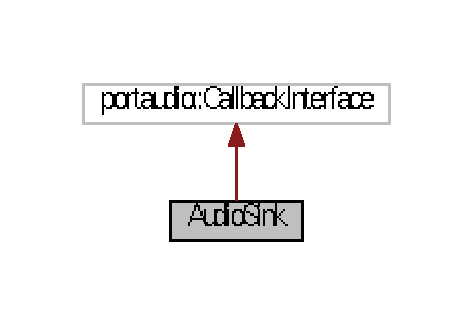
\includegraphics[width=227pt]{classAudioSink__inherit__graph}
\end{center}
\end{figure}


Collaboration diagram for Audio\+Sink\+:
\nopagebreak
\begin{figure}[H]
\begin{center}
\leavevmode
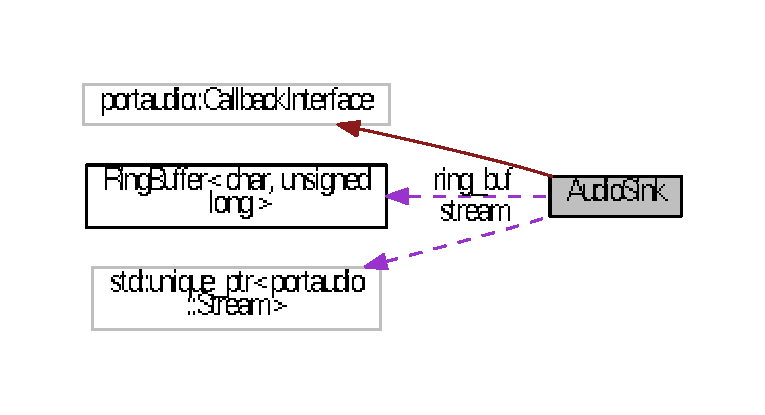
\includegraphics[width=350pt]{classAudioSink__coll__graph}
\end{center}
\end{figure}
\subsection*{Public Types}
\begin{DoxyCompactItemize}
\item 
using \hyperlink{classAudioSink_ae5b8370aa17c24c6fc8f8e0c5778168c}{Stream\+Configurator} = std\+::function$<$ portaudio\+::\+Stream $\ast$(portaudio\+::\+Callback\+Interface \&)$>$
\begin{DoxyCompactList}\small\item\em A function that configures and returns a stream, given this \hyperlink{classAudioSink}{Audio\+Sink}. \end{DoxyCompactList}\item 
\hypertarget{classAudioSink_a73002cc57611ac384c4e9d419e706e50}{using \hyperlink{classAudioSink_a73002cc57611ac384c4e9d419e706e50}{Play\+Callback\+Step\+Result} = std\+::pair$<$ Pa\+Stream\+Callback\+Result, unsigned long $>$}\label{classAudioSink_a73002cc57611ac384c4e9d419e706e50}

\begin{DoxyCompactList}\small\item\em Type of results emitted during the play callback step. \end{DoxyCompactList}\item 
\hypertarget{classAudioSink_ad2d7d33b3e937d057a4d72afad812737}{using \hyperlink{classAudioSink_ad2d7d33b3e937d057a4d72afad812737}{Sample\+Position} = std\+::uint64\+\_\+t}\label{classAudioSink_ad2d7d33b3e937d057a4d72afad812737}

\begin{DoxyCompactList}\small\item\em Type of positions measured in samples. \end{DoxyCompactList}\item 
\hypertarget{classAudioSink_a60c1743d66e02b77f04791e72fa4cd0b}{using \hyperlink{classAudioSink_a60c1743d66e02b77f04791e72fa4cd0b}{Transfer\+Iterator} = Audio\+Source\+::\+Decode\+Vector\+::iterator}\label{classAudioSink_a60c1743d66e02b77f04791e72fa4cd0b}

\begin{DoxyCompactList}\small\item\em Type of iterators used in the \hyperlink{classAudioSink_a455e211f4f16eaa21e7b75412cc8a8ae}{Transfer()} method. \end{DoxyCompactList}\end{DoxyCompactItemize}
\subsection*{Public Member Functions}
\begin{DoxyCompactItemize}
\item 
\hyperlink{classAudioSink_ab4adf46e3e93d35e2b5fb1ab0e75793b}{Audio\+Sink} (const \hyperlink{classAudioSink_ae5b8370aa17c24c6fc8f8e0c5778168c}{Stream\+Configurator} c, \hyperlink{classAudioSource_a1c8138ec9ffb9fd1394d0ad0782d60fa}{Audio\+Source\+::\+Sample\+Byte\+Count} \hyperlink{classAudioSink_a5eab0f7111187c0416feb542010e4a2e}{bytes\+\_\+per\+\_\+sample})
\begin{DoxyCompactList}\small\item\em Constructs an \hyperlink{classAudioSink}{Audio\+Sink}. \end{DoxyCompactList}\item 
void \hyperlink{classAudioSink_a18196e0dec3b4d58e17c454379ed0728}{Start} ()
\begin{DoxyCompactList}\small\item\em Starts the audio stream. \end{DoxyCompactList}\item 
void \hyperlink{classAudioSink_af1937ad09b555f0b88d285e8fd7cf433}{Stop} ()
\begin{DoxyCompactList}\small\item\em Stops the audio stream. \end{DoxyCompactList}\item 
bool \hyperlink{classAudioSink_adfa8006db0d1cbe161f15232cb32a324}{Is\+Stopped} ()
\begin{DoxyCompactList}\small\item\em Checks to see if audio playback has stopped. \end{DoxyCompactList}\item 
\hyperlink{classAudioSink_ad2d7d33b3e937d057a4d72afad812737}{Sample\+Position} \hyperlink{classAudioSink_aed168a8ce8ba39105431ab54ab08a007}{Position} ()
\begin{DoxyCompactList}\small\item\em Gets the current played position in the song, in samples. \end{DoxyCompactList}\item 
void \hyperlink{classAudioSink_a5ca539e3440d168eec0892114a947529}{Set\+Position} (\hyperlink{classAudioSink_ad2d7d33b3e937d057a4d72afad812737}{Sample\+Position} samples)
\begin{DoxyCompactList}\small\item\em Sets the current played position, given a position in samples. \end{DoxyCompactList}\item 
bool \hyperlink{classAudioSink_a9b3dbe861acd4bb7ac1903730a0a01f3}{Input\+Ready} ()
\begin{DoxyCompactList}\small\item\em Gets whether this \hyperlink{classAudioSink}{Audio\+Sink} is expecting input. \end{DoxyCompactList}\item 
void \hyperlink{classAudioSink_aaa92237f7ab548c1a898981f4dcd631c}{Set\+Input\+Ready} (bool ready)
\begin{DoxyCompactList}\small\item\em Set whether this \hyperlink{classAudioSink}{Audio\+Sink} can expect input. \end{DoxyCompactList}\item 
void \hyperlink{classAudioSink_a455e211f4f16eaa21e7b75412cc8a8ae}{Transfer} (\hyperlink{classAudioSink_a60c1743d66e02b77f04791e72fa4cd0b}{Transfer\+Iterator} \&start, const \hyperlink{classAudioSink_a60c1743d66e02b77f04791e72fa4cd0b}{Transfer\+Iterator} \&end)
\begin{DoxyCompactList}\small\item\em Transfers a range of sample bytes into the \hyperlink{classAudioSink}{Audio\+Sink}. \end{DoxyCompactList}\end{DoxyCompactItemize}
\subsection*{Private Member Functions}
\begin{DoxyCompactItemize}
\item 
int \hyperlink{classAudioSink_ad3534ea4210aa83b42706c0361fd3e8d}{pa\+Callback\+Fun} (const void $\ast$input\+Buffer, void $\ast$output\+Buffer, unsigned long num\+Frames, const Pa\+Stream\+Callback\+Time\+Info $\ast$time\+Info, Pa\+Stream\+Callback\+Flags status\+Flags) override
\begin{DoxyCompactList}\small\item\em The callback proper. \end{DoxyCompactList}\item 
\hyperlink{classAudioSink_a73002cc57611ac384c4e9d419e706e50}{Play\+Callback\+Step\+Result} \hyperlink{classAudioSink_a450ad1c0c64ddcc9b9a40d325983cbd9}{Play\+Callback\+Step} (char $\ast$out, unsigned long frames\+\_\+per\+\_\+buf, \hyperlink{classAudioSink_a73002cc57611ac384c4e9d419e706e50}{Play\+Callback\+Step\+Result} in)
\begin{DoxyCompactList}\small\item\em Performs one step in the callback. \end{DoxyCompactList}\item 
\hyperlink{classAudioSink_a73002cc57611ac384c4e9d419e706e50}{Play\+Callback\+Step\+Result} \hyperlink{classAudioSink_a2194fd0629b52c550c9eb326f8ae10cc}{Play\+Callback\+Success} (char $\ast$out, unsigned long avail, unsigned long frames\+\_\+per\+\_\+buf, \hyperlink{classAudioSink_a73002cc57611ac384c4e9d419e706e50}{Play\+Callback\+Step\+Result} in)
\begin{DoxyCompactList}\small\item\em Performs a successful play callback step. \end{DoxyCompactList}\item 
\hyperlink{classAudioSink_a73002cc57611ac384c4e9d419e706e50}{Play\+Callback\+Step\+Result} \hyperlink{classAudioSink_a6e1b9254b242231ba8168e5e27d602ff}{Play\+Callback\+Failure} (char $\ast$out, unsigned long avail, unsigned long frames\+\_\+per\+\_\+buf, \hyperlink{classAudioSink_a73002cc57611ac384c4e9d419e706e50}{Play\+Callback\+Step\+Result} in)
\begin{DoxyCompactList}\small\item\em Performs error cleanup for a failed play callback step. \end{DoxyCompactList}\item 
unsigned long \hyperlink{classAudioSink_a00ed918435d6f65b9533869453d5ae56}{Read\+Samples\+To\+Output} (char $\ast$\&output, unsigned long output\+\_\+capacity, unsigned long buffered\+\_\+count)
\begin{DoxyCompactList}\small\item\em Reads from the ringbuffer to output, updating the used samples count. \end{DoxyCompactList}\end{DoxyCompactItemize}
\subsection*{Private Attributes}
\begin{DoxyCompactItemize}
\item 
\hypertarget{classAudioSink_a5eab0f7111187c0416feb542010e4a2e}{\hyperlink{classAudioSource_a1c8138ec9ffb9fd1394d0ad0782d60fa}{Audio\+Source\+::\+Sample\+Byte\+Count} \hyperlink{classAudioSink_a5eab0f7111187c0416feb542010e4a2e}{bytes\+\_\+per\+\_\+sample}}\label{classAudioSink_a5eab0f7111187c0416feb542010e4a2e}

\begin{DoxyCompactList}\small\item\em Number of bytes in one sample. \end{DoxyCompactList}\item 
\hypertarget{classAudioSink_a87184f85d6cfcc7310043b877caeaee2}{\hyperlink{classRingBuffer}{Ring\+Buffer}$<$ char, unsigned long $>$ \hyperlink{classAudioSink_a87184f85d6cfcc7310043b877caeaee2}{ring\+\_\+buf}}\label{classAudioSink_a87184f85d6cfcc7310043b877caeaee2}

\begin{DoxyCompactList}\small\item\em The ring buffer used to transfer samples to the playing callback. \end{DoxyCompactList}\item 
\hypertarget{classAudioSink_aac90e7d95e98ac08b7c661a301eff1b2}{std\+::unique\+\_\+ptr\\*
$<$ portaudio\+::\+Stream $>$ \hyperlink{classAudioSink_aac90e7d95e98ac08b7c661a301eff1b2}{stream}}\label{classAudioSink_aac90e7d95e98ac08b7c661a301eff1b2}

\begin{DoxyCompactList}\small\item\em The Port\+Audio stream to which this \hyperlink{classAudioSink}{Audio\+Sink} outputs. \end{DoxyCompactList}\item 
\hypertarget{classAudioSink_ac3403a492b8aba8d483961d1ec09fa26}{std\+::uint64\+\_\+t \hyperlink{classAudioSink_ac3403a492b8aba8d483961d1ec09fa26}{position\+\_\+sample\+\_\+count}}\label{classAudioSink_ac3403a492b8aba8d483961d1ec09fa26}

\begin{DoxyCompactList}\small\item\em The current position, in samples. \end{DoxyCompactList}\item 
bool \hyperlink{classAudioSink_a00cbaaf2b4fcf5d9acb614b909234196}{just\+\_\+started}
\begin{DoxyCompactList}\small\item\em Whether the current run of the audio playback stream has not yet successfully read its first set of samples from the buffer. \end{DoxyCompactList}\item 
\hypertarget{classAudioSink_ad644a3477077e87f76cd24c9cb268f30}{bool \hyperlink{classAudioSink_ad644a3477077e87f76cd24c9cb268f30}{input\+\_\+ready}}\label{classAudioSink_ad644a3477077e87f76cd24c9cb268f30}

\begin{DoxyCompactList}\small\item\em Whether there is input ready for this sink. \end{DoxyCompactList}\end{DoxyCompactItemize}
\subsection*{Static Private Attributes}
\begin{DoxyCompactItemize}
\item 
static const size\+\_\+t \hyperlink{classAudioSink_a152e5a388d4570211509a2a19a38c321}{R\+I\+N\+G\+B\+U\+F\+\_\+\+P\+O\+W\+E\+R} = 16
\begin{DoxyCompactList}\small\item\em n, where 2$^\wedge$n is the capacity of the \hyperlink{classAudio}{Audio} ring buffer. \end{DoxyCompactList}\end{DoxyCompactItemize}


\subsection{Detailed Description}
An output stream for an \hyperlink{classAudio}{Audio} file. 

An \hyperlink{classAudioSink}{Audio\+Sink} consists of a Port\+Audio output stream and a buffer that stores decoded samples from the \hyperlink{classAudio}{Audio} object. While active, the \hyperlink{classAudioSink}{Audio\+Sink} periodically transfers samples from its buffer to Port\+Audio in a separate thread. 

Definition at line \hyperlink{audio__sink_8hpp_source_l00038}{38} of file \hyperlink{audio__sink_8hpp_source}{audio\+\_\+sink.\+hpp}.



\subsection{Member Typedef Documentation}
\hypertarget{classAudioSink_ae5b8370aa17c24c6fc8f8e0c5778168c}{\index{Audio\+Sink@{Audio\+Sink}!Stream\+Configurator@{Stream\+Configurator}}
\index{Stream\+Configurator@{Stream\+Configurator}!Audio\+Sink@{Audio\+Sink}}
\subsubsection[{Stream\+Configurator}]{\setlength{\rightskip}{0pt plus 5cm}using {\bf Audio\+Sink\+::\+Stream\+Configurator} =  std\+::function$<$ portaudio\+::\+Stream $\ast$(portaudio\+::\+Callback\+Interface \&)$>$}}\label{classAudioSink_ae5b8370aa17c24c6fc8f8e0c5778168c}


A function that configures and returns a stream, given this \hyperlink{classAudioSink}{Audio\+Sink}. 



Definition at line \hyperlink{audio__sink_8hpp_source_l00043}{43} of file \hyperlink{audio__sink_8hpp_source}{audio\+\_\+sink.\+hpp}.



\subsection{Constructor \& Destructor Documentation}
\hypertarget{classAudioSink_ab4adf46e3e93d35e2b5fb1ab0e75793b}{\index{Audio\+Sink@{Audio\+Sink}!Audio\+Sink@{Audio\+Sink}}
\index{Audio\+Sink@{Audio\+Sink}!Audio\+Sink@{Audio\+Sink}}
\subsubsection[{Audio\+Sink}]{\setlength{\rightskip}{0pt plus 5cm}Audio\+Sink\+::\+Audio\+Sink (
\begin{DoxyParamCaption}
\item[{const {\bf Stream\+Configurator}}]{c, }
\item[{{\bf Audio\+Source\+::\+Sample\+Byte\+Count}}]{bytes\+\_\+per\+\_\+sample}
\end{DoxyParamCaption}
)}}\label{classAudioSink_ab4adf46e3e93d35e2b5fb1ab0e75793b}


Constructs an \hyperlink{classAudioSink}{Audio\+Sink}. 


\begin{DoxyParams}{Parameters}
{\em c} & A function that can configure Port\+Audio streams. \\
\hline
{\em bytes\+\_\+per\+\_\+sample} & The number of bytes each audio sample occupies. \\
\hline
\end{DoxyParams}


Definition at line \hyperlink{audio__sink_8cpp_source_l00026}{26} of file \hyperlink{audio__sink_8cpp_source}{audio\+\_\+sink.\+cpp}.



References \hyperlink{audio__sink_8hpp_source_l00146}{stream}.


\begin{DoxyCode}
00028     : \hyperlink{classAudioSink_a5eab0f7111187c0416feb542010e4a2e}{bytes\_per\_sample}(\hyperlink{classAudioSink_a5eab0f7111187c0416feb542010e4a2e}{bytes\_per\_sample}),
00029       \hyperlink{classAudioSink_a87184f85d6cfcc7310043b877caeaee2}{ring\_buf}(\hyperlink{classAudioSink_a152e5a388d4570211509a2a19a38c321}{RINGBUF\_POWER}, \hyperlink{classAudioSink_a5eab0f7111187c0416feb542010e4a2e}{bytes\_per\_sample}),
00030       \hyperlink{classAudioSink_ac3403a492b8aba8d483961d1ec09fa26}{position\_sample\_count}(0),
00031       \hyperlink{classAudioSink_a00cbaaf2b4fcf5d9acb614b909234196}{just\_started}(\textcolor{keyword}{false}),
00032       \hyperlink{classAudioSink_ad644a3477077e87f76cd24c9cb268f30}{input\_ready}(\textcolor{keyword}{false})
00033 \{
00034     this->\hyperlink{classAudioSink_aac90e7d95e98ac08b7c661a301eff1b2}{stream} = decltype(this->\hyperlink{classAudioSink_aac90e7d95e98ac08b7c661a301eff1b2}{stream})(c(*\textcolor{keyword}{this}));
00035 \}
\end{DoxyCode}


\subsection{Member Function Documentation}
\hypertarget{classAudioSink_a9b3dbe861acd4bb7ac1903730a0a01f3}{\index{Audio\+Sink@{Audio\+Sink}!Input\+Ready@{Input\+Ready}}
\index{Input\+Ready@{Input\+Ready}!Audio\+Sink@{Audio\+Sink}}
\subsubsection[{Input\+Ready}]{\setlength{\rightskip}{0pt plus 5cm}bool Audio\+Sink\+::\+Input\+Ready (
\begin{DoxyParamCaption}
{}
\end{DoxyParamCaption}
)}}\label{classAudioSink_a9b3dbe861acd4bb7ac1903730a0a01f3}


Gets whether this \hyperlink{classAudioSink}{Audio\+Sink} is expecting input. 

\begin{DoxyReturn}{Returns}
Whether the input-\/ready flag has been set. 
\end{DoxyReturn}
\begin{DoxySeeAlso}{See also}
\hyperlink{classAudioSink_aaa92237f7ab548c1a898981f4dcd631c}{Set\+Input\+Ready} 
\end{DoxySeeAlso}


Definition at line \hyperlink{audio__sink_8cpp_source_l00055}{55} of file \hyperlink{audio__sink_8cpp_source}{audio\+\_\+sink.\+cpp}.



References \hyperlink{audio__sink_8hpp_source_l00156}{input\+\_\+ready}.



Referenced by \hyperlink{audio__sink_8cpp_source_l00156}{Play\+Callback\+Failure()}.


\begin{DoxyCode}
00056 \{
00057     \textcolor{keywordflow}{return} this->\hyperlink{classAudioSink_ad644a3477077e87f76cd24c9cb268f30}{input\_ready};
00058 \}
\end{DoxyCode}
\hypertarget{classAudioSink_adfa8006db0d1cbe161f15232cb32a324}{\index{Audio\+Sink@{Audio\+Sink}!Is\+Stopped@{Is\+Stopped}}
\index{Is\+Stopped@{Is\+Stopped}!Audio\+Sink@{Audio\+Sink}}
\subsubsection[{Is\+Stopped}]{\setlength{\rightskip}{0pt plus 5cm}bool Audio\+Sink\+::\+Is\+Stopped (
\begin{DoxyParamCaption}
{}
\end{DoxyParamCaption}
)}}\label{classAudioSink_adfa8006db0d1cbe161f15232cb32a324}


Checks to see if audio playback has stopped. 

\begin{DoxyReturn}{Returns}
True if the audio stream is inactive; false otherwise. 
\end{DoxyReturn}
\begin{DoxySeeAlso}{See also}
\hyperlink{classAudioSink_a18196e0dec3b4d58e17c454379ed0728}{Start} 

\hyperlink{classAudioSink_af1937ad09b555f0b88d285e8fd7cf433}{Stop} 
\end{DoxySeeAlso}


Definition at line \hyperlink{audio__sink_8cpp_source_l00050}{50} of file \hyperlink{audio__sink_8cpp_source}{audio\+\_\+sink.\+cpp}.



References \hyperlink{audio__sink_8hpp_source_l00146}{stream}.


\begin{DoxyCode}
00051 \{
00052     \textcolor{keywordflow}{return} !this->\hyperlink{classAudioSink_aac90e7d95e98ac08b7c661a301eff1b2}{stream}->isActive();
00053 \}
\end{DoxyCode}
\hypertarget{classAudioSink_ad3534ea4210aa83b42706c0361fd3e8d}{\index{Audio\+Sink@{Audio\+Sink}!pa\+Callback\+Fun@{pa\+Callback\+Fun}}
\index{pa\+Callback\+Fun@{pa\+Callback\+Fun}!Audio\+Sink@{Audio\+Sink}}
\subsubsection[{pa\+Callback\+Fun}]{\setlength{\rightskip}{0pt plus 5cm}int Audio\+Sink\+::pa\+Callback\+Fun (
\begin{DoxyParamCaption}
\item[{const void $\ast$}]{input\+Buffer, }
\item[{void $\ast$}]{output\+Buffer, }
\item[{unsigned long}]{num\+Frames, }
\item[{const Pa\+Stream\+Callback\+Time\+Info $\ast$}]{time\+Info, }
\item[{Pa\+Stream\+Callback\+Flags}]{status\+Flags}
\end{DoxyParamCaption}
)\hspace{0.3cm}{\ttfamily [override]}, {\ttfamily [private]}}}\label{classAudioSink_ad3534ea4210aa83b42706c0361fd3e8d}


The callback proper. 

This is executed in a separate thread by Port\+Audio once a stream is playing with the callback registered to it. 
\begin{DoxyParams}{Parameters}
{\em input\+Buffer} & The buffer containing input data; ignored. \\
\hline
{\em output\+Buffer} & The output buffer to which our samples should be written. \\
\hline
{\em num\+Frames} & The number of samples Port\+Audio wants to read from {\itshape output\+Buffer}. \\
\hline
{\em time\+Info} & The time information from Port\+Audio; ignored. \\
\hline
{\em status\+Flags} & The Port\+Audio status flags; ignored. \\
\hline
\end{DoxyParams}
\begin{DoxyReturn}{Returns}
The number of samples written to the output buffer. 
\end{DoxyReturn}


Definition at line \hyperlink{audio__sink_8cpp_source_l00110}{110} of file \hyperlink{audio__sink_8cpp_source}{audio\+\_\+sink.\+cpp}.



References \hyperlink{audio__sink_8cpp_source_l00126}{Play\+Callback\+Step()}.


\begin{DoxyCode}
00114 \{
00115     \textcolor{keywordtype}{char} *cout = \textcolor{keyword}{static\_cast<}\textcolor{keywordtype}{char} *\textcolor{keyword}{>}(out);
00116 
00117     std::pair<PaStreamCallbackResult, unsigned long> result =
00118                     std::make\_pair(paContinue, 0);
00119 
00120     \textcolor{keywordflow}{while} (result.first == paContinue && result.second < frames\_per\_buf) \{
00121         result = \hyperlink{classAudioSink_a450ad1c0c64ddcc9b9a40d325983cbd9}{PlayCallbackStep}(cout, frames\_per\_buf, result);
00122     \}
00123     \textcolor{keywordflow}{return} \textcolor{keyword}{static\_cast<}\textcolor{keywordtype}{int}\textcolor{keyword}{>}(result.first);
00124 \}
\end{DoxyCode}
\hypertarget{classAudioSink_a6e1b9254b242231ba8168e5e27d602ff}{\index{Audio\+Sink@{Audio\+Sink}!Play\+Callback\+Failure@{Play\+Callback\+Failure}}
\index{Play\+Callback\+Failure@{Play\+Callback\+Failure}!Audio\+Sink@{Audio\+Sink}}
\subsubsection[{Play\+Callback\+Failure}]{\setlength{\rightskip}{0pt plus 5cm}{\bf Play\+Callback\+Step\+Result} Audio\+Sink\+::\+Play\+Callback\+Failure (
\begin{DoxyParamCaption}
\item[{char $\ast$}]{out, }
\item[{unsigned long}]{avail, }
\item[{unsigned long}]{frames\+\_\+per\+\_\+buf, }
\item[{{\bf Play\+Callback\+Step\+Result}}]{in}
\end{DoxyParamCaption}
)\hspace{0.3cm}{\ttfamily [private]}}}\label{classAudioSink_a6e1b9254b242231ba8168e5e27d602ff}


Performs error cleanup for a failed play callback step. 

This ensures that the output buffer is filled with silence and the correct error code is returned. 
\begin{DoxyParams}{Parameters}
{\em out} & The output buffer to which our samples should be written. \\
\hline
{\em avail} & The number of samples available in the ring buffer. \\
\hline
{\em frames\+\_\+per\+\_\+buf} & The number of samples Port\+Audio wants to read {\itshape out}. \\
\hline
{\em in} & The result from the previous Play\+Callback\+Step. \\
\hline
\end{DoxyParams}
\begin{DoxyReturn}{Returns}
A Play\+Callback\+Step\+Result containing the status code and number of samples written as of the end of this step. 
\end{DoxyReturn}


Definition at line \hyperlink{audio__sink_8cpp_source_l00156}{156} of file \hyperlink{audio__sink_8cpp_source}{audio\+\_\+sink.\+cpp}.



References \hyperlink{audio__sink_8hpp_source_l00140}{bytes\+\_\+per\+\_\+sample}, and \hyperlink{audio__sink_8cpp_source_l00055}{Input\+Ready()}.



Referenced by \hyperlink{audio__sink_8cpp_source_l00126}{Play\+Callback\+Step()}.


\begin{DoxyCode}
00159 \{
00160     decltype(in) result;
00161 
00162     if (\hyperlink{classAudioSink_a9b3dbe861acd4bb7ac1903730a0a01f3}{InputReady}()) \{
00163         \textcolor{comment}{// There's been some sort of genuine issue.}
00164         \textcolor{comment}{// Make up some silence to plug the gap.}
00165         \hyperlink{classDebug}{Debug}() << \textcolor{stringliteral}{"Buffer underflow"} << std::endl;
00166         memset(out, 0, this->\hyperlink{classAudioSink_a5eab0f7111187c0416feb542010e4a2e}{bytes\_per\_sample} * frames\_per\_buf);
00167         result = std::make\_pair(paContinue, frames\_per\_buf);
00168     \} \textcolor{keywordflow}{else} \{
00169         \textcolor{comment}{// End of input is ok, it means the stream can finish.}
00170         result = std::make\_pair(paComplete, in.second);
00171     \}
00172 
00173     \textcolor{keywordflow}{return} result;
00174 \}
\end{DoxyCode}
\hypertarget{classAudioSink_a450ad1c0c64ddcc9b9a40d325983cbd9}{\index{Audio\+Sink@{Audio\+Sink}!Play\+Callback\+Step@{Play\+Callback\+Step}}
\index{Play\+Callback\+Step@{Play\+Callback\+Step}!Audio\+Sink@{Audio\+Sink}}
\subsubsection[{Play\+Callback\+Step}]{\setlength{\rightskip}{0pt plus 5cm}{\bf Play\+Callback\+Step\+Result} Audio\+Sink\+::\+Play\+Callback\+Step (
\begin{DoxyParamCaption}
\item[{char $\ast$}]{out, }
\item[{unsigned long}]{frames\+\_\+per\+\_\+buf, }
\item[{{\bf Play\+Callback\+Step\+Result}}]{in}
\end{DoxyParamCaption}
)\hspace{0.3cm}{\ttfamily [private]}}}\label{classAudioSink_a450ad1c0c64ddcc9b9a40d325983cbd9}


Performs one step in the callback. 


\begin{DoxyParams}{Parameters}
{\em out} & The output buffer to which our samples should be written. \\
\hline
{\em frames\+\_\+per\+\_\+buf} & The number of samples Port\+Audio wants to read {\itshape out}. \\
\hline
{\em in} & The result from the previous Play\+Callback\+Step. \\
\hline
\end{DoxyParams}
\begin{DoxyReturn}{Returns}
A Play\+Callback\+Step\+Result containing the status code and number of samples written as of the end of this step. 
\end{DoxyReturn}


Definition at line \hyperlink{audio__sink_8cpp_source_l00126}{126} of file \hyperlink{audio__sink_8cpp_source}{audio\+\_\+sink.\+cpp}.



References \hyperlink{audio__sink_8hpp_source_l00153}{just\+\_\+started}, \hyperlink{audio__sink_8cpp_source_l00156}{Play\+Callback\+Failure()}, \hyperlink{audio__sink_8cpp_source_l00144}{Play\+Callback\+Success()}, \hyperlink{ringbuffer_8hpp_source_l00093}{Ring\+Buffer$<$ Rep\+T, Sample\+Count\+T $>$\+::\+Read\+Capacity()}, and \hyperlink{audio__sink_8hpp_source_l00143}{ring\+\_\+buf}.



Referenced by \hyperlink{audio__sink_8cpp_source_l00110}{pa\+Callback\+Fun()}.


\begin{DoxyCode}
00129 \{
00130     \textcolor{keywordtype}{unsigned} \textcolor{keywordtype}{long} avail = this->\hyperlink{classAudioSink_a87184f85d6cfcc7310043b877caeaee2}{ring\_buf}.\hyperlink{classRingBuffer_a7086cc66306105db205842af7a88c2d8}{ReadCapacity}();
00131     \textcolor{keywordtype}{bool} empty = avail == 0;
00132 
00133     \textcolor{comment}{/* If we've just started this stream, we don't want to hand PortAudio}
00134 \textcolor{comment}{       an incomplete frame—we'd rather wait until we have enough in the}
00135 \textcolor{comment}{       ring buffer before starting to play out. */}
00136     \textcolor{keywordtype}{bool} wait = this->\hyperlink{classAudioSink_a00cbaaf2b4fcf5d9acb614b909234196}{just\_started} && (avail < frames\_per\_buf);
00137 
00138     \textcolor{keywordtype}{bool} failed = wait || empty;
00139     \textcolor{keyword}{auto} fn = failed ? &\hyperlink{classAudioSink_a6e1b9254b242231ba8168e5e27d602ff}{AudioSink::PlayCallbackFailure}
00140                      : &\hyperlink{classAudioSink_a2194fd0629b52c550c9eb326f8ae10cc}{AudioSink::PlayCallbackSuccess};
00141     \textcolor{keywordflow}{return} (this->*fn)(out, avail, frames\_per\_buf, in);
00142 \}
\end{DoxyCode}
\hypertarget{classAudioSink_a2194fd0629b52c550c9eb326f8ae10cc}{\index{Audio\+Sink@{Audio\+Sink}!Play\+Callback\+Success@{Play\+Callback\+Success}}
\index{Play\+Callback\+Success@{Play\+Callback\+Success}!Audio\+Sink@{Audio\+Sink}}
\subsubsection[{Play\+Callback\+Success}]{\setlength{\rightskip}{0pt plus 5cm}{\bf Play\+Callback\+Step\+Result} Audio\+Sink\+::\+Play\+Callback\+Success (
\begin{DoxyParamCaption}
\item[{char $\ast$}]{out, }
\item[{unsigned long}]{avail, }
\item[{unsigned long}]{frames\+\_\+per\+\_\+buf, }
\item[{{\bf Play\+Callback\+Step\+Result}}]{in}
\end{DoxyParamCaption}
)\hspace{0.3cm}{\ttfamily [private]}}}\label{classAudioSink_a2194fd0629b52c550c9eb326f8ae10cc}


Performs a successful play callback step. 

This ensures that the appropriate number of samples are read into Port\+Audio's buffer. 
\begin{DoxyParams}{Parameters}
{\em out} & The output buffer to which our samples should be written. \\
\hline
{\em avail} & The number of samples available in the ring buffer. \\
\hline
{\em frames\+\_\+per\+\_\+buf} & The number of samples Port\+Audio wants to read {\itshape out}. \\
\hline
{\em in} & The result from the previous Play\+Callback\+Step. \\
\hline
\end{DoxyParams}
\begin{DoxyReturn}{Returns}
A Play\+Callback\+Step\+Result containing the status code and number of samples written as of the end of this step. 
\end{DoxyReturn}


Definition at line \hyperlink{audio__sink_8cpp_source_l00144}{144} of file \hyperlink{audio__sink_8cpp_source}{audio\+\_\+sink.\+cpp}.



References \hyperlink{audio__sink_8hpp_source_l00153}{just\+\_\+started}, and \hyperlink{audio__sink_8cpp_source_l00176}{Read\+Samples\+To\+Output()}.



Referenced by \hyperlink{audio__sink_8cpp_source_l00126}{Play\+Callback\+Step()}.


\begin{DoxyCode}
00147 \{
00148     this->\hyperlink{classAudioSink_a00cbaaf2b4fcf5d9acb614b909234196}{just\_started} = \textcolor{keyword}{false};
00149 
00150     \textcolor{keyword}{auto} samples\_pa\_wants = frames\_per\_buf - in.second;
00151     \textcolor{keyword}{auto} samples\_read = \hyperlink{classAudioSink_a00ed918435d6f65b9533869453d5ae56}{ReadSamplesToOutput}(out, avail, samples\_pa\_wants);
00152 
00153     \textcolor{keywordflow}{return} std::make\_pair(paContinue, in.second + samples\_read);
00154 \}
\end{DoxyCode}
\hypertarget{classAudioSink_aed168a8ce8ba39105431ab54ab08a007}{\index{Audio\+Sink@{Audio\+Sink}!Position@{Position}}
\index{Position@{Position}!Audio\+Sink@{Audio\+Sink}}
\subsubsection[{Position}]{\setlength{\rightskip}{0pt plus 5cm}{\bf Audio\+Sink\+::\+Sample\+Position} Audio\+Sink\+::\+Position (
\begin{DoxyParamCaption}
{}
\end{DoxyParamCaption}
)}}\label{classAudioSink_aed168a8ce8ba39105431ab54ab08a007}


Gets the current played position in the song, in samples. 

As this may be executing whilst the playing callback is running, do not expect it to be highly accurate. \begin{DoxyReturn}{Returns}
The current position, as a count of elapsed samples. 
\end{DoxyReturn}
\begin{DoxySeeAlso}{See also}
\hyperlink{classAudioSink_ad2d7d33b3e937d057a4d72afad812737}{Sample\+Position} 
\end{DoxySeeAlso}


Definition at line \hyperlink{audio__sink_8cpp_source_l00065}{65} of file \hyperlink{audio__sink_8cpp_source}{audio\+\_\+sink.\+cpp}.



References \hyperlink{audio__sink_8hpp_source_l00149}{position\+\_\+sample\+\_\+count}.


\begin{DoxyCode}
00066 \{
00067     \textcolor{keywordflow}{return} this->\hyperlink{classAudioSink_ac3403a492b8aba8d483961d1ec09fa26}{position\_sample\_count};
00068 \}
\end{DoxyCode}
\hypertarget{classAudioSink_a00ed918435d6f65b9533869453d5ae56}{\index{Audio\+Sink@{Audio\+Sink}!Read\+Samples\+To\+Output@{Read\+Samples\+To\+Output}}
\index{Read\+Samples\+To\+Output@{Read\+Samples\+To\+Output}!Audio\+Sink@{Audio\+Sink}}
\subsubsection[{Read\+Samples\+To\+Output}]{\setlength{\rightskip}{0pt plus 5cm}unsigned long Audio\+Sink\+::\+Read\+Samples\+To\+Output (
\begin{DoxyParamCaption}
\item[{char $\ast$\&}]{output, }
\item[{unsigned long}]{output\+\_\+capacity, }
\item[{unsigned long}]{buffered\+\_\+count}
\end{DoxyParamCaption}
)\hspace{0.3cm}{\ttfamily [private]}}}\label{classAudioSink_a00ed918435d6f65b9533869453d5ae56}


Reads from the ringbuffer to output, updating the used samples count. 


\begin{DoxyParams}{Parameters}
{\em output} & A reference to the output buffer's current pointer. \\
\hline
{\em output\+\_\+capacity} & The capacity of the output buffer, in samples. \\
\hline
{\em buffered\+\_\+count} & The number of samples available in the ring buffer. \\
\hline
\end{DoxyParams}
\begin{DoxyReturn}{Returns}
The number of samples successfully written to the output buffer. 
\end{DoxyReturn}


Definition at line \hyperlink{audio__sink_8cpp_source_l00176}{176} of file \hyperlink{audio__sink_8cpp_source}{audio\+\_\+sink.\+cpp}.



References \hyperlink{audio__sink_8hpp_source_l00149}{position\+\_\+sample\+\_\+count}, \hyperlink{ringbuffer_8hpp_source_l00149}{Ring\+Buffer$<$ Rep\+T, Sample\+Count\+T $>$\+::\+Read()}, and \hyperlink{audio__sink_8hpp_source_l00143}{ring\+\_\+buf}.



Referenced by \hyperlink{audio__sink_8cpp_source_l00144}{Play\+Callback\+Success()}.


\begin{DoxyCode}
00179 \{
00180     \textcolor{comment}{// Transfer the maximum that we can offer to PortAudio without}
00181     \textcolor{comment}{// overshooting}
00182     \textcolor{comment}{// its sample request limit.}
00183     \textcolor{keywordtype}{long} transfer\_sample\_count = \textcolor{keyword}{static\_cast<}\textcolor{keywordtype}{long}\textcolor{keyword}{>}(
00184                     std::min(\{ output\_capacity, buffered\_count,
00185                            \textcolor{keyword}{static\_cast<}\textcolor{keywordtype}{unsigned} \textcolor{keywordtype}{long}\textcolor{keyword}{>}(LONG\_MAX) \}));
00186     output += this->\hyperlink{classAudioSink_a87184f85d6cfcc7310043b877caeaee2}{ring\_buf}.\hyperlink{classRingBuffer_af892330ee102bd50a493b8afa814a0f0}{Read}(output, transfer\_sample\_count);
00187 
00188     \textcolor{comment}{// Update the position count so it reflects the last position that was}
00189     \textcolor{comment}{// sent}
00190     \textcolor{comment}{// for playback (*not* the last position decoded).}
00191     this->\hyperlink{classAudioSink_ac3403a492b8aba8d483961d1ec09fa26}{position\_sample\_count} += transfer\_sample\_count;
00192     \textcolor{keywordflow}{return} transfer\_sample\_count;
00193 \}
\end{DoxyCode}
\hypertarget{classAudioSink_aaa92237f7ab548c1a898981f4dcd631c}{\index{Audio\+Sink@{Audio\+Sink}!Set\+Input\+Ready@{Set\+Input\+Ready}}
\index{Set\+Input\+Ready@{Set\+Input\+Ready}!Audio\+Sink@{Audio\+Sink}}
\subsubsection[{Set\+Input\+Ready}]{\setlength{\rightskip}{0pt plus 5cm}void Audio\+Sink\+::\+Set\+Input\+Ready (
\begin{DoxyParamCaption}
\item[{bool}]{ready}
\end{DoxyParamCaption}
)}}\label{classAudioSink_aaa92237f7ab548c1a898981f4dcd631c}


Set whether this \hyperlink{classAudioSink}{Audio\+Sink} can expect input. 


\begin{DoxyParams}{Parameters}
{\em ready} & True if there is input ready; false otherwise. \\
\hline
\end{DoxyParams}
\begin{DoxySeeAlso}{See also}
\hyperlink{classAudioSink_a9b3dbe861acd4bb7ac1903730a0a01f3}{Input\+Ready} 
\end{DoxySeeAlso}


Definition at line \hyperlink{audio__sink_8cpp_source_l00060}{60} of file \hyperlink{audio__sink_8cpp_source}{audio\+\_\+sink.\+cpp}.



References \hyperlink{audio__sink_8hpp_source_l00156}{input\+\_\+ready}.


\begin{DoxyCode}
00061 \{
00062     this->\hyperlink{classAudioSink_ad644a3477077e87f76cd24c9cb268f30}{input\_ready} = ready;
00063 \}
\end{DoxyCode}
\hypertarget{classAudioSink_a5ca539e3440d168eec0892114a947529}{\index{Audio\+Sink@{Audio\+Sink}!Set\+Position@{Set\+Position}}
\index{Set\+Position@{Set\+Position}!Audio\+Sink@{Audio\+Sink}}
\subsubsection[{Set\+Position}]{\setlength{\rightskip}{0pt plus 5cm}void Audio\+Sink\+::\+Set\+Position (
\begin{DoxyParamCaption}
\item[{{\bf Audio\+Sink\+::\+Sample\+Position}}]{samples}
\end{DoxyParamCaption}
)}}\label{classAudioSink_a5ca539e3440d168eec0892114a947529}


Sets the current played position, given a position in samples. 

This flushes out the \hyperlink{classAudioSink}{Audio\+Sink} ready to receive sample data from the new position. 
\begin{DoxyParams}{Parameters}
{\em samples} & The new position, as a count of elapsed samples. \\
\hline
\end{DoxyParams}
\begin{DoxySeeAlso}{See also}
\hyperlink{classAudioSink_aed168a8ce8ba39105431ab54ab08a007}{Position} 
\end{DoxySeeAlso}


Definition at line \hyperlink{audio__sink_8cpp_source_l00070}{70} of file \hyperlink{audio__sink_8cpp_source}{audio\+\_\+sink.\+cpp}.



References \hyperlink{ringbuffer_8hpp_source_l00160}{Ring\+Buffer$<$ Rep\+T, Sample\+Count\+T $>$\+::\+Flush()}, \hyperlink{audio__sink_8hpp_source_l00149}{position\+\_\+sample\+\_\+count}, and \hyperlink{audio__sink_8hpp_source_l00143}{ring\+\_\+buf}.


\begin{DoxyCode}
00071 \{
00072     this->\hyperlink{classAudioSink_ac3403a492b8aba8d483961d1ec09fa26}{position\_sample\_count} = samples;
00073     this->\hyperlink{classAudioSink_a87184f85d6cfcc7310043b877caeaee2}{ring\_buf}.\hyperlink{classRingBuffer_a1eb1acca6905e7678fbbdb70238cdc26}{Flush}();
00074 \}
\end{DoxyCode}
\hypertarget{classAudioSink_a18196e0dec3b4d58e17c454379ed0728}{\index{Audio\+Sink@{Audio\+Sink}!Start@{Start}}
\index{Start@{Start}!Audio\+Sink@{Audio\+Sink}}
\subsubsection[{Start}]{\setlength{\rightskip}{0pt plus 5cm}void Audio\+Sink\+::\+Start (
\begin{DoxyParamCaption}
{}
\end{DoxyParamCaption}
)}}\label{classAudioSink_a18196e0dec3b4d58e17c454379ed0728}


Starts the audio stream. 

\begin{DoxySeeAlso}{See also}
\hyperlink{classAudioSink_af1937ad09b555f0b88d285e8fd7cf433}{Stop} 

Is\+Halted 
\end{DoxySeeAlso}


Definition at line \hyperlink{audio__sink_8cpp_source_l00037}{37} of file \hyperlink{audio__sink_8cpp_source}{audio\+\_\+sink.\+cpp}.



References \hyperlink{audio__sink_8hpp_source_l00153}{just\+\_\+started}, and \hyperlink{audio__sink_8hpp_source_l00146}{stream}.


\begin{DoxyCode}
00038 \{
00039     this->\hyperlink{classAudioSink_a00cbaaf2b4fcf5d9acb614b909234196}{just\_started} = \textcolor{keyword}{true};
00040     this->\hyperlink{classAudioSink_aac90e7d95e98ac08b7c661a301eff1b2}{stream}->start();
00041 \}
\end{DoxyCode}
\hypertarget{classAudioSink_af1937ad09b555f0b88d285e8fd7cf433}{\index{Audio\+Sink@{Audio\+Sink}!Stop@{Stop}}
\index{Stop@{Stop}!Audio\+Sink@{Audio\+Sink}}
\subsubsection[{Stop}]{\setlength{\rightskip}{0pt plus 5cm}void Audio\+Sink\+::\+Stop (
\begin{DoxyParamCaption}
{}
\end{DoxyParamCaption}
)}}\label{classAudioSink_af1937ad09b555f0b88d285e8fd7cf433}


Stops the audio stream. 

\begin{DoxySeeAlso}{See also}
\hyperlink{classAudioSink_a18196e0dec3b4d58e17c454379ed0728}{Start} 

Is\+Halted 
\end{DoxySeeAlso}


Definition at line \hyperlink{audio__sink_8cpp_source_l00043}{43} of file \hyperlink{audio__sink_8cpp_source}{audio\+\_\+sink.\+cpp}.



References \hyperlink{audio__sink_8hpp_source_l00146}{stream}.


\begin{DoxyCode}
00044 \{
00045     \textcolor{keywordflow}{if} (!this->\hyperlink{classAudioSink_aac90e7d95e98ac08b7c661a301eff1b2}{stream}->isStopped()) \{
00046         this->\hyperlink{classAudioSink_aac90e7d95e98ac08b7c661a301eff1b2}{stream}->abort();
00047     \}
00048 \}
\end{DoxyCode}
\hypertarget{classAudioSink_a455e211f4f16eaa21e7b75412cc8a8ae}{\index{Audio\+Sink@{Audio\+Sink}!Transfer@{Transfer}}
\index{Transfer@{Transfer}!Audio\+Sink@{Audio\+Sink}}
\subsubsection[{Transfer}]{\setlength{\rightskip}{0pt plus 5cm}void Audio\+Sink\+::\+Transfer (
\begin{DoxyParamCaption}
\item[{{\bf Audio\+Sink\+::\+Transfer\+Iterator} \&}]{start, }
\item[{const {\bf Transfer\+Iterator} \&}]{end}
\end{DoxyParamCaption}
)}}\label{classAudioSink_a455e211f4f16eaa21e7b75412cc8a8ae}


Transfers a range of sample bytes into the \hyperlink{classAudioSink}{Audio\+Sink}. 

The range may be empty, but must be valid.


\begin{DoxyItemize}
\item Precondition\+: {\itshape start} $<$= {\itshape end}, {\itshape start} and {\itshape end} point to a valid contiguous block of sample bytes.
\item Postcondition\+: {\itshape start} $<$= {\itshape end}, {\itshape old(start)} $<$= {\itshape start}, {\itshape $\ast$start} and {\itshape end} point to a valid contiguous block of sample bytes.
\end{DoxyItemize}


\begin{DoxyParams}{Parameters}
{\em start} & An iterator denoting the start of the range. This iterator will be advanced by the number of bytes accepted. \\
\hline
{\em end} & An iterator denoting the end of the range. \\
\hline
\end{DoxyParams}


Definition at line \hyperlink{audio__sink_8cpp_source_l00076}{76} of file \hyperlink{audio__sink_8cpp_source}{audio\+\_\+sink.\+cpp}.



References \hyperlink{audio__sink_8hpp_source_l00140}{bytes\+\_\+per\+\_\+sample}, \hyperlink{audio__sink_8hpp_source_l00143}{ring\+\_\+buf}, \hyperlink{ringbuffer_8hpp_source_l00120}{Ring\+Buffer$<$ Rep\+T, Sample\+Count\+T $>$\+::\+Write()}, and \hyperlink{ringbuffer_8hpp_source_l00083}{Ring\+Buffer$<$ Rep\+T, Sample\+Count\+T $>$\+::\+Write\+Capacity()}.


\begin{DoxyCode}
00078 \{
00079     \textcolor{comment}{// No point transferring 0 bytes.}
00080     \textcolor{keywordflow}{if} (start == end) \{
00081         \textcolor{keywordflow}{return};
00082     \}
00083     assert(start < end);
00084 
00085     \textcolor{keywordtype}{unsigned} \textcolor{keywordtype}{long} bytes = std::distance(start, end);
00086     \textcolor{comment}{// There should be a whole number of samples being transferred.}
00087     assert(bytes % \hyperlink{classAudioSink_a5eab0f7111187c0416feb542010e4a2e}{bytes\_per\_sample} == 0);
00088     assert(0 < bytes);
00089 
00090     \textcolor{keyword}{auto} samples = bytes / this->\hyperlink{classAudioSink_a5eab0f7111187c0416feb542010e4a2e}{bytes\_per\_sample};
00091 
00092     \textcolor{comment}{// Only transfer as many samples as the ring buffer can take.}
00093     \textcolor{comment}{// Don't bother trying to write 0 samples!}
00094     \textcolor{keyword}{auto} count = std::min(samples, this->\hyperlink{classAudioSink_a87184f85d6cfcc7310043b877caeaee2}{ring\_buf}.\hyperlink{classRingBuffer_ab00617ab6e379ad146cb7b80079f4c4c}{WriteCapacity}());
00095     \textcolor{keywordflow}{if} (count == 0) \{
00096         \textcolor{keywordflow}{return};
00097     \}
00098     assert(0 < count);
00099 
00100     \textcolor{keyword}{auto} start\_ptr = \textcolor{keyword}{reinterpret\_cast<}\textcolor{keywordtype}{char} *\textcolor{keyword}{>}(&*start);
00101     \textcolor{keywordtype}{unsigned} \textcolor{keywordtype}{long} written\_count = this->\hyperlink{classAudioSink_a87184f85d6cfcc7310043b877caeaee2}{ring\_buf}.\hyperlink{classRingBuffer_aa7f863968cb641946b0cf341bda11e16}{Write}(start\_ptr, count);
00102     \textcolor{comment}{// Since we never write more than the ring buffer can take, the written}
00103     \textcolor{comment}{// count should equal the requested written count.}
00104     assert(written\_count == count);
00105 
00106     start += (written\_count * this->\hyperlink{classAudioSink_a5eab0f7111187c0416feb542010e4a2e}{bytes\_per\_sample});
00107     assert(start <= end);
00108 \}
\end{DoxyCode}


\subsection{Member Data Documentation}
\hypertarget{classAudioSink_a00cbaaf2b4fcf5d9acb614b909234196}{\index{Audio\+Sink@{Audio\+Sink}!just\+\_\+started@{just\+\_\+started}}
\index{just\+\_\+started@{just\+\_\+started}!Audio\+Sink@{Audio\+Sink}}
\subsubsection[{just\+\_\+started}]{\setlength{\rightskip}{0pt plus 5cm}bool Audio\+Sink\+::just\+\_\+started\hspace{0.3cm}{\ttfamily [private]}}}\label{classAudioSink_a00cbaaf2b4fcf5d9acb614b909234196}


Whether the current run of the audio playback stream has not yet successfully read its first set of samples from the buffer. 



Definition at line \hyperlink{audio__sink_8hpp_source_l00153}{153} of file \hyperlink{audio__sink_8hpp_source}{audio\+\_\+sink.\+hpp}.



Referenced by \hyperlink{audio__sink_8cpp_source_l00126}{Play\+Callback\+Step()}, \hyperlink{audio__sink_8cpp_source_l00144}{Play\+Callback\+Success()}, and \hyperlink{audio__sink_8cpp_source_l00037}{Start()}.

\hypertarget{classAudioSink_a152e5a388d4570211509a2a19a38c321}{\index{Audio\+Sink@{Audio\+Sink}!R\+I\+N\+G\+B\+U\+F\+\_\+\+P\+O\+W\+E\+R@{R\+I\+N\+G\+B\+U\+F\+\_\+\+P\+O\+W\+E\+R}}
\index{R\+I\+N\+G\+B\+U\+F\+\_\+\+P\+O\+W\+E\+R@{R\+I\+N\+G\+B\+U\+F\+\_\+\+P\+O\+W\+E\+R}!Audio\+Sink@{Audio\+Sink}}
\subsubsection[{R\+I\+N\+G\+B\+U\+F\+\_\+\+P\+O\+W\+E\+R}]{\setlength{\rightskip}{0pt plus 5cm}const size\+\_\+t Audio\+Sink\+::\+R\+I\+N\+G\+B\+U\+F\+\_\+\+P\+O\+W\+E\+R = 16\hspace{0.3cm}{\ttfamily [static]}, {\ttfamily [private]}}}\label{classAudioSink_a152e5a388d4570211509a2a19a38c321}


n, where 2$^\wedge$n is the capacity of the \hyperlink{classAudio}{Audio} ring buffer. 

\begin{DoxySeeAlso}{See also}
R\+I\+N\+G\+B\+U\+F\+\_\+\+S\+I\+Z\+E 
\end{DoxySeeAlso}


Definition at line \hyperlink{audio__sink_8hpp_source_l00137}{137} of file \hyperlink{audio__sink_8hpp_source}{audio\+\_\+sink.\+hpp}.



The documentation for this class was generated from the following files\+:\begin{DoxyCompactItemize}
\item 
src/audio/\hyperlink{audio__sink_8hpp}{audio\+\_\+sink.\+hpp}\item 
src/audio/\hyperlink{audio__sink_8cpp}{audio\+\_\+sink.\+cpp}\end{DoxyCompactItemize}

\hypertarget{classAudioSource}{\section{Audio\+Source Class Reference}
\label{classAudioSource}\index{Audio\+Source@{Audio\+Source}}
}


An object responsible for decoding an audio file.  




{\ttfamily \#include $<$audio\+\_\+source.\+hpp$>$}



Collaboration diagram for Audio\+Source\+:
\nopagebreak
\begin{figure}[H]
\begin{center}
\leavevmode
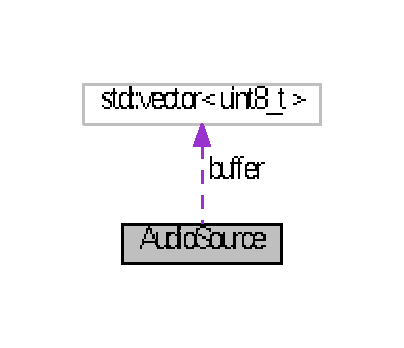
\includegraphics[width=194pt]{classAudioSource__coll__graph}
\end{center}
\end{figure}
\subsection*{Public Types}
\begin{DoxyCompactItemize}
\item 
enum \hyperlink{classAudioSource_a9a2f5de44325c84e69a7af1331aa159d}{Decode\+State} \+: std\+::uint8\+\_\+t \{ \hyperlink{classAudioSource_a9a2f5de44325c84e69a7af1331aa159da22a62bc6e9b3fff5866c4259f046bad8}{Decode\+State\+::\+W\+A\+I\+T\+I\+N\+G\+\_\+\+F\+O\+R\+\_\+\+F\+R\+A\+M\+E}, 
\hyperlink{classAudioSource_a9a2f5de44325c84e69a7af1331aa159da9b75f3acd3c3480965b0f5ee466e7f25}{Decode\+State\+::\+D\+E\+C\+O\+D\+I\+N\+G}, 
\hyperlink{classAudioSource_a9a2f5de44325c84e69a7af1331aa159da581953f6b20ad7f993b64b1dc632032e}{Decode\+State\+::\+E\+N\+D\+\_\+\+O\+F\+\_\+\+F\+I\+L\+E}
 \}
\begin{DoxyCompactList}\small\item\em An enumeration of possible states the decoder can be in. \end{DoxyCompactList}\item 
\hypertarget{classAudioSource_a836c61e348dbe7df6ba255669c015303}{using \hyperlink{classAudioSource_a836c61e348dbe7df6ba255669c015303}{Decode\+Vector} = std\+::vector$<$ std\+::uint8\+\_\+t $>$}\label{classAudioSource_a836c61e348dbe7df6ba255669c015303}

\begin{DoxyCompactList}\small\item\em Type of decoded sample vectors. \end{DoxyCompactList}\item 
\hypertarget{classAudioSource_aadbadeba50d982d09cfe0d1e05160ef9}{using \hyperlink{classAudioSource_aadbadeba50d982d09cfe0d1e05160ef9}{Decode\+Result} = std\+::pair$<$ \hyperlink{classAudioSource_a9a2f5de44325c84e69a7af1331aa159d}{Decode\+State}, \hyperlink{classAudioSource_a836c61e348dbe7df6ba255669c015303}{Decode\+Vector} $>$}\label{classAudioSource_aadbadeba50d982d09cfe0d1e05160ef9}

\begin{DoxyCompactList}\small\item\em Type of the result of \hyperlink{classAudioSource_a6b5071168332523b68593bc47170f36f}{Decode()}. \end{DoxyCompactList}\item 
\hypertarget{classAudioSource_a1c8138ec9ffb9fd1394d0ad0782d60fa}{using \hyperlink{classAudioSource_a1c8138ec9ffb9fd1394d0ad0782d60fa}{Sample\+Byte\+Count} = int}\label{classAudioSource_a1c8138ec9ffb9fd1394d0ad0782d60fa}

\begin{DoxyCompactList}\small\item\em Type for the count of bytes per sample. \end{DoxyCompactList}\end{DoxyCompactItemize}
\subsection*{Public Member Functions}
\begin{DoxyCompactItemize}
\item 
\hyperlink{classAudioSource_abcb925739a649c30663385a15d83af26}{Audio\+Source} (const std\+::string \&path)
\begin{DoxyCompactList}\small\item\em Constructs an \hyperlink{classAudioSource}{Audio\+Source}. \end{DoxyCompactList}\item 
\hypertarget{classAudioSource_a4d4b2be34ec676bf01d1ca1784f79a07}{\hyperlink{classAudioSource_a4d4b2be34ec676bf01d1ca1784f79a07}{$\sim$\+Audio\+Source} ()}\label{classAudioSource_a4d4b2be34ec676bf01d1ca1784f79a07}

\begin{DoxyCompactList}\small\item\em Destructs an \hyperlink{classAudioSource}{Audio\+Source}. \end{DoxyCompactList}\item 
std\+::string \hyperlink{classAudioSource_aea5c3828f1b22a9e103a5d56f9ffa5ec}{Path} () const 
\begin{DoxyCompactList}\small\item\em Gets the file-\/path of this audio source's audio file. \end{DoxyCompactList}\item 
\hyperlink{classAudioSource_aadbadeba50d982d09cfe0d1e05160ef9}{Decode\+Result} \hyperlink{classAudioSource_a6b5071168332523b68593bc47170f36f}{Decode} ()
\begin{DoxyCompactList}\small\item\em Performs a round of decoding. \end{DoxyCompactList}\item 
std\+::uint8\+\_\+t \hyperlink{classAudioSource_a267178b39a3a4d2fc86f41f6a96caf03}{Channel\+Count} () const 
\begin{DoxyCompactList}\small\item\em Returns the channel count. \end{DoxyCompactList}\item 
double \hyperlink{classAudioSource_aee0c4889919554f3c947a217f4436378}{Sample\+Rate} () const 
\begin{DoxyCompactList}\small\item\em Returns the sample rate. \end{DoxyCompactList}\item 
\hyperlink{sample__formats_8hpp_a21cca244e782ff3acc8805fb73236772}{Sample\+Format} \hyperlink{classAudioSource_aa6c567c4e2f3c6673d2a289d84aedae0}{Output\+Sample\+Format} () const 
\begin{DoxyCompactList}\small\item\em Returns the output sample format. \end{DoxyCompactList}\item 
size\+\_\+t \hyperlink{classAudioSource_af63c7249c1cf8d4ef86274ea2fdc1f26}{Buffer\+Sample\+Capacity} () const 
\begin{DoxyCompactList}\small\item\em Returns the number of samples this decoder's buffer can store. \end{DoxyCompactList}\item 
size\+\_\+t \hyperlink{classAudioSource_ae6eb4d0fc3d1d60375edc2745b635818}{Bytes\+Per\+Sample} () const 
\begin{DoxyCompactList}\small\item\em Returns the number of bytes for each sample this decoder outputs. \end{DoxyCompactList}\item 
std\+::uint64\+\_\+t \hyperlink{classAudioSource_ad8639603fb59d21f5c1369707f16975c}{Seek} (std\+::chrono\+::microseconds position)
\begin{DoxyCompactList}\small\item\em Seeks to the given position, in microseconds. \end{DoxyCompactList}\item 
std\+::uint64\+\_\+t \hyperlink{classAudioSource_ac0a5d14505c36238d4a8a465122ff06e}{Sample\+Position\+From\+Microseconds} (std\+::chrono\+::microseconds position) const 
\begin{DoxyCompactList}\small\item\em Converts a position in microseconds to an elapsed sample count. \end{DoxyCompactList}\item 
std\+::chrono\+::microseconds \hyperlink{classAudioSource_aa9c0d4b60adfc1470a560bbb8e66aaf8}{Microsecond\+Position\+From\+Samples} (std\+::uint64\+\_\+t samples) const 
\begin{DoxyCompactList}\small\item\em Converts an elapsed sample count to a position in microseconds. \end{DoxyCompactList}\end{DoxyCompactItemize}
\subsection*{Private Member Functions}
\begin{DoxyCompactItemize}
\item 
void \hyperlink{classAudioSource_a9b10234d7c9f29b17008b4dc3eab2a71}{Open} (const std\+::string \&path)
\begin{DoxyCompactList}\small\item\em Opens a new file for this \hyperlink{classAudioSource}{Audio\+Source}. \end{DoxyCompactList}\item 
\hypertarget{classAudioSource_a46444de950d02ac35a695ad167fed2f4}{void \hyperlink{classAudioSource_a46444de950d02ac35a695ad167fed2f4}{Close} ()}\label{classAudioSource_a46444de950d02ac35a695ad167fed2f4}

\begin{DoxyCompactList}\small\item\em Closes the \hyperlink{classAudioSource}{Audio\+Source}'s current file. \end{DoxyCompactList}\end{DoxyCompactItemize}
\subsection*{Private Attributes}
\begin{DoxyCompactItemize}
\item 
\hyperlink{classAudioSource_a9a2f5de44325c84e69a7af1331aa159d}{Decode\+State} \hyperlink{classAudioSource_abe3899ebe685335a84c5bfee5a20a96f}{decode\+\_\+state}
\begin{DoxyCompactList}\small\item\em The current state of decoding. \end{DoxyCompactList}\item 
\hypertarget{classAudioSource_ad278f3b315e3ad91add683d5eda48a03}{std\+::vector$<$ uint8\+\_\+t $>$ \hyperlink{classAudioSource_ad278f3b315e3ad91add683d5eda48a03}{buffer}}\label{classAudioSource_ad278f3b315e3ad91add683d5eda48a03}

\begin{DoxyCompactList}\small\item\em The decoding buffer. \end{DoxyCompactList}\item 
\hypertarget{classAudioSource_a2bbce89d4bef9cf46b1113de3245655a}{sox\+\_\+format\+\_\+t $\ast$ \hyperlink{classAudioSource_a2bbce89d4bef9cf46b1113de3245655a}{context}}\label{classAudioSource_a2bbce89d4bef9cf46b1113de3245655a}

\begin{DoxyCompactList}\small\item\em Pointer to the So\+X context associated with this source. \end{DoxyCompactList}\end{DoxyCompactItemize}
\subsection*{Static Private Attributes}
\begin{DoxyCompactItemize}
\item 
\hypertarget{classAudioSource_a9c269c8d9c633bcd11d596c1ba3fd575}{static const size\+\_\+t \hyperlink{classAudioSource_a9c269c8d9c633bcd11d596c1ba3fd575}{B\+U\+F\+F\+E\+R\+\_\+\+S\+I\+Z\+E} = 16384}\label{classAudioSource_a9c269c8d9c633bcd11d596c1ba3fd575}

\begin{DoxyCompactList}\small\item\em The size of the internal decoding buffer, in bytes. \end{DoxyCompactList}\end{DoxyCompactItemize}


\subsection{Detailed Description}
An object responsible for decoding an audio file. 

The \hyperlink{classAudioSource}{Audio\+Source} is an interface to the ffmpeg library, which represents all the ffmpeg state associated with one file. It can be polled to decode frames of audio data, which are returned as byte vectors. 

Definition at line \hyperlink{audio__source_8hpp_source_l00032}{32} of file \hyperlink{audio__source_8hpp_source}{audio\+\_\+source.\+hpp}.



\subsection{Member Enumeration Documentation}
\hypertarget{classAudioSource_a9a2f5de44325c84e69a7af1331aa159d}{\index{Audio\+Source@{Audio\+Source}!Decode\+State@{Decode\+State}}
\index{Decode\+State@{Decode\+State}!Audio\+Source@{Audio\+Source}}
\subsubsection[{Decode\+State}]{\setlength{\rightskip}{0pt plus 5cm}enum {\bf Audio\+Source\+::\+Decode\+State} \+: std\+::uint8\+\_\+t\hspace{0.3cm}{\ttfamily [strong]}}}\label{classAudioSource_a9a2f5de44325c84e69a7af1331aa159d}


An enumeration of possible states the decoder can be in. 

\begin{Desc}
\item[Enumerator]\par
\begin{description}
\index{W\+A\+I\+T\+I\+N\+G\+\_\+\+F\+O\+R\+\_\+\+F\+R\+A\+M\+E@{W\+A\+I\+T\+I\+N\+G\+\_\+\+F\+O\+R\+\_\+\+F\+R\+A\+M\+E}!Audio\+Source@{Audio\+Source}}\index{Audio\+Source@{Audio\+Source}!W\+A\+I\+T\+I\+N\+G\+\_\+\+F\+O\+R\+\_\+\+F\+R\+A\+M\+E@{W\+A\+I\+T\+I\+N\+G\+\_\+\+F\+O\+R\+\_\+\+F\+R\+A\+M\+E}}\item[{\em 
\hypertarget{classAudioSource_a9a2f5de44325c84e69a7af1331aa159da22a62bc6e9b3fff5866c4259f046bad8}{W\+A\+I\+T\+I\+N\+G\+\_\+\+F\+O\+R\+\_\+\+F\+R\+A\+M\+E}\label{classAudioSource_a9a2f5de44325c84e69a7af1331aa159da22a62bc6e9b3fff5866c4259f046bad8}
}]The decoder is currently trying to acquire a frame. \index{D\+E\+C\+O\+D\+I\+N\+G@{D\+E\+C\+O\+D\+I\+N\+G}!Audio\+Source@{Audio\+Source}}\index{Audio\+Source@{Audio\+Source}!D\+E\+C\+O\+D\+I\+N\+G@{D\+E\+C\+O\+D\+I\+N\+G}}\item[{\em 
\hypertarget{classAudioSource_a9a2f5de44325c84e69a7af1331aa159da9b75f3acd3c3480965b0f5ee466e7f25}{D\+E\+C\+O\+D\+I\+N\+G}\label{classAudioSource_a9a2f5de44325c84e69a7af1331aa159da9b75f3acd3c3480965b0f5ee466e7f25}
}]The decoder is currently decoding a frame. \index{E\+N\+D\+\_\+\+O\+F\+\_\+\+F\+I\+L\+E@{E\+N\+D\+\_\+\+O\+F\+\_\+\+F\+I\+L\+E}!Audio\+Source@{Audio\+Source}}\index{Audio\+Source@{Audio\+Source}!E\+N\+D\+\_\+\+O\+F\+\_\+\+F\+I\+L\+E@{E\+N\+D\+\_\+\+O\+F\+\_\+\+F\+I\+L\+E}}\item[{\em 
\hypertarget{classAudioSource_a9a2f5de44325c84e69a7af1331aa159da581953f6b20ad7f993b64b1dc632032e}{E\+N\+D\+\_\+\+O\+F\+\_\+\+F\+I\+L\+E}\label{classAudioSource_a9a2f5de44325c84e69a7af1331aa159da581953f6b20ad7f993b64b1dc632032e}
}]The decoder has run out of things to decode. \end{description}
\end{Desc}


Definition at line \hyperlink{audio__source_8hpp_source_l00035}{35} of file \hyperlink{audio__source_8hpp_source}{audio\+\_\+source.\+hpp}.


\begin{DoxyCode}
00035                            : std::uint8\_t \{
00037         WAITING\_FOR\_FRAME,
00039         DECODING,
00041         END\_OF\_FILE
00042     \};
\end{DoxyCode}


\subsection{Constructor \& Destructor Documentation}
\hypertarget{classAudioSource_abcb925739a649c30663385a15d83af26}{\index{Audio\+Source@{Audio\+Source}!Audio\+Source@{Audio\+Source}}
\index{Audio\+Source@{Audio\+Source}!Audio\+Source@{Audio\+Source}}
\subsubsection[{Audio\+Source}]{\setlength{\rightskip}{0pt plus 5cm}Audio\+Source\+::\+Audio\+Source (
\begin{DoxyParamCaption}
\item[{const std\+::string \&}]{path}
\end{DoxyParamCaption}
)}}\label{classAudioSource_abcb925739a649c30663385a15d83af26}


Constructs an \hyperlink{classAudioSource}{Audio\+Source}. 


\begin{DoxyParams}{Parameters}
{\em path} & The path to the file to load and decode using this decoder. \\
\hline
\end{DoxyParams}


Definition at line \hyperlink{audio__source_8cpp_source_l00034}{34} of file \hyperlink{audio__source_8cpp_source}{audio\+\_\+source.\+cpp}.



References \hyperlink{audio__source_8cpp_source_l00172}{Open()}.


\begin{DoxyCode}
00035     : \hyperlink{classAudioSource_ad278f3b315e3ad91add683d5eda48a03}{buffer}(\hyperlink{classAudioSource_a9c269c8d9c633bcd11d596c1ba3fd575}{BUFFER\_SIZE}), \hyperlink{classAudioSource_a2bbce89d4bef9cf46b1113de3245655a}{context}(\textcolor{keyword}{nullptr})
00036 \{
00037     \hyperlink{classAudioSource_a9b10234d7c9f29b17008b4dc3eab2a71}{Open}(path);
00038 \}
\end{DoxyCode}


\subsection{Member Function Documentation}
\hypertarget{classAudioSource_af63c7249c1cf8d4ef86274ea2fdc1f26}{\index{Audio\+Source@{Audio\+Source}!Buffer\+Sample\+Capacity@{Buffer\+Sample\+Capacity}}
\index{Buffer\+Sample\+Capacity@{Buffer\+Sample\+Capacity}!Audio\+Source@{Audio\+Source}}
\subsubsection[{Buffer\+Sample\+Capacity}]{\setlength{\rightskip}{0pt plus 5cm}size\+\_\+t Audio\+Source\+::\+Buffer\+Sample\+Capacity (
\begin{DoxyParamCaption}
{}
\end{DoxyParamCaption}
) const}}\label{classAudioSource_af63c7249c1cf8d4ef86274ea2fdc1f26}


Returns the number of samples this decoder's buffer can store. 

\begin{DoxyReturn}{Returns}
The buffer sample capacity, in samples. 
\end{DoxyReturn}


Definition at line \hyperlink{audio__source_8cpp_source_l00058}{58} of file \hyperlink{audio__source_8cpp_source}{audio\+\_\+source.\+cpp}.



References \hyperlink{audio__source_8hpp_source_l00142}{buffer}, and \hyperlink{audio__source_8cpp_source_l00091}{Bytes\+Per\+Sample()}.



Referenced by \hyperlink{audio__source_8cpp_source_l00133}{Decode()}.


\begin{DoxyCode}
00059 \{
00060     \textcolor{keywordflow}{return} this->\hyperlink{classAudioSource_ad278f3b315e3ad91add683d5eda48a03}{buffer}.size() / this->\hyperlink{classAudioSource_ae6eb4d0fc3d1d60375edc2745b635818}{BytesPerSample}();
00061 \}
\end{DoxyCode}
\hypertarget{classAudioSource_ae6eb4d0fc3d1d60375edc2745b635818}{\index{Audio\+Source@{Audio\+Source}!Bytes\+Per\+Sample@{Bytes\+Per\+Sample}}
\index{Bytes\+Per\+Sample@{Bytes\+Per\+Sample}!Audio\+Source@{Audio\+Source}}
\subsubsection[{Bytes\+Per\+Sample}]{\setlength{\rightskip}{0pt plus 5cm}size\+\_\+t Audio\+Source\+::\+Bytes\+Per\+Sample (
\begin{DoxyParamCaption}
{}
\end{DoxyParamCaption}
) const}}\label{classAudioSource_ae6eb4d0fc3d1d60375edc2745b635818}


Returns the number of bytes for each sample this decoder outputs. 

As the decoder returns packed samples, this includes the channel count as a factor. \begin{DoxyReturn}{Returns}
The number of bytes per sample. 
\end{DoxyReturn}


Definition at line \hyperlink{audio__source_8cpp_source_l00091}{91} of file \hyperlink{audio__source_8cpp_source}{audio\+\_\+source.\+cpp}.



References \hyperlink{audio__source_8cpp_source_l00052}{Channel\+Count()}, and \hyperlink{audio__source_8hpp_source_l00145}{context}.



Referenced by \hyperlink{audio__source_8cpp_source_l00058}{Buffer\+Sample\+Capacity()}, and \hyperlink{audio__source_8cpp_source_l00133}{Decode()}.


\begin{DoxyCode}
00092 \{
00093     assert(this->\hyperlink{classAudioSource_a2bbce89d4bef9cf46b1113de3245655a}{context} != \textcolor{keyword}{nullptr});
00094 
00095     \textcolor{comment}{// Since libsox always outputs 32-bit samples, the bytes per sample is}
00096     \textcolor{comment}{// always 4 per channel.}
00097 
00098     \textcolor{comment}{// SoX has a slightly peculiar notion of sample counts, in that it}
00099     \textcolor{comment}{// regards each channel as having its own separate sample, so we need}
00100     \textcolor{comment}{// to multiply and divide sample counts by the channel count when}
00101     \textcolor{comment}{// talking to SoX.}
00102     \textcolor{keywordflow}{return} 4 * \hyperlink{classAudioSource_a267178b39a3a4d2fc86f41f6a96caf03}{ChannelCount}();
00103 \}
\end{DoxyCode}
\hypertarget{classAudioSource_a267178b39a3a4d2fc86f41f6a96caf03}{\index{Audio\+Source@{Audio\+Source}!Channel\+Count@{Channel\+Count}}
\index{Channel\+Count@{Channel\+Count}!Audio\+Source@{Audio\+Source}}
\subsubsection[{Channel\+Count}]{\setlength{\rightskip}{0pt plus 5cm}std\+::uint8\+\_\+t Audio\+Source\+::\+Channel\+Count (
\begin{DoxyParamCaption}
{}
\end{DoxyParamCaption}
) const}}\label{classAudioSource_a267178b39a3a4d2fc86f41f6a96caf03}


Returns the channel count. 

\begin{DoxyReturn}{Returns}
The number of channels this \hyperlink{classAudioSource}{Audio\+Source} is decoding. 
\end{DoxyReturn}


Definition at line \hyperlink{audio__source_8cpp_source_l00052}{52} of file \hyperlink{audio__source_8cpp_source}{audio\+\_\+source.\+cpp}.



References \hyperlink{audio__source_8hpp_source_l00145}{context}.



Referenced by \hyperlink{audio__source_8cpp_source_l00091}{Bytes\+Per\+Sample()}, \hyperlink{audio__source_8cpp_source_l00133}{Decode()}, and \hyperlink{audio__source_8cpp_source_l00105}{Seek()}.


\begin{DoxyCode}
00053 \{
00054     assert(this->\hyperlink{classAudioSource_a2bbce89d4bef9cf46b1113de3245655a}{context} != \textcolor{keyword}{nullptr});
00055     \textcolor{keywordflow}{return} this->\hyperlink{classAudioSource_a2bbce89d4bef9cf46b1113de3245655a}{context}->signal.channels;
00056 \}
\end{DoxyCode}
\hypertarget{classAudioSource_a6b5071168332523b68593bc47170f36f}{\index{Audio\+Source@{Audio\+Source}!Decode@{Decode}}
\index{Decode@{Decode}!Audio\+Source@{Audio\+Source}}
\subsubsection[{Decode}]{\setlength{\rightskip}{0pt plus 5cm}{\bf Audio\+Source\+::\+Decode\+Result} Audio\+Source\+::\+Decode (
\begin{DoxyParamCaption}
{}
\end{DoxyParamCaption}
)}}\label{classAudioSource_a6b5071168332523b68593bc47170f36f}


Performs a round of decoding. 

\begin{DoxyReturn}{Returns}
A pair of the decoder's state upon finishing the decoding round and the vector of bytes decoded. The vector may be empty, if the decoding round did not finish off a frame. 
\end{DoxyReturn}


Definition at line \hyperlink{audio__source_8cpp_source_l00133}{133} of file \hyperlink{audio__source_8cpp_source}{audio\+\_\+source.\+cpp}.



References \hyperlink{audio__source_8hpp_source_l00142}{buffer}, \hyperlink{audio__source_8cpp_source_l00058}{Buffer\+Sample\+Capacity()}, \hyperlink{audio__source_8cpp_source_l00091}{Bytes\+Per\+Sample()}, \hyperlink{audio__source_8cpp_source_l00052}{Channel\+Count()}, \hyperlink{audio__source_8hpp_source_l00145}{context}, \hyperlink{audio__source_8hpp_source_l00140}{decode\+\_\+state}, \hyperlink{classAudioSource_a9a2f5de44325c84e69a7af1331aa159da9b75f3acd3c3480965b0f5ee466e7f25}{D\+E\+C\+O\+D\+I\+N\+G}, and \hyperlink{classAudioSource_a9a2f5de44325c84e69a7af1331aa159da581953f6b20ad7f993b64b1dc632032e}{E\+N\+D\+\_\+\+O\+F\+\_\+\+F\+I\+L\+E}.


\begin{DoxyCode}
00134 \{
00135     assert(this->\hyperlink{classAudioSource_a2bbce89d4bef9cf46b1113de3245655a}{context} != \textcolor{keyword}{nullptr});
00136 
00137     \textcolor{keyword}{auto} buf = \textcolor{keyword}{reinterpret\_cast<}sox\_sample\_t *\textcolor{keyword}{>}(&this->\hyperlink{classAudioSource_ad278f3b315e3ad91add683d5eda48a03}{buffer}.front());
00138 
00139     \textcolor{comment}{// See BytesPerSample() for an explanation of this ChannelCount().}
00140     \textcolor{keyword}{auto} sox\_capacity = \hyperlink{classAudioSource_af63c7249c1cf8d4ef86274ea2fdc1f26}{BufferSampleCapacity}() * 
      \hyperlink{classAudioSource_a267178b39a3a4d2fc86f41f6a96caf03}{ChannelCount}();
00141     \textcolor{keywordtype}{size\_t} read = sox\_read(this->\hyperlink{classAudioSource_a2bbce89d4bef9cf46b1113de3245655a}{context}, buf, sox\_capacity);
00142 
00143     \hyperlink{classAudioSource_a836c61e348dbe7df6ba255669c015303}{DecodeVector} decoded;
00144 
00145     \textcolor{keywordflow}{if} (read == 0) \{
00146         this->\hyperlink{classAudioSource_abe3899ebe685335a84c5bfee5a20a96f}{decode\_state} = \hyperlink{classAudioSource_a9a2f5de44325c84e69a7af1331aa159da581953f6b20ad7f993b64b1dc632032e}{DecodeState::END\_OF\_FILE};
00147     \} \textcolor{keywordflow}{else} \{
00148         this->\hyperlink{classAudioSource_abe3899ebe685335a84c5bfee5a20a96f}{decode\_state} = \hyperlink{classAudioSource_a9a2f5de44325c84e69a7af1331aa159da9b75f3acd3c3480965b0f5ee466e7f25}{DecodeState::DECODING};
00149 
00150         \textcolor{comment}{// Copy only the bit of the buffer occupied by decoded data}
00151         \textcolor{comment}{// See BytesPerSample() for an explanation of the}
00152         \textcolor{comment}{// ChannelCount() division.}
00153         \textcolor{keyword}{auto} front = this->\hyperlink{classAudioSource_ad278f3b315e3ad91add683d5eda48a03}{buffer}.begin();
00154         \textcolor{keyword}{auto} read\_bytes = (\hyperlink{classAudioSource_ae6eb4d0fc3d1d60375edc2745b635818}{BytesPerSample}() * read) / \hyperlink{classAudioSource_a267178b39a3a4d2fc86f41f6a96caf03}{ChannelCount}();
00155         decoded = \hyperlink{classAudioSource_a836c61e348dbe7df6ba255669c015303}{DecodeVector}(front, front + read\_bytes);
00156     \}
00157 
00158     \textcolor{keywordflow}{return} std::make\_pair(this->\hyperlink{classAudioSource_abe3899ebe685335a84c5bfee5a20a96f}{decode\_state}, decoded);
00159 \}
\end{DoxyCode}
\hypertarget{classAudioSource_aa9c0d4b60adfc1470a560bbb8e66aaf8}{\index{Audio\+Source@{Audio\+Source}!Microsecond\+Position\+From\+Samples@{Microsecond\+Position\+From\+Samples}}
\index{Microsecond\+Position\+From\+Samples@{Microsecond\+Position\+From\+Samples}!Audio\+Source@{Audio\+Source}}
\subsubsection[{Microsecond\+Position\+From\+Samples}]{\setlength{\rightskip}{0pt plus 5cm}std\+::chrono\+::microseconds Audio\+Source\+::\+Microsecond\+Position\+From\+Samples (
\begin{DoxyParamCaption}
\item[{std\+::uint64\+\_\+t}]{samples}
\end{DoxyParamCaption}
) const}}\label{classAudioSource_aa9c0d4b60adfc1470a560bbb8e66aaf8}


Converts an elapsed sample count to a position in microseconds. 


\begin{DoxyParams}{Parameters}
{\em samples} & The number of elapsed samples. \\
\hline
\end{DoxyParams}
\begin{DoxyReturn}{Returns}
The corresponding song position, in microseconds. 
\end{DoxyReturn}


Definition at line \hyperlink{audio__source_8cpp_source_l00081}{81} of file \hyperlink{audio__source_8cpp_source}{audio\+\_\+source.\+cpp}.



References \hyperlink{audio__source_8cpp_source_l00063}{Sample\+Rate()}.


\begin{DoxyCode}
00083 \{
00084     \textcolor{comment}{// This is basically SamplePositionFromMicroseconds but backwards.}
00085 
00086     \textcolor{keyword}{auto} position\_secs = std::chrono::seconds(samples) / \hyperlink{classAudioSource_aee0c4889919554f3c947a217f4436378}{SampleRate}();
00087     \textcolor{keywordflow}{return} std::chrono::duration\_cast<std::chrono::microseconds>(
00088                     position\_secs);
00089 \}
\end{DoxyCode}
\hypertarget{classAudioSource_a9b10234d7c9f29b17008b4dc3eab2a71}{\index{Audio\+Source@{Audio\+Source}!Open@{Open}}
\index{Open@{Open}!Audio\+Source@{Audio\+Source}}
\subsubsection[{Open}]{\setlength{\rightskip}{0pt plus 5cm}void Audio\+Source\+::\+Open (
\begin{DoxyParamCaption}
\item[{const std\+::string \&}]{path}
\end{DoxyParamCaption}
)\hspace{0.3cm}{\ttfamily [private]}}}\label{classAudioSource_a9b10234d7c9f29b17008b4dc3eab2a71}


Opens a new file for this \hyperlink{classAudioSource}{Audio\+Source}. 


\begin{DoxyParams}{Parameters}
{\em path} & The absolute path to the audio file to load. \\
\hline
\end{DoxyParams}


Definition at line \hyperlink{audio__source_8cpp_source_l00172}{172} of file \hyperlink{audio__source_8cpp_source}{audio\+\_\+source.\+cpp}.



References \hyperlink{audio__source_8cpp_source_l00184}{Close()}, and \hyperlink{audio__source_8hpp_source_l00145}{context}.



Referenced by \hyperlink{audio__source_8cpp_source_l00034}{Audio\+Source()}, and \hyperlink{audio__source_8cpp_source_l00105}{Seek()}.


\begin{DoxyCode}
00173 \{
00174     \hyperlink{classAudioSource_a46444de950d02ac35a695ad167fed2f4}{Close}();
00175 
00176     this->\hyperlink{classAudioSource_a2bbce89d4bef9cf46b1113de3245655a}{context} = sox\_open\_read(path.c\_str(), \textcolor{keyword}{nullptr}, \textcolor{keyword}{nullptr}, \textcolor{keyword}{nullptr});
00177     \textcolor{keywordflow}{if} (this->\hyperlink{classAudioSource_a2bbce89d4bef9cf46b1113de3245655a}{context} == \textcolor{keyword}{nullptr}) \{
00178         std::ostringstream os;
00179         os << \textcolor{stringliteral}{"couldn't open "} << path;
00180         \textcolor{keywordflow}{throw} \hyperlink{classFileError}{FileError}(os.str());
00181     \}
00182 \}
\end{DoxyCode}
\hypertarget{classAudioSource_aa6c567c4e2f3c6673d2a289d84aedae0}{\index{Audio\+Source@{Audio\+Source}!Output\+Sample\+Format@{Output\+Sample\+Format}}
\index{Output\+Sample\+Format@{Output\+Sample\+Format}!Audio\+Source@{Audio\+Source}}
\subsubsection[{Output\+Sample\+Format}]{\setlength{\rightskip}{0pt plus 5cm}{\bf Sample\+Format} Audio\+Source\+::\+Output\+Sample\+Format (
\begin{DoxyParamCaption}
{}
\end{DoxyParamCaption}
) const}}\label{classAudioSource_aa6c567c4e2f3c6673d2a289d84aedae0}


Returns the output sample format. 

\begin{DoxyReturn}{Returns}
The output sample format, as a Sample\+Format.

The sample format of the data returned by this decoder. 
\end{DoxyReturn}


Definition at line \hyperlink{audio__source_8cpp_source_l00164}{164} of file \hyperlink{audio__source_8cpp_source}{audio\+\_\+source.\+cpp}.



References \hyperlink{sample__formats_8hpp_a21cca244e782ff3acc8805fb73236772ae222eded89afdf8cf763bb1a58a04fc0}{P\+A\+C\+K\+E\+D\+\_\+\+S\+I\+G\+N\+E\+D\+\_\+\+I\+N\+T\+\_\+32}.


\begin{DoxyCode}
00165 \{
00166     \textcolor{comment}{// 'The function sox\_read reads len samples in to buf using the format}
00167     \textcolor{comment}{// handler specified by ft. All data read is converted to 32-bit signed}
00168     \textcolor{comment}{// samples before being placed in to buf.'}
00169     \textcolor{keywordflow}{return} \hyperlink{sample__formats_8hpp_a21cca244e782ff3acc8805fb73236772ae222eded89afdf8cf763bb1a58a04fc0}{SampleFormat::PACKED\_SIGNED\_INT\_32};
00170 \}
\end{DoxyCode}
\hypertarget{classAudioSource_aea5c3828f1b22a9e103a5d56f9ffa5ec}{\index{Audio\+Source@{Audio\+Source}!Path@{Path}}
\index{Path@{Path}!Audio\+Source@{Audio\+Source}}
\subsubsection[{Path}]{\setlength{\rightskip}{0pt plus 5cm}std\+::string Audio\+Source\+::\+Path (
\begin{DoxyParamCaption}
{}
\end{DoxyParamCaption}
) const}}\label{classAudioSource_aea5c3828f1b22a9e103a5d56f9ffa5ec}


Gets the file-\/path of this audio source's audio file. 

\begin{DoxyReturn}{Returns}
The audio file's path. 
\end{DoxyReturn}


Definition at line \hyperlink{audio__source_8cpp_source_l00045}{45} of file \hyperlink{audio__source_8cpp_source}{audio\+\_\+source.\+cpp}.



References \hyperlink{audio__source_8hpp_source_l00145}{context}.



Referenced by \hyperlink{audio__source_8cpp_source_l00105}{Seek()}.


\begin{DoxyCode}
00046 \{
00047     assert(this->\hyperlink{classAudioSource_a2bbce89d4bef9cf46b1113de3245655a}{context} != \textcolor{keyword}{nullptr});
00048     assert(this->\hyperlink{classAudioSource_a2bbce89d4bef9cf46b1113de3245655a}{context}->filename != \textcolor{keyword}{nullptr});
00049     \textcolor{keywordflow}{return} std::string(this->\hyperlink{classAudioSource_a2bbce89d4bef9cf46b1113de3245655a}{context}->filename);
00050 \}
\end{DoxyCode}
\hypertarget{classAudioSource_ac0a5d14505c36238d4a8a465122ff06e}{\index{Audio\+Source@{Audio\+Source}!Sample\+Position\+From\+Microseconds@{Sample\+Position\+From\+Microseconds}}
\index{Sample\+Position\+From\+Microseconds@{Sample\+Position\+From\+Microseconds}!Audio\+Source@{Audio\+Source}}
\subsubsection[{Sample\+Position\+From\+Microseconds}]{\setlength{\rightskip}{0pt plus 5cm}std\+::uint64\+\_\+t Audio\+Source\+::\+Sample\+Position\+From\+Microseconds (
\begin{DoxyParamCaption}
\item[{std\+::chrono\+::microseconds}]{position}
\end{DoxyParamCaption}
) const}}\label{classAudioSource_ac0a5d14505c36238d4a8a465122ff06e}


Converts a position in microseconds to an elapsed sample count. 


\begin{DoxyParams}{Parameters}
{\em position} & The song position, in microseconds. \\
\hline
\end{DoxyParams}
\begin{DoxyReturn}{Returns}
The corresponding number of elapsed samples. 
\end{DoxyReturn}


Definition at line \hyperlink{audio__source_8cpp_source_l00069}{69} of file \hyperlink{audio__source_8cpp_source}{audio\+\_\+source.\+cpp}.



References \hyperlink{audio__source_8cpp_source_l00063}{Sample\+Rate()}.



Referenced by \hyperlink{audio__source_8cpp_source_l00105}{Seek()}.


\begin{DoxyCode}
00071 \{
00072     \textcolor{comment}{// The sample rate is expressed in terms of samples per second, so we}
00073     \textcolor{comment}{// need to convert the position to seconds then multiply by the rate.}
00074     \textcolor{comment}{// We do things in a slightly peculiar order to minimise rounding.}
00075 
00076     \textcolor{keyword}{auto} sample\_micros = usec * \hyperlink{classAudioSource_aee0c4889919554f3c947a217f4436378}{SampleRate}();
00077     \textcolor{keywordflow}{return} std::chrono::duration\_cast<std::chrono::seconds>(sample\_micros)
00078                     .count();
00079 \}
\end{DoxyCode}
\hypertarget{classAudioSource_aee0c4889919554f3c947a217f4436378}{\index{Audio\+Source@{Audio\+Source}!Sample\+Rate@{Sample\+Rate}}
\index{Sample\+Rate@{Sample\+Rate}!Audio\+Source@{Audio\+Source}}
\subsubsection[{Sample\+Rate}]{\setlength{\rightskip}{0pt plus 5cm}double Audio\+Source\+::\+Sample\+Rate (
\begin{DoxyParamCaption}
{}
\end{DoxyParamCaption}
) const}}\label{classAudioSource_aee0c4889919554f3c947a217f4436378}


Returns the sample rate. 

\begin{DoxyReturn}{Returns}
The output sample rate (Hz) as a double-\/precision floating point. 
\end{DoxyReturn}


Definition at line \hyperlink{audio__source_8cpp_source_l00063}{63} of file \hyperlink{audio__source_8cpp_source}{audio\+\_\+source.\+cpp}.



References \hyperlink{audio__source_8hpp_source_l00145}{context}.



Referenced by \hyperlink{audio__source_8cpp_source_l00081}{Microsecond\+Position\+From\+Samples()}, and \hyperlink{audio__source_8cpp_source_l00069}{Sample\+Position\+From\+Microseconds()}.


\begin{DoxyCode}
00064 \{
00065     assert(this->\hyperlink{classAudioSource_a2bbce89d4bef9cf46b1113de3245655a}{context} != \textcolor{keyword}{nullptr});
00066     \textcolor{keywordflow}{return} this->\hyperlink{classAudioSource_a2bbce89d4bef9cf46b1113de3245655a}{context}->signal.rate;
00067 \}
\end{DoxyCode}
\hypertarget{classAudioSource_ad8639603fb59d21f5c1369707f16975c}{\index{Audio\+Source@{Audio\+Source}!Seek@{Seek}}
\index{Seek@{Seek}!Audio\+Source@{Audio\+Source}}
\subsubsection[{Seek}]{\setlength{\rightskip}{0pt plus 5cm}std\+::uint64\+\_\+t Audio\+Source\+::\+Seek (
\begin{DoxyParamCaption}
\item[{std\+::chrono\+::microseconds}]{position}
\end{DoxyParamCaption}
)}}\label{classAudioSource_ad8639603fb59d21f5c1369707f16975c}


Seeks to the given position, in microseconds. 

For convenience, the new position (in terms of samples) is returned. 
\begin{DoxyParams}{Parameters}
{\em position} & The new position in the file, in microseconds. \\
\hline
\end{DoxyParams}
\begin{DoxyReturn}{Returns}
The new position in the file, in samples. 
\end{DoxyReturn}


Definition at line \hyperlink{audio__source_8cpp_source_l00105}{105} of file \hyperlink{audio__source_8cpp_source}{audio\+\_\+source.\+cpp}.



References \hyperlink{audio__source_8cpp_source_l00052}{Channel\+Count()}, \hyperlink{audio__source_8cpp_source_l00184}{Close()}, \hyperlink{audio__source_8hpp_source_l00145}{context}, \hyperlink{audio__source_8hpp_source_l00140}{decode\+\_\+state}, \hyperlink{classAudioSource_a9a2f5de44325c84e69a7af1331aa159da9b75f3acd3c3480965b0f5ee466e7f25}{D\+E\+C\+O\+D\+I\+N\+G}, \hyperlink{classAudioSource_a9a2f5de44325c84e69a7af1331aa159da581953f6b20ad7f993b64b1dc632032e}{E\+N\+D\+\_\+\+O\+F\+\_\+\+F\+I\+L\+E}, \hyperlink{messages_8h_source_l00033}{M\+S\+G\+\_\+\+S\+E\+E\+K\+\_\+\+F\+A\+I\+L}, \hyperlink{audio__source_8cpp_source_l00172}{Open()}, \hyperlink{audio__source_8cpp_source_l00045}{Path()}, and \hyperlink{audio__source_8cpp_source_l00069}{Sample\+Position\+From\+Microseconds()}.


\begin{DoxyCode}
00106 \{
00107     assert(this->\hyperlink{classAudioSource_a2bbce89d4bef9cf46b1113de3245655a}{context} != \textcolor{keyword}{nullptr});
00108 
00109     \textcolor{keyword}{auto} samples = \hyperlink{classAudioSource_ac0a5d14505c36238d4a8a465122ff06e}{SamplePositionFromMicroseconds}(position);
00110 
00111     \textcolor{comment}{// See BytesPerSample() for an explanation of this ChannelCount().}
00112     \textcolor{keyword}{auto} sox\_samples = samples * \hyperlink{classAudioSource_a267178b39a3a4d2fc86f41f6a96caf03}{ChannelCount}();
00113 
00114     \textcolor{comment}{// libsox doesn't seem to like seeking into an ended file, so close}
00115     \textcolor{comment}{// and re-open it first.}
00116     \textcolor{keywordflow}{if} (this->\hyperlink{classAudioSource_abe3899ebe685335a84c5bfee5a20a96f}{decode\_state} == \hyperlink{classAudioSource_a9a2f5de44325c84e69a7af1331aa159da581953f6b20ad7f993b64b1dc632032e}{DecodeState::END\_OF\_FILE}) \{
00117         std::string path = \hyperlink{classAudioSource_aea5c3828f1b22a9e103a5d56f9ffa5ec}{Path}();
00118         \hyperlink{classAudioSource_a46444de950d02ac35a695ad167fed2f4}{Close}();
00119         \hyperlink{classAudioSource_a9b10234d7c9f29b17008b4dc3eab2a71}{Open}(path);
00120     \}
00121 
00122     \textcolor{keywordflow}{if} (sox\_seek(this->\hyperlink{classAudioSource_a2bbce89d4bef9cf46b1113de3245655a}{context}, sox\_samples, SOX\_SEEK\_SET) != SOX\_SUCCESS) \{
00123         \textcolor{keywordflow}{throw} \hyperlink{classInternalError}{InternalError}(\hyperlink{messages_8h_aed3c894dfba47c4007dc39b38b5d3dbe}{MSG\_SEEK\_FAIL});
00124     \}
00125 
00126     \textcolor{comment}{// Reset the decoder state, because otherwise the decoder will get very}
00127     \textcolor{comment}{// confused.}
00128     this->\hyperlink{classAudioSource_abe3899ebe685335a84c5bfee5a20a96f}{decode\_state} = \hyperlink{classAudioSource_a9a2f5de44325c84e69a7af1331aa159da9b75f3acd3c3480965b0f5ee466e7f25}{DecodeState::DECODING};
00129 
00130     \textcolor{keywordflow}{return} samples;
00131 \}
\end{DoxyCode}


\subsection{Member Data Documentation}
\hypertarget{classAudioSource_abe3899ebe685335a84c5bfee5a20a96f}{\index{Audio\+Source@{Audio\+Source}!decode\+\_\+state@{decode\+\_\+state}}
\index{decode\+\_\+state@{decode\+\_\+state}!Audio\+Source@{Audio\+Source}}
\subsubsection[{decode\+\_\+state}]{\setlength{\rightskip}{0pt plus 5cm}{\bf Decode\+State} Audio\+Source\+::decode\+\_\+state\hspace{0.3cm}{\ttfamily [private]}}}\label{classAudioSource_abe3899ebe685335a84c5bfee5a20a96f}


The current state of decoding. 

\begin{DoxySeeAlso}{See also}
\hyperlink{classAudioSource_a9a2f5de44325c84e69a7af1331aa159d}{Decode\+State} 
\end{DoxySeeAlso}


Definition at line \hyperlink{audio__source_8hpp_source_l00140}{140} of file \hyperlink{audio__source_8hpp_source}{audio\+\_\+source.\+hpp}.



Referenced by \hyperlink{audio__source_8cpp_source_l00133}{Decode()}, and \hyperlink{audio__source_8cpp_source_l00105}{Seek()}.



The documentation for this class was generated from the following files\+:\begin{DoxyCompactItemize}
\item 
src/audio/\hyperlink{audio__source_8hpp}{audio\+\_\+source.\+hpp}\item 
src/audio/\hyperlink{audio__source_8cpp}{audio\+\_\+source.\+cpp}\end{DoxyCompactItemize}

\hypertarget{classAudioSystem}{\section{Audio\+System Class Reference}
\label{classAudioSystem}\index{Audio\+System@{Audio\+System}}
}


An \hyperlink{classAudioSystem}{Audio\+System} represents the entire audio stack used by playd.  




{\ttfamily \#include $<$audio\+\_\+system.\+hpp$>$}



Collaboration diagram for Audio\+System\+:
\nopagebreak
\begin{figure}[H]
\begin{center}
\leavevmode
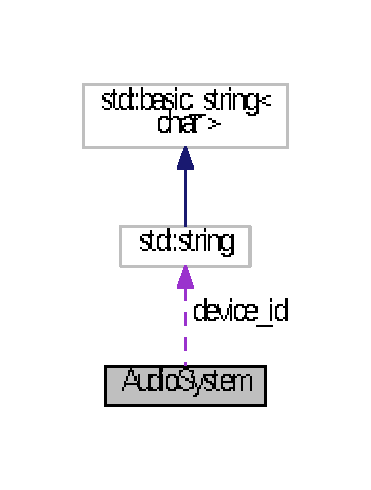
\includegraphics[width=178pt]{classAudioSystem__coll__graph}
\end{center}
\end{figure}
\subsection*{Public Types}
\begin{DoxyCompactItemize}
\item 
\hypertarget{classAudioSystem_a33bfa767bca10a6ce71e72708c586c67}{using \hyperlink{classAudioSystem_a33bfa767bca10a6ce71e72708c586c67}{Device} = std\+::pair$<$ int, std\+::string $>$}\label{classAudioSystem_a33bfa767bca10a6ce71e72708c586c67}

\begin{DoxyCompactList}\small\item\em Type for device entries. \end{DoxyCompactList}\end{DoxyCompactItemize}
\subsection*{Public Member Functions}
\begin{DoxyCompactItemize}
\item 
\hyperlink{classAudioSystem_ad17cde8deff07ef7d7d56be62df98739}{Audio\+System} ()
\begin{DoxyCompactList}\small\item\em Constructs an \hyperlink{classAudioSystem}{Audio\+System}, initialising its libraries. \end{DoxyCompactList}\item 
\hypertarget{classAudioSystem_a9ad830040ea5f68a6a63957c6f281055}{\hyperlink{classAudioSystem_a9ad830040ea5f68a6a63957c6f281055}{$\sim$\+Audio\+System} ()}\label{classAudioSystem_a9ad830040ea5f68a6a63957c6f281055}

\begin{DoxyCompactList}\small\item\em Destructs an \hyperlink{classAudioSystem}{Audio\+System}, uninitialising its libraries. \end{DoxyCompactList}\item 
\hyperlink{classAudio}{Audio} $\ast$ \hyperlink{classAudioSystem_a2172608177d2bd54377bfc3c61cd117d}{Load} (const std\+::string \&path) const 
\begin{DoxyCompactList}\small\item\em Loads a file, creating an \hyperlink{classAudio}{Audio} for it. \end{DoxyCompactList}\item 
void \hyperlink{classAudioSystem_ade3b400828991d02e36a0b61302d30d2}{Set\+Device\+I\+D} (int id)
\begin{DoxyCompactList}\small\item\em Sets the current device I\+D. \end{DoxyCompactList}\item 
std\+::vector$<$ \hyperlink{classAudioSystem_a33bfa767bca10a6ce71e72708c586c67}{Audio\+System\+::\+Device} $>$ \hyperlink{classAudioSystem_aa268faeb9243c18588631024958856e6}{Get\+Devices\+Info} ()
\begin{DoxyCompactList}\small\item\em Gets the number and name of each output device entry in the \hyperlink{classAudioSystem}{Audio\+System}. \end{DoxyCompactList}\item 
bool \hyperlink{classAudioSystem_a001cd82f854883b80b3ed7d35795581b}{Is\+Output\+Device} (int id)
\begin{DoxyCompactList}\small\item\em Can a sound device output sound? \end{DoxyCompactList}\item 
portaudio\+::\+Stream $\ast$ \hyperlink{classAudioSystem_a78e8754440e0a29f5fac9ca1cd79a109}{Configure} (std\+::uint8\+\_\+t channel\+\_\+count, \hyperlink{sample__formats_8hpp_a21cca244e782ff3acc8805fb73236772}{Sample\+Format} sample\+\_\+format, double sample\+\_\+rate, size\+\_\+t buffer\+\_\+size, portaudio\+::\+Callback\+Interface \&cb) const 
\begin{DoxyCompactList}\small\item\em Configures and returns a Port\+Audio stream. \end{DoxyCompactList}\end{DoxyCompactItemize}
\subsection*{Private Member Functions}
\begin{DoxyCompactItemize}
\item 
const portaudio\+::\+Device \& \hyperlink{classAudioSystem_a513a0de4748574e25cba443f28949a90}{Pa\+Device\+From} (const std\+::string \&id\+\_\+string) const 
\begin{DoxyCompactList}\small\item\em Converts a string device I\+D to a Port\+Audio device. \end{DoxyCompactList}\item 
portaudio\+::\+Sample\+Data\+Format \hyperlink{classAudioSystem_aac640b14ad80c2518539bcafe9f4b5ac}{Pa\+Sample\+Format\+From} (\hyperlink{sample__formats_8hpp_a21cca244e782ff3acc8805fb73236772}{Sample\+Format} fmt) const 
\begin{DoxyCompactList}\small\item\em Converts a sample format identifier from playd to Port\+Audio. \end{DoxyCompactList}\end{DoxyCompactItemize}
\subsection*{Private Attributes}
\begin{DoxyCompactItemize}
\item 
\hypertarget{classAudioSystem_a3071e6d8643b3d0275ba63820e6e0072}{std\+::string \hyperlink{classAudioSystem_a3071e6d8643b3d0275ba63820e6e0072}{device\+\_\+id}}\label{classAudioSystem_a3071e6d8643b3d0275ba63820e6e0072}

\begin{DoxyCompactList}\small\item\em The current device I\+D. \end{DoxyCompactList}\end{DoxyCompactItemize}


\subsection{Detailed Description}
An \hyperlink{classAudioSystem}{Audio\+System} represents the entire audio stack used by playd. 

The \hyperlink{classAudioSystem}{Audio\+System} is responsible for creating \hyperlink{classAudio}{Audio} instances, enumerating and resolving device I\+Ds, and initialising and terminating the audio libraries.

\hyperlink{classAudioSystem}{Audio\+System} is a R\+A\+I\+I-\/style class\+: it loads the audio libraries on construction and unloads them on termination. As such, it's probably not wise to construct multiple \hyperlink{classAudioSystem}{Audio\+System} instances. 

Definition at line \hyperlink{audio__system_8hpp_source_l00040}{40} of file \hyperlink{audio__system_8hpp_source}{audio\+\_\+system.\+hpp}.



\subsection{Constructor \& Destructor Documentation}
\hypertarget{classAudioSystem_ad17cde8deff07ef7d7d56be62df98739}{\index{Audio\+System@{Audio\+System}!Audio\+System@{Audio\+System}}
\index{Audio\+System@{Audio\+System}!Audio\+System@{Audio\+System}}
\subsubsection[{Audio\+System}]{\setlength{\rightskip}{0pt plus 5cm}Audio\+System\+::\+Audio\+System (
\begin{DoxyParamCaption}
{}
\end{DoxyParamCaption}
)}}\label{classAudioSystem_ad17cde8deff07ef7d7d56be62df98739}


Constructs an \hyperlink{classAudioSystem}{Audio\+System}, initialising its libraries. 

This sets the current device I\+D to a sane default; use Set\+Device\+I\+D to change it. 

Definition at line \hyperlink{audio__system_8cpp_source_l00041}{41} of file \hyperlink{audio__system_8cpp_source}{audio\+\_\+system.\+cpp}.



References \hyperlink{audio__system_8hpp_source_l00101}{device\+\_\+id}.


\begin{DoxyCode}
00042 \{
00043     portaudio::System::initialize();
00044     sox\_format\_init();
00045 
00046     this->\hyperlink{classAudioSystem_a3071e6d8643b3d0275ba63820e6e0072}{device\_id} = -1;
00047 \}
\end{DoxyCode}


\subsection{Member Function Documentation}
\hypertarget{classAudioSystem_a78e8754440e0a29f5fac9ca1cd79a109}{\index{Audio\+System@{Audio\+System}!Configure@{Configure}}
\index{Configure@{Configure}!Audio\+System@{Audio\+System}}
\subsubsection[{Configure}]{\setlength{\rightskip}{0pt plus 5cm}portaudio\+::\+Stream $\ast$ Audio\+System\+::\+Configure (
\begin{DoxyParamCaption}
\item[{std\+::uint8\+\_\+t}]{channel\+\_\+count, }
\item[{{\bf Sample\+Format}}]{sample\+\_\+format, }
\item[{double}]{sample\+\_\+rate, }
\item[{size\+\_\+t}]{buffer\+\_\+size, }
\item[{portaudio\+::\+Callback\+Interface \&}]{cb}
\end{DoxyParamCaption}
) const}}\label{classAudioSystem_a78e8754440e0a29f5fac9ca1cd79a109}


Configures and returns a Port\+Audio stream. 


\begin{DoxyParams}{Parameters}
{\em channel\+\_\+count} & The number of channels of the stream will receive. \\
\hline
{\em sample\+\_\+format} & The format of the samples the stream will receive. \\
\hline
{\em sample\+\_\+rate} & The rate of the samples the stream will receive. \\
\hline
{\em buffer\+\_\+size} & The size of the buffer the stream should allocate. \\
\hline
{\em cb} & The object that Port\+Audio will call to receive audio. \\
\hline
\end{DoxyParams}
\begin{DoxyReturn}{Returns}
The configured Port\+Audio stream. 
\end{DoxyReturn}


Definition at line \hyperlink{audio__system_8cpp_source_l00096}{96} of file \hyperlink{audio__system_8cpp_source}{audio\+\_\+system.\+cpp}.



References \hyperlink{audio__system_8hpp_source_l00101}{device\+\_\+id}, \hyperlink{audio__system_8cpp_source_l00115}{Pa\+Device\+From()}, and \hyperlink{audio__system_8cpp_source_l00140}{Pa\+Sample\+Format\+From()}.



Referenced by \hyperlink{audio__system_8cpp_source_l00083}{Load()}.


\begin{DoxyCode}
00100 \{
00101     \textcolor{keyword}{const} portaudio::Device &device = \hyperlink{classAudioSystem_a513a0de4748574e25cba443f28949a90}{PaDeviceFrom}(this->\hyperlink{classAudioSystem_a3071e6d8643b3d0275ba63820e6e0072}{device\_id});
00102 
00103     portaudio::DirectionSpecificStreamParameters out\_pars(
00104                     device, channel\_count,
00105                     \hyperlink{classAudioSystem_aac640b14ad80c2518539bcafe9f4b5ac}{PaSampleFormatFrom}(sample\_format), \textcolor{keyword}{true},
00106                     device.defaultLowOutputLatency(), \textcolor{keyword}{nullptr});
00107 
00108     portaudio::StreamParameters pars(
00109                     portaudio::DirectionSpecificStreamParameters::null(),
00110                     out\_pars, sample\_rate, buffer\_size, paClipOff);
00111 
00112     \textcolor{keywordflow}{return} \textcolor{keyword}{new} portaudio::InterfaceCallbackStream(pars, cb);
00113 \}
\end{DoxyCode}
\hypertarget{classAudioSystem_aa268faeb9243c18588631024958856e6}{\index{Audio\+System@{Audio\+System}!Get\+Devices\+Info@{Get\+Devices\+Info}}
\index{Get\+Devices\+Info@{Get\+Devices\+Info}!Audio\+System@{Audio\+System}}
\subsubsection[{Get\+Devices\+Info}]{\setlength{\rightskip}{0pt plus 5cm}std\+::vector$<$ {\bf Audio\+System\+::\+Device} $>$ Audio\+System\+::\+Get\+Devices\+Info (
\begin{DoxyParamCaption}
{}
\end{DoxyParamCaption}
)}}\label{classAudioSystem_aa268faeb9243c18588631024958856e6}


Gets the number and name of each output device entry in the \hyperlink{classAudioSystem}{Audio\+System}. 

\begin{DoxyReturn}{Returns}
List of output devices, as strings. 
\end{DoxyReturn}


Definition at line \hyperlink{audio__system_8cpp_source_l00055}{55} of file \hyperlink{audio__system_8cpp_source}{audio\+\_\+system.\+cpp}.



Referenced by \hyperlink{main_8cpp_source_l00040}{playd\+::\+Get\+Device\+I\+D()}, and \hyperlink{main_8cpp_source_l00130}{playd\+::\+Run()}.


\begin{DoxyCode}
00056 \{
00057     \textcolor{keyword}{auto} &pa = portaudio::System::instance();
00058     std::vector<AudioSystem::Device> list;
00059 
00060     \textcolor{keywordflow}{for} (\textcolor{keyword}{auto} d = pa.devicesBegin(); d != pa.devicesEnd(); ++d) \{
00061         \textcolor{keywordflow}{if} (!(*d).isInputOnlyDevice()) \{
00062             list.push\_back(std::make\_pair((*d).index(),
00063                                           (*d).name()));
00064         \}
00065     \}
00066     \textcolor{keywordflow}{return} list;
00067 \}
\end{DoxyCode}
\hypertarget{classAudioSystem_a001cd82f854883b80b3ed7d35795581b}{\index{Audio\+System@{Audio\+System}!Is\+Output\+Device@{Is\+Output\+Device}}
\index{Is\+Output\+Device@{Is\+Output\+Device}!Audio\+System@{Audio\+System}}
\subsubsection[{Is\+Output\+Device}]{\setlength{\rightskip}{0pt plus 5cm}bool Audio\+System\+::\+Is\+Output\+Device (
\begin{DoxyParamCaption}
\item[{int}]{id}
\end{DoxyParamCaption}
)}}\label{classAudioSystem_a001cd82f854883b80b3ed7d35795581b}


Can a sound device output sound? 


\begin{DoxyParams}{Parameters}
{\em id} & Device I\+D. \\
\hline
\end{DoxyParams}
\begin{DoxyReturn}{Returns}
If the device can handle outputting sound. 
\end{DoxyReturn}


Definition at line \hyperlink{audio__system_8cpp_source_l00069}{69} of file \hyperlink{audio__system_8cpp_source}{audio\+\_\+system.\+cpp}.



Referenced by \hyperlink{main_8cpp_source_l00040}{playd\+::\+Get\+Device\+I\+D()}.


\begin{DoxyCode}
00070 \{
00071     \textcolor{keyword}{auto} &pa = portaudio::System::instance();
00072     \textcolor{keywordflow}{if} (id < 0 || id >= pa.deviceCount()) \textcolor{keywordflow}{return} \textcolor{keyword}{false};
00073 
00074     portaudio::Device &dev = pa.deviceByIndex(\textcolor{keywordtype}{id});
00075     \textcolor{keywordflow}{return} !dev.isInputOnlyDevice();
00076 \}
\end{DoxyCode}
\hypertarget{classAudioSystem_a2172608177d2bd54377bfc3c61cd117d}{\index{Audio\+System@{Audio\+System}!Load@{Load}}
\index{Load@{Load}!Audio\+System@{Audio\+System}}
\subsubsection[{Load}]{\setlength{\rightskip}{0pt plus 5cm}{\bf Audio} $\ast$ Audio\+System\+::\+Load (
\begin{DoxyParamCaption}
\item[{const std\+::string \&}]{path}
\end{DoxyParamCaption}
) const}}\label{classAudioSystem_a2172608177d2bd54377bfc3c61cd117d}


Loads a file, creating an \hyperlink{classAudio}{Audio} for it. 


\begin{DoxyParams}{Parameters}
{\em path} & The path to a file. \\
\hline
\end{DoxyParams}
\begin{DoxyReturn}{Returns}
The \hyperlink{classAudio}{Audio} for that file. 
\end{DoxyReturn}


Definition at line \hyperlink{audio__system_8cpp_source_l00083}{83} of file \hyperlink{audio__system_8cpp_source}{audio\+\_\+system.\+cpp}.



References \hyperlink{audio__system_8cpp_source_l00096}{Configure()}.



Referenced by \hyperlink{player__file_8cpp_source_l00025}{Player\+File\+::\+Load()}.


\begin{DoxyCode}
00084 \{
00085     \textcolor{keyword}{auto} source = \textcolor{keyword}{new} \hyperlink{classAudioSource}{AudioSource}(path);
00086 
00087     \hyperlink{classAudioSink_ae5b8370aa17c24c6fc8f8e0c5778168c}{AudioSink::StreamConfigurator} config\_fn = std::bind(
00088                     &\hyperlink{classAudioSystem_a78e8754440e0a29f5fac9ca1cd79a109}{AudioSystem::Configure}, \textcolor{keyword}{this}, source->ChannelCount(),
00089                     source->OutputSampleFormat(), source->SampleRate(),
00090                     source->BufferSampleCapacity(), std::placeholders::\_1);
00091     \textcolor{keyword}{auto} sink = \textcolor{keyword}{new} \hyperlink{classAudioSink}{AudioSink}(config\_fn, source->BytesPerSample());
00092 
00093     \textcolor{keywordflow}{return} \textcolor{keyword}{new} \hyperlink{classAudio}{Audio}(source, sink);
00094 \}
\end{DoxyCode}
\hypertarget{classAudioSystem_a513a0de4748574e25cba443f28949a90}{\index{Audio\+System@{Audio\+System}!Pa\+Device\+From@{Pa\+Device\+From}}
\index{Pa\+Device\+From@{Pa\+Device\+From}!Audio\+System@{Audio\+System}}
\subsubsection[{Pa\+Device\+From}]{\setlength{\rightskip}{0pt plus 5cm}const portaudio\+::\+Device \& Audio\+System\+::\+Pa\+Device\+From (
\begin{DoxyParamCaption}
\item[{const std\+::string \&}]{id\+\_\+string}
\end{DoxyParamCaption}
) const\hspace{0.3cm}{\ttfamily [private]}}}\label{classAudioSystem_a513a0de4748574e25cba443f28949a90}


Converts a string device I\+D to a Port\+Audio device. 


\begin{DoxyParams}{Parameters}
{\em id\+\_\+string} & The device I\+D, as a string. \\
\hline
\end{DoxyParams}
\begin{DoxyReturn}{Returns}
The device. 
\end{DoxyReturn}


Definition at line \hyperlink{audio__system_8cpp_source_l00115}{115} of file \hyperlink{audio__system_8cpp_source}{audio\+\_\+system.\+cpp}.



References \hyperlink{messages_8h_source_l00036}{M\+S\+G\+\_\+\+D\+E\+V\+\_\+\+B\+A\+D\+I\+D}.



Referenced by \hyperlink{audio__system_8cpp_source_l00096}{Configure()}.


\begin{DoxyCode}
00117 \{
00118     \textcolor{keyword}{auto} &pa = portaudio::System::instance();
00119 
00120     PaDeviceIndex id\_pa = 0;
00121 
00122     std::istringstream is(id\_string);
00123     is >> id\_pa;
00124 
00125     \textcolor{keywordflow}{if} (id\_pa >= pa.deviceCount()) \{
00126         \textcolor{keywordflow}{throw} \hyperlink{classConfigError}{ConfigError}(\hyperlink{messages_8h_a80a8cb0d00a63114c8c5c8228fa39ec4}{MSG\_DEV\_BADID});
00127     \}
00128 
00129     \textcolor{keywordflow}{return} pa.deviceByIndex(id\_pa);
00130 \}
\end{DoxyCode}
\hypertarget{classAudioSystem_aac640b14ad80c2518539bcafe9f4b5ac}{\index{Audio\+System@{Audio\+System}!Pa\+Sample\+Format\+From@{Pa\+Sample\+Format\+From}}
\index{Pa\+Sample\+Format\+From@{Pa\+Sample\+Format\+From}!Audio\+System@{Audio\+System}}
\subsubsection[{Pa\+Sample\+Format\+From}]{\setlength{\rightskip}{0pt plus 5cm}portaudio\+::\+Sample\+Data\+Format Audio\+System\+::\+Pa\+Sample\+Format\+From (
\begin{DoxyParamCaption}
\item[{{\bf Sample\+Format}}]{fmt}
\end{DoxyParamCaption}
) const\hspace{0.3cm}{\ttfamily [private]}}}\label{classAudioSystem_aac640b14ad80c2518539bcafe9f4b5ac}


Converts a sample format identifier from playd to Port\+Audio. 


\begin{DoxyParams}{Parameters}
{\em fmt} & The playd sample format identifier. \\
\hline
\end{DoxyParams}
\begin{DoxyReturn}{Returns}
The Port\+Audio equivalent of the given Sample\+Format. 
\end{DoxyReturn}


Definition at line \hyperlink{audio__system_8cpp_source_l00140}{140} of file \hyperlink{audio__system_8cpp_source}{audio\+\_\+system.\+cpp}.



References \hyperlink{messages_8h_source_l00030}{M\+S\+G\+\_\+\+D\+E\+C\+O\+D\+E\+\_\+\+B\+A\+D\+R\+A\+T\+E}.



Referenced by \hyperlink{audio__system_8cpp_source_l00096}{Configure()}.


\begin{DoxyCode}
00142 \{
00143     \textcolor{keywordflow}{try}
00144     \{
00145         \textcolor{keywordflow}{return} pa\_from\_sf.at(fmt);
00146     \}
00147     \textcolor{keywordflow}{catch} (std::out\_of\_range)
00148     \{
00149         \textcolor{keywordflow}{throw} \hyperlink{classFileError}{FileError}(\hyperlink{messages_8h_a6d4302117e822520f5c61b6d40085c4d}{MSG\_DECODE\_BADRATE});
00150     \}
00151 \}
\end{DoxyCode}
\hypertarget{classAudioSystem_ade3b400828991d02e36a0b61302d30d2}{\index{Audio\+System@{Audio\+System}!Set\+Device\+I\+D@{Set\+Device\+I\+D}}
\index{Set\+Device\+I\+D@{Set\+Device\+I\+D}!Audio\+System@{Audio\+System}}
\subsubsection[{Set\+Device\+I\+D}]{\setlength{\rightskip}{0pt plus 5cm}void Audio\+System\+::\+Set\+Device\+I\+D (
\begin{DoxyParamCaption}
\item[{int}]{id}
\end{DoxyParamCaption}
)}}\label{classAudioSystem_ade3b400828991d02e36a0b61302d30d2}


Sets the current device I\+D. 


\begin{DoxyParams}{Parameters}
{\em id} & The device I\+D to use for subsequent Audios. \\
\hline
\end{DoxyParams}


Definition at line \hyperlink{audio__system_8cpp_source_l00078}{78} of file \hyperlink{audio__system_8cpp_source}{audio\+\_\+system.\+cpp}.



References \hyperlink{audio__system_8hpp_source_l00101}{device\+\_\+id}.



Referenced by \hyperlink{main_8cpp_source_l00130}{playd\+::\+Run()}.


\begin{DoxyCode}
00079 \{
00080     this->\hyperlink{classAudioSystem_a3071e6d8643b3d0275ba63820e6e0072}{device\_id} = std::to\_string(\textcolor{keywordtype}{id});
00081 \}
\end{DoxyCode}


The documentation for this class was generated from the following files\+:\begin{DoxyCompactItemize}
\item 
src/audio/\hyperlink{audio__system_8hpp}{audio\+\_\+system.\+hpp}\item 
src/audio/\hyperlink{audio__system_8cpp}{audio\+\_\+system.\+cpp}\end{DoxyCompactItemize}

\hypertarget{classCommandHandler}{\section{Command\+Handler Class Reference}
\label{classCommandHandler}\index{Command\+Handler@{Command\+Handler}}
}


The playd command handler.  




{\ttfamily \#include $<$cmd.\+hpp$>$}



Collaboration diagram for Command\+Handler\+:
\nopagebreak
\begin{figure}[H]
\begin{center}
\leavevmode
\includegraphics[width=350pt]{classCommandHandler__coll__graph}
\end{center}
\end{figure}
\subsection*{Public Types}
\begin{DoxyCompactItemize}
\item 
\hypertarget{classCommandHandler_ae6cc650f171966041b385c8a4a766639}{using \hyperlink{classCommandHandler_ae6cc650f171966041b385c8a4a766639}{Word\+List} = std\+::vector$<$ std\+::string $>$}\label{classCommandHandler_ae6cc650f171966041b385c8a4a766639}

\begin{DoxyCompactList}\small\item\em The type of lists of command words. \end{DoxyCompactList}\end{DoxyCompactItemize}
\subsection*{Public Member Functions}
\begin{DoxyCompactItemize}
\item 
\hyperlink{classCommandHandler_ae4d47b90e2cf2ab6d514576fedeb2192}{Command\+Handler} (\hyperlink{classPlayer}{Player} \&\hyperlink{classCommandHandler_a398ba97a0625f5fbc3ced6679cfd3766}{player})
\begin{DoxyCompactList}\small\item\em Constructs a \hyperlink{classCommandHandler}{Command\+Handler}. \end{DoxyCompactList}\item 
bool \hyperlink{classCommandHandler_abc1ad0dfbff50db168d0a65cf05b169e}{Handle} (const \hyperlink{classCommandHandler_ae6cc650f171966041b385c8a4a766639}{Word\+List} \&words)
\begin{DoxyCompactList}\small\item\em Handles a command line. \end{DoxyCompactList}\end{DoxyCompactItemize}
\subsection*{Private Member Functions}
\begin{DoxyCompactItemize}
\item 
bool \hyperlink{classCommandHandler_a22ac65683643c6f6037441a8e5fd04d4}{Run\+Nullary} (const std\+::string \&cmd)
\begin{DoxyCompactList}\small\item\em Runs a nullary (0-\/argument) command. \end{DoxyCompactList}\item 
bool \hyperlink{classCommandHandler_a75904aa3532bba1e548fbcff00544d46}{Run\+Unary} (const std\+::string \&cmd, const std\+::string \&arg)
\begin{DoxyCompactList}\small\item\em Runs a unary (1-\/argument) command. \end{DoxyCompactList}\end{DoxyCompactItemize}
\subsection*{Private Attributes}
\begin{DoxyCompactItemize}
\item 
\hypertarget{classCommandHandler_a398ba97a0625f5fbc3ced6679cfd3766}{\hyperlink{classPlayer}{Player} \& \hyperlink{classCommandHandler_a398ba97a0625f5fbc3ced6679cfd3766}{player}}\label{classCommandHandler_a398ba97a0625f5fbc3ced6679cfd3766}

\begin{DoxyCompactList}\small\item\em Reference to the \hyperlink{classPlayer}{Player} on which commands run. \end{DoxyCompactList}\end{DoxyCompactItemize}


\subsection{Detailed Description}
The playd command handler. 

Definition at line \hyperlink{cmd_8hpp_source_l00027}{27} of file \hyperlink{cmd_8hpp_source}{cmd.\+hpp}.



\subsection{Constructor \& Destructor Documentation}
\hypertarget{classCommandHandler_ae4d47b90e2cf2ab6d514576fedeb2192}{\index{Command\+Handler@{Command\+Handler}!Command\+Handler@{Command\+Handler}}
\index{Command\+Handler@{Command\+Handler}!Command\+Handler@{Command\+Handler}}
\subsubsection[{Command\+Handler}]{\setlength{\rightskip}{0pt plus 5cm}Command\+Handler\+::\+Command\+Handler (
\begin{DoxyParamCaption}
\item[{{\bf Player} \&}]{player}
\end{DoxyParamCaption}
)}}\label{classCommandHandler_ae4d47b90e2cf2ab6d514576fedeb2192}


Constructs a \hyperlink{classCommandHandler}{Command\+Handler}. 


\begin{DoxyParams}{Parameters}
{\em player} & A reference to the \hyperlink{classPlayer}{Player} on which the playd commands will run. \\
\hline
\end{DoxyParams}


Definition at line \hyperlink{cmd_8cpp_source_l00018}{18} of file \hyperlink{cmd_8cpp_source}{cmd.\+cpp}.


\begin{DoxyCode}
00018                                              : \hyperlink{classCommandHandler_a398ba97a0625f5fbc3ced6679cfd3766}{player}(player)
00019 \{
00020 \}
\end{DoxyCode}


\subsection{Member Function Documentation}
\hypertarget{classCommandHandler_abc1ad0dfbff50db168d0a65cf05b169e}{\index{Command\+Handler@{Command\+Handler}!Handle@{Handle}}
\index{Handle@{Handle}!Command\+Handler@{Command\+Handler}}
\subsubsection[{Handle}]{\setlength{\rightskip}{0pt plus 5cm}bool Command\+Handler\+::\+Handle (
\begin{DoxyParamCaption}
\item[{const {\bf Word\+List} \&}]{words}
\end{DoxyParamCaption}
)}}\label{classCommandHandler_abc1ad0dfbff50db168d0a65cf05b169e}


Handles a command line. 


\begin{DoxyParams}{Parameters}
{\em words} & A reference to the list of words in the command. \\
\hline
\end{DoxyParams}
\begin{DoxyReturn}{Returns}
Whether the command succeeded. 
\end{DoxyReturn}


Definition at line \hyperlink{cmd_8cpp_source_l00022}{22} of file \hyperlink{cmd_8cpp_source}{cmd.\+cpp}.



References \hyperlink{cmd_8cpp_source_l00032}{Run\+Nullary()}, and \hyperlink{cmd_8cpp_source_l00041}{Run\+Unary()}.



Referenced by \hyperlink{tokeniser_8cpp_source_l00113}{Tokeniser\+::\+Emit()}.


\begin{DoxyCode}
00023 \{
00024     \textcolor{keywordflow}{if} (words.size() == 1) \{
00025         \textcolor{keywordflow}{return} \hyperlink{classCommandHandler_a22ac65683643c6f6037441a8e5fd04d4}{RunNullary}(words[0]);
00026     \} \textcolor{keywordflow}{else} \textcolor{keywordflow}{if} (words.size() == 2 && !words[1].empty()) \{
00027         \textcolor{keywordflow}{return} \hyperlink{classCommandHandler_a75904aa3532bba1e548fbcff00544d46}{RunUnary}(words[0], words[1]);
00028     \}
00029     \textcolor{keywordflow}{return} \textcolor{keyword}{false};
00030 \}
\end{DoxyCode}
\hypertarget{classCommandHandler_a22ac65683643c6f6037441a8e5fd04d4}{\index{Command\+Handler@{Command\+Handler}!Run\+Nullary@{Run\+Nullary}}
\index{Run\+Nullary@{Run\+Nullary}!Command\+Handler@{Command\+Handler}}
\subsubsection[{Run\+Nullary}]{\setlength{\rightskip}{0pt plus 5cm}bool Command\+Handler\+::\+Run\+Nullary (
\begin{DoxyParamCaption}
\item[{const std\+::string \&}]{cmd}
\end{DoxyParamCaption}
)\hspace{0.3cm}{\ttfamily [private]}}}\label{classCommandHandler_a22ac65683643c6f6037441a8e5fd04d4}


Runs a nullary (0-\/argument) command. 


\begin{DoxyParams}{Parameters}
{\em cmd} & The command word. \\
\hline
\end{DoxyParams}
\begin{DoxyReturn}{Returns}
True if the command was successfully found and executed; false otherwise. 
\end{DoxyReturn}
\begin{DoxyRefDesc}{Todo}
\item[\hyperlink{todo__todo000001}{Todo}]Richer command results. \end{DoxyRefDesc}


Definition at line \hyperlink{cmd_8cpp_source_l00032}{32} of file \hyperlink{cmd_8cpp_source}{cmd.\+cpp}.



References \hyperlink{player_8cpp_source_l00079}{Player\+::\+Eject()}, \hyperlink{player_8cpp_source_l00116}{Player\+::\+Play()}, \hyperlink{cmd_8hpp_source_l00048}{player}, \hyperlink{player_8cpp_source_l00126}{Player\+::\+Quit()}, and \hyperlink{player_8cpp_source_l00159}{Player\+::\+Stop()}.



Referenced by \hyperlink{cmd_8cpp_source_l00022}{Handle()}.


\begin{DoxyCode}
00033 \{
00034     \textcolor{keywordflow}{if} (\textcolor{stringliteral}{"play"} == cmd) \textcolor{keywordflow}{return} this->\hyperlink{classCommandHandler_a398ba97a0625f5fbc3ced6679cfd3766}{player}.\hyperlink{classPlayer_a1df3950102f682608482042cdea96598}{Play}();
00035     \textcolor{keywordflow}{if} (\textcolor{stringliteral}{"stop"} == cmd) \textcolor{keywordflow}{return} this->\hyperlink{classCommandHandler_a398ba97a0625f5fbc3ced6679cfd3766}{player}.\hyperlink{classPlayer_abe074115b0ffa631ea432a1b84171599}{Stop}();
00036     \textcolor{keywordflow}{if} (\textcolor{stringliteral}{"eject"} == cmd) \textcolor{keywordflow}{return} this->\hyperlink{classCommandHandler_a398ba97a0625f5fbc3ced6679cfd3766}{player}.\hyperlink{classPlayer_ac93a5310c751e8a9221780933f7a9dd6}{Eject}();
00037     \textcolor{keywordflow}{if} (\textcolor{stringliteral}{"quit"} == cmd) \textcolor{keywordflow}{return} this->\hyperlink{classCommandHandler_a398ba97a0625f5fbc3ced6679cfd3766}{player}.\hyperlink{classPlayer_a7d5c0535d543b358b6deecb054565b97}{Quit}();
00038     \textcolor{keywordflow}{return} \textcolor{keyword}{false};
00039 \}
\end{DoxyCode}
\hypertarget{classCommandHandler_a75904aa3532bba1e548fbcff00544d46}{\index{Command\+Handler@{Command\+Handler}!Run\+Unary@{Run\+Unary}}
\index{Run\+Unary@{Run\+Unary}!Command\+Handler@{Command\+Handler}}
\subsubsection[{Run\+Unary}]{\setlength{\rightskip}{0pt plus 5cm}bool Command\+Handler\+::\+Run\+Unary (
\begin{DoxyParamCaption}
\item[{const std\+::string \&}]{cmd, }
\item[{const std\+::string \&}]{arg}
\end{DoxyParamCaption}
)\hspace{0.3cm}{\ttfamily [private]}}}\label{classCommandHandler_a75904aa3532bba1e548fbcff00544d46}


Runs a unary (1-\/argument) command. 


\begin{DoxyParams}{Parameters}
{\em cmd} & The command word. \\
\hline
{\em arg} & The argument to the command. \\
\hline
\end{DoxyParams}
\begin{DoxyReturn}{Returns}
True if the command was successfully found and executed; false otherwise. 
\end{DoxyReturn}
\begin{DoxyRefDesc}{Todo}
\item[\hyperlink{todo__todo000002}{Todo}]Richer command results. \end{DoxyRefDesc}


Definition at line \hyperlink{cmd_8cpp_source_l00041}{41} of file \hyperlink{cmd_8cpp_source}{cmd.\+cpp}.



References \hyperlink{player_8cpp_source_l00089}{Player\+::\+Load()}, \hyperlink{cmd_8hpp_source_l00048}{player}, and \hyperlink{player_8cpp_source_l00134}{Player\+::\+Seek()}.



Referenced by \hyperlink{cmd_8cpp_source_l00022}{Handle()}.


\begin{DoxyCode}
00042 \{
00043     \textcolor{keywordflow}{if} (\textcolor{stringliteral}{"load"} == cmd) \textcolor{keywordflow}{return} this->\hyperlink{classCommandHandler_a398ba97a0625f5fbc3ced6679cfd3766}{player}.\hyperlink{classPlayer_a41c5eccb1f3b86383eaafe56a40a60e0}{Load}(arg);
00044     \textcolor{keywordflow}{if} (\textcolor{stringliteral}{"seek"} == cmd) \textcolor{keywordflow}{return} this->\hyperlink{classCommandHandler_a398ba97a0625f5fbc3ced6679cfd3766}{player}.\hyperlink{classPlayer_a873c7e0a5be71efbadeebfbc20d7448a}{Seek}(arg);
00045     \textcolor{keywordflow}{return} \textcolor{keyword}{false};
00046 \}
\end{DoxyCode}


The documentation for this class was generated from the following files\+:\begin{DoxyCompactItemize}
\item 
src/\hyperlink{cmd_8hpp}{cmd.\+hpp}\item 
src/\hyperlink{cmd_8cpp}{cmd.\+cpp}\end{DoxyCompactItemize}

\hypertarget{classConfigError}{\section{Config\+Error Class Reference}
\label{classConfigError}\index{Config\+Error@{Config\+Error}}
}


An \hyperlink{classError}{Error} signifying that playd has been improperly configured.  




{\ttfamily \#include $<$errors.\+hpp$>$}



Inheritance diagram for Config\+Error\+:
\nopagebreak
\begin{figure}[H]
\begin{center}
\leavevmode
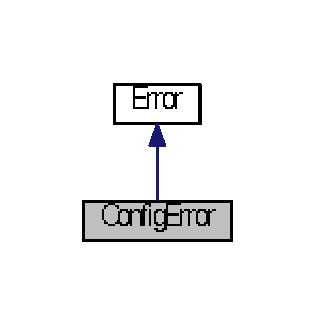
\includegraphics[width=151pt]{classConfigError__inherit__graph}
\end{center}
\end{figure}


Collaboration diagram for Config\+Error\+:
\nopagebreak
\begin{figure}[H]
\begin{center}
\leavevmode
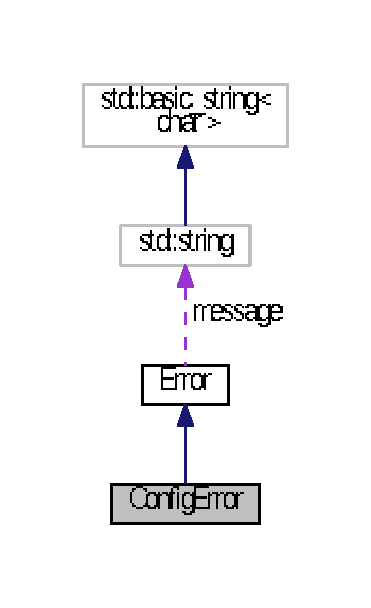
\includegraphics[width=178pt]{classConfigError__coll__graph}
\end{center}
\end{figure}
\subsection*{Public Member Functions}
\begin{DoxyCompactItemize}
\item 
\hyperlink{classConfigError_a0df38d0770d8e8299e628793058bb2eb}{Config\+Error} (const std\+::string \&\hyperlink{classError_aa4713ef3ee9c3c0da43a54b01949510d}{message})
\begin{DoxyCompactList}\small\item\em Constructs an \hyperlink{classConfigError}{Config\+Error}. \end{DoxyCompactList}\end{DoxyCompactItemize}


\subsection{Detailed Description}
An \hyperlink{classError}{Error} signifying that playd has been improperly configured. 

Definition at line \hyperlink{errors_8hpp_source_l00044}{44} of file \hyperlink{errors_8hpp_source}{errors.\+hpp}.



\subsection{Constructor \& Destructor Documentation}
\hypertarget{classConfigError_a0df38d0770d8e8299e628793058bb2eb}{\index{Config\+Error@{Config\+Error}!Config\+Error@{Config\+Error}}
\index{Config\+Error@{Config\+Error}!Config\+Error@{Config\+Error}}
\subsubsection[{Config\+Error}]{\setlength{\rightskip}{0pt plus 5cm}Config\+Error\+::\+Config\+Error (
\begin{DoxyParamCaption}
\item[{const std\+::string \&}]{message}
\end{DoxyParamCaption}
)\hspace{0.3cm}{\ttfamily [inline]}}}\label{classConfigError_a0df38d0770d8e8299e628793058bb2eb}


Constructs an \hyperlink{classConfigError}{Config\+Error}. 


\begin{DoxyParams}{Parameters}
{\em message} & The human-\/readable message of the error. \\
\hline
\end{DoxyParams}


Definition at line \hyperlink{errors_8hpp_source_l00050}{50} of file \hyperlink{errors_8hpp_source}{errors.\+hpp}.


\begin{DoxyCode}
00050 : \hyperlink{classError_accd611f3ddae0828adeb6ca251113ffd}{Error}(\hyperlink{classError_aa4713ef3ee9c3c0da43a54b01949510d}{message}) \{\};
\end{DoxyCode}


The documentation for this class was generated from the following file\+:\begin{DoxyCompactItemize}
\item 
src/\hyperlink{errors_8hpp}{errors.\+hpp}\end{DoxyCompactItemize}

\hypertarget{classDebug}{\section{Debug Class Reference}
\label{classDebug}\index{Debug@{Debug}}
}


Class for telling the human what playd is doing.  




{\ttfamily \#include $<$errors.\+hpp$>$}



Collaboration diagram for Debug\+:
\nopagebreak
\begin{figure}[H]
\begin{center}
\leavevmode
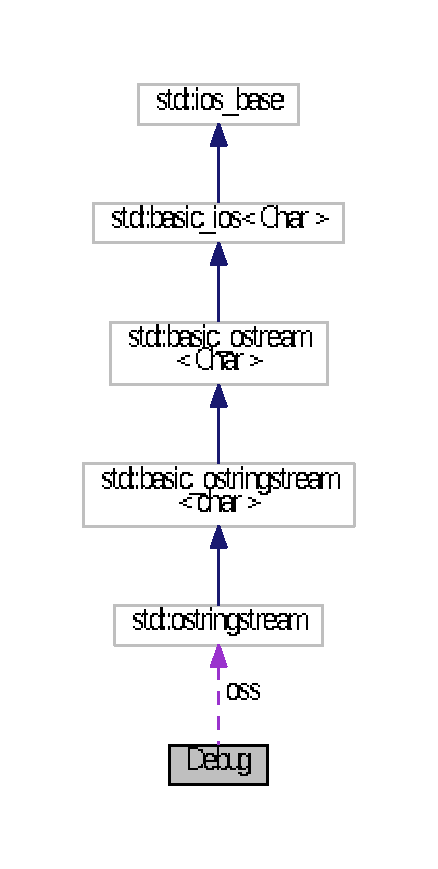
\includegraphics[width=210pt]{classDebug__coll__graph}
\end{center}
\end{figure}
\subsection*{Public Member Functions}
\begin{DoxyCompactItemize}
\item 
\hyperlink{classDebug_a5b453c195c4cfffed2702c3330f53a64}{Debug} ()
\begin{DoxyCompactList}\small\item\em Constructor. \end{DoxyCompactList}\item 
\hyperlink{classDebug_a911a84a0f56b770724e09a049399dc30}{$\sim$\+Debug} ()
\begin{DoxyCompactList}\small\item\em Destructor. \end{DoxyCompactList}\item 
{\footnotesize template$<$typename T $>$ }\\\hyperlink{classDebug}{Debug} \& \hyperlink{classDebug_a7fdf38b9c8d1976b5a723e4bf59fec49}{operator$<$$<$} (const T \&x)
\begin{DoxyCompactList}\small\item\em Stream operator for shoving objects onto a screen somewhere. \end{DoxyCompactList}\item 
\hyperlink{classDebug}{Debug} \& \hyperlink{classDebug_a5e12ec5223bcbbc2f7d6d72c72b37bd7}{operator$<$$<$} (std\+::ostream \&($\ast$pf)(std\+::ostream \&))
\begin{DoxyCompactList}\small\item\em Specialisation for std\+::endl, which is actually a function pointer. \end{DoxyCompactList}\end{DoxyCompactItemize}
\subsection*{Private Attributes}
\begin{DoxyCompactItemize}
\item 
std\+::ostringstream \hyperlink{classDebug_a45f5726114c0078b31b9a0f70199f51e}{oss}
\begin{DoxyCompactList}\small\item\em Stream buffer (avoids theoretical threading issues). \end{DoxyCompactList}\end{DoxyCompactItemize}


\subsection{Detailed Description}
Class for telling the human what playd is doing. 



Definition at line \hyperlink{errors_8hpp_source_l00078}{78} of file \hyperlink{errors_8hpp_source}{errors.\+hpp}.



\subsection{Constructor \& Destructor Documentation}
\hypertarget{classDebug_a5b453c195c4cfffed2702c3330f53a64}{\index{Debug@{Debug}!Debug@{Debug}}
\index{Debug@{Debug}!Debug@{Debug}}
\subsubsection[{Debug}]{\setlength{\rightskip}{0pt plus 5cm}Debug\+::\+Debug (
\begin{DoxyParamCaption}
{}
\end{DoxyParamCaption}
)\hspace{0.3cm}{\ttfamily [inline]}}}\label{classDebug_a5b453c195c4cfffed2702c3330f53a64}


Constructor. 



Definition at line \hyperlink{errors_8hpp_source_l00081}{81} of file \hyperlink{errors_8hpp_source}{errors.\+hpp}.



References \hyperlink{errors_8hpp_source_l00118}{oss}.


\begin{DoxyCode}
00082     \{
00083         \hyperlink{classDebug_a45f5726114c0078b31b9a0f70199f51e}{oss} << \textcolor{stringliteral}{"DEBUG:"};
00084     \}
\end{DoxyCode}
\hypertarget{classDebug_a911a84a0f56b770724e09a049399dc30}{\index{Debug@{Debug}!````~Debug@{$\sim$\+Debug}}
\index{````~Debug@{$\sim$\+Debug}!Debug@{Debug}}
\subsubsection[{$\sim$\+Debug}]{\setlength{\rightskip}{0pt plus 5cm}Debug\+::$\sim$\+Debug (
\begin{DoxyParamCaption}
{}
\end{DoxyParamCaption}
)\hspace{0.3cm}{\ttfamily [inline]}}}\label{classDebug_a911a84a0f56b770724e09a049399dc30}


Destructor. 

Actually shoves things to the screen. 

Definition at line \hyperlink{errors_8hpp_source_l00087}{87} of file \hyperlink{errors_8hpp_source}{errors.\+hpp}.



References \hyperlink{errors_8hpp_source_l00118}{oss}.


\begin{DoxyCode}
00088     \{
00089         std::cerr << \hyperlink{classDebug_a45f5726114c0078b31b9a0f70199f51e}{oss}.str();
00090     \}
\end{DoxyCode}


\subsection{Member Function Documentation}
\hypertarget{classDebug_a7fdf38b9c8d1976b5a723e4bf59fec49}{\index{Debug@{Debug}!operator$<$$<$@{operator$<$$<$}}
\index{operator$<$$<$@{operator$<$$<$}!Debug@{Debug}}
\subsubsection[{operator$<$$<$}]{\setlength{\rightskip}{0pt plus 5cm}template$<$typename T $>$ {\bf Debug}\& Debug\+::operator$<$$<$ (
\begin{DoxyParamCaption}
\item[{const T \&}]{x}
\end{DoxyParamCaption}
)\hspace{0.3cm}{\ttfamily [inline]}}}\label{classDebug_a7fdf38b9c8d1976b5a723e4bf59fec49}


Stream operator for shoving objects onto a screen somewhere. 


\begin{DoxyTemplParams}{Template Parameters}
{\em T} & Type of parameter. \\
\hline
\end{DoxyTemplParams}

\begin{DoxyParams}{Parameters}
{\em x} & Object to write to the stream. \\
\hline
\end{DoxyParams}
\begin{DoxyReturn}{Returns}
Chainable reference. 
\end{DoxyReturn}


Definition at line \hyperlink{errors_8hpp_source_l00099}{99} of file \hyperlink{errors_8hpp_source}{errors.\+hpp}.



References \hyperlink{errors_8hpp_source_l00118}{oss}.


\begin{DoxyCode}
00100     \{
00101         \hyperlink{classDebug_a45f5726114c0078b31b9a0f70199f51e}{oss} << \textcolor{stringliteral}{" "};
00102         \hyperlink{classDebug_a45f5726114c0078b31b9a0f70199f51e}{oss} << x;
00103         \textcolor{keywordflow}{return} *\textcolor{keyword}{this};
00104     \}
\end{DoxyCode}
\hypertarget{classDebug_a5e12ec5223bcbbc2f7d6d72c72b37bd7}{\index{Debug@{Debug}!operator$<$$<$@{operator$<$$<$}}
\index{operator$<$$<$@{operator$<$$<$}!Debug@{Debug}}
\subsubsection[{operator$<$$<$}]{\setlength{\rightskip}{0pt plus 5cm}{\bf Debug}\& Debug\+::operator$<$$<$ (
\begin{DoxyParamCaption}
\item[{std\+::ostream \&($\ast$)(std\+::ostream \&)}]{pf}
\end{DoxyParamCaption}
)\hspace{0.3cm}{\ttfamily [inline]}}}\label{classDebug_a5e12ec5223bcbbc2f7d6d72c72b37bd7}


Specialisation for std\+::endl, which is actually a function pointer. 


\begin{DoxyParams}{Parameters}
{\em pf} & Function pointer. \\
\hline
\end{DoxyParams}
\begin{DoxyReturn}{Returns}
Chainable reference. 
\end{DoxyReturn}


Definition at line \hyperlink{errors_8hpp_source_l00111}{111} of file \hyperlink{errors_8hpp_source}{errors.\+hpp}.



References \hyperlink{errors_8hpp_source_l00118}{oss}.


\begin{DoxyCode}
00112     \{
00113         \hyperlink{classDebug_a45f5726114c0078b31b9a0f70199f51e}{oss} << pf;
00114         \textcolor{keywordflow}{return} *\textcolor{keyword}{this};
00115     \}
\end{DoxyCode}


\subsection{Member Data Documentation}
\hypertarget{classDebug_a45f5726114c0078b31b9a0f70199f51e}{\index{Debug@{Debug}!oss@{oss}}
\index{oss@{oss}!Debug@{Debug}}
\subsubsection[{oss}]{\setlength{\rightskip}{0pt plus 5cm}std\+::ostringstream Debug\+::oss\hspace{0.3cm}{\ttfamily [private]}}}\label{classDebug_a45f5726114c0078b31b9a0f70199f51e}


Stream buffer (avoids theoretical threading issues). 



Definition at line \hyperlink{errors_8hpp_source_l00118}{118} of file \hyperlink{errors_8hpp_source}{errors.\+hpp}.



Referenced by \hyperlink{errors_8hpp_source_l00081}{Debug()}, \hyperlink{errors_8hpp_source_l00099}{operator$<$$<$()}, and \hyperlink{errors_8hpp_source_l00087}{$\sim$\+Debug()}.



The documentation for this class was generated from the following file\+:\begin{DoxyCompactItemize}
\item 
src/\hyperlink{errors_8hpp}{errors.\+hpp}\end{DoxyCompactItemize}

\hypertarget{classError}{\section{Error Class Reference}
\label{classError}\index{Error@{Error}}
}


A playd exception.  




{\ttfamily \#include $<$errors.\+hpp$>$}



Inheritance diagram for Error\+:
\nopagebreak
\begin{figure}[H]
\begin{center}
\leavevmode
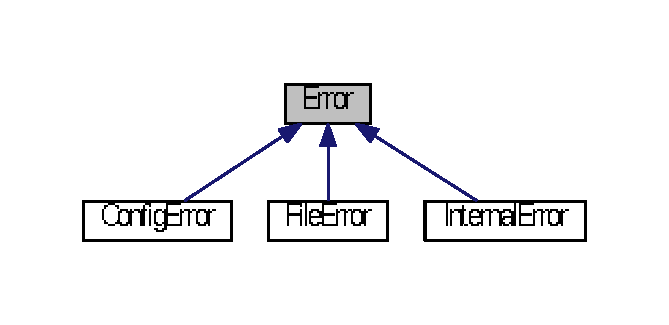
\includegraphics[width=321pt]{classError__inherit__graph}
\end{center}
\end{figure}


Collaboration diagram for Error\+:
\nopagebreak
\begin{figure}[H]
\begin{center}
\leavevmode
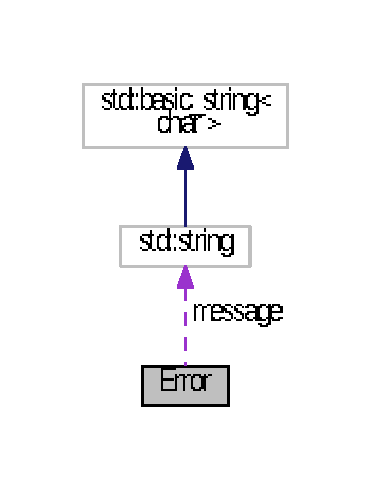
\includegraphics[width=178pt]{classError__coll__graph}
\end{center}
\end{figure}
\subsection*{Public Member Functions}
\begin{DoxyCompactItemize}
\item 
\hyperlink{classError_accd611f3ddae0828adeb6ca251113ffd}{Error} (const std\+::string \&\hyperlink{classError_aa4713ef3ee9c3c0da43a54b01949510d}{message})
\begin{DoxyCompactList}\small\item\em Constructs an \hyperlink{classError}{Error}. \end{DoxyCompactList}\item 
const std\+::string \& \hyperlink{classError_a006605b13a346cf019f60420f1b29b5a}{Message} () const 
\begin{DoxyCompactList}\small\item\em The human-\/readable message for this error. \end{DoxyCompactList}\end{DoxyCompactItemize}
\subsection*{Private Attributes}
\begin{DoxyCompactItemize}
\item 
\hypertarget{classError_aa4713ef3ee9c3c0da43a54b01949510d}{std\+::string \hyperlink{classError_aa4713ef3ee9c3c0da43a54b01949510d}{message}}\label{classError_aa4713ef3ee9c3c0da43a54b01949510d}

\begin{DoxyCompactList}\small\item\em The human-\/readable message for this \hyperlink{classError}{Error}. \end{DoxyCompactList}\end{DoxyCompactItemize}


\subsection{Detailed Description}
A playd exception. 

Definition at line \hyperlink{errors_8hpp_source_l00019}{19} of file \hyperlink{errors_8hpp_source}{errors.\+hpp}.



\subsection{Constructor \& Destructor Documentation}
\hypertarget{classError_accd611f3ddae0828adeb6ca251113ffd}{\index{Error@{Error}!Error@{Error}}
\index{Error@{Error}!Error@{Error}}
\subsubsection[{Error}]{\setlength{\rightskip}{0pt plus 5cm}Error\+::\+Error (
\begin{DoxyParamCaption}
\item[{const std\+::string \&}]{message}
\end{DoxyParamCaption}
)}}\label{classError_accd611f3ddae0828adeb6ca251113ffd}


Constructs an \hyperlink{classError}{Error}. 


\begin{DoxyParams}{Parameters}
{\em message} & The human-\/readable message of the error. \\
\hline
\end{DoxyParams}


Definition at line \hyperlink{errors_8cpp_source_l00012}{12} of file \hyperlink{errors_8cpp_source}{errors.\+cpp}.


\begin{DoxyCode}
00013 \{
00014     this->\hyperlink{classError_aa4713ef3ee9c3c0da43a54b01949510d}{message} = std::string(\hyperlink{classError_aa4713ef3ee9c3c0da43a54b01949510d}{message});
00015 \}
\end{DoxyCode}


\subsection{Member Function Documentation}
\hypertarget{classError_a006605b13a346cf019f60420f1b29b5a}{\index{Error@{Error}!Message@{Message}}
\index{Message@{Message}!Error@{Error}}
\subsubsection[{Message}]{\setlength{\rightskip}{0pt plus 5cm}const std\+::string \& Error\+::\+Message (
\begin{DoxyParamCaption}
{}
\end{DoxyParamCaption}
) const}}\label{classError_a006605b13a346cf019f60420f1b29b5a}


The human-\/readable message for this error. 

\begin{DoxyReturn}{Returns}
A reference to the string describing this \hyperlink{classError}{Error}. 
\end{DoxyReturn}


Definition at line \hyperlink{errors_8cpp_source_l00017}{17} of file \hyperlink{errors_8cpp_source}{errors.\+cpp}.



References \hyperlink{errors_8hpp_source_l00034}{message}.



Referenced by \hyperlink{io__response_8cpp_source_l00033}{Response\+Sink\+::\+Respond\+With\+Error()}.


\begin{DoxyCode}
00018 \{
00019     \textcolor{keywordflow}{return} this->\hyperlink{classError_aa4713ef3ee9c3c0da43a54b01949510d}{message};
00020 \}
\end{DoxyCode}


The documentation for this class was generated from the following files\+:\begin{DoxyCompactItemize}
\item 
src/\hyperlink{errors_8hpp}{errors.\+hpp}\item 
src/\hyperlink{errors_8cpp}{errors.\+cpp}\end{DoxyCompactItemize}

\hypertarget{classFileError}{\section{File\+Error Class Reference}
\label{classFileError}\index{File\+Error@{File\+Error}}
}


An \hyperlink{classError}{Error} signifying that playd can't read a file.  




{\ttfamily \#include $<$errors.\+hpp$>$}



Inheritance diagram for File\+Error\+:
\nopagebreak
\begin{figure}[H]
\begin{center}
\leavevmode
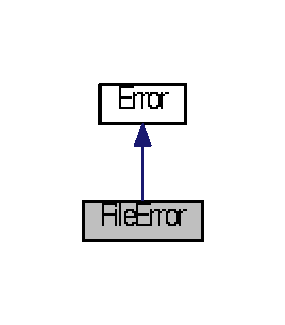
\includegraphics[width=137pt]{classFileError__inherit__graph}
\end{center}
\end{figure}


Collaboration diagram for File\+Error\+:
\nopagebreak
\begin{figure}[H]
\begin{center}
\leavevmode
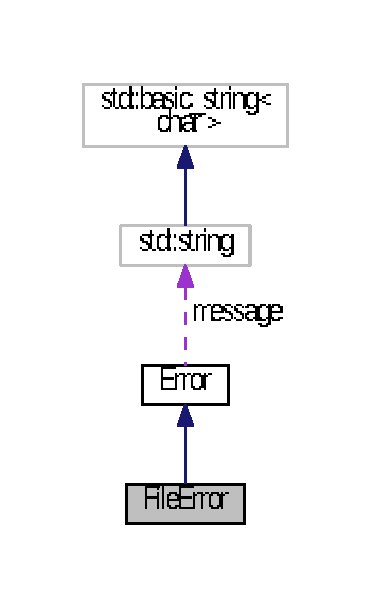
\includegraphics[width=178pt]{classFileError__coll__graph}
\end{center}
\end{figure}
\subsection*{Public Member Functions}
\begin{DoxyCompactItemize}
\item 
\hyperlink{classFileError_a3daf79a4497298aa7d8dbd42897074d2}{File\+Error} (const std\+::string \&\hyperlink{classError_aa4713ef3ee9c3c0da43a54b01949510d}{message})
\begin{DoxyCompactList}\small\item\em Constructs a \hyperlink{classFileError}{File\+Error}. \end{DoxyCompactList}\end{DoxyCompactItemize}


\subsection{Detailed Description}
An \hyperlink{classError}{Error} signifying that playd can't read a file. 

Definition at line \hyperlink{errors_8hpp_source_l00068}{68} of file \hyperlink{errors_8hpp_source}{errors.\+hpp}.



\subsection{Constructor \& Destructor Documentation}
\hypertarget{classFileError_a3daf79a4497298aa7d8dbd42897074d2}{\index{File\+Error@{File\+Error}!File\+Error@{File\+Error}}
\index{File\+Error@{File\+Error}!File\+Error@{File\+Error}}
\subsubsection[{File\+Error}]{\setlength{\rightskip}{0pt plus 5cm}File\+Error\+::\+File\+Error (
\begin{DoxyParamCaption}
\item[{const std\+::string \&}]{message}
\end{DoxyParamCaption}
)\hspace{0.3cm}{\ttfamily [inline]}}}\label{classFileError_a3daf79a4497298aa7d8dbd42897074d2}


Constructs a \hyperlink{classFileError}{File\+Error}. 


\begin{DoxyParams}{Parameters}
{\em message} & The human-\/readable message of the error. \\
\hline
\end{DoxyParams}


Definition at line \hyperlink{errors_8hpp_source_l00074}{74} of file \hyperlink{errors_8hpp_source}{errors.\+hpp}.


\begin{DoxyCode}
00074 : \hyperlink{classError_accd611f3ddae0828adeb6ca251113ffd}{Error}(\hyperlink{classError_aa4713ef3ee9c3c0da43a54b01949510d}{message}) \{\};
\end{DoxyCode}


The documentation for this class was generated from the following file\+:\begin{DoxyCompactItemize}
\item 
src/\hyperlink{errors_8hpp}{errors.\+hpp}\end{DoxyCompactItemize}

\hypertarget{classInternalError}{\section{Internal\+Error Class Reference}
\label{classInternalError}\index{Internal\+Error@{Internal\+Error}}
}


An \hyperlink{classError}{Error} signifying that playd has hit an internal snag.  




{\ttfamily \#include $<$errors.\+hpp$>$}



Inheritance diagram for Internal\+Error\+:
\nopagebreak
\begin{figure}[H]
\begin{center}
\leavevmode
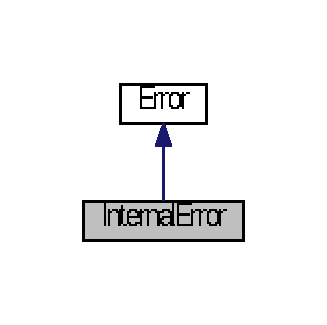
\includegraphics[width=157pt]{classInternalError__inherit__graph}
\end{center}
\end{figure}


Collaboration diagram for Internal\+Error\+:
\nopagebreak
\begin{figure}[H]
\begin{center}
\leavevmode
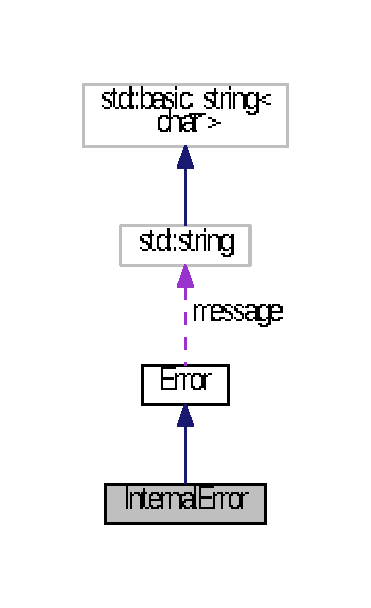
\includegraphics[width=178pt]{classInternalError__coll__graph}
\end{center}
\end{figure}
\subsection*{Public Member Functions}
\begin{DoxyCompactItemize}
\item 
\hyperlink{classInternalError_a02889f0d60c52bb6b92c522c034aa0bf}{Internal\+Error} (const std\+::string \&\hyperlink{classError_aa4713ef3ee9c3c0da43a54b01949510d}{message})
\begin{DoxyCompactList}\small\item\em Constructs an \hyperlink{classInternalError}{Internal\+Error}. \end{DoxyCompactList}\end{DoxyCompactItemize}


\subsection{Detailed Description}
An \hyperlink{classError}{Error} signifying that playd has hit an internal snag. 

Definition at line \hyperlink{errors_8hpp_source_l00056}{56} of file \hyperlink{errors_8hpp_source}{errors.\+hpp}.



\subsection{Constructor \& Destructor Documentation}
\hypertarget{classInternalError_a02889f0d60c52bb6b92c522c034aa0bf}{\index{Internal\+Error@{Internal\+Error}!Internal\+Error@{Internal\+Error}}
\index{Internal\+Error@{Internal\+Error}!Internal\+Error@{Internal\+Error}}
\subsubsection[{Internal\+Error}]{\setlength{\rightskip}{0pt plus 5cm}Internal\+Error\+::\+Internal\+Error (
\begin{DoxyParamCaption}
\item[{const std\+::string \&}]{message}
\end{DoxyParamCaption}
)\hspace{0.3cm}{\ttfamily [inline]}}}\label{classInternalError_a02889f0d60c52bb6b92c522c034aa0bf}


Constructs an \hyperlink{classInternalError}{Internal\+Error}. 


\begin{DoxyParams}{Parameters}
{\em message} & The human-\/readable message of the error. \\
\hline
\end{DoxyParams}


Definition at line \hyperlink{errors_8hpp_source_l00062}{62} of file \hyperlink{errors_8hpp_source}{errors.\+hpp}.


\begin{DoxyCode}
00062 : \hyperlink{classError_accd611f3ddae0828adeb6ca251113ffd}{Error}(\hyperlink{classError_aa4713ef3ee9c3c0da43a54b01949510d}{message}) \{\};
\end{DoxyCode}


The documentation for this class was generated from the following file\+:\begin{DoxyCompactItemize}
\item 
src/\hyperlink{errors_8hpp}{errors.\+hpp}\end{DoxyCompactItemize}

\hypertarget{classIoReactor}{\section{Io\+Reactor Class Reference}
\label{classIoReactor}\index{Io\+Reactor@{Io\+Reactor}}
}


The I\+O reactor, which services input, routes responses, and executes the \hyperlink{classPlayer}{Player} update routine periodically.  




{\ttfamily \#include $<$io\+\_\+reactor.\+hpp$>$}



Inheritance diagram for Io\+Reactor\+:
\nopagebreak
\begin{figure}[H]
\begin{center}
\leavevmode
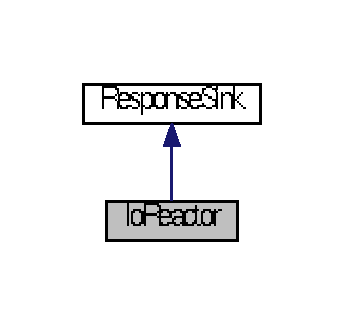
\includegraphics[width=165pt]{classIoReactor__inherit__graph}
\end{center}
\end{figure}


Collaboration diagram for Io\+Reactor\+:
\nopagebreak
\begin{figure}[H]
\begin{center}
\leavevmode
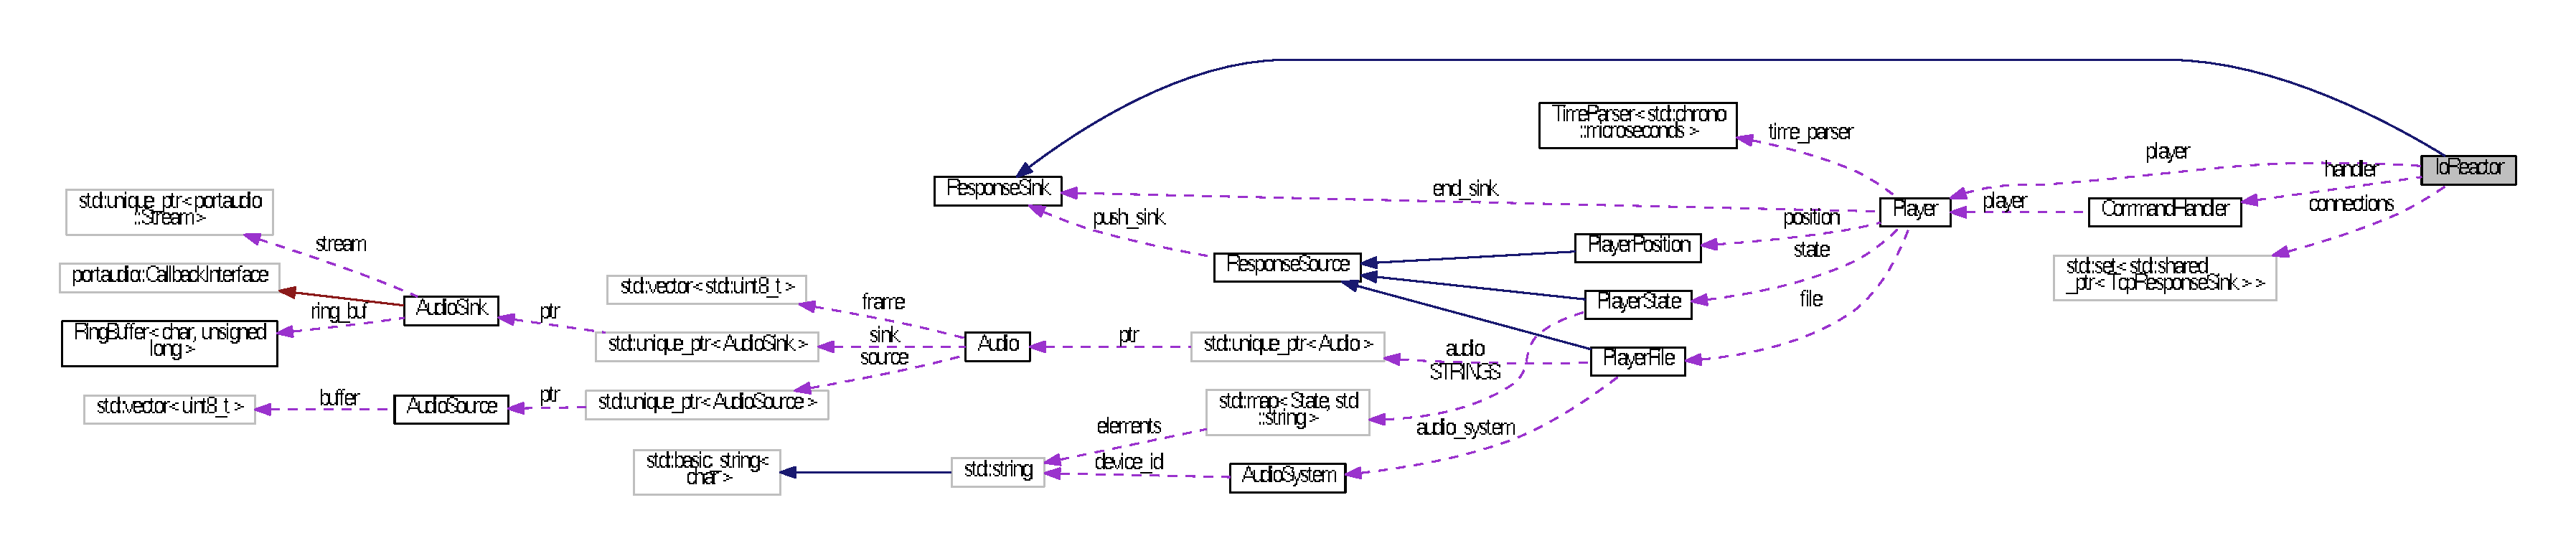
\includegraphics[width=350pt]{classIoReactor__coll__graph}
\end{center}
\end{figure}
\subsection*{Public Member Functions}
\begin{DoxyCompactItemize}
\item 
\hyperlink{classIoReactor_aace954427c447c73caf6b8dbcd367284}{Io\+Reactor} (\hyperlink{classPlayer}{Player} \&\hyperlink{classIoReactor_a795397b36da55b59bff63b455a344dea}{player}, \hyperlink{classCommandHandler}{Command\+Handler} \&\hyperlink{classIoReactor_a81bf838edb7adf1edcb992bfe61d6b78}{handler}, const std\+::string \&address, const std\+::string \&port)
\begin{DoxyCompactList}\small\item\em Constructs an \hyperlink{classIoReactor}{Io\+Reactor}. \end{DoxyCompactList}\item 
\hypertarget{classIoReactor_a5b0292192e98a5e6e0fcd65631b3e0fe}{\hyperlink{classIoReactor_a5b0292192e98a5e6e0fcd65631b3e0fe}{Io\+Reactor} (const \hyperlink{classIoReactor}{Io\+Reactor} \&)=delete}\label{classIoReactor_a5b0292192e98a5e6e0fcd65631b3e0fe}

\begin{DoxyCompactList}\small\item\em Deleted copy constructor. \end{DoxyCompactList}\item 
\hypertarget{classIoReactor_a5e05bcbdf86f3124adb67ce76bf4f8a9}{\hyperlink{classIoReactor}{Io\+Reactor} \& \hyperlink{classIoReactor_a5e05bcbdf86f3124adb67ce76bf4f8a9}{operator=} (const \hyperlink{classIoReactor}{Io\+Reactor} \&)=delete}\label{classIoReactor_a5e05bcbdf86f3124adb67ce76bf4f8a9}

\begin{DoxyCompactList}\small\item\em Deleted copy-\/assignment. \end{DoxyCompactList}\item 
void \hyperlink{classIoReactor_a23f583f9964a6f3f38f983b40f7ae10d}{Run} ()
\begin{DoxyCompactList}\small\item\em Runs the reactor. \end{DoxyCompactList}\item 
void \hyperlink{classIoReactor_a3566c7200adb102579d2c330a2cbf91d}{End} ()
\begin{DoxyCompactList}\small\item\em Ends the reactor. \end{DoxyCompactList}\item 
void \hyperlink{classIoReactor_a535c6ff0899391afc02c87b1dfe7c6e2}{New\+Connection} (uv\+\_\+stream\+\_\+t $\ast$\hyperlink{classIoReactor_a4c9c61af246fda7db1bdd4e2b3170c66}{server})
\begin{DoxyCompactList}\small\item\em Accepts a new connection. \end{DoxyCompactList}\item 
void \hyperlink{classIoReactor_af31bb722acf08d10eaa46ea7a1a5d4ca}{Remove\+Connection} (\hyperlink{classTcpResponseSink}{Tcp\+Response\+Sink} \&sink)
\begin{DoxyCompactList}\small\item\em Removes a connection. \end{DoxyCompactList}\end{DoxyCompactItemize}
\subsection*{Private Member Functions}
\begin{DoxyCompactItemize}
\item 
void \hyperlink{classIoReactor_a4cfe12db93bda3f7b2c29436c4969006}{Respond\+Raw} (const std\+::string \&string) const override
\begin{DoxyCompactList}\small\item\em Outputs a raw response string. \end{DoxyCompactList}\item 
void \hyperlink{classIoReactor_aab8269bf4512c4c74a56998898b3144e}{Init\+Acceptor} (const std\+::string \&address, const std\+::string \&port)
\begin{DoxyCompactList}\small\item\em Initialises a T\+C\+P acceptor on the given address and port. \end{DoxyCompactList}\item 
\hypertarget{classIoReactor_a8a586b8e9545e79db8dc9bca3657388f}{void \hyperlink{classIoReactor_a8a586b8e9545e79db8dc9bca3657388f}{Do\+Update\+Timer} ()}\label{classIoReactor_a8a586b8e9545e79db8dc9bca3657388f}

\begin{DoxyCompactList}\small\item\em Sets up a periodic timer to run the playd update loop. \end{DoxyCompactList}\end{DoxyCompactItemize}
\subsection*{Private Attributes}
\begin{DoxyCompactItemize}
\item 
\hypertarget{classIoReactor_a15617cf44d3c50d5c2d31e8b1812e140}{std\+::set$<$ std\+::shared\+\_\+ptr\\*
$<$ \hyperlink{classTcpResponseSink}{Tcp\+Response\+Sink} $>$ $>$ \hyperlink{classIoReactor_a15617cf44d3c50d5c2d31e8b1812e140}{connections}}\label{classIoReactor_a15617cf44d3c50d5c2d31e8b1812e140}

\begin{DoxyCompactList}\small\item\em The set of connections currently serviced by the \hyperlink{classIoReactor}{Io\+Reactor}. \end{DoxyCompactList}\item 
\hypertarget{classIoReactor_a4c9c61af246fda7db1bdd4e2b3170c66}{uv\+\_\+tcp\+\_\+t \hyperlink{classIoReactor_a4c9c61af246fda7db1bdd4e2b3170c66}{server}}\label{classIoReactor_a4c9c61af246fda7db1bdd4e2b3170c66}

\begin{DoxyCompactList}\small\item\em The libuv handle for the T\+C\+P server. \end{DoxyCompactList}\item 
\hypertarget{classIoReactor_a6364acb721e4a7a1374070e317074bbc}{uv\+\_\+timer\+\_\+t \hyperlink{classIoReactor_a6364acb721e4a7a1374070e317074bbc}{updater}}\label{classIoReactor_a6364acb721e4a7a1374070e317074bbc}

\begin{DoxyCompactList}\small\item\em The libuv handle for the update timer. \end{DoxyCompactList}\item 
\hypertarget{classIoReactor_a795397b36da55b59bff63b455a344dea}{\hyperlink{classPlayer}{Player} \& \hyperlink{classIoReactor_a795397b36da55b59bff63b455a344dea}{player}}\label{classIoReactor_a795397b36da55b59bff63b455a344dea}

\begin{DoxyCompactList}\small\item\em The player. \end{DoxyCompactList}\item 
\hypertarget{classIoReactor_a81bf838edb7adf1edcb992bfe61d6b78}{\hyperlink{classCommandHandler}{Command\+Handler} \& \hyperlink{classIoReactor_a81bf838edb7adf1edcb992bfe61d6b78}{handler}}\label{classIoReactor_a81bf838edb7adf1edcb992bfe61d6b78}

\begin{DoxyCompactList}\small\item\em The command handler. \end{DoxyCompactList}\end{DoxyCompactItemize}
\subsection*{Static Private Attributes}
\begin{DoxyCompactItemize}
\item 
\hypertarget{classIoReactor_a1d8cc56deaa2e801347c21e6490d4f5c}{static const uint16\+\_\+t \hyperlink{classIoReactor_a1d8cc56deaa2e801347c21e6490d4f5c}{P\+L\+A\+Y\+E\+R\+\_\+\+U\+P\+D\+A\+T\+E\+\_\+\+P\+E\+R\+I\+O\+D} = 5}\label{classIoReactor_a1d8cc56deaa2e801347c21e6490d4f5c}

\begin{DoxyCompactList}\small\item\em The period between player updates. \end{DoxyCompactList}\end{DoxyCompactItemize}
\subsection*{Additional Inherited Members}


\subsection{Detailed Description}
The I\+O reactor, which services input, routes responses, and executes the \hyperlink{classPlayer}{Player} update routine periodically. 

Definition at line \hyperlink{io__reactor_8hpp_source_l00035}{35} of file \hyperlink{io__reactor_8hpp_source}{io\+\_\+reactor.\+hpp}.



\subsection{Constructor \& Destructor Documentation}
\hypertarget{classIoReactor_aace954427c447c73caf6b8dbcd367284}{\index{Io\+Reactor@{Io\+Reactor}!Io\+Reactor@{Io\+Reactor}}
\index{Io\+Reactor@{Io\+Reactor}!Io\+Reactor@{Io\+Reactor}}
\subsubsection[{Io\+Reactor}]{\setlength{\rightskip}{0pt plus 5cm}Io\+Reactor\+::\+Io\+Reactor (
\begin{DoxyParamCaption}
\item[{{\bf Player} \&}]{player, }
\item[{{\bf Command\+Handler} \&}]{handler, }
\item[{const std\+::string \&}]{address, }
\item[{const std\+::string \&}]{port}
\end{DoxyParamCaption}
)\hspace{0.3cm}{\ttfamily [explicit]}}}\label{classIoReactor_aace954427c447c73caf6b8dbcd367284}


Constructs an \hyperlink{classIoReactor}{Io\+Reactor}. 


\begin{DoxyParams}{Parameters}
{\em player} & The player to which periodic update requests shall be sent. \\
\hline
{\em handler} & The handler to which command inputs shall be sent. \\
\hline
{\em address} & The address to which \hyperlink{classIoReactor}{Io\+Reactor} will bind. \\
\hline
{\em port} & The port on which \hyperlink{classIoReactor}{Io\+Reactor} will listen for clients. \\
\hline
\end{DoxyParams}


Definition at line \hyperlink{io__reactor_8cpp_source_l00138}{138} of file \hyperlink{io__reactor_8cpp_source}{io\+\_\+reactor.\+cpp}.



References \hyperlink{io__reactor_8cpp_source_l00151}{Do\+Update\+Timer()}, and \hyperlink{io__reactor_8cpp_source_l00159}{Init\+Acceptor()}.


\begin{DoxyCode}
00140     : \hyperlink{classIoReactor_a795397b36da55b59bff63b455a344dea}{player}(player), \hyperlink{classIoReactor_a81bf838edb7adf1edcb992bfe61d6b78}{handler}(handler)
00141 \{
00142     \hyperlink{classIoReactor_aab8269bf4512c4c74a56998898b3144e}{InitAcceptor}(address, port);
00143     \hyperlink{classIoReactor_a8a586b8e9545e79db8dc9bca3657388f}{DoUpdateTimer}();
00144 \}
\end{DoxyCode}


\subsection{Member Function Documentation}
\hypertarget{classIoReactor_a3566c7200adb102579d2c330a2cbf91d}{\index{Io\+Reactor@{Io\+Reactor}!End@{End}}
\index{End@{End}!Io\+Reactor@{Io\+Reactor}}
\subsubsection[{End}]{\setlength{\rightskip}{0pt plus 5cm}void Io\+Reactor\+::\+End (
\begin{DoxyParamCaption}
{}
\end{DoxyParamCaption}
)}}\label{classIoReactor_a3566c7200adb102579d2c330a2cbf91d}


Ends the reactor. 

This should be called by the parent object when the player is quitting. 

Definition at line \hyperlink{io__reactor_8cpp_source_l00183}{183} of file \hyperlink{io__reactor_8cpp_source}{io\+\_\+reactor.\+cpp}.


\begin{DoxyCode}
00184 \{
00185     uv\_stop(uv\_default\_loop());
00186 \}
\end{DoxyCode}
\hypertarget{classIoReactor_aab8269bf4512c4c74a56998898b3144e}{\index{Io\+Reactor@{Io\+Reactor}!Init\+Acceptor@{Init\+Acceptor}}
\index{Init\+Acceptor@{Init\+Acceptor}!Io\+Reactor@{Io\+Reactor}}
\subsubsection[{Init\+Acceptor}]{\setlength{\rightskip}{0pt plus 5cm}void Io\+Reactor\+::\+Init\+Acceptor (
\begin{DoxyParamCaption}
\item[{const std\+::string \&}]{address, }
\item[{const std\+::string \&}]{port}
\end{DoxyParamCaption}
)\hspace{0.3cm}{\ttfamily [private]}}}\label{classIoReactor_aab8269bf4512c4c74a56998898b3144e}


Initialises a T\+C\+P acceptor on the given address and port. 


\begin{DoxyParams}{Parameters}
{\em address} & The I\+Pv4 address on which the T\+C\+P server should listen. \\
\hline
{\em port} & The T\+C\+P port on which the T\+C\+P server should listen. \\
\hline
\end{DoxyParams}


Definition at line \hyperlink{io__reactor_8cpp_source_l00159}{159} of file \hyperlink{io__reactor_8cpp_source}{io\+\_\+reactor.\+cpp}.



References \hyperlink{io__reactor_8hpp_source_l00101}{server}, and \hyperlink{io__reactor_8cpp_source_l00082}{Uv\+Listen\+Callback()}.



Referenced by \hyperlink{io__reactor_8cpp_source_l00138}{Io\+Reactor()}.


\begin{DoxyCode}
00161 \{
00162     \textcolor{keywordtype}{int} uport = std::stoi(port);
00163 
00164     uv\_tcp\_init(uv\_default\_loop(), &this->\hyperlink{classIoReactor_a4c9c61af246fda7db1bdd4e2b3170c66}{server});
00165     this->\hyperlink{classIoReactor_a4c9c61af246fda7db1bdd4e2b3170c66}{server}.data = \textcolor{keyword}{static\_cast<}\textcolor{keywordtype}{void} *\textcolor{keyword}{>}(\textcolor{keyword}{this});
00166 
00167     \textcolor{keyword}{struct }sockaddr\_in bind\_addr;
00168     uv\_ip4\_addr(address.c\_str(), uport, &bind\_addr);
00169     uv\_tcp\_bind(&this->\hyperlink{classIoReactor_a4c9c61af246fda7db1bdd4e2b3170c66}{server}, (\textcolor{keyword}{const} sockaddr *)&bind\_addr, 0);
00170 
00171     \textcolor{comment}{// TODO: Handle errors from uv\_listen.}
00172     uv\_listen((uv\_stream\_t *)&this->\hyperlink{classIoReactor_a4c9c61af246fda7db1bdd4e2b3170c66}{server}, 128, \hyperlink{io__reactor_8cpp_ab1a411534cf6420d24748b0e78927ebf}{UvListenCallback});
00173     \hyperlink{classDebug}{Debug}() << \textcolor{stringliteral}{"Listening at"} << address << \textcolor{stringliteral}{"on"} << port << std::endl;
00174 \}
\end{DoxyCode}
\hypertarget{classIoReactor_a535c6ff0899391afc02c87b1dfe7c6e2}{\index{Io\+Reactor@{Io\+Reactor}!New\+Connection@{New\+Connection}}
\index{New\+Connection@{New\+Connection}!Io\+Reactor@{Io\+Reactor}}
\subsubsection[{New\+Connection}]{\setlength{\rightskip}{0pt plus 5cm}void Io\+Reactor\+::\+New\+Connection (
\begin{DoxyParamCaption}
\item[{uv\+\_\+stream\+\_\+t $\ast$}]{server}
\end{DoxyParamCaption}
)}}\label{classIoReactor_a535c6ff0899391afc02c87b1dfe7c6e2}


Accepts a new connection. 

This accepts the connection, and adds it to this \hyperlink{classIoReactor}{Io\+Reactor}'s connection pool.

This should be called with a server that has just received a new connection.


\begin{DoxyParams}{Parameters}
{\em server} & Pointer to the libuv server accepting connections.\\
\hline
\end{DoxyParams}
\begin{DoxyRefDesc}{Todo}
\item[\hyperlink{todo__todo000004}{Todo}]This isn't a great fit for the public interface of \hyperlink{classIoReactor}{Io\+Reactor} -\/ separate into a Connection\+Pool class? \end{DoxyRefDesc}


Definition at line \hyperlink{io__reactor_8cpp_source_l00114}{114} of file \hyperlink{io__reactor_8cpp_source}{io\+\_\+reactor.\+cpp}.



References \hyperlink{io__reactor_8hpp_source_l00096}{connections}, \hyperlink{io__reactor_8hpp_source_l00105}{handler}, \hyperlink{io__reactor_8hpp_source_l00104}{player}, \hyperlink{io__reactor_8cpp_source_l00058}{Uv\+Alloc()}, \hyperlink{io__reactor_8cpp_source_l00064}{Uv\+Close\+Callback()}, \hyperlink{io__reactor_8cpp_source_l00075}{Uv\+Read\+Callback()}, and \hyperlink{player_8cpp_source_l00058}{Player\+::\+Welcome\+Client()}.



Referenced by \hyperlink{io__reactor_8cpp_source_l00082}{Uv\+Listen\+Callback()}.


\begin{DoxyCode}
00115 \{
00116     uv\_tcp\_t *client = \textcolor{keyword}{new} uv\_tcp\_t();
00117     uv\_tcp\_init(uv\_default\_loop(), client);
00118 
00119     \textcolor{keywordflow}{if} (uv\_accept(\hyperlink{classIoReactor_a4c9c61af246fda7db1bdd4e2b3170c66}{server}, (uv\_stream\_t *)client) == 0) \{
00120         \hyperlink{classDebug}{Debug}() << \textcolor{stringliteral}{"New connection"} << std::endl;
00121         \textcolor{keyword}{auto} tcp = std::make\_shared<TcpResponseSink>(*\textcolor{keyword}{this}, client,
00122                                                      this->\hyperlink{classIoReactor_a81bf838edb7adf1edcb992bfe61d6b78}{handler});
00123         this->\hyperlink{classIoReactor_a795397b36da55b59bff63b455a344dea}{player}.\hyperlink{classPlayer_aac35c9a49758150d5c5e0ea2fcd94d16}{WelcomeClient}(*tcp);
00124         this->\hyperlink{classIoReactor_a15617cf44d3c50d5c2d31e8b1812e140}{connections}.insert(tcp);
00125         client->data = \textcolor{keyword}{static\_cast<}\textcolor{keywordtype}{void} *\textcolor{keyword}{>}(tcp.get());
00126 
00127         uv\_read\_start((uv\_stream\_t *)client, \hyperlink{io__reactor_8cpp_ab0c51a1d8447db72e81a13d45448b85f}{UvAlloc}, \hyperlink{io__reactor_8cpp_a8c1937e7aebd228e6a5eab19f1add9f9}{UvReadCallback});
00128     \} \textcolor{keywordflow}{else} \{
00129         uv\_close((uv\_handle\_t *)client, \hyperlink{io__reactor_8cpp_ab85791c3e9c737453047decfbb7388f4}{UvCloseCallback});
00130     \}
00131 \}
\end{DoxyCode}
\hypertarget{classIoReactor_af31bb722acf08d10eaa46ea7a1a5d4ca}{\index{Io\+Reactor@{Io\+Reactor}!Remove\+Connection@{Remove\+Connection}}
\index{Remove\+Connection@{Remove\+Connection}!Io\+Reactor@{Io\+Reactor}}
\subsubsection[{Remove\+Connection}]{\setlength{\rightskip}{0pt plus 5cm}void Io\+Reactor\+::\+Remove\+Connection (
\begin{DoxyParamCaption}
\item[{{\bf Tcp\+Response\+Sink} \&}]{sink}
\end{DoxyParamCaption}
)}}\label{classIoReactor_af31bb722acf08d10eaa46ea7a1a5d4ca}


Removes a connection. 


\begin{DoxyParams}{Parameters}
{\em sink} & The connection to remove.\\
\hline
\end{DoxyParams}
\begin{DoxyRefDesc}{Todo}
\item[\hyperlink{todo__todo000005}{Todo}]Rename sink? 

This isn't a great fit for the public interface of \hyperlink{classIoReactor}{Io\+Reactor} -\/ separate into a Connection\+Pool class? \end{DoxyRefDesc}


Definition at line \hyperlink{io__reactor_8cpp_source_l00133}{133} of file \hyperlink{io__reactor_8cpp_source}{io\+\_\+reactor.\+cpp}.



References \hyperlink{io__reactor_8hpp_source_l00096}{connections}.



Referenced by \hyperlink{io__reactor_8cpp_source_l00230}{Tcp\+Response\+Sink\+::\+Close()}.


\begin{DoxyCode}
00134 \{
00135     this->\hyperlink{classIoReactor_a15617cf44d3c50d5c2d31e8b1812e140}{connections}.erase(std::make\_shared<TcpResponseSink>(conn));
00136 \}
\end{DoxyCode}
\hypertarget{classIoReactor_a4cfe12db93bda3f7b2c29436c4969006}{\index{Io\+Reactor@{Io\+Reactor}!Respond\+Raw@{Respond\+Raw}}
\index{Respond\+Raw@{Respond\+Raw}!Io\+Reactor@{Io\+Reactor}}
\subsubsection[{Respond\+Raw}]{\setlength{\rightskip}{0pt plus 5cm}void Io\+Reactor\+::\+Respond\+Raw (
\begin{DoxyParamCaption}
\item[{const std\+::string \&}]{string}
\end{DoxyParamCaption}
) const\hspace{0.3cm}{\ttfamily [override]}, {\ttfamily [private]}, {\ttfamily [virtual]}}}\label{classIoReactor_a4cfe12db93bda3f7b2c29436c4969006}


Outputs a raw response string. 


\begin{DoxyParams}{Parameters}
{\em string} & The response string, of the form \char`\"{}\+C\+O\+D\+E message\char`\"{}. \\
\hline
\end{DoxyParams}


Implements \hyperlink{classResponseSink_a128a514e39f23f2bcc97fea62e9de3c5}{Response\+Sink}.



Definition at line \hyperlink{io__reactor_8cpp_source_l00176}{176} of file \hyperlink{io__reactor_8cpp_source}{io\+\_\+reactor.\+cpp}.



References \hyperlink{io__reactor_8hpp_source_l00096}{connections}.


\begin{DoxyCode}
00177 \{
00178     \textcolor{keywordflow}{for} (\textcolor{keyword}{const} \textcolor{keyword}{auto} &conn : this->\hyperlink{classIoReactor_a15617cf44d3c50d5c2d31e8b1812e140}{connections}) \{
00179         conn->RespondRaw(\textcolor{keywordtype}{string});
00180     \}
00181 \}
\end{DoxyCode}
\hypertarget{classIoReactor_a23f583f9964a6f3f38f983b40f7ae10d}{\index{Io\+Reactor@{Io\+Reactor}!Run@{Run}}
\index{Run@{Run}!Io\+Reactor@{Io\+Reactor}}
\subsubsection[{Run}]{\setlength{\rightskip}{0pt plus 5cm}void Io\+Reactor\+::\+Run (
\begin{DoxyParamCaption}
{}
\end{DoxyParamCaption}
)}}\label{classIoReactor_a23f583f9964a6f3f38f983b40f7ae10d}


Runs the reactor. 

It will block until terminated. 

Definition at line \hyperlink{io__reactor_8cpp_source_l00146}{146} of file \hyperlink{io__reactor_8cpp_source}{io\+\_\+reactor.\+cpp}.


\begin{DoxyCode}
00147 \{
00148     uv\_run(uv\_default\_loop(), UV\_RUN\_DEFAULT);
00149 \}
\end{DoxyCode}


The documentation for this class was generated from the following files\+:\begin{DoxyCompactItemize}
\item 
src/io/\hyperlink{io__reactor_8hpp}{io\+\_\+reactor.\+hpp}\item 
src/io/\hyperlink{io__reactor_8cpp}{io\+\_\+reactor.\+cpp}\end{DoxyCompactItemize}

\hypertarget{classplayd}{\section{playd Class Reference}
\label{classplayd}\index{playd@{playd}}
}


The playd application.  




{\ttfamily \#include $<$main.\+hpp$>$}



Collaboration diagram for playd\+:
\nopagebreak
\begin{figure}[H]
\begin{center}
\leavevmode
\includegraphics[width=350pt]{classplayd__coll__graph}
\end{center}
\end{figure}
\subsection*{Public Member Functions}
\begin{DoxyCompactItemize}
\item 
\hyperlink{classplayd_a2dfa519ee11ce75fbe389fcf3b15e122}{playd} (int argc, char $\ast$argv\mbox{[}$\,$\mbox{]})
\begin{DoxyCompactList}\small\item\em Constructs a playd, initialising its libraries. \end{DoxyCompactList}\item 
int \hyperlink{classplayd_aee84626965c812db03120ebe3267fcab}{Run} ()
\begin{DoxyCompactList}\small\item\em Runs playd. \end{DoxyCompactList}\end{DoxyCompactItemize}
\subsection*{Private Member Functions}
\begin{DoxyCompactItemize}
\item 
int \hyperlink{classplayd_a767d029a5d1321e912c1a2a92e8f3c64}{Get\+Device\+I\+D} ()
\begin{DoxyCompactList}\small\item\em Tries to get the output device I\+D from program arguments. \end{DoxyCompactList}\item 
void \hyperlink{classplayd_a9b32921db2f987d1faa28cbac50a0ed3}{List\+Output\+Devices} ()
\begin{DoxyCompactList}\small\item\em Lists on stdout all sound devices to which the audio output may connect. \end{DoxyCompactList}\item 
void \hyperlink{classplayd_a9fa7e8f2ccbd46c10bd604bb510d6304}{Register\+Commands} (\hyperlink{classPlayer}{Player} $\ast$p)
\begin{DoxyCompactList}\small\item\em Registers the playd command set on the given \hyperlink{classPlayer}{Player}. \end{DoxyCompactList}\end{DoxyCompactItemize}
\subsection*{Private Attributes}
\begin{DoxyCompactItemize}
\item 
\hypertarget{classplayd_a58d45d86bd51dea16f476aae648ff63c}{std\+::vector$<$ std\+::string $>$ \hyperlink{classplayd_a58d45d86bd51dea16f476aae648ff63c}{arguments}}\label{classplayd_a58d45d86bd51dea16f476aae648ff63c}

\begin{DoxyCompactList}\small\item\em The argument vector. \end{DoxyCompactList}\item 
\hypertarget{classplayd_a2c7193680bd18f1e9b3f63f2234485de}{\hyperlink{classAudioSystem}{Audio\+System} \hyperlink{classplayd_a2c7193680bd18f1e9b3f63f2234485de}{audio}}\label{classplayd_a2c7193680bd18f1e9b3f63f2234485de}

\begin{DoxyCompactList}\small\item\em The audio subsystem. \end{DoxyCompactList}\item 
\hypertarget{classplayd_a8712fc23f3139a2fd2e9dbfb24b998dd}{\hyperlink{classPlayer}{Player} \hyperlink{classplayd_a8712fc23f3139a2fd2e9dbfb24b998dd}{player}}\label{classplayd_a8712fc23f3139a2fd2e9dbfb24b998dd}

\begin{DoxyCompactList}\small\item\em The player subsystem. \end{DoxyCompactList}\item 
\hypertarget{classplayd_a738bb18c13d3fd7db82ce000dd43d604}{\hyperlink{classCommandHandler}{Command\+Handler} \hyperlink{classplayd_a738bb18c13d3fd7db82ce000dd43d604}{handler}}\label{classplayd_a738bb18c13d3fd7db82ce000dd43d604}

\begin{DoxyCompactList}\small\item\em The command handler. \end{DoxyCompactList}\item 
\hypertarget{classplayd_af9e02b98b1eadecaab2941481dfb803b}{\hyperlink{classPlayer_ab2c65f4a7cbaf6aab6fafbb5633a42c4}{Player\+::\+T\+P} \hyperlink{classplayd_af9e02b98b1eadecaab2941481dfb803b}{time\+\_\+parser}}\label{classplayd_af9e02b98b1eadecaab2941481dfb803b}

\begin{DoxyCompactList}\small\item\em The seek time parser. \end{DoxyCompactList}\item 
\hypertarget{classplayd_a066cb450455e1359e4f80cfa5ecb5c05}{std\+::unique\+\_\+ptr$<$ \hyperlink{classIoReactor}{Io\+Reactor} $>$ \hyperlink{classplayd_a066cb450455e1359e4f80cfa5ecb5c05}{io}}\label{classplayd_a066cb450455e1359e4f80cfa5ecb5c05}

\begin{DoxyCompactList}\small\item\em The I/\+O handler. \end{DoxyCompactList}\end{DoxyCompactItemize}
\subsection*{Static Private Attributes}
\begin{DoxyCompactItemize}
\item 
\hypertarget{classplayd_a540bcb2dac9488bcb8e593378005bd07}{static const \\*
std\+::chrono\+::microseconds \hyperlink{classplayd_a540bcb2dac9488bcb8e593378005bd07}{P\+O\+S\+I\+T\+I\+O\+N\+\_\+\+P\+E\+R\+I\+O\+D}}\label{classplayd_a540bcb2dac9488bcb8e593378005bd07}

\begin{DoxyCompactList}\small\item\em The period between position announcements from the \hyperlink{classPlayer}{Player} object. \end{DoxyCompactList}\end{DoxyCompactItemize}


\subsection{Detailed Description}
The playd application. 

This class contains all the state required by playd, with the exception of that introduced by external C libraries. It is a R\+A\+I\+I class, so constructing playd will load playd's library dependencies, and destructing it will unload them. It is probably not safe to create more than one playd. 

Definition at line \hyperlink{main_8hpp_source_l00029}{29} of file \hyperlink{main_8hpp_source}{main.\+hpp}.



\subsection{Constructor \& Destructor Documentation}
\hypertarget{classplayd_a2dfa519ee11ce75fbe389fcf3b15e122}{\index{playd@{playd}!playd@{playd}}
\index{playd@{playd}!playd@{playd}}
\subsubsection[{playd}]{\setlength{\rightskip}{0pt plus 5cm}playd\+::playd (
\begin{DoxyParamCaption}
\item[{int}]{argc, }
\item[{char $\ast$}]{argv\mbox{[}$\,$\mbox{]}}
\end{DoxyParamCaption}
)}}\label{classplayd_a2dfa519ee11ce75fbe389fcf3b15e122}


Constructs a playd, initialising its libraries. 


\begin{DoxyParams}{Parameters}
{\em argc} & The argument count from the main function. \\
\hline
{\em argv} & The argument vector from the main function. \\
\hline
\end{DoxyParams}


Definition at line \hyperlink{main_8cpp_source_l00115}{115} of file \hyperlink{main_8cpp_source}{main.\+cpp}.



References \hyperlink{main_8hpp_source_l00048}{arguments}, \hyperlink{main_8hpp_source_l00051}{handler}, \hyperlink{main_8hpp_source_l00053}{io}, and \hyperlink{main_8hpp_source_l00050}{player}.


\begin{DoxyCode}
00116     : \hyperlink{classplayd_a2c7193680bd18f1e9b3f63f2234485de}{audio}(), \hyperlink{classplayd_a8712fc23f3139a2fd2e9dbfb24b998dd}{player}(\hyperlink{classplayd_a2c7193680bd18f1e9b3f63f2234485de}{audio}, \hyperlink{classplayd_af9e02b98b1eadecaab2941481dfb803b}{time\_parser}), \hyperlink{classplayd_a738bb18c13d3fd7db82ce000dd43d604}{handler}(
      \hyperlink{classplayd_a8712fc23f3139a2fd2e9dbfb24b998dd}{player}), \hyperlink{classplayd_af9e02b98b1eadecaab2941481dfb803b}{time\_parser}(\hyperlink{main_8cpp_a889c521ce751c2db7ba216a612c1d784}{UNITS})
00117 \{
00118     \textcolor{keywordflow}{for} (\textcolor{keywordtype}{int} i = 0; i < argc; i++) \{
00119         this->\hyperlink{classplayd_a58d45d86bd51dea16f476aae648ff63c}{arguments}.push\_back(std::string(argv[i]));
00120     \}
00121 
00122     \textcolor{keyword}{auto} size = this->\hyperlink{classplayd_a58d45d86bd51dea16f476aae648ff63c}{arguments}.size();
00123 
00124     std::string addr = size > 2 ? this->\hyperlink{classplayd_a58d45d86bd51dea16f476aae648ff63c}{arguments}.at(2) : \textcolor{stringliteral}{"0.0.0.0"};
00125     std::string port = size > 3 ? this->\hyperlink{classplayd_a58d45d86bd51dea16f476aae648ff63c}{arguments}.at(3) : \textcolor{stringliteral}{"1350"};
00126     this->\hyperlink{classplayd_a066cb450455e1359e4f80cfa5ecb5c05}{io} = decltype(this->\hyperlink{classplayd_a066cb450455e1359e4f80cfa5ecb5c05}{io})(
00127                     \textcolor{keyword}{new} \hyperlink{classIoReactor}{IoReactor}(this->\hyperlink{classplayd_a8712fc23f3139a2fd2e9dbfb24b998dd}{player}, this->\hyperlink{classplayd_a738bb18c13d3fd7db82ce000dd43d604}{handler}, addr, port));
00128 \}
\end{DoxyCode}


\subsection{Member Function Documentation}
\hypertarget{classplayd_a767d029a5d1321e912c1a2a92e8f3c64}{\index{playd@{playd}!Get\+Device\+I\+D@{Get\+Device\+I\+D}}
\index{Get\+Device\+I\+D@{Get\+Device\+I\+D}!playd@{playd}}
\subsubsection[{Get\+Device\+I\+D}]{\setlength{\rightskip}{0pt plus 5cm}int playd\+::\+Get\+Device\+I\+D (
\begin{DoxyParamCaption}
{}
\end{DoxyParamCaption}
)\hspace{0.3cm}{\ttfamily [private]}}}\label{classplayd_a767d029a5d1321e912c1a2a92e8f3c64}


Tries to get the output device I\+D from program arguments. 

\begin{DoxyReturn}{Returns}
The device I\+D, -\/1 if invalid selection (or none). 
\end{DoxyReturn}


Definition at line \hyperlink{main_8cpp_source_l00040}{40} of file \hyperlink{main_8cpp_source}{main.\+cpp}.



References \hyperlink{main_8hpp_source_l00048}{arguments}, \hyperlink{main_8hpp_source_l00049}{audio}, \hyperlink{audio__system_8cpp_source_l00055}{Audio\+System\+::\+Get\+Devices\+Info()}, and \hyperlink{audio__system_8cpp_source_l00069}{Audio\+System\+::\+Is\+Output\+Device()}.



Referenced by \hyperlink{main_8cpp_source_l00130}{Run()}.


\begin{DoxyCode}
00041 \{
00042     \textcolor{keywordflow}{if} (this->\hyperlink{classplayd_a58d45d86bd51dea16f476aae648ff63c}{arguments}.size() < 2) \textcolor{keywordflow}{return} -1;
00043 
00044     \textcolor{comment}{/* Only accept valid numbers. */}
00045     \textcolor{keywordtype}{int} id;
00046     \textcolor{keywordflow}{try}
00047     \{
00048         \textcolor{keywordtype}{id} = std::stoi(this->\hyperlink{classplayd_a58d45d86bd51dea16f476aae648ff63c}{arguments}[1]);
00049     \}
00050     \textcolor{keywordflow}{catch} (...)
00051     \{
00052         \textcolor{comment}{/* Only std::invalid\_argument and std::out\_of\_range are thrown}
00053 \textcolor{comment}{         * here. */}
00054         \textcolor{keywordflow}{return} -1;
00055     \}
00056 
00057     \textcolor{comment}{/* Only allow valid (output) devices. */}
00058     \textcolor{keyword}{auto} device\_list = this->\hyperlink{classplayd_a2c7193680bd18f1e9b3f63f2234485de}{audio}.\hyperlink{classAudioSystem_aa268faeb9243c18588631024958856e6}{GetDevicesInfo}();
00059     \textcolor{keywordflow}{if} (this->\hyperlink{classplayd_a2c7193680bd18f1e9b3f63f2234485de}{audio}.\hyperlink{classAudioSystem_a001cd82f854883b80b3ed7d35795581b}{IsOutputDevice}(\textcolor{keywordtype}{id})) \{
00060         \textcolor{keywordflow}{return} id;
00061     \}
00062 
00063     \textcolor{keywordflow}{return} -1;
00064 \}
\end{DoxyCode}
\hypertarget{classplayd_a9b32921db2f987d1faa28cbac50a0ed3}{\index{playd@{playd}!List\+Output\+Devices@{List\+Output\+Devices}}
\index{List\+Output\+Devices@{List\+Output\+Devices}!playd@{playd}}
\subsubsection[{List\+Output\+Devices}]{\setlength{\rightskip}{0pt plus 5cm}void playd\+::\+List\+Output\+Devices (
\begin{DoxyParamCaption}
{}
\end{DoxyParamCaption}
)\hspace{0.3cm}{\ttfamily [private]}}}\label{classplayd_a9b32921db2f987d1faa28cbac50a0ed3}


Lists on stdout all sound devices to which the audio output may connect. 

This is mainly for the benefit of the end user. \hypertarget{classplayd_a9fa7e8f2ccbd46c10bd604bb510d6304}{\index{playd@{playd}!Register\+Commands@{Register\+Commands}}
\index{Register\+Commands@{Register\+Commands}!playd@{playd}}
\subsubsection[{Register\+Commands}]{\setlength{\rightskip}{0pt plus 5cm}void playd\+::\+Register\+Commands (
\begin{DoxyParamCaption}
\item[{{\bf Player} $\ast$}]{p}
\end{DoxyParamCaption}
)\hspace{0.3cm}{\ttfamily [private]}}}\label{classplayd_a9fa7e8f2ccbd46c10bd604bb510d6304}


Registers the playd command set on the given \hyperlink{classPlayer}{Player}. 


\begin{DoxyParams}{Parameters}
{\em p} & The \hyperlink{classPlayer}{Player} on which the commands will act. \\
\hline
\end{DoxyParams}
\hypertarget{classplayd_aee84626965c812db03120ebe3267fcab}{\index{playd@{playd}!Run@{Run}}
\index{Run@{Run}!playd@{playd}}
\subsubsection[{Run}]{\setlength{\rightskip}{0pt plus 5cm}int playd\+::\+Run (
\begin{DoxyParamCaption}
{}
\end{DoxyParamCaption}
)}}\label{classplayd_aee84626965c812db03120ebe3267fcab}


Runs playd. 

\begin{DoxyReturn}{Returns}
The exit code, which may be returned by the program. 
\end{DoxyReturn}


Definition at line \hyperlink{main_8cpp_source_l00130}{130} of file \hyperlink{main_8cpp_source}{main.\+cpp}.



References \hyperlink{main_8hpp_source_l00049}{audio}, \hyperlink{main_8cpp_source_l00040}{Get\+Device\+I\+D()}, \hyperlink{audio__system_8cpp_source_l00055}{Audio\+System\+::\+Get\+Devices\+Info()}, \hyperlink{main_8hpp_source_l00053}{io}, \hyperlink{main_8hpp_source_l00050}{player}, \hyperlink{main_8hpp_source_l00046}{P\+O\+S\+I\+T\+I\+O\+N\+\_\+\+P\+E\+R\+I\+O\+D}, \hyperlink{audio__system_8cpp_source_l00078}{Audio\+System\+::\+Set\+Device\+I\+D()}, \hyperlink{player__position_8cpp_source_l00021}{Player\+::\+Set\+Position\+Response\+Period()}, and \hyperlink{player_8cpp_source_l00067}{Player\+::\+Set\+Response\+Sink()}.



Referenced by \hyperlink{main_8cpp_source_l00028}{main()}.


\begin{DoxyCode}
00131 \{
00132     \textcolor{keywordflow}{try}
00133     \{
00134         \textcolor{comment}{// Don't roll this into the constructor: it'll go out of scope!}
00135         \textcolor{keywordtype}{int} \textcolor{keywordtype}{id} = this->\hyperlink{classplayd_a767d029a5d1321e912c1a2a92e8f3c64}{GetDeviceID}();
00136         \textcolor{keywordflow}{if} (\textcolor{keywordtype}{id} == -1) \{
00137             \textcolor{comment}{/* Oops, user entered an invalid sound device. */}
00138             \textcolor{keyword}{auto} device\_list = this->\hyperlink{classplayd_a2c7193680bd18f1e9b3f63f2234485de}{audio}.\hyperlink{classAudioSystem_aa268faeb9243c18588631024958856e6}{GetDevicesInfo}();
00139             \textcolor{keywordflow}{for} (\textcolor{keyword}{const} \textcolor{keyword}{auto} &device : device\_list) \{
00140                 std::cout << device.first << \textcolor{stringliteral}{": "}
00141                           << device.second << std::endl;
00142             \}
00143             \textcolor{keywordflow}{return} EXIT\_FAILURE;
00144         \}
00145         this->\hyperlink{classplayd_a2c7193680bd18f1e9b3f63f2234485de}{audio}.\hyperlink{classAudioSystem_ade3b400828991d02e36a0b61302d30d2}{SetDeviceID}(\textcolor{keywordtype}{id});
00146 
00147         this->\hyperlink{classplayd_a8712fc23f3139a2fd2e9dbfb24b998dd}{player}.\hyperlink{classPlayer_a1e65e04dae199230d80639112ac07288}{SetPositionResponsePeriod}(
      \hyperlink{classplayd_a540bcb2dac9488bcb8e593378005bd07}{POSITION\_PERIOD});
00148         this->\hyperlink{classplayd_a8712fc23f3139a2fd2e9dbfb24b998dd}{player}.\hyperlink{classPlayer_a719de5af4d1534c2d805a19d5d995deb}{SetResponseSink}(*this->\hyperlink{classplayd_a066cb450455e1359e4f80cfa5ecb5c05}{io});
00149         this->\hyperlink{classplayd_a066cb450455e1359e4f80cfa5ecb5c05}{io}->Run();
00150     \}
00151     \textcolor{keywordflow}{catch} (\hyperlink{classError}{Error} &error)
00152     \{
00153         \hyperlink{classplayd_a066cb450455e1359e4f80cfa5ecb5c05}{io}->RespondWithError(error);
00154         \hyperlink{classDebug}{Debug}() << \textcolor{stringliteral}{"Unhandled exception caught, going away now."}
00155                 << std::endl;
00156         \textcolor{keywordflow}{return} EXIT\_FAILURE;
00157     \}
00158 
00159     \textcolor{keywordflow}{return} EXIT\_SUCCESS;
00160 \}
\end{DoxyCode}


The documentation for this class was generated from the following files\+:\begin{DoxyCompactItemize}
\item 
src/\hyperlink{main_8hpp}{main.\+hpp}\item 
src/\hyperlink{main_8cpp}{main.\+cpp}\end{DoxyCompactItemize}

\hypertarget{classPlayer}{\section{Player Class Reference}
\label{classPlayer}\index{Player@{Player}}
}


A \hyperlink{classPlayer}{Player} contains a loaded audio file and the state of its playback.  




{\ttfamily \#include $<$player.\+hpp$>$}



Collaboration diagram for Player\+:
\nopagebreak
\begin{figure}[H]
\begin{center}
\leavevmode
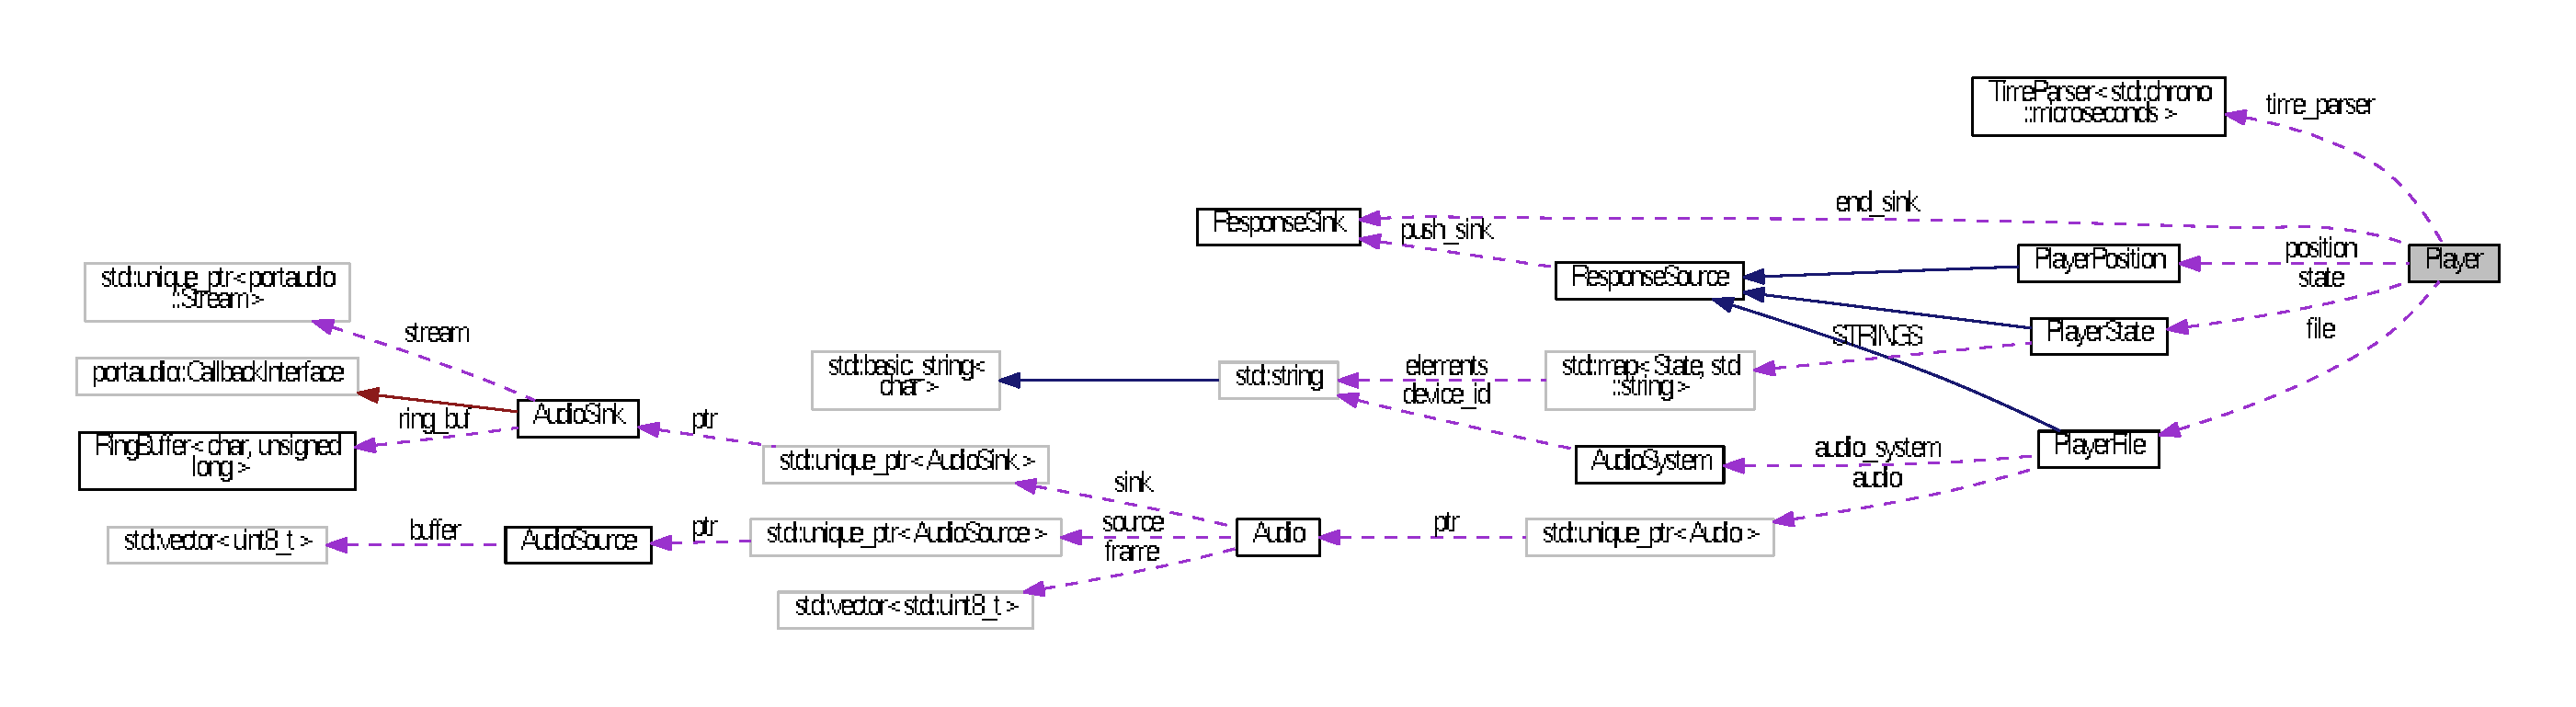
\includegraphics[width=350pt]{classPlayer__coll__graph}
\end{center}
\end{figure}
\subsection*{Public Types}
\begin{DoxyCompactItemize}
\item 
\hypertarget{classPlayer_ab2c65f4a7cbaf6aab6fafbb5633a42c4}{using \hyperlink{classPlayer_ab2c65f4a7cbaf6aab6fafbb5633a42c4}{T\+P} = \hyperlink{classTimeParser}{Time\+Parser}$<$ std\+::chrono\+::microseconds $>$}\label{classPlayer_ab2c65f4a7cbaf6aab6fafbb5633a42c4}

\begin{DoxyCompactList}\small\item\em The type of \hyperlink{classTimeParser}{Time\+Parser} the \hyperlink{classPlayer}{Player} expects. \end{DoxyCompactList}\end{DoxyCompactItemize}
\subsection*{Public Member Functions}
\begin{DoxyCompactItemize}
\item 
\hyperlink{classPlayer_a19fcaf8a2864565adcde9b955a890431}{Player} (const \hyperlink{classAudioSystem}{Audio\+System} \&audio\+\_\+system, const \hyperlink{classPlayer_ab2c65f4a7cbaf6aab6fafbb5633a42c4}{T\+P} \&\hyperlink{classPlayer_ad7c6ccd4156c01d419825abe6704fca7}{time\+\_\+parser})
\begin{DoxyCompactList}\small\item\em Constructs a \hyperlink{classPlayer}{Player}. \end{DoxyCompactList}\item 
\hypertarget{classPlayer_ae8015d1f08ba69d663cfdaea1a64d1a4}{\hyperlink{classPlayer_ae8015d1f08ba69d663cfdaea1a64d1a4}{Player} (const \hyperlink{classPlayer}{Player} \&)=delete}\label{classPlayer_ae8015d1f08ba69d663cfdaea1a64d1a4}

\begin{DoxyCompactList}\small\item\em Deleted copy constructor. \end{DoxyCompactList}\item 
\hypertarget{classPlayer_ab81d34e4adb4e329d26b1635d866462d}{\hyperlink{classPlayer}{Player} \& \hyperlink{classPlayer_ab81d34e4adb4e329d26b1635d866462d}{operator=} (const \hyperlink{classPlayer}{Player} \&)=delete}\label{classPlayer_ab81d34e4adb4e329d26b1635d866462d}

\begin{DoxyCompactList}\small\item\em Deleted copy-\/assignment constructor. \end{DoxyCompactList}\item 
bool \hyperlink{classPlayer_a0688e00b9fa4699dbe15c370b2703a68}{Is\+Running} () const 
\begin{DoxyCompactList}\small\item\em Returns whether this \hyperlink{classPlayer}{Player} is still running. \end{DoxyCompactList}\item 
bool \hyperlink{classPlayer_ac93a5310c751e8a9221780933f7a9dd6}{Eject} ()
\begin{DoxyCompactList}\small\item\em Ejects the current loaded song, if any. \end{DoxyCompactList}\item 
bool \hyperlink{classPlayer_a1df3950102f682608482042cdea96598}{Play} ()
\begin{DoxyCompactList}\small\item\em Plays the current loaded song, if any. \end{DoxyCompactList}\item 
bool \hyperlink{classPlayer_a7d5c0535d543b358b6deecb054565b97}{Quit} ()
\begin{DoxyCompactList}\small\item\em Quits playd. \end{DoxyCompactList}\item 
bool \hyperlink{classPlayer_abe074115b0ffa631ea432a1b84171599}{Stop} ()
\begin{DoxyCompactList}\small\item\em Stops the currently playing track, if any. \end{DoxyCompactList}\item 
bool \hyperlink{classPlayer_a41c5eccb1f3b86383eaafe56a40a60e0}{Load} (const std\+::string \&path)
\begin{DoxyCompactList}\small\item\em Loads a track. \end{DoxyCompactList}\item 
bool \hyperlink{classPlayer_a873c7e0a5be71efbadeebfbc20d7448a}{Seek} (const std\+::string \&time\+\_\+str)
\begin{DoxyCompactList}\small\item\em Seeks to a given position in the current track. \end{DoxyCompactList}\item 
const std\+::string \& \hyperlink{classPlayer_a361edb67ec9c9db40cf25463f2929b42}{Current\+State\+String} () const 
\begin{DoxyCompactList}\small\item\em A human-\/readable string representation of the current state. \end{DoxyCompactList}\item 
bool \hyperlink{classPlayer_a91f887a024035be5030aa4b3384705fa}{Update} ()
\begin{DoxyCompactList}\small\item\em Instructs the \hyperlink{classPlayer}{Player} to perform a cycle of work. \end{DoxyCompactList}\item 
void \hyperlink{classPlayer_a719de5af4d1534c2d805a19d5d995deb}{Set\+Response\+Sink} (\hyperlink{classResponseSink}{Response\+Sink} \&sink)
\begin{DoxyCompactList}\small\item\em Registers a response sink with the \hyperlink{classPlayer}{Player}. \end{DoxyCompactList}\item 
void \hyperlink{classPlayer_a1e65e04dae199230d80639112ac07288}{Set\+Position\+Response\+Period} (\hyperlink{classPlayerPosition_a535c99057ceca21d8fbe82883c592a66}{Player\+Position\+::\+Unit} period)
\begin{DoxyCompactList}\small\item\em Sets the period between position responses. \end{DoxyCompactList}\item 
void \hyperlink{classPlayer_aac35c9a49758150d5c5e0ea2fcd94d16}{Welcome\+Client} (\hyperlink{classResponseSink}{Response\+Sink} \&client) const 
\begin{DoxyCompactList}\small\item\em Sends welcome/current status information to a new client. \end{DoxyCompactList}\end{DoxyCompactItemize}
\subsection*{Private Member Functions}
\begin{DoxyCompactItemize}
\item 
bool \hyperlink{classPlayer_aa56e60cd7b83a4aa7ebda1e6ec054f4d}{Current\+State\+In} (\hyperlink{classPlayerState_a0f4e455f0579f97740855ccc6177c9f1}{Player\+State\+::\+List} states) const 
\begin{DoxyCompactList}\small\item\em Checks whether the current player state is one of the given states. \end{DoxyCompactList}\item 
void \hyperlink{classPlayer_a92807b30e89ece50e94dac493ee56b51}{Set\+State} (\hyperlink{classPlayerState_ab013f68ff23d69d677faae624b5dff07}{Player\+State\+::\+State} \hyperlink{classPlayer_afb60fdad921bce05783ef2709e849c27}{state})
\begin{DoxyCompactList}\small\item\em Sets the current player state. \end{DoxyCompactList}\item 
std\+::pair$<$ std\+::string, \\*
std\+::uint64\+\_\+t $>$ \hyperlink{classPlayer_a9928623cdd372a0abee02fb21de083da}{Parse\+Seek\+Time} (const std\+::string \&time\+\_\+str) const 
\begin{DoxyCompactList}\small\item\em Parses a time string into a pair of unit prefix and timestamp. \end{DoxyCompactList}\item 
void \hyperlink{classPlayer_aa055a70690c66e3fd9949358fccadd5c}{Update\+Position} ()
\begin{DoxyCompactList}\small\item\em Updates the player position to reflect changes in the audio system. \end{DoxyCompactList}\item 
void \hyperlink{classPlayer_a66e226836bf4d6cd206716caeb232094}{Reset\+Position} ()
\begin{DoxyCompactList}\small\item\em Resets the player position. \end{DoxyCompactList}\item 
\hypertarget{classPlayer_affe746dc330ee92b64e2093c84858625}{void \hyperlink{classPlayer_affe746dc330ee92b64e2093c84858625}{Playback\+Update} ()}\label{classPlayer_affe746dc330ee92b64e2093c84858625}

\begin{DoxyCompactList}\small\item\em Performs player updates necessary while the player is playing. \end{DoxyCompactList}\end{DoxyCompactItemize}
\subsection*{Private Attributes}
\begin{DoxyCompactItemize}
\item 
\hypertarget{classPlayer_abcb788a7830c40ae5ba2a219c5341a58}{\hyperlink{classPlayerFile}{Player\+File} \hyperlink{classPlayer_abcb788a7830c40ae5ba2a219c5341a58}{file}}\label{classPlayer_abcb788a7830c40ae5ba2a219c5341a58}

\begin{DoxyCompactList}\small\item\em The file subcomponent of the \hyperlink{classPlayer}{Player}. \end{DoxyCompactList}\item 
\hypertarget{classPlayer_a7b0a4ce9f2ebf3d1e026cf3e0ee61152}{\hyperlink{classPlayerPosition}{Player\+Position} \hyperlink{classPlayer_a7b0a4ce9f2ebf3d1e026cf3e0ee61152}{position}}\label{classPlayer_a7b0a4ce9f2ebf3d1e026cf3e0ee61152}

\begin{DoxyCompactList}\small\item\em The position subcomponent of the \hyperlink{classPlayer}{Player}. \end{DoxyCompactList}\item 
\hypertarget{classPlayer_afb60fdad921bce05783ef2709e849c27}{\hyperlink{classPlayerState}{Player\+State} \hyperlink{classPlayer_afb60fdad921bce05783ef2709e849c27}{state}}\label{classPlayer_afb60fdad921bce05783ef2709e849c27}

\begin{DoxyCompactList}\small\item\em The state subcomponent of the \hyperlink{classPlayer}{Player}. \end{DoxyCompactList}\item 
\hypertarget{classPlayer_ad7c6ccd4156c01d419825abe6704fca7}{const \hyperlink{classPlayer_ab2c65f4a7cbaf6aab6fafbb5633a42c4}{T\+P} \& \hyperlink{classPlayer_ad7c6ccd4156c01d419825abe6704fca7}{time\+\_\+parser}}\label{classPlayer_ad7c6ccd4156c01d419825abe6704fca7}

\begin{DoxyCompactList}\small\item\em The time parser used to parse seek commands. \end{DoxyCompactList}\item 
\hypertarget{classPlayer_aa6e6da38e67a266350452cfbc6d8341b}{\hyperlink{classResponseSink}{Response\+Sink} $\ast$ \hyperlink{classPlayer_aa6e6da38e67a266350452cfbc6d8341b}{end\+\_\+sink}}\label{classPlayer_aa6e6da38e67a266350452cfbc6d8341b}

\begin{DoxyCompactList}\small\item\em The sink to which E\+N\+D responses shall be sent. \end{DoxyCompactList}\end{DoxyCompactItemize}


\subsection{Detailed Description}
A \hyperlink{classPlayer}{Player} contains a loaded audio file and the state of its playback. 

\begin{DoxySeeAlso}{See also}
\hyperlink{classPlayerPosition}{Player\+Position} 

\hyperlink{classPlayerState}{Player\+State} 
\end{DoxySeeAlso}


Definition at line \hyperlink{player_8hpp_source_l00038}{38} of file \hyperlink{player_8hpp_source}{player.\+hpp}.



\subsection{Constructor \& Destructor Documentation}
\hypertarget{classPlayer_a19fcaf8a2864565adcde9b955a890431}{\index{Player@{Player}!Player@{Player}}
\index{Player@{Player}!Player@{Player}}
\subsubsection[{Player}]{\setlength{\rightskip}{0pt plus 5cm}Player\+::\+Player (
\begin{DoxyParamCaption}
\item[{const {\bf Audio\+System} \&}]{audio\+\_\+system, }
\item[{const {\bf T\+P} \&}]{time\+\_\+parser}
\end{DoxyParamCaption}
)}}\label{classPlayer_a19fcaf8a2864565adcde9b955a890431}


Constructs a \hyperlink{classPlayer}{Player}. 


\begin{DoxyParams}{Parameters}
{\em audio\+\_\+system} & The audio system object. \\
\hline
{\em time\+\_\+parser} & The parser used to interpret Seek commands. \\
\hline
\end{DoxyParams}


Definition at line \hyperlink{player_8cpp_source_l00025}{25} of file \hyperlink{player_8cpp_source}{player.\+cpp}.


\begin{DoxyCode}
00026     : \hyperlink{classPlayer_abcb788a7830c40ae5ba2a219c5341a58}{file}(audio\_system),
00027       \hyperlink{classPlayer_a7b0a4ce9f2ebf3d1e026cf3e0ee61152}{position}(),
00028       \hyperlink{classPlayer_afb60fdad921bce05783ef2709e849c27}{state}(),
00029       \hyperlink{classPlayer_ad7c6ccd4156c01d419825abe6704fca7}{time\_parser}(\hyperlink{classPlayer_ad7c6ccd4156c01d419825abe6704fca7}{time\_parser}),
00030       \hyperlink{classPlayer_aa6e6da38e67a266350452cfbc6d8341b}{end\_sink}(\textcolor{keyword}{nullptr})
00031 \{
00032 \}
\end{DoxyCode}


\subsection{Member Function Documentation}
\hypertarget{classPlayer_aa56e60cd7b83a4aa7ebda1e6ec054f4d}{\index{Player@{Player}!Current\+State\+In@{Current\+State\+In}}
\index{Current\+State\+In@{Current\+State\+In}!Player@{Player}}
\subsubsection[{Current\+State\+In}]{\setlength{\rightskip}{0pt plus 5cm}bool Player\+::\+Current\+State\+In (
\begin{DoxyParamCaption}
\item[{{\bf Player\+State\+::\+List}}]{states}
\end{DoxyParamCaption}
) const\hspace{0.3cm}{\ttfamily [private]}}}\label{classPlayer_aa56e60cd7b83a4aa7ebda1e6ec054f4d}


Checks whether the current player state is one of the given states. 


\begin{DoxyParams}{Parameters}
{\em states} & The initialiser list of states. \\
\hline
\end{DoxyParams}
\begin{DoxyReturn}{Returns}
True if the state is in the given list; false otherwise. 
\end{DoxyReturn}


Definition at line \hyperlink{player__state_8cpp_source_l00021}{21} of file \hyperlink{player__state_8cpp_source}{player\+\_\+state.\+cpp}.



References \hyperlink{player__state_8cpp_source_l00058}{Player\+State\+::\+In()}, and \hyperlink{player_8hpp_source_l00046}{state}.



Referenced by \hyperlink{player_8cpp_source_l00079}{Eject()}, \hyperlink{player_8cpp_source_l00116}{Play()}, \hyperlink{player_8cpp_source_l00134}{Seek()}, \hyperlink{player_8cpp_source_l00159}{Stop()}, and \hyperlink{player_8cpp_source_l00034}{Update()}.


\begin{DoxyCode}
00022 \{
00023     \textcolor{keywordflow}{return} this->\hyperlink{classPlayer_afb60fdad921bce05783ef2709e849c27}{state}.\hyperlink{classPlayerState_aa2c0e603dd57dcc37759d716596ffa33}{In}(states);
00024 \}
\end{DoxyCode}
\hypertarget{classPlayer_a361edb67ec9c9db40cf25463f2929b42}{\index{Player@{Player}!Current\+State\+String@{Current\+State\+String}}
\index{Current\+State\+String@{Current\+State\+String}!Player@{Player}}
\subsubsection[{Current\+State\+String}]{\setlength{\rightskip}{0pt plus 5cm}const std\+::string\& Player\+::\+Current\+State\+String (
\begin{DoxyParamCaption}
{}
\end{DoxyParamCaption}
) const}}\label{classPlayer_a361edb67ec9c9db40cf25463f2929b42}


A human-\/readable string representation of the current state. 

\begin{DoxyReturn}{Returns}
The current state, as a human-\/readable string.. 
\end{DoxyReturn}
\hypertarget{classPlayer_ac93a5310c751e8a9221780933f7a9dd6}{\index{Player@{Player}!Eject@{Eject}}
\index{Eject@{Eject}!Player@{Player}}
\subsubsection[{Eject}]{\setlength{\rightskip}{0pt plus 5cm}bool Player\+::\+Eject (
\begin{DoxyParamCaption}
{}
\end{DoxyParamCaption}
)}}\label{classPlayer_ac93a5310c751e8a9221780933f7a9dd6}


Ejects the current loaded song, if any. 

\begin{DoxyReturn}{Returns}
Whether the ejection succeeded. 
\end{DoxyReturn}


Definition at line \hyperlink{player_8cpp_source_l00079}{79} of file \hyperlink{player_8cpp_source}{player.\+cpp}.



References \hyperlink{player__state_8hpp_source_l00047}{Player\+State\+::\+A\+U\+D\+I\+O\+\_\+\+L\+O\+A\+D\+E\+D\+\_\+\+S\+T\+A\+T\+E\+S}, \hyperlink{player__state_8cpp_source_l00021}{Current\+State\+In()}, \hyperlink{player__file_8cpp_source_l00033}{Player\+File\+::\+Eject()}, \hyperlink{classPlayerState_ab013f68ff23d69d677faae624b5dff07a209d5541434371bb6b79dc8cca8fa55b}{Player\+State\+::\+E\+J\+E\+C\+T\+E\+D}, \hyperlink{player_8hpp_source_l00044}{file}, and \hyperlink{player__state_8cpp_source_l00031}{Set\+State()}.



Referenced by \hyperlink{player_8cpp_source_l00089}{Load()}, \hyperlink{player_8cpp_source_l00126}{Quit()}, and \hyperlink{cmd_8cpp_source_l00032}{Command\+Handler\+::\+Run\+Nullary()}.


\begin{DoxyCode}
00080 \{
00081     \textcolor{keywordflow}{if} (\hyperlink{classPlayer_aa56e60cd7b83a4aa7ebda1e6ec054f4d}{CurrentStateIn}(\hyperlink{classPlayerState_a850bf90685a377001cfc46808cf017a4}{PlayerState::AUDIO\_LOADED\_STATES})) \{
00082         this->\hyperlink{classPlayer_abcb788a7830c40ae5ba2a219c5341a58}{file}.\hyperlink{classPlayerFile_a394b2e7b4f4d0baee4ff1928a36e9945}{Eject}();
00083         \hyperlink{classPlayer_a92807b30e89ece50e94dac493ee56b51}{SetState}(\hyperlink{classPlayerState_ab013f68ff23d69d677faae624b5dff07a209d5541434371bb6b79dc8cca8fa55b}{PlayerState::State::EJECTED});
00084         \textcolor{keywordflow}{return} \textcolor{keyword}{true};
00085     \}
00086     \textcolor{keywordflow}{return} \textcolor{keyword}{false};
00087 \}
\end{DoxyCode}
\hypertarget{classPlayer_a0688e00b9fa4699dbe15c370b2703a68}{\index{Player@{Player}!Is\+Running@{Is\+Running}}
\index{Is\+Running@{Is\+Running}!Player@{Player}}
\subsubsection[{Is\+Running}]{\setlength{\rightskip}{0pt plus 5cm}bool Player\+::\+Is\+Running (
\begin{DoxyParamCaption}
{}
\end{DoxyParamCaption}
) const}}\label{classPlayer_a0688e00b9fa4699dbe15c370b2703a68}


Returns whether this \hyperlink{classPlayer}{Player} is still running. 

\begin{DoxyReturn}{Returns}
True if this player is not in the Q\+U\+I\+T\+T\+I\+N\+G state; false otherwise. 
\end{DoxyReturn}


Definition at line \hyperlink{player__state_8cpp_source_l00026}{26} of file \hyperlink{player__state_8cpp_source}{player\+\_\+state.\+cpp}.



References \hyperlink{player__state_8cpp_source_l00064}{Player\+State\+::\+Is\+Running()}, and \hyperlink{player_8hpp_source_l00046}{state}.



Referenced by \hyperlink{player_8cpp_source_l00034}{Update()}.


\begin{DoxyCode}
00027 \{
00028     \textcolor{keywordflow}{return} this->\hyperlink{classPlayer_afb60fdad921bce05783ef2709e849c27}{state}.\hyperlink{classPlayerState_aeb19817b9da2f6765b990983f87e1527}{IsRunning}();
00029 \}
\end{DoxyCode}
\hypertarget{classPlayer_a41c5eccb1f3b86383eaafe56a40a60e0}{\index{Player@{Player}!Load@{Load}}
\index{Load@{Load}!Player@{Player}}
\subsubsection[{Load}]{\setlength{\rightskip}{0pt plus 5cm}bool Player\+::\+Load (
\begin{DoxyParamCaption}
\item[{const std\+::string \&}]{path}
\end{DoxyParamCaption}
)}}\label{classPlayer_a41c5eccb1f3b86383eaafe56a40a60e0}


Loads a track. 


\begin{DoxyParams}{Parameters}
{\em path} & The absolute path to a track to load. \\
\hline
\end{DoxyParams}
\begin{DoxyReturn}{Returns}
Whether the load succeeded. 
\end{DoxyReturn}


Definition at line \hyperlink{player_8cpp_source_l00089}{89} of file \hyperlink{player_8cpp_source}{player.\+cpp}.



References \hyperlink{player_8cpp_source_l00079}{Eject()}, \hyperlink{player_8hpp_source_l00044}{file}, \hyperlink{player__file_8cpp_source_l00025}{Player\+File\+::\+Load()}, \hyperlink{player__position_8cpp_source_l00032}{Reset\+Position()}, \hyperlink{player__state_8cpp_source_l00031}{Set\+State()}, and \hyperlink{classPlayerState_ab013f68ff23d69d677faae624b5dff07a09d4d696b4e935115b9313e3c412509a}{Player\+State\+::\+S\+T\+O\+P\+P\+E\+D}.



Referenced by \hyperlink{cmd_8cpp_source_l00041}{Command\+Handler\+::\+Run\+Unary()}.


\begin{DoxyCode}
00090 \{
00091     \textcolor{keywordtype}{bool} valid = !path.empty();
00092     \textcolor{keywordflow}{if} (valid) \{
00093         \textcolor{keywordflow}{try}
00094         \{
00095             this->\hyperlink{classPlayer_abcb788a7830c40ae5ba2a219c5341a58}{file}.\hyperlink{classPlayerFile_a92dd004d4ab034bf41f7d5c76847d3c2}{Load}(path);
00096             \hyperlink{classPlayer_a66e226836bf4d6cd206716caeb232094}{ResetPosition}();
00097             \hyperlink{classPlayer_a92807b30e89ece50e94dac493ee56b51}{SetState}(\hyperlink{classPlayerState_ab013f68ff23d69d677faae624b5dff07a09d4d696b4e935115b9313e3c412509a}{PlayerState::State::STOPPED});
00098         \}
00099         \textcolor{keywordflow}{catch} (\hyperlink{classFileError}{FileError} &)
00100         \{
00101             \textcolor{comment}{// File errors aren't fatal, so catch them here.}
00102             \hyperlink{classPlayer_ac93a5310c751e8a9221780933f7a9dd6}{Eject}();
00103             valid = \textcolor{keyword}{false};
00104         \}
00105         \textcolor{keywordflow}{catch} (\hyperlink{classError}{Error} &)
00106         \{
00107             \textcolor{comment}{// Ensure a load failure doesn't leave a corrupted track}
00108             \textcolor{comment}{// loaded.}
00109             \hyperlink{classPlayer_ac93a5310c751e8a9221780933f7a9dd6}{Eject}();
00110             \textcolor{keywordflow}{throw};
00111         \}
00112     \}
00113     \textcolor{keywordflow}{return} valid;
00114 \}
\end{DoxyCode}
\hypertarget{classPlayer_a9928623cdd372a0abee02fb21de083da}{\index{Player@{Player}!Parse\+Seek\+Time@{Parse\+Seek\+Time}}
\index{Parse\+Seek\+Time@{Parse\+Seek\+Time}!Player@{Player}}
\subsubsection[{Parse\+Seek\+Time}]{\setlength{\rightskip}{0pt plus 5cm}std\+::pair$<$std\+::string, std\+::uint64\+\_\+t$>$ Player\+::\+Parse\+Seek\+Time (
\begin{DoxyParamCaption}
\item[{const std\+::string \&}]{time\+\_\+str}
\end{DoxyParamCaption}
) const\hspace{0.3cm}{\ttfamily [private]}}}\label{classPlayer_a9928623cdd372a0abee02fb21de083da}


Parses a time string into a pair of unit prefix and timestamp. 


\begin{DoxyParams}{Parameters}
{\em time\+\_\+str} & The time string to parse. \\
\hline
\end{DoxyParams}
\begin{DoxyReturn}{Returns}
A pair of unit prefix and timestamp. 
\end{DoxyReturn}
\hypertarget{classPlayer_a1df3950102f682608482042cdea96598}{\index{Player@{Player}!Play@{Play}}
\index{Play@{Play}!Player@{Player}}
\subsubsection[{Play}]{\setlength{\rightskip}{0pt plus 5cm}bool Player\+::\+Play (
\begin{DoxyParamCaption}
{}
\end{DoxyParamCaption}
)}}\label{classPlayer_a1df3950102f682608482042cdea96598}


Plays the current loaded song, if any. 

\begin{DoxyReturn}{Returns}
Whether the starting of playback succeeded. 
\end{DoxyReturn}


Definition at line \hyperlink{player_8cpp_source_l00116}{116} of file \hyperlink{player_8cpp_source}{player.\+cpp}.



References \hyperlink{player__state_8cpp_source_l00021}{Current\+State\+In()}, \hyperlink{player_8hpp_source_l00044}{file}, \hyperlink{classPlayerState_ab013f68ff23d69d677faae624b5dff07a50366a49630a416ab3ccaa004196027e}{Player\+State\+::\+P\+L\+A\+Y\+I\+N\+G}, \hyperlink{player__state_8cpp_source_l00031}{Set\+State()}, \hyperlink{player__file_8cpp_source_l00044}{Player\+File\+::\+Start()}, and \hyperlink{classPlayerState_ab013f68ff23d69d677faae624b5dff07a09d4d696b4e935115b9313e3c412509a}{Player\+State\+::\+S\+T\+O\+P\+P\+E\+D}.



Referenced by \hyperlink{cmd_8cpp_source_l00032}{Command\+Handler\+::\+Run\+Nullary()}.


\begin{DoxyCode}
00117 \{
00118     \textcolor{keywordflow}{if} (\hyperlink{classPlayer_aa56e60cd7b83a4aa7ebda1e6ec054f4d}{CurrentStateIn}(\{ \hyperlink{classPlayerState_ab013f68ff23d69d677faae624b5dff07a09d4d696b4e935115b9313e3c412509a}{PlayerState::State::STOPPED} \})) \{
00119         this->\hyperlink{classPlayer_abcb788a7830c40ae5ba2a219c5341a58}{file}.\hyperlink{classPlayerFile_a426f8ad29efd5e16ac7963354087d070}{Start}();
00120         \hyperlink{classPlayer_a92807b30e89ece50e94dac493ee56b51}{SetState}(\hyperlink{classPlayerState_ab013f68ff23d69d677faae624b5dff07a50366a49630a416ab3ccaa004196027e}{PlayerState::State::PLAYING});
00121         \textcolor{keywordflow}{return} \textcolor{keyword}{true};
00122     \}
00123     \textcolor{keywordflow}{return} \textcolor{keyword}{false};
00124 \}
\end{DoxyCode}
\hypertarget{classPlayer_a7d5c0535d543b358b6deecb054565b97}{\index{Player@{Player}!Quit@{Quit}}
\index{Quit@{Quit}!Player@{Player}}
\subsubsection[{Quit}]{\setlength{\rightskip}{0pt plus 5cm}bool Player\+::\+Quit (
\begin{DoxyParamCaption}
{}
\end{DoxyParamCaption}
)}}\label{classPlayer_a7d5c0535d543b358b6deecb054565b97}


Quits playd. 

\begin{DoxyReturn}{Returns}
Whether the quit succeeded. 
\end{DoxyReturn}


Definition at line \hyperlink{player_8cpp_source_l00126}{126} of file \hyperlink{player_8cpp_source}{player.\+cpp}.



References \hyperlink{player_8cpp_source_l00079}{Eject()}, \hyperlink{classPlayerState_ab013f68ff23d69d677faae624b5dff07a4eb3979af877a3c13830cd69c746e230}{Player\+State\+::\+Q\+U\+I\+T\+T\+I\+N\+G}, and \hyperlink{player__state_8cpp_source_l00031}{Set\+State()}.



Referenced by \hyperlink{cmd_8cpp_source_l00032}{Command\+Handler\+::\+Run\+Nullary()}.


\begin{DoxyCode}
00127 \{
00128     \hyperlink{classPlayer_ac93a5310c751e8a9221780933f7a9dd6}{Eject}();
00129     \hyperlink{classPlayer_a92807b30e89ece50e94dac493ee56b51}{SetState}(\hyperlink{classPlayerState_ab013f68ff23d69d677faae624b5dff07a4eb3979af877a3c13830cd69c746e230}{PlayerState::State::QUITTING});
00130 
00131     \textcolor{keywordflow}{return} \textcolor{keyword}{true}; \textcolor{comment}{// Always a valid command.}
00132 \}
\end{DoxyCode}
\hypertarget{classPlayer_a66e226836bf4d6cd206716caeb232094}{\index{Player@{Player}!Reset\+Position@{Reset\+Position}}
\index{Reset\+Position@{Reset\+Position}!Player@{Player}}
\subsubsection[{Reset\+Position}]{\setlength{\rightskip}{0pt plus 5cm}void Player\+::\+Reset\+Position (
\begin{DoxyParamCaption}
{}
\end{DoxyParamCaption}
)\hspace{0.3cm}{\ttfamily [private]}}}\label{classPlayer_a66e226836bf4d6cd206716caeb232094}


Resets the player position. 

Call this whenever the audio position has changed drastically (eg a seek has happened, or a new file has been loaded). \begin{DoxySeeAlso}{See also}
\hyperlink{classPlayer_aa055a70690c66e3fd9949358fccadd5c}{Update\+Position} 
\end{DoxySeeAlso}


Definition at line \hyperlink{player__position_8cpp_source_l00032}{32} of file \hyperlink{player__position_8cpp_source}{player\+\_\+position.\+cpp}.



References \hyperlink{player_8hpp_source_l00045}{position}, and \hyperlink{player__position_8cpp_source_l00060}{Player\+Position\+::\+Reset()}.



Referenced by \hyperlink{player_8cpp_source_l00089}{Load()}, and \hyperlink{player_8cpp_source_l00134}{Seek()}.


\begin{DoxyCode}
00033 \{
00034     this->\hyperlink{classPlayer_a7b0a4ce9f2ebf3d1e026cf3e0ee61152}{position}.\hyperlink{classPlayerPosition_a813e8eb40fdff815683fb7a5b1671ede}{Reset}();
00035 \}
\end{DoxyCode}
\hypertarget{classPlayer_a873c7e0a5be71efbadeebfbc20d7448a}{\index{Player@{Player}!Seek@{Seek}}
\index{Seek@{Seek}!Player@{Player}}
\subsubsection[{Seek}]{\setlength{\rightskip}{0pt plus 5cm}bool Player\+::\+Seek (
\begin{DoxyParamCaption}
\item[{const std\+::string \&}]{time\+\_\+str}
\end{DoxyParamCaption}
)}}\label{classPlayer_a873c7e0a5be71efbadeebfbc20d7448a}


Seeks to a given position in the current track. 


\begin{DoxyParams}{Parameters}
{\em time\+\_\+str} & A string containing a timestamp, followed by the shorthand for the units of time in which the timestamp is measured relative to the start of the track. If the latter is omitted, microseconds are assumed. \\
\hline
\end{DoxyParams}
\begin{DoxyReturn}{Returns}
Whether the seek succeeded. 
\end{DoxyReturn}


Definition at line \hyperlink{player_8cpp_source_l00134}{134} of file \hyperlink{player_8cpp_source}{player.\+cpp}.



References \hyperlink{player__state_8hpp_source_l00047}{Player\+State\+::\+A\+U\+D\+I\+O\+\_\+\+L\+O\+A\+D\+E\+D\+\_\+\+S\+T\+A\+T\+E\+S}, \hyperlink{player__state_8cpp_source_l00021}{Current\+State\+In()}, \hyperlink{player_8hpp_source_l00044}{file}, \hyperlink{time__parser_8hpp_source_l00065}{Time\+Parser$<$ Out\+Unit, Int\+Type $>$\+::\+Parse()}, \hyperlink{player_8hpp_source_l00045}{position}, \hyperlink{player__position_8cpp_source_l00032}{Reset\+Position()}, \hyperlink{player__file_8hpp_source_l00081}{Player\+File\+::\+Seek\+To\+Position()}, \hyperlink{player_8hpp_source_l00049}{time\+\_\+parser}, and \hyperlink{player__position_8cpp_source_l00026}{Update\+Position()}.



Referenced by \hyperlink{player_8cpp_source_l00045}{Playback\+Update()}, and \hyperlink{cmd_8cpp_source_l00041}{Command\+Handler\+::\+Run\+Unary()}.


\begin{DoxyCode}
00135 \{
00136     \textcolor{keywordflow}{if} (\hyperlink{classPlayer_aa56e60cd7b83a4aa7ebda1e6ec054f4d}{CurrentStateIn}(\hyperlink{classPlayerState_a850bf90685a377001cfc46808cf017a4}{PlayerState::AUDIO\_LOADED\_STATES})) \{
00137         \textcolor{keywordtype}{bool} success = \textcolor{keyword}{true};
00138         std::chrono::microseconds \hyperlink{classPlayer_a7b0a4ce9f2ebf3d1e026cf3e0ee61152}{position}(0);
00139 
00140         \textcolor{keywordflow}{try}
00141         \{
00142             \hyperlink{classPlayer_a7b0a4ce9f2ebf3d1e026cf3e0ee61152}{position} = this->\hyperlink{classPlayer_ad7c6ccd4156c01d419825abe6704fca7}{time\_parser}.\hyperlink{classTimeParser_a68110dc8c7d2ad1a8f47a29646ad4d1c}{Parse}(time\_str);
00143         \}
00144         \textcolor{keywordflow}{catch} (std::out\_of\_range)
00145         \{
00146             success = \textcolor{keyword}{false};
00147         \}
00148 
00149         \textcolor{keywordflow}{if} (success) \{
00150             this->\hyperlink{classPlayer_abcb788a7830c40ae5ba2a219c5341a58}{file}.\hyperlink{classPlayerFile_a8c270134404d83fe6c9e844abeacf3e5}{SeekToPosition}(\hyperlink{classPlayer_a7b0a4ce9f2ebf3d1e026cf3e0ee61152}{position});
00151             this->\hyperlink{classPlayer_a66e226836bf4d6cd206716caeb232094}{ResetPosition}();
00152             this->\hyperlink{classPlayer_aa055a70690c66e3fd9949358fccadd5c}{UpdatePosition}();
00153         \}
00154         \textcolor{keywordflow}{return} success;
00155     \}
00156     \textcolor{keywordflow}{return} \textcolor{keyword}{false};
00157 \}
\end{DoxyCode}
\hypertarget{classPlayer_a1e65e04dae199230d80639112ac07288}{\index{Player@{Player}!Set\+Position\+Response\+Period@{Set\+Position\+Response\+Period}}
\index{Set\+Position\+Response\+Period@{Set\+Position\+Response\+Period}!Player@{Player}}
\subsubsection[{Set\+Position\+Response\+Period}]{\setlength{\rightskip}{0pt plus 5cm}void Player\+::\+Set\+Position\+Response\+Period (
\begin{DoxyParamCaption}
\item[{{\bf Player\+Position\+::\+Unit}}]{period}
\end{DoxyParamCaption}
)}}\label{classPlayer_a1e65e04dae199230d80639112ac07288}


Sets the period between position responses. 


\begin{DoxyParams}{Parameters}
{\em period} & The period to wait between responses. \\
\hline
\end{DoxyParams}


Definition at line \hyperlink{player__position_8cpp_source_l00021}{21} of file \hyperlink{player__position_8cpp_source}{player\+\_\+position.\+cpp}.



References \hyperlink{player_8hpp_source_l00045}{position}, and \hyperlink{player__position_8cpp_source_l00080}{Player\+Position\+::\+Set\+Response\+Period()}.



Referenced by \hyperlink{main_8cpp_source_l00130}{playd\+::\+Run()}.


\begin{DoxyCode}
00022 \{
00023     this->\hyperlink{classPlayer_a7b0a4ce9f2ebf3d1e026cf3e0ee61152}{position}.\hyperlink{classPlayerPosition_aee2fec4f9cd5db48ee1ed79044c658ab}{SetResponsePeriod}(period);
00024 \}
\end{DoxyCode}
\hypertarget{classPlayer_a719de5af4d1534c2d805a19d5d995deb}{\index{Player@{Player}!Set\+Response\+Sink@{Set\+Response\+Sink}}
\index{Set\+Response\+Sink@{Set\+Response\+Sink}!Player@{Player}}
\subsubsection[{Set\+Response\+Sink}]{\setlength{\rightskip}{0pt plus 5cm}void Player\+::\+Set\+Response\+Sink (
\begin{DoxyParamCaption}
\item[{{\bf Response\+Sink} \&}]{sink}
\end{DoxyParamCaption}
)}}\label{classPlayer_a719de5af4d1534c2d805a19d5d995deb}


Registers a response sink with the \hyperlink{classPlayer}{Player}. 

The sink is sent information on position, file and state changes periodically, as well as being notified when a file ends. 
\begin{DoxyParams}{Parameters}
{\em sink} & The \hyperlink{classResponseSink}{Response\+Sink} to register with the \hyperlink{classPlayer}{Player}. \\
\hline
\end{DoxyParams}


Definition at line \hyperlink{player_8cpp_source_l00067}{67} of file \hyperlink{player_8cpp_source}{player.\+cpp}.



References \hyperlink{player_8hpp_source_l00052}{end\+\_\+sink}, \hyperlink{player_8hpp_source_l00044}{file}, \hyperlink{player_8hpp_source_l00045}{position}, \hyperlink{io__response_8cpp_source_l00042}{Response\+Source\+::\+Set\+Response\+Sink()}, and \hyperlink{player_8hpp_source_l00046}{state}.



Referenced by \hyperlink{main_8cpp_source_l00130}{playd\+::\+Run()}.


\begin{DoxyCode}
00068 \{
00069     this->\hyperlink{classPlayer_abcb788a7830c40ae5ba2a219c5341a58}{file}.\hyperlink{classResponseSource_a12c45136716adffa59d5e5e1ca80b7ce}{SetResponseSink}(sink);
00070     this->\hyperlink{classPlayer_a7b0a4ce9f2ebf3d1e026cf3e0ee61152}{position}.\hyperlink{classResponseSource_a12c45136716adffa59d5e5e1ca80b7ce}{SetResponseSink}(sink);
00071     this->\hyperlink{classPlayer_afb60fdad921bce05783ef2709e849c27}{state}.\hyperlink{classResponseSource_a12c45136716adffa59d5e5e1ca80b7ce}{SetResponseSink}(sink);
00072     this->\hyperlink{classPlayer_aa6e6da38e67a266350452cfbc6d8341b}{end\_sink} = &sink;
00073 \}
\end{DoxyCode}
\hypertarget{classPlayer_a92807b30e89ece50e94dac493ee56b51}{\index{Player@{Player}!Set\+State@{Set\+State}}
\index{Set\+State@{Set\+State}!Player@{Player}}
\subsubsection[{Set\+State}]{\setlength{\rightskip}{0pt plus 5cm}void Player\+::\+Set\+State (
\begin{DoxyParamCaption}
\item[{{\bf Player\+State\+::\+State}}]{state}
\end{DoxyParamCaption}
)\hspace{0.3cm}{\ttfamily [private]}}}\label{classPlayer_a92807b30e89ece50e94dac493ee56b51}


Sets the current player state. 


\begin{DoxyParams}{Parameters}
{\em state} & The new state. \\
\hline
\end{DoxyParams}


Definition at line \hyperlink{player__state_8cpp_source_l00031}{31} of file \hyperlink{player__state_8cpp_source}{player\+\_\+state.\+cpp}.



Referenced by \hyperlink{player_8cpp_source_l00079}{Eject()}, \hyperlink{player_8cpp_source_l00089}{Load()}, \hyperlink{player_8cpp_source_l00116}{Play()}, \hyperlink{player_8cpp_source_l00126}{Quit()}, and \hyperlink{player_8cpp_source_l00159}{Stop()}.


\begin{DoxyCode}
00032 \{
00033     this->\hyperlink{classPlayer_afb60fdad921bce05783ef2709e849c27}{state}.\hyperlink{classPlayerState_a822999cf7d4cf72ba77f218906bb8aaa}{Set}(\hyperlink{classPlayer_afb60fdad921bce05783ef2709e849c27}{state});
00034 \}
\end{DoxyCode}
\hypertarget{classPlayer_abe074115b0ffa631ea432a1b84171599}{\index{Player@{Player}!Stop@{Stop}}
\index{Stop@{Stop}!Player@{Player}}
\subsubsection[{Stop}]{\setlength{\rightskip}{0pt plus 5cm}bool Player\+::\+Stop (
\begin{DoxyParamCaption}
{}
\end{DoxyParamCaption}
)}}\label{classPlayer_abe074115b0ffa631ea432a1b84171599}


Stops the currently playing track, if any. 

This behaves like a pause in other audio players\+: to reset the track to its start, issue a seek command afterwards. \begin{DoxyReturn}{Returns}
Whether the stop succeeded. 
\end{DoxyReturn}


Definition at line \hyperlink{player_8cpp_source_l00159}{159} of file \hyperlink{player_8cpp_source}{player.\+cpp}.



References \hyperlink{player__state_8hpp_source_l00044}{Player\+State\+::\+A\+U\+D\+I\+O\+\_\+\+P\+L\+A\+Y\+I\+N\+G\+\_\+\+S\+T\+A\+T\+E\+S}, \hyperlink{player__state_8cpp_source_l00021}{Current\+State\+In()}, \hyperlink{player_8hpp_source_l00044}{file}, \hyperlink{player__state_8cpp_source_l00031}{Set\+State()}, \hyperlink{player__file_8cpp_source_l00050}{Player\+File\+::\+Stop()}, and \hyperlink{classPlayerState_ab013f68ff23d69d677faae624b5dff07a09d4d696b4e935115b9313e3c412509a}{Player\+State\+::\+S\+T\+O\+P\+P\+E\+D}.



Referenced by \hyperlink{player_8cpp_source_l00045}{Playback\+Update()}, and \hyperlink{cmd_8cpp_source_l00032}{Command\+Handler\+::\+Run\+Nullary()}.


\begin{DoxyCode}
00160 \{
00161     \textcolor{keywordflow}{if} (\hyperlink{classPlayer_aa56e60cd7b83a4aa7ebda1e6ec054f4d}{CurrentStateIn}(\hyperlink{classPlayerState_aa5e7203a1fa44e8bceffe65b6ad2c554}{PlayerState::AUDIO\_PLAYING\_STATES})) \{
00162         this->\hyperlink{classPlayer_abcb788a7830c40ae5ba2a219c5341a58}{file}.\hyperlink{classPlayerFile_afd4313009b5d51df0df5dc7b59ffcf13}{Stop}();
00163         \hyperlink{classPlayer_a92807b30e89ece50e94dac493ee56b51}{SetState}(\hyperlink{classPlayerState_ab013f68ff23d69d677faae624b5dff07a09d4d696b4e935115b9313e3c412509a}{PlayerState::State::STOPPED});
00164         \textcolor{keywordflow}{return} \textcolor{keyword}{true};
00165     \}
00166     \textcolor{keywordflow}{return} \textcolor{keyword}{false};
00167 \}
\end{DoxyCode}
\hypertarget{classPlayer_a91f887a024035be5030aa4b3384705fa}{\index{Player@{Player}!Update@{Update}}
\index{Update@{Update}!Player@{Player}}
\subsubsection[{Update}]{\setlength{\rightskip}{0pt plus 5cm}bool Player\+::\+Update (
\begin{DoxyParamCaption}
{}
\end{DoxyParamCaption}
)}}\label{classPlayer_a91f887a024035be5030aa4b3384705fa}


Instructs the \hyperlink{classPlayer}{Player} to perform a cycle of work. 

This includes decoding the next frame and responding to commands. \begin{DoxyReturn}{Returns}
Whether the player has more cycles of work to do. 
\end{DoxyReturn}


Definition at line \hyperlink{player_8cpp_source_l00034}{34} of file \hyperlink{player_8cpp_source}{player.\+cpp}.



References \hyperlink{player__state_8hpp_source_l00047}{Player\+State\+::\+A\+U\+D\+I\+O\+\_\+\+L\+O\+A\+D\+E\+D\+\_\+\+S\+T\+A\+T\+E\+S}, \hyperlink{player__state_8hpp_source_l00044}{Player\+State\+::\+A\+U\+D\+I\+O\+\_\+\+P\+L\+A\+Y\+I\+N\+G\+\_\+\+S\+T\+A\+T\+E\+S}, \hyperlink{player__state_8cpp_source_l00021}{Current\+State\+In()}, \hyperlink{player_8hpp_source_l00044}{file}, \hyperlink{player__state_8cpp_source_l00026}{Is\+Running()}, \hyperlink{player_8cpp_source_l00045}{Playback\+Update()}, and \hyperlink{player__file_8cpp_source_l00062}{Player\+File\+::\+Update()}.



Referenced by \hyperlink{io__reactor_8cpp_source_l00101}{Uv\+Update\+Timer\+Callback()}.


\begin{DoxyCode}
00035 \{
00036     \textcolor{keywordflow}{if} (\hyperlink{classPlayer_aa56e60cd7b83a4aa7ebda1e6ec054f4d}{CurrentStateIn}(\hyperlink{classPlayerState_aa5e7203a1fa44e8bceffe65b6ad2c554}{PlayerState::AUDIO\_PLAYING\_STATES})) \{
00037         \hyperlink{classPlayer_affe746dc330ee92b64e2093c84858625}{PlaybackUpdate}();
00038     \}
00039     \textcolor{keywordflow}{if} (\hyperlink{classPlayer_aa56e60cd7b83a4aa7ebda1e6ec054f4d}{CurrentStateIn}(\hyperlink{classPlayerState_a850bf90685a377001cfc46808cf017a4}{PlayerState::AUDIO\_LOADED\_STATES})) \{
00040         this->\hyperlink{classPlayer_abcb788a7830c40ae5ba2a219c5341a58}{file}.\hyperlink{classPlayerFile_afe0b43a6980e548a6faa87f84d22d65b}{Update}();
00041     \}
00042     \textcolor{keywordflow}{return} \hyperlink{classPlayer_a0688e00b9fa4699dbe15c370b2703a68}{IsRunning}();
00043 \}
\end{DoxyCode}
\hypertarget{classPlayer_aa055a70690c66e3fd9949358fccadd5c}{\index{Player@{Player}!Update\+Position@{Update\+Position}}
\index{Update\+Position@{Update\+Position}!Player@{Player}}
\subsubsection[{Update\+Position}]{\setlength{\rightskip}{0pt plus 5cm}void Player\+::\+Update\+Position (
\begin{DoxyParamCaption}
{}
\end{DoxyParamCaption}
)\hspace{0.3cm}{\ttfamily [private]}}}\label{classPlayer_aa055a70690c66e3fd9949358fccadd5c}


Updates the player position to reflect changes in the audio system. 

Call this whenever the audio position has changed. \begin{DoxySeeAlso}{See also}
\hyperlink{classPlayer_a66e226836bf4d6cd206716caeb232094}{Reset\+Position} 
\end{DoxySeeAlso}


Definition at line \hyperlink{player__position_8cpp_source_l00026}{26} of file \hyperlink{player__position_8cpp_source}{player\+\_\+position.\+cpp}.



References \hyperlink{player__file_8hpp_source_l00071}{Player\+File\+::\+Current\+Position()}, \hyperlink{player_8hpp_source_l00044}{file}, \hyperlink{player_8hpp_source_l00045}{position}, and \hyperlink{player__position_8cpp_source_l00049}{Player\+Position\+::\+Update()}.



Referenced by \hyperlink{player_8cpp_source_l00045}{Playback\+Update()}, and \hyperlink{player_8cpp_source_l00134}{Seek()}.


\begin{DoxyCode}
00027 \{
00028     \textcolor{keyword}{auto} pos = this->\hyperlink{classPlayer_abcb788a7830c40ae5ba2a219c5341a58}{file}.\hyperlink{classPlayerFile_a072d9788c1449e0e2de3e28b169f2c34}{CurrentPosition}<
      \hyperlink{classPlayerPosition_a535c99057ceca21d8fbe82883c592a66}{PlayerPosition::Unit}>();
00029     this->\hyperlink{classPlayer_a7b0a4ce9f2ebf3d1e026cf3e0ee61152}{position}.\hyperlink{classPlayerPosition_ad39cab72590804238d2384391cb65745}{Update}(pos);
00030 \}
\end{DoxyCode}
\hypertarget{classPlayer_aac35c9a49758150d5c5e0ea2fcd94d16}{\index{Player@{Player}!Welcome\+Client@{Welcome\+Client}}
\index{Welcome\+Client@{Welcome\+Client}!Player@{Player}}
\subsubsection[{Welcome\+Client}]{\setlength{\rightskip}{0pt plus 5cm}void Player\+::\+Welcome\+Client (
\begin{DoxyParamCaption}
\item[{{\bf Response\+Sink} \&}]{client}
\end{DoxyParamCaption}
) const}}\label{classPlayer_aac35c9a49758150d5c5e0ea2fcd94d16}


Sends welcome/current status information to a new client. 


\begin{DoxyParams}{Parameters}
{\em client} & An I\+O \hyperlink{classResponseSink}{Response\+Sink} to which messages to the client should be sent. \\
\hline
\end{DoxyParams}


Definition at line \hyperlink{player_8cpp_source_l00058}{58} of file \hyperlink{player_8cpp_source}{player.\+cpp}.



References \hyperlink{player__file_8cpp_source_l00018}{Player\+File\+::\+Emit()}, \hyperlink{player__state_8cpp_source_l00052}{Player\+State\+::\+Emit()}, \hyperlink{player__position_8cpp_source_l00067}{Player\+Position\+::\+Emit()}, \hyperlink{io__response_8hpp_af5828b68a5f305a17b90321710d9b546ab1fa6b4767532c2e890022101221bd08}{F\+E\+A\+T\+U\+R\+E\+S}, \hyperlink{player_8hpp_source_l00044}{file}, \hyperlink{messages_8h_source_l00054}{M\+S\+G\+\_\+\+F\+E\+A\+T\+U\+R\+E\+S}, \hyperlink{messages_8h_source_l00048}{M\+S\+G\+\_\+\+O\+H\+A\+I}, \hyperlink{io__response_8hpp_af5828b68a5f305a17b90321710d9b546a578a88371503e8fd23725bd3a684ed9e}{O\+H\+A\+I}, \hyperlink{player_8hpp_source_l00045}{position}, \hyperlink{io__response_8cpp_source_l00025}{Response\+Sink\+::\+Respond()}, and \hyperlink{player_8hpp_source_l00046}{state}.



Referenced by \hyperlink{io__reactor_8cpp_source_l00114}{Io\+Reactor\+::\+New\+Connection()}.


\begin{DoxyCode}
00059 \{
00060     client.\hyperlink{classResponseSink_ac2add6144c2804a6f0db34ad30046ed7}{Respond}(\hyperlink{io__response_8hpp_af5828b68a5f305a17b90321710d9b546a578a88371503e8fd23725bd3a684ed9e}{ResponseCode::OHAI}, \hyperlink{messages_8h_a58fd26477b5defa3dbdde5efbe862c21}{MSG\_OHAI});
00061     client.\hyperlink{classResponseSink_ac2add6144c2804a6f0db34ad30046ed7}{Respond}(\hyperlink{io__response_8hpp_af5828b68a5f305a17b90321710d9b546ab1fa6b4767532c2e890022101221bd08}{ResponseCode::FEATURES}, 
      \hyperlink{messages_8h_a29759ce3d7805e029d83ab11195e6bf9}{MSG\_FEATURES});
00062     this->\hyperlink{classPlayer_abcb788a7830c40ae5ba2a219c5341a58}{file}.\hyperlink{classPlayerFile_a00f044c74d07d778532953a917c24197}{Emit}(client);
00063     this->\hyperlink{classPlayer_a7b0a4ce9f2ebf3d1e026cf3e0ee61152}{position}.\hyperlink{classPlayerPosition_a66963c28fd9dffe0fd7338023310fa92}{Emit}(client);
00064     this->\hyperlink{classPlayer_afb60fdad921bce05783ef2709e849c27}{state}.\hyperlink{classPlayerState_aa93a9879688bfbd3d89ac102c079cbfd}{Emit}(client);
00065 \}
\end{DoxyCode}


The documentation for this class was generated from the following files\+:\begin{DoxyCompactItemize}
\item 
src/player/\hyperlink{player_8hpp}{player.\+hpp}\item 
src/player/\hyperlink{player_8cpp}{player.\+cpp}\item 
src/player/\hyperlink{player__position_8cpp}{player\+\_\+position.\+cpp}\item 
src/player/\hyperlink{player__state_8cpp}{player\+\_\+state.\+cpp}\end{DoxyCompactItemize}

\hypertarget{classPlayerFile}{\section{Player\+File Class Reference}
\label{classPlayerFile}\index{Player\+File@{Player\+File}}
}


The subcomponent of a \hyperlink{classPlayer}{Player} that stores the audio file.  




{\ttfamily \#include $<$player\+\_\+file.\+hpp$>$}



Inheritance diagram for Player\+File\+:
\nopagebreak
\begin{figure}[H]
\begin{center}
\leavevmode
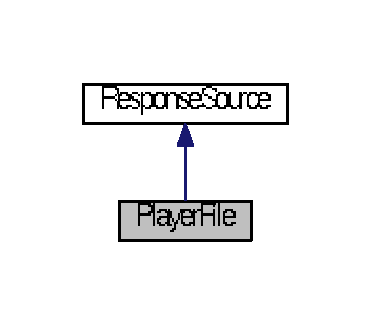
\includegraphics[width=178pt]{classPlayerFile__inherit__graph}
\end{center}
\end{figure}


Collaboration diagram for Player\+File\+:
\nopagebreak
\begin{figure}[H]
\begin{center}
\leavevmode
\includegraphics[width=350pt]{classPlayerFile__coll__graph}
\end{center}
\end{figure}
\subsection*{Public Member Functions}
\begin{DoxyCompactItemize}
\item 
\hyperlink{classPlayerFile_a655a5bf6903cad650c0dc4e33a7e41a5}{Player\+File} (const \hyperlink{classAudioSystem}{Audio\+System} \&\hyperlink{classPlayerFile_a8de47bcb924e2c3e10b208a09eb3f05b}{audio\+\_\+system})
\begin{DoxyCompactList}\small\item\em Constructs a new \hyperlink{classPlayerFile}{Player\+File}. \end{DoxyCompactList}\item 
void \hyperlink{classPlayerFile_a92dd004d4ab034bf41f7d5c76847d3c2}{Load} (const std\+::string \&path)
\begin{DoxyCompactList}\small\item\em Opens a file and stores it in this \hyperlink{classPlayerFile}{Player\+File}. \end{DoxyCompactList}\item 
\hypertarget{classPlayerFile_a426f8ad29efd5e16ac7963354087d070}{void \hyperlink{classPlayerFile_a426f8ad29efd5e16ac7963354087d070}{Start} ()}\label{classPlayerFile_a426f8ad29efd5e16ac7963354087d070}

\begin{DoxyCompactList}\small\item\em Starts the current file. \end{DoxyCompactList}\item 
\hypertarget{classPlayerFile_afd4313009b5d51df0df5dc7b59ffcf13}{void \hyperlink{classPlayerFile_afd4313009b5d51df0df5dc7b59ffcf13}{Stop} ()}\label{classPlayerFile_afd4313009b5d51df0df5dc7b59ffcf13}

\begin{DoxyCompactList}\small\item\em Stops the current file. \end{DoxyCompactList}\item 
\hypertarget{classPlayerFile_a394b2e7b4f4d0baee4ff1928a36e9945}{void \hyperlink{classPlayerFile_a394b2e7b4f4d0baee4ff1928a36e9945}{Eject} ()}\label{classPlayerFile_a394b2e7b4f4d0baee4ff1928a36e9945}

\begin{DoxyCompactList}\small\item\em Ejects the current file. \end{DoxyCompactList}\item 
void \hyperlink{classPlayerFile_a00f044c74d07d778532953a917c24197}{Emit} (\hyperlink{classResponseSink}{Response\+Sink} \&sink) const override
\begin{DoxyCompactList}\small\item\em Emits the current filename to a \hyperlink{classResponseSink}{Response\+Sink}. \end{DoxyCompactList}\item 
bool \hyperlink{classPlayerFile_a43d903e65213d3a6b2c8b38924c83c5f}{Is\+Stopped} ()
\begin{DoxyCompactList}\small\item\em Checks to see if the file has stopped playing. \end{DoxyCompactList}\item 
\hypertarget{classPlayerFile_afe0b43a6980e548a6faa87f84d22d65b}{void \hyperlink{classPlayerFile_afe0b43a6980e548a6faa87f84d22d65b}{Update} ()}\label{classPlayerFile_afe0b43a6980e548a6faa87f84d22d65b}

\begin{DoxyCompactList}\small\item\em Updates the file (performing a round of decoding on it, etc.). \end{DoxyCompactList}\item 
{\footnotesize template$<$typename R $>$ }\\R \hyperlink{classPlayerFile_a072d9788c1449e0e2de3e28b169f2c34}{Current\+Position} ()
\begin{DoxyCompactList}\small\item\em Return the current position, as a std\+::chrono\+::duration. \end{DoxyCompactList}\item 
{\footnotesize template$<$typename R $>$ }\\void \hyperlink{classPlayerFile_a8c270134404d83fe6c9e844abeacf3e5}{Seek\+To\+Position} (R position)
\begin{DoxyCompactList}\small\item\em Seek to a position expressed as a std\+::chrono\+::duration. \end{DoxyCompactList}\end{DoxyCompactItemize}
\subsection*{Private Attributes}
\begin{DoxyCompactItemize}
\item 
\hypertarget{classPlayerFile_a649de02845f72a9d326b5942596ecd6b}{std\+::unique\+\_\+ptr$<$ \hyperlink{classAudio}{Audio} $>$ \hyperlink{classPlayerFile_a649de02845f72a9d326b5942596ecd6b}{audio}}\label{classPlayerFile_a649de02845f72a9d326b5942596ecd6b}

\begin{DoxyCompactList}\small\item\em The audio file. \end{DoxyCompactList}\item 
\hypertarget{classPlayerFile_a8de47bcb924e2c3e10b208a09eb3f05b}{const \hyperlink{classAudioSystem}{Audio\+System} \& \hyperlink{classPlayerFile_a8de47bcb924e2c3e10b208a09eb3f05b}{audio\+\_\+system}}\label{classPlayerFile_a8de47bcb924e2c3e10b208a09eb3f05b}

\begin{DoxyCompactList}\small\item\em The audio system responsible for creating audio files. \end{DoxyCompactList}\end{DoxyCompactItemize}
\subsection*{Additional Inherited Members}


\subsection{Detailed Description}
The subcomponent of a \hyperlink{classPlayer}{Player} that stores the audio file. 

\begin{DoxySeeAlso}{See also}
\hyperlink{classPlayer}{Player} 
\end{DoxySeeAlso}


Definition at line \hyperlink{player__file_8hpp_source_l00024}{24} of file \hyperlink{player__file_8hpp_source}{player\+\_\+file.\+hpp}.



\subsection{Constructor \& Destructor Documentation}
\hypertarget{classPlayerFile_a655a5bf6903cad650c0dc4e33a7e41a5}{\index{Player\+File@{Player\+File}!Player\+File@{Player\+File}}
\index{Player\+File@{Player\+File}!Player\+File@{Player\+File}}
\subsubsection[{Player\+File}]{\setlength{\rightskip}{0pt plus 5cm}Player\+File\+::\+Player\+File (
\begin{DoxyParamCaption}
\item[{const {\bf Audio\+System} \&}]{audio\+\_\+system}
\end{DoxyParamCaption}
)}}\label{classPlayerFile_a655a5bf6903cad650c0dc4e33a7e41a5}


Constructs a new \hyperlink{classPlayerFile}{Player\+File}. 


\begin{DoxyParams}{Parameters}
{\em audio\+\_\+system} & The audio system to use when loading \hyperlink{classAudio}{Audio}. \\
\hline
\end{DoxyParams}


Definition at line \hyperlink{player__file_8cpp_source_l00013}{13} of file \hyperlink{player__file_8cpp_source}{player\+\_\+file.\+cpp}.


\begin{DoxyCode}
00014     : \hyperlink{classPlayerFile_a649de02845f72a9d326b5942596ecd6b}{audio}(\textcolor{keyword}{nullptr}), \hyperlink{classPlayerFile_a8de47bcb924e2c3e10b208a09eb3f05b}{audio\_system}(audio\_system)
00015 \{
00016 \}
\end{DoxyCode}


\subsection{Member Function Documentation}
\hypertarget{classPlayerFile_a072d9788c1449e0e2de3e28b169f2c34}{\index{Player\+File@{Player\+File}!Current\+Position@{Current\+Position}}
\index{Current\+Position@{Current\+Position}!Player\+File@{Player\+File}}
\subsubsection[{Current\+Position}]{\setlength{\rightskip}{0pt plus 5cm}template$<$typename R $>$ R Player\+File\+::\+Current\+Position (
\begin{DoxyParamCaption}
{}
\end{DoxyParamCaption}
)\hspace{0.3cm}{\ttfamily [inline]}}}\label{classPlayerFile_a072d9788c1449e0e2de3e28b169f2c34}


Return the current position, as a std\+::chrono\+::duration. 

\begin{DoxyReturn}{Returns}
The current position in the audio. 
\end{DoxyReturn}


Definition at line \hyperlink{player__file_8hpp_source_l00071}{71} of file \hyperlink{player__file_8hpp_source}{player\+\_\+file.\+hpp}.



References \hyperlink{player__file_8hpp_source_l00088}{audio}.



Referenced by \hyperlink{player__position_8cpp_source_l00026}{Player\+::\+Update\+Position()}.


\begin{DoxyCode}
00072     \{
00073         \textcolor{keywordflow}{return} this->\hyperlink{classPlayerFile_a649de02845f72a9d326b5942596ecd6b}{audio}->CurrentPosition<R>();
00074     \}
\end{DoxyCode}
\hypertarget{classPlayerFile_a00f044c74d07d778532953a917c24197}{\index{Player\+File@{Player\+File}!Emit@{Emit}}
\index{Emit@{Emit}!Player\+File@{Player\+File}}
\subsubsection[{Emit}]{\setlength{\rightskip}{0pt plus 5cm}void Player\+File\+::\+Emit (
\begin{DoxyParamCaption}
\item[{{\bf Response\+Sink} \&}]{sink}
\end{DoxyParamCaption}
) const\hspace{0.3cm}{\ttfamily [override]}, {\ttfamily [virtual]}}}\label{classPlayerFile_a00f044c74d07d778532953a917c24197}


Emits the current filename to a \hyperlink{classResponseSink}{Response\+Sink}. 


\begin{DoxyParams}{Parameters}
{\em sink} & The \hyperlink{classResponseSink}{Response\+Sink} to which a F\+I\+L\+E response shall be sent. \\
\hline
\end{DoxyParams}


Implements \hyperlink{classResponseSource_a498ee53cca912cdb6d48043108c39dc1}{Response\+Source}.



Definition at line \hyperlink{player__file_8cpp_source_l00018}{18} of file \hyperlink{player__file_8cpp_source}{player\+\_\+file.\+cpp}.



References \hyperlink{player__file_8hpp_source_l00088}{audio}, \hyperlink{io__response_8hpp_af5828b68a5f305a17b90321710d9b546a9fc5887c030f7a3e19821ebec457e719}{F\+I\+L\+E}, and \hyperlink{io__response_8cpp_source_l00025}{Response\+Sink\+::\+Respond()}.



Referenced by \hyperlink{player_8cpp_source_l00058}{Player\+::\+Welcome\+Client()}.


\begin{DoxyCode}
00019 \{
00020     \textcolor{keywordflow}{if} (this->\hyperlink{classPlayerFile_a649de02845f72a9d326b5942596ecd6b}{audio} != \textcolor{keyword}{nullptr}) \{
00021         sink.\hyperlink{classResponseSink_ac2add6144c2804a6f0db34ad30046ed7}{Respond}(\hyperlink{io__response_8hpp_af5828b68a5f305a17b90321710d9b546a9fc5887c030f7a3e19821ebec457e719}{ResponseCode::FILE}, this->\hyperlink{classPlayerFile_a649de02845f72a9d326b5942596ecd6b}{audio}->Path());
00022     \}
00023 \}
\end{DoxyCode}
\hypertarget{classPlayerFile_a43d903e65213d3a6b2c8b38924c83c5f}{\index{Player\+File@{Player\+File}!Is\+Stopped@{Is\+Stopped}}
\index{Is\+Stopped@{Is\+Stopped}!Player\+File@{Player\+File}}
\subsubsection[{Is\+Stopped}]{\setlength{\rightskip}{0pt plus 5cm}bool Player\+File\+::\+Is\+Stopped (
\begin{DoxyParamCaption}
{}
\end{DoxyParamCaption}
)}}\label{classPlayerFile_a43d903e65213d3a6b2c8b38924c83c5f}


Checks to see if the file has stopped playing. 

\begin{DoxyReturn}{Returns}
True if the file has stopped; false otherwise. 
\end{DoxyReturn}
\begin{DoxySeeAlso}{See also}
\hyperlink{classPlayerFile_a426f8ad29efd5e16ac7963354087d070}{Start} 

\hyperlink{classPlayerFile_afd4313009b5d51df0df5dc7b59ffcf13}{Stop} 
\end{DoxySeeAlso}


Definition at line \hyperlink{player__file_8cpp_source_l00056}{56} of file \hyperlink{player__file_8cpp_source}{player\+\_\+file.\+cpp}.



References \hyperlink{player__file_8hpp_source_l00088}{audio}.



Referenced by \hyperlink{player_8cpp_source_l00045}{Player\+::\+Playback\+Update()}.


\begin{DoxyCode}
00057 \{
00058     assert(this->\hyperlink{classPlayerFile_a649de02845f72a9d326b5942596ecd6b}{audio} != \textcolor{keyword}{nullptr});
00059     \textcolor{keywordflow}{return} this->\hyperlink{classPlayerFile_a649de02845f72a9d326b5942596ecd6b}{audio}->IsStopped();
00060 \}
\end{DoxyCode}
\hypertarget{classPlayerFile_a92dd004d4ab034bf41f7d5c76847d3c2}{\index{Player\+File@{Player\+File}!Load@{Load}}
\index{Load@{Load}!Player\+File@{Player\+File}}
\subsubsection[{Load}]{\setlength{\rightskip}{0pt plus 5cm}void Player\+File\+::\+Load (
\begin{DoxyParamCaption}
\item[{const std\+::string \&}]{path}
\end{DoxyParamCaption}
)}}\label{classPlayerFile_a92dd004d4ab034bf41f7d5c76847d3c2}


Opens a file and stores it in this \hyperlink{classPlayerFile}{Player\+File}. 


\begin{DoxyParams}{Parameters}
{\em path} & The absolute path to a track to load. \\
\hline
\end{DoxyParams}


Definition at line \hyperlink{player__file_8cpp_source_l00025}{25} of file \hyperlink{player__file_8cpp_source}{player\+\_\+file.\+cpp}.



References \hyperlink{player__file_8hpp_source_l00088}{audio}, \hyperlink{player__file_8hpp_source_l00091}{audio\+\_\+system}, \hyperlink{player__file_8cpp_source_l00033}{Eject()}, and \hyperlink{audio__system_8cpp_source_l00083}{Audio\+System\+::\+Load()}.



Referenced by \hyperlink{player_8cpp_source_l00089}{Player\+::\+Load()}.


\begin{DoxyCode}
00026 \{
00027     \textcolor{keywordflow}{if} (this->\hyperlink{classPlayerFile_a649de02845f72a9d326b5942596ecd6b}{audio} != \textcolor{keyword}{nullptr}) \{
00028         \hyperlink{classPlayerFile_a394b2e7b4f4d0baee4ff1928a36e9945}{Eject}();
00029     \}
00030     this->\hyperlink{classPlayerFile_a649de02845f72a9d326b5942596ecd6b}{audio} = decltype(this->\hyperlink{classPlayerFile_a649de02845f72a9d326b5942596ecd6b}{audio})(this->\hyperlink{classPlayerFile_a8de47bcb924e2c3e10b208a09eb3f05b}{audio\_system}.
      \hyperlink{classAudioSystem_a2172608177d2bd54377bfc3c61cd117d}{Load}(path));
00031 \}
\end{DoxyCode}
\hypertarget{classPlayerFile_a8c270134404d83fe6c9e844abeacf3e5}{\index{Player\+File@{Player\+File}!Seek\+To\+Position@{Seek\+To\+Position}}
\index{Seek\+To\+Position@{Seek\+To\+Position}!Player\+File@{Player\+File}}
\subsubsection[{Seek\+To\+Position}]{\setlength{\rightskip}{0pt plus 5cm}template$<$typename R $>$ void Player\+File\+::\+Seek\+To\+Position (
\begin{DoxyParamCaption}
\item[{R}]{position}
\end{DoxyParamCaption}
)\hspace{0.3cm}{\ttfamily [inline]}}}\label{classPlayerFile_a8c270134404d83fe6c9e844abeacf3e5}


Seek to a position expressed as a std\+::chrono\+::duration. 


\begin{DoxyParams}{Parameters}
{\em position} & The position to seek to in the audio. \\
\hline
\end{DoxyParams}


Definition at line \hyperlink{player__file_8hpp_source_l00081}{81} of file \hyperlink{player__file_8hpp_source}{player\+\_\+file.\+hpp}.



References \hyperlink{player__file_8hpp_source_l00088}{audio}.



Referenced by \hyperlink{player_8cpp_source_l00134}{Player\+::\+Seek()}.


\begin{DoxyCode}
00082     \{
00083         this->\hyperlink{classPlayerFile_a649de02845f72a9d326b5942596ecd6b}{audio}->SeekToPosition<R>(position);
00084     \}
\end{DoxyCode}


The documentation for this class was generated from the following files\+:\begin{DoxyCompactItemize}
\item 
src/player/\hyperlink{player__file_8hpp}{player\+\_\+file.\+hpp}\item 
src/player/\hyperlink{player__file_8cpp}{player\+\_\+file.\+cpp}\end{DoxyCompactItemize}

\hypertarget{classPlayerPosition}{\section{Player\+Position Class Reference}
\label{classPlayerPosition}\index{Player\+Position@{Player\+Position}}
}


Tracker and broadcaster for the \hyperlink{classPlayer}{Player}'s current position in a song.  




{\ttfamily \#include $<$player\+\_\+position.\+hpp$>$}



Inheritance diagram for Player\+Position\+:
\nopagebreak
\begin{figure}[H]
\begin{center}
\leavevmode
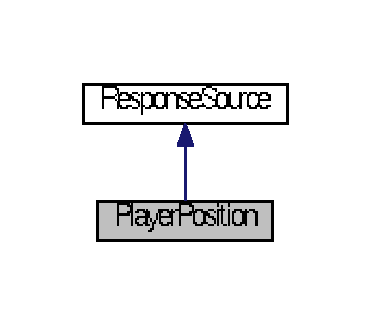
\includegraphics[width=178pt]{classPlayerPosition__inherit__graph}
\end{center}
\end{figure}


Collaboration diagram for Player\+Position\+:
\nopagebreak
\begin{figure}[H]
\begin{center}
\leavevmode
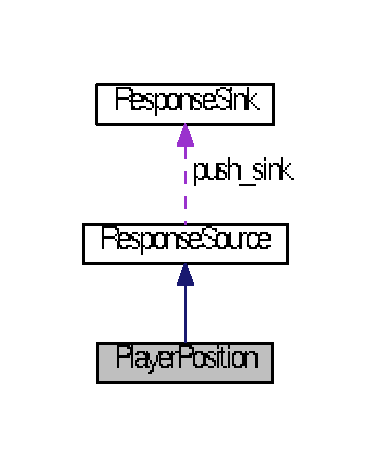
\includegraphics[width=180pt]{classPlayerPosition__coll__graph}
\end{center}
\end{figure}
\subsection*{Public Types}
\begin{DoxyCompactItemize}
\item 
\hypertarget{classPlayerPosition_a535c99057ceca21d8fbe82883c592a66}{using \hyperlink{classPlayerPosition_a535c99057ceca21d8fbe82883c592a66}{Unit} = std\+::chrono\+::microseconds}\label{classPlayerPosition_a535c99057ceca21d8fbe82883c592a66}

\begin{DoxyCompactList}\small\item\em Unit used for positions. \end{DoxyCompactList}\end{DoxyCompactItemize}
\subsection*{Public Member Functions}
\begin{DoxyCompactItemize}
\item 
\hypertarget{classPlayerPosition_a707498560b9f9189fb6d3cd8e59b77d7}{\hyperlink{classPlayerPosition_a707498560b9f9189fb6d3cd8e59b77d7}{Player\+Position} ()}\label{classPlayerPosition_a707498560b9f9189fb6d3cd8e59b77d7}

\begin{DoxyCompactList}\small\item\em Constructs a \hyperlink{classPlayerPosition}{Player\+Position}. \end{DoxyCompactList}\item 
void \hyperlink{classPlayerPosition_aee2fec4f9cd5db48ee1ed79044c658ab}{Set\+Response\+Period} (\hyperlink{classPlayerPosition_a535c99057ceca21d8fbe82883c592a66}{Unit} \hyperlink{classPlayerPosition_a59fceae86a59fb8ad1fb4e93160f948c}{period})
\begin{DoxyCompactList}\small\item\em Sets the period between position signals. \end{DoxyCompactList}\item 
void \hyperlink{classPlayerPosition_ad39cab72590804238d2384391cb65745}{Update} (\hyperlink{classPlayerPosition_a535c99057ceca21d8fbe82883c592a66}{Unit} position)
\begin{DoxyCompactList}\small\item\em Updates the position tracker with the new position. \end{DoxyCompactList}\item 
void \hyperlink{classPlayerPosition_a813e8eb40fdff815683fb7a5b1671ede}{Reset} ()
\begin{DoxyCompactList}\small\item\em Resets the position tracker's position data. \end{DoxyCompactList}\item 
void \hyperlink{classPlayerPosition_a66963c28fd9dffe0fd7338023310fa92}{Emit} (\hyperlink{classResponseSink}{Response\+Sink} \&sink) const override
\begin{DoxyCompactList}\small\item\em Emits the current position to a \hyperlink{classResponseSink}{Response\+Sink}. \end{DoxyCompactList}\end{DoxyCompactItemize}
\subsection*{Private Member Functions}
\begin{DoxyCompactItemize}
\item 
bool \hyperlink{classPlayerPosition_a52f46d4c600724b7ce9f459b93609dc3}{Is\+Ready\+To\+Send} ()
\begin{DoxyCompactList}\small\item\em Figures out whether it's time to send a position signal. \end{DoxyCompactList}\item 
void \hyperlink{classPlayerPosition_aac73ce9104537702365baf19d50bde14}{Send} ()
\begin{DoxyCompactList}\small\item\em Sends a position signal to the outside environment, if ready. \end{DoxyCompactList}\end{DoxyCompactItemize}
\subsection*{Private Attributes}
\begin{DoxyCompactItemize}
\item 
\hypertarget{classPlayerPosition_a59fceae86a59fb8ad1fb4e93160f948c}{\hyperlink{classPlayerPosition_a535c99057ceca21d8fbe82883c592a66}{Unit} \hyperlink{classPlayerPosition_a59fceae86a59fb8ad1fb4e93160f948c}{period}}\label{classPlayerPosition_a59fceae86a59fb8ad1fb4e93160f948c}

\begin{DoxyCompactList}\small\item\em The period between each push of the position to the response sink. \end{DoxyCompactList}\item 
\hypertarget{classPlayerPosition_a043f477d249cca2eaa00e0e616888bea}{\hyperlink{classPlayerPosition_a535c99057ceca21d8fbe82883c592a66}{Unit} \hyperlink{classPlayerPosition_a043f477d249cca2eaa00e0e616888bea}{current}}\label{classPlayerPosition_a043f477d249cca2eaa00e0e616888bea}

\begin{DoxyCompactList}\small\item\em The current position of the player. \end{DoxyCompactList}\item 
\hypertarget{classPlayerPosition_a4adeb717201c469c16236c2d2d6f9cef}{\hyperlink{classPlayerPosition_a535c99057ceca21d8fbe82883c592a66}{Unit} \hyperlink{classPlayerPosition_a4adeb717201c469c16236c2d2d6f9cef}{last}}\label{classPlayerPosition_a4adeb717201c469c16236c2d2d6f9cef}

\begin{DoxyCompactList}\small\item\em The position of the player at the last push. \end{DoxyCompactList}\item 
bool \hyperlink{classPlayerPosition_a876749ea389ec23a8af6fe26e3e13883}{has\+\_\+reset}
\begin{DoxyCompactList}\small\item\em Whether the position was reset since the last push. \end{DoxyCompactList}\end{DoxyCompactItemize}
\subsection*{Additional Inherited Members}


\subsection{Detailed Description}
Tracker and broadcaster for the \hyperlink{classPlayer}{Player}'s current position in a song. 

\begin{DoxySeeAlso}{See also}
\hyperlink{classPlayer}{Player} 

\hyperlink{classPlayerState}{Player\+State} 
\end{DoxySeeAlso}


Definition at line \hyperlink{player__position_8hpp_source_l00024}{24} of file \hyperlink{player__position_8hpp_source}{player\+\_\+position.\+hpp}.



\subsection{Member Function Documentation}
\hypertarget{classPlayerPosition_a66963c28fd9dffe0fd7338023310fa92}{\index{Player\+Position@{Player\+Position}!Emit@{Emit}}
\index{Emit@{Emit}!Player\+Position@{Player\+Position}}
\subsubsection[{Emit}]{\setlength{\rightskip}{0pt plus 5cm}void Player\+Position\+::\+Emit (
\begin{DoxyParamCaption}
\item[{{\bf Response\+Sink} \&}]{sink}
\end{DoxyParamCaption}
) const\hspace{0.3cm}{\ttfamily [override]}, {\ttfamily [virtual]}}}\label{classPlayerPosition_a66963c28fd9dffe0fd7338023310fa92}


Emits the current position to a \hyperlink{classResponseSink}{Response\+Sink}. 


\begin{DoxyParams}{Parameters}
{\em sink} & The \hyperlink{classResponseSink}{Response\+Sink} to which a T\+I\+M\+E response shall be sent. \\
\hline
\end{DoxyParams}


Implements \hyperlink{classResponseSource_a498ee53cca912cdb6d48043108c39dc1}{Response\+Source}.



Definition at line \hyperlink{player__position_8cpp_source_l00067}{67} of file \hyperlink{player__position_8cpp_source}{player\+\_\+position.\+cpp}.



References \hyperlink{player__position_8hpp_source_l00034}{current}, \hyperlink{io__response_8cpp_source_l00025}{Response\+Sink\+::\+Respond()}, and \hyperlink{io__response_8hpp_af5828b68a5f305a17b90321710d9b546a346ff32eaa3c09983fb2ec057816d352}{T\+I\+M\+E}.



Referenced by \hyperlink{player_8cpp_source_l00058}{Player\+::\+Welcome\+Client()}.


\begin{DoxyCode}
00068 \{
00069     std::ostringstream os;
00070     os << this->\hyperlink{classPlayerPosition_a043f477d249cca2eaa00e0e616888bea}{current}.count();
00071 
00072     target.Respond(\hyperlink{io__response_8hpp_af5828b68a5f305a17b90321710d9b546a346ff32eaa3c09983fb2ec057816d352}{ResponseCode::TIME}, os.str());
00073 \}
\end{DoxyCode}
\hypertarget{classPlayerPosition_a52f46d4c600724b7ce9f459b93609dc3}{\index{Player\+Position@{Player\+Position}!Is\+Ready\+To\+Send@{Is\+Ready\+To\+Send}}
\index{Is\+Ready\+To\+Send@{Is\+Ready\+To\+Send}!Player\+Position@{Player\+Position}}
\subsubsection[{Is\+Ready\+To\+Send}]{\setlength{\rightskip}{0pt plus 5cm}bool Player\+Position\+::\+Is\+Ready\+To\+Send (
\begin{DoxyParamCaption}
{}
\end{DoxyParamCaption}
)\hspace{0.3cm}{\ttfamily [private]}}}\label{classPlayerPosition_a52f46d4c600724b7ce9f459b93609dc3}


Figures out whether it's time to send a position signal. 

\begin{DoxyReturn}{Returns}
True if enough time has elapsed for a signal to be sent; false otherwise. 
\end{DoxyReturn}


Definition at line \hyperlink{player__position_8cpp_source_l00075}{75} of file \hyperlink{player__position_8cpp_source}{player\+\_\+position.\+cpp}.



References \hyperlink{player__position_8hpp_source_l00034}{current}, \hyperlink{player__position_8hpp_source_l00043}{has\+\_\+reset}, \hyperlink{player__position_8hpp_source_l00037}{last}, and \hyperlink{player__position_8hpp_source_l00031}{period}.



Referenced by \hyperlink{player__position_8cpp_source_l00049}{Update()}.


\begin{DoxyCode}
00076 \{
00077     \textcolor{keywordflow}{return} this->\hyperlink{classPlayerPosition_a876749ea389ec23a8af6fe26e3e13883}{has\_reset} || (this->\hyperlink{classPlayerPosition_a4adeb717201c469c16236c2d2d6f9cef}{last} + this->\hyperlink{classPlayerPosition_a59fceae86a59fb8ad1fb4e93160f948c}{period} <= this->
      \hyperlink{classPlayerPosition_a043f477d249cca2eaa00e0e616888bea}{current});
00078 \}
\end{DoxyCode}
\hypertarget{classPlayerPosition_a813e8eb40fdff815683fb7a5b1671ede}{\index{Player\+Position@{Player\+Position}!Reset@{Reset}}
\index{Reset@{Reset}!Player\+Position@{Player\+Position}}
\subsubsection[{Reset}]{\setlength{\rightskip}{0pt plus 5cm}void Player\+Position\+::\+Reset (
\begin{DoxyParamCaption}
{}
\end{DoxyParamCaption}
)}}\label{classPlayerPosition_a813e8eb40fdff815683fb7a5b1671ede}


Resets the position tracker's position data. 

This does not remove any registered push response sink. Call this whenever the song changes, or before a skip. \begin{DoxySeeAlso}{See also}
\hyperlink{classPlayerPosition_ad39cab72590804238d2384391cb65745}{Update} 
\end{DoxySeeAlso}


Definition at line \hyperlink{player__position_8cpp_source_l00060}{60} of file \hyperlink{player__position_8cpp_source}{player\+\_\+position.\+cpp}.



References \hyperlink{player__position_8hpp_source_l00034}{current}, \hyperlink{player__position_8hpp_source_l00043}{has\+\_\+reset}, and \hyperlink{player__position_8hpp_source_l00037}{last}.



Referenced by \hyperlink{player__position_8cpp_source_l00041}{Player\+Position()}, and \hyperlink{player__position_8cpp_source_l00032}{Player\+::\+Reset\+Position()}.


\begin{DoxyCode}
00061 \{
00062     this->\hyperlink{classPlayerPosition_a043f477d249cca2eaa00e0e616888bea}{current} = \hyperlink{classPlayerPosition_a535c99057ceca21d8fbe82883c592a66}{Unit}(0);
00063     this->\hyperlink{classPlayerPosition_a4adeb717201c469c16236c2d2d6f9cef}{last} = \hyperlink{classPlayerPosition_a535c99057ceca21d8fbe82883c592a66}{Unit}(0);
00064     this->\hyperlink{classPlayerPosition_a876749ea389ec23a8af6fe26e3e13883}{has\_reset} = \textcolor{keyword}{true};
00065 \}
\end{DoxyCode}
\hypertarget{classPlayerPosition_aac73ce9104537702365baf19d50bde14}{\index{Player\+Position@{Player\+Position}!Send@{Send}}
\index{Send@{Send}!Player\+Position@{Player\+Position}}
\subsubsection[{Send}]{\setlength{\rightskip}{0pt plus 5cm}void Player\+Position\+::\+Send (
\begin{DoxyParamCaption}
{}
\end{DoxyParamCaption}
)\hspace{0.3cm}{\ttfamily [private]}}}\label{classPlayerPosition_aac73ce9104537702365baf19d50bde14}


Sends a position signal to the outside environment, if ready. 

This only sends a signal if the requested amount of time has passed since the last one. \hypertarget{classPlayerPosition_aee2fec4f9cd5db48ee1ed79044c658ab}{\index{Player\+Position@{Player\+Position}!Set\+Response\+Period@{Set\+Response\+Period}}
\index{Set\+Response\+Period@{Set\+Response\+Period}!Player\+Position@{Player\+Position}}
\subsubsection[{Set\+Response\+Period}]{\setlength{\rightskip}{0pt plus 5cm}void Player\+Position\+::\+Set\+Response\+Period (
\begin{DoxyParamCaption}
\item[{{\bf Player\+Position\+::\+Unit}}]{period}
\end{DoxyParamCaption}
)}}\label{classPlayerPosition_aee2fec4f9cd5db48ee1ed79044c658ab}


Sets the period between position signals. 

This is shared across all listeners. 
\begin{DoxyParams}{Parameters}
{\em period} & The period to wait between responses. \\
\hline
\end{DoxyParams}
\begin{DoxySeeAlso}{See also}
\hyperlink{classResponseSource_a12c45136716adffa59d5e5e1ca80b7ce}{Set\+Response\+Sink} 
\end{DoxySeeAlso}


Definition at line \hyperlink{player__position_8cpp_source_l00080}{80} of file \hyperlink{player__position_8cpp_source}{player\+\_\+position.\+cpp}.



References \hyperlink{player__position_8hpp_source_l00031}{period}.



Referenced by \hyperlink{player__position_8cpp_source_l00021}{Player\+::\+Set\+Position\+Response\+Period()}.


\begin{DoxyCode}
00081 \{
00082     this->\hyperlink{classPlayerPosition_a59fceae86a59fb8ad1fb4e93160f948c}{period} = \hyperlink{classPlayerPosition_a59fceae86a59fb8ad1fb4e93160f948c}{period};
00083 \}
\end{DoxyCode}
\hypertarget{classPlayerPosition_ad39cab72590804238d2384391cb65745}{\index{Player\+Position@{Player\+Position}!Update@{Update}}
\index{Update@{Update}!Player\+Position@{Player\+Position}}
\subsubsection[{Update}]{\setlength{\rightskip}{0pt plus 5cm}void Player\+Position\+::\+Update (
\begin{DoxyParamCaption}
\item[{const {\bf Player\+Position\+::\+Unit}}]{position}
\end{DoxyParamCaption}
)}}\label{classPlayerPosition_ad39cab72590804238d2384391cb65745}


Updates the position tracker with the new position. 

This pushes the position to the registered response sink, if necessary. 
\begin{DoxyParams}{Parameters}
{\em position} & The new position, in {\itshape Position\+Unit} units. \\
\hline
\end{DoxyParams}
\begin{DoxySeeAlso}{See also}
\hyperlink{classPlayerPosition_a813e8eb40fdff815683fb7a5b1671ede}{Reset} 
\end{DoxySeeAlso}


Definition at line \hyperlink{player__position_8cpp_source_l00049}{49} of file \hyperlink{player__position_8cpp_source}{player\+\_\+position.\+cpp}.



References \hyperlink{player__position_8hpp_source_l00034}{current}, \hyperlink{player__position_8hpp_source_l00043}{has\+\_\+reset}, \hyperlink{player__position_8cpp_source_l00075}{Is\+Ready\+To\+Send()}, \hyperlink{player__position_8hpp_source_l00037}{last}, and \hyperlink{io__response_8cpp_source_l00047}{Response\+Source\+::\+Push()}.



Referenced by \hyperlink{player__position_8cpp_source_l00026}{Player\+::\+Update\+Position()}.


\begin{DoxyCode}
00050 \{
00051     this->\hyperlink{classPlayerPosition_a043f477d249cca2eaa00e0e616888bea}{current} = position;
00052 
00053     \textcolor{keywordflow}{if} (\hyperlink{classPlayerPosition_a52f46d4c600724b7ce9f459b93609dc3}{IsReadyToSend}()) \{
00054         \hyperlink{classResponseSource_a6e3b93326ee043f6d60510acd08de69b}{Push}();
00055         this->\hyperlink{classPlayerPosition_a4adeb717201c469c16236c2d2d6f9cef}{last} = this->\hyperlink{classPlayerPosition_a043f477d249cca2eaa00e0e616888bea}{current};
00056         this->\hyperlink{classPlayerPosition_a876749ea389ec23a8af6fe26e3e13883}{has\_reset} = 0;
00057     \}
00058 \}
\end{DoxyCode}


\subsection{Member Data Documentation}
\hypertarget{classPlayerPosition_a876749ea389ec23a8af6fe26e3e13883}{\index{Player\+Position@{Player\+Position}!has\+\_\+reset@{has\+\_\+reset}}
\index{has\+\_\+reset@{has\+\_\+reset}!Player\+Position@{Player\+Position}}
\subsubsection[{has\+\_\+reset}]{\setlength{\rightskip}{0pt plus 5cm}bool Player\+Position\+::has\+\_\+reset\hspace{0.3cm}{\ttfamily [private]}}}\label{classPlayerPosition_a876749ea389ec23a8af6fe26e3e13883}


Whether the position was reset since the last push. 

This is also set high if the position has never been emitted. 

Definition at line \hyperlink{player__position_8hpp_source_l00043}{43} of file \hyperlink{player__position_8hpp_source}{player\+\_\+position.\+hpp}.



Referenced by \hyperlink{player__position_8cpp_source_l00075}{Is\+Ready\+To\+Send()}, \hyperlink{player__position_8cpp_source_l00060}{Reset()}, and \hyperlink{player__position_8cpp_source_l00049}{Update()}.



The documentation for this class was generated from the following files\+:\begin{DoxyCompactItemize}
\item 
src/player/\hyperlink{player__position_8hpp}{player\+\_\+position.\+hpp}\item 
src/player/\hyperlink{player__position_8cpp}{player\+\_\+position.\+cpp}\end{DoxyCompactItemize}

\hypertarget{classPlayerState}{\section{Player\+State Class Reference}
\label{classPlayerState}\index{Player\+State@{Player\+State}}
}


An object holding and representing the current state of a \hyperlink{classPlayer}{Player}.  




{\ttfamily \#include $<$player\+\_\+state.\+hpp$>$}



Inheritance diagram for Player\+State\+:
\nopagebreak
\begin{figure}[H]
\begin{center}
\leavevmode
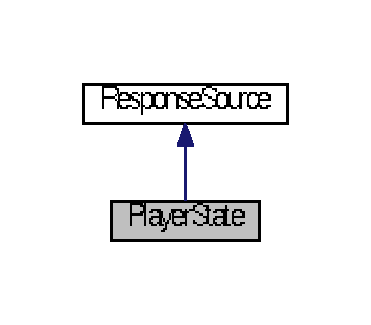
\includegraphics[width=178pt]{classPlayerState__inherit__graph}
\end{center}
\end{figure}


Collaboration diagram for Player\+State\+:
\nopagebreak
\begin{figure}[H]
\begin{center}
\leavevmode
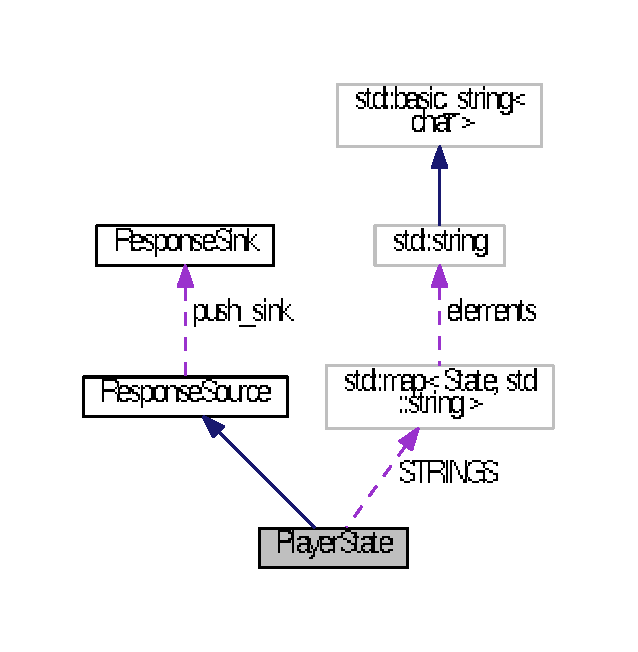
\includegraphics[width=306pt]{classPlayerState__coll__graph}
\end{center}
\end{figure}
\subsection*{Public Types}
\begin{DoxyCompactItemize}
\item 
enum \hyperlink{classPlayerState_ab013f68ff23d69d677faae624b5dff07}{State} \+: std\+::uint8\+\_\+t \{ \\*
\hyperlink{classPlayerState_ab013f68ff23d69d677faae624b5dff07a034312d8adc8099c1c6f53aaff745e26}{State\+::\+S\+T\+A\+R\+T\+I\+N\+G}, 
\hyperlink{classPlayerState_ab013f68ff23d69d677faae624b5dff07a209d5541434371bb6b79dc8cca8fa55b}{State\+::\+E\+J\+E\+C\+T\+E\+D}, 
\hyperlink{classPlayerState_ab013f68ff23d69d677faae624b5dff07a09d4d696b4e935115b9313e3c412509a}{State\+::\+S\+T\+O\+P\+P\+E\+D}, 
\hyperlink{classPlayerState_ab013f68ff23d69d677faae624b5dff07a50366a49630a416ab3ccaa004196027e}{State\+::\+P\+L\+A\+Y\+I\+N\+G}, 
\\*
\hyperlink{classPlayerState_ab013f68ff23d69d677faae624b5dff07a4eb3979af877a3c13830cd69c746e230}{State\+::\+Q\+U\+I\+T\+T\+I\+N\+G}
 \}
\begin{DoxyCompactList}\small\item\em Enumeration of states that the player can be in. \end{DoxyCompactList}\item 
\hypertarget{classPlayerState_a0f4e455f0579f97740855ccc6177c9f1}{using \hyperlink{classPlayerState_a0f4e455f0579f97740855ccc6177c9f1}{List} = std\+::initializer\+\_\+list$<$ \hyperlink{classPlayerState_ab013f68ff23d69d677faae624b5dff07}{State} $>$}\label{classPlayerState_a0f4e455f0579f97740855ccc6177c9f1}

\begin{DoxyCompactList}\small\item\em A list of states, used for If\+In. \end{DoxyCompactList}\end{DoxyCompactItemize}
\subsection*{Public Member Functions}
\begin{DoxyCompactItemize}
\item 
\hypertarget{classPlayerState_a6d3de3f57e9db4ec34e5a7403fc03868}{\hyperlink{classPlayerState_a6d3de3f57e9db4ec34e5a7403fc03868}{Player\+State} ()}\label{classPlayerState_a6d3de3f57e9db4ec34e5a7403fc03868}

\begin{DoxyCompactList}\small\item\em Constructs a \hyperlink{classPlayerState}{Player\+State}. \end{DoxyCompactList}\item 
void \hyperlink{classPlayerState_aa93a9879688bfbd3d89ac102c079cbfd}{Emit} (\hyperlink{classResponseSink}{Response\+Sink} \&sink) const override
\begin{DoxyCompactList}\small\item\em Announces the current state to a \hyperlink{classResponseSink}{Response\+Sink}. \end{DoxyCompactList}\item 
bool \hyperlink{classPlayerState_aa2c0e603dd57dcc37759d716596ffa33}{In} (\hyperlink{classPlayerState_a0f4e455f0579f97740855ccc6177c9f1}{List} states) const 
\begin{DoxyCompactList}\small\item\em Checks whether the current state is in a given list of states. \end{DoxyCompactList}\item 
bool \hyperlink{classPlayerState_aeb19817b9da2f6765b990983f87e1527}{Is\+Running} () const 
\begin{DoxyCompactList}\small\item\em Returns whether the player is still running. \end{DoxyCompactList}\item 
void \hyperlink{classPlayerState_a822999cf7d4cf72ba77f218906bb8aaa}{Set} (\hyperlink{classPlayerState_ab013f68ff23d69d677faae624b5dff07}{State} state)
\begin{DoxyCompactList}\small\item\em Sets the player's current state. \end{DoxyCompactList}\end{DoxyCompactItemize}
\subsection*{Static Public Attributes}
\begin{DoxyCompactItemize}
\item 
static const \hyperlink{classPlayerState_a0f4e455f0579f97740855ccc6177c9f1}{List} \hyperlink{classPlayerState_aa5e7203a1fa44e8bceffe65b6ad2c554}{A\+U\+D\+I\+O\+\_\+\+P\+L\+A\+Y\+I\+N\+G\+\_\+\+S\+T\+A\+T\+E\+S}
\begin{DoxyCompactList}\small\item\em List of states in which the player is playing something. \end{DoxyCompactList}\item 
static const \hyperlink{classPlayerState_a0f4e455f0579f97740855ccc6177c9f1}{List} \hyperlink{classPlayerState_a850bf90685a377001cfc46808cf017a4}{A\+U\+D\+I\+O\+\_\+\+L\+O\+A\+D\+E\+D\+\_\+\+S\+T\+A\+T\+E\+S}
\begin{DoxyCompactList}\small\item\em List of states in which some audio is loaded. \end{DoxyCompactList}\end{DoxyCompactItemize}
\subsection*{Private Attributes}
\begin{DoxyCompactItemize}
\item 
\hypertarget{classPlayerState_add16beba271881c0e1e40430b80f5bd6}{\hyperlink{classPlayerState_ab013f68ff23d69d677faae624b5dff07}{State} \hyperlink{classPlayerState_add16beba271881c0e1e40430b80f5bd6}{current}}\label{classPlayerState_add16beba271881c0e1e40430b80f5bd6}

\begin{DoxyCompactList}\small\item\em The current state. \end{DoxyCompactList}\end{DoxyCompactItemize}
\subsection*{Static Private Attributes}
\begin{DoxyCompactItemize}
\item 
static const std\+::map$<$ \hyperlink{classPlayerState_ab013f68ff23d69d677faae624b5dff07}{State}, \\*
std\+::string $>$ \hyperlink{classPlayerState_af9cd9cd0e2d4c24e59ea11d35bdaff78}{S\+T\+R\+I\+N\+G\+S}
\begin{DoxyCompactList}\small\item\em A mapping between states and their human-\/readable names. \end{DoxyCompactList}\end{DoxyCompactItemize}
\subsection*{Additional Inherited Members}


\subsection{Detailed Description}
An object holding and representing the current state of a \hyperlink{classPlayer}{Player}. 

\begin{DoxySeeAlso}{See also}
\hyperlink{classPlayer}{Player} 

\hyperlink{classPlayerPosition}{Player\+Position} 
\end{DoxySeeAlso}


Definition at line \hyperlink{player__state_8hpp_source_l00024}{24} of file \hyperlink{player__state_8hpp_source}{player\+\_\+state.\+hpp}.



\subsection{Member Enumeration Documentation}
\hypertarget{classPlayerState_ab013f68ff23d69d677faae624b5dff07}{\index{Player\+State@{Player\+State}!State@{State}}
\index{State@{State}!Player\+State@{Player\+State}}
\subsubsection[{State}]{\setlength{\rightskip}{0pt plus 5cm}enum {\bf Player\+State\+::\+State} \+: std\+::uint8\+\_\+t\hspace{0.3cm}{\ttfamily [strong]}}}\label{classPlayerState_ab013f68ff23d69d677faae624b5dff07}


Enumeration of states that the player can be in. 

The player is effectively a finite-\/state machine whose behaviour at any given time is dictated by the current state, which is represented by an instance of State. \begin{Desc}
\item[Enumerator]\par
\begin{description}
\index{S\+T\+A\+R\+T\+I\+N\+G@{S\+T\+A\+R\+T\+I\+N\+G}!Player\+State@{Player\+State}}\index{Player\+State@{Player\+State}!S\+T\+A\+R\+T\+I\+N\+G@{S\+T\+A\+R\+T\+I\+N\+G}}\item[{\em 
\hypertarget{classPlayerState_ab013f68ff23d69d677faae624b5dff07a034312d8adc8099c1c6f53aaff745e26}{S\+T\+A\+R\+T\+I\+N\+G}\label{classPlayerState_ab013f68ff23d69d677faae624b5dff07a034312d8adc8099c1c6f53aaff745e26}
}]The player has just initialised. \index{E\+J\+E\+C\+T\+E\+D@{E\+J\+E\+C\+T\+E\+D}!Player\+State@{Player\+State}}\index{Player\+State@{Player\+State}!E\+J\+E\+C\+T\+E\+D@{E\+J\+E\+C\+T\+E\+D}}\item[{\em 
\hypertarget{classPlayerState_ab013f68ff23d69d677faae624b5dff07a209d5541434371bb6b79dc8cca8fa55b}{E\+J\+E\+C\+T\+E\+D}\label{classPlayerState_ab013f68ff23d69d677faae624b5dff07a209d5541434371bb6b79dc8cca8fa55b}
}]The player has no song loaded. \index{S\+T\+O\+P\+P\+E\+D@{S\+T\+O\+P\+P\+E\+D}!Player\+State@{Player\+State}}\index{Player\+State@{Player\+State}!S\+T\+O\+P\+P\+E\+D@{S\+T\+O\+P\+P\+E\+D}}\item[{\em 
\hypertarget{classPlayerState_ab013f68ff23d69d677faae624b5dff07a09d4d696b4e935115b9313e3c412509a}{S\+T\+O\+P\+P\+E\+D}\label{classPlayerState_ab013f68ff23d69d677faae624b5dff07a09d4d696b4e935115b9313e3c412509a}
}]The player has a song loaded and not playing. \index{P\+L\+A\+Y\+I\+N\+G@{P\+L\+A\+Y\+I\+N\+G}!Player\+State@{Player\+State}}\index{Player\+State@{Player\+State}!P\+L\+A\+Y\+I\+N\+G@{P\+L\+A\+Y\+I\+N\+G}}\item[{\em 
\hypertarget{classPlayerState_ab013f68ff23d69d677faae624b5dff07a50366a49630a416ab3ccaa004196027e}{P\+L\+A\+Y\+I\+N\+G}\label{classPlayerState_ab013f68ff23d69d677faae624b5dff07a50366a49630a416ab3ccaa004196027e}
}]The player has a song loaded and playing. \index{Q\+U\+I\+T\+T\+I\+N\+G@{Q\+U\+I\+T\+T\+I\+N\+G}!Player\+State@{Player\+State}}\index{Player\+State@{Player\+State}!Q\+U\+I\+T\+T\+I\+N\+G@{Q\+U\+I\+T\+T\+I\+N\+G}}\item[{\em 
\hypertarget{classPlayerState_ab013f68ff23d69d677faae624b5dff07a4eb3979af877a3c13830cd69c746e230}{Q\+U\+I\+T\+T\+I\+N\+G}\label{classPlayerState_ab013f68ff23d69d677faae624b5dff07a4eb3979af877a3c13830cd69c746e230}
}]The player is about to terminate. \end{description}
\end{Desc}


Definition at line \hyperlink{player__state_8hpp_source_l00032}{32} of file \hyperlink{player__state_8hpp_source}{player\+\_\+state.\+hpp}.


\begin{DoxyCode}
00032                      : std::uint8\_t \{
00033         STARTING, 
00034         EJECTED,  
00035         STOPPED,  
00036         PLAYING,  
00037         QUITTING  
00038     \};
\end{DoxyCode}


\subsection{Member Function Documentation}
\hypertarget{classPlayerState_aa93a9879688bfbd3d89ac102c079cbfd}{\index{Player\+State@{Player\+State}!Emit@{Emit}}
\index{Emit@{Emit}!Player\+State@{Player\+State}}
\subsubsection[{Emit}]{\setlength{\rightskip}{0pt plus 5cm}void Player\+State\+::\+Emit (
\begin{DoxyParamCaption}
\item[{{\bf Response\+Sink} \&}]{sink}
\end{DoxyParamCaption}
) const\hspace{0.3cm}{\ttfamily [override]}, {\ttfamily [virtual]}}}\label{classPlayerState_aa93a9879688bfbd3d89ac102c079cbfd}


Announces the current state to a \hyperlink{classResponseSink}{Response\+Sink}. 


\begin{DoxyParams}{Parameters}
{\em sink} & The \hyperlink{classResponseSink}{Response\+Sink} to which the current state shall be emitted. \\
\hline
\end{DoxyParams}


Implements \hyperlink{classResponseSource_a498ee53cca912cdb6d48043108c39dc1}{Response\+Source}.



Definition at line \hyperlink{player__state_8cpp_source_l00052}{52} of file \hyperlink{player__state_8cpp_source}{player\+\_\+state.\+cpp}.



References \hyperlink{player__state_8hpp_source_l00086}{current}, \hyperlink{io__response_8cpp_source_l00025}{Response\+Sink\+::\+Respond()}, \hyperlink{io__response_8hpp_af5828b68a5f305a17b90321710d9b546a2b848a8cc886d253d21a77c43cd50aae}{S\+T\+A\+T\+E}, and \hyperlink{player__state_8hpp_source_l00083}{S\+T\+R\+I\+N\+G\+S}.



Referenced by \hyperlink{player_8cpp_source_l00058}{Player\+::\+Welcome\+Client()}.


\begin{DoxyCode}
00053 \{
00054     responder.Respond(\hyperlink{io__response_8hpp_af5828b68a5f305a17b90321710d9b546a2b848a8cc886d253d21a77c43cd50aae}{ResponseCode::STATE},
00055                       \hyperlink{classPlayerState_af9cd9cd0e2d4c24e59ea11d35bdaff78}{PlayerState::STRINGS}.at(this->\hyperlink{classPlayerState_add16beba271881c0e1e40430b80f5bd6}{current}));
00056 \}
\end{DoxyCode}
\hypertarget{classPlayerState_aa2c0e603dd57dcc37759d716596ffa33}{\index{Player\+State@{Player\+State}!In@{In}}
\index{In@{In}!Player\+State@{Player\+State}}
\subsubsection[{In}]{\setlength{\rightskip}{0pt plus 5cm}bool Player\+State\+::\+In (
\begin{DoxyParamCaption}
\item[{{\bf Player\+State\+::\+List}}]{states}
\end{DoxyParamCaption}
) const}}\label{classPlayerState_aa2c0e603dd57dcc37759d716596ffa33}


Checks whether the current state is in a given list of states. 


\begin{DoxyParams}{Parameters}
{\em states} & The initialiser list of states. \\
\hline
\end{DoxyParams}
\begin{DoxyReturn}{Returns}
True if the state is in the List; false otherwise. 
\end{DoxyReturn}


Definition at line \hyperlink{player__state_8cpp_source_l00058}{58} of file \hyperlink{player__state_8cpp_source}{player\+\_\+state.\+cpp}.



References \hyperlink{player__state_8hpp_source_l00086}{current}.



Referenced by \hyperlink{player__state_8cpp_source_l00021}{Player\+::\+Current\+State\+In()}.


\begin{DoxyCode}
00059 \{
00060     \textcolor{keywordflow}{return} std::find(states.begin(), states.end(), this->\hyperlink{classPlayerState_add16beba271881c0e1e40430b80f5bd6}{current}) !=
00061            states.end();
00062 \}
\end{DoxyCode}
\hypertarget{classPlayerState_aeb19817b9da2f6765b990983f87e1527}{\index{Player\+State@{Player\+State}!Is\+Running@{Is\+Running}}
\index{Is\+Running@{Is\+Running}!Player\+State@{Player\+State}}
\subsubsection[{Is\+Running}]{\setlength{\rightskip}{0pt plus 5cm}bool Player\+State\+::\+Is\+Running (
\begin{DoxyParamCaption}
{}
\end{DoxyParamCaption}
) const}}\label{classPlayerState_aeb19817b9da2f6765b990983f87e1527}


Returns whether the player is still running. 

\begin{DoxyReturn}{Returns}
True if the player is not in the Q\+U\+I\+T\+T\+I\+N\+G state; false otherwise. 
\end{DoxyReturn}


Definition at line \hyperlink{player__state_8cpp_source_l00064}{64} of file \hyperlink{player__state_8cpp_source}{player\+\_\+state.\+cpp}.



References \hyperlink{player__state_8hpp_source_l00086}{current}, and \hyperlink{classPlayerState_ab013f68ff23d69d677faae624b5dff07a4eb3979af877a3c13830cd69c746e230}{Q\+U\+I\+T\+T\+I\+N\+G}.



Referenced by \hyperlink{player__state_8cpp_source_l00026}{Player\+::\+Is\+Running()}.


\begin{DoxyCode}
00065 \{
00066     \textcolor{keywordflow}{return} this->\hyperlink{classPlayerState_add16beba271881c0e1e40430b80f5bd6}{current} != \hyperlink{classPlayerState_ab013f68ff23d69d677faae624b5dff07a4eb3979af877a3c13830cd69c746e230}{State::QUITTING};
00067 \}
\end{DoxyCode}
\hypertarget{classPlayerState_a822999cf7d4cf72ba77f218906bb8aaa}{\index{Player\+State@{Player\+State}!Set@{Set}}
\index{Set@{Set}!Player\+State@{Player\+State}}
\subsubsection[{Set}]{\setlength{\rightskip}{0pt plus 5cm}void Player\+State\+::\+Set (
\begin{DoxyParamCaption}
\item[{{\bf Player\+State\+::\+State}}]{state}
\end{DoxyParamCaption}
)}}\label{classPlayerState_a822999cf7d4cf72ba77f218906bb8aaa}


Sets the player's current state. 

This will automatically emit the new state to any responder that has been registered with this \hyperlink{classPlayerState}{Player\+State} using Set\+Response\+Sink. 
\begin{DoxyParams}{Parameters}
{\em state} & The new state. \\
\hline
\end{DoxyParams}


Definition at line \hyperlink{player__state_8cpp_source_l00079}{79} of file \hyperlink{player__state_8cpp_source}{player\+\_\+state.\+cpp}.



References \hyperlink{player__state_8hpp_source_l00086}{current}, and \hyperlink{io__response_8cpp_source_l00047}{Response\+Source\+::\+Push()}.


\begin{DoxyCode}
00080 \{
00081     this->\hyperlink{classPlayerState_add16beba271881c0e1e40430b80f5bd6}{current} = state;
00082     \hyperlink{classResponseSource_a6e3b93326ee043f6d60510acd08de69b}{Push}();
00083 \}
\end{DoxyCode}


\subsection{Member Data Documentation}
\hypertarget{classPlayerState_a850bf90685a377001cfc46808cf017a4}{\index{Player\+State@{Player\+State}!A\+U\+D\+I\+O\+\_\+\+L\+O\+A\+D\+E\+D\+\_\+\+S\+T\+A\+T\+E\+S@{A\+U\+D\+I\+O\+\_\+\+L\+O\+A\+D\+E\+D\+\_\+\+S\+T\+A\+T\+E\+S}}
\index{A\+U\+D\+I\+O\+\_\+\+L\+O\+A\+D\+E\+D\+\_\+\+S\+T\+A\+T\+E\+S@{A\+U\+D\+I\+O\+\_\+\+L\+O\+A\+D\+E\+D\+\_\+\+S\+T\+A\+T\+E\+S}!Player\+State@{Player\+State}}
\subsubsection[{A\+U\+D\+I\+O\+\_\+\+L\+O\+A\+D\+E\+D\+\_\+\+S\+T\+A\+T\+E\+S}]{\setlength{\rightskip}{0pt plus 5cm}const {\bf Player\+State\+::\+List} Player\+State\+::\+A\+U\+D\+I\+O\+\_\+\+L\+O\+A\+D\+E\+D\+\_\+\+S\+T\+A\+T\+E\+S\hspace{0.3cm}{\ttfamily [static]}}}\label{classPlayerState_a850bf90685a377001cfc46808cf017a4}
{\bfseries Initial value\+:}
\begin{DoxyCode}
= \{
    \hyperlink{classPlayerState_ab013f68ff23d69d677faae624b5dff07a50366a49630a416ab3ccaa004196027e}{PlayerState::State::PLAYING}, 
      \hyperlink{classPlayerState_ab013f68ff23d69d677faae624b5dff07a09d4d696b4e935115b9313e3c412509a}{PlayerState::State::STOPPED}
\}
\end{DoxyCode}


List of states in which some audio is loaded. 



Definition at line \hyperlink{player__state_8hpp_source_l00047}{47} of file \hyperlink{player__state_8hpp_source}{player\+\_\+state.\+hpp}.



Referenced by \hyperlink{player_8cpp_source_l00079}{Player\+::\+Eject()}, \hyperlink{player_8cpp_source_l00134}{Player\+::\+Seek()}, and \hyperlink{player_8cpp_source_l00034}{Player\+::\+Update()}.

\hypertarget{classPlayerState_aa5e7203a1fa44e8bceffe65b6ad2c554}{\index{Player\+State@{Player\+State}!A\+U\+D\+I\+O\+\_\+\+P\+L\+A\+Y\+I\+N\+G\+\_\+\+S\+T\+A\+T\+E\+S@{A\+U\+D\+I\+O\+\_\+\+P\+L\+A\+Y\+I\+N\+G\+\_\+\+S\+T\+A\+T\+E\+S}}
\index{A\+U\+D\+I\+O\+\_\+\+P\+L\+A\+Y\+I\+N\+G\+\_\+\+S\+T\+A\+T\+E\+S@{A\+U\+D\+I\+O\+\_\+\+P\+L\+A\+Y\+I\+N\+G\+\_\+\+S\+T\+A\+T\+E\+S}!Player\+State@{Player\+State}}
\subsubsection[{A\+U\+D\+I\+O\+\_\+\+P\+L\+A\+Y\+I\+N\+G\+\_\+\+S\+T\+A\+T\+E\+S}]{\setlength{\rightskip}{0pt plus 5cm}const {\bf Player\+State\+::\+List} Player\+State\+::\+A\+U\+D\+I\+O\+\_\+\+P\+L\+A\+Y\+I\+N\+G\+\_\+\+S\+T\+A\+T\+E\+S\hspace{0.3cm}{\ttfamily [static]}}}\label{classPlayerState_aa5e7203a1fa44e8bceffe65b6ad2c554}
{\bfseries Initial value\+:}
\begin{DoxyCode}
= \{
    \hyperlink{classPlayerState_ab013f68ff23d69d677faae624b5dff07a50366a49630a416ab3ccaa004196027e}{PlayerState::State::PLAYING}
\}
\end{DoxyCode}


List of states in which the player is playing something. 



Definition at line \hyperlink{player__state_8hpp_source_l00044}{44} of file \hyperlink{player__state_8hpp_source}{player\+\_\+state.\+hpp}.



Referenced by \hyperlink{player_8cpp_source_l00159}{Player\+::\+Stop()}, and \hyperlink{player_8cpp_source_l00034}{Player\+::\+Update()}.

\hypertarget{classPlayerState_af9cd9cd0e2d4c24e59ea11d35bdaff78}{\index{Player\+State@{Player\+State}!S\+T\+R\+I\+N\+G\+S@{S\+T\+R\+I\+N\+G\+S}}
\index{S\+T\+R\+I\+N\+G\+S@{S\+T\+R\+I\+N\+G\+S}!Player\+State@{Player\+State}}
\subsubsection[{S\+T\+R\+I\+N\+G\+S}]{\setlength{\rightskip}{0pt plus 5cm}const std\+::map$<$ {\bf Player\+State\+::\+State}, std\+::string $>$ Player\+State\+::\+S\+T\+R\+I\+N\+G\+S\hspace{0.3cm}{\ttfamily [static]}, {\ttfamily [private]}}}\label{classPlayerState_af9cd9cd0e2d4c24e59ea11d35bdaff78}
{\bfseries Initial value\+:}
\begin{DoxyCode}
= \{
    \{ \hyperlink{classPlayerState_ab013f68ff23d69d677faae624b5dff07a034312d8adc8099c1c6f53aaff745e26}{State::STARTING}, \textcolor{stringliteral}{"Starting"} \},
    \{ \hyperlink{classPlayerState_ab013f68ff23d69d677faae624b5dff07a209d5541434371bb6b79dc8cca8fa55b}{State::EJECTED}, \textcolor{stringliteral}{"Ejected"} \},
    \{ \hyperlink{classPlayerState_ab013f68ff23d69d677faae624b5dff07a09d4d696b4e935115b9313e3c412509a}{State::STOPPED}, \textcolor{stringliteral}{"Stopped"} \},
    \{ \hyperlink{classPlayerState_ab013f68ff23d69d677faae624b5dff07a50366a49630a416ab3ccaa004196027e}{State::PLAYING}, \textcolor{stringliteral}{"Playing"} \},
    \{ \hyperlink{classPlayerState_ab013f68ff23d69d677faae624b5dff07a4eb3979af877a3c13830cd69c746e230}{State::QUITTING}, \textcolor{stringliteral}{"Quitting"} \}
\}
\end{DoxyCode}


A mapping between states and their human-\/readable names. 



Definition at line \hyperlink{player__state_8hpp_source_l00083}{83} of file \hyperlink{player__state_8hpp_source}{player\+\_\+state.\+hpp}.



Referenced by \hyperlink{player__state_8cpp_source_l00052}{Emit()}.



The documentation for this class was generated from the following files\+:\begin{DoxyCompactItemize}
\item 
src/player/\hyperlink{player__state_8hpp}{player\+\_\+state.\+hpp}\item 
src/player/\hyperlink{player__state_8cpp}{player\+\_\+state.\+cpp}\end{DoxyCompactItemize}

\hypertarget{classResponseSink}{\section{Response\+Sink Class Reference}
\label{classResponseSink}\index{Response\+Sink@{Response\+Sink}}
}


Abstract class for anything that can be sent a response.  




{\ttfamily \#include $<$io\+\_\+response.\+hpp$>$}



Inheritance diagram for Response\+Sink\+:
\nopagebreak
\begin{figure}[H]
\begin{center}
\leavevmode
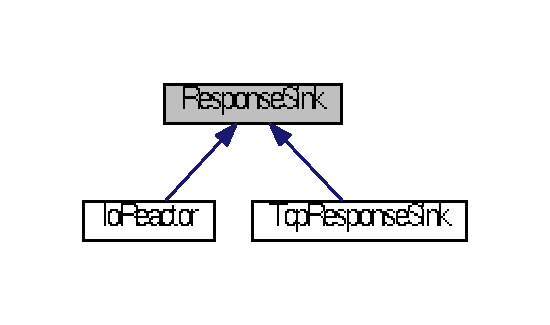
\includegraphics[width=264pt]{classResponseSink__inherit__graph}
\end{center}
\end{figure}
\subsection*{Public Types}
\begin{DoxyCompactItemize}
\item 
\hypertarget{classResponseSink_a4a5be6c1c271b979d28388974ae86ad2}{using \hyperlink{classResponseSink_a4a5be6c1c271b979d28388974ae86ad2}{Callback} = std\+::function$<$ void(\hyperlink{classResponseSink}{Response\+Sink} \&)$>$}\label{classResponseSink_a4a5be6c1c271b979d28388974ae86ad2}

\begin{DoxyCompactList}\small\item\em A type for callbacks taking a \hyperlink{classResponseSink}{Response\+Sink}. \end{DoxyCompactList}\end{DoxyCompactItemize}
\subsection*{Public Member Functions}
\begin{DoxyCompactItemize}
\item 
void \hyperlink{classResponseSink_ac2add6144c2804a6f0db34ad30046ed7}{Respond} (\hyperlink{io__response_8hpp_af5828b68a5f305a17b90321710d9b546}{Response\+Code} code, const std\+::string \&message) const 
\begin{DoxyCompactList}\small\item\em Outputs a response. \end{DoxyCompactList}\item 
void \hyperlink{classResponseSink_a42833a0f1f5e250aa7a41e8bb2fdaac9}{Respond\+With\+Error} (const \hyperlink{classError}{Error} \&error) const 
\begin{DoxyCompactList}\small\item\em Emits an error as a response. \end{DoxyCompactList}\end{DoxyCompactItemize}
\subsection*{Protected Member Functions}
\begin{DoxyCompactItemize}
\item 
virtual void \hyperlink{classResponseSink_a128a514e39f23f2bcc97fea62e9de3c5}{Respond\+Raw} (const std\+::string \&string) const =0
\begin{DoxyCompactList}\small\item\em Outputs a raw response string. \end{DoxyCompactList}\end{DoxyCompactItemize}


\subsection{Detailed Description}
Abstract class for anything that can be sent a response. 

Usually the responses come from a \hyperlink{classResponseSource}{Response\+Source}, but anything may send a \hyperlink{classResponseSink}{Response\+Sink} a response. \begin{DoxySeeAlso}{See also}
\hyperlink{classResponseSource}{Response\+Source} 
\end{DoxySeeAlso}


Definition at line \hyperlink{io__response_8hpp_source_l00049}{49} of file \hyperlink{io__response_8hpp_source}{io\+\_\+response.\+hpp}.



\subsection{Member Function Documentation}
\hypertarget{classResponseSink_ac2add6144c2804a6f0db34ad30046ed7}{\index{Response\+Sink@{Response\+Sink}!Respond@{Respond}}
\index{Respond@{Respond}!Response\+Sink@{Response\+Sink}}
\subsubsection[{Respond}]{\setlength{\rightskip}{0pt plus 5cm}void Response\+Sink\+::\+Respond (
\begin{DoxyParamCaption}
\item[{{\bf Response\+Code}}]{code, }
\item[{const std\+::string \&}]{message}
\end{DoxyParamCaption}
) const}}\label{classResponseSink_ac2add6144c2804a6f0db34ad30046ed7}


Outputs a response. 


\begin{DoxyParams}{Parameters}
{\em code} & The response code to emit. \\
\hline
{\em message} & The response message. \\
\hline
\end{DoxyParams}


Definition at line \hyperlink{io__response_8cpp_source_l00025}{25} of file \hyperlink{io__response_8cpp_source}{io\+\_\+response.\+cpp}.



References \hyperlink{classResponseSink_a128a514e39f23f2bcc97fea62e9de3c5}{Respond\+Raw()}, and \hyperlink{io__response_8cpp_source_l00013}{R\+E\+S\+P\+O\+N\+S\+E\+S}.



Referenced by \hyperlink{player__file_8cpp_source_l00018}{Player\+File\+::\+Emit()}, \hyperlink{player__state_8cpp_source_l00052}{Player\+State\+::\+Emit()}, \hyperlink{tokeniser_8cpp_source_l00113}{Tokeniser\+::\+Emit()}, \hyperlink{player__position_8cpp_source_l00067}{Player\+Position\+::\+Emit()}, \hyperlink{player_8cpp_source_l00045}{Player\+::\+Playback\+Update()}, \hyperlink{io__response_8cpp_source_l00033}{Respond\+With\+Error()}, and \hyperlink{player_8cpp_source_l00058}{Player\+::\+Welcome\+Client()}.


\begin{DoxyCode}
00026 \{
00027     \textcolor{comment}{// ResponseCodes are formatted as "CODE message\(\backslash\)n".}
00028     \textcolor{comment}{// Delegate the actual sending of the response string to the concrete}
00029     \textcolor{comment}{// implementation.}
00030     \hyperlink{classResponseSink_a128a514e39f23f2bcc97fea62e9de3c5}{RespondRaw}(\hyperlink{io__response_8cpp_a9c1b923184d71c13e3dccf3756c20986}{RESPONSES}[static\_cast<int>(code)] + \textcolor{stringliteral}{" "} + message);
00031 \}
\end{DoxyCode}
\hypertarget{classResponseSink_a128a514e39f23f2bcc97fea62e9de3c5}{\index{Response\+Sink@{Response\+Sink}!Respond\+Raw@{Respond\+Raw}}
\index{Respond\+Raw@{Respond\+Raw}!Response\+Sink@{Response\+Sink}}
\subsubsection[{Respond\+Raw}]{\setlength{\rightskip}{0pt plus 5cm}virtual void Response\+Sink\+::\+Respond\+Raw (
\begin{DoxyParamCaption}
\item[{const std\+::string \&}]{string}
\end{DoxyParamCaption}
) const\hspace{0.3cm}{\ttfamily [protected]}, {\ttfamily [pure virtual]}}}\label{classResponseSink_a128a514e39f23f2bcc97fea62e9de3c5}


Outputs a raw response string. 


\begin{DoxyParams}{Parameters}
{\em string} & The response string, of the form \char`\"{}\+C\+O\+D\+E message\char`\"{}. \\
\hline
\end{DoxyParams}


Implemented in \hyperlink{classTcpResponseSink_a20cbf1820d293f620d6ce030fd5aadc6}{Tcp\+Response\+Sink}, and \hyperlink{classIoReactor_a4cfe12db93bda3f7b2c29436c4969006}{Io\+Reactor}.



Referenced by \hyperlink{io__response_8cpp_source_l00025}{Respond()}.

\hypertarget{classResponseSink_a42833a0f1f5e250aa7a41e8bb2fdaac9}{\index{Response\+Sink@{Response\+Sink}!Respond\+With\+Error@{Respond\+With\+Error}}
\index{Respond\+With\+Error@{Respond\+With\+Error}!Response\+Sink@{Response\+Sink}}
\subsubsection[{Respond\+With\+Error}]{\setlength{\rightskip}{0pt plus 5cm}void Response\+Sink\+::\+Respond\+With\+Error (
\begin{DoxyParamCaption}
\item[{const {\bf Error} \&}]{error}
\end{DoxyParamCaption}
) const}}\label{classResponseSink_a42833a0f1f5e250aa7a41e8bb2fdaac9}


Emits an error as a response. 


\begin{DoxyParams}{Parameters}
{\em error} & The error to convert to a response. \\
\hline
\end{DoxyParams}


Definition at line \hyperlink{io__response_8cpp_source_l00033}{33} of file \hyperlink{io__response_8cpp_source}{io\+\_\+response.\+cpp}.



References \hyperlink{io__response_8hpp_af5828b68a5f305a17b90321710d9b546ac2759effffc94bb9acc71d69fe3e8a1f}{F\+A\+I\+L}, \hyperlink{errors_8cpp_source_l00017}{Error\+::\+Message()}, and \hyperlink{io__response_8cpp_source_l00025}{Respond()}.


\begin{DoxyCode}
00034 \{
00035     \hyperlink{classResponseSink_ac2add6144c2804a6f0db34ad30046ed7}{Respond}(\hyperlink{io__response_8hpp_af5828b68a5f305a17b90321710d9b546ac2759effffc94bb9acc71d69fe3e8a1f}{ResponseCode::FAIL}, error.\hyperlink{classError_a006605b13a346cf019f60420f1b29b5a}{Message}());
00036 \}
\end{DoxyCode}


The documentation for this class was generated from the following files\+:\begin{DoxyCompactItemize}
\item 
src/io/\hyperlink{io__response_8hpp}{io\+\_\+response.\+hpp}\item 
src/io/\hyperlink{io__response_8cpp}{io\+\_\+response.\+cpp}\end{DoxyCompactItemize}

\hypertarget{classResponseSource}{\section{Response\+Source Class Reference}
\label{classResponseSource}\index{Response\+Source@{Response\+Source}}
}


Abstract helper class for sources of responses.  




{\ttfamily \#include $<$io\+\_\+response.\+hpp$>$}



Inheritance diagram for Response\+Source\+:
\nopagebreak
\begin{figure}[H]
\begin{center}
\leavevmode
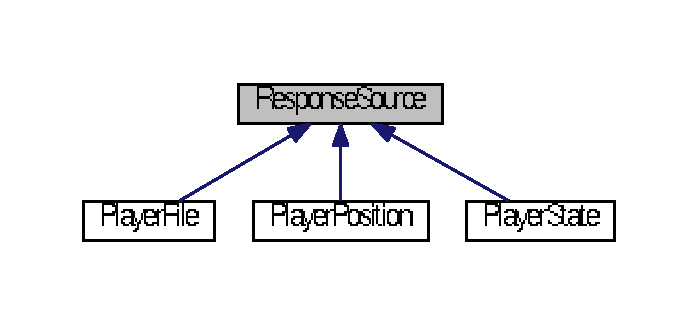
\includegraphics[width=335pt]{classResponseSource__inherit__graph}
\end{center}
\end{figure}


Collaboration diagram for Response\+Source\+:
\nopagebreak
\begin{figure}[H]
\begin{center}
\leavevmode
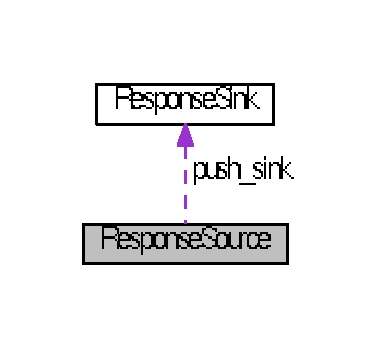
\includegraphics[width=180pt]{classResponseSource__coll__graph}
\end{center}
\end{figure}
\subsection*{Public Member Functions}
\begin{DoxyCompactItemize}
\item 
virtual void \hyperlink{classResponseSource_a498ee53cca912cdb6d48043108c39dc1}{Emit} (\hyperlink{classResponseSink}{Response\+Sink} \&sink) const =0
\begin{DoxyCompactList}\small\item\em Emits a response to a given \hyperlink{classResponseSink}{Response\+Sink}. \end{DoxyCompactList}\item 
void \hyperlink{classResponseSource_a12c45136716adffa59d5e5e1ca80b7ce}{Set\+Response\+Sink} (\hyperlink{classResponseSink}{Response\+Sink} \&sink)
\begin{DoxyCompactList}\small\item\em Registers a \hyperlink{classResponseSink}{Response\+Sink} with this \hyperlink{classResponseSource}{Response\+Source}. \end{DoxyCompactList}\end{DoxyCompactItemize}
\subsection*{Protected Member Functions}
\begin{DoxyCompactItemize}
\item 
void \hyperlink{classResponseSource_a6e3b93326ee043f6d60510acd08de69b}{Push} () const 
\begin{DoxyCompactList}\small\item\em Calls an Emit on the registered \hyperlink{classResponseSink}{Response\+Sink}. \end{DoxyCompactList}\end{DoxyCompactItemize}
\subsection*{Private Attributes}
\begin{DoxyCompactItemize}
\item 
\hyperlink{classResponseSink}{Response\+Sink} $\ast$ \hyperlink{classResponseSource_a8a3ce306db2d1a0a9b9c563e5e8c4b31}{push\+\_\+sink}
\begin{DoxyCompactList}\small\item\em A \hyperlink{classResponseSink}{Response\+Sink} to which 'push' responses are emitted. \end{DoxyCompactList}\end{DoxyCompactItemize}


\subsection{Detailed Description}
Abstract helper class for sources of responses. 

A \hyperlink{classResponseSource}{Response\+Source} can both 'push' responses to a registered \hyperlink{classResponseSink}{Response\+Sink} and be 'polled' from outside to dump its current response to an external \hyperlink{classResponseSink}{Response\+Sink}. For example, \hyperlink{classPlayerPosition}{Player\+Position} 'pushes' its position every few milliseconds to the outside world, to keep the client aware of the time, but is also 'polled' on a new client connection so that the client immediately gets the current position on connect.

\begin{DoxySeeAlso}{See also}
\hyperlink{classResponseSink}{Response\+Sink} 
\end{DoxySeeAlso}


Definition at line \hyperlink{io__response_8hpp_source_l00087}{87} of file \hyperlink{io__response_8hpp_source}{io\+\_\+response.\+hpp}.



\subsection{Member Function Documentation}
\hypertarget{classResponseSource_a498ee53cca912cdb6d48043108c39dc1}{\index{Response\+Source@{Response\+Source}!Emit@{Emit}}
\index{Emit@{Emit}!Response\+Source@{Response\+Source}}
\subsubsection[{Emit}]{\setlength{\rightskip}{0pt plus 5cm}virtual void Response\+Source\+::\+Emit (
\begin{DoxyParamCaption}
\item[{{\bf Response\+Sink} \&}]{sink}
\end{DoxyParamCaption}
) const\hspace{0.3cm}{\ttfamily [pure virtual]}}}\label{classResponseSource_a498ee53cca912cdb6d48043108c39dc1}


Emits a response to a given \hyperlink{classResponseSink}{Response\+Sink}. 


\begin{DoxyParams}{Parameters}
{\em sink} & The \hyperlink{classResponseSink}{Response\+Sink} to which this \hyperlink{classResponseSource}{Response\+Source}'s current response should be emitted. \\
\hline
\end{DoxyParams}


Implemented in \hyperlink{classPlayerPosition_a66963c28fd9dffe0fd7338023310fa92}{Player\+Position}, \hyperlink{classPlayerState_aa93a9879688bfbd3d89ac102c079cbfd}{Player\+State}, and \hyperlink{classPlayerFile_a00f044c74d07d778532953a917c24197}{Player\+File}.



Referenced by \hyperlink{io__response_8cpp_source_l00047}{Push()}.

\hypertarget{classResponseSource_a6e3b93326ee043f6d60510acd08de69b}{\index{Response\+Source@{Response\+Source}!Push@{Push}}
\index{Push@{Push}!Response\+Source@{Response\+Source}}
\subsubsection[{Push}]{\setlength{\rightskip}{0pt plus 5cm}void Response\+Source\+::\+Push (
\begin{DoxyParamCaption}
{}
\end{DoxyParamCaption}
) const\hspace{0.3cm}{\ttfamily [protected]}}}\label{classResponseSource_a6e3b93326ee043f6d60510acd08de69b}


Calls an Emit on the registered \hyperlink{classResponseSink}{Response\+Sink}. 

If there is no registered \hyperlink{classResponseSink}{Response\+Sink}, the response is dropped. 

Definition at line \hyperlink{io__response_8cpp_source_l00047}{47} of file \hyperlink{io__response_8cpp_source}{io\+\_\+response.\+cpp}.



References \hyperlink{classResponseSource_a498ee53cca912cdb6d48043108c39dc1}{Emit()}, and \hyperlink{io__response_8hpp_source_l00116}{push\+\_\+sink}.



Referenced by \hyperlink{player__state_8cpp_source_l00079}{Player\+State\+::\+Set()}, and \hyperlink{player__position_8cpp_source_l00049}{Player\+Position\+::\+Update()}.


\begin{DoxyCode}
00048 \{
00049     \textcolor{keywordflow}{if} (this->\hyperlink{classResponseSource_a8a3ce306db2d1a0a9b9c563e5e8c4b31}{push\_sink} != \textcolor{keyword}{nullptr}) \{
00050         \hyperlink{classResponseSource_a498ee53cca912cdb6d48043108c39dc1}{Emit}(*this->\hyperlink{classResponseSource_a8a3ce306db2d1a0a9b9c563e5e8c4b31}{push\_sink});
00051     \}
00052 \}
\end{DoxyCode}
\hypertarget{classResponseSource_a12c45136716adffa59d5e5e1ca80b7ce}{\index{Response\+Source@{Response\+Source}!Set\+Response\+Sink@{Set\+Response\+Sink}}
\index{Set\+Response\+Sink@{Set\+Response\+Sink}!Response\+Source@{Response\+Source}}
\subsubsection[{Set\+Response\+Sink}]{\setlength{\rightskip}{0pt plus 5cm}void Response\+Source\+::\+Set\+Response\+Sink (
\begin{DoxyParamCaption}
\item[{{\bf Response\+Sink} \&}]{sink}
\end{DoxyParamCaption}
)}}\label{classResponseSource_a12c45136716adffa59d5e5e1ca80b7ce}


Registers a \hyperlink{classResponseSink}{Response\+Sink} with this \hyperlink{classResponseSource}{Response\+Source}. 

The \hyperlink{classResponseSource}{Response\+Source} will periodically send a response to the given \hyperlink{classResponseSink}{Response\+Sink}. 
\begin{DoxyParams}{Parameters}
{\em sink} & The \hyperlink{classResponseSink}{Response\+Sink} to register. \\
\hline
\end{DoxyParams}


Definition at line \hyperlink{io__response_8cpp_source_l00042}{42} of file \hyperlink{io__response_8cpp_source}{io\+\_\+response.\+cpp}.



References \hyperlink{io__response_8hpp_source_l00116}{push\+\_\+sink}.



Referenced by \hyperlink{player_8cpp_source_l00067}{Player\+::\+Set\+Response\+Sink()}.


\begin{DoxyCode}
00043 \{
00044     this->\hyperlink{classResponseSource_a8a3ce306db2d1a0a9b9c563e5e8c4b31}{push\_sink} = &responder;
00045 \}
\end{DoxyCode}


\subsection{Member Data Documentation}
\hypertarget{classResponseSource_a8a3ce306db2d1a0a9b9c563e5e8c4b31}{\index{Response\+Source@{Response\+Source}!push\+\_\+sink@{push\+\_\+sink}}
\index{push\+\_\+sink@{push\+\_\+sink}!Response\+Source@{Response\+Source}}
\subsubsection[{push\+\_\+sink}]{\setlength{\rightskip}{0pt plus 5cm}{\bf Response\+Sink}$\ast$ Response\+Source\+::push\+\_\+sink\hspace{0.3cm}{\ttfamily [private]}}}\label{classResponseSource_a8a3ce306db2d1a0a9b9c563e5e8c4b31}


A \hyperlink{classResponseSink}{Response\+Sink} to which 'push' responses are emitted. 

If the \hyperlink{classResponseSink}{Response\+Sink} is not present, responses are not emitted. 

Definition at line \hyperlink{io__response_8hpp_source_l00116}{116} of file \hyperlink{io__response_8hpp_source}{io\+\_\+response.\+hpp}.



Referenced by \hyperlink{io__response_8cpp_source_l00047}{Push()}, and \hyperlink{io__response_8cpp_source_l00042}{Set\+Response\+Sink()}.



The documentation for this class was generated from the following files\+:\begin{DoxyCompactItemize}
\item 
src/io/\hyperlink{io__response_8hpp}{io\+\_\+response.\+hpp}\item 
src/io/\hyperlink{io__response_8cpp}{io\+\_\+response.\+cpp}\end{DoxyCompactItemize}

\hypertarget{classRingBuffer}{\section{Ring\+Buffer$<$ Rep\+T, Sample\+Count\+T $>$ Class Template Reference}
\label{classRingBuffer}\index{Ring\+Buffer$<$ Rep\+T, Sample\+Count\+T $>$@{Ring\+Buffer$<$ Rep\+T, Sample\+Count\+T $>$}}
}


A ring buffer.  




{\ttfamily \#include $<$ringbuffer.\+hpp$>$}

\subsection*{Public Member Functions}
\begin{DoxyCompactItemize}
\item 
\hyperlink{classRingBuffer_a2f831ec4941885db960a833cb807465e}{Ring\+Buffer} (int power, int size)
\begin{DoxyCompactList}\small\item\em Constructs a \hyperlink{classRingBuffer}{Ring\+Buffer}. \end{DoxyCompactList}\item 
\hypertarget{classRingBuffer_a39d93b7f608eb69a7a569e61b5abc979}{\hyperlink{classRingBuffer_a39d93b7f608eb69a7a569e61b5abc979}{$\sim$\+Ring\+Buffer} ()}\label{classRingBuffer_a39d93b7f608eb69a7a569e61b5abc979}

\begin{DoxyCompactList}\small\item\em Destructs a Pa\+Ring\+Buffer. \end{DoxyCompactList}\item 
\hypertarget{classRingBuffer_a16e7e006ded5d4aad8b37ee7bea8f90d}{\hyperlink{classRingBuffer_a16e7e006ded5d4aad8b37ee7bea8f90d}{Ring\+Buffer} (const \hyperlink{classRingBuffer}{Ring\+Buffer} \&)=delete}\label{classRingBuffer_a16e7e006ded5d4aad8b37ee7bea8f90d}

\begin{DoxyCompactList}\small\item\em Deleted copy constructor. \end{DoxyCompactList}\item 
\hypertarget{classRingBuffer_a6f552e291e577aeffc57b846969d11d6}{\hyperlink{classRingBuffer}{Ring\+Buffer} \& \hyperlink{classRingBuffer_a6f552e291e577aeffc57b846969d11d6}{operator=} (const \hyperlink{classRingBuffer}{Ring\+Buffer} \&)=delete}\label{classRingBuffer_a6f552e291e577aeffc57b846969d11d6}

\begin{DoxyCompactList}\small\item\em Deleted copy-\/assignment. \end{DoxyCompactList}\item 
Sample\+Count\+T \hyperlink{classRingBuffer_ab00617ab6e379ad146cb7b80079f4c4c}{Write\+Capacity} () const 
\begin{DoxyCompactList}\small\item\em The current write capacity. \end{DoxyCompactList}\item 
Sample\+Count\+T \hyperlink{classRingBuffer_a7086cc66306105db205842af7a88c2d8}{Read\+Capacity} () const 
\begin{DoxyCompactList}\small\item\em The current read capacity. \end{DoxyCompactList}\item 
Sample\+Count\+T \hyperlink{classRingBuffer_aa7f863968cb641946b0cf341bda11e16}{Write} (Rep\+T $\ast$start, Sample\+Count\+T count)
\begin{DoxyCompactList}\small\item\em Writes samples from an array into the ring buffer. \end{DoxyCompactList}\item 
Sample\+Count\+T \hyperlink{classRingBuffer_af892330ee102bd50a493b8afa814a0f0}{Read} (Rep\+T $\ast$start, Sample\+Count\+T count)
\begin{DoxyCompactList}\small\item\em Reads samples from the ring buffer into an array. \end{DoxyCompactList}\item 
\hypertarget{classRingBuffer_a1eb1acca6905e7678fbbdb70238cdc26}{void \hyperlink{classRingBuffer_a1eb1acca6905e7678fbbdb70238cdc26}{Flush} ()}\label{classRingBuffer_a1eb1acca6905e7678fbbdb70238cdc26}

\begin{DoxyCompactList}\small\item\em Empties the ring buffer. \end{DoxyCompactList}\end{DoxyCompactItemize}
\subsection*{Private Member Functions}
\begin{DoxyCompactItemize}
\item 
Sample\+Count\+T \hyperlink{classRingBuffer_ae907c82ba714a087d9f35b089f9fbf77}{Count\+Cast} (ring\+\_\+buffer\+\_\+size\+\_\+t count) const 
\begin{DoxyCompactList}\small\item\em Converts a ring buffer size into an external size. \end{DoxyCompactList}\end{DoxyCompactItemize}
\subsection*{Private Attributes}
\begin{DoxyCompactItemize}
\item 
\hypertarget{classRingBuffer_a09103853af3302b27d2bbd46f1dfbe87}{char $\ast$ \hyperlink{classRingBuffer_a09103853af3302b27d2bbd46f1dfbe87}{buffer}}\label{classRingBuffer_a09103853af3302b27d2bbd46f1dfbe87}

\begin{DoxyCompactList}\small\item\em The array used by the ringbuffer. \end{DoxyCompactList}\item 
\hypertarget{classRingBuffer_a10985ec171bcc15c1301dc74fcb6e7b2}{Pa\+Util\+Ring\+Buffer $\ast$ \hyperlink{classRingBuffer_a10985ec171bcc15c1301dc74fcb6e7b2}{rb}}\label{classRingBuffer_a10985ec171bcc15c1301dc74fcb6e7b2}

\begin{DoxyCompactList}\small\item\em The internal Port\+Audio ringbuffer. \end{DoxyCompactList}\end{DoxyCompactItemize}


\subsection{Detailed Description}
\subsubsection*{template$<$typename Rep\+T, typename Sample\+Count\+T$>$class Ring\+Buffer$<$ Rep\+T, Sample\+Count\+T $>$}

A ring buffer. 

This ring buffer is based on the Port\+Audio ring buffer, provided in the contrib/ directory. This is stable and performs well, but, as it is C code, necessitates some hoop jumping to integrate and could do with being replaced with a native solution. 

Definition at line \hyperlink{ringbuffer_8hpp_source_l00030}{30} of file \hyperlink{ringbuffer_8hpp_source}{ringbuffer.\+hpp}.



\subsection{Constructor \& Destructor Documentation}
\hypertarget{classRingBuffer_a2f831ec4941885db960a833cb807465e}{\index{Ring\+Buffer@{Ring\+Buffer}!Ring\+Buffer@{Ring\+Buffer}}
\index{Ring\+Buffer@{Ring\+Buffer}!Ring\+Buffer@{Ring\+Buffer}}
\subsubsection[{Ring\+Buffer}]{\setlength{\rightskip}{0pt plus 5cm}template$<$typename Rep\+T, typename Sample\+Count\+T$>$ {\bf Ring\+Buffer}$<$ Rep\+T, Sample\+Count\+T $>$\+::{\bf Ring\+Buffer} (
\begin{DoxyParamCaption}
\item[{int}]{power, }
\item[{int}]{size}
\end{DoxyParamCaption}
)\hspace{0.3cm}{\ttfamily [inline]}}}\label{classRingBuffer_a2f831ec4941885db960a833cb807465e}


Constructs a \hyperlink{classRingBuffer}{Ring\+Buffer}. 


\begin{DoxyItemize}
\item Precondition\+: 0 $<$ power, 0 $<$ size.
\item Postcondition\+: The \hyperlink{classRingBuffer}{Ring\+Buffer} is fully initialised.
\end{DoxyItemize}


\begin{DoxyParams}{Parameters}
{\em power} & n, where 2$^\wedge$n is the number of elements in the ring buffer. \\
\hline
{\em size} & The size of one element in the ring buffer. \\
\hline
\end{DoxyParams}


Definition at line \hyperlink{ringbuffer_8hpp_source_l00042}{42} of file \hyperlink{ringbuffer_8hpp_source}{ringbuffer.\+hpp}.


\begin{DoxyCode}
00043     \{
00044         assert(0 < power);
00045         assert(0 < size);
00046 
00047         this->\hyperlink{classRingBuffer_a10985ec171bcc15c1301dc74fcb6e7b2}{rb} = \textcolor{keyword}{new} PaUtilRingBuffer;
00048         this->\hyperlink{classRingBuffer_a09103853af3302b27d2bbd46f1dfbe87}{buffer} = \textcolor{keyword}{new} \textcolor{keywordtype}{char}[(1 << power) * size];
00049 
00050         \textcolor{keywordtype}{int} init\_result = PaUtil\_InitializeRingBuffer(
00051                         this->\hyperlink{classRingBuffer_a10985ec171bcc15c1301dc74fcb6e7b2}{rb}, size,
00052                         static\_cast<ring\_buffer\_size\_t>(1 << power),
00053                         this->\hyperlink{classRingBuffer_a09103853af3302b27d2bbd46f1dfbe87}{buffer});
00054         \textcolor{keywordflow}{if} (init\_result != 0) \{
00055             \textcolor{keywordflow}{throw} \textcolor{keyword}{new} \hyperlink{classInternalError}{InternalError}(\hyperlink{messages_8h_a3bf0477dded19418d7ecac95aeae8856}{MSG\_OUTPUT\_RINGINIT});
00056         \}
00057 
00058         assert(this->\hyperlink{classRingBuffer_a10985ec171bcc15c1301dc74fcb6e7b2}{rb} != \textcolor{keyword}{nullptr});
00059         assert(this->\hyperlink{classRingBuffer_a09103853af3302b27d2bbd46f1dfbe87}{buffer} != \textcolor{keyword}{nullptr});
00060     \}
\end{DoxyCode}


\subsection{Member Function Documentation}
\hypertarget{classRingBuffer_ae907c82ba714a087d9f35b089f9fbf77}{\index{Ring\+Buffer@{Ring\+Buffer}!Count\+Cast@{Count\+Cast}}
\index{Count\+Cast@{Count\+Cast}!Ring\+Buffer@{Ring\+Buffer}}
\subsubsection[{Count\+Cast}]{\setlength{\rightskip}{0pt plus 5cm}template$<$typename Rep\+T, typename Sample\+Count\+T$>$ Sample\+Count\+T {\bf Ring\+Buffer}$<$ Rep\+T, Sample\+Count\+T $>$\+::Count\+Cast (
\begin{DoxyParamCaption}
\item[{ring\+\_\+buffer\+\_\+size\+\_\+t}]{count}
\end{DoxyParamCaption}
) const\hspace{0.3cm}{\ttfamily [inline]}, {\ttfamily [private]}}}\label{classRingBuffer_ae907c82ba714a087d9f35b089f9fbf77}


Converts a ring buffer size into an external size. 


\begin{DoxyParams}{Parameters}
{\em count} & The size/count in Port\+Audio form. \\
\hline
\end{DoxyParams}
\begin{DoxyReturn}{Returns}
The size/count after casting to Sample\+Count\+T. 
\end{DoxyReturn}


Definition at line \hyperlink{ringbuffer_8hpp_source_l00174}{174} of file \hyperlink{ringbuffer_8hpp_source}{ringbuffer.\+hpp}.



Referenced by \hyperlink{ringbuffer_8hpp_source_l00149}{Ring\+Buffer$<$ char, unsigned long $>$\+::\+Read()}, \hyperlink{ringbuffer_8hpp_source_l00093}{Ring\+Buffer$<$ char, unsigned long $>$\+::\+Read\+Capacity()}, \hyperlink{ringbuffer_8hpp_source_l00120}{Ring\+Buffer$<$ char, unsigned long $>$\+::\+Write()}, and \hyperlink{ringbuffer_8hpp_source_l00083}{Ring\+Buffer$<$ char, unsigned long $>$\+::\+Write\+Capacity()}.


\begin{DoxyCode}
00175     \{
00176         \textcolor{keywordflow}{return} \textcolor{keyword}{static\_cast<}SampleCountT\textcolor{keyword}{>}(count);
00177     \}
\end{DoxyCode}
\hypertarget{classRingBuffer_af892330ee102bd50a493b8afa814a0f0}{\index{Ring\+Buffer@{Ring\+Buffer}!Read@{Read}}
\index{Read@{Read}!Ring\+Buffer@{Ring\+Buffer}}
\subsubsection[{Read}]{\setlength{\rightskip}{0pt plus 5cm}template$<$typename Rep\+T, typename Sample\+Count\+T$>$ Sample\+Count\+T {\bf Ring\+Buffer}$<$ Rep\+T, Sample\+Count\+T $>$\+::Read (
\begin{DoxyParamCaption}
\item[{Rep\+T $\ast$}]{start, }
\item[{Sample\+Count\+T}]{count}
\end{DoxyParamCaption}
)\hspace{0.3cm}{\ttfamily [inline]}}}\label{classRingBuffer_af892330ee102bd50a493b8afa814a0f0}


Reads samples from the ring buffer into an array. 

To read one sample, pass a count of 1 and take a pointer to the sample variable.


\begin{DoxyItemize}
\item Precondition\+: start points to a valid array, 0 $<$ count $<$= the size of the block of memory pointed to by start, count $<$= \hyperlink{classRingBuffer_a7086cc66306105db205842af7a88c2d8}{Read\+Capacity()}.
\item Postcondition\+: The block of memory pointed to by start and bounded by count and \hyperlink{classRingBuffer_a7086cc66306105db205842af7a88c2d8}{Read\+Capacity()} has been filled with the appropriate number of samples from the front of the ring buffer.
\end{DoxyItemize}


\begin{DoxyParams}{Parameters}
{\em start} & The start of the array buffer to which we write samples. Must not be nullptr. \\
\hline
{\em count} & The number of samples to read. This must not exceed the minimum of \hyperlink{classRingBuffer_a7086cc66306105db205842af7a88c2d8}{Read\+Capacity()} and the length of the array. \\
\hline
\end{DoxyParams}
\begin{DoxyReturn}{Returns}
The number of samples read, which should not exceed count. 
\end{DoxyReturn}
\begin{DoxySeeAlso}{See also}
\hyperlink{classRingBuffer_a7086cc66306105db205842af7a88c2d8}{Read\+Capacity} 
\end{DoxySeeAlso}


Definition at line \hyperlink{ringbuffer_8hpp_source_l00149}{149} of file \hyperlink{ringbuffer_8hpp_source}{ringbuffer.\+hpp}.



Referenced by \hyperlink{audio__sink_8cpp_source_l00176}{Audio\+Sink\+::\+Read\+Samples\+To\+Output()}.


\begin{DoxyCode}
00150     \{
00151         assert(0 < count);
00152         assert(count <= \hyperlink{classRingBuffer_a7086cc66306105db205842af7a88c2d8}{ReadCapacity}());
00153 
00154         \textcolor{keywordflow}{return} \hyperlink{classRingBuffer_ae907c82ba714a087d9f35b089f9fbf77}{CountCast}(PaUtil\_ReadRingBuffer(
00155                         this->\hyperlink{classRingBuffer_a10985ec171bcc15c1301dc74fcb6e7b2}{rb}, start,
00156                         static\_cast<ring\_buffer\_size\_t>(count)));
00157     \}
\end{DoxyCode}
\hypertarget{classRingBuffer_a7086cc66306105db205842af7a88c2d8}{\index{Ring\+Buffer@{Ring\+Buffer}!Read\+Capacity@{Read\+Capacity}}
\index{Read\+Capacity@{Read\+Capacity}!Ring\+Buffer@{Ring\+Buffer}}
\subsubsection[{Read\+Capacity}]{\setlength{\rightskip}{0pt plus 5cm}template$<$typename Rep\+T, typename Sample\+Count\+T$>$ Sample\+Count\+T {\bf Ring\+Buffer}$<$ Rep\+T, Sample\+Count\+T $>$\+::Read\+Capacity (
\begin{DoxyParamCaption}
{}
\end{DoxyParamCaption}
) const\hspace{0.3cm}{\ttfamily [inline]}}}\label{classRingBuffer_a7086cc66306105db205842af7a88c2d8}


The current read capacity. 

\begin{DoxyReturn}{Returns}
The number of samples available in this ring buffer. 
\end{DoxyReturn}
\begin{DoxySeeAlso}{See also}
\hyperlink{classRingBuffer_af892330ee102bd50a493b8afa814a0f0}{Read} 
\end{DoxySeeAlso}


Definition at line \hyperlink{ringbuffer_8hpp_source_l00093}{93} of file \hyperlink{ringbuffer_8hpp_source}{ringbuffer.\+hpp}.



Referenced by \hyperlink{audio__sink_8cpp_source_l00126}{Audio\+Sink\+::\+Play\+Callback\+Step()}, and \hyperlink{ringbuffer_8hpp_source_l00149}{Ring\+Buffer$<$ char, unsigned long $>$\+::\+Read()}.


\begin{DoxyCode}
00094     \{
00095         \textcolor{keywordflow}{return} \hyperlink{classRingBuffer_ae907c82ba714a087d9f35b089f9fbf77}{CountCast}(PaUtil\_GetRingBufferReadAvailable(this->\hyperlink{classRingBuffer_a10985ec171bcc15c1301dc74fcb6e7b2}{rb}));
00096     \}
\end{DoxyCode}
\hypertarget{classRingBuffer_aa7f863968cb641946b0cf341bda11e16}{\index{Ring\+Buffer@{Ring\+Buffer}!Write@{Write}}
\index{Write@{Write}!Ring\+Buffer@{Ring\+Buffer}}
\subsubsection[{Write}]{\setlength{\rightskip}{0pt plus 5cm}template$<$typename Rep\+T, typename Sample\+Count\+T$>$ Sample\+Count\+T {\bf Ring\+Buffer}$<$ Rep\+T, Sample\+Count\+T $>$\+::Write (
\begin{DoxyParamCaption}
\item[{Rep\+T $\ast$}]{start, }
\item[{Sample\+Count\+T}]{count}
\end{DoxyParamCaption}
)\hspace{0.3cm}{\ttfamily [inline]}}}\label{classRingBuffer_aa7f863968cb641946b0cf341bda11e16}


Writes samples from an array into the ring buffer. 

To write one sample, pass a count of 1 and take a pointer to the sample variable. Note that start pointer is not constant. This is because the underlying implementation of the ring buffer might not guarantee that the array is left untouched.


\begin{DoxyItemize}
\item Precondition\+: start points to a valid array, 0 $<$ count $<$= the size of the block of memory pointed to by start, count $<$= \hyperlink{classRingBuffer_ab00617ab6e379ad146cb7b80079f4c4c}{Write\+Capacity()}.
\item Postcondition\+: The ringbuffer has been written to with the contents of the memory pointed to by start and bounded by count and \hyperlink{classRingBuffer_ab00617ab6e379ad146cb7b80079f4c4c}{Write\+Capacity()}.
\end{DoxyItemize}


\begin{DoxyParams}{Parameters}
{\em start} & The start of the array buffer from which we read samples. Must not be nullptr. \\
\hline
{\em count} & The number of samples to write. This must not exceed the minimum of \hyperlink{classRingBuffer_ab00617ab6e379ad146cb7b80079f4c4c}{Write\+Capacity()} and the length of the array. \\
\hline
\end{DoxyParams}
\begin{DoxyReturn}{Returns}
The number of samples written, which should not exceed count. 
\end{DoxyReturn}
\begin{DoxySeeAlso}{See also}
\hyperlink{classRingBuffer_ab00617ab6e379ad146cb7b80079f4c4c}{Write\+Capacity} 
\end{DoxySeeAlso}


Definition at line \hyperlink{ringbuffer_8hpp_source_l00120}{120} of file \hyperlink{ringbuffer_8hpp_source}{ringbuffer.\+hpp}.



Referenced by \hyperlink{audio__sink_8cpp_source_l00076}{Audio\+Sink\+::\+Transfer()}.


\begin{DoxyCode}
00121     \{
00122         assert(0 < count);
00123         assert(count <= \hyperlink{classRingBuffer_ab00617ab6e379ad146cb7b80079f4c4c}{WriteCapacity}());
00124 
00125         \textcolor{keywordflow}{return} \hyperlink{classRingBuffer_ae907c82ba714a087d9f35b089f9fbf77}{CountCast}(PaUtil\_WriteRingBuffer(
00126                         this->\hyperlink{classRingBuffer_a10985ec171bcc15c1301dc74fcb6e7b2}{rb}, start,
00127                         static\_cast<ring\_buffer\_size\_t>(count)));
00128     \}
\end{DoxyCode}
\hypertarget{classRingBuffer_ab00617ab6e379ad146cb7b80079f4c4c}{\index{Ring\+Buffer@{Ring\+Buffer}!Write\+Capacity@{Write\+Capacity}}
\index{Write\+Capacity@{Write\+Capacity}!Ring\+Buffer@{Ring\+Buffer}}
\subsubsection[{Write\+Capacity}]{\setlength{\rightskip}{0pt plus 5cm}template$<$typename Rep\+T, typename Sample\+Count\+T$>$ Sample\+Count\+T {\bf Ring\+Buffer}$<$ Rep\+T, Sample\+Count\+T $>$\+::Write\+Capacity (
\begin{DoxyParamCaption}
{}
\end{DoxyParamCaption}
) const\hspace{0.3cm}{\ttfamily [inline]}}}\label{classRingBuffer_ab00617ab6e379ad146cb7b80079f4c4c}


The current write capacity. 

\begin{DoxyReturn}{Returns}
The number of samples this ring buffer has space to store. 
\end{DoxyReturn}
\begin{DoxySeeAlso}{See also}
\hyperlink{classRingBuffer_aa7f863968cb641946b0cf341bda11e16}{Write} 
\end{DoxySeeAlso}


Definition at line \hyperlink{ringbuffer_8hpp_source_l00083}{83} of file \hyperlink{ringbuffer_8hpp_source}{ringbuffer.\+hpp}.



Referenced by \hyperlink{audio__sink_8cpp_source_l00076}{Audio\+Sink\+::\+Transfer()}, and \hyperlink{ringbuffer_8hpp_source_l00120}{Ring\+Buffer$<$ char, unsigned long $>$\+::\+Write()}.


\begin{DoxyCode}
00084     \{
00085         \textcolor{keywordflow}{return} \hyperlink{classRingBuffer_ae907c82ba714a087d9f35b089f9fbf77}{CountCast}(PaUtil\_GetRingBufferWriteAvailable(this->\hyperlink{classRingBuffer_a10985ec171bcc15c1301dc74fcb6e7b2}{rb}));
00086     \}
\end{DoxyCode}


The documentation for this class was generated from the following file\+:\begin{DoxyCompactItemize}
\item 
src/audio/\hyperlink{ringbuffer_8hpp}{ringbuffer.\+hpp}\end{DoxyCompactItemize}

\hypertarget{classTcpResponseSink}{\section{Tcp\+Response\+Sink Class Reference}
\label{classTcpResponseSink}\index{Tcp\+Response\+Sink@{Tcp\+Response\+Sink}}
}


A T\+C\+P connection from a client.  




{\ttfamily \#include $<$io\+\_\+reactor.\+hpp$>$}



Inheritance diagram for Tcp\+Response\+Sink\+:
\nopagebreak
\begin{figure}[H]
\begin{center}
\leavevmode
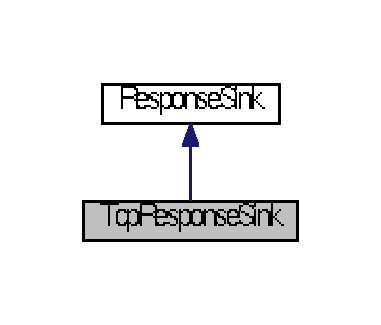
\includegraphics[width=183pt]{classTcpResponseSink__inherit__graph}
\end{center}
\end{figure}


Collaboration diagram for Tcp\+Response\+Sink\+:
\nopagebreak
\begin{figure}[H]
\begin{center}
\leavevmode
\includegraphics[width=350pt]{classTcpResponseSink__coll__graph}
\end{center}
\end{figure}
\subsection*{Public Member Functions}
\begin{DoxyCompactItemize}
\item 
\hyperlink{classTcpResponseSink_aebb4578dd7b9ff9d414c936a27d0969f}{Tcp\+Response\+Sink} (\hyperlink{classIoReactor}{Io\+Reactor} \&\hyperlink{classTcpResponseSink_a190e607290f6ba6b3655c99e44a5e56e}{parent}, uv\+\_\+tcp\+\_\+t $\ast$\hyperlink{classTcpResponseSink_afa43e15736053cef76fbf27bdc3197a9}{tcp}, \hyperlink{classCommandHandler}{Command\+Handler} \&handler)
\begin{DoxyCompactList}\small\item\em Constructs a \hyperlink{classTcpResponseSink}{Tcp\+Response\+Sink}. \end{DoxyCompactList}\item 
void \hyperlink{classTcpResponseSink_a20cbf1820d293f620d6ce030fd5aadc6}{Respond\+Raw} (const std\+::string \&response) const override
\begin{DoxyCompactList}\small\item\em Outputs a raw response string. \end{DoxyCompactList}\item 
void \hyperlink{classTcpResponseSink_a9ee277599dbd6cfc5853a9145f21694b}{Read} (uv\+\_\+stream\+\_\+t $\ast$stream, ssize\+\_\+t nread, const uv\+\_\+buf\+\_\+t $\ast$buf)
\begin{DoxyCompactList}\small\item\em Processes a data read on this connection. \end{DoxyCompactList}\item 
void \hyperlink{classTcpResponseSink_a2e40c526177918ade20bec1e4f66698a}{Close} ()
\begin{DoxyCompactList}\small\item\em Closes this connection. \end{DoxyCompactList}\end{DoxyCompactItemize}
\subsection*{Private Attributes}
\begin{DoxyCompactItemize}
\item 
\hypertarget{classTcpResponseSink_a190e607290f6ba6b3655c99e44a5e56e}{\hyperlink{classIoReactor}{Io\+Reactor} \& \hyperlink{classTcpResponseSink_a190e607290f6ba6b3655c99e44a5e56e}{parent}}\label{classTcpResponseSink_a190e607290f6ba6b3655c99e44a5e56e}

\begin{DoxyCompactList}\small\item\em The parent \hyperlink{classIoReactor}{Io\+Reactor} on which this connection is running. \end{DoxyCompactList}\item 
\hypertarget{classTcpResponseSink_afa43e15736053cef76fbf27bdc3197a9}{uv\+\_\+tcp\+\_\+t $\ast$ \hyperlink{classTcpResponseSink_afa43e15736053cef76fbf27bdc3197a9}{tcp}}\label{classTcpResponseSink_afa43e15736053cef76fbf27bdc3197a9}

\begin{DoxyCompactList}\small\item\em The libuv handle for the T\+C\+P connection. \end{DoxyCompactList}\item 
\hypertarget{classTcpResponseSink_ab289c592752e4c1fdc7d38cc9d6c2aab}{\hyperlink{classTokeniser}{Tokeniser} \hyperlink{classTcpResponseSink_ab289c592752e4c1fdc7d38cc9d6c2aab}{tokeniser}}\label{classTcpResponseSink_ab289c592752e4c1fdc7d38cc9d6c2aab}

\begin{DoxyCompactList}\small\item\em The \hyperlink{classTokeniser}{Tokeniser} to which data read on this connection should be sent. \end{DoxyCompactList}\end{DoxyCompactItemize}
\subsection*{Additional Inherited Members}


\subsection{Detailed Description}
A T\+C\+P connection from a client. 

\begin{DoxyRefDesc}{Todo}
\item[\hyperlink{todo__todo000003}{Todo}]Rename to Connection? \end{DoxyRefDesc}


Definition at line \hyperlink{io__reactor_8hpp_source_l00126}{126} of file \hyperlink{io__reactor_8hpp_source}{io\+\_\+reactor.\+hpp}.



\subsection{Constructor \& Destructor Documentation}
\hypertarget{classTcpResponseSink_aebb4578dd7b9ff9d414c936a27d0969f}{\index{Tcp\+Response\+Sink@{Tcp\+Response\+Sink}!Tcp\+Response\+Sink@{Tcp\+Response\+Sink}}
\index{Tcp\+Response\+Sink@{Tcp\+Response\+Sink}!Tcp\+Response\+Sink@{Tcp\+Response\+Sink}}
\subsubsection[{Tcp\+Response\+Sink}]{\setlength{\rightskip}{0pt plus 5cm}Tcp\+Response\+Sink\+::\+Tcp\+Response\+Sink (
\begin{DoxyParamCaption}
\item[{{\bf Io\+Reactor} \&}]{parent, }
\item[{uv\+\_\+tcp\+\_\+t $\ast$}]{tcp, }
\item[{{\bf Command\+Handler} \&}]{handler}
\end{DoxyParamCaption}
)}}\label{classTcpResponseSink_aebb4578dd7b9ff9d414c936a27d0969f}


Constructs a \hyperlink{classTcpResponseSink}{Tcp\+Response\+Sink}. 


\begin{DoxyParams}{Parameters}
{\em parent} & The \hyperlink{classIoReactor}{Io\+Reactor} that is the parent of this connection. \\
\hline
{\em tcp} & The underlying libuv T\+C\+P stream. \\
\hline
{\em handler} & The handler to which read commands should be sent. \\
\hline
\end{DoxyParams}


Definition at line \hyperlink{io__reactor_8cpp_source_l00192}{192} of file \hyperlink{io__reactor_8cpp_source}{io\+\_\+reactor.\+cpp}.


\begin{DoxyCode}
00194     : \hyperlink{classTcpResponseSink_a190e607290f6ba6b3655c99e44a5e56e}{parent}(parent), \hyperlink{classTcpResponseSink_afa43e15736053cef76fbf27bdc3197a9}{tcp}(\hyperlink{classTcpResponseSink_afa43e15736053cef76fbf27bdc3197a9}{tcp}), \hyperlink{classTcpResponseSink_ab289c592752e4c1fdc7d38cc9d6c2aab}{tokeniser}(handler, *\textcolor{keyword}{this})
00195 \{
00196 \}
\end{DoxyCode}


\subsection{Member Function Documentation}
\hypertarget{classTcpResponseSink_a2e40c526177918ade20bec1e4f66698a}{\index{Tcp\+Response\+Sink@{Tcp\+Response\+Sink}!Close@{Close}}
\index{Close@{Close}!Tcp\+Response\+Sink@{Tcp\+Response\+Sink}}
\subsubsection[{Close}]{\setlength{\rightskip}{0pt plus 5cm}void Tcp\+Response\+Sink\+::\+Close (
\begin{DoxyParamCaption}
{}
\end{DoxyParamCaption}
)}}\label{classTcpResponseSink_a2e40c526177918ade20bec1e4f66698a}


Closes this connection. 

\begin{DoxyRefDesc}{Todo}
\item[\hyperlink{todo__todo000006}{Todo}]Roll into the destructor/use R\+A\+I\+I? \end{DoxyRefDesc}


Definition at line \hyperlink{io__reactor_8cpp_source_l00230}{230} of file \hyperlink{io__reactor_8cpp_source}{io\+\_\+reactor.\+cpp}.



References \hyperlink{io__reactor_8hpp_source_l00158}{parent}, and \hyperlink{io__reactor_8cpp_source_l00133}{Io\+Reactor\+::\+Remove\+Connection()}.



Referenced by \hyperlink{io__reactor_8cpp_source_l00064}{Uv\+Close\+Callback()}.


\begin{DoxyCode}
00231 \{
00232     this->\hyperlink{classTcpResponseSink_a190e607290f6ba6b3655c99e44a5e56e}{parent}.\hyperlink{classIoReactor_af31bb722acf08d10eaa46ea7a1a5d4ca}{RemoveConnection}(*\textcolor{keyword}{this});
00233 \}
\end{DoxyCode}
\hypertarget{classTcpResponseSink_a9ee277599dbd6cfc5853a9145f21694b}{\index{Tcp\+Response\+Sink@{Tcp\+Response\+Sink}!Read@{Read}}
\index{Read@{Read}!Tcp\+Response\+Sink@{Tcp\+Response\+Sink}}
\subsubsection[{Read}]{\setlength{\rightskip}{0pt plus 5cm}void Tcp\+Response\+Sink\+::\+Read (
\begin{DoxyParamCaption}
\item[{uv\+\_\+stream\+\_\+t $\ast$}]{stream, }
\item[{ssize\+\_\+t}]{nread, }
\item[{const uv\+\_\+buf\+\_\+t $\ast$}]{buf}
\end{DoxyParamCaption}
)}}\label{classTcpResponseSink_a9ee277599dbd6cfc5853a9145f21694b}


Processes a data read on this connection. 


\begin{DoxyParams}{Parameters}
{\em stream} & The libuv T\+C\+P/\+I\+P stream providing the data. \\
\hline
{\em nread} & The number of bytes read. \\
\hline
{\em buf} & The buffer containing the read data. \\
\hline
\end{DoxyParams}


Definition at line \hyperlink{io__reactor_8cpp_source_l00213}{213} of file \hyperlink{io__reactor_8cpp_source}{io\+\_\+reactor.\+cpp}.



References \hyperlink{tokeniser_8cpp_source_l00026}{Tokeniser\+::\+Feed()}, \hyperlink{io__reactor_8hpp_source_l00164}{tokeniser}, and \hyperlink{io__reactor_8cpp_source_l00064}{Uv\+Close\+Callback()}.



Referenced by \hyperlink{io__reactor_8cpp_source_l00075}{Uv\+Read\+Callback()}.


\begin{DoxyCode}
00215 \{
00216     \textcolor{keywordflow}{if} (nread < 0) \{
00217         \textcolor{keywordflow}{if} (nread == UV\_EOF) \{
00218             uv\_close((uv\_handle\_t *)stream, \hyperlink{io__reactor_8cpp_ab85791c3e9c737453047decfbb7388f4}{UvCloseCallback});
00219         \}
00220 
00221         \textcolor{keywordflow}{return};
00222     \}
00223 
00224     \textcolor{keywordflow}{if} (buf->base != \textcolor{keyword}{nullptr}) \{
00225         this->\hyperlink{classTcpResponseSink_ab289c592752e4c1fdc7d38cc9d6c2aab}{tokeniser}.\hyperlink{classTokeniser_ab4b8f1238c89d766a1d72f0ee619406d}{Feed}(buf->base, nread);
00226         \textcolor{keyword}{delete}[] buf->base;
00227     \}
00228 \}
\end{DoxyCode}
\hypertarget{classTcpResponseSink_a20cbf1820d293f620d6ce030fd5aadc6}{\index{Tcp\+Response\+Sink@{Tcp\+Response\+Sink}!Respond\+Raw@{Respond\+Raw}}
\index{Respond\+Raw@{Respond\+Raw}!Tcp\+Response\+Sink@{Tcp\+Response\+Sink}}
\subsubsection[{Respond\+Raw}]{\setlength{\rightskip}{0pt plus 5cm}void Tcp\+Response\+Sink\+::\+Respond\+Raw (
\begin{DoxyParamCaption}
\item[{const std\+::string \&}]{string}
\end{DoxyParamCaption}
) const\hspace{0.3cm}{\ttfamily [override]}, {\ttfamily [virtual]}}}\label{classTcpResponseSink_a20cbf1820d293f620d6ce030fd5aadc6}


Outputs a raw response string. 


\begin{DoxyParams}{Parameters}
{\em string} & The response string, of the form \char`\"{}\+C\+O\+D\+E message\char`\"{}. \\
\hline
\end{DoxyParams}


Implements \hyperlink{classResponseSink_a128a514e39f23f2bcc97fea62e9de3c5}{Response\+Sink}.



Definition at line \hyperlink{io__reactor_8cpp_source_l00198}{198} of file \hyperlink{io__reactor_8cpp_source}{io\+\_\+reactor.\+cpp}.



References \hyperlink{io__reactor_8cpp_source_l00054}{Write\+Req\+::buf}, \hyperlink{io__reactor_8hpp_source_l00161}{tcp}, and \hyperlink{io__reactor_8cpp_source_l00092}{Uv\+Respond\+Callback()}.


\begin{DoxyCode}
00199 \{
00200     \hyperlink{classDebug}{Debug}() << \textcolor{stringliteral}{"Sending command:"} << \textcolor{keywordtype}{string} << std::endl;
00201     \textcolor{keywordtype}{unsigned} \textcolor{keywordtype}{int} l = \textcolor{keywordtype}{string}.length();
00202     \textcolor{keyword}{const} \textcolor{keywordtype}{char} *s = \textcolor{keywordtype}{string}.c\_str();
00203 
00204     \hyperlink{structWriteReq}{WriteReq} *req = \textcolor{keyword}{new} \hyperlink{structWriteReq}{WriteReq};
00205     req->\hyperlink{structWriteReq_a2e611e010ab154c56c8055dee140b6b5}{buf} = uv\_buf\_init(\textcolor{keyword}{new} \textcolor{keywordtype}{char}[l + 1], l + 1);
00206     memcpy(req->\hyperlink{structWriteReq_a2e611e010ab154c56c8055dee140b6b5}{buf}.base, s, l);
00207     req->\hyperlink{structWriteReq_a2e611e010ab154c56c8055dee140b6b5}{buf}.base[l] = \textcolor{charliteral}{'\(\backslash\)n'};
00208 
00209     uv\_write((uv\_write\_t *)req, (uv\_stream\_t *)\hyperlink{classTcpResponseSink_afa43e15736053cef76fbf27bdc3197a9}{tcp}, &req->\hyperlink{structWriteReq_a2e611e010ab154c56c8055dee140b6b5}{buf}, 1,
00210              \hyperlink{io__reactor_8cpp_af58ed397c8d93bffdc01b621d4abaa8c}{UvRespondCallback});
00211 \}
\end{DoxyCode}


The documentation for this class was generated from the following files\+:\begin{DoxyCompactItemize}
\item 
src/io/\hyperlink{io__reactor_8hpp}{io\+\_\+reactor.\+hpp}\item 
src/io/\hyperlink{io__reactor_8cpp}{io\+\_\+reactor.\+cpp}\end{DoxyCompactItemize}

\hypertarget{classTimeParser}{\section{Time\+Parser$<$ Out\+Unit, Int\+Type $>$ Class Template Reference}
\label{classTimeParser}\index{Time\+Parser$<$ Out\+Unit, Int\+Type $>$@{Time\+Parser$<$ Out\+Unit, Int\+Type $>$}}
}


A class for parsing time strings consisting of an integer and unit into a flat integer representing the number of Out\+Unit units that time string represents.  




{\ttfamily \#include $<$time\+\_\+parser.\+hpp$>$}

\subsection*{Public Types}
\begin{DoxyCompactItemize}
\item 
\hypertarget{classTimeParser_adc32afc638ace5060a2134f8f74d3c60}{using \hyperlink{classTimeParser_adc32afc638ace5060a2134f8f74d3c60}{Unit\+Map} = std\+::map$<$ std\+::string, std\+::function$<$ Out\+Unit(Int\+Type)$>$$>$}\label{classTimeParser_adc32afc638ace5060a2134f8f74d3c60}

\begin{DoxyCompactList}\small\item\em The type of the map from unit suffixes to functions that convert from an amount of that time unit to a chrono duration of type Out\+Unit capturing the same duration. \end{DoxyCompactList}\end{DoxyCompactItemize}
\subsection*{Public Member Functions}
\begin{DoxyCompactItemize}
\item 
\hyperlink{classTimeParser_a66c6443db8e5d38b8f3d7e7a4eea783a}{Time\+Parser} (const \hyperlink{classTimeParser_adc32afc638ace5060a2134f8f74d3c60}{Unit\+Map} \&\hyperlink{classTimeParser_a98bb2b31f6ad5210139bc87ef7ad0121}{unit\+\_\+map})
\begin{DoxyCompactList}\small\item\em Constructs a \hyperlink{classTimeParser}{Time\+Parser}. \end{DoxyCompactList}\item 
Out\+Unit \hyperlink{classTimeParser_a68110dc8c7d2ad1a8f47a29646ad4d1c}{Parse} (const std\+::string \&time\+\_\+str) const 
\begin{DoxyCompactList}\small\item\em Parses a time, returning it as a std\+::chrono duration. \end{DoxyCompactList}\end{DoxyCompactItemize}
\subsection*{Static Public Member Functions}
\begin{DoxyCompactItemize}
\item 
{\footnotesize template$<$typename In\+Unit $>$ }\\static Out\+Unit \hyperlink{classTimeParser_af0e270392bd5313b1d60e66e35dbfe82}{Mk\+Time} (Int\+Type raw\+\_\+time)
\begin{DoxyCompactList}\small\item\em A template for converting an Int\+Type representation of a duration of In\+Unit units into a duration expressed as an Out\+Unit. \end{DoxyCompactList}\end{DoxyCompactItemize}
\subsection*{Private Member Functions}
\begin{DoxyCompactItemize}
\item 
std\+::pair$<$ std\+::string, Int\+Type $>$ \hyperlink{classTimeParser_a3f7f36a669233d66e7fe1ca8405eefd5}{Split} (const std\+::string \&time\+\_\+str) const 
\begin{DoxyCompactList}\small\item\em Splits a time string into a pair of unit and amount. \end{DoxyCompactList}\end{DoxyCompactItemize}
\subsection*{Private Attributes}
\begin{DoxyCompactItemize}
\item 
\hypertarget{classTimeParser_a98bb2b31f6ad5210139bc87ef7ad0121}{\hyperlink{classTimeParser_adc32afc638ace5060a2134f8f74d3c60}{Unit\+Map} \hyperlink{classTimeParser_a98bb2b31f6ad5210139bc87ef7ad0121}{unit\+\_\+map}}\label{classTimeParser_a98bb2b31f6ad5210139bc87ef7ad0121}

\begin{DoxyCompactList}\small\item\em Map from units to handling functions. \end{DoxyCompactList}\end{DoxyCompactItemize}


\subsection{Detailed Description}
\subsubsection*{template$<$typename Out\+Unit, typename Int\+Type = std\+::uint64\+\_\+t$>$class Time\+Parser$<$ Out\+Unit, Int\+Type $>$}

A class for parsing time strings consisting of an integer and unit into a flat integer representing the number of Out\+Unit units that time string represents. 

Definition at line \hyperlink{time__parser_8hpp_source_l00022}{22} of file \hyperlink{time__parser_8hpp_source}{time\+\_\+parser.\+hpp}.



\subsection{Constructor \& Destructor Documentation}
\hypertarget{classTimeParser_a66c6443db8e5d38b8f3d7e7a4eea783a}{\index{Time\+Parser@{Time\+Parser}!Time\+Parser@{Time\+Parser}}
\index{Time\+Parser@{Time\+Parser}!Time\+Parser@{Time\+Parser}}
\subsubsection[{Time\+Parser}]{\setlength{\rightskip}{0pt plus 5cm}template$<$typename Out\+Unit, typename Int\+Type  = std\+::uint64\+\_\+t$>$ {\bf Time\+Parser}$<$ Out\+Unit, Int\+Type $>$\+::{\bf Time\+Parser} (
\begin{DoxyParamCaption}
\item[{const {\bf Unit\+Map} \&}]{unit\+\_\+map}
\end{DoxyParamCaption}
)\hspace{0.3cm}{\ttfamily [inline]}}}\label{classTimeParser_a66c6443db8e5d38b8f3d7e7a4eea783a}


Constructs a \hyperlink{classTimeParser}{Time\+Parser}. 


\begin{DoxyParams}{Parameters}
{\em unit\+\_\+map} & The map from units to their parsers. \\
\hline
\end{DoxyParams}
\begin{DoxySeeAlso}{See also}
\hyperlink{classTimeParser_af0e270392bd5313b1d60e66e35dbfe82}{Mk\+Time} 
\end{DoxySeeAlso}


Definition at line \hyperlink{time__parser_8hpp_source_l00036}{36} of file \hyperlink{time__parser_8hpp_source}{time\+\_\+parser.\+hpp}.


\begin{DoxyCode}
00036                                         : \hyperlink{classTimeParser_a98bb2b31f6ad5210139bc87ef7ad0121}{unit\_map}(\hyperlink{classTimeParser_a98bb2b31f6ad5210139bc87ef7ad0121}{unit\_map})
00037     \{
00038     \}
\end{DoxyCode}


\subsection{Member Function Documentation}
\hypertarget{classTimeParser_af0e270392bd5313b1d60e66e35dbfe82}{\index{Time\+Parser@{Time\+Parser}!Mk\+Time@{Mk\+Time}}
\index{Mk\+Time@{Mk\+Time}!Time\+Parser@{Time\+Parser}}
\subsubsection[{Mk\+Time}]{\setlength{\rightskip}{0pt plus 5cm}template$<$typename Out\+Unit, typename Int\+Type  = std\+::uint64\+\_\+t$>$ template$<$typename In\+Unit $>$ static Out\+Unit {\bf Time\+Parser}$<$ Out\+Unit, Int\+Type $>$\+::Mk\+Time (
\begin{DoxyParamCaption}
\item[{Int\+Type}]{raw\+\_\+time}
\end{DoxyParamCaption}
)\hspace{0.3cm}{\ttfamily [inline]}, {\ttfamily [static]}}}\label{classTimeParser_af0e270392bd5313b1d60e66e35dbfe82}


A template for converting an Int\+Type representation of a duration of In\+Unit units into a duration expressed as an Out\+Unit. 

For example, \hyperlink{classTimeParser_af0e270392bd5313b1d60e66e35dbfe82}{Mk\+Time$<$std\+::chrono\+::seconds$>$} takes in an Int\+Type of seconds and returns a std\+::chrono\+::microseconds\+: applying this to the integer 1 will result in a microseconds variable representing 1,000,000 microseconds.


\begin{DoxyParams}{Parameters}
{\em raw\+\_\+time} & The raw time, as an integer whose units are those used by In\+Unit. \\
\hline
\end{DoxyParams}
\begin{DoxyReturn}{Returns}
An Out\+Unit capturing the input duration, but in terms of the units used by Out\+Unit. 
\end{DoxyReturn}


Definition at line \hyperlink{time__parser_8hpp_source_l00055}{55} of file \hyperlink{time__parser_8hpp_source}{time\+\_\+parser.\+hpp}.


\begin{DoxyCode}
00056     \{
00057         \textcolor{keywordflow}{return} std::chrono::duration\_cast<OutUnit>(InUnit(raw\_time));
00058     \}
\end{DoxyCode}
\hypertarget{classTimeParser_a68110dc8c7d2ad1a8f47a29646ad4d1c}{\index{Time\+Parser@{Time\+Parser}!Parse@{Parse}}
\index{Parse@{Parse}!Time\+Parser@{Time\+Parser}}
\subsubsection[{Parse}]{\setlength{\rightskip}{0pt plus 5cm}template$<$typename Out\+Unit, typename Int\+Type  = std\+::uint64\+\_\+t$>$ Out\+Unit {\bf Time\+Parser}$<$ Out\+Unit, Int\+Type $>$\+::Parse (
\begin{DoxyParamCaption}
\item[{const std\+::string \&}]{time\+\_\+str}
\end{DoxyParamCaption}
) const\hspace{0.3cm}{\ttfamily [inline]}}}\label{classTimeParser_a68110dc8c7d2ad1a8f47a29646ad4d1c}


Parses a time, returning it as a std\+::chrono duration. 


\begin{DoxyParams}{Parameters}
{\em time\+\_\+str} & The time string. \\
\hline
\end{DoxyParams}
\begin{DoxyReturn}{Returns}
The time, as an instance of Out\+Unit. 
\end{DoxyReturn}


Definition at line \hyperlink{time__parser_8hpp_source_l00065}{65} of file \hyperlink{time__parser_8hpp_source}{time\+\_\+parser.\+hpp}.



Referenced by \hyperlink{player_8cpp_source_l00134}{Player\+::\+Seek()}.


\begin{DoxyCode}
00066     \{
00067         \textcolor{keyword}{auto} seek = \hyperlink{classTimeParser_a3f7f36a669233d66e7fe1ca8405eefd5}{Split}(time\_str);
00068         \textcolor{keywordflow}{return} \hyperlink{classTimeParser_a98bb2b31f6ad5210139bc87ef7ad0121}{unit\_map}.at(seek.first)(seek.second);
00069     \}
\end{DoxyCode}
\hypertarget{classTimeParser_a3f7f36a669233d66e7fe1ca8405eefd5}{\index{Time\+Parser@{Time\+Parser}!Split@{Split}}
\index{Split@{Split}!Time\+Parser@{Time\+Parser}}
\subsubsection[{Split}]{\setlength{\rightskip}{0pt plus 5cm}template$<$typename Out\+Unit, typename Int\+Type  = std\+::uint64\+\_\+t$>$ std\+::pair$<$std\+::string, Int\+Type$>$ {\bf Time\+Parser}$<$ Out\+Unit, Int\+Type $>$\+::Split (
\begin{DoxyParamCaption}
\item[{const std\+::string \&}]{time\+\_\+str}
\end{DoxyParamCaption}
) const\hspace{0.3cm}{\ttfamily [inline]}, {\ttfamily [private]}}}\label{classTimeParser_a3f7f36a669233d66e7fe1ca8405eefd5}


Splits a time string into a pair of unit and amount. 


\begin{DoxyParams}{Parameters}
{\em time\+\_\+str} & The time string. \\
\hline
\end{DoxyParams}
\begin{DoxyReturn}{Returns}
A pair of unit string and time amount, as an integer in terms of the named unit. 
\end{DoxyReturn}


Definition at line \hyperlink{time__parser_8hpp_source_l00080}{80} of file \hyperlink{time__parser_8hpp_source}{time\+\_\+parser.\+hpp}.



Referenced by \hyperlink{time__parser_8hpp_source_l00065}{Time\+Parser$<$ std\+::chrono\+::microseconds $>$\+::\+Parse()}.


\begin{DoxyCode}
00081     \{
00082         std::istringstream is(time\_str);
00083         IntType raw\_time;
00084         std::string rest;
00085 
00086         is >> raw\_time >> rest;
00087         \textcolor{keywordflow}{return} std::make\_pair(rest, raw\_time);
00088     \}
\end{DoxyCode}


The documentation for this class was generated from the following file\+:\begin{DoxyCompactItemize}
\item 
src/\hyperlink{time__parser_8hpp}{time\+\_\+parser.\+hpp}\end{DoxyCompactItemize}

\hypertarget{classTokeniser}{\section{Tokeniser Class Reference}
\label{classTokeniser}\index{Tokeniser@{Tokeniser}}
}


A string tokeniser.  




{\ttfamily \#include $<$tokeniser.\+hpp$>$}



Collaboration diagram for Tokeniser\+:
\nopagebreak
\begin{figure}[H]
\begin{center}
\leavevmode
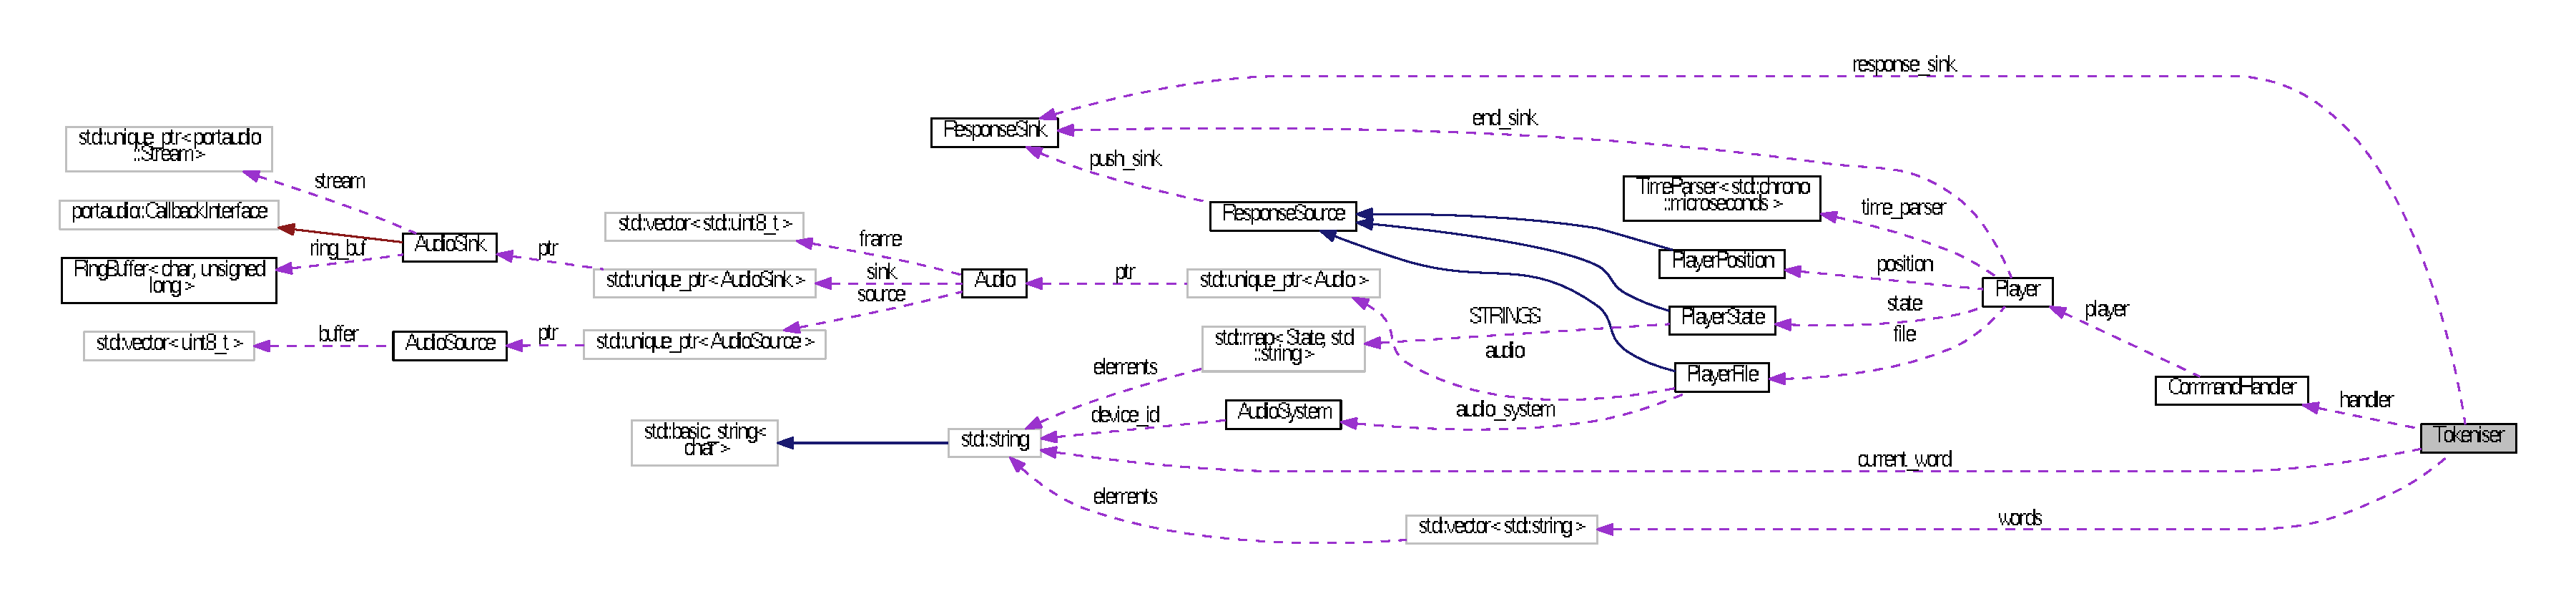
\includegraphics[width=350pt]{classTokeniser__coll__graph}
\end{center}
\end{figure}
\subsection*{Public Member Functions}
\begin{DoxyCompactItemize}
\item 
\hyperlink{classTokeniser_ac69ac105eaf7d81e0632329ee46d2a57}{Tokeniser} (\hyperlink{classCommandHandler}{Command\+Handler} \&\hyperlink{classTokeniser_a779dcc74539e27d10b7d2118fae996e6}{handler}, \hyperlink{classResponseSink}{Response\+Sink} \&\hyperlink{classTokeniser_a5ae6a740655de2f1cbc5f6723dd56439}{response\+\_\+sink})
\begin{DoxyCompactList}\small\item\em Constructs a new \hyperlink{classTokeniser}{Tokeniser}. \end{DoxyCompactList}\item 
void \hyperlink{classTokeniser_ab4b8f1238c89d766a1d72f0ee619406d}{Feed} (const char $\ast$start, unsigned int nread)
\begin{DoxyCompactList}\small\item\em Feeds the contents of a character buffer into a \hyperlink{classTokeniser}{Tokeniser}. \end{DoxyCompactList}\end{DoxyCompactItemize}
\subsection*{Private Types}
\begin{DoxyCompactItemize}
\item 
enum \hyperlink{classTokeniser_a71d622e60fae9d6c36c96ba69a4f62e4}{Quote\+Type} \+: std\+::uint8\+\_\+t \{ \hyperlink{classTokeniser_a71d622e60fae9d6c36c96ba69a4f62e4ab50339a10e1de285ac99d4c3990b8693}{Quote\+Type\+::\+N\+O\+N\+E}, 
\hyperlink{classTokeniser_a71d622e60fae9d6c36c96ba69a4f62e4a0679273e201afd0bf57af3961f8a23b8}{Quote\+Type\+::\+S\+I\+N\+G\+L\+E}, 
\hyperlink{classTokeniser_a71d622e60fae9d6c36c96ba69a4f62e4afd3e4ece78a7d422280d5ed379482229}{Quote\+Type\+::\+D\+O\+U\+B\+L\+E}
 \}
\begin{DoxyCompactList}\small\item\em Enumeration of quotation types. \end{DoxyCompactList}\end{DoxyCompactItemize}
\subsection*{Private Member Functions}
\begin{DoxyCompactItemize}
\item 
\hypertarget{classTokeniser_a71405521b0e9c00a0d9b1a2f32ae10c2}{void \hyperlink{classTokeniser_a71405521b0e9c00a0d9b1a2f32ae10c2}{Emit} ()}\label{classTokeniser_a71405521b0e9c00a0d9b1a2f32ae10c2}

\begin{DoxyCompactList}\small\item\em Finishes the current word and sends the line to the \hyperlink{classCommandHandler}{Command\+Handler}. \end{DoxyCompactList}\item 
\hypertarget{classTokeniser_abb18309e5b6cce8fc63cdb4b02e69bf3}{void \hyperlink{classTokeniser_abb18309e5b6cce8fc63cdb4b02e69bf3}{End\+Word} ()}\label{classTokeniser_abb18309e5b6cce8fc63cdb4b02e69bf3}

\begin{DoxyCompactList}\small\item\em Finishes the current word, adding it to the tokenised line. \end{DoxyCompactList}\item 
void \hyperlink{classTokeniser_a0c62f5dd06a42d478a93595fc78b76fa}{Push} (unsigned char c)
\begin{DoxyCompactList}\small\item\em Pushes a raw character onto the end of the current word. \end{DoxyCompactList}\end{DoxyCompactItemize}
\subsection*{Private Attributes}
\begin{DoxyCompactItemize}
\item 
\hypertarget{classTokeniser_a779dcc74539e27d10b7d2118fae996e6}{\hyperlink{classCommandHandler}{Command\+Handler} \& \hyperlink{classTokeniser_a779dcc74539e27d10b7d2118fae996e6}{handler}}\label{classTokeniser_a779dcc74539e27d10b7d2118fae996e6}

\begin{DoxyCompactList}\small\item\em The command handler to which complete lines should be sent. \end{DoxyCompactList}\item 
\hyperlink{classResponseSink}{Response\+Sink} \& \hyperlink{classTokeniser_a5ae6a740655de2f1cbc5f6723dd56439}{response\+\_\+sink}
\begin{DoxyCompactList}\small\item\em The response sink to which command acknowledgements should be sent. \end{DoxyCompactList}\item 
bool \hyperlink{classTokeniser_ace181afc0f1425b87126becc79458edd}{escape\+\_\+next\+\_\+character}
\begin{DoxyCompactList}\small\item\em Whether the next character is to be interpreted as an escape code. \end{DoxyCompactList}\item 
\hypertarget{classTokeniser_a10b7147e055edd438fcb951fc41faf65}{\hyperlink{classTokeniser_a71d622e60fae9d6c36c96ba69a4f62e4}{Quote\+Type} \hyperlink{classTokeniser_a10b7147e055edd438fcb951fc41faf65}{quote\+\_\+type}}\label{classTokeniser_a10b7147e055edd438fcb951fc41faf65}

\begin{DoxyCompactList}\small\item\em The type of quotation currently being used in this \hyperlink{classTokeniser}{Tokeniser}. \end{DoxyCompactList}\item 
\hypertarget{classTokeniser_ac87e935ecd591ec802e223ec341ebbfb}{std\+::vector$<$ std\+::string $>$ \hyperlink{classTokeniser_ac87e935ecd591ec802e223ec341ebbfb}{words}}\label{classTokeniser_ac87e935ecd591ec802e223ec341ebbfb}

\begin{DoxyCompactList}\small\item\em The current vector of completed, tokenised words. \end{DoxyCompactList}\item 
std\+::string \hyperlink{classTokeniser_a5d703e64476ccc8cbf42cc7c3ef8bc79}{current\+\_\+word}
\begin{DoxyCompactList}\small\item\em The current, incomplete word to which new characters should be added. \end{DoxyCompactList}\end{DoxyCompactItemize}


\subsection{Detailed Description}
A string tokeniser. 

A \hyperlink{classTokeniser}{Tokeniser} is fed chunks of incoming data from the I\+O system, and emits any fully-\/formed command lines it encounters to the command handler.

\begin{DoxySeeAlso}{See also}
\hyperlink{classCommandHandler}{Command\+Handler} 

\hyperlink{classIoReactor}{Io\+Reactor} 
\end{DoxySeeAlso}


Definition at line \hyperlink{tokeniser_8hpp_source_l00025}{25} of file \hyperlink{tokeniser_8hpp_source}{tokeniser.\+hpp}.



\subsection{Member Enumeration Documentation}
\hypertarget{classTokeniser_a71d622e60fae9d6c36c96ba69a4f62e4}{\index{Tokeniser@{Tokeniser}!Quote\+Type@{Quote\+Type}}
\index{Quote\+Type@{Quote\+Type}!Tokeniser@{Tokeniser}}
\subsubsection[{Quote\+Type}]{\setlength{\rightskip}{0pt plus 5cm}enum {\bf Tokeniser\+::\+Quote\+Type} \+: std\+::uint8\+\_\+t\hspace{0.3cm}{\ttfamily [strong]}, {\ttfamily [private]}}}\label{classTokeniser_a71d622e60fae9d6c36c96ba69a4f62e4}


Enumeration of quotation types. 

\begin{Desc}
\item[Enumerator]\par
\begin{description}
\index{N\+O\+N\+E@{N\+O\+N\+E}!Tokeniser@{Tokeniser}}\index{Tokeniser@{Tokeniser}!N\+O\+N\+E@{N\+O\+N\+E}}\item[{\em 
\hypertarget{classTokeniser_a71d622e60fae9d6c36c96ba69a4f62e4ab50339a10e1de285ac99d4c3990b8693}{N\+O\+N\+E}\label{classTokeniser_a71d622e60fae9d6c36c96ba69a4f62e4ab50339a10e1de285ac99d4c3990b8693}
}]Not currently in a quote pair. \index{S\+I\+N\+G\+L\+E@{S\+I\+N\+G\+L\+E}!Tokeniser@{Tokeniser}}\index{Tokeniser@{Tokeniser}!S\+I\+N\+G\+L\+E@{S\+I\+N\+G\+L\+E}}\item[{\em 
\hypertarget{classTokeniser_a71d622e60fae9d6c36c96ba69a4f62e4a0679273e201afd0bf57af3961f8a23b8}{S\+I\+N\+G\+L\+E}\label{classTokeniser_a71d622e60fae9d6c36c96ba69a4f62e4a0679273e201afd0bf57af3961f8a23b8}
}]In single quotes (''). \index{D\+O\+U\+B\+L\+E@{D\+O\+U\+B\+L\+E}!Tokeniser@{Tokeniser}}\index{Tokeniser@{Tokeniser}!D\+O\+U\+B\+L\+E@{D\+O\+U\+B\+L\+E}}\item[{\em 
\hypertarget{classTokeniser_a71d622e60fae9d6c36c96ba69a4f62e4afd3e4ece78a7d422280d5ed379482229}{D\+O\+U\+B\+L\+E}\label{classTokeniser_a71d622e60fae9d6c36c96ba69a4f62e4afd3e4ece78a7d422280d5ed379482229}
}]In double quotes (\char`\"{}\char`\"{}). \end{description}
\end{Desc}


Definition at line \hyperlink{tokeniser_8hpp_source_l00045}{45} of file \hyperlink{tokeniser_8hpp_source}{tokeniser.\+hpp}.


\begin{DoxyCode}
00045                          : std::uint8\_t \{
00046         NONE,   
00047         SINGLE, 
00048         DOUBLE  
00049     \};
\end{DoxyCode}


\subsection{Constructor \& Destructor Documentation}
\hypertarget{classTokeniser_ac69ac105eaf7d81e0632329ee46d2a57}{\index{Tokeniser@{Tokeniser}!Tokeniser@{Tokeniser}}
\index{Tokeniser@{Tokeniser}!Tokeniser@{Tokeniser}}
\subsubsection[{Tokeniser}]{\setlength{\rightskip}{0pt plus 5cm}Tokeniser\+::\+Tokeniser (
\begin{DoxyParamCaption}
\item[{{\bf Command\+Handler} \&}]{handler, }
\item[{{\bf Response\+Sink} \&}]{response\+\_\+sink}
\end{DoxyParamCaption}
)}}\label{classTokeniser_ac69ac105eaf7d81e0632329ee46d2a57}


Constructs a new \hyperlink{classTokeniser}{Tokeniser}. 


\begin{DoxyParams}{Parameters}
{\em handler} & The command handler to which full commands should be sent. \\
\hline
{\em response\+\_\+sink} & The response sink to which errors and acknowledgements should be sent. \\
\hline
\end{DoxyParams}


Definition at line \hyperlink{tokeniser_8cpp_source_l00018}{18} of file \hyperlink{tokeniser_8cpp_source}{tokeniser.\+cpp}.


\begin{DoxyCode}
00019     : \hyperlink{classTokeniser_a779dcc74539e27d10b7d2118fae996e6}{handler}(handler),
00020       \hyperlink{classTokeniser_a5ae6a740655de2f1cbc5f6723dd56439}{response\_sink}(response\_sink),
00021       \hyperlink{classTokeniser_ace181afc0f1425b87126becc79458edd}{escape\_next\_character}(\textcolor{keyword}{false}),
00022       \hyperlink{classTokeniser_a10b7147e055edd438fcb951fc41faf65}{quote\_type}(\hyperlink{classTokeniser_a71d622e60fae9d6c36c96ba69a4f62e4ab50339a10e1de285ac99d4c3990b8693}{Tokeniser::QuoteType::NONE})
00023 \{
00024 \}
\end{DoxyCode}


\subsection{Member Function Documentation}
\hypertarget{classTokeniser_ab4b8f1238c89d766a1d72f0ee619406d}{\index{Tokeniser@{Tokeniser}!Feed@{Feed}}
\index{Feed@{Feed}!Tokeniser@{Tokeniser}}
\subsubsection[{Feed}]{\setlength{\rightskip}{0pt plus 5cm}void Tokeniser\+::\+Feed (
\begin{DoxyParamCaption}
\item[{const char $\ast$}]{start, }
\item[{unsigned int}]{nread}
\end{DoxyParamCaption}
)}}\label{classTokeniser_ab4b8f1238c89d766a1d72f0ee619406d}


Feeds the contents of a character buffer into a \hyperlink{classTokeniser}{Tokeniser}. 


\begin{DoxyParams}{Parameters}
{\em start} & The pointer to the start of the character buffer. \\
\hline
{\em nread} & The number of elements in the character buffer. \\
\hline
\end{DoxyParams}


Definition at line \hyperlink{tokeniser_8cpp_source_l00026}{26} of file \hyperlink{tokeniser_8cpp_source}{tokeniser.\+cpp}.



References \hyperlink{classTokeniser_a71d622e60fae9d6c36c96ba69a4f62e4afd3e4ece78a7d422280d5ed379482229}{D\+O\+U\+B\+L\+E}, \hyperlink{tokeniser_8cpp_source_l00113}{Emit()}, \hyperlink{tokeniser_8cpp_source_l00103}{End\+Word()}, \hyperlink{tokeniser_8hpp_source_l00060}{escape\+\_\+next\+\_\+character}, \hyperlink{classTokeniser_a71d622e60fae9d6c36c96ba69a4f62e4ab50339a10e1de285ac99d4c3990b8693}{N\+O\+N\+E}, \hyperlink{tokeniser_8cpp_source_l00094}{Push()}, \hyperlink{tokeniser_8hpp_source_l00063}{quote\+\_\+type}, and \hyperlink{classTokeniser_a71d622e60fae9d6c36c96ba69a4f62e4a0679273e201afd0bf57af3961f8a23b8}{S\+I\+N\+G\+L\+E}.



Referenced by \hyperlink{io__reactor_8cpp_source_l00213}{Tcp\+Response\+Sink\+::\+Read()}.


\begin{DoxyCode}
00027 \{
00028     \textcolor{keywordflow}{for} (\textcolor{keywordtype}{unsigned} \textcolor{keywordtype}{int} i = 0; i < nread; i++) \{
00029         \textcolor{keywordtype}{unsigned} \textcolor{keywordtype}{char} c = start[i];
00030 
00031         \textcolor{keywordflow}{if} (this->\hyperlink{classTokeniser_ace181afc0f1425b87126becc79458edd}{escape\_next\_character}) \{
00032             \hyperlink{classTokeniser_a0c62f5dd06a42d478a93595fc78b76fa}{Push}(c);
00033             \textcolor{keywordflow}{continue};
00034         \}
00035 
00036         \textcolor{keywordflow}{switch} (this->\hyperlink{classTokeniser_a10b7147e055edd438fcb951fc41faf65}{quote\_type}) \{
00037             \textcolor{keywordflow}{case} \hyperlink{classTokeniser_a71d622e60fae9d6c36c96ba69a4f62e4a0679273e201afd0bf57af3961f8a23b8}{QuoteType::SINGLE}:
00038                 \textcolor{keywordflow}{if} (c == \textcolor{charliteral}{'\(\backslash\)''}) \{
00039                     this->\hyperlink{classTokeniser_a10b7147e055edd438fcb951fc41faf65}{quote\_type} = \hyperlink{classTokeniser_a71d622e60fae9d6c36c96ba69a4f62e4ab50339a10e1de285ac99d4c3990b8693}{QuoteType::NONE};
00040                 \} \textcolor{keywordflow}{else} \{
00041                     \hyperlink{classTokeniser_a0c62f5dd06a42d478a93595fc78b76fa}{Push}(c);
00042                 \}
00043                 \textcolor{keywordflow}{break};
00044 
00045             \textcolor{keywordflow}{case} \hyperlink{classTokeniser_a71d622e60fae9d6c36c96ba69a4f62e4afd3e4ece78a7d422280d5ed379482229}{QuoteType::DOUBLE}:
00046                 \textcolor{keywordflow}{switch} (c) \{
00047                     \textcolor{keywordflow}{case} \textcolor{charliteral}{'\(\backslash\)"'}:
00048                         this->\hyperlink{classTokeniser_a10b7147e055edd438fcb951fc41faf65}{quote\_type} =
00049                                         \hyperlink{classTokeniser_a71d622e60fae9d6c36c96ba69a4f62e4ab50339a10e1de285ac99d4c3990b8693}{QuoteType::NONE};
00050                         \textcolor{keywordflow}{break};
00051 
00052                     \textcolor{keywordflow}{case} \textcolor{charliteral}{'\(\backslash\)\(\backslash\)'}:
00053                         this->\hyperlink{classTokeniser_ace181afc0f1425b87126becc79458edd}{escape\_next\_character} =
00054                                         \textcolor{keyword}{true};
00055                         \textcolor{keywordflow}{break};
00056 
00057                     \textcolor{keywordflow}{default}:
00058                         \hyperlink{classTokeniser_a0c62f5dd06a42d478a93595fc78b76fa}{Push}(c);
00059                         \textcolor{keywordflow}{break};
00060                 \}
00061                 \textcolor{keywordflow}{break};
00062 
00063             \textcolor{keywordflow}{case} \hyperlink{classTokeniser_a71d622e60fae9d6c36c96ba69a4f62e4ab50339a10e1de285ac99d4c3990b8693}{QuoteType::NONE}:
00064                 \textcolor{keywordflow}{switch} (c) \{
00065                     \textcolor{keywordflow}{case} \textcolor{charliteral}{'\(\backslash\)n'}:
00066                         \hyperlink{classTokeniser_a71405521b0e9c00a0d9b1a2f32ae10c2}{Emit}();
00067                         \textcolor{keywordflow}{break};
00068 
00069                     \textcolor{keywordflow}{case} \textcolor{charliteral}{'\(\backslash\)''}:
00070                         this->\hyperlink{classTokeniser_a10b7147e055edd438fcb951fc41faf65}{quote\_type} = \hyperlink{classTokeniser_a71d622e60fae9d6c36c96ba69a4f62e4a0679273e201afd0bf57af3961f8a23b8}{QuoteType::}
00071 \hyperlink{classTokeniser_a71d622e60fae9d6c36c96ba69a4f62e4a0679273e201afd0bf57af3961f8a23b8}{                                        SINGLE};
00072                         \textcolor{keywordflow}{break};
00073 
00074                     \textcolor{keywordflow}{case} \textcolor{charliteral}{'\(\backslash\)"'}:
00075                         this->\hyperlink{classTokeniser_a10b7147e055edd438fcb951fc41faf65}{quote\_type} = \hyperlink{classTokeniser_a71d622e60fae9d6c36c96ba69a4f62e4afd3e4ece78a7d422280d5ed379482229}{QuoteType::}
00076 \hyperlink{classTokeniser_a71d622e60fae9d6c36c96ba69a4f62e4afd3e4ece78a7d422280d5ed379482229}{                                        DOUBLE};
00077                         \textcolor{keywordflow}{break};
00078 
00079                     \textcolor{keywordflow}{case} \textcolor{charliteral}{'\(\backslash\)\(\backslash\)'}:
00080                         this->\hyperlink{classTokeniser_ace181afc0f1425b87126becc79458edd}{escape\_next\_character} =
00081                                         \textcolor{keyword}{true};
00082                         \textcolor{keywordflow}{break};
00083 
00084                     \textcolor{keywordflow}{default}:
00085                         isspace(c) ? \hyperlink{classTokeniser_abb18309e5b6cce8fc63cdb4b02e69bf3}{EndWord}()
00086                                    : \hyperlink{classTokeniser_a0c62f5dd06a42d478a93595fc78b76fa}{Push}(c);
00087                         \textcolor{keywordflow}{break};
00088                 \}
00089                 \textcolor{keywordflow}{break};
00090         \}
00091     \}
00092 \}
\end{DoxyCode}
\hypertarget{classTokeniser_a0c62f5dd06a42d478a93595fc78b76fa}{\index{Tokeniser@{Tokeniser}!Push@{Push}}
\index{Push@{Push}!Tokeniser@{Tokeniser}}
\subsubsection[{Push}]{\setlength{\rightskip}{0pt plus 5cm}void Tokeniser\+::\+Push (
\begin{DoxyParamCaption}
\item[{unsigned char}]{c}
\end{DoxyParamCaption}
)\hspace{0.3cm}{\ttfamily [private]}}}\label{classTokeniser_a0c62f5dd06a42d478a93595fc78b76fa}


Pushes a raw character onto the end of the current word. 

This also clears the escape\+\_\+next\+\_\+character flag.


\begin{DoxyParams}{Parameters}
{\em c} & The character to push onto the current word. \\
\hline
\end{DoxyParams}


Definition at line \hyperlink{tokeniser_8cpp_source_l00094}{94} of file \hyperlink{tokeniser_8cpp_source}{tokeniser.\+cpp}.



References \hyperlink{tokeniser_8hpp_source_l00070}{current\+\_\+word}, \hyperlink{tokeniser_8hpp_source_l00060}{escape\+\_\+next\+\_\+character}, \hyperlink{classTokeniser_a71d622e60fae9d6c36c96ba69a4f62e4ab50339a10e1de285ac99d4c3990b8693}{N\+O\+N\+E}, and \hyperlink{tokeniser_8hpp_source_l00063}{quote\+\_\+type}.



Referenced by \hyperlink{tokeniser_8cpp_source_l00026}{Feed()}.


\begin{DoxyCode}
00095 \{
00096     assert(this->\hyperlink{classTokeniser_ace181afc0f1425b87126becc79458edd}{escape\_next\_character} ||
00097            !(this->\hyperlink{classTokeniser_a10b7147e055edd438fcb951fc41faf65}{quote\_type} == \hyperlink{classTokeniser_a71d622e60fae9d6c36c96ba69a4f62e4ab50339a10e1de285ac99d4c3990b8693}{QuoteType::NONE} && isspace(c)));
00098     this->\hyperlink{classTokeniser_a5d703e64476ccc8cbf42cc7c3ef8bc79}{current\_word}.push\_back(c);
00099     this->\hyperlink{classTokeniser_ace181afc0f1425b87126becc79458edd}{escape\_next\_character} = \textcolor{keyword}{false};
00100     assert(!this->\hyperlink{classTokeniser_a5d703e64476ccc8cbf42cc7c3ef8bc79}{current\_word}.empty());
00101 \}
\end{DoxyCode}


\subsection{Member Data Documentation}
\hypertarget{classTokeniser_a5d703e64476ccc8cbf42cc7c3ef8bc79}{\index{Tokeniser@{Tokeniser}!current\+\_\+word@{current\+\_\+word}}
\index{current\+\_\+word@{current\+\_\+word}!Tokeniser@{Tokeniser}}
\subsubsection[{current\+\_\+word}]{\setlength{\rightskip}{0pt plus 5cm}std\+::string Tokeniser\+::current\+\_\+word\hspace{0.3cm}{\ttfamily [private]}}}\label{classTokeniser_a5d703e64476ccc8cbf42cc7c3ef8bc79}


The current, incomplete word to which new characters should be added. 



Definition at line \hyperlink{tokeniser_8hpp_source_l00070}{70} of file \hyperlink{tokeniser_8hpp_source}{tokeniser.\+hpp}.



Referenced by \hyperlink{tokeniser_8cpp_source_l00113}{Emit()}, \hyperlink{tokeniser_8cpp_source_l00103}{End\+Word()}, and \hyperlink{tokeniser_8cpp_source_l00094}{Push()}.

\hypertarget{classTokeniser_ace181afc0f1425b87126becc79458edd}{\index{Tokeniser@{Tokeniser}!escape\+\_\+next\+\_\+character@{escape\+\_\+next\+\_\+character}}
\index{escape\+\_\+next\+\_\+character@{escape\+\_\+next\+\_\+character}!Tokeniser@{Tokeniser}}
\subsubsection[{escape\+\_\+next\+\_\+character}]{\setlength{\rightskip}{0pt plus 5cm}bool Tokeniser\+::escape\+\_\+next\+\_\+character\hspace{0.3cm}{\ttfamily [private]}}}\label{classTokeniser_ace181afc0f1425b87126becc79458edd}


Whether the next character is to be interpreted as an escape code. 

This usually gets set to true when a backslash is detected. 

Definition at line \hyperlink{tokeniser_8hpp_source_l00060}{60} of file \hyperlink{tokeniser_8hpp_source}{tokeniser.\+hpp}.



Referenced by \hyperlink{tokeniser_8cpp_source_l00113}{Emit()}, \hyperlink{tokeniser_8cpp_source_l00026}{Feed()}, and \hyperlink{tokeniser_8cpp_source_l00094}{Push()}.

\hypertarget{classTokeniser_a5ae6a740655de2f1cbc5f6723dd56439}{\index{Tokeniser@{Tokeniser}!response\+\_\+sink@{response\+\_\+sink}}
\index{response\+\_\+sink@{response\+\_\+sink}!Tokeniser@{Tokeniser}}
\subsubsection[{response\+\_\+sink}]{\setlength{\rightskip}{0pt plus 5cm}{\bf Response\+Sink}\& Tokeniser\+::response\+\_\+sink\hspace{0.3cm}{\ttfamily [private]}}}\label{classTokeniser_a5ae6a740655de2f1cbc5f6723dd56439}


The response sink to which command acknowledgements should be sent. 

This includes O\+K\+A\+Y (successful command) and W\+H\+A\+T (bad command). 

Definition at line \hyperlink{tokeniser_8hpp_source_l00056}{56} of file \hyperlink{tokeniser_8hpp_source}{tokeniser.\+hpp}.



Referenced by \hyperlink{tokeniser_8cpp_source_l00113}{Emit()}.



The documentation for this class was generated from the following files\+:\begin{DoxyCompactItemize}
\item 
src/io/\hyperlink{tokeniser_8hpp}{tokeniser.\+hpp}\item 
src/io/\hyperlink{tokeniser_8cpp}{tokeniser.\+cpp}\end{DoxyCompactItemize}

\hypertarget{structWriteReq}{\section{Write\+Req Struct Reference}
\label{structWriteReq}\index{Write\+Req@{Write\+Req}}
}


A structure used to associate a write buffer with a write handle.  


\subsection*{Public Attributes}
\begin{DoxyCompactItemize}
\item 
\hypertarget{structWriteReq_a1ce5132e8813190d079864301a54090e}{uv\+\_\+write\+\_\+t \hyperlink{structWriteReq_a1ce5132e8813190d079864301a54090e}{req}}\label{structWriteReq_a1ce5132e8813190d079864301a54090e}

\begin{DoxyCompactList}\small\item\em The main libuv write handle. \end{DoxyCompactList}\item 
\hypertarget{structWriteReq_a2e611e010ab154c56c8055dee140b6b5}{uv\+\_\+buf\+\_\+t \hyperlink{structWriteReq_a2e611e010ab154c56c8055dee140b6b5}{buf}}\label{structWriteReq_a2e611e010ab154c56c8055dee140b6b5}

\begin{DoxyCompactList}\small\item\em The associated write buffer. \end{DoxyCompactList}\end{DoxyCompactItemize}


\subsection{Detailed Description}
A structure used to associate a write buffer with a write handle. 

The \hyperlink{structWriteReq}{Write\+Req} can appear to libuv code as a {\ttfamily uv\+\_\+write\+\_\+t}, as it includes a {\ttfamily uv\+\_\+write\+\_\+t} at the start of its memory footprint. This is a slightly nasty use of low-\/level C, but works well.

This tactic comes from the \href{https://nikhilm.github.io/uvbook/filesystem.html#buffers-and-streams}{\tt Buffers and Streams} section of the uvbook; see the {\itshape Write to pipe} sub-\/section. 

Definition at line \hyperlink{io__reactor_8cpp_source_l00052}{52} of file \hyperlink{io__reactor_8cpp_source}{io\+\_\+reactor.\+cpp}.



The documentation for this struct was generated from the following file\+:\begin{DoxyCompactItemize}
\item 
src/io/\hyperlink{io__reactor_8cpp}{io\+\_\+reactor.\+cpp}\end{DoxyCompactItemize}

\chapter{File Documentation}
\hypertarget{audio_8cpp}{\section{src/audio/audio.cpp File Reference}
\label{audio_8cpp}\index{src/audio/audio.\+cpp@{src/audio/audio.\+cpp}}
}


Implementation of the \hyperlink{classAudio}{Audio} class.  


{\ttfamily \#include $<$algorithm$>$}\\*
{\ttfamily \#include $<$cassert$>$}\\*
{\ttfamily \#include $<$climits$>$}\\*
{\ttfamily \#include $<$string$>$}\\*
{\ttfamily \#include \char`\"{}../errors.\+hpp\char`\"{}}\\*
{\ttfamily \#include \char`\"{}../sample\+\_\+formats.\+hpp\char`\"{}}\\*
{\ttfamily \#include \char`\"{}../messages.\+h\char`\"{}}\\*
{\ttfamily \#include \char`\"{}audio.\+hpp\char`\"{}}\\*
{\ttfamily \#include \char`\"{}audio\+\_\+sink.\+hpp\char`\"{}}\\*
{\ttfamily \#include \char`\"{}audio\+\_\+source.\+hpp\char`\"{}}\\*
Include dependency graph for audio.\+cpp\+:
\nopagebreak
\begin{figure}[H]
\begin{center}
\leavevmode
\includegraphics[width=350pt]{audio_8cpp__incl}
\end{center}
\end{figure}


\subsection{Detailed Description}
Implementation of the \hyperlink{classAudio}{Audio} class. 

\begin{DoxySeeAlso}{See also}
\hyperlink{audio_8hpp}{audio/audio.\+hpp} 
\end{DoxySeeAlso}


Definition in file \hyperlink{audio_8cpp_source}{audio.\+cpp}.


\hypertarget{audio_8cpp_source}{\section{audio.\+cpp}
\label{audio_8cpp_source}\index{src/audio/audio.\+cpp@{src/audio/audio.\+cpp}}
}

\begin{DoxyCode}
00001 \textcolor{comment}{// This file is part of playd.}
00002 \textcolor{comment}{// playd is licenced under the MIT license: see LICENSE.txt.}
00003 
00010 \textcolor{preprocessor}{#include <algorithm>}
00011 \textcolor{preprocessor}{#include <cassert>}
00012 \textcolor{preprocessor}{#include <climits>}
00013 \textcolor{preprocessor}{#include <string>}
00014 
00015 \textcolor{preprocessor}{#include "../errors.hpp"}
00016 \textcolor{preprocessor}{#include "../sample\_formats.hpp"}
00017 \textcolor{preprocessor}{#include "../messages.h"}
00018 \textcolor{preprocessor}{#include "\hyperlink{audio_8hpp}{audio.hpp}"}
00019 \textcolor{preprocessor}{#include "\hyperlink{audio__sink_8hpp}{audio\_sink.hpp}"}
00020 \textcolor{preprocessor}{#include "\hyperlink{audio__source_8hpp}{audio\_source.hpp}"}
00021 
\hypertarget{audio_8cpp_source_l00022}{}\hyperlink{classAudio_a05b36040e9d4ea4327de7c04f2e9d6ba}{00022} \hyperlink{classAudio_a05b36040e9d4ea4327de7c04f2e9d6ba}{Audio::Audio}(\hyperlink{classAudioSource}{AudioSource} *source, \hyperlink{classAudioSink}{AudioSink} *sink) : source(source), sink(
      sink)
00023 \{
00024     \hyperlink{classAudio_ad35726949e5de23e62024eba476c7ecf}{ClearFrame}();
00025 \}
00026 
\hypertarget{audio_8cpp_source_l00027}{}\hyperlink{classAudio_a07d67a424301e3e859e78fe30fb05d68}{00027} std::string \hyperlink{classAudio_a07d67a424301e3e859e78fe30fb05d68}{Audio::Path}()\textcolor{keyword}{ const}
00028 \textcolor{keyword}{}\{
00029     assert(this->\hyperlink{classAudio_a0efa7be67424d967c551ecc82cda02eb}{source} != \textcolor{keyword}{nullptr});
00030     \textcolor{keywordflow}{return} this->\hyperlink{classAudio_a0efa7be67424d967c551ecc82cda02eb}{source}->Path();
00031 \}
00032 
\hypertarget{audio_8cpp_source_l00033}{}\hyperlink{classAudio_a545c9a12f31bc6964ac90bbf2358ada2}{00033} \textcolor{keywordtype}{void} \hyperlink{classAudio_a545c9a12f31bc6964ac90bbf2358ada2}{Audio::Start}()
00034 \{
00035     this->\hyperlink{classAudio_ae7dddd283486a0d1555e9bc6a0d63cff}{sink}->Start();
00036 \}
00037 
\hypertarget{audio_8cpp_source_l00038}{}\hyperlink{classAudio_a1bd980bcdd3778875b019d7352e75754}{00038} \textcolor{keywordtype}{void} \hyperlink{classAudio_a1bd980bcdd3778875b019d7352e75754}{Audio::Stop}()
00039 \{
00040     this->\hyperlink{classAudio_ae7dddd283486a0d1555e9bc6a0d63cff}{sink}->Stop();
00041 \}
00042 
\hypertarget{audio_8cpp_source_l00043}{}\hyperlink{classAudio_ac05b824652de67714008e891b77dc362}{00043} \textcolor{keywordtype}{bool} \hyperlink{classAudio_ac05b824652de67714008e891b77dc362}{Audio::IsStopped}()
00044 \{
00045     \textcolor{keywordflow}{return} this->\hyperlink{classAudio_ae7dddd283486a0d1555e9bc6a0d63cff}{sink}->IsStopped();
00046 \}
00047 
\hypertarget{audio_8cpp_source_l00048}{}\hyperlink{classAudio_a992b812a2b1f8456f92ca61ec97e4f80}{00048} std::chrono::microseconds \hyperlink{classAudio_a992b812a2b1f8456f92ca61ec97e4f80}{Audio::CurrentPositionMicroseconds}()
00049 \{
00050     \textcolor{keywordflow}{return} this->\hyperlink{classAudio_a0efa7be67424d967c551ecc82cda02eb}{source}->MicrosecondPositionFromSamples(
00051                     this->\hyperlink{classAudio_ae7dddd283486a0d1555e9bc6a0d63cff}{sink}->Position());
00052 \}
00053 
\hypertarget{audio_8cpp_source_l00054}{}\hyperlink{classAudio_a3f9b62150a4acb519f47d6d633a33353}{00054} \textcolor{keywordtype}{void} \hyperlink{classAudio_a3f9b62150a4acb519f47d6d633a33353}{Audio::SeekToPositionMicroseconds}(std::chrono::microseconds 
      microseconds)
00055 \{
00056     \textcolor{keyword}{auto} samples = this->\hyperlink{classAudio_a0efa7be67424d967c551ecc82cda02eb}{source}->Seek(microseconds);
00057     this->\hyperlink{classAudio_ae7dddd283486a0d1555e9bc6a0d63cff}{sink}->SetPosition(samples);
00058     \hyperlink{classAudio_ad35726949e5de23e62024eba476c7ecf}{ClearFrame}();
00059 \}
00060 
\hypertarget{audio_8cpp_source_l00061}{}\hyperlink{classAudio_ad35726949e5de23e62024eba476c7ecf}{00061} \textcolor{keywordtype}{void} \hyperlink{classAudio_ad35726949e5de23e62024eba476c7ecf}{Audio::ClearFrame}()
00062 \{
00063     this->\hyperlink{classAudio_a0c734b8fe7eb8f80b3985ee0c638f982}{frame}.clear();
00064     this->\hyperlink{classAudio_a9d605091cc66ccfe9f5ae149c9181ba4}{frame\_iterator} = this->\hyperlink{classAudio_a0c734b8fe7eb8f80b3985ee0c638f982}{frame}.end();
00065     this->\hyperlink{classAudio_acec4f6ef3a89f170bdaed5670efd092c}{file\_ended} = \textcolor{keyword}{false};
00066 \}
00067 
\hypertarget{audio_8cpp_source_l00068}{}\hyperlink{classAudio_a6db65dd8ffbd616d3f5dc81b5144c864}{00068} \textcolor{keywordtype}{bool} \hyperlink{classAudio_a6db65dd8ffbd616d3f5dc81b5144c864}{Audio::Update}()
00069 \{
00070     \textcolor{keywordtype}{bool} more\_frames\_available = \hyperlink{classAudio_a3d7e118920b983906dc915428242df2e}{DecodeIfFrameEmpty}();
00071 
00072     \textcolor{keywordflow}{if} (!\hyperlink{classAudio_afab4e39f1e74e9a20ab456da2944a3aa}{FrameFinished}()) \{
00073         \hyperlink{classAudio_a9657995aa27bef00b6880f5a7bafd629}{TransferFrame}();
00074     \}
00075 
00076     this->\hyperlink{classAudio_ae7dddd283486a0d1555e9bc6a0d63cff}{sink}->SetInputReady(more\_frames\_available);
00077     this->\hyperlink{classAudio_acec4f6ef3a89f170bdaed5670efd092c}{file\_ended} = !more\_frames\_available;
00078     \textcolor{keywordflow}{return} more\_frames\_available;
00079 \}
00080 
\hypertarget{audio_8cpp_source_l00081}{}\hyperlink{classAudio_a9657995aa27bef00b6880f5a7bafd629}{00081} \textcolor{keywordtype}{void} \hyperlink{classAudio_a9657995aa27bef00b6880f5a7bafd629}{Audio::TransferFrame}()
00082 \{
00083     assert(!this->\hyperlink{classAudio_a0c734b8fe7eb8f80b3985ee0c638f982}{frame}.empty());
00084 
00085     this->\hyperlink{classAudio_ae7dddd283486a0d1555e9bc6a0d63cff}{sink}->Transfer(this->\hyperlink{classAudio_a9d605091cc66ccfe9f5ae149c9181ba4}{frame\_iterator}, this->\hyperlink{classAudio_a0c734b8fe7eb8f80b3985ee0c638f982}{frame}.end());
00086 
00087     \textcolor{comment}{// We empty the frame once we're done with it.  This}
00088     \textcolor{comment}{// maintains FrameFinished(), as an empty frame is a finished one.}
00089     \textcolor{keywordflow}{if} (\hyperlink{classAudio_afab4e39f1e74e9a20ab456da2944a3aa}{FrameFinished}()) \{
00090         \hyperlink{classAudio_ad35726949e5de23e62024eba476c7ecf}{ClearFrame}();
00091         assert(\hyperlink{classAudio_afab4e39f1e74e9a20ab456da2944a3aa}{FrameFinished}());
00092     \}
00093 
00094     \textcolor{comment}{// The frame iterator should be somewhere between the beginning and}
00095     \textcolor{comment}{// end of the frame, unless the frame was emptied.}
00096     assert(this->\hyperlink{classAudio_a0c734b8fe7eb8f80b3985ee0c638f982}{frame}.empty() ||
00097            (this->\hyperlink{classAudio_a0c734b8fe7eb8f80b3985ee0c638f982}{frame}.begin() <= this->\hyperlink{classAudio_a9d605091cc66ccfe9f5ae149c9181ba4}{frame\_iterator} &&
00098             this->\hyperlink{classAudio_a9d605091cc66ccfe9f5ae149c9181ba4}{frame\_iterator} < this->\hyperlink{classAudio_a0c734b8fe7eb8f80b3985ee0c638f982}{frame}.end()));
00099 \}
00100 
\hypertarget{audio_8cpp_source_l00101}{}\hyperlink{classAudio_a3d7e118920b983906dc915428242df2e}{00101} \textcolor{keywordtype}{bool} \hyperlink{classAudio_a3d7e118920b983906dc915428242df2e}{Audio::DecodeIfFrameEmpty}()
00102 \{
00103     \textcolor{comment}{// Either the current frame is in progress, or has been emptied.}
00104     \textcolor{comment}{// AdvanceFrameIterator() establishes this assertion by emptying a}
00105     \textcolor{comment}{// frame as soon as it finishes.}
00106     assert(this->\hyperlink{classAudio_a0c734b8fe7eb8f80b3985ee0c638f982}{frame}.empty() || !\hyperlink{classAudio_afab4e39f1e74e9a20ab456da2944a3aa}{FrameFinished}());
00107 
00108     \textcolor{keywordtype}{bool} more\_frames\_available = \textcolor{keyword}{true};
00109 
00110     \textcolor{keywordflow}{if} (\hyperlink{classAudio_afab4e39f1e74e9a20ab456da2944a3aa}{FrameFinished}()) \{
00111         \hyperlink{classAudioSource_aadbadeba50d982d09cfe0d1e05160ef9}{AudioSource::DecodeResult} result = this->\hyperlink{classAudio_a0efa7be67424d967c551ecc82cda02eb}{source}->Decode();
00112 
00113         this->\hyperlink{classAudio_a0c734b8fe7eb8f80b3985ee0c638f982}{frame} = result.second;
00114         this->\hyperlink{classAudio_a9d605091cc66ccfe9f5ae149c9181ba4}{frame\_iterator} = this->\hyperlink{classAudio_a0c734b8fe7eb8f80b3985ee0c638f982}{frame}.begin();
00115 
00116         more\_frames\_available = result.first !=
00117                                 \hyperlink{classAudioSource_a9a2f5de44325c84e69a7af1331aa159da581953f6b20ad7f993b64b1dc632032e}{AudioSource::DecodeState::END\_OF\_FILE};
00118     \}
00119 
00120     \textcolor{keywordflow}{return} more\_frames\_available;
00121 \}
00122 
\hypertarget{audio_8cpp_source_l00123}{}\hyperlink{classAudio_a55e15a8f6e55f018a60fb477959801e5}{00123} \textcolor{keywordtype}{bool} \hyperlink{classAudio_a55e15a8f6e55f018a60fb477959801e5}{Audio::FileEnded}()
00124 \{
00125     \textcolor{keywordflow}{return} this->\hyperlink{classAudio_acec4f6ef3a89f170bdaed5670efd092c}{file\_ended};
00126 \}
00127 
\hypertarget{audio_8cpp_source_l00128}{}\hyperlink{classAudio_afab4e39f1e74e9a20ab456da2944a3aa}{00128} \textcolor{keywordtype}{bool} \hyperlink{classAudio_afab4e39f1e74e9a20ab456da2944a3aa}{Audio::FrameFinished}()
00129 \{
00130     \textcolor{keywordflow}{return} this->\hyperlink{classAudio_a0c734b8fe7eb8f80b3985ee0c638f982}{frame}.end() <= this->\hyperlink{classAudio_a9d605091cc66ccfe9f5ae149c9181ba4}{frame\_iterator};
00131 \}
\end{DoxyCode}

\hypertarget{audio_8hpp}{\section{src/audio/audio.hpp File Reference}
\label{audio_8hpp}\index{src/audio/audio.\+hpp@{src/audio/audio.\+hpp}}
}


Declaration of the \hyperlink{classAudio}{Audio} class.  


{\ttfamily \#include $<$chrono$>$}\\*
{\ttfamily \#include $<$cstdint$>$}\\*
{\ttfamily \#include $<$memory$>$}\\*
{\ttfamily \#include $<$string$>$}\\*
{\ttfamily \#include $<$utility$>$}\\*
{\ttfamily \#include $<$vector$>$}\\*
{\ttfamily \#include \char`\"{}portaudio.\+h\char`\"{}}\\*
{\ttfamily \#include \char`\"{}portaudiocpp/\+Callback\+Interface.\+hxx\char`\"{}}\\*
{\ttfamily \#include \char`\"{}audio\+\_\+source.\+hpp\char`\"{}}\\*
Include dependency graph for audio.\+hpp\+:
\nopagebreak
\begin{figure}[H]
\begin{center}
\leavevmode
\includegraphics[width=350pt]{audio_8hpp__incl}
\end{center}
\end{figure}
This graph shows which files directly or indirectly include this file\+:
\nopagebreak
\begin{figure}[H]
\begin{center}
\leavevmode
\includegraphics[width=350pt]{audio_8hpp__dep__incl}
\end{center}
\end{figure}
\subsection*{Classes}
\begin{DoxyCompactItemize}
\item 
class \hyperlink{classAudio}{Audio}
\begin{DoxyCompactList}\small\item\em An audio file. \end{DoxyCompactList}\end{DoxyCompactItemize}


\subsection{Detailed Description}
Declaration of the \hyperlink{classAudio}{Audio} class. 

\begin{DoxySeeAlso}{See also}
\hyperlink{audio_8cpp}{audio/audio.\+cpp} 
\end{DoxySeeAlso}


Definition in file \hyperlink{audio_8hpp_source}{audio.\+hpp}.


\hypertarget{audio_8hpp_source}{\section{audio.\+hpp}
\label{audio_8hpp_source}\index{src/audio/audio.\+hpp@{src/audio/audio.\+hpp}}
}

\begin{DoxyCode}
00001 \textcolor{comment}{// This file is part of playd.}
00002 \textcolor{comment}{// playd is licenced under the MIT license: see LICENSE.txt.}
00003 
00010 \textcolor{preprocessor}{#ifndef PS\_AUDIO\_HPP}
00011 \textcolor{preprocessor}{#define PS\_AUDIO\_HPP}
00012 
00013 \textcolor{preprocessor}{#include <chrono>}
00014 \textcolor{preprocessor}{#include <cstdint>}
00015 \textcolor{preprocessor}{#include <memory>}
00016 \textcolor{preprocessor}{#include <string>}
00017 \textcolor{preprocessor}{#include <utility>}
00018 \textcolor{preprocessor}{#include <vector>}
00019 
00020 \textcolor{preprocessor}{#include "portaudio.h"}
00021 \textcolor{preprocessor}{#include "portaudiocpp/CallbackInterface.hxx"}
00022 \textcolor{keyword}{namespace }portaudio \{
00023 \textcolor{keyword}{class }Stream;
00024 \}
00025 
00026 \textcolor{preprocessor}{#include "\hyperlink{audio__source_8hpp}{audio\_source.hpp}"}
00027 
00028 \textcolor{keyword}{class }\hyperlink{classAudioSink}{AudioSink};
00029 
\hypertarget{audio_8hpp_source_l00037}{}\hyperlink{classAudio}{00037} \textcolor{keyword}{class }\hyperlink{classAudio}{Audio} \{
00038 \textcolor{keyword}{public}:
00045     \hyperlink{classAudio_a05b36040e9d4ea4327de7c04f2e9d6ba}{Audio}(\hyperlink{classAudioSource}{AudioSource} *\hyperlink{classAudio_a0efa7be67424d967c551ecc82cda02eb}{source}, \hyperlink{classAudioSink}{AudioSink} *\hyperlink{classAudio_ae7dddd283486a0d1555e9bc6a0d63cff}{sink});
00046 
00051     std::string \hyperlink{classAudio_a07d67a424301e3e859e78fe30fb05d68}{Path}() \textcolor{keyword}{const};
00052 
00058     \textcolor{keywordtype}{void} \hyperlink{classAudio_a545c9a12f31bc6964ac90bbf2358ada2}{Start}();
00059 
00065     \textcolor{keywordtype}{void} \hyperlink{classAudio_a1bd980bcdd3778875b019d7352e75754}{Stop}();
00066 
00074     \textcolor{keywordtype}{bool} \hyperlink{classAudio_a6db65dd8ffbd616d3f5dc81b5144c864}{Update}();
00075 
00082     \textcolor{keywordtype}{bool} \hyperlink{classAudio_ac05b824652de67714008e891b77dc362}{IsStopped}();
00083 
00090     \textcolor{keywordtype}{bool} \hyperlink{classAudio_afab4e39f1e74e9a20ab456da2944a3aa}{FrameFinished}();
00091 
00098     \textcolor{keywordtype}{bool} \hyperlink{classAudio_a55e15a8f6e55f018a60fb477959801e5}{FileEnded}();
00099 
00104     \textcolor{keyword}{template} <\textcolor{keyword}{typename} R>
\hypertarget{audio_8hpp_source_l00105}{}\hyperlink{classAudio_a5cdd89a7f22612f23e3a6fb36c7f451f}{00105}     R \hyperlink{classAudio_a5cdd89a7f22612f23e3a6fb36c7f451f}{CurrentPosition}()
00106     \{
00107         \textcolor{keywordflow}{return} std::chrono::duration\_cast<R>(
00108                         \hyperlink{classAudio_a992b812a2b1f8456f92ca61ec97e4f80}{CurrentPositionMicroseconds}());
00109     \}
00110 
00117     std::chrono::microseconds \hyperlink{classAudio_a992b812a2b1f8456f92ca61ec97e4f80}{CurrentPositionMicroseconds}();
00118 
00123     \textcolor{keyword}{template} <\textcolor{keyword}{typename} R>
\hypertarget{audio_8hpp_source_l00124}{}\hyperlink{classAudio_a5b27592a425fb3e1732c04f9654dd644}{00124}     \textcolor{keywordtype}{void} \hyperlink{classAudio_a5b27592a425fb3e1732c04f9654dd644}{SeekToPosition}(R position)
00125     \{
00126         \hyperlink{classAudio_a3f9b62150a4acb519f47d6d633a33353}{SeekToPositionMicroseconds}(std::chrono::duration\_cast<
00127                         std::chrono::microseconds>(position));
00128     \}
00129 
00134     \textcolor{keywordtype}{void} \hyperlink{classAudio_a3f9b62150a4acb519f47d6d633a33353}{SeekToPositionMicroseconds}(std::chrono::microseconds microseconds);
00135 
00136 \textcolor{keyword}{private}:
\hypertarget{audio_8hpp_source_l00138}{}\hyperlink{classAudio_a0efa7be67424d967c551ecc82cda02eb}{00138}     std::unique\_ptr<AudioSource> \hyperlink{classAudio_a0efa7be67424d967c551ecc82cda02eb}{source};
00139 
\hypertarget{audio_8hpp_source_l00141}{}\hyperlink{classAudio_ae7dddd283486a0d1555e9bc6a0d63cff}{00141}     std::unique\_ptr<AudioSink> \hyperlink{classAudio_ae7dddd283486a0d1555e9bc6a0d63cff}{sink};
00142 
\hypertarget{audio_8hpp_source_l00144}{}\hyperlink{classAudio_acec4f6ef3a89f170bdaed5670efd092c}{00144}     \textcolor{keywordtype}{bool} \hyperlink{classAudio_acec4f6ef3a89f170bdaed5670efd092c}{file\_ended};
00145 
\hypertarget{audio_8hpp_source_l00147}{}\hyperlink{classAudio_a0c734b8fe7eb8f80b3985ee0c638f982}{00147}     \hyperlink{classAudioSource_a836c61e348dbe7df6ba255669c015303}{AudioSource::DecodeVector} \hyperlink{classAudio_a0c734b8fe7eb8f80b3985ee0c638f982}{frame};
00148 
\hypertarget{audio_8hpp_source_l00150}{}\hyperlink{classAudio_a9d605091cc66ccfe9f5ae149c9181ba4}{00150}     AudioSource::DecodeVector::iterator \hyperlink{classAudio_a9d605091cc66ccfe9f5ae149c9181ba4}{frame\_iterator};
00151 
00153     \textcolor{keywordtype}{void} \hyperlink{classAudio_ad35726949e5de23e62024eba476c7ecf}{ClearFrame}();
00154 
00160     \textcolor{keywordtype}{bool} \hyperlink{classAudio_a3d7e118920b983906dc915428242df2e}{DecodeIfFrameEmpty}();
00161 
00163     \textcolor{keywordtype}{void} \hyperlink{classAudio_a9657995aa27bef00b6880f5a7bafd629}{TransferFrame}();
00164 \};
00165 
00166 \textcolor{preprocessor}{#endif // PS\_AUDIO\_HPP}
\end{DoxyCode}

\hypertarget{audio__sink_8cpp}{\section{src/audio/audio\+\_\+sink.cpp File Reference}
\label{audio__sink_8cpp}\index{src/audio/audio\+\_\+sink.\+cpp@{src/audio/audio\+\_\+sink.\+cpp}}
}


Implementation of the \hyperlink{classAudioSink}{Audio\+Sink} class.  


{\ttfamily \#include $<$algorithm$>$}\\*
{\ttfamily \#include $<$cassert$>$}\\*
{\ttfamily \#include $<$climits$>$}\\*
{\ttfamily \#include $<$cstring$>$}\\*
{\ttfamily \#include $<$string$>$}\\*
{\ttfamily \#include \char`\"{}portaudiocpp/\+Port\+Audio\+Cpp.\+hxx\char`\"{}}\\*
{\ttfamily \#include \char`\"{}../errors.\+hpp\char`\"{}}\\*
{\ttfamily \#include \char`\"{}../sample\+\_\+formats.\+hpp\char`\"{}}\\*
{\ttfamily \#include \char`\"{}../messages.\+h\char`\"{}}\\*
{\ttfamily \#include \char`\"{}audio\+\_\+sink.\+hpp\char`\"{}}\\*
{\ttfamily \#include \char`\"{}ringbuffer.\+hpp\char`\"{}}\\*
Include dependency graph for audio\+\_\+sink.\+cpp\+:
\nopagebreak
\begin{figure}[H]
\begin{center}
\leavevmode
\includegraphics[width=350pt]{audio__sink_8cpp__incl}
\end{center}
\end{figure}


\subsection{Detailed Description}
Implementation of the \hyperlink{classAudioSink}{Audio\+Sink} class. 

\begin{DoxySeeAlso}{See also}
\hyperlink{audio__sink_8hpp}{audio/audio\+\_\+sink.\+hpp} 
\end{DoxySeeAlso}


Definition in file \hyperlink{audio__sink_8cpp_source}{audio\+\_\+sink.\+cpp}.


\hypertarget{audio__sink_8cpp_source}{\section{audio\+\_\+sink.\+cpp}
\label{audio__sink_8cpp_source}\index{src/audio/audio\+\_\+sink.\+cpp@{src/audio/audio\+\_\+sink.\+cpp}}
}

\begin{DoxyCode}
00001 \textcolor{comment}{// This file is part of playd.}
00002 \textcolor{comment}{// playd is licenced under the MIT license: see LICENSE.txt.}
00003 
00010 \textcolor{preprocessor}{#include <algorithm>}
00011 \textcolor{preprocessor}{#include <cassert>}
00012 \textcolor{preprocessor}{#include <climits>}
00013 \textcolor{preprocessor}{#include <cstring>}
00014 \textcolor{preprocessor}{#include <string>}
00015 
00016 \textcolor{preprocessor}{#include "portaudiocpp/PortAudioCpp.hxx"}
00017 
00018 \textcolor{preprocessor}{#include "../errors.hpp"}
00019 \textcolor{preprocessor}{#include "../sample\_formats.hpp"}
00020 \textcolor{preprocessor}{#include "../messages.h"}
00021 \textcolor{preprocessor}{#include "\hyperlink{audio__sink_8hpp}{audio\_sink.hpp}"}
00022 \textcolor{preprocessor}{#include "\hyperlink{ringbuffer_8hpp}{ringbuffer.hpp}"}
00023 
00024 \textcolor{keyword}{const} \textcolor{keywordtype}{size\_t} \hyperlink{classAudioSink_a152e5a388d4570211509a2a19a38c321}{AudioSink::RINGBUF\_POWER} = 16;
00025 
\hypertarget{audio__sink_8cpp_source_l00026}{}\hyperlink{classAudioSink_ab4adf46e3e93d35e2b5fb1ab0e75793b}{00026} \hyperlink{classAudioSink_ab4adf46e3e93d35e2b5fb1ab0e75793b}{AudioSink::AudioSink}(\textcolor{keyword}{const} \hyperlink{classAudioSink_ae5b8370aa17c24c6fc8f8e0c5778168c}{StreamConfigurator} c,
00027                      \hyperlink{classAudioSource_a1c8138ec9ffb9fd1394d0ad0782d60fa}{AudioSource::SampleByteCount} bytes\_per\_sample)
00028     : bytes\_per\_sample(bytes\_per\_sample),
00029       ring\_buf(RINGBUF\_POWER, bytes\_per\_sample),
00030       position\_sample\_count(0),
00031       just\_started(false),
00032       input\_ready(false)
00033 \{
00034     this->\hyperlink{classAudioSink_aac90e7d95e98ac08b7c661a301eff1b2}{stream} = decltype(this->\hyperlink{classAudioSink_aac90e7d95e98ac08b7c661a301eff1b2}{stream})(c(*\textcolor{keyword}{this}));
00035 \}
00036 
\hypertarget{audio__sink_8cpp_source_l00037}{}\hyperlink{classAudioSink_a18196e0dec3b4d58e17c454379ed0728}{00037} \textcolor{keywordtype}{void} \hyperlink{classAudioSink_a18196e0dec3b4d58e17c454379ed0728}{AudioSink::Start}()
00038 \{
00039     this->\hyperlink{classAudioSink_a00cbaaf2b4fcf5d9acb614b909234196}{just\_started} = \textcolor{keyword}{true};
00040     this->\hyperlink{classAudioSink_aac90e7d95e98ac08b7c661a301eff1b2}{stream}->start();
00041 \}
00042 
\hypertarget{audio__sink_8cpp_source_l00043}{}\hyperlink{classAudioSink_af1937ad09b555f0b88d285e8fd7cf433}{00043} \textcolor{keywordtype}{void} \hyperlink{classAudioSink_af1937ad09b555f0b88d285e8fd7cf433}{AudioSink::Stop}()
00044 \{
00045     \textcolor{keywordflow}{if} (!this->\hyperlink{classAudioSink_aac90e7d95e98ac08b7c661a301eff1b2}{stream}->isStopped()) \{
00046         this->\hyperlink{classAudioSink_aac90e7d95e98ac08b7c661a301eff1b2}{stream}->abort();
00047     \}
00048 \}
00049 
\hypertarget{audio__sink_8cpp_source_l00050}{}\hyperlink{classAudioSink_adfa8006db0d1cbe161f15232cb32a324}{00050} \textcolor{keywordtype}{bool} \hyperlink{classAudioSink_adfa8006db0d1cbe161f15232cb32a324}{AudioSink::IsStopped}()
00051 \{
00052     \textcolor{keywordflow}{return} !this->\hyperlink{classAudioSink_aac90e7d95e98ac08b7c661a301eff1b2}{stream}->isActive();
00053 \}
00054 
\hypertarget{audio__sink_8cpp_source_l00055}{}\hyperlink{classAudioSink_a9b3dbe861acd4bb7ac1903730a0a01f3}{00055} \textcolor{keywordtype}{bool} \hyperlink{classAudioSink_a9b3dbe861acd4bb7ac1903730a0a01f3}{AudioSink::InputReady}()
00056 \{
00057     \textcolor{keywordflow}{return} this->\hyperlink{classAudioSink_ad644a3477077e87f76cd24c9cb268f30}{input\_ready};
00058 \}
00059 
\hypertarget{audio__sink_8cpp_source_l00060}{}\hyperlink{classAudioSink_aaa92237f7ab548c1a898981f4dcd631c}{00060} \textcolor{keywordtype}{void} \hyperlink{classAudioSink_aaa92237f7ab548c1a898981f4dcd631c}{AudioSink::SetInputReady}(\textcolor{keywordtype}{bool} ready)
00061 \{
00062     this->\hyperlink{classAudioSink_ad644a3477077e87f76cd24c9cb268f30}{input\_ready} = ready;
00063 \}
00064 
\hypertarget{audio__sink_8cpp_source_l00065}{}\hyperlink{classAudioSink_aed168a8ce8ba39105431ab54ab08a007}{00065} \hyperlink{classAudioSink_ad2d7d33b3e937d057a4d72afad812737}{AudioSink::SamplePosition} \hyperlink{classAudioSink_aed168a8ce8ba39105431ab54ab08a007}{AudioSink::Position}()
00066 \{
00067     \textcolor{keywordflow}{return} this->\hyperlink{classAudioSink_ac3403a492b8aba8d483961d1ec09fa26}{position\_sample\_count};
00068 \}
00069 
\hypertarget{audio__sink_8cpp_source_l00070}{}\hyperlink{classAudioSink_a5ca539e3440d168eec0892114a947529}{00070} \textcolor{keywordtype}{void} \hyperlink{classAudioSink_a5ca539e3440d168eec0892114a947529}{AudioSink::SetPosition}(\hyperlink{classAudioSink_ad2d7d33b3e937d057a4d72afad812737}{AudioSink::SamplePosition} 
      samples)
00071 \{
00072     this->\hyperlink{classAudioSink_ac3403a492b8aba8d483961d1ec09fa26}{position\_sample\_count} = samples;
00073     this->\hyperlink{classAudioSink_a87184f85d6cfcc7310043b877caeaee2}{ring\_buf}.\hyperlink{classRingBuffer_a1eb1acca6905e7678fbbdb70238cdc26}{Flush}();
00074 \}
00075 
\hypertarget{audio__sink_8cpp_source_l00076}{}\hyperlink{classAudioSink_a455e211f4f16eaa21e7b75412cc8a8ae}{00076} \textcolor{keywordtype}{void} \hyperlink{classAudioSink_a455e211f4f16eaa21e7b75412cc8a8ae}{AudioSink::Transfer}(\hyperlink{classAudioSink_a60c1743d66e02b77f04791e72fa4cd0b}{AudioSink::TransferIterator} &start,
00077                          \textcolor{keyword}{const} \hyperlink{classAudioSink_a60c1743d66e02b77f04791e72fa4cd0b}{AudioSink::TransferIterator} &end)
00078 \{
00079     \textcolor{comment}{// No point transferring 0 bytes.}
00080     \textcolor{keywordflow}{if} (start == end) \{
00081         \textcolor{keywordflow}{return};
00082     \}
00083     assert(start < end);
00084 
00085     \textcolor{keywordtype}{unsigned} \textcolor{keywordtype}{long} bytes = std::distance(start, end);
00086     \textcolor{comment}{// There should be a whole number of samples being transferred.}
00087     assert(bytes % \hyperlink{classAudioSink_a5eab0f7111187c0416feb542010e4a2e}{bytes\_per\_sample} == 0);
00088     assert(0 < bytes);
00089 
00090     \textcolor{keyword}{auto} samples = bytes / this->\hyperlink{classAudioSink_a5eab0f7111187c0416feb542010e4a2e}{bytes\_per\_sample};
00091 
00092     \textcolor{comment}{// Only transfer as many samples as the ring buffer can take.}
00093     \textcolor{comment}{// Don't bother trying to write 0 samples!}
00094     \textcolor{keyword}{auto} count = std::min(samples, this->\hyperlink{classAudioSink_a87184f85d6cfcc7310043b877caeaee2}{ring\_buf}.\hyperlink{classRingBuffer_ab00617ab6e379ad146cb7b80079f4c4c}{WriteCapacity}());
00095     \textcolor{keywordflow}{if} (count == 0) \{
00096         \textcolor{keywordflow}{return};
00097     \}
00098     assert(0 < count);
00099 
00100     \textcolor{keyword}{auto} start\_ptr = \textcolor{keyword}{reinterpret\_cast<}\textcolor{keywordtype}{char} *\textcolor{keyword}{>}(&*start);
00101     \textcolor{keywordtype}{unsigned} \textcolor{keywordtype}{long} written\_count = this->\hyperlink{classAudioSink_a87184f85d6cfcc7310043b877caeaee2}{ring\_buf}.\hyperlink{classRingBuffer_aa7f863968cb641946b0cf341bda11e16}{Write}(start\_ptr, count);
00102     \textcolor{comment}{// Since we never write more than the ring buffer can take, the written}
00103     \textcolor{comment}{// count should equal the requested written count.}
00104     assert(written\_count == count);
00105 
00106     start += (written\_count * this->\hyperlink{classAudioSink_a5eab0f7111187c0416feb542010e4a2e}{bytes\_per\_sample});
00107     assert(start <= end);
00108 \}
00109 
\hypertarget{audio__sink_8cpp_source_l00110}{}\hyperlink{classAudioSink_ad3534ea4210aa83b42706c0361fd3e8d}{00110} \textcolor{keywordtype}{int} \hyperlink{classAudioSink_ad3534ea4210aa83b42706c0361fd3e8d}{AudioSink::paCallbackFun}(\textcolor{keyword}{const} \textcolor{keywordtype}{void} *, \textcolor{keywordtype}{void} *out,
00111                              \textcolor{keywordtype}{unsigned} \textcolor{keywordtype}{long} frames\_per\_buf,
00112                              \textcolor{keyword}{const} PaStreamCallbackTimeInfo *,
00113                              PaStreamCallbackFlags)
00114 \{
00115     \textcolor{keywordtype}{char} *cout = \textcolor{keyword}{static\_cast<}\textcolor{keywordtype}{char} *\textcolor{keyword}{>}(out);
00116 
00117     std::pair<PaStreamCallbackResult, unsigned long> result =
00118                     std::make\_pair(paContinue, 0);
00119 
00120     \textcolor{keywordflow}{while} (result.first == paContinue && result.second < frames\_per\_buf) \{
00121         result = \hyperlink{classAudioSink_a450ad1c0c64ddcc9b9a40d325983cbd9}{PlayCallbackStep}(cout, frames\_per\_buf, result);
00122     \}
00123     \textcolor{keywordflow}{return} \textcolor{keyword}{static\_cast<}\textcolor{keywordtype}{int}\textcolor{keyword}{>}(result.first);
00124 \}
00125 
\hypertarget{audio__sink_8cpp_source_l00126}{}\hyperlink{classAudioSink_a450ad1c0c64ddcc9b9a40d325983cbd9}{00126} \hyperlink{classAudioSink_a73002cc57611ac384c4e9d419e706e50}{PlayCallbackStepResult} \hyperlink{classAudioSink_a450ad1c0c64ddcc9b9a40d325983cbd9}{AudioSink::PlayCallbackStep}(\textcolor{keywordtype}{char} *
      out,
00127                                                    \textcolor{keywordtype}{unsigned} \textcolor{keywordtype}{long} frames\_per\_buf,
00128                                                    \hyperlink{classAudioSink_a73002cc57611ac384c4e9d419e706e50}{PlayCallbackStepResult} in)
00129 \{
00130     \textcolor{keywordtype}{unsigned} \textcolor{keywordtype}{long} avail = this->\hyperlink{classAudioSink_a87184f85d6cfcc7310043b877caeaee2}{ring\_buf}.\hyperlink{classRingBuffer_a7086cc66306105db205842af7a88c2d8}{ReadCapacity}();
00131     \textcolor{keywordtype}{bool} empty = avail == 0;
00132 
00133     \textcolor{comment}{/* If we've just started this stream, we don't want to hand PortAudio}
00134 \textcolor{comment}{       an incomplete frame—we'd rather wait until we have enough in the}
00135 \textcolor{comment}{       ring buffer before starting to play out. */}
00136     \textcolor{keywordtype}{bool} wait = this->\hyperlink{classAudioSink_a00cbaaf2b4fcf5d9acb614b909234196}{just\_started} && (avail < frames\_per\_buf);
00137 
00138     \textcolor{keywordtype}{bool} failed = wait || empty;
00139     \textcolor{keyword}{auto} fn = failed ? &\hyperlink{classAudioSink_a6e1b9254b242231ba8168e5e27d602ff}{AudioSink::PlayCallbackFailure}
00140                      : &\hyperlink{classAudioSink_a2194fd0629b52c550c9eb326f8ae10cc}{AudioSink::PlayCallbackSuccess};
00141     \textcolor{keywordflow}{return} (this->*fn)(out, avail, frames\_per\_buf, in);
00142 \}
00143 
\hypertarget{audio__sink_8cpp_source_l00144}{}\hyperlink{classAudioSink_a2194fd0629b52c550c9eb326f8ae10cc}{00144} \hyperlink{classAudioSink_a73002cc57611ac384c4e9d419e706e50}{PlayCallbackStepResult} \hyperlink{classAudioSink_a2194fd0629b52c550c9eb326f8ae10cc}{AudioSink::PlayCallbackSuccess}(
00145                 \textcolor{keywordtype}{char} *out, \textcolor{keywordtype}{unsigned} \textcolor{keywordtype}{long} avail, \textcolor{keywordtype}{unsigned} \textcolor{keywordtype}{long} frames\_per\_buf,
00146                 \hyperlink{classAudioSink_a73002cc57611ac384c4e9d419e706e50}{PlayCallbackStepResult} in)
00147 \{
00148     this->\hyperlink{classAudioSink_a00cbaaf2b4fcf5d9acb614b909234196}{just\_started} = \textcolor{keyword}{false};
00149 
00150     \textcolor{keyword}{auto} samples\_pa\_wants = frames\_per\_buf - in.second;
00151     \textcolor{keyword}{auto} samples\_read = \hyperlink{classAudioSink_a00ed918435d6f65b9533869453d5ae56}{ReadSamplesToOutput}(out, avail, samples\_pa\_wants);
00152 
00153     \textcolor{keywordflow}{return} std::make\_pair(paContinue, in.second + samples\_read);
00154 \}
00155 
\hypertarget{audio__sink_8cpp_source_l00156}{}\hyperlink{classAudioSink_a6e1b9254b242231ba8168e5e27d602ff}{00156} \hyperlink{classAudioSink_a73002cc57611ac384c4e9d419e706e50}{PlayCallbackStepResult} \hyperlink{classAudioSink_a6e1b9254b242231ba8168e5e27d602ff}{AudioSink::PlayCallbackFailure}(
00157                 \textcolor{keywordtype}{char} *out, \textcolor{keywordtype}{unsigned} \textcolor{keywordtype}{long}, \textcolor{keywordtype}{unsigned} \textcolor{keywordtype}{long} frames\_per\_buf,
00158                 \hyperlink{classAudioSink_a73002cc57611ac384c4e9d419e706e50}{PlayCallbackStepResult} in)
00159 \{
00160     decltype(in) result;
00161 
00162     \textcolor{keywordflow}{if} (\hyperlink{classAudioSink_a9b3dbe861acd4bb7ac1903730a0a01f3}{InputReady}()) \{
00163         \textcolor{comment}{// There's been some sort of genuine issue.}
00164         \textcolor{comment}{// Make up some silence to plug the gap.}
00165         \hyperlink{classDebug}{Debug}() << \textcolor{stringliteral}{"Buffer underflow"} << std::endl;
00166         memset(out, 0, this->\hyperlink{classAudioSink_a5eab0f7111187c0416feb542010e4a2e}{bytes\_per\_sample} * frames\_per\_buf);
00167         result = std::make\_pair(paContinue, frames\_per\_buf);
00168     \} \textcolor{keywordflow}{else} \{
00169         \textcolor{comment}{// End of input is ok, it means the stream can finish.}
00170         result = std::make\_pair(paComplete, in.second);
00171     \}
00172 
00173     \textcolor{keywordflow}{return} result;
00174 \}
00175 
\hypertarget{audio__sink_8cpp_source_l00176}{}\hyperlink{classAudioSink_a00ed918435d6f65b9533869453d5ae56}{00176} \textcolor{keywordtype}{unsigned} \textcolor{keywordtype}{long} \hyperlink{classAudioSink_a00ed918435d6f65b9533869453d5ae56}{AudioSink::ReadSamplesToOutput}(\textcolor{keywordtype}{char} *&output,
00177                                              \textcolor{keywordtype}{unsigned} \textcolor{keywordtype}{long} output\_capacity,
00178                                              \textcolor{keywordtype}{unsigned} \textcolor{keywordtype}{long} buffered\_count)
00179 \{
00180     \textcolor{comment}{// Transfer the maximum that we can offer to PortAudio without}
00181     \textcolor{comment}{// overshooting}
00182     \textcolor{comment}{// its sample request limit.}
00183     \textcolor{keywordtype}{long} transfer\_sample\_count = \textcolor{keyword}{static\_cast<}\textcolor{keywordtype}{long}\textcolor{keyword}{>}(
00184                     std::min(\{ output\_capacity, buffered\_count,
00185                            \textcolor{keyword}{static\_cast<}\textcolor{keywordtype}{unsigned} \textcolor{keywordtype}{long}\textcolor{keyword}{>}(LONG\_MAX) \}));
00186     output += this->\hyperlink{classAudioSink_a87184f85d6cfcc7310043b877caeaee2}{ring\_buf}.\hyperlink{classRingBuffer_af892330ee102bd50a493b8afa814a0f0}{Read}(output, transfer\_sample\_count);
00187 
00188     \textcolor{comment}{// Update the position count so it reflects the last position that was}
00189     \textcolor{comment}{// sent}
00190     \textcolor{comment}{// for playback (*not* the last position decoded).}
00191     this->\hyperlink{classAudioSink_ac3403a492b8aba8d483961d1ec09fa26}{position\_sample\_count} += transfer\_sample\_count;
00192     \textcolor{keywordflow}{return} transfer\_sample\_count;
00193 \}
\end{DoxyCode}

\hypertarget{audio__sink_8hpp}{\section{src/audio/audio\+\_\+sink.hpp File Reference}
\label{audio__sink_8hpp}\index{src/audio/audio\+\_\+sink.\+hpp@{src/audio/audio\+\_\+sink.\+hpp}}
}


Declaration of the \hyperlink{classAudioSink}{Audio\+Sink} class.  


{\ttfamily \#include $<$chrono$>$}\\*
{\ttfamily \#include $<$cstdint$>$}\\*
{\ttfamily \#include $<$memory$>$}\\*
{\ttfamily \#include $<$string$>$}\\*
{\ttfamily \#include $<$utility$>$}\\*
{\ttfamily \#include $<$vector$>$}\\*
{\ttfamily \#include \char`\"{}portaudio.\+h\char`\"{}}\\*
{\ttfamily \#include \char`\"{}portaudiocpp/\+Callback\+Interface.\+hxx\char`\"{}}\\*
{\ttfamily \#include \char`\"{}portaudiocpp/\+Stream.\+hxx\char`\"{}}\\*
{\ttfamily \#include \char`\"{}audio\+\_\+source.\+hpp\char`\"{}}\\*
{\ttfamily \#include \char`\"{}ringbuffer.\+hpp\char`\"{}}\\*
Include dependency graph for audio\+\_\+sink.\+hpp\+:
\nopagebreak
\begin{figure}[H]
\begin{center}
\leavevmode
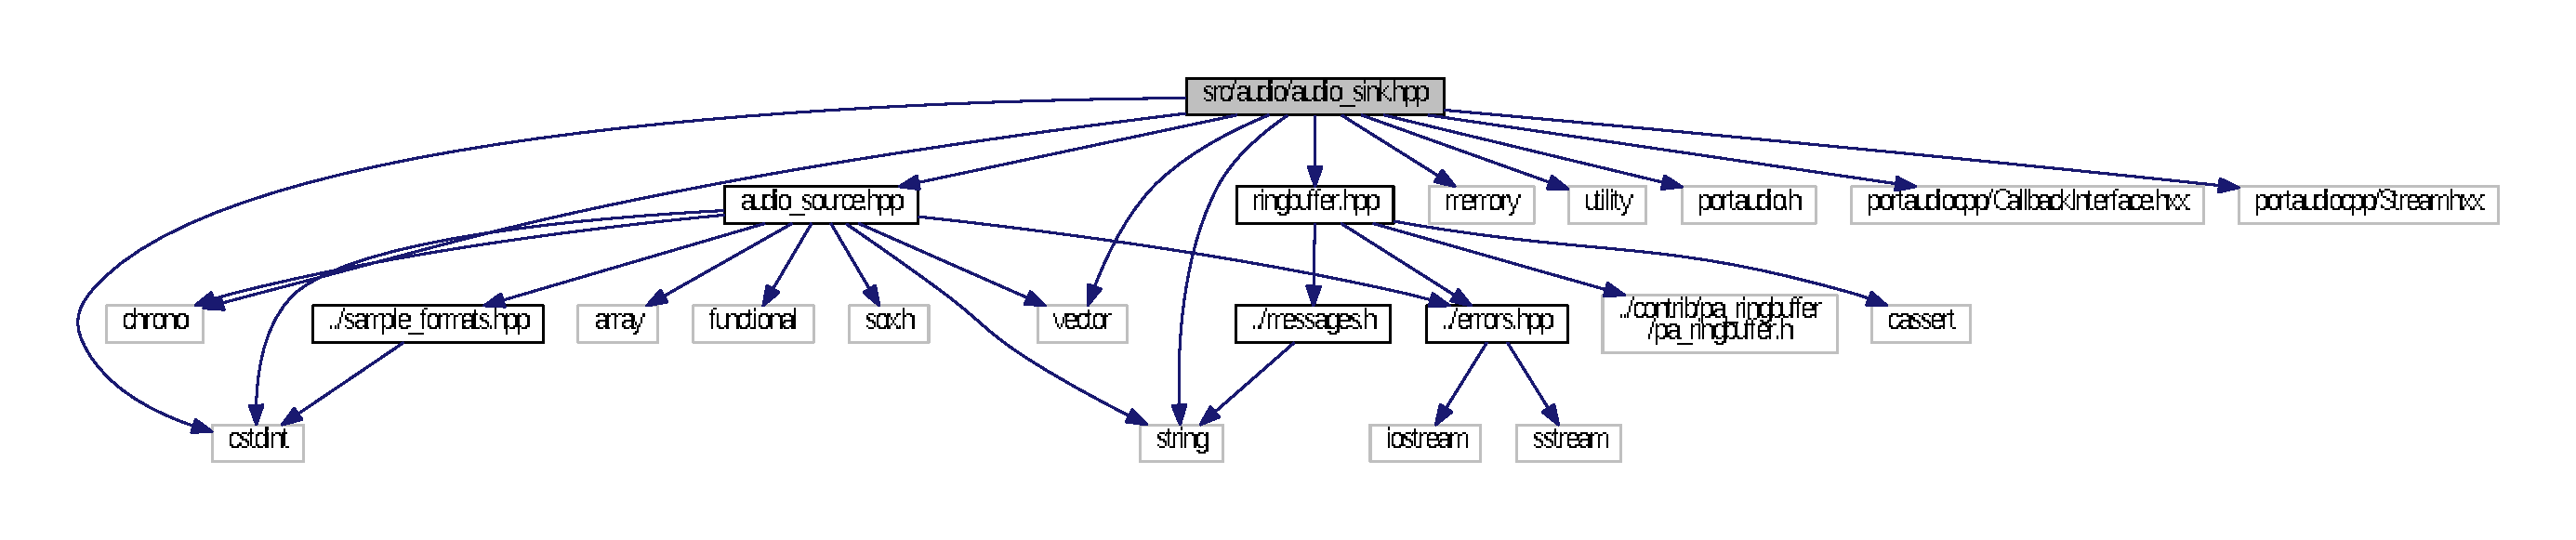
\includegraphics[width=350pt]{audio__sink_8hpp__incl}
\end{center}
\end{figure}
This graph shows which files directly or indirectly include this file\+:
\nopagebreak
\begin{figure}[H]
\begin{center}
\leavevmode
\includegraphics[width=350pt]{audio__sink_8hpp__dep__incl}
\end{center}
\end{figure}
\subsection*{Classes}
\begin{DoxyCompactItemize}
\item 
class \hyperlink{classAudioSink}{Audio\+Sink}
\begin{DoxyCompactList}\small\item\em An output stream for an \hyperlink{classAudio}{Audio} file. \end{DoxyCompactList}\end{DoxyCompactItemize}
\subsection*{Typedefs}
\begin{DoxyCompactItemize}
\item 
\hypertarget{audio__sink_8hpp_af1e317131d6c3a3f0adf7c5fca059d74}{using \hyperlink{audio__sink_8hpp_af1e317131d6c3a3f0adf7c5fca059d74}{Play\+Callback\+Step\+Result} = std\+::pair$<$ Pa\+Stream\+Callback\+Result, unsigned long $>$}\label{audio__sink_8hpp_af1e317131d6c3a3f0adf7c5fca059d74}

\begin{DoxyCompactList}\small\item\em Type of results emitted during the play callback step. \end{DoxyCompactList}\end{DoxyCompactItemize}


\subsection{Detailed Description}
Declaration of the \hyperlink{classAudioSink}{Audio\+Sink} class. 

\begin{DoxySeeAlso}{See also}
\hyperlink{audio_8cpp}{audio/audio.\+cpp} 
\end{DoxySeeAlso}


Definition in file \hyperlink{audio__sink_8hpp_source}{audio\+\_\+sink.\+hpp}.


\hypertarget{audio__sink_8hpp_source}{\section{audio\+\_\+sink.\+hpp}
\label{audio__sink_8hpp_source}\index{src/audio/audio\+\_\+sink.\+hpp@{src/audio/audio\+\_\+sink.\+hpp}}
}

\begin{DoxyCode}
00001 \textcolor{comment}{// This file is part of playd.}
00002 \textcolor{comment}{// playd is licenced under the MIT license: see LICENSE.txt.}
00003 
00010 \textcolor{preprocessor}{#ifndef PS\_AUDIO\_SINK\_HPP}
00011 \textcolor{preprocessor}{#define PS\_AUDIO\_SINK\_HPP}
00012 
00013 \textcolor{preprocessor}{#include <chrono>}
00014 \textcolor{preprocessor}{#include <cstdint>}
00015 \textcolor{preprocessor}{#include <memory>}
00016 \textcolor{preprocessor}{#include <string>}
00017 \textcolor{preprocessor}{#include <utility>}
00018 \textcolor{preprocessor}{#include <vector>}
00019 
00020 \textcolor{preprocessor}{#include "portaudio.h"}
00021 \textcolor{preprocessor}{#include "portaudiocpp/CallbackInterface.hxx"}
00022 \textcolor{preprocessor}{#include "portaudiocpp/Stream.hxx"}
00023 
00024 \textcolor{preprocessor}{#include "\hyperlink{audio__source_8hpp}{audio\_source.hpp}"}
00025 \textcolor{preprocessor}{#include "\hyperlink{ringbuffer_8hpp}{ringbuffer.hpp}"}
00026 
\hypertarget{audio__sink_8hpp_source_l00028}{}\hyperlink{audio__sink_8hpp_af1e317131d6c3a3f0adf7c5fca059d74}{00028} \textcolor{keyword}{using} \hyperlink{audio__sink_8hpp_af1e317131d6c3a3f0adf7c5fca059d74}{PlayCallbackStepResult} = std::pair<PaStreamCallbackResult, unsigned long>;
00029 
\hypertarget{audio__sink_8hpp_source_l00038}{}\hyperlink{classAudioSink}{00038} \textcolor{keyword}{class }\hyperlink{classAudioSink}{AudioSink} : portaudio::CallbackInterface \{
00039 \textcolor{keyword}{public}:
00042     \textcolor{keyword}{using} \hyperlink{classAudioSink_ae5b8370aa17c24c6fc8f8e0c5778168c}{StreamConfigurator} = std::function<
\hypertarget{audio__sink_8hpp_source_l00043}{}\hyperlink{classAudioSink_ae5b8370aa17c24c6fc8f8e0c5778168c}{00043}                     portaudio::Stream *(portaudio::CallbackInterface &)>;
00044 
00046     \textcolor{keyword}{using} \hyperlink{classAudioSink_a73002cc57611ac384c4e9d419e706e50}{PlayCallbackStepResult} =
\hypertarget{audio__sink_8hpp_source_l00047}{}\hyperlink{classAudioSink_a73002cc57611ac384c4e9d419e706e50}{00047}                     std::pair<PaStreamCallbackResult, unsigned long>;
00048 
\hypertarget{audio__sink_8hpp_source_l00050}{}\hyperlink{classAudioSink_ad2d7d33b3e937d057a4d72afad812737}{00050}     \textcolor{keyword}{using} \hyperlink{classAudioSink_ad2d7d33b3e937d057a4d72afad812737}{SamplePosition} = std::uint64\_t;
00051 
\hypertarget{audio__sink_8hpp_source_l00053}{}\hyperlink{classAudioSink_a60c1743d66e02b77f04791e72fa4cd0b}{00053}     \textcolor{keyword}{using} \hyperlink{classAudioSink_a60c1743d66e02b77f04791e72fa4cd0b}{TransferIterator} = AudioSource::DecodeVector::iterator;
00054 
00061     \hyperlink{classAudioSink_ab4adf46e3e93d35e2b5fb1ab0e75793b}{AudioSink}(\textcolor{keyword}{const} \hyperlink{classAudioSink_ae5b8370aa17c24c6fc8f8e0c5778168c}{StreamConfigurator} c,
00062               \hyperlink{classAudioSource_a1c8138ec9ffb9fd1394d0ad0782d60fa}{AudioSource::SampleByteCount} 
      \hyperlink{classAudioSink_a5eab0f7111187c0416feb542010e4a2e}{bytes\_per\_sample});
00063 
00069     \textcolor{keywordtype}{void} \hyperlink{classAudioSink_a18196e0dec3b4d58e17c454379ed0728}{Start}();
00070 
00076     \textcolor{keywordtype}{void} \hyperlink{classAudioSink_af1937ad09b555f0b88d285e8fd7cf433}{Stop}();
00077 
00084     \textcolor{keywordtype}{bool} \hyperlink{classAudioSink_adfa8006db0d1cbe161f15232cb32a324}{IsStopped}();
00085 
00093     \hyperlink{classAudioSink_ad2d7d33b3e937d057a4d72afad812737}{SamplePosition} \hyperlink{classAudioSink_aed168a8ce8ba39105431ab54ab08a007}{Position}();
00094 
00102     \textcolor{keywordtype}{void} \hyperlink{classAudioSink_a5ca539e3440d168eec0892114a947529}{SetPosition}(\hyperlink{classAudioSink_ad2d7d33b3e937d057a4d72afad812737}{SamplePosition} samples);
00103 
00109     \textcolor{keywordtype}{bool} \hyperlink{classAudioSink_a9b3dbe861acd4bb7ac1903730a0a01f3}{InputReady}();
00110 
00116     \textcolor{keywordtype}{void} \hyperlink{classAudioSink_aaa92237f7ab548c1a898981f4dcd631c}{SetInputReady}(\textcolor{keywordtype}{bool} ready);
00117 
00132     \textcolor{keywordtype}{void} \hyperlink{classAudioSink_a455e211f4f16eaa21e7b75412cc8a8ae}{Transfer}(\hyperlink{classAudioSink_a60c1743d66e02b77f04791e72fa4cd0b}{TransferIterator} &start, \textcolor{keyword}{const} 
      \hyperlink{classAudioSink_a60c1743d66e02b77f04791e72fa4cd0b}{TransferIterator} &end);
00133 
00134 \textcolor{keyword}{private}:
\hypertarget{audio__sink_8hpp_source_l00137}{}\hyperlink{classAudioSink_a152e5a388d4570211509a2a19a38c321}{00137}     \textcolor{keyword}{static} \textcolor{keyword}{const} \textcolor{keywordtype}{size\_t} \hyperlink{classAudioSink_a152e5a388d4570211509a2a19a38c321}{RINGBUF\_POWER};
00138 
\hypertarget{audio__sink_8hpp_source_l00140}{}\hyperlink{classAudioSink_a5eab0f7111187c0416feb542010e4a2e}{00140}     \hyperlink{classAudioSource_a1c8138ec9ffb9fd1394d0ad0782d60fa}{AudioSource::SampleByteCount} \hyperlink{classAudioSink_a5eab0f7111187c0416feb542010e4a2e}{bytes\_per\_sample};
00141 
\hypertarget{audio__sink_8hpp_source_l00143}{}\hyperlink{classAudioSink_a87184f85d6cfcc7310043b877caeaee2}{00143}     \hyperlink{classRingBuffer}{RingBuffer<char, unsigned long>} \hyperlink{classAudioSink_a87184f85d6cfcc7310043b877caeaee2}{ring\_buf};
00144 
\hypertarget{audio__sink_8hpp_source_l00146}{}\hyperlink{classAudioSink_aac90e7d95e98ac08b7c661a301eff1b2}{00146}     std::unique\_ptr<portaudio::Stream> \hyperlink{classAudioSink_aac90e7d95e98ac08b7c661a301eff1b2}{stream};
00147 
\hypertarget{audio__sink_8hpp_source_l00149}{}\hyperlink{classAudioSink_ac3403a492b8aba8d483961d1ec09fa26}{00149}     std::uint64\_t \hyperlink{classAudioSink_ac3403a492b8aba8d483961d1ec09fa26}{position\_sample\_count};
00150 
\hypertarget{audio__sink_8hpp_source_l00153}{}\hyperlink{classAudioSink_a00cbaaf2b4fcf5d9acb614b909234196}{00153}     \textcolor{keywordtype}{bool} \hyperlink{classAudioSink_a00cbaaf2b4fcf5d9acb614b909234196}{just\_started};
00154 
\hypertarget{audio__sink_8hpp_source_l00156}{}\hyperlink{classAudioSink_ad644a3477077e87f76cd24c9cb268f30}{00156}     \textcolor{keywordtype}{bool} \hyperlink{classAudioSink_ad644a3477077e87f76cd24c9cb268f30}{input\_ready};
00157 
00171     \textcolor{keywordtype}{int} \hyperlink{classAudioSink_ad3534ea4210aa83b42706c0361fd3e8d}{paCallbackFun}(\textcolor{keyword}{const} \textcolor{keywordtype}{void} *inputBuffer, \textcolor{keywordtype}{void} *outputBuffer,
00172                       \textcolor{keywordtype}{unsigned} \textcolor{keywordtype}{long} numFrames,
00173                       \textcolor{keyword}{const} PaStreamCallbackTimeInfo *timeInfo,
00174                       PaStreamCallbackFlags statusFlags) \textcolor{keyword}{override};
00175 
00185     \hyperlink{classAudioSink_a73002cc57611ac384c4e9d419e706e50}{PlayCallbackStepResult} \hyperlink{classAudioSink_a450ad1c0c64ddcc9b9a40d325983cbd9}{PlayCallbackStep}(\textcolor{keywordtype}{char} *out,
00186                                             \textcolor{keywordtype}{unsigned} \textcolor{keywordtype}{long} frames\_per\_buf,
00187                                             \hyperlink{classAudioSink_a73002cc57611ac384c4e9d419e706e50}{PlayCallbackStepResult} in);
00188 
00201     \hyperlink{classAudioSink_a73002cc57611ac384c4e9d419e706e50}{PlayCallbackStepResult} \hyperlink{classAudioSink_a2194fd0629b52c550c9eb326f8ae10cc}{PlayCallbackSuccess}(\textcolor{keywordtype}{char} *out,
00202                                                \textcolor{keywordtype}{unsigned} \textcolor{keywordtype}{long} avail,
00203                                                \textcolor{keywordtype}{unsigned} \textcolor{keywordtype}{long} frames\_per\_buf,
00204                                                \hyperlink{classAudioSink_a73002cc57611ac384c4e9d419e706e50}{PlayCallbackStepResult} in);
00205 
00218     \hyperlink{classAudioSink_a73002cc57611ac384c4e9d419e706e50}{PlayCallbackStepResult} \hyperlink{classAudioSink_a6e1b9254b242231ba8168e5e27d602ff}{PlayCallbackFailure}(\textcolor{keywordtype}{char} *out,
00219                                                \textcolor{keywordtype}{unsigned} \textcolor{keywordtype}{long} avail,
00220                                                \textcolor{keywordtype}{unsigned} \textcolor{keywordtype}{long} frames\_per\_buf,
00221                                                \hyperlink{classAudioSink_a73002cc57611ac384c4e9d419e706e50}{PlayCallbackStepResult} in);
00222 
00232     \textcolor{keywordtype}{unsigned} \textcolor{keywordtype}{long} \hyperlink{classAudioSink_a00ed918435d6f65b9533869453d5ae56}{ReadSamplesToOutput}(\textcolor{keywordtype}{char} *&output,
00233                                       \textcolor{keywordtype}{unsigned} \textcolor{keywordtype}{long} output\_capacity,
00234                                       \textcolor{keywordtype}{unsigned} \textcolor{keywordtype}{long} buffered\_count);
00235 \};
00236 
00237 \textcolor{preprocessor}{#endif // PS\_AUDIO\_SINK\_HPP}
\end{DoxyCode}

\hypertarget{audio__source_8cpp}{\section{src/audio/audio\+\_\+source.cpp File Reference}
\label{audio__source_8cpp}\index{src/audio/audio\+\_\+source.\+cpp@{src/audio/audio\+\_\+source.\+cpp}}
}


Implementation of the \hyperlink{classAudioSource}{Audio\+Source} class.  


{\ttfamily \#include $<$cassert$>$}\\*
{\ttfamily \#include $<$cstdint$>$}\\*
{\ttfamily \#include $<$cstdlib$>$}\\*
{\ttfamily \#include $<$functional$>$}\\*
{\ttfamily \#include $<$iostream$>$}\\*
{\ttfamily \#include $<$map$>$}\\*
{\ttfamily \#include $<$memory$>$}\\*
{\ttfamily \#include $<$sstream$>$}\\*
{\ttfamily \#include $<$string$>$}\\*
{\ttfamily \#include $<$sox.\+h$>$}\\*
{\ttfamily \#include \char`\"{}../errors.\+hpp\char`\"{}}\\*
{\ttfamily \#include \char`\"{}../messages.\+h\char`\"{}}\\*
{\ttfamily \#include \char`\"{}../sample\+\_\+formats.\+hpp\char`\"{}}\\*
{\ttfamily \#include \char`\"{}audio\+\_\+source.\+hpp\char`\"{}}\\*
Include dependency graph for audio\+\_\+source.\+cpp\+:
\nopagebreak
\begin{figure}[H]
\begin{center}
\leavevmode
\includegraphics[width=350pt]{audio__source_8cpp__incl}
\end{center}
\end{figure}


\subsection{Detailed Description}
Implementation of the \hyperlink{classAudioSource}{Audio\+Source} class. 

\begin{DoxySeeAlso}{See also}
\hyperlink{audio__source_8hpp}{audio/audio\+\_\+source.\+hpp} 
\end{DoxySeeAlso}


Definition in file \hyperlink{audio__source_8cpp_source}{audio\+\_\+source.\+cpp}.


\hypertarget{audio__source_8cpp_source}{\section{audio\+\_\+source.\+cpp}
\label{audio__source_8cpp_source}\index{src/audio/audio\+\_\+source.\+cpp@{src/audio/audio\+\_\+source.\+cpp}}
}

\begin{DoxyCode}
00001 \textcolor{comment}{// This file is part of playd.}
00002 \textcolor{comment}{// playd is licenced under the MIT license: see LICENSE.txt.}
00003 
00010 \textcolor{preprocessor}{#include <cassert>}
00011 \textcolor{preprocessor}{#include <cstdint>}
00012 \textcolor{preprocessor}{#include <cstdlib>}
00013 \textcolor{preprocessor}{#include <functional>}
00014 \textcolor{preprocessor}{#include <iostream>}
00015 \textcolor{preprocessor}{#include <map>}
00016 \textcolor{preprocessor}{#include <memory>}
00017 \textcolor{preprocessor}{#include <sstream>}
00018 \textcolor{preprocessor}{#include <string>}
00019 
00020 \textcolor{comment}{// libsox}
00021 \textcolor{keyword}{extern} \textcolor{stringliteral}{"C"} \{
00022 \textcolor{preprocessor}{#include <sox.h>}
00023 \}
00024 
00025 \textcolor{preprocessor}{#include "../errors.hpp"}
00026 \textcolor{preprocessor}{#include "../messages.h"}
00027 \textcolor{preprocessor}{#include "../sample\_formats.hpp"}
00028 \textcolor{preprocessor}{#include "\hyperlink{audio__source_8hpp}{audio\_source.hpp}"}
00029 
00030 \textcolor{comment}{// This value is somewhat arbitrary, but corresponds to the minimum buffer size}
00031 \textcolor{comment}{// used by ffmpeg, so it's probably sensible.}
00032 \textcolor{keyword}{const} \textcolor{keywordtype}{size\_t} \hyperlink{classAudioSource_a9c269c8d9c633bcd11d596c1ba3fd575}{AudioSource::BUFFER\_SIZE} = 16384;
00033 
\hypertarget{audio__source_8cpp_source_l00034}{}\hyperlink{classAudioSource_abcb925739a649c30663385a15d83af26}{00034} \hyperlink{classAudioSource_abcb925739a649c30663385a15d83af26}{AudioSource::AudioSource}(\textcolor{keyword}{const} std::string &path)
00035     : buffer(BUFFER\_SIZE), context(nullptr)
00036 \{
00037     \hyperlink{classAudioSource_a9b10234d7c9f29b17008b4dc3eab2a71}{Open}(path);
00038 \}
00039 
\hypertarget{audio__source_8cpp_source_l00040}{}\hyperlink{classAudioSource_a4d4b2be34ec676bf01d1ca1784f79a07}{00040} \hyperlink{classAudioSource_a4d4b2be34ec676bf01d1ca1784f79a07}{AudioSource::~AudioSource}()
00041 \{
00042     \hyperlink{classAudioSource_a46444de950d02ac35a695ad167fed2f4}{Close}();
00043 \}
00044 
\hypertarget{audio__source_8cpp_source_l00045}{}\hyperlink{classAudioSource_aea5c3828f1b22a9e103a5d56f9ffa5ec}{00045} std::string \hyperlink{classAudioSource_aea5c3828f1b22a9e103a5d56f9ffa5ec}{AudioSource::Path}()\textcolor{keyword}{ const}
00046 \textcolor{keyword}{}\{
00047     assert(this->\hyperlink{classAudioSource_a2bbce89d4bef9cf46b1113de3245655a}{context} != \textcolor{keyword}{nullptr});
00048     assert(this->\hyperlink{classAudioSource_a2bbce89d4bef9cf46b1113de3245655a}{context}->filename != \textcolor{keyword}{nullptr});
00049     \textcolor{keywordflow}{return} std::string(this->\hyperlink{classAudioSource_a2bbce89d4bef9cf46b1113de3245655a}{context}->filename);
00050 \}
00051 
\hypertarget{audio__source_8cpp_source_l00052}{}\hyperlink{classAudioSource_a267178b39a3a4d2fc86f41f6a96caf03}{00052} std::uint8\_t \hyperlink{classAudioSource_a267178b39a3a4d2fc86f41f6a96caf03}{AudioSource::ChannelCount}()\textcolor{keyword}{ const}
00053 \textcolor{keyword}{}\{
00054     assert(this->\hyperlink{classAudioSource_a2bbce89d4bef9cf46b1113de3245655a}{context} != \textcolor{keyword}{nullptr});
00055     \textcolor{keywordflow}{return} this->\hyperlink{classAudioSource_a2bbce89d4bef9cf46b1113de3245655a}{context}->signal.channels;
00056 \}
00057 
\hypertarget{audio__source_8cpp_source_l00058}{}\hyperlink{classAudioSource_af63c7249c1cf8d4ef86274ea2fdc1f26}{00058} \textcolor{keywordtype}{size\_t} \hyperlink{classAudioSource_af63c7249c1cf8d4ef86274ea2fdc1f26}{AudioSource::BufferSampleCapacity}()\textcolor{keyword}{ const}
00059 \textcolor{keyword}{}\{
00060     \textcolor{keywordflow}{return} this->\hyperlink{classAudioSource_ad278f3b315e3ad91add683d5eda48a03}{buffer}.size() / this->\hyperlink{classAudioSource_ae6eb4d0fc3d1d60375edc2745b635818}{BytesPerSample}();
00061 \}
00062 
\hypertarget{audio__source_8cpp_source_l00063}{}\hyperlink{classAudioSource_aee0c4889919554f3c947a217f4436378}{00063} \textcolor{keywordtype}{double} \hyperlink{classAudioSource_aee0c4889919554f3c947a217f4436378}{AudioSource::SampleRate}()\textcolor{keyword}{ const}
00064 \textcolor{keyword}{}\{
00065     assert(this->\hyperlink{classAudioSource_a2bbce89d4bef9cf46b1113de3245655a}{context} != \textcolor{keyword}{nullptr});
00066     \textcolor{keywordflow}{return} this->\hyperlink{classAudioSource_a2bbce89d4bef9cf46b1113de3245655a}{context}->signal.rate;
00067 \}
00068 
\hypertarget{audio__source_8cpp_source_l00069}{}\hyperlink{classAudioSource_ac0a5d14505c36238d4a8a465122ff06e}{00069} std::uint64\_t \hyperlink{classAudioSource_ac0a5d14505c36238d4a8a465122ff06e}{AudioSource::SamplePositionFromMicroseconds}(
00070                 std::chrono::microseconds usec)\textcolor{keyword}{ const}
00071 \textcolor{keyword}{}\{
00072     \textcolor{comment}{// The sample rate is expressed in terms of samples per second, so we}
00073     \textcolor{comment}{// need to convert the position to seconds then multiply by the rate.}
00074     \textcolor{comment}{// We do things in a slightly peculiar order to minimise rounding.}
00075 
00076     \textcolor{keyword}{auto} sample\_micros = usec * \hyperlink{classAudioSource_aee0c4889919554f3c947a217f4436378}{SampleRate}();
00077     \textcolor{keywordflow}{return} std::chrono::duration\_cast<std::chrono::seconds>(sample\_micros)
00078                     .count();
00079 \}
00080 
\hypertarget{audio__source_8cpp_source_l00081}{}\hyperlink{classAudioSource_aa9c0d4b60adfc1470a560bbb8e66aaf8}{00081} std::chrono::microseconds \hyperlink{classAudioSource_aa9c0d4b60adfc1470a560bbb8e66aaf8}{AudioSource::MicrosecondPositionFromSamples}
      (
00082                 std::uint64\_t samples)\textcolor{keyword}{ const}
00083 \textcolor{keyword}{}\{
00084     \textcolor{comment}{// This is basically SamplePositionFromMicroseconds but backwards.}
00085 
00086     \textcolor{keyword}{auto} position\_secs = std::chrono::seconds(samples) / \hyperlink{classAudioSource_aee0c4889919554f3c947a217f4436378}{SampleRate}();
00087     \textcolor{keywordflow}{return} std::chrono::duration\_cast<std::chrono::microseconds>(
00088                     position\_secs);
00089 \}
00090 
\hypertarget{audio__source_8cpp_source_l00091}{}\hyperlink{classAudioSource_ae6eb4d0fc3d1d60375edc2745b635818}{00091} \textcolor{keywordtype}{size\_t} \hyperlink{classAudioSource_ae6eb4d0fc3d1d60375edc2745b635818}{AudioSource::BytesPerSample}()\textcolor{keyword}{ const}
00092 \textcolor{keyword}{}\{
00093     assert(this->\hyperlink{classAudioSource_a2bbce89d4bef9cf46b1113de3245655a}{context} != \textcolor{keyword}{nullptr});
00094 
00095     \textcolor{comment}{// Since libsox always outputs 32-bit samples, the bytes per sample is}
00096     \textcolor{comment}{// always 4 per channel.}
00097 
00098     \textcolor{comment}{// SoX has a slightly peculiar notion of sample counts, in that it}
00099     \textcolor{comment}{// regards each channel as having its own separate sample, so we need}
00100     \textcolor{comment}{// to multiply and divide sample counts by the channel count when}
00101     \textcolor{comment}{// talking to SoX.}
00102     \textcolor{keywordflow}{return} 4 * \hyperlink{classAudioSource_a267178b39a3a4d2fc86f41f6a96caf03}{ChannelCount}();
00103 \}
00104 
\hypertarget{audio__source_8cpp_source_l00105}{}\hyperlink{classAudioSource_ad8639603fb59d21f5c1369707f16975c}{00105} std::uint64\_t \hyperlink{classAudioSource_ad8639603fb59d21f5c1369707f16975c}{AudioSource::Seek}(std::chrono::microseconds position)
00106 \{
00107     assert(this->\hyperlink{classAudioSource_a2bbce89d4bef9cf46b1113de3245655a}{context} != \textcolor{keyword}{nullptr});
00108 
00109     \textcolor{keyword}{auto} samples = \hyperlink{classAudioSource_ac0a5d14505c36238d4a8a465122ff06e}{SamplePositionFromMicroseconds}(position);
00110 
00111     \textcolor{comment}{// See BytesPerSample() for an explanation of this ChannelCount().}
00112     \textcolor{keyword}{auto} sox\_samples = samples * \hyperlink{classAudioSource_a267178b39a3a4d2fc86f41f6a96caf03}{ChannelCount}();
00113 
00114     \textcolor{comment}{// libsox doesn't seem to like seeking into an ended file, so close}
00115     \textcolor{comment}{// and re-open it first.}
00116     \textcolor{keywordflow}{if} (this->\hyperlink{classAudioSource_abe3899ebe685335a84c5bfee5a20a96f}{decode\_state} == \hyperlink{classAudioSource_a9a2f5de44325c84e69a7af1331aa159da581953f6b20ad7f993b64b1dc632032e}{DecodeState::END\_OF\_FILE}) \{
00117         std::string path = \hyperlink{classAudioSource_aea5c3828f1b22a9e103a5d56f9ffa5ec}{Path}();
00118         \hyperlink{classAudioSource_a46444de950d02ac35a695ad167fed2f4}{Close}();
00119         \hyperlink{classAudioSource_a9b10234d7c9f29b17008b4dc3eab2a71}{Open}(path);
00120     \}
00121 
00122     \textcolor{keywordflow}{if} (sox\_seek(this->\hyperlink{classAudioSource_a2bbce89d4bef9cf46b1113de3245655a}{context}, sox\_samples, SOX\_SEEK\_SET) != SOX\_SUCCESS) \{
00123         \textcolor{keywordflow}{throw} \hyperlink{classInternalError}{InternalError}(\hyperlink{messages_8h_aed3c894dfba47c4007dc39b38b5d3dbe}{MSG\_SEEK\_FAIL});
00124     \}
00125 
00126     \textcolor{comment}{// Reset the decoder state, because otherwise the decoder will get very}
00127     \textcolor{comment}{// confused.}
00128     this->\hyperlink{classAudioSource_abe3899ebe685335a84c5bfee5a20a96f}{decode\_state} = \hyperlink{classAudioSource_a9a2f5de44325c84e69a7af1331aa159da9b75f3acd3c3480965b0f5ee466e7f25}{DecodeState::DECODING};
00129 
00130     \textcolor{keywordflow}{return} samples;
00131 \}
00132 
\hypertarget{audio__source_8cpp_source_l00133}{}\hyperlink{classAudioSource_a6b5071168332523b68593bc47170f36f}{00133} \hyperlink{classAudioSource_aadbadeba50d982d09cfe0d1e05160ef9}{AudioSource::DecodeResult} \hyperlink{classAudioSource_a6b5071168332523b68593bc47170f36f}{AudioSource::Decode}()
00134 \{
00135     assert(this->\hyperlink{classAudioSource_a2bbce89d4bef9cf46b1113de3245655a}{context} != \textcolor{keyword}{nullptr});
00136 
00137     \textcolor{keyword}{auto} buf = \textcolor{keyword}{reinterpret\_cast<}sox\_sample\_t *\textcolor{keyword}{>}(&this->\hyperlink{classAudioSource_ad278f3b315e3ad91add683d5eda48a03}{buffer}.front());
00138 
00139     \textcolor{comment}{// See BytesPerSample() for an explanation of this ChannelCount().}
00140     \textcolor{keyword}{auto} sox\_capacity = \hyperlink{classAudioSource_af63c7249c1cf8d4ef86274ea2fdc1f26}{BufferSampleCapacity}() * 
      \hyperlink{classAudioSource_a267178b39a3a4d2fc86f41f6a96caf03}{ChannelCount}();
00141     \textcolor{keywordtype}{size\_t} read = sox\_read(this->\hyperlink{classAudioSource_a2bbce89d4bef9cf46b1113de3245655a}{context}, buf, sox\_capacity);
00142 
00143     \hyperlink{classAudioSource_a836c61e348dbe7df6ba255669c015303}{DecodeVector} decoded;
00144 
00145     \textcolor{keywordflow}{if} (read == 0) \{
00146         this->\hyperlink{classAudioSource_abe3899ebe685335a84c5bfee5a20a96f}{decode\_state} = \hyperlink{classAudioSource_a9a2f5de44325c84e69a7af1331aa159da581953f6b20ad7f993b64b1dc632032e}{DecodeState::END\_OF\_FILE};
00147     \} \textcolor{keywordflow}{else} \{
00148         this->\hyperlink{classAudioSource_abe3899ebe685335a84c5bfee5a20a96f}{decode\_state} = \hyperlink{classAudioSource_a9a2f5de44325c84e69a7af1331aa159da9b75f3acd3c3480965b0f5ee466e7f25}{DecodeState::DECODING};
00149 
00150         \textcolor{comment}{// Copy only the bit of the buffer occupied by decoded data}
00151         \textcolor{comment}{// See BytesPerSample() for an explanation of the}
00152         \textcolor{comment}{// ChannelCount() division.}
00153         \textcolor{keyword}{auto} front = this->\hyperlink{classAudioSource_ad278f3b315e3ad91add683d5eda48a03}{buffer}.begin();
00154         \textcolor{keyword}{auto} read\_bytes = (\hyperlink{classAudioSource_ae6eb4d0fc3d1d60375edc2745b635818}{BytesPerSample}() * read) / \hyperlink{classAudioSource_a267178b39a3a4d2fc86f41f6a96caf03}{ChannelCount}();
00155         decoded = \hyperlink{classAudioSource_a836c61e348dbe7df6ba255669c015303}{DecodeVector}(front, front + read\_bytes);
00156     \}
00157 
00158     \textcolor{keywordflow}{return} std::make\_pair(this->\hyperlink{classAudioSource_abe3899ebe685335a84c5bfee5a20a96f}{decode\_state}, decoded);
00159 \}
00160 
\hypertarget{audio__source_8cpp_source_l00164}{}\hyperlink{classAudioSource_aa6c567c4e2f3c6673d2a289d84aedae0}{00164} \hyperlink{sample__formats_8hpp_a21cca244e782ff3acc8805fb73236772}{SampleFormat} \hyperlink{classAudioSource_aa6c567c4e2f3c6673d2a289d84aedae0}{AudioSource::OutputSampleFormat}()\textcolor{keyword}{ const}
00165 \textcolor{keyword}{}\{
00166     \textcolor{comment}{// 'The function sox\_read reads len samples in to buf using the format}
00167     \textcolor{comment}{// handler specified by ft. All data read is converted to 32-bit signed}
00168     \textcolor{comment}{// samples before being placed in to buf.'}
00169     \textcolor{keywordflow}{return} \hyperlink{sample__formats_8hpp_a21cca244e782ff3acc8805fb73236772ae222eded89afdf8cf763bb1a58a04fc0}{SampleFormat::PACKED\_SIGNED\_INT\_32};
00170 \}
00171 
\hypertarget{audio__source_8cpp_source_l00172}{}\hyperlink{classAudioSource_a9b10234d7c9f29b17008b4dc3eab2a71}{00172} \textcolor{keywordtype}{void} \hyperlink{classAudioSource_a9b10234d7c9f29b17008b4dc3eab2a71}{AudioSource::Open}(\textcolor{keyword}{const} std::string &path)
00173 \{
00174     \hyperlink{classAudioSource_a46444de950d02ac35a695ad167fed2f4}{Close}();
00175 
00176     this->\hyperlink{classAudioSource_a2bbce89d4bef9cf46b1113de3245655a}{context} = sox\_open\_read(path.c\_str(), \textcolor{keyword}{nullptr}, \textcolor{keyword}{nullptr}, \textcolor{keyword}{nullptr});
00177     \textcolor{keywordflow}{if} (this->\hyperlink{classAudioSource_a2bbce89d4bef9cf46b1113de3245655a}{context} == \textcolor{keyword}{nullptr}) \{
00178         std::ostringstream os;
00179         os << \textcolor{stringliteral}{"couldn't open "} << path;
00180         \textcolor{keywordflow}{throw} \hyperlink{classFileError}{FileError}(os.str());
00181     \}
00182 \}
00183 
\hypertarget{audio__source_8cpp_source_l00184}{}\hyperlink{classAudioSource_a46444de950d02ac35a695ad167fed2f4}{00184} \textcolor{keywordtype}{void} \hyperlink{classAudioSource_a46444de950d02ac35a695ad167fed2f4}{AudioSource::Close}()
00185 \{
00186     \textcolor{keywordflow}{if} (this->\hyperlink{classAudioSource_a2bbce89d4bef9cf46b1113de3245655a}{context} != \textcolor{keyword}{nullptr}) \{
00187         sox\_close(this->\hyperlink{classAudioSource_a2bbce89d4bef9cf46b1113de3245655a}{context});
00188         this->\hyperlink{classAudioSource_a2bbce89d4bef9cf46b1113de3245655a}{context} = \textcolor{keyword}{nullptr};
00189     \}
00190 \}
\end{DoxyCode}

\hypertarget{audio__source_8hpp}{\section{src/audio/audio\+\_\+source.hpp File Reference}
\label{audio__source_8hpp}\index{src/audio/audio\+\_\+source.\+hpp@{src/audio/audio\+\_\+source.\+hpp}}
}


Declaration of the \hyperlink{classAudioSource}{Audio\+Source} class.  


{\ttfamily \#include $<$array$>$}\\*
{\ttfamily \#include $<$chrono$>$}\\*
{\ttfamily \#include $<$cstdint$>$}\\*
{\ttfamily \#include $<$functional$>$}\\*
{\ttfamily \#include $<$string$>$}\\*
{\ttfamily \#include $<$vector$>$}\\*
{\ttfamily \#include $<$sox.\+h$>$}\\*
{\ttfamily \#include \char`\"{}../errors.\+hpp\char`\"{}}\\*
{\ttfamily \#include \char`\"{}../sample\+\_\+formats.\+hpp\char`\"{}}\\*
Include dependency graph for audio\+\_\+source.\+hpp\+:
\nopagebreak
\begin{figure}[H]
\begin{center}
\leavevmode
\includegraphics[width=350pt]{audio__source_8hpp__incl}
\end{center}
\end{figure}
This graph shows which files directly or indirectly include this file\+:
\nopagebreak
\begin{figure}[H]
\begin{center}
\leavevmode
\includegraphics[width=350pt]{audio__source_8hpp__dep__incl}
\end{center}
\end{figure}
\subsection*{Classes}
\begin{DoxyCompactItemize}
\item 
class \hyperlink{classAudioSource}{Audio\+Source}
\begin{DoxyCompactList}\small\item\em An object responsible for decoding an audio file. \end{DoxyCompactList}\end{DoxyCompactItemize}


\subsection{Detailed Description}
Declaration of the \hyperlink{classAudioSource}{Audio\+Source} class. 

\begin{DoxySeeAlso}{See also}
\hyperlink{audio__source_8cpp}{audio/audio\+\_\+source.\+cpp} 
\end{DoxySeeAlso}


Definition in file \hyperlink{audio__source_8hpp_source}{audio\+\_\+source.\+hpp}.


\hypertarget{audio__source_8hpp_source}{\section{audio\+\_\+source.\+hpp}
\label{audio__source_8hpp_source}\index{src/audio/audio\+\_\+source.\+hpp@{src/audio/audio\+\_\+source.\+hpp}}
}

\begin{DoxyCode}
00001 \textcolor{comment}{// This file is part of playd.}
00002 \textcolor{comment}{// playd is licenced under the MIT license: see LICENSE.txt.}
00003 
00010 \textcolor{preprocessor}{#ifndef PS\_AUDIO\_SOURCE\_HPP}
00011 \textcolor{preprocessor}{#define PS\_AUDIO\_SOURCE\_HPP}
00012 
00013 \textcolor{preprocessor}{#include <array>}
00014 \textcolor{preprocessor}{#include <chrono>}
00015 \textcolor{preprocessor}{#include <cstdint>}
00016 \textcolor{preprocessor}{#include <functional>}
00017 \textcolor{preprocessor}{#include <string>}
00018 \textcolor{preprocessor}{#include <vector>}
00019 
00020 \textcolor{preprocessor}{#include <sox.h>}
00021 
00022 \textcolor{preprocessor}{#include "../errors.hpp"}
00023 \textcolor{preprocessor}{#include "../sample\_formats.hpp"}
00024 
\hypertarget{audio__source_8hpp_source_l00032}{}\hyperlink{classAudioSource}{00032} \textcolor{keyword}{class }\hyperlink{classAudioSource}{AudioSource} \{
00033 \textcolor{keyword}{public}:
\hypertarget{audio__source_8hpp_source_l00035}{}\hyperlink{classAudioSource_a9a2f5de44325c84e69a7af1331aa159d}{00035}     \textcolor{keyword}{enum class} \hyperlink{classAudioSource_a9a2f5de44325c84e69a7af1331aa159d}{DecodeState} : std::uint8\_t \{
00037         \hyperlink{classAudioSource_a9a2f5de44325c84e69a7af1331aa159da22a62bc6e9b3fff5866c4259f046bad8}{WAITING\_FOR\_FRAME},
00039         \hyperlink{classAudioSource_a9a2f5de44325c84e69a7af1331aa159da9b75f3acd3c3480965b0f5ee466e7f25}{DECODING},
00041         \hyperlink{classAudioSource_a9a2f5de44325c84e69a7af1331aa159da581953f6b20ad7f993b64b1dc632032e}{END\_OF\_FILE}
00042     \};
00043 
\hypertarget{audio__source_8hpp_source_l00045}{}\hyperlink{classAudioSource_a836c61e348dbe7df6ba255669c015303}{00045}     \textcolor{keyword}{using} \hyperlink{classAudioSource_a836c61e348dbe7df6ba255669c015303}{DecodeVector} = std::vector<std::uint8\_t>;
00046 
\hypertarget{audio__source_8hpp_source_l00048}{}\hyperlink{classAudioSource_aadbadeba50d982d09cfe0d1e05160ef9}{00048}     \textcolor{keyword}{using} \hyperlink{classAudioSource_aadbadeba50d982d09cfe0d1e05160ef9}{DecodeResult} = std::pair<DecodeState, DecodeVector>;
00049 
\hypertarget{audio__source_8hpp_source_l00051}{}\hyperlink{classAudioSource_a1c8138ec9ffb9fd1394d0ad0782d60fa}{00051}     \textcolor{keyword}{using} \hyperlink{classAudioSource_a1c8138ec9ffb9fd1394d0ad0782d60fa}{SampleByteCount} = int;
00052 
00058     \hyperlink{classAudioSource_abcb925739a649c30663385a15d83af26}{AudioSource}(\textcolor{keyword}{const} std::string &path);
00059 
00061     \hyperlink{classAudioSource_a4d4b2be34ec676bf01d1ca1784f79a07}{~AudioSource}();
00062 
00067     std::string \hyperlink{classAudioSource_aea5c3828f1b22a9e103a5d56f9ffa5ec}{Path}() \textcolor{keyword}{const};
00068 
00075     \hyperlink{classAudioSource_aadbadeba50d982d09cfe0d1e05160ef9}{DecodeResult} \hyperlink{classAudioSource_a6b5071168332523b68593bc47170f36f}{Decode}();
00076 
00081     std::uint8\_t \hyperlink{classAudioSource_a267178b39a3a4d2fc86f41f6a96caf03}{ChannelCount}() \textcolor{keyword}{const};
00082 
00088     \textcolor{keywordtype}{double} \hyperlink{classAudioSource_aee0c4889919554f3c947a217f4436378}{SampleRate}() \textcolor{keyword}{const};
00089 
00094     \hyperlink{sample__formats_8hpp_a21cca244e782ff3acc8805fb73236772}{SampleFormat} \hyperlink{classAudioSource_aa6c567c4e2f3c6673d2a289d84aedae0}{OutputSampleFormat}() \textcolor{keyword}{const};
00095 
00100     \textcolor{keywordtype}{size\_t} \hyperlink{classAudioSource_af63c7249c1cf8d4ef86274ea2fdc1f26}{BufferSampleCapacity}() \textcolor{keyword}{const};
00101 
00108     \textcolor{keywordtype}{size\_t} \hyperlink{classAudioSource_ae6eb4d0fc3d1d60375edc2745b635818}{BytesPerSample}() \textcolor{keyword}{const};
00109 
00116     std::uint64\_t \hyperlink{classAudioSource_ad8639603fb59d21f5c1369707f16975c}{Seek}(std::chrono::microseconds position);
00117 
00123     std::uint64\_t \hyperlink{classAudioSource_ac0a5d14505c36238d4a8a465122ff06e}{SamplePositionFromMicroseconds}(
00124                     std::chrono::microseconds position) \textcolor{keyword}{const};
00125 
00131     std::chrono::microseconds \hyperlink{classAudioSource_aa9c0d4b60adfc1470a560bbb8e66aaf8}{MicrosecondPositionFromSamples}(
00132                     std::uint64\_t samples) \textcolor{keyword}{const};
00133 
00134 \textcolor{keyword}{private}:
\hypertarget{audio__source_8hpp_source_l00136}{}\hyperlink{classAudioSource_a9c269c8d9c633bcd11d596c1ba3fd575}{00136}     \textcolor{keyword}{static} \textcolor{keyword}{const} \textcolor{keywordtype}{size\_t} \hyperlink{classAudioSource_a9c269c8d9c633bcd11d596c1ba3fd575}{BUFFER\_SIZE};
00137 
\hypertarget{audio__source_8hpp_source_l00140}{}\hyperlink{classAudioSource_abe3899ebe685335a84c5bfee5a20a96f}{00140}     \hyperlink{classAudioSource_a9a2f5de44325c84e69a7af1331aa159d}{DecodeState} \hyperlink{classAudioSource_abe3899ebe685335a84c5bfee5a20a96f}{decode\_state};
00141 
\hypertarget{audio__source_8hpp_source_l00142}{}\hyperlink{classAudioSource_ad278f3b315e3ad91add683d5eda48a03}{00142}     std::vector<uint8\_t> \hyperlink{classAudioSource_ad278f3b315e3ad91add683d5eda48a03}{buffer}; 
00143 
\hypertarget{audio__source_8hpp_source_l00145}{}\hyperlink{classAudioSource_a2bbce89d4bef9cf46b1113de3245655a}{00145}     sox\_format\_t *\hyperlink{classAudioSource_a2bbce89d4bef9cf46b1113de3245655a}{context};
00146 
00151     \textcolor{keywordtype}{void} \hyperlink{classAudioSource_a9b10234d7c9f29b17008b4dc3eab2a71}{Open}(\textcolor{keyword}{const} std::string &path);
00152 
00154     \textcolor{keywordtype}{void} \hyperlink{classAudioSource_a46444de950d02ac35a695ad167fed2f4}{Close}();
00155 \};
00156 
00157 \textcolor{preprocessor}{#endif // PS\_AUDIO\_SOURCE\_HPP}
\end{DoxyCode}

\hypertarget{audio__system_8cpp}{\section{src/audio/audio\+\_\+system.cpp File Reference}
\label{audio__system_8cpp}\index{src/audio/audio\+\_\+system.\+cpp@{src/audio/audio\+\_\+system.\+cpp}}
}


Implementation of the \hyperlink{classAudioSystem}{Audio\+System} class.  


{\ttfamily \#include $<$algorithm$>$}\\*
{\ttfamily \#include $<$map$>$}\\*
{\ttfamily \#include $<$sstream$>$}\\*
{\ttfamily \#include $<$stdexcept$>$}\\*
{\ttfamily \#include $<$string$>$}\\*
{\ttfamily \#include $<$sox.\+h$>$}\\*
{\ttfamily \#include \char`\"{}portaudio.\+h\char`\"{}}\\*
{\ttfamily \#include \char`\"{}portaudiocpp/\+Device.\+hxx\char`\"{}}\\*
{\ttfamily \#include \char`\"{}portaudiocpp/\+Direction\+Specific\+Stream\+Parameters.\+hxx\char`\"{}}\\*
{\ttfamily \#include \char`\"{}portaudiocpp/\+Interface\+Callback\+Stream.\+hxx\char`\"{}}\\*
{\ttfamily \#include \char`\"{}portaudiocpp/\+Sample\+Data\+Format.\+hxx\char`\"{}}\\*
{\ttfamily \#include \char`\"{}portaudiocpp/\+Stream.\+hxx\char`\"{}}\\*
{\ttfamily \#include \char`\"{}portaudiocpp/\+Stream\+Parameters.\+hxx\char`\"{}}\\*
{\ttfamily \#include \char`\"{}portaudiocpp/\+System.\+hxx\char`\"{}}\\*
{\ttfamily \#include \char`\"{}portaudiocpp/\+System\+Device\+Iterator.\+hxx\char`\"{}}\\*
{\ttfamily \#include \char`\"{}../errors.\+hpp\char`\"{}}\\*
{\ttfamily \#include \char`\"{}../messages.\+h\char`\"{}}\\*
{\ttfamily \#include \char`\"{}../sample\+\_\+formats.\+hpp\char`\"{}}\\*
{\ttfamily \#include \char`\"{}audio.\+hpp\char`\"{}}\\*
{\ttfamily \#include \char`\"{}audio\+\_\+sink.\+hpp\char`\"{}}\\*
{\ttfamily \#include \char`\"{}audio\+\_\+source.\+hpp\char`\"{}}\\*
{\ttfamily \#include \char`\"{}audio\+\_\+system.\+hpp\char`\"{}}\\*
Include dependency graph for audio\+\_\+system.\+cpp\+:
\nopagebreak
\begin{figure}[H]
\begin{center}
\leavevmode
\includegraphics[width=350pt]{audio__system_8cpp__incl}
\end{center}
\end{figure}


\subsection{Detailed Description}
Implementation of the \hyperlink{classAudioSystem}{Audio\+System} class. 

\begin{DoxySeeAlso}{See also}
\hyperlink{audio__system_8hpp}{audio/audio\+\_\+system.\+hpp} 
\end{DoxySeeAlso}


Definition in file \hyperlink{audio__system_8cpp_source}{audio\+\_\+system.\+cpp}.


\hypertarget{audio__system_8cpp_source}{\section{audio\+\_\+system.\+cpp}
\label{audio__system_8cpp_source}\index{src/audio/audio\+\_\+system.\+cpp@{src/audio/audio\+\_\+system.\+cpp}}
}

\begin{DoxyCode}
00001 \textcolor{comment}{// This file is part of playd.}
00002 \textcolor{comment}{// playd is licenced under the MIT license: see LICENSE.txt.}
00003 
00010 \textcolor{preprocessor}{#include <algorithm>}
00011 \textcolor{preprocessor}{#include <map>}
00012 \textcolor{preprocessor}{#include <sstream>}
00013 \textcolor{preprocessor}{#include <stdexcept>}
00014 \textcolor{preprocessor}{#include <string>}
00015 
00016 \textcolor{keyword}{extern} \textcolor{stringliteral}{"C"} \{
00017 \textcolor{preprocessor}{#include <sox.h>}
00018 \textcolor{preprocessor}{#include "portaudio.h"}
00019 \}
00020 
00021 \textcolor{preprocessor}{#include "portaudiocpp/Device.hxx"}
00022 \textcolor{preprocessor}{#include "portaudiocpp/DirectionSpecificStreamParameters.hxx"}
00023 \textcolor{preprocessor}{#include "portaudiocpp/InterfaceCallbackStream.hxx"}
00024 \textcolor{preprocessor}{#include "portaudiocpp/SampleDataFormat.hxx"}
00025 \textcolor{preprocessor}{#include "portaudiocpp/Stream.hxx"}
00026 \textcolor{preprocessor}{#include "portaudiocpp/StreamParameters.hxx"}
00027 \textcolor{preprocessor}{#include "portaudiocpp/System.hxx"}
00028 \textcolor{preprocessor}{#include "portaudiocpp/SystemDeviceIterator.hxx"}
00029 \textcolor{keyword}{namespace }portaudio \{
00030 \textcolor{keyword}{class }CallbackInterface;
00031 \}
00032 
00033 \textcolor{preprocessor}{#include "../errors.hpp"}
00034 \textcolor{preprocessor}{#include "../messages.h"}
00035 \textcolor{preprocessor}{#include "../sample\_formats.hpp"}
00036 \textcolor{preprocessor}{#include "\hyperlink{audio_8hpp}{audio.hpp}"}
00037 \textcolor{preprocessor}{#include "\hyperlink{audio__sink_8hpp}{audio\_sink.hpp}"}
00038 \textcolor{preprocessor}{#include "\hyperlink{audio__source_8hpp}{audio\_source.hpp}"}
00039 \textcolor{preprocessor}{#include "\hyperlink{audio__system_8hpp}{audio\_system.hpp}"}
00040 
\hypertarget{audio__system_8cpp_source_l00041}{}\hyperlink{classAudioSystem_ad17cde8deff07ef7d7d56be62df98739}{00041} \hyperlink{classAudioSystem_ad17cde8deff07ef7d7d56be62df98739}{AudioSystem::AudioSystem}()
00042 \{
00043     portaudio::System::initialize();
00044     sox\_format\_init();
00045 
00046     this->\hyperlink{classAudioSystem_a3071e6d8643b3d0275ba63820e6e0072}{device\_id} = -1;
00047 \}
00048 
\hypertarget{audio__system_8cpp_source_l00049}{}\hyperlink{classAudioSystem_a9ad830040ea5f68a6a63957c6f281055}{00049} \hyperlink{classAudioSystem_a9ad830040ea5f68a6a63957c6f281055}{AudioSystem::~AudioSystem}()
00050 \{
00051     portaudio::System::terminate();
00052     sox\_format\_quit();
00053 \}
00054 
\hypertarget{audio__system_8cpp_source_l00055}{}\hyperlink{classAudioSystem_aa268faeb9243c18588631024958856e6}{00055} std::vector<AudioSystem::Device> \hyperlink{classAudioSystem_aa268faeb9243c18588631024958856e6}{AudioSystem::GetDevicesInfo}()
00056 \{
00057     \textcolor{keyword}{auto} &pa = portaudio::System::instance();
00058     std::vector<AudioSystem::Device> list;
00059 
00060     \textcolor{keywordflow}{for} (\textcolor{keyword}{auto} d = pa.devicesBegin(); d != pa.devicesEnd(); ++d) \{
00061         \textcolor{keywordflow}{if} (!(*d).isInputOnlyDevice()) \{
00062             list.push\_back(std::make\_pair((*d).index(),
00063                                           (*d).name()));
00064         \}
00065     \}
00066     \textcolor{keywordflow}{return} list;
00067 \}
00068 
\hypertarget{audio__system_8cpp_source_l00069}{}\hyperlink{classAudioSystem_a001cd82f854883b80b3ed7d35795581b}{00069} \textcolor{keywordtype}{bool} \hyperlink{classAudioSystem_a001cd82f854883b80b3ed7d35795581b}{AudioSystem::IsOutputDevice}(\textcolor{keywordtype}{int} \textcolor{keywordtype}{id})
00070 \{
00071     \textcolor{keyword}{auto} &pa = portaudio::System::instance();
00072     \textcolor{keywordflow}{if} (id < 0 || id >= pa.deviceCount()) \textcolor{keywordflow}{return} \textcolor{keyword}{false};
00073 
00074     portaudio::Device &dev = pa.deviceByIndex(\textcolor{keywordtype}{id});
00075     \textcolor{keywordflow}{return} !dev.isInputOnlyDevice();
00076 \}
00077 
\hypertarget{audio__system_8cpp_source_l00078}{}\hyperlink{classAudioSystem_ade3b400828991d02e36a0b61302d30d2}{00078} \textcolor{keywordtype}{void} \hyperlink{classAudioSystem_ade3b400828991d02e36a0b61302d30d2}{AudioSystem::SetDeviceID}(\textcolor{keywordtype}{int} \textcolor{keywordtype}{id})
00079 \{
00080     this->\hyperlink{classAudioSystem_a3071e6d8643b3d0275ba63820e6e0072}{device\_id} = std::to\_string(\textcolor{keywordtype}{id});
00081 \}
00082 
\hypertarget{audio__system_8cpp_source_l00083}{}\hyperlink{classAudioSystem_a2172608177d2bd54377bfc3c61cd117d}{00083} \hyperlink{classAudio}{Audio} *\hyperlink{classAudioSystem_a2172608177d2bd54377bfc3c61cd117d}{AudioSystem::Load}(\textcolor{keyword}{const} std::string &path)\textcolor{keyword}{ const}
00084 \textcolor{keyword}{}\{
00085     \textcolor{keyword}{auto} source = \textcolor{keyword}{new} \hyperlink{classAudioSource}{AudioSource}(path);
00086 
00087     \hyperlink{classAudioSink_ae5b8370aa17c24c6fc8f8e0c5778168c}{AudioSink::StreamConfigurator} config\_fn = std::bind(
00088                     &\hyperlink{classAudioSystem_a78e8754440e0a29f5fac9ca1cd79a109}{AudioSystem::Configure}, \textcolor{keyword}{this}, source->ChannelCount(),
00089                     source->OutputSampleFormat(), source->SampleRate(),
00090                     source->BufferSampleCapacity(), std::placeholders::\_1);
00091     \textcolor{keyword}{auto} sink = \textcolor{keyword}{new} \hyperlink{classAudioSink}{AudioSink}(config\_fn, source->BytesPerSample());
00092 
00093     \textcolor{keywordflow}{return} \textcolor{keyword}{new} \hyperlink{classAudio}{Audio}(source, sink);
00094 \}
00095 
\hypertarget{audio__system_8cpp_source_l00096}{}\hyperlink{classAudioSystem_a78e8754440e0a29f5fac9ca1cd79a109}{00096} portaudio::Stream *\hyperlink{classAudioSystem_a78e8754440e0a29f5fac9ca1cd79a109}{AudioSystem::Configure}(
00097                 std::uint8\_t channel\_count, \hyperlink{sample__formats_8hpp_a21cca244e782ff3acc8805fb73236772}{SampleFormat} sample\_format,
00098                 \textcolor{keywordtype}{double} sample\_rate, \textcolor{keywordtype}{size\_t} buffer\_size,
00099                 portaudio::CallbackInterface &cb)\textcolor{keyword}{ const}
00100 \textcolor{keyword}{}\{
00101     \textcolor{keyword}{const} portaudio::Device &device = \hyperlink{classAudioSystem_a513a0de4748574e25cba443f28949a90}{PaDeviceFrom}(this->\hyperlink{classAudioSystem_a3071e6d8643b3d0275ba63820e6e0072}{device\_id});
00102 
00103     portaudio::DirectionSpecificStreamParameters out\_pars(
00104                     device, channel\_count,
00105                     \hyperlink{classAudioSystem_aac640b14ad80c2518539bcafe9f4b5ac}{PaSampleFormatFrom}(sample\_format), \textcolor{keyword}{true},
00106                     device.defaultLowOutputLatency(), \textcolor{keyword}{nullptr});
00107 
00108     portaudio::StreamParameters pars(
00109                     portaudio::DirectionSpecificStreamParameters::null(),
00110                     out\_pars, sample\_rate, buffer\_size, paClipOff);
00111 
00112     \textcolor{keywordflow}{return} \textcolor{keyword}{new} portaudio::InterfaceCallbackStream(pars, cb);
00113 \}
00114 
\hypertarget{audio__system_8cpp_source_l00115}{}\hyperlink{classAudioSystem_a513a0de4748574e25cba443f28949a90}{00115} \textcolor{keyword}{const} portaudio::Device &\hyperlink{classAudioSystem_a513a0de4748574e25cba443f28949a90}{AudioSystem::PaDeviceFrom}(\textcolor{keyword}{const} std::string &id\_string)\textcolor{keyword}{}
00116 \textcolor{keyword}{                const}
00117 \textcolor{keyword}{}\{
00118     \textcolor{keyword}{auto} &pa = portaudio::System::instance();
00119 
00120     PaDeviceIndex id\_pa = 0;
00121 
00122     std::istringstream is(id\_string);
00123     is >> id\_pa;
00124 
00125     \textcolor{keywordflow}{if} (id\_pa >= pa.deviceCount()) \{
00126         \textcolor{keywordflow}{throw} \hyperlink{classConfigError}{ConfigError}(\hyperlink{messages_8h_a80a8cb0d00a63114c8c5c8228fa39ec4}{MSG\_DEV\_BADID});
00127     \}
00128 
00129     \textcolor{keywordflow}{return} pa.deviceByIndex(id\_pa);
00130 \}
00131 
00133 \textcolor{keyword}{static} \textcolor{keyword}{const} std::map<SampleFormat, portaudio::SampleDataFormat> pa\_from\_sf = \{
00134     \{ \hyperlink{sample__formats_8hpp_a21cca244e782ff3acc8805fb73236772a0f083be5e0e503eb0830e26687f00cf2}{SampleFormat::PACKED\_UNSIGNED\_INT\_8}, portaudio::UINT8 \},
00135     \{ \hyperlink{sample__formats_8hpp_a21cca244e782ff3acc8805fb73236772a3bc6c5371607364846832278d3d39965}{SampleFormat::PACKED\_SIGNED\_INT\_16}, portaudio::INT16 \},
00136     \{ \hyperlink{sample__formats_8hpp_a21cca244e782ff3acc8805fb73236772ae222eded89afdf8cf763bb1a58a04fc0}{SampleFormat::PACKED\_SIGNED\_INT\_32}, portaudio::INT32 \},
00137     \{ \hyperlink{sample__formats_8hpp_a21cca244e782ff3acc8805fb73236772ae58d6feb65720ac0b7e1158a2debcf7d}{SampleFormat::PACKED\_FLOAT\_32}, portaudio::FLOAT32 \}
00138 \};
00139 
\hypertarget{audio__system_8cpp_source_l00140}{}\hyperlink{classAudioSystem_aac640b14ad80c2518539bcafe9f4b5ac}{00140} portaudio::SampleDataFormat \hyperlink{classAudioSystem_aac640b14ad80c2518539bcafe9f4b5ac}{AudioSystem::PaSampleFormatFrom}(
      \hyperlink{sample__formats_8hpp_a21cca244e782ff3acc8805fb73236772}{SampleFormat} fmt)\textcolor{keyword}{}
00141 \textcolor{keyword}{                const}
00142 \textcolor{keyword}{}\{
00143     \textcolor{keywordflow}{try}
00144     \{
00145         \textcolor{keywordflow}{return} pa\_from\_sf.at(fmt);
00146     \}
00147     \textcolor{keywordflow}{catch} (std::out\_of\_range)
00148     \{
00149         \textcolor{keywordflow}{throw} \hyperlink{classFileError}{FileError}(\hyperlink{messages_8h_a6d4302117e822520f5c61b6d40085c4d}{MSG\_DECODE\_BADRATE});
00150     \}
00151 \}
\end{DoxyCode}

\hypertarget{audio__system_8hpp}{\section{src/audio/audio\+\_\+system.hpp File Reference}
\label{audio__system_8hpp}\index{src/audio/audio\+\_\+system.\+hpp@{src/audio/audio\+\_\+system.\+hpp}}
}


Declaration of the \hyperlink{classAudioSystem}{Audio\+System} class.  


{\ttfamily \#include $<$functional$>$}\\*
{\ttfamily \#include $<$string$>$}\\*
{\ttfamily \#include $<$utility$>$}\\*
{\ttfamily \#include \char`\"{}portaudiocpp/\+Sample\+Data\+Format.\+hxx\char`\"{}}\\*
{\ttfamily \#include \char`\"{}portaudiocpp/\+Stream.\+hxx\char`\"{}}\\*
{\ttfamily \#include \char`\"{}../sample\+\_\+formats.\+hpp\char`\"{}}\\*
{\ttfamily \#include \char`\"{}audio\+\_\+sink.\+hpp\char`\"{}}\\*
{\ttfamily \#include \char`\"{}audio\+\_\+source.\+hpp\char`\"{}}\\*
{\ttfamily \#include \char`\"{}audio.\+hpp\char`\"{}}\\*
Include dependency graph for audio\+\_\+system.\+hpp\+:
\nopagebreak
\begin{figure}[H]
\begin{center}
\leavevmode
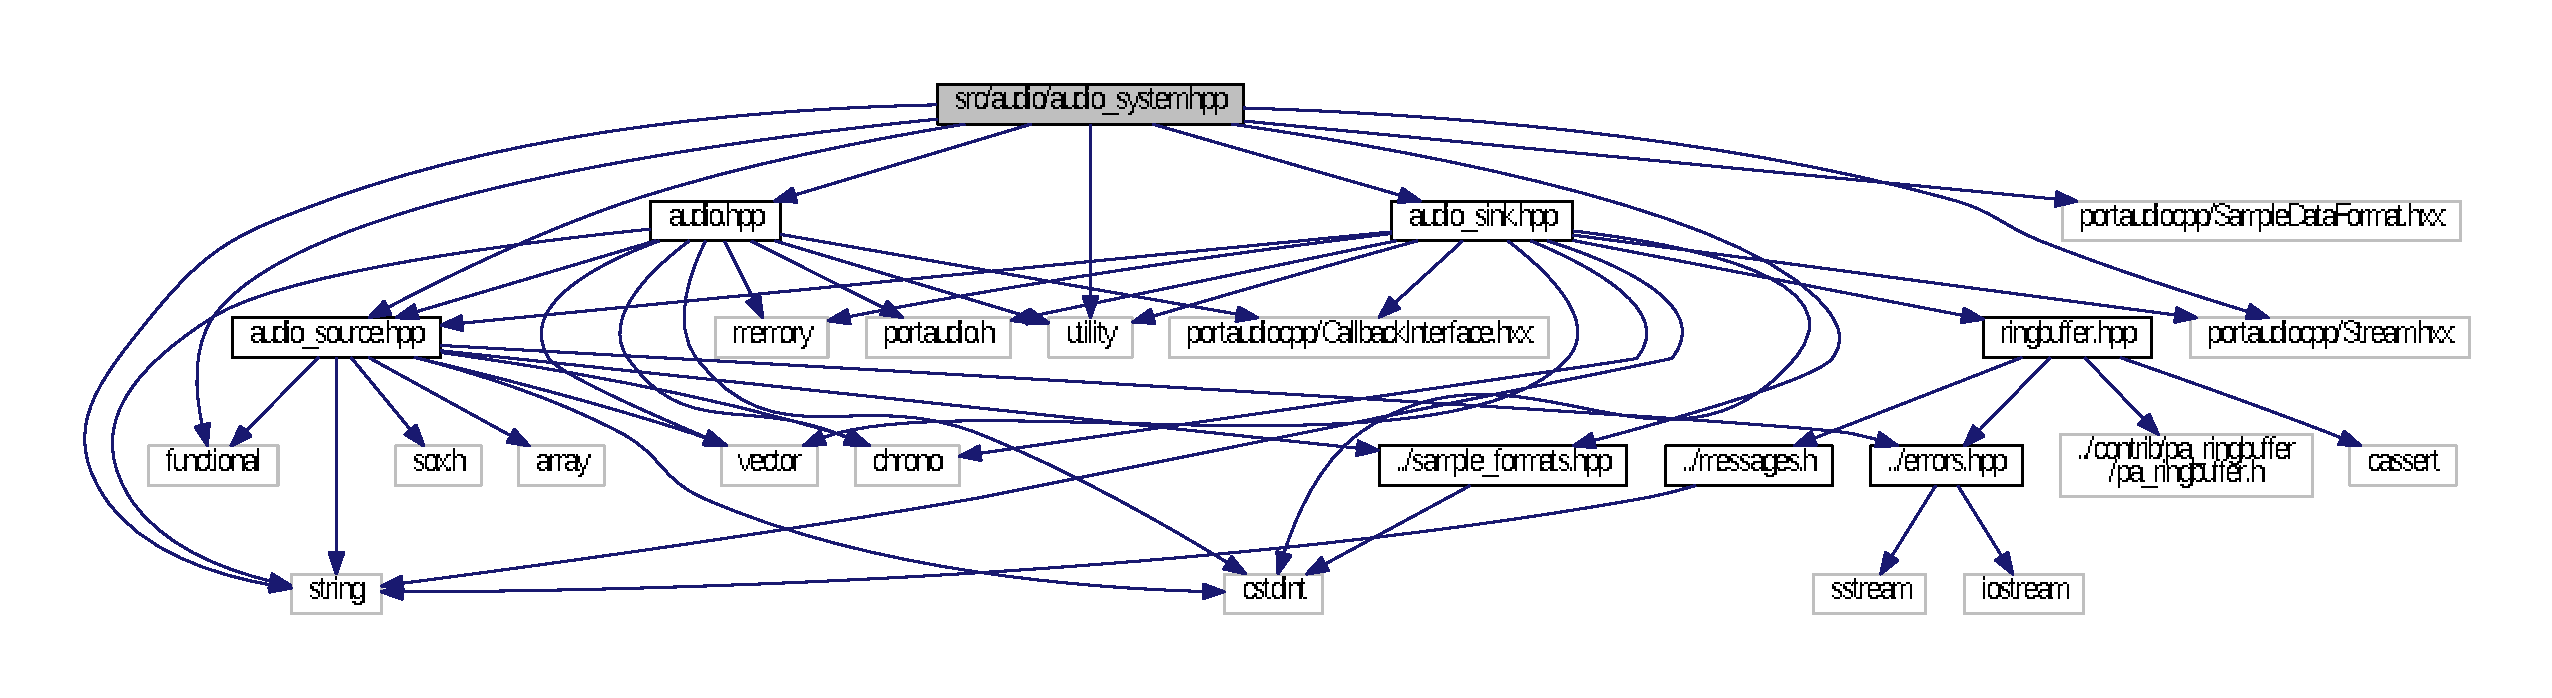
\includegraphics[width=350pt]{audio__system_8hpp__incl}
\end{center}
\end{figure}
This graph shows which files directly or indirectly include this file\+:
\nopagebreak
\begin{figure}[H]
\begin{center}
\leavevmode
\includegraphics[width=350pt]{audio__system_8hpp__dep__incl}
\end{center}
\end{figure}
\subsection*{Classes}
\begin{DoxyCompactItemize}
\item 
class \hyperlink{classAudioSystem}{Audio\+System}
\begin{DoxyCompactList}\small\item\em An \hyperlink{classAudioSystem}{Audio\+System} represents the entire audio stack used by playd. \end{DoxyCompactList}\end{DoxyCompactItemize}


\subsection{Detailed Description}
Declaration of the \hyperlink{classAudioSystem}{Audio\+System} class. 

\begin{DoxySeeAlso}{See also}
\hyperlink{audio__system_8cpp}{audio/audio\+\_\+system.\+cpp} 
\end{DoxySeeAlso}


Definition in file \hyperlink{audio__system_8hpp_source}{audio\+\_\+system.\+hpp}.


\hypertarget{audio__system_8hpp_source}{\section{audio\+\_\+system.\+hpp}
\label{audio__system_8hpp_source}\index{src/audio/audio\+\_\+system.\+hpp@{src/audio/audio\+\_\+system.\+hpp}}
}

\begin{DoxyCode}
00001 \textcolor{comment}{// This file is part of playd.}
00002 \textcolor{comment}{// playd is licenced under the MIT license: see LICENSE.txt.}
00003 
00010 \textcolor{preprocessor}{#ifndef PS\_AUDIO\_SYSTEM\_HPP}
00011 \textcolor{preprocessor}{#define PS\_AUDIO\_SYSTEM\_HPP}
00012 
00013 \textcolor{preprocessor}{#include <functional>}
00014 \textcolor{preprocessor}{#include <string>}
00015 \textcolor{preprocessor}{#include <utility>}
00016 
00017 \textcolor{preprocessor}{#include "portaudiocpp/SampleDataFormat.hxx"}
00018 \textcolor{preprocessor}{#include "portaudiocpp/Stream.hxx"}
00019 \textcolor{keyword}{namespace }portaudio \{
00020 \textcolor{keyword}{class }CallbackInterface;
00021 \textcolor{keyword}{class }Device;
00022 \}
00023 
00024 \textcolor{preprocessor}{#include "../sample\_formats.hpp"}
00025 \textcolor{preprocessor}{#include "\hyperlink{audio__sink_8hpp}{audio\_sink.hpp}"}
00026 \textcolor{preprocessor}{#include "\hyperlink{audio__source_8hpp}{audio\_source.hpp}"}
00027 \textcolor{preprocessor}{#include "\hyperlink{audio_8hpp}{audio.hpp}"}
00028 
\hypertarget{audio__system_8hpp_source_l00040}{}\hyperlink{classAudioSystem}{00040} \textcolor{keyword}{class }\hyperlink{classAudioSystem}{AudioSystem} \{
00041 \textcolor{keyword}{public}:
\hypertarget{audio__system_8hpp_source_l00043}{}\hyperlink{classAudioSystem_a33bfa767bca10a6ce71e72708c586c67}{00043}     \textcolor{keyword}{using} \hyperlink{classAudioSystem_a33bfa767bca10a6ce71e72708c586c67}{Device} = std::pair<int, std::string>;
00044 
00050     \hyperlink{classAudioSystem_ad17cde8deff07ef7d7d56be62df98739}{AudioSystem}();
00051 
00055     \hyperlink{classAudioSystem_a9ad830040ea5f68a6a63957c6f281055}{~AudioSystem}();
00056 
00062     \hyperlink{classAudio}{Audio} *\hyperlink{classAudioSystem_a2172608177d2bd54377bfc3c61cd117d}{Load}(\textcolor{keyword}{const} std::string &path) \textcolor{keyword}{const};
00063 
00068     \textcolor{keywordtype}{void} \hyperlink{classAudioSystem_ade3b400828991d02e36a0b61302d30d2}{SetDeviceID}(\textcolor{keywordtype}{int} \textcolor{keywordtype}{id});
00069 
00075     std::vector<AudioSystem::Device> \hyperlink{classAudioSystem_aa268faeb9243c18588631024958856e6}{GetDevicesInfo}();
00076 
00082     \textcolor{keywordtype}{bool} \hyperlink{classAudioSystem_a001cd82f854883b80b3ed7d35795581b}{IsOutputDevice}(\textcolor{keywordtype}{int} \textcolor{keywordtype}{id});
00083 
00095     portaudio::Stream *\hyperlink{classAudioSystem_a78e8754440e0a29f5fac9ca1cd79a109}{Configure}(std::uint8\_t channel\_count,
00096                                  \hyperlink{sample__formats_8hpp_a21cca244e782ff3acc8805fb73236772}{SampleFormat} sample\_format,
00097                                  \textcolor{keywordtype}{double} sample\_rate, \textcolor{keywordtype}{size\_t} buffer\_size,
00098                                  portaudio::CallbackInterface &cb) \textcolor{keyword}{const};
00099 
00100 \textcolor{keyword}{private}:
\hypertarget{audio__system_8hpp_source_l00101}{}\hyperlink{classAudioSystem_a3071e6d8643b3d0275ba63820e6e0072}{00101}     std::string \hyperlink{classAudioSystem_a3071e6d8643b3d0275ba63820e6e0072}{device\_id}; 
00102 
00108     \textcolor{keyword}{const} portaudio::Device &\hyperlink{classAudioSystem_a513a0de4748574e25cba443f28949a90}{PaDeviceFrom}(\textcolor{keyword}{const} std::string &id\_string)
00109                     \textcolor{keyword}{const};
00110 
00116     portaudio::SampleDataFormat \hyperlink{classAudioSystem_aac640b14ad80c2518539bcafe9f4b5ac}{PaSampleFormatFrom}(
      \hyperlink{sample__formats_8hpp_a21cca244e782ff3acc8805fb73236772}{SampleFormat} fmt) \textcolor{keyword}{const};
00117 \};
00118 
00119 \textcolor{preprocessor}{#endif // PS\_AUDIO\_SYSTEM\_HPP}
\end{DoxyCode}

\hypertarget{ringbuffer_8hpp}{\section{src/audio/ringbuffer.hpp File Reference}
\label{ringbuffer_8hpp}\index{src/audio/ringbuffer.\+hpp@{src/audio/ringbuffer.\+hpp}}
}


The \hyperlink{classRingBuffer}{Ring\+Buffer} class template.  


{\ttfamily \#include $<$cassert$>$}\\*
{\ttfamily \#include \char`\"{}../contrib/pa\+\_\+ringbuffer/pa\+\_\+ringbuffer.\+h\char`\"{}}\\*
{\ttfamily \#include \char`\"{}../errors.\+hpp\char`\"{}}\\*
{\ttfamily \#include \char`\"{}../messages.\+h\char`\"{}}\\*
Include dependency graph for ringbuffer.\+hpp\+:
\nopagebreak
\begin{figure}[H]
\begin{center}
\leavevmode
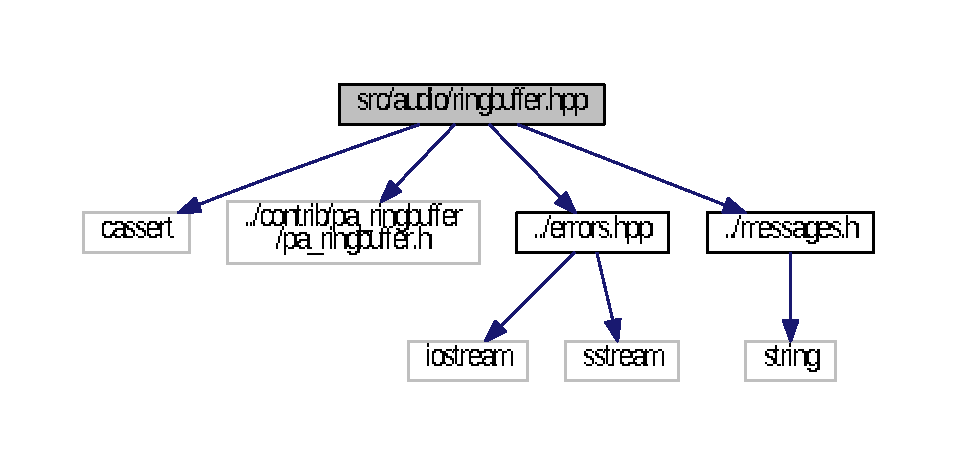
\includegraphics[width=350pt]{ringbuffer_8hpp__incl}
\end{center}
\end{figure}
This graph shows which files directly or indirectly include this file\+:
\nopagebreak
\begin{figure}[H]
\begin{center}
\leavevmode
\includegraphics[width=350pt]{ringbuffer_8hpp__dep__incl}
\end{center}
\end{figure}
\subsection*{Classes}
\begin{DoxyCompactItemize}
\item 
class \hyperlink{classRingBuffer}{Ring\+Buffer$<$ Rep\+T, Sample\+Count\+T $>$}
\begin{DoxyCompactList}\small\item\em A ring buffer. \end{DoxyCompactList}\end{DoxyCompactItemize}


\subsection{Detailed Description}
The \hyperlink{classRingBuffer}{Ring\+Buffer} class template. 



Definition in file \hyperlink{ringbuffer_8hpp_source}{ringbuffer.\+hpp}.


\hypertarget{ringbuffer_8hpp_source}{\section{ringbuffer.\+hpp}
\label{ringbuffer_8hpp_source}\index{src/audio/ringbuffer.\+hpp@{src/audio/ringbuffer.\+hpp}}
}

\begin{DoxyCode}
00001 \textcolor{comment}{// This file is part of playd.}
00002 \textcolor{comment}{// playd is licenced under the MIT license: see LICENSE.txt.}
00003 
00009 \textcolor{preprocessor}{#ifndef PS\_RINGBUFFER\_HPP}
00010 \textcolor{preprocessor}{#define PS\_RINGBUFFER\_HPP}
00011 
00012 \textcolor{preprocessor}{#include <cassert>}
00013 
00014 \textcolor{keyword}{extern} \textcolor{stringliteral}{"C"} \{
00015 \textcolor{preprocessor}{#include "../contrib/pa\_ringbuffer/pa\_ringbuffer.h"}
00016 \}
00017 
00018 \textcolor{preprocessor}{#include "../errors.hpp"}
00019 \textcolor{preprocessor}{#include "../messages.h"}
00020 
00029 \textcolor{keyword}{template} <\textcolor{keyword}{typename} RepT, \textcolor{keyword}{typename} SampleCountT>
\hypertarget{ringbuffer_8hpp_source_l00030}{}\hyperlink{classRingBuffer}{00030} \textcolor{keyword}{class }\hyperlink{classRingBuffer}{RingBuffer} \{
00031 \textcolor{keyword}{public}:
\hypertarget{ringbuffer_8hpp_source_l00042}{}\hyperlink{classRingBuffer_a2f831ec4941885db960a833cb807465e}{00042}     \hyperlink{classRingBuffer_a2f831ec4941885db960a833cb807465e}{RingBuffer}(\textcolor{keywordtype}{int} power, \textcolor{keywordtype}{int} size)
00043     \{
00044         assert(0 < power);
00045         assert(0 < size);
00046 
00047         this->\hyperlink{classRingBuffer_a10985ec171bcc15c1301dc74fcb6e7b2}{rb} = \textcolor{keyword}{new} PaUtilRingBuffer;
00048         this->\hyperlink{classRingBuffer_a09103853af3302b27d2bbd46f1dfbe87}{buffer} = \textcolor{keyword}{new} \textcolor{keywordtype}{char}[(1 << power) * size];
00049 
00050         \textcolor{keywordtype}{int} init\_result = PaUtil\_InitializeRingBuffer(
00051                         this->\hyperlink{classRingBuffer_a10985ec171bcc15c1301dc74fcb6e7b2}{rb}, size,
00052                         static\_cast<ring\_buffer\_size\_t>(1 << power),
00053                         this->\hyperlink{classRingBuffer_a09103853af3302b27d2bbd46f1dfbe87}{buffer});
00054         \textcolor{keywordflow}{if} (init\_result != 0) \{
00055             \textcolor{keywordflow}{throw} \textcolor{keyword}{new} \hyperlink{classInternalError}{InternalError}(\hyperlink{messages_8h_a3bf0477dded19418d7ecac95aeae8856}{MSG\_OUTPUT\_RINGINIT});
00056         \}
00057 
00058         assert(this->\hyperlink{classRingBuffer_a10985ec171bcc15c1301dc74fcb6e7b2}{rb} != \textcolor{keyword}{nullptr});
00059         assert(this->\hyperlink{classRingBuffer_a09103853af3302b27d2bbd46f1dfbe87}{buffer} != \textcolor{keyword}{nullptr});
00060     \}
00061 
\hypertarget{ringbuffer_8hpp_source_l00063}{}\hyperlink{classRingBuffer_a39d93b7f608eb69a7a569e61b5abc979}{00063}     \hyperlink{classRingBuffer_a39d93b7f608eb69a7a569e61b5abc979}{~RingBuffer}()
00064     \{
00065         assert(this->\hyperlink{classRingBuffer_a10985ec171bcc15c1301dc74fcb6e7b2}{rb} != \textcolor{keyword}{nullptr});
00066         \textcolor{keyword}{delete} this->\hyperlink{classRingBuffer_a10985ec171bcc15c1301dc74fcb6e7b2}{rb};
00067 
00068         assert(this->\hyperlink{classRingBuffer_a09103853af3302b27d2bbd46f1dfbe87}{buffer} != \textcolor{keyword}{nullptr});
00069         \textcolor{keyword}{delete}[] this->\hyperlink{classRingBuffer_a09103853af3302b27d2bbd46f1dfbe87}{buffer};
00070     \}
00071 
00073     \hyperlink{classRingBuffer_a2f831ec4941885db960a833cb807465e}{RingBuffer}(\textcolor{keyword}{const} \hyperlink{classRingBuffer}{RingBuffer} &) = \textcolor{keyword}{delete};
00074 
00076     \hyperlink{classRingBuffer}{RingBuffer} &\hyperlink{classRingBuffer_a6f552e291e577aeffc57b846969d11d6}{operator=}(\textcolor{keyword}{const} \hyperlink{classRingBuffer}{RingBuffer} &) = \textcolor{keyword}{delete};
00077 
\hypertarget{ringbuffer_8hpp_source_l00083}{}\hyperlink{classRingBuffer_ab00617ab6e379ad146cb7b80079f4c4c}{00083}     SampleCountT \hyperlink{classRingBuffer_ab00617ab6e379ad146cb7b80079f4c4c}{WriteCapacity}()\textcolor{keyword}{ const}
00084 \textcolor{keyword}{    }\{
00085         \textcolor{keywordflow}{return} \hyperlink{classRingBuffer_ae907c82ba714a087d9f35b089f9fbf77}{CountCast}(PaUtil\_GetRingBufferWriteAvailable(this->\hyperlink{classRingBuffer_a10985ec171bcc15c1301dc74fcb6e7b2}{rb}));
00086     \}
00087 
\hypertarget{ringbuffer_8hpp_source_l00093}{}\hyperlink{classRingBuffer_a7086cc66306105db205842af7a88c2d8}{00093}     SampleCountT \hyperlink{classRingBuffer_a7086cc66306105db205842af7a88c2d8}{ReadCapacity}()\textcolor{keyword}{ const}
00094 \textcolor{keyword}{    }\{
00095         \textcolor{keywordflow}{return} \hyperlink{classRingBuffer_ae907c82ba714a087d9f35b089f9fbf77}{CountCast}(PaUtil\_GetRingBufferReadAvailable(this->\hyperlink{classRingBuffer_a10985ec171bcc15c1301dc74fcb6e7b2}{rb}));
00096     \}
00097 
\hypertarget{ringbuffer_8hpp_source_l00120}{}\hyperlink{classRingBuffer_aa7f863968cb641946b0cf341bda11e16}{00120}     SampleCountT \hyperlink{classRingBuffer_aa7f863968cb641946b0cf341bda11e16}{Write}(RepT *start, SampleCountT count)
00121     \{
00122         assert(0 < count);
00123         assert(count <= \hyperlink{classRingBuffer_ab00617ab6e379ad146cb7b80079f4c4c}{WriteCapacity}());
00124 
00125         \textcolor{keywordflow}{return} \hyperlink{classRingBuffer_ae907c82ba714a087d9f35b089f9fbf77}{CountCast}(PaUtil\_WriteRingBuffer(
00126                         this->\hyperlink{classRingBuffer_a10985ec171bcc15c1301dc74fcb6e7b2}{rb}, start,
00127                         static\_cast<ring\_buffer\_size\_t>(count)));
00128     \}
00129 
\hypertarget{ringbuffer_8hpp_source_l00149}{}\hyperlink{classRingBuffer_af892330ee102bd50a493b8afa814a0f0}{00149}     SampleCountT \hyperlink{classRingBuffer_af892330ee102bd50a493b8afa814a0f0}{Read}(RepT *start, SampleCountT count)
00150     \{
00151         assert(0 < count);
00152         assert(count <= \hyperlink{classRingBuffer_a7086cc66306105db205842af7a88c2d8}{ReadCapacity}());
00153 
00154         \textcolor{keywordflow}{return} \hyperlink{classRingBuffer_ae907c82ba714a087d9f35b089f9fbf77}{CountCast}(PaUtil\_ReadRingBuffer(
00155                         this->\hyperlink{classRingBuffer_a10985ec171bcc15c1301dc74fcb6e7b2}{rb}, start,
00156                         static\_cast<ring\_buffer\_size\_t>(count)));
00157     \}
00158 
\hypertarget{ringbuffer_8hpp_source_l00160}{}\hyperlink{classRingBuffer_a1eb1acca6905e7678fbbdb70238cdc26}{00160}     \textcolor{keywordtype}{void} \hyperlink{classRingBuffer_a1eb1acca6905e7678fbbdb70238cdc26}{Flush}()
00161     \{
00162         PaUtil\_FlushRingBuffer(this->\hyperlink{classRingBuffer_a10985ec171bcc15c1301dc74fcb6e7b2}{rb});
00163     \}
00164 
00165 \textcolor{keyword}{private}:
\hypertarget{ringbuffer_8hpp_source_l00166}{}\hyperlink{classRingBuffer_a09103853af3302b27d2bbd46f1dfbe87}{00166}     \textcolor{keywordtype}{char} *\hyperlink{classRingBuffer_a09103853af3302b27d2bbd46f1dfbe87}{buffer};         
\hypertarget{ringbuffer_8hpp_source_l00167}{}\hyperlink{classRingBuffer_a10985ec171bcc15c1301dc74fcb6e7b2}{00167}     PaUtilRingBuffer *\hyperlink{classRingBuffer_a10985ec171bcc15c1301dc74fcb6e7b2}{rb}; 
00168 
\hypertarget{ringbuffer_8hpp_source_l00174}{}\hyperlink{classRingBuffer_ae907c82ba714a087d9f35b089f9fbf77}{00174}     SampleCountT \hyperlink{classRingBuffer_ae907c82ba714a087d9f35b089f9fbf77}{CountCast}(ring\_buffer\_size\_t count)\textcolor{keyword}{ const}
00175 \textcolor{keyword}{    }\{
00176         \textcolor{keywordflow}{return} \textcolor{keyword}{static\_cast<}SampleCountT\textcolor{keyword}{>}(count);
00177     \}
00178 \};
00179 
00180 \textcolor{preprocessor}{#endif // PS\_RINGBUFFER\_HPP}
\end{DoxyCode}

\hypertarget{cmd_8cpp}{\section{src/cmd.cpp File Reference}
\label{cmd_8cpp}\index{src/cmd.\+cpp@{src/cmd.\+cpp}}
}


Implementation of the \hyperlink{classCommandHandler}{Command\+Handler} class.  


{\ttfamily \#include $<$iostream$>$}\\*
{\ttfamily \#include $<$string$>$}\\*
{\ttfamily \#include \char`\"{}cmd.\+hpp\char`\"{}}\\*
{\ttfamily \#include \char`\"{}errors.\+hpp\char`\"{}}\\*
{\ttfamily \#include \char`\"{}io/io\+\_\+response.\+hpp\char`\"{}}\\*
{\ttfamily \#include \char`\"{}messages.\+h\char`\"{}}\\*
Include dependency graph for cmd.\+cpp\+:
\nopagebreak
\begin{figure}[H]
\begin{center}
\leavevmode
\includegraphics[width=350pt]{cmd_8cpp__incl}
\end{center}
\end{figure}


\subsection{Detailed Description}
Implementation of the \hyperlink{classCommandHandler}{Command\+Handler} class. 

\begin{DoxySeeAlso}{See also}
\hyperlink{cmd_8hpp}{cmd.\+hpp} 
\end{DoxySeeAlso}


Definition in file \hyperlink{cmd_8cpp_source}{cmd.\+cpp}.


\hypertarget{cmd_8cpp_source}{\section{cmd.\+cpp}
\label{cmd_8cpp_source}\index{src/cmd.\+cpp@{src/cmd.\+cpp}}
}

\begin{DoxyCode}
00001 \textcolor{comment}{// This file is part of playd.}
00002 \textcolor{comment}{// playd is licenced under the MIT license: see LICENSE.txt.}
00003 
00010 \textcolor{preprocessor}{#include <iostream>}
00011 \textcolor{preprocessor}{#include <string>}
00012 
00013 \textcolor{preprocessor}{#include "\hyperlink{cmd_8hpp}{cmd.hpp}"}
00014 \textcolor{preprocessor}{#include "\hyperlink{errors_8hpp}{errors.hpp}"}
00015 \textcolor{preprocessor}{#include "\hyperlink{io__response_8hpp}{io/io\_response.hpp}"}
00016 \textcolor{preprocessor}{#include "\hyperlink{messages_8h}{messages.h}"}
00017 
\hypertarget{cmd_8cpp_source_l00018}{}\hyperlink{classCommandHandler_ae4d47b90e2cf2ab6d514576fedeb2192}{00018} \hyperlink{classCommandHandler_ae4d47b90e2cf2ab6d514576fedeb2192}{CommandHandler::CommandHandler}(\hyperlink{classPlayer}{Player} &player) : player(player)
00019 \{
00020 \}
00021 
\hypertarget{cmd_8cpp_source_l00022}{}\hyperlink{classCommandHandler_abc1ad0dfbff50db168d0a65cf05b169e}{00022} \textcolor{keywordtype}{bool} \hyperlink{classCommandHandler_abc1ad0dfbff50db168d0a65cf05b169e}{CommandHandler::Handle}(\textcolor{keyword}{const} \hyperlink{classCommandHandler_ae6cc650f171966041b385c8a4a766639}{CommandHandler::WordList} &
      words)
00023 \{
00024     \textcolor{keywordflow}{if} (words.size() == 1) \{
00025         \textcolor{keywordflow}{return} \hyperlink{classCommandHandler_a22ac65683643c6f6037441a8e5fd04d4}{RunNullary}(words[0]);
00026     \} \textcolor{keywordflow}{else} \textcolor{keywordflow}{if} (words.size() == 2 && !words[1].empty()) \{
00027         \textcolor{keywordflow}{return} \hyperlink{classCommandHandler_a75904aa3532bba1e548fbcff00544d46}{RunUnary}(words[0], words[1]);
00028     \}
00029     \textcolor{keywordflow}{return} \textcolor{keyword}{false};
00030 \}
00031 
\hypertarget{cmd_8cpp_source_l00032}{}\hyperlink{classCommandHandler_a22ac65683643c6f6037441a8e5fd04d4}{00032} \textcolor{keywordtype}{bool} \hyperlink{classCommandHandler_a22ac65683643c6f6037441a8e5fd04d4}{CommandHandler::RunNullary}(\textcolor{keyword}{const} std::string &cmd)
00033 \{
00034     \textcolor{keywordflow}{if} (\textcolor{stringliteral}{"play"} == cmd) \textcolor{keywordflow}{return} this->\hyperlink{classCommandHandler_a398ba97a0625f5fbc3ced6679cfd3766}{player}.\hyperlink{classPlayer_a1df3950102f682608482042cdea96598}{Play}();
00035     \textcolor{keywordflow}{if} (\textcolor{stringliteral}{"stop"} == cmd) \textcolor{keywordflow}{return} this->\hyperlink{classCommandHandler_a398ba97a0625f5fbc3ced6679cfd3766}{player}.\hyperlink{classPlayer_abe074115b0ffa631ea432a1b84171599}{Stop}();
00036     \textcolor{keywordflow}{if} (\textcolor{stringliteral}{"eject"} == cmd) \textcolor{keywordflow}{return} this->\hyperlink{classCommandHandler_a398ba97a0625f5fbc3ced6679cfd3766}{player}.\hyperlink{classPlayer_ac93a5310c751e8a9221780933f7a9dd6}{Eject}();
00037     \textcolor{keywordflow}{if} (\textcolor{stringliteral}{"quit"} == cmd) \textcolor{keywordflow}{return} this->\hyperlink{classCommandHandler_a398ba97a0625f5fbc3ced6679cfd3766}{player}.\hyperlink{classPlayer_a7d5c0535d543b358b6deecb054565b97}{Quit}();
00038     \textcolor{keywordflow}{return} \textcolor{keyword}{false};
00039 \}
00040 
\hypertarget{cmd_8cpp_source_l00041}{}\hyperlink{classCommandHandler_a75904aa3532bba1e548fbcff00544d46}{00041} \textcolor{keywordtype}{bool} \hyperlink{classCommandHandler_a75904aa3532bba1e548fbcff00544d46}{CommandHandler::RunUnary}(\textcolor{keyword}{const} std::string &cmd, \textcolor{keyword}{const} std::string &arg)
00042 \{
00043     \textcolor{keywordflow}{if} (\textcolor{stringliteral}{"load"} == cmd) \textcolor{keywordflow}{return} this->\hyperlink{classCommandHandler_a398ba97a0625f5fbc3ced6679cfd3766}{player}.\hyperlink{classPlayer_a41c5eccb1f3b86383eaafe56a40a60e0}{Load}(arg);
00044     \textcolor{keywordflow}{if} (\textcolor{stringliteral}{"seek"} == cmd) \textcolor{keywordflow}{return} this->\hyperlink{classCommandHandler_a398ba97a0625f5fbc3ced6679cfd3766}{player}.\hyperlink{classPlayer_a873c7e0a5be71efbadeebfbc20d7448a}{Seek}(arg);
00045     \textcolor{keywordflow}{return} \textcolor{keyword}{false};
00046 \}
\end{DoxyCode}

\hypertarget{cmd_8hpp}{\section{src/cmd.hpp File Reference}
\label{cmd_8hpp}\index{src/cmd.\+hpp@{src/cmd.\+hpp}}
}


Declaration of the \hyperlink{classCommandHandler}{Command\+Handler} class.  


{\ttfamily \#include $<$functional$>$}\\*
{\ttfamily \#include $<$map$>$}\\*
{\ttfamily \#include $<$memory$>$}\\*
{\ttfamily \#include $<$vector$>$}\\*
{\ttfamily \#include \char`\"{}player/player.\+hpp\char`\"{}}\\*
Include dependency graph for cmd.\+hpp\+:
\nopagebreak
\begin{figure}[H]
\begin{center}
\leavevmode
\includegraphics[width=350pt]{cmd_8hpp__incl}
\end{center}
\end{figure}
This graph shows which files directly or indirectly include this file\+:
\nopagebreak
\begin{figure}[H]
\begin{center}
\leavevmode
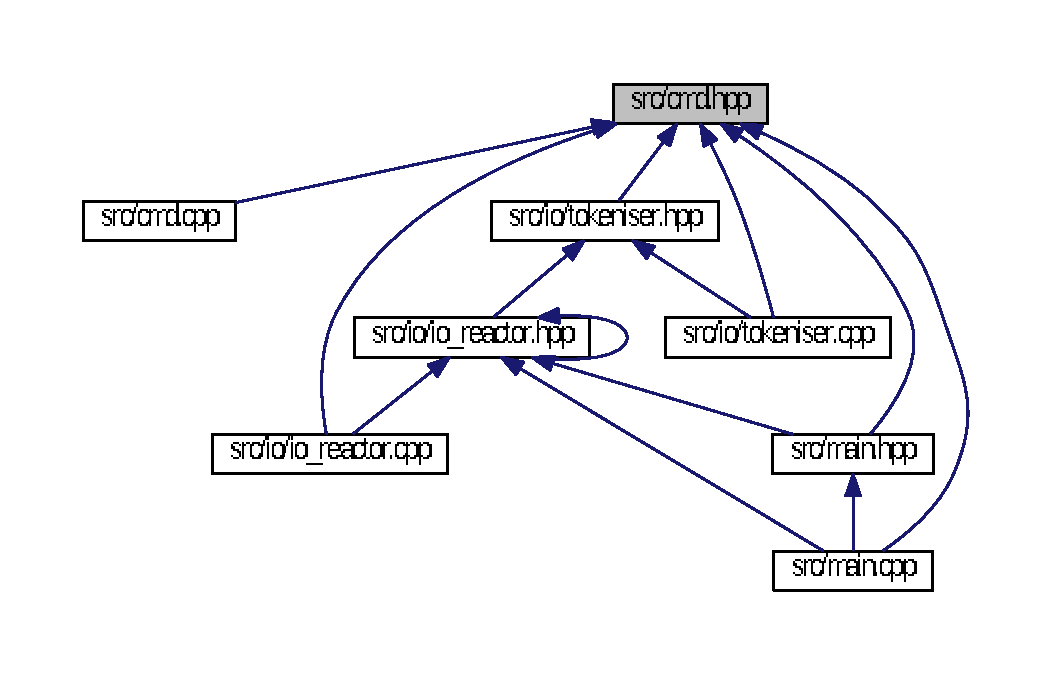
\includegraphics[width=350pt]{cmd_8hpp__dep__incl}
\end{center}
\end{figure}
\subsection*{Classes}
\begin{DoxyCompactItemize}
\item 
class \hyperlink{classCommandHandler}{Command\+Handler}
\begin{DoxyCompactList}\small\item\em The playd command handler. \end{DoxyCompactList}\end{DoxyCompactItemize}


\subsection{Detailed Description}
Declaration of the \hyperlink{classCommandHandler}{Command\+Handler} class. 

\begin{DoxySeeAlso}{See also}
\hyperlink{cmd_8cpp}{cmd.\+cpp} 
\end{DoxySeeAlso}


Definition in file \hyperlink{cmd_8hpp_source}{cmd.\+hpp}.


\hypertarget{cmd_8hpp_source}{\section{cmd.\+hpp}
\label{cmd_8hpp_source}\index{src/cmd.\+hpp@{src/cmd.\+hpp}}
}

\begin{DoxyCode}
00001 \textcolor{comment}{// This file is part of playd.}
00002 \textcolor{comment}{// playd is licenced under the MIT license: see LICENSE.txt.}
00003 
00010 \textcolor{preprocessor}{#ifndef PS\_CMD\_HPP}
00011 \textcolor{preprocessor}{#define PS\_CMD\_HPP}
00012 
00013 \textcolor{preprocessor}{#include <functional>}
00014 \textcolor{preprocessor}{#include <map>}
00015 \textcolor{preprocessor}{#include <memory>}
00016 \textcolor{preprocessor}{#include <vector>}
00017 
00018 \textcolor{preprocessor}{#include "\hyperlink{player_8hpp}{player/player.hpp}"}
00019 
00020 \textcolor{preprocessor}{#ifdef IGNORE}
00021 \textcolor{preprocessor}{#undef IGNORE}
00022 \textcolor{preprocessor}{#endif}
00023 
\hypertarget{cmd_8hpp_source_l00027}{}\hyperlink{classCommandHandler}{00027} \textcolor{keyword}{class }\hyperlink{classCommandHandler}{CommandHandler} \{
00028 \textcolor{keyword}{public}:
\hypertarget{cmd_8hpp_source_l00030}{}\hyperlink{classCommandHandler_ae6cc650f171966041b385c8a4a766639}{00030}     \textcolor{keyword}{using} \hyperlink{classCommandHandler_ae6cc650f171966041b385c8a4a766639}{WordList} = std::vector<std::string>;
00031 
00037     \hyperlink{classCommandHandler_ae4d47b90e2cf2ab6d514576fedeb2192}{CommandHandler}(\hyperlink{classPlayer}{Player} &\hyperlink{classCommandHandler_a398ba97a0625f5fbc3ced6679cfd3766}{player});
00038 
00044     \textcolor{keywordtype}{bool} \hyperlink{classCommandHandler_abc1ad0dfbff50db168d0a65cf05b169e}{Handle}(\textcolor{keyword}{const} \hyperlink{classCommandHandler_ae6cc650f171966041b385c8a4a766639}{WordList} &words);
00045 
00046 \textcolor{keyword}{private}:
\hypertarget{cmd_8hpp_source_l00048}{}\hyperlink{classCommandHandler_a398ba97a0625f5fbc3ced6679cfd3766}{00048}     \hyperlink{classPlayer}{Player} &\hyperlink{classCommandHandler_a398ba97a0625f5fbc3ced6679cfd3766}{player};
00049 
00057     \textcolor{keywordtype}{bool} \hyperlink{classCommandHandler_a22ac65683643c6f6037441a8e5fd04d4}{RunNullary}(\textcolor{keyword}{const} std::string &cmd);
00058 
00067     \textcolor{keywordtype}{bool} \hyperlink{classCommandHandler_a75904aa3532bba1e548fbcff00544d46}{RunUnary}(\textcolor{keyword}{const} std::string &cmd, \textcolor{keyword}{const} std::string &arg);
00068 \};
00069 
00070 \textcolor{preprocessor}{#endif // PS\_CMD\_HPP}
\end{DoxyCode}

\hypertarget{errors_8cpp}{\section{src/errors.cpp File Reference}
\label{errors_8cpp}\index{src/errors.\+cpp@{src/errors.\+cpp}}
}


Implementation of the playd \hyperlink{classError}{Error} exception set.  


{\ttfamily \#include \char`\"{}errors.\+hpp\char`\"{}}\\*
Include dependency graph for errors.\+cpp\+:
\nopagebreak
\begin{figure}[H]
\begin{center}
\leavevmode
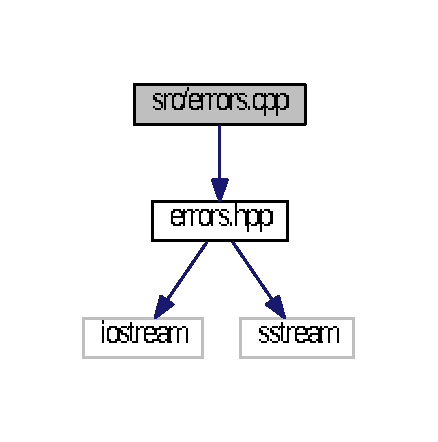
\includegraphics[width=210pt]{errors_8cpp__incl}
\end{center}
\end{figure}


\subsection{Detailed Description}
Implementation of the playd \hyperlink{classError}{Error} exception set. 

\begin{DoxySeeAlso}{See also}
\hyperlink{errors_8hpp}{errors.\+hpp} 
\end{DoxySeeAlso}


Definition in file \hyperlink{errors_8cpp_source}{errors.\+cpp}.


\hypertarget{errors_8cpp_source}{\section{errors.\+cpp}
\label{errors_8cpp_source}\index{src/errors.\+cpp@{src/errors.\+cpp}}
}

\begin{DoxyCode}
00001 \textcolor{comment}{// This file is part of playd.}
00002 \textcolor{comment}{// playd is licenced under the MIT license: see LICENSE.txt.}
00003 
00010 \textcolor{preprocessor}{#include "\hyperlink{errors_8hpp}{errors.hpp}"}
00011 
\hypertarget{errors_8cpp_source_l00012}{}\hyperlink{classError_accd611f3ddae0828adeb6ca251113ffd}{00012} \hyperlink{classError_accd611f3ddae0828adeb6ca251113ffd}{Error::Error}(\textcolor{keyword}{const} std::string &message)
00013 \{
00014     this->message = std::string(message);
00015 \}
00016 
\hypertarget{errors_8cpp_source_l00017}{}\hyperlink{classError_a006605b13a346cf019f60420f1b29b5a}{00017} \textcolor{keyword}{const} std::string &\hyperlink{classError_a006605b13a346cf019f60420f1b29b5a}{Error::Message}()\textcolor{keyword}{ const}
00018 \textcolor{keyword}{}\{
00019     \textcolor{keywordflow}{return} this->\hyperlink{classError_aa4713ef3ee9c3c0da43a54b01949510d}{message};
00020 \}
\end{DoxyCode}

\hypertarget{errors_8hpp}{\section{src/errors.hpp File Reference}
\label{errors_8hpp}\index{src/errors.\+hpp@{src/errors.\+hpp}}
}


Declarations of the playd \hyperlink{classError}{Error} exception set.  


{\ttfamily \#include $<$iostream$>$}\\*
{\ttfamily \#include $<$sstream$>$}\\*
Include dependency graph for errors.\+hpp\+:
\nopagebreak
\begin{figure}[H]
\begin{center}
\leavevmode
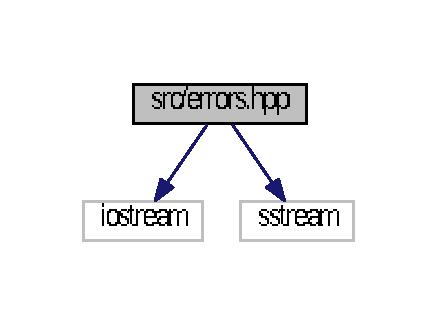
\includegraphics[width=210pt]{errors_8hpp__incl}
\end{center}
\end{figure}
This graph shows which files directly or indirectly include this file\+:
\nopagebreak
\begin{figure}[H]
\begin{center}
\leavevmode
\includegraphics[width=350pt]{errors_8hpp__dep__incl}
\end{center}
\end{figure}
\subsection*{Classes}
\begin{DoxyCompactItemize}
\item 
class \hyperlink{classError}{Error}
\begin{DoxyCompactList}\small\item\em A playd exception. \end{DoxyCompactList}\item 
class \hyperlink{classConfigError}{Config\+Error}
\begin{DoxyCompactList}\small\item\em An \hyperlink{classError}{Error} signifying that playd has been improperly configured. \end{DoxyCompactList}\item 
class \hyperlink{classInternalError}{Internal\+Error}
\begin{DoxyCompactList}\small\item\em An \hyperlink{classError}{Error} signifying that playd has hit an internal snag. \end{DoxyCompactList}\item 
class \hyperlink{classFileError}{File\+Error}
\begin{DoxyCompactList}\small\item\em An \hyperlink{classError}{Error} signifying that playd can't read a file. \end{DoxyCompactList}\item 
class \hyperlink{classDebug}{Debug}
\begin{DoxyCompactList}\small\item\em Class for telling the human what playd is doing. \end{DoxyCompactList}\end{DoxyCompactItemize}


\subsection{Detailed Description}
Declarations of the playd \hyperlink{classError}{Error} exception set. 

\begin{DoxySeeAlso}{See also}
\hyperlink{errors_8cpp}{errors.\+cpp} 
\end{DoxySeeAlso}


Definition in file \hyperlink{errors_8hpp_source}{errors.\+hpp}.


\hypertarget{errors_8hpp_source}{\section{errors.\+hpp}
\label{errors_8hpp_source}\index{src/errors.\+hpp@{src/errors.\+hpp}}
}

\begin{DoxyCode}
00001 \textcolor{comment}{// This file is part of playd.}
00002 \textcolor{comment}{// playd is licenced under the MIT license: see LICENSE.txt.}
00003 
00010 \textcolor{preprocessor}{#ifndef PS\_ERRORS\_HPP}
00011 \textcolor{preprocessor}{#define PS\_ERRORS\_HPP}
00012 
00013 \textcolor{preprocessor}{#include <iostream>}
00014 \textcolor{preprocessor}{#include <sstream>}
00015 
\hypertarget{errors_8hpp_source_l00019}{}\hyperlink{classError}{00019} \textcolor{keyword}{class }\hyperlink{classError}{Error} \{
00020 \textcolor{keyword}{public}:
00025     \hyperlink{classError_accd611f3ddae0828adeb6ca251113ffd}{Error}(\textcolor{keyword}{const} std::string &\hyperlink{classError_aa4713ef3ee9c3c0da43a54b01949510d}{message});
00026 
00031     \textcolor{keyword}{const} std::string &\hyperlink{classError_a006605b13a346cf019f60420f1b29b5a}{Message}() \textcolor{keyword}{const};
00032 
00033 \textcolor{keyword}{private}:
\hypertarget{errors_8hpp_source_l00034}{}\hyperlink{classError_aa4713ef3ee9c3c0da43a54b01949510d}{00034}     std::string \hyperlink{classError_aa4713ef3ee9c3c0da43a54b01949510d}{message}; 
00035 \};
00036 
00037 \textcolor{comment}{//}
00038 \textcolor{comment}{// Error sub-categories}
00039 \textcolor{comment}{//}
00040 
\hypertarget{errors_8hpp_source_l00044}{}\hyperlink{classConfigError}{00044} \textcolor{keyword}{class }\hyperlink{classConfigError}{ConfigError} : \textcolor{keyword}{public} \hyperlink{classError}{Error} \{
00045 \textcolor{keyword}{public}:
\hypertarget{errors_8hpp_source_l00050}{}\hyperlink{classConfigError_a0df38d0770d8e8299e628793058bb2eb}{00050}     \hyperlink{classConfigError_a0df38d0770d8e8299e628793058bb2eb}{ConfigError}(\textcolor{keyword}{const} std::string &\hyperlink{classError_aa4713ef3ee9c3c0da43a54b01949510d}{message}) : \hyperlink{classError}{Error}(message) \{\};
00051 \};
00052 
\hypertarget{errors_8hpp_source_l00056}{}\hyperlink{classInternalError}{00056} \textcolor{keyword}{class }\hyperlink{classInternalError}{InternalError} : \textcolor{keyword}{public} \hyperlink{classError}{Error} \{
00057 \textcolor{keyword}{public}:
\hypertarget{errors_8hpp_source_l00062}{}\hyperlink{classInternalError_a02889f0d60c52bb6b92c522c034aa0bf}{00062}     \hyperlink{classInternalError_a02889f0d60c52bb6b92c522c034aa0bf}{InternalError}(\textcolor{keyword}{const} std::string &\hyperlink{classError_aa4713ef3ee9c3c0da43a54b01949510d}{message}) : \hyperlink{classError}{Error}(message) \{\};
00063 \};
00064 
\hypertarget{errors_8hpp_source_l00068}{}\hyperlink{classFileError}{00068} \textcolor{keyword}{class }\hyperlink{classFileError}{FileError} : \textcolor{keyword}{public} \hyperlink{classError}{Error} \{
00069 \textcolor{keyword}{public}:
\hypertarget{errors_8hpp_source_l00074}{}\hyperlink{classFileError_a3daf79a4497298aa7d8dbd42897074d2}{00074}     \hyperlink{classFileError_a3daf79a4497298aa7d8dbd42897074d2}{FileError}(\textcolor{keyword}{const} std::string &\hyperlink{classError_aa4713ef3ee9c3c0da43a54b01949510d}{message}) : \hyperlink{classError}{Error}(message) \{\};
00075 \};
00076 
\hypertarget{errors_8hpp_source_l00078}{}\hyperlink{classDebug}{00078} \textcolor{keyword}{class }\hyperlink{classDebug}{Debug} \{
00079 \textcolor{keyword}{public}:
\hypertarget{errors_8hpp_source_l00081}{}\hyperlink{classDebug_a5b453c195c4cfffed2702c3330f53a64}{00081}     \textcolor{keyword}{inline} \hyperlink{classDebug_a5b453c195c4cfffed2702c3330f53a64}{Debug}()
00082     \{
00083         \hyperlink{classDebug_a45f5726114c0078b31b9a0f70199f51e}{oss} << \textcolor{stringliteral}{"DEBUG:"};
00084     \}
00085 
\hypertarget{errors_8hpp_source_l00087}{}\hyperlink{classDebug_a911a84a0f56b770724e09a049399dc30}{00087}     \textcolor{keyword}{inline} \hyperlink{classDebug_a911a84a0f56b770724e09a049399dc30}{~Debug}()
00088     \{
00089         std::cerr << \hyperlink{classDebug_a45f5726114c0078b31b9a0f70199f51e}{oss}.str();
00090     \}
00091 
00098     \textcolor{keyword}{template} <\textcolor{keyword}{typename} T>
\hypertarget{errors_8hpp_source_l00099}{}\hyperlink{classDebug_a7fdf38b9c8d1976b5a723e4bf59fec49}{00099}     \textcolor{keyword}{inline} \hyperlink{classDebug}{Debug} &\hyperlink{classDebug_a7fdf38b9c8d1976b5a723e4bf59fec49}{operator<<}(\textcolor{keyword}{const} T &x)
00100     \{
00101         \hyperlink{classDebug_a45f5726114c0078b31b9a0f70199f51e}{oss} << \textcolor{stringliteral}{" "};
00102         \hyperlink{classDebug_a45f5726114c0078b31b9a0f70199f51e}{oss} << x;
00103         \textcolor{keywordflow}{return} *\textcolor{keyword}{this};
00104     \}
00105 
\hypertarget{errors_8hpp_source_l00111}{}\hyperlink{classDebug_a5e12ec5223bcbbc2f7d6d72c72b37bd7}{00111}     \textcolor{keyword}{inline} \hyperlink{classDebug}{Debug} &\hyperlink{classDebug_a5e12ec5223bcbbc2f7d6d72c72b37bd7}{operator<<}(std::ostream &(*pf)(std::ostream &))
00112     \{
00113         \hyperlink{classDebug_a45f5726114c0078b31b9a0f70199f51e}{oss} << pf;
00114         \textcolor{keywordflow}{return} *\textcolor{keyword}{this};
00115     \}
00116 
00117 \textcolor{keyword}{private}:
\hypertarget{errors_8hpp_source_l00118}{}\hyperlink{classDebug_a45f5726114c0078b31b9a0f70199f51e}{00118}     std::ostringstream \hyperlink{classDebug_a45f5726114c0078b31b9a0f70199f51e}{oss}; 
00119 \};
00121 
00122 \textcolor{preprocessor}{#endif // PS\_ERRORS\_HPP}
\end{DoxyCode}

\hypertarget{io__reactor_8cpp}{\section{src/io/io\+\_\+reactor.cpp File Reference}
\label{io__reactor_8cpp}\index{src/io/io\+\_\+reactor.\+cpp@{src/io/io\+\_\+reactor.\+cpp}}
}


Implementation of the non-\/virtual aspects of the \hyperlink{classIoReactor}{Io\+Reactor} class.  


{\ttfamily \#include $<$csignal$>$}\\*
{\ttfamily \#include $<$cstring$>$}\\*
{\ttfamily \#include $<$string$>$}\\*
{\ttfamily \#include $<$uv.\+h$>$}\\*
{\ttfamily \#include \char`\"{}../cmd.\+hpp\char`\"{}}\\*
{\ttfamily \#include \char`\"{}../errors.\+hpp\char`\"{}}\\*
{\ttfamily \#include \char`\"{}../messages.\+h\char`\"{}}\\*
{\ttfamily \#include \char`\"{}../player/player.\+hpp\char`\"{}}\\*
{\ttfamily \#include \char`\"{}io\+\_\+reactor.\+hpp\char`\"{}}\\*
{\ttfamily \#include \char`\"{}io\+\_\+response.\+hpp\char`\"{}}\\*
Include dependency graph for io\+\_\+reactor.\+cpp\+:
\nopagebreak
\begin{figure}[H]
\begin{center}
\leavevmode
\includegraphics[width=350pt]{io__reactor_8cpp__incl}
\end{center}
\end{figure}
\subsection*{Classes}
\begin{DoxyCompactItemize}
\item 
struct \hyperlink{structWriteReq}{Write\+Req}
\begin{DoxyCompactList}\small\item\em A structure used to associate a write buffer with a write handle. \end{DoxyCompactList}\end{DoxyCompactItemize}
\subsection*{Functions}
\begin{DoxyCompactItemize}
\item 
\hypertarget{io__reactor_8cpp_ab0c51a1d8447db72e81a13d45448b85f}{void \hyperlink{io__reactor_8cpp_ab0c51a1d8447db72e81a13d45448b85f}{Uv\+Alloc} (uv\+\_\+handle\+\_\+t $\ast$, size\+\_\+t suggested\+\_\+size, uv\+\_\+buf\+\_\+t $\ast$buf)}\label{io__reactor_8cpp_ab0c51a1d8447db72e81a13d45448b85f}

\begin{DoxyCompactList}\small\item\em The function used to allocate and initialise buffers for client reading. \end{DoxyCompactList}\item 
\hypertarget{io__reactor_8cpp_ab85791c3e9c737453047decfbb7388f4}{void \hyperlink{io__reactor_8cpp_ab85791c3e9c737453047decfbb7388f4}{Uv\+Close\+Callback} (uv\+\_\+handle\+\_\+t $\ast$handle)}\label{io__reactor_8cpp_ab85791c3e9c737453047decfbb7388f4}

\begin{DoxyCompactList}\small\item\em The callback fired when a client connection closes. \end{DoxyCompactList}\item 
\hypertarget{io__reactor_8cpp_a8c1937e7aebd228e6a5eab19f1add9f9}{void \hyperlink{io__reactor_8cpp_a8c1937e7aebd228e6a5eab19f1add9f9}{Uv\+Read\+Callback} (uv\+\_\+stream\+\_\+t $\ast$stream, ssize\+\_\+t nread, const uv\+\_\+buf\+\_\+t $\ast$buf)}\label{io__reactor_8cpp_a8c1937e7aebd228e6a5eab19f1add9f9}

\begin{DoxyCompactList}\small\item\em The callback fired when some bytes are read from a client connection. \end{DoxyCompactList}\item 
\hypertarget{io__reactor_8cpp_ab1a411534cf6420d24748b0e78927ebf}{void \hyperlink{io__reactor_8cpp_ab1a411534cf6420d24748b0e78927ebf}{Uv\+Listen\+Callback} (uv\+\_\+stream\+\_\+t $\ast$server, int status)}\label{io__reactor_8cpp_ab1a411534cf6420d24748b0e78927ebf}

\begin{DoxyCompactList}\small\item\em The callback fired when a new client connection is acquired by the listener. \end{DoxyCompactList}\item 
\hypertarget{io__reactor_8cpp_af58ed397c8d93bffdc01b621d4abaa8c}{void \hyperlink{io__reactor_8cpp_af58ed397c8d93bffdc01b621d4abaa8c}{Uv\+Respond\+Callback} (uv\+\_\+write\+\_\+t $\ast$req, int)}\label{io__reactor_8cpp_af58ed397c8d93bffdc01b621d4abaa8c}

\begin{DoxyCompactList}\small\item\em The callback fired when a response has been sent to a client. \end{DoxyCompactList}\item 
\hypertarget{io__reactor_8cpp_a4bdadddb08a579d655018f6fa0ac908e}{void \hyperlink{io__reactor_8cpp_a4bdadddb08a579d655018f6fa0ac908e}{Uv\+Update\+Timer\+Callback} (uv\+\_\+timer\+\_\+t $\ast$handle)}\label{io__reactor_8cpp_a4bdadddb08a579d655018f6fa0ac908e}

\begin{DoxyCompactList}\small\item\em The callback fired when the update timer fires. \end{DoxyCompactList}\end{DoxyCompactItemize}


\subsection{Detailed Description}
Implementation of the non-\/virtual aspects of the \hyperlink{classIoReactor}{Io\+Reactor} class. 

The implementation of \hyperlink{classIoReactor}{Io\+Reactor} is based on \href{https://github.com/joyent/libuv}{\tt libuv}, and also makes use of various techniques mentioned in \href{https://nikhilm.github.io/uvbook}{\tt the uvbook}.

\begin{DoxySeeAlso}{See also}
\hyperlink{io__reactor_8hpp}{io/io\+\_\+reactor.\+hpp} 
\end{DoxySeeAlso}


Definition in file \hyperlink{io__reactor_8cpp_source}{io\+\_\+reactor.\+cpp}.


\hypertarget{io__reactor_8cpp_source}{\section{io\+\_\+reactor.\+cpp}
\label{io__reactor_8cpp_source}\index{src/io/io\+\_\+reactor.\+cpp@{src/io/io\+\_\+reactor.\+cpp}}
}

\begin{DoxyCode}
00001 \textcolor{comment}{// This file is part of playd.}
00002 \textcolor{comment}{// playd is licenced under the MIT license: see LICENSE.txt.}
00003 
00017 \textcolor{preprocessor}{#include <csignal>}
00018 \textcolor{preprocessor}{#include <cstring>}
00019 \textcolor{preprocessor}{#include <string>}
00020 
00021 \textcolor{keyword}{extern} \textcolor{stringliteral}{"C"} \{
00022 \textcolor{preprocessor}{#include <uv.h>}
00023 \}
00024 
00025 \textcolor{preprocessor}{#include "../cmd.hpp"}
00026 \textcolor{preprocessor}{#include "../errors.hpp"}
00027 \textcolor{preprocessor}{#include "../messages.h"}
00028 \textcolor{preprocessor}{#include "../player/player.hpp"}
00029 \textcolor{preprocessor}{#include "\hyperlink{io__reactor_8hpp}{io\_reactor.hpp}"}
00030 \textcolor{preprocessor}{#include "\hyperlink{io__response_8hpp}{io\_response.hpp}"}
00031 
00032 \textcolor{keyword}{const} std::uint16\_t \hyperlink{classIoReactor_a1d8cc56deaa2e801347c21e6490d4f5c}{IoReactor::PLAYER\_UPDATE\_PERIOD} = 5; \textcolor{comment}{// ms}
00033 
00034 \textcolor{comment}{//}
00035 \textcolor{comment}{// libuv callbacks}
00036 \textcolor{comment}{//}
00037 \textcolor{comment}{// These should generally trampoline back into class methods.}
00038 \textcolor{comment}{//}
00039 
\hypertarget{io__reactor_8cpp_source_l00052}{}\hyperlink{structWriteReq}{00052} \textcolor{keyword}{struct }\hyperlink{structWriteReq}{WriteReq} \{
\hypertarget{io__reactor_8cpp_source_l00053}{}\hyperlink{structWriteReq_a1ce5132e8813190d079864301a54090e}{00053}     uv\_write\_t \hyperlink{structWriteReq_a1ce5132e8813190d079864301a54090e}{req}; 
\hypertarget{io__reactor_8cpp_source_l00054}{}\hyperlink{structWriteReq_a2e611e010ab154c56c8055dee140b6b5}{00054}     uv\_buf\_t \hyperlink{structWriteReq_a2e611e010ab154c56c8055dee140b6b5}{buf};   
00055 \};
00056 
\hypertarget{io__reactor_8cpp_source_l00058}{}\hyperlink{io__reactor_8cpp_ab0c51a1d8447db72e81a13d45448b85f}{00058} \textcolor{keywordtype}{void} \hyperlink{io__reactor_8cpp_ab0c51a1d8447db72e81a13d45448b85f}{UvAlloc}(uv\_handle\_t *, \textcolor{keywordtype}{size\_t} suggested\_size, uv\_buf\_t *buf)
00059 \{
00060     *buf = uv\_buf\_init(\textcolor{keyword}{new} \textcolor{keywordtype}{char}[suggested\_size](), suggested\_size);
00061 \}
00062 
\hypertarget{io__reactor_8cpp_source_l00064}{}\hyperlink{io__reactor_8cpp_ab85791c3e9c737453047decfbb7388f4}{00064} \textcolor{keywordtype}{void} \hyperlink{io__reactor_8cpp_ab85791c3e9c737453047decfbb7388f4}{UvCloseCallback}(uv\_handle\_t *handle)
00065 \{
00066     \hyperlink{classDebug}{Debug}() << \textcolor{stringliteral}{"Closing client connection"} << std::endl;
00067     \textcolor{keywordflow}{if} (handle->data != \textcolor{keyword}{nullptr}) \{
00068         \textcolor{keyword}{auto} tcp = \textcolor{keyword}{static\_cast<}\hyperlink{classTcpResponseSink}{TcpResponseSink} *\textcolor{keyword}{>}(handle->data);
00069         tcp->\hyperlink{classTcpResponseSink_a2e40c526177918ade20bec1e4f66698a}{Close}();
00070     \}
00071     \textcolor{keyword}{delete} handle;
00072 \}
00073 
\hypertarget{io__reactor_8cpp_source_l00075}{}\hyperlink{io__reactor_8cpp_a8c1937e7aebd228e6a5eab19f1add9f9}{00075} \textcolor{keywordtype}{void} \hyperlink{io__reactor_8cpp_a8c1937e7aebd228e6a5eab19f1add9f9}{UvReadCallback}(uv\_stream\_t *stream, ssize\_t nread, \textcolor{keyword}{const} uv\_buf\_t *buf)
00076 \{
00077     \hyperlink{classTcpResponseSink}{TcpResponseSink} *tcp = \textcolor{keyword}{static\_cast<}\hyperlink{classTcpResponseSink}{TcpResponseSink} *\textcolor{keyword}{>}(stream->data);
00078     tcp->\hyperlink{classTcpResponseSink_a9ee277599dbd6cfc5853a9145f21694b}{Read}(stream, nread, buf);
00079 \}
00080 
\hypertarget{io__reactor_8cpp_source_l00082}{}\hyperlink{io__reactor_8cpp_ab1a411534cf6420d24748b0e78927ebf}{00082} \textcolor{keywordtype}{void} \hyperlink{io__reactor_8cpp_ab1a411534cf6420d24748b0e78927ebf}{UvListenCallback}(uv\_stream\_t *server, \textcolor{keywordtype}{int} status)
00083 \{
00084     \textcolor{keywordflow}{if} (status == -1) \{
00085         \textcolor{keywordflow}{return};
00086     \}
00087     \hyperlink{classIoReactor}{IoReactor} *reactor = \textcolor{keyword}{static\_cast<}\hyperlink{classIoReactor}{IoReactor} *\textcolor{keyword}{>}(server->data);
00088     reactor->\hyperlink{classIoReactor_a535c6ff0899391afc02c87b1dfe7c6e2}{NewConnection}(server);
00089 \}
00090 
\hypertarget{io__reactor_8cpp_source_l00092}{}\hyperlink{io__reactor_8cpp_af58ed397c8d93bffdc01b621d4abaa8c}{00092} \textcolor{keywordtype}{void} \hyperlink{io__reactor_8cpp_af58ed397c8d93bffdc01b621d4abaa8c}{UvRespondCallback}(uv\_write\_t *req, \textcolor{keywordtype}{int})
00093 \{
00094     \textcolor{comment}{// TODO: Handle the int status?}
00095     \hyperlink{structWriteReq}{WriteReq} *wr = (\hyperlink{structWriteReq}{WriteReq} *)req;
00096     \textcolor{keyword}{delete}[] wr->\hyperlink{structWriteReq_a2e611e010ab154c56c8055dee140b6b5}{buf}.base;
00097     \textcolor{keyword}{delete} wr;
00098 \}
00099 
\hypertarget{io__reactor_8cpp_source_l00101}{}\hyperlink{io__reactor_8cpp_a4bdadddb08a579d655018f6fa0ac908e}{00101} \textcolor{keywordtype}{void} \hyperlink{io__reactor_8cpp_a4bdadddb08a579d655018f6fa0ac908e}{UvUpdateTimerCallback}(uv\_timer\_t *handle)
00102 \{
00103     \hyperlink{classPlayer}{Player} *player = \textcolor{keyword}{static\_cast<}\hyperlink{classPlayer}{Player} *\textcolor{keyword}{>}(handle->data);
00104     \textcolor{keywordtype}{bool} running = player->\hyperlink{classPlayer_a91f887a024035be5030aa4b3384705fa}{Update}();
00105     \textcolor{keywordflow}{if} (!running) \{
00106         uv\_stop(uv\_default\_loop());
00107     \}
00108 \}
00109 
00110 \textcolor{comment}{//}
00111 \textcolor{comment}{// IoReactor}
00112 \textcolor{comment}{//}
00113 
\hypertarget{io__reactor_8cpp_source_l00114}{}\hyperlink{classIoReactor_a535c6ff0899391afc02c87b1dfe7c6e2}{00114} \textcolor{keywordtype}{void} \hyperlink{classIoReactor_a535c6ff0899391afc02c87b1dfe7c6e2}{IoReactor::NewConnection}(uv\_stream\_t *server)
00115 \{
00116     uv\_tcp\_t *client = \textcolor{keyword}{new} uv\_tcp\_t();
00117     uv\_tcp\_init(uv\_default\_loop(), client);
00118 
00119     \textcolor{keywordflow}{if} (uv\_accept(server, (uv\_stream\_t *)client) == 0) \{
00120         \hyperlink{classDebug}{Debug}() << \textcolor{stringliteral}{"New connection"} << std::endl;
00121         \textcolor{keyword}{auto} tcp = std::make\_shared<TcpResponseSink>(*\textcolor{keyword}{this}, client,
00122                                                      this->\hyperlink{classIoReactor_a81bf838edb7adf1edcb992bfe61d6b78}{handler});
00123         this->\hyperlink{classIoReactor_a795397b36da55b59bff63b455a344dea}{player}.\hyperlink{classPlayer_aac35c9a49758150d5c5e0ea2fcd94d16}{WelcomeClient}(*tcp);
00124         this->\hyperlink{classIoReactor_a15617cf44d3c50d5c2d31e8b1812e140}{connections}.insert(tcp);
00125         client->data = \textcolor{keyword}{static\_cast<}\textcolor{keywordtype}{void} *\textcolor{keyword}{>}(tcp.get());
00126 
00127         uv\_read\_start((uv\_stream\_t *)client, \hyperlink{io__reactor_8cpp_ab0c51a1d8447db72e81a13d45448b85f}{UvAlloc}, \hyperlink{io__reactor_8cpp_a8c1937e7aebd228e6a5eab19f1add9f9}{UvReadCallback});
00128     \} \textcolor{keywordflow}{else} \{
00129         uv\_close((uv\_handle\_t *)client, \hyperlink{io__reactor_8cpp_ab85791c3e9c737453047decfbb7388f4}{UvCloseCallback});
00130     \}
00131 \}
00132 
\hypertarget{io__reactor_8cpp_source_l00133}{}\hyperlink{classIoReactor_af31bb722acf08d10eaa46ea7a1a5d4ca}{00133} \textcolor{keywordtype}{void} \hyperlink{classIoReactor_af31bb722acf08d10eaa46ea7a1a5d4ca}{IoReactor::RemoveConnection}(\hyperlink{classTcpResponseSink}{TcpResponseSink} &conn)
00134 \{
00135     this->\hyperlink{classIoReactor_a15617cf44d3c50d5c2d31e8b1812e140}{connections}.erase(std::make\_shared<TcpResponseSink>(conn));
00136 \}
00137 
\hypertarget{io__reactor_8cpp_source_l00138}{}\hyperlink{classIoReactor_aace954427c447c73caf6b8dbcd367284}{00138} \hyperlink{classIoReactor_aace954427c447c73caf6b8dbcd367284}{IoReactor::IoReactor}(\hyperlink{classPlayer}{Player} &player, \hyperlink{classCommandHandler}{CommandHandler} &handler,
00139                      \textcolor{keyword}{const} std::string &address, \textcolor{keyword}{const} std::string &port)
00140     : player(player), handler(handler)
00141 \{
00142     \hyperlink{classIoReactor_aab8269bf4512c4c74a56998898b3144e}{InitAcceptor}(address, port);
00143     \hyperlink{classIoReactor_a8a586b8e9545e79db8dc9bca3657388f}{DoUpdateTimer}();
00144 \}
00145 
\hypertarget{io__reactor_8cpp_source_l00146}{}\hyperlink{classIoReactor_a23f583f9964a6f3f38f983b40f7ae10d}{00146} \textcolor{keywordtype}{void} \hyperlink{classIoReactor_a23f583f9964a6f3f38f983b40f7ae10d}{IoReactor::Run}()
00147 \{
00148     uv\_run(uv\_default\_loop(), UV\_RUN\_DEFAULT);
00149 \}
00150 
\hypertarget{io__reactor_8cpp_source_l00151}{}\hyperlink{classIoReactor_a8a586b8e9545e79db8dc9bca3657388f}{00151} \textcolor{keywordtype}{void} \hyperlink{classIoReactor_a8a586b8e9545e79db8dc9bca3657388f}{IoReactor::DoUpdateTimer}()
00152 \{
00153     uv\_timer\_init(uv\_default\_loop(), &this->\hyperlink{classIoReactor_a6364acb721e4a7a1374070e317074bbc}{updater});
00154     this->\hyperlink{classIoReactor_a6364acb721e4a7a1374070e317074bbc}{updater}.data = \textcolor{keyword}{static\_cast<}\textcolor{keywordtype}{void} *\textcolor{keyword}{>}(&this->\hyperlink{classIoReactor_a795397b36da55b59bff63b455a344dea}{player});
00155     uv\_timer\_start(&this->\hyperlink{classIoReactor_a6364acb721e4a7a1374070e317074bbc}{updater}, \hyperlink{io__reactor_8cpp_a4bdadddb08a579d655018f6fa0ac908e}{UvUpdateTimerCallback}, 0,
00156                    \hyperlink{classIoReactor_a1d8cc56deaa2e801347c21e6490d4f5c}{PLAYER\_UPDATE\_PERIOD});
00157 \}
00158 
\hypertarget{io__reactor_8cpp_source_l00159}{}\hyperlink{classIoReactor_aab8269bf4512c4c74a56998898b3144e}{00159} \textcolor{keywordtype}{void} \hyperlink{classIoReactor_aab8269bf4512c4c74a56998898b3144e}{IoReactor::InitAcceptor}(\textcolor{keyword}{const} std::string &address,
00160                              \textcolor{keyword}{const} std::string &port)
00161 \{
00162     \textcolor{keywordtype}{int} uport = std::stoi(port);
00163 
00164     uv\_tcp\_init(uv\_default\_loop(), &this->\hyperlink{classIoReactor_a4c9c61af246fda7db1bdd4e2b3170c66}{server});
00165     this->\hyperlink{classIoReactor_a4c9c61af246fda7db1bdd4e2b3170c66}{server}.data = \textcolor{keyword}{static\_cast<}\textcolor{keywordtype}{void} *\textcolor{keyword}{>}(\textcolor{keyword}{this});
00166 
00167     \textcolor{keyword}{struct }sockaddr\_in bind\_addr;
00168     uv\_ip4\_addr(address.c\_str(), uport, &bind\_addr);
00169     uv\_tcp\_bind(&this->\hyperlink{classIoReactor_a4c9c61af246fda7db1bdd4e2b3170c66}{server}, (\textcolor{keyword}{const} sockaddr *)&bind\_addr, 0);
00170 
00171     \textcolor{comment}{// TODO: Handle errors from uv\_listen.}
00172     uv\_listen((uv\_stream\_t *)&this->\hyperlink{classIoReactor_a4c9c61af246fda7db1bdd4e2b3170c66}{server}, 128, \hyperlink{io__reactor_8cpp_ab1a411534cf6420d24748b0e78927ebf}{UvListenCallback});
00173     \hyperlink{classDebug}{Debug}() << \textcolor{stringliteral}{"Listening at"} << address << \textcolor{stringliteral}{"on"} << port << std::endl;
00174 \}
00175 
\hypertarget{io__reactor_8cpp_source_l00176}{}\hyperlink{classIoReactor_a4cfe12db93bda3f7b2c29436c4969006}{00176} \textcolor{keywordtype}{void} \hyperlink{classIoReactor_a4cfe12db93bda3f7b2c29436c4969006}{IoReactor::RespondRaw}(\textcolor{keyword}{const} std::string &\textcolor{keywordtype}{string})\textcolor{keyword}{ const}
00177 \textcolor{keyword}{}\{
00178     \textcolor{keywordflow}{for} (\textcolor{keyword}{const} \textcolor{keyword}{auto} &conn : this->\hyperlink{classIoReactor_a15617cf44d3c50d5c2d31e8b1812e140}{connections}) \{
00179         conn->RespondRaw(\textcolor{keywordtype}{string});
00180     \}
00181 \}
00182 
\hypertarget{io__reactor_8cpp_source_l00183}{}\hyperlink{classIoReactor_a3566c7200adb102579d2c330a2cbf91d}{00183} \textcolor{keywordtype}{void} \hyperlink{classIoReactor_a3566c7200adb102579d2c330a2cbf91d}{IoReactor::End}()
00184 \{
00185     uv\_stop(uv\_default\_loop());
00186 \}
00187 
00188 \textcolor{comment}{//}
00189 \textcolor{comment}{// TcpResponseSink}
00190 \textcolor{comment}{//}
00191 
\hypertarget{io__reactor_8cpp_source_l00192}{}\hyperlink{classTcpResponseSink_aebb4578dd7b9ff9d414c936a27d0969f}{00192} \hyperlink{classTcpResponseSink_aebb4578dd7b9ff9d414c936a27d0969f}{TcpResponseSink::TcpResponseSink}(\hyperlink{classIoReactor}{IoReactor} &parent, uv\_tcp\_t *tcp,
00193                                  \hyperlink{classCommandHandler}{CommandHandler} &handler)
00194     : parent(parent), tcp(tcp), tokeniser(handler, *this)
00195 \{
00196 \}
00197 
\hypertarget{io__reactor_8cpp_source_l00198}{}\hyperlink{classTcpResponseSink_a20cbf1820d293f620d6ce030fd5aadc6}{00198} \textcolor{keywordtype}{void} \hyperlink{classTcpResponseSink_a20cbf1820d293f620d6ce030fd5aadc6}{TcpResponseSink::RespondRaw}(\textcolor{keyword}{const} std::string &\textcolor{keywordtype}{string})\textcolor{keyword}{ const}
00199 \textcolor{keyword}{}\{
00200     \hyperlink{classDebug}{Debug}() << \textcolor{stringliteral}{"Sending command:"} << \textcolor{keywordtype}{string} << std::endl;
00201     \textcolor{keywordtype}{unsigned} \textcolor{keywordtype}{int} l = \textcolor{keywordtype}{string}.length();
00202     \textcolor{keyword}{const} \textcolor{keywordtype}{char} *s = \textcolor{keywordtype}{string}.c\_str();
00203 
00204     \hyperlink{structWriteReq}{WriteReq} *req = \textcolor{keyword}{new} \hyperlink{structWriteReq}{WriteReq};
00205     req->\hyperlink{structWriteReq_a2e611e010ab154c56c8055dee140b6b5}{buf} = uv\_buf\_init(\textcolor{keyword}{new} \textcolor{keywordtype}{char}[l + 1], l + 1);
00206     memcpy(req->\hyperlink{structWriteReq_a2e611e010ab154c56c8055dee140b6b5}{buf}.base, s, l);
00207     req->\hyperlink{structWriteReq_a2e611e010ab154c56c8055dee140b6b5}{buf}.base[l] = \textcolor{charliteral}{'\(\backslash\)n'};
00208 
00209     uv\_write((uv\_write\_t *)req, (uv\_stream\_t *)\hyperlink{classTcpResponseSink_afa43e15736053cef76fbf27bdc3197a9}{tcp}, &req->\hyperlink{structWriteReq_a2e611e010ab154c56c8055dee140b6b5}{buf}, 1,
00210              \hyperlink{io__reactor_8cpp_af58ed397c8d93bffdc01b621d4abaa8c}{UvRespondCallback});
00211 \}
00212 
\hypertarget{io__reactor_8cpp_source_l00213}{}\hyperlink{classTcpResponseSink_a9ee277599dbd6cfc5853a9145f21694b}{00213} \textcolor{keywordtype}{void} \hyperlink{classTcpResponseSink_a9ee277599dbd6cfc5853a9145f21694b}{TcpResponseSink::Read}(uv\_stream\_t *stream, ssize\_t nread,
00214                            \textcolor{keyword}{const} uv\_buf\_t *buf)
00215 \{
00216     \textcolor{keywordflow}{if} (nread < 0) \{
00217         \textcolor{keywordflow}{if} (nread == UV\_EOF) \{
00218             uv\_close((uv\_handle\_t *)stream, \hyperlink{io__reactor_8cpp_ab85791c3e9c737453047decfbb7388f4}{UvCloseCallback});
00219         \}
00220 
00221         \textcolor{keywordflow}{return};
00222     \}
00223 
00224     \textcolor{keywordflow}{if} (buf->base != \textcolor{keyword}{nullptr}) \{
00225         this->\hyperlink{classTcpResponseSink_ab289c592752e4c1fdc7d38cc9d6c2aab}{tokeniser}.\hyperlink{classTokeniser_ab4b8f1238c89d766a1d72f0ee619406d}{Feed}(buf->base, nread);
00226         \textcolor{keyword}{delete}[] buf->base;
00227     \}
00228 \}
00229 
\hypertarget{io__reactor_8cpp_source_l00230}{}\hyperlink{classTcpResponseSink_a2e40c526177918ade20bec1e4f66698a}{00230} \textcolor{keywordtype}{void} \hyperlink{classTcpResponseSink_a2e40c526177918ade20bec1e4f66698a}{TcpResponseSink::Close}()
00231 \{
00232     this->\hyperlink{classTcpResponseSink_a190e607290f6ba6b3655c99e44a5e56e}{parent}.\hyperlink{classIoReactor_af31bb722acf08d10eaa46ea7a1a5d4ca}{RemoveConnection}(*\textcolor{keyword}{this});
00233 \}
\end{DoxyCode}

\hypertarget{io__reactor_8hpp}{\section{src/io/io\+\_\+reactor.hpp File Reference}
\label{io__reactor_8hpp}\index{src/io/io\+\_\+reactor.\+hpp@{src/io/io\+\_\+reactor.\+hpp}}
}


Declaration of the \hyperlink{classIoReactor}{Io\+Reactor} class.  


{\ttfamily \#include $<$deque$>$}\\*
{\ttfamily \#include $<$functional$>$}\\*
{\ttfamily \#include $<$ostream$>$}\\*
{\ttfamily \#include $<$set$>$}\\*
{\ttfamily \#include $<$uv.\+h$>$}\\*
{\ttfamily \#include \char`\"{}../player/player.\+hpp\char`\"{}}\\*
{\ttfamily \#include \char`\"{}io\+\_\+reactor.\+hpp\char`\"{}}\\*
{\ttfamily \#include \char`\"{}io\+\_\+response.\+hpp\char`\"{}}\\*
{\ttfamily \#include \char`\"{}tokeniser.\+hpp\char`\"{}}\\*
Include dependency graph for io\+\_\+reactor.\+hpp\+:
\nopagebreak
\begin{figure}[H]
\begin{center}
\leavevmode
\includegraphics[width=350pt]{io__reactor_8hpp__incl}
\end{center}
\end{figure}
This graph shows which files directly or indirectly include this file\+:
\nopagebreak
\begin{figure}[H]
\begin{center}
\leavevmode
\includegraphics[width=327pt]{io__reactor_8hpp__dep__incl}
\end{center}
\end{figure}
\subsection*{Classes}
\begin{DoxyCompactItemize}
\item 
class \hyperlink{classIoReactor}{Io\+Reactor}
\begin{DoxyCompactList}\small\item\em The I\+O reactor, which services input, routes responses, and executes the \hyperlink{classPlayer}{Player} update routine periodically. \end{DoxyCompactList}\item 
class \hyperlink{classTcpResponseSink}{Tcp\+Response\+Sink}
\begin{DoxyCompactList}\small\item\em A T\+C\+P connection from a client. \end{DoxyCompactList}\end{DoxyCompactItemize}


\subsection{Detailed Description}
Declaration of the \hyperlink{classIoReactor}{Io\+Reactor} class. 

\begin{DoxySeeAlso}{See also}
\hyperlink{io__reactor_8cpp}{io/io\+\_\+reactor.\+cpp} 
\end{DoxySeeAlso}


Definition in file \hyperlink{io__reactor_8hpp_source}{io\+\_\+reactor.\+hpp}.


\hypertarget{io__reactor_8hpp_source}{\section{io\+\_\+reactor.\+hpp}
\label{io__reactor_8hpp_source}\index{src/io/io\+\_\+reactor.\+hpp@{src/io/io\+\_\+reactor.\+hpp}}
}

\begin{DoxyCode}
00001 \textcolor{comment}{// This file is part of playd.}
00002 \textcolor{comment}{// playd is licenced under the MIT license: see LICENSE.txt.}
00003 
00010 \textcolor{preprocessor}{#ifndef PS\_IO\_REACTOR\_HPP}
00011 \textcolor{preprocessor}{#define PS\_IO\_REACTOR\_HPP}
00012 
00013 \textcolor{preprocessor}{#include <deque>}
00014 \textcolor{preprocessor}{#include <functional>}
00015 \textcolor{preprocessor}{#include <ostream>}
00016 \textcolor{preprocessor}{#include <set>}
00017 
00018 \textcolor{keyword}{extern} \textcolor{stringliteral}{"C"} \{
00019 \textcolor{preprocessor}{#include <uv.h>}
00020 \}
00021 
00022 \textcolor{preprocessor}{#include "../player/player.hpp"}
00023 \textcolor{preprocessor}{#include "\hyperlink{io__reactor_8hpp}{io\_reactor.hpp}"}
00024 \textcolor{preprocessor}{#include "\hyperlink{io__response_8hpp}{io\_response.hpp}"}
00025 \textcolor{preprocessor}{#include "\hyperlink{tokeniser_8hpp}{tokeniser.hpp}"}
00026 
00027 \textcolor{keyword}{class }\hyperlink{classCommandHandler}{CommandHandler};
00028 \textcolor{keyword}{class }\hyperlink{classPlayer}{Player};
00029 \textcolor{keyword}{class }\hyperlink{classTcpResponseSink}{TcpResponseSink};
00030 
\hypertarget{io__reactor_8hpp_source_l00035}{}\hyperlink{classIoReactor}{00035} \textcolor{keyword}{class }\hyperlink{classIoReactor}{IoReactor} : \textcolor{keyword}{public} \hyperlink{classResponseSink}{ResponseSink} \{
00036 \textcolor{keyword}{public}:
00045     \textcolor{keyword}{explicit} \hyperlink{classIoReactor_aace954427c447c73caf6b8dbcd367284}{IoReactor}(\hyperlink{classPlayer}{Player} &\hyperlink{classIoReactor_a795397b36da55b59bff63b455a344dea}{player}, \hyperlink{classCommandHandler}{CommandHandler} &
      \hyperlink{classIoReactor_a81bf838edb7adf1edcb992bfe61d6b78}{handler},
00046                        \textcolor{keyword}{const} std::string &address, \textcolor{keyword}{const} std::string &port);
00047 
00049     \hyperlink{classIoReactor_aace954427c447c73caf6b8dbcd367284}{IoReactor}(\textcolor{keyword}{const} \hyperlink{classIoReactor}{IoReactor} &) = \textcolor{keyword}{delete};
00050 
00052     \hyperlink{classIoReactor}{IoReactor} &\hyperlink{classIoReactor_a5e05bcbdf86f3124adb67ce76bf4f8a9}{operator=}(\textcolor{keyword}{const} \hyperlink{classIoReactor}{IoReactor} &) = \textcolor{keyword}{delete};
00053 
00058     \textcolor{keywordtype}{void} \hyperlink{classIoReactor_a23f583f9964a6f3f38f983b40f7ae10d}{Run}();
00059 
00065     \textcolor{keywordtype}{void} \hyperlink{classIoReactor_a3566c7200adb102579d2c330a2cbf91d}{End}();
00066 
00081     \textcolor{keywordtype}{void} \hyperlink{classIoReactor_a535c6ff0899391afc02c87b1dfe7c6e2}{NewConnection}(uv\_stream\_t *\hyperlink{classIoReactor_a4c9c61af246fda7db1bdd4e2b3170c66}{server});
00082 
00092     \textcolor{keywordtype}{void} \hyperlink{classIoReactor_af31bb722acf08d10eaa46ea7a1a5d4ca}{RemoveConnection}(\hyperlink{classTcpResponseSink}{TcpResponseSink} &sink);
00093 
00094 \textcolor{keyword}{private}:
\hypertarget{io__reactor_8hpp_source_l00096}{}\hyperlink{classIoReactor_a15617cf44d3c50d5c2d31e8b1812e140}{00096}     std::set<std::shared\_ptr<TcpResponseSink>> \hyperlink{classIoReactor_a15617cf44d3c50d5c2d31e8b1812e140}{connections};
00097 
\hypertarget{io__reactor_8hpp_source_l00099}{}\hyperlink{classIoReactor_a1d8cc56deaa2e801347c21e6490d4f5c}{00099}     \textcolor{keyword}{static} \textcolor{keyword}{const} uint16\_t \hyperlink{classIoReactor_a1d8cc56deaa2e801347c21e6490d4f5c}{PLAYER\_UPDATE\_PERIOD};
00100 
\hypertarget{io__reactor_8hpp_source_l00101}{}\hyperlink{classIoReactor_a4c9c61af246fda7db1bdd4e2b3170c66}{00101}     uv\_tcp\_t \hyperlink{classIoReactor_a4c9c61af246fda7db1bdd4e2b3170c66}{server};    
\hypertarget{io__reactor_8hpp_source_l00102}{}\hyperlink{classIoReactor_a6364acb721e4a7a1374070e317074bbc}{00102}     uv\_timer\_t \hyperlink{classIoReactor_a6364acb721e4a7a1374070e317074bbc}{updater}; 
00103 
\hypertarget{io__reactor_8hpp_source_l00104}{}\hyperlink{classIoReactor_a795397b36da55b59bff63b455a344dea}{00104}     \hyperlink{classPlayer}{Player} &\hyperlink{classIoReactor_a795397b36da55b59bff63b455a344dea}{player};          
\hypertarget{io__reactor_8hpp_source_l00105}{}\hyperlink{classIoReactor_a81bf838edb7adf1edcb992bfe61d6b78}{00105}     \hyperlink{classCommandHandler}{CommandHandler} &\hyperlink{classIoReactor_a81bf838edb7adf1edcb992bfe61d6b78}{handler}; 
00106 
00107     \textcolor{keywordtype}{void} \hyperlink{classIoReactor_a4cfe12db93bda3f7b2c29436c4969006}{RespondRaw}(\textcolor{keyword}{const} std::string &\textcolor{keywordtype}{string}) \textcolor{keyword}{const override};
00108 
00116     \textcolor{keywordtype}{void} \hyperlink{classIoReactor_aab8269bf4512c4c74a56998898b3144e}{InitAcceptor}(\textcolor{keyword}{const} std::string &address, \textcolor{keyword}{const} std::string &port);
00117 
00119     \textcolor{keywordtype}{void} \hyperlink{classIoReactor_a8a586b8e9545e79db8dc9bca3657388f}{DoUpdateTimer}();
00120 \};
00121 
\hypertarget{io__reactor_8hpp_source_l00126}{}\hyperlink{classTcpResponseSink}{00126} \textcolor{keyword}{class }\hyperlink{classTcpResponseSink}{TcpResponseSink} : \textcolor{keyword}{public} \hyperlink{classResponseSink}{ResponseSink} \{
00127 \textcolor{keyword}{public}:
00134     \hyperlink{classTcpResponseSink_aebb4578dd7b9ff9d414c936a27d0969f}{TcpResponseSink}(\hyperlink{classIoReactor}{IoReactor} &\hyperlink{classTcpResponseSink_a190e607290f6ba6b3655c99e44a5e56e}{parent}, uv\_tcp\_t *
      \hyperlink{classTcpResponseSink_afa43e15736053cef76fbf27bdc3197a9}{tcp},
00135                     \hyperlink{classCommandHandler}{CommandHandler} &handler);
00136 
00137     \textcolor{comment}{// Note: This is made public so that the IoReactor can send raw data}
00138     \textcolor{comment}{// to the connection.}
00139     \textcolor{keywordtype}{void} \hyperlink{classTcpResponseSink_a20cbf1820d293f620d6ce030fd5aadc6}{RespondRaw}(\textcolor{keyword}{const} std::string &response) \textcolor{keyword}{const override};
00140 
00148     \textcolor{keywordtype}{void} \hyperlink{classTcpResponseSink_a9ee277599dbd6cfc5853a9145f21694b}{Read}(uv\_stream\_t *stream, ssize\_t nread, \textcolor{keyword}{const} uv\_buf\_t *buf);
00149 
00154     \textcolor{keywordtype}{void} \hyperlink{classTcpResponseSink_a2e40c526177918ade20bec1e4f66698a}{Close}();
00155 
00156 \textcolor{keyword}{private}:
\hypertarget{io__reactor_8hpp_source_l00158}{}\hyperlink{classTcpResponseSink_a190e607290f6ba6b3655c99e44a5e56e}{00158}     \hyperlink{classIoReactor}{IoReactor} &\hyperlink{classTcpResponseSink_a190e607290f6ba6b3655c99e44a5e56e}{parent};
00159 
\hypertarget{io__reactor_8hpp_source_l00161}{}\hyperlink{classTcpResponseSink_afa43e15736053cef76fbf27bdc3197a9}{00161}     uv\_tcp\_t *\hyperlink{classTcpResponseSink_afa43e15736053cef76fbf27bdc3197a9}{tcp};
00162 
\hypertarget{io__reactor_8hpp_source_l00164}{}\hyperlink{classTcpResponseSink_ab289c592752e4c1fdc7d38cc9d6c2aab}{00164}     \hyperlink{classTokeniser}{Tokeniser} \hyperlink{classTcpResponseSink_ab289c592752e4c1fdc7d38cc9d6c2aab}{tokeniser};
00165 \};
00166 
00167 \textcolor{preprocessor}{#endif // PS\_IO\_REACTOR\_HPP}
\end{DoxyCode}

\hypertarget{io__response_8cpp}{\section{src/io/io\+\_\+response.cpp File Reference}
\label{io__response_8cpp}\index{src/io/io\+\_\+response.\+cpp@{src/io/io\+\_\+response.\+cpp}}
}


Implementation of client response classes.  


{\ttfamily \#include \char`\"{}../errors.\+hpp\char`\"{}}\\*
{\ttfamily \#include \char`\"{}io\+\_\+response.\+hpp\char`\"{}}\\*
Include dependency graph for io\+\_\+response.\+cpp\+:
\nopagebreak
\begin{figure}[H]
\begin{center}
\leavevmode
\includegraphics[width=350pt]{io__response_8cpp__incl}
\end{center}
\end{figure}
\subsection*{Variables}
\begin{DoxyCompactItemize}
\item 
const std\+::string \hyperlink{io__response_8cpp_a9c1b923184d71c13e3dccf3756c20986}{R\+E\+S\+P\+O\+N\+S\+E\+S} \mbox{[}$\,$\mbox{]}
\begin{DoxyCompactList}\small\item\em A map from Response\+Code codes to their string equivalents. \end{DoxyCompactList}\end{DoxyCompactItemize}


\subsection{Detailed Description}
Implementation of client response classes. 

\begin{DoxySeeAlso}{See also}
\hyperlink{io__response_8hpp}{io/io\+\_\+response.\+hpp} 
\end{DoxySeeAlso}


Definition in file \hyperlink{io__response_8cpp_source}{io\+\_\+response.\+cpp}.



\subsection{Variable Documentation}
\hypertarget{io__response_8cpp_a9c1b923184d71c13e3dccf3756c20986}{\index{io\+\_\+response.\+cpp@{io\+\_\+response.\+cpp}!R\+E\+S\+P\+O\+N\+S\+E\+S@{R\+E\+S\+P\+O\+N\+S\+E\+S}}
\index{R\+E\+S\+P\+O\+N\+S\+E\+S@{R\+E\+S\+P\+O\+N\+S\+E\+S}!io\+\_\+response.\+cpp@{io\+\_\+response.\+cpp}}
\subsubsection[{R\+E\+S\+P\+O\+N\+S\+E\+S}]{\setlength{\rightskip}{0pt plus 5cm}const std\+::string R\+E\+S\+P\+O\+N\+S\+E\+S\mbox{[}$\,$\mbox{]}}}\label{io__response_8cpp_a9c1b923184d71c13e3dccf3756c20986}
{\bfseries Initial value\+:}
\begin{DoxyCode}
= \{
     \textcolor{stringliteral}{"OKAY"},
     \textcolor{stringliteral}{"WHAT"},
     \textcolor{stringliteral}{"FAIL"},
     \textcolor{stringliteral}{"OHAI"},
     \textcolor{stringliteral}{"STATE"},
     \textcolor{stringliteral}{"TIME"},
     \textcolor{stringliteral}{"FILE"},
     \textcolor{stringliteral}{"FEATURES"},
     \textcolor{stringliteral}{"END"}
\}
\end{DoxyCode}


A map from Response\+Code codes to their string equivalents. 

\begin{DoxySeeAlso}{See also}
\hyperlink{io__response_8hpp_af5828b68a5f305a17b90321710d9b546}{Response\+Code} 
\end{DoxySeeAlso}


Definition at line \hyperlink{io__response_8cpp_source_l00013}{13} of file \hyperlink{io__response_8cpp_source}{io\+\_\+response.\+cpp}.



Referenced by \hyperlink{io__response_8cpp_source_l00025}{Response\+Sink\+::\+Respond()}.


\hypertarget{io__response_8cpp_source}{\section{io\+\_\+response.\+cpp}
\label{io__response_8cpp_source}\index{src/io/io\+\_\+response.\+cpp@{src/io/io\+\_\+response.\+cpp}}
}

\begin{DoxyCode}
00001 \textcolor{comment}{// This file is part of playd.}
00002 \textcolor{comment}{// playd is licenced under the MIT license: see LICENSE.txt.}
00003 
00010 \textcolor{preprocessor}{#include "../errors.hpp"}
00011 \textcolor{preprocessor}{#include "\hyperlink{io__response_8hpp}{io\_response.hpp}"}
00012 
\hypertarget{io__response_8cpp_source_l00013}{}\hyperlink{io__response_8hpp_a9c1b923184d71c13e3dccf3756c20986}{00013} \textcolor{keyword}{const} std::string \hyperlink{io__response_8cpp_a9c1b923184d71c13e3dccf3756c20986}{RESPONSES}[] = \{
00014     \textcolor{comment}{/* ResponseCode::OKAY     */} \textcolor{stringliteral}{"OKAY"},
00015     \textcolor{comment}{/* ResponseCode::WHAT     */} \textcolor{stringliteral}{"WHAT"},
00016     \textcolor{comment}{/* ResponseCode::FAIL     */} \textcolor{stringliteral}{"FAIL"},
00017     \textcolor{comment}{/* ResponseCode::OHAI     */} \textcolor{stringliteral}{"OHAI"},
00018     \textcolor{comment}{/* ResponseCode::STATE    */} \textcolor{stringliteral}{"STATE"},
00019     \textcolor{comment}{/* ResponseCode::TIME     */} \textcolor{stringliteral}{"TIME"},
00020     \textcolor{comment}{/* ResponseCode::FILE     */} \textcolor{stringliteral}{"FILE"},
00021     \textcolor{comment}{/* ResponseCode::FEATURES */} \textcolor{stringliteral}{"FEATURES"},
00022     \textcolor{comment}{/* ResponseCode::END      */} \textcolor{stringliteral}{"END"}
00023 \};
00024 
\hypertarget{io__response_8cpp_source_l00025}{}\hyperlink{classResponseSink_ac2add6144c2804a6f0db34ad30046ed7}{00025} \textcolor{keywordtype}{void} \hyperlink{classResponseSink_ac2add6144c2804a6f0db34ad30046ed7}{ResponseSink::Respond}(\hyperlink{io__response_8hpp_af5828b68a5f305a17b90321710d9b546}{ResponseCode} code, \textcolor{keyword}{const} std::string &message)\textcolor{keyword}{
       const}
00026 \textcolor{keyword}{}\{
00027     \textcolor{comment}{// ResponseCodes are formatted as "CODE message\(\backslash\)n".}
00028     \textcolor{comment}{// Delegate the actual sending of the response string to the concrete}
00029     \textcolor{comment}{// implementation.}
00030     \hyperlink{classResponseSink_a128a514e39f23f2bcc97fea62e9de3c5}{RespondRaw}(\hyperlink{io__response_8cpp_a9c1b923184d71c13e3dccf3756c20986}{RESPONSES}[static\_cast<int>(code)] + \textcolor{stringliteral}{" "} + message);
00031 \}
00032 
\hypertarget{io__response_8cpp_source_l00033}{}\hyperlink{classResponseSink_a42833a0f1f5e250aa7a41e8bb2fdaac9}{00033} \textcolor{keywordtype}{void} \hyperlink{classResponseSink_a42833a0f1f5e250aa7a41e8bb2fdaac9}{ResponseSink::RespondWithError}(\textcolor{keyword}{const} \hyperlink{classError}{Error} &error)\textcolor{keyword}{ const}
00034 \textcolor{keyword}{}\{
00035     \hyperlink{classResponseSink_ac2add6144c2804a6f0db34ad30046ed7}{Respond}(\hyperlink{io__response_8hpp_af5828b68a5f305a17b90321710d9b546ac2759effffc94bb9acc71d69fe3e8a1f}{ResponseCode::FAIL}, error.\hyperlink{classError_a006605b13a346cf019f60420f1b29b5a}{Message}());
00036 \}
00037 
00038 \textcolor{comment}{//}
00039 \textcolor{comment}{// ResponseSource}
00040 \textcolor{comment}{//}
00041 
\hypertarget{io__response_8cpp_source_l00042}{}\hyperlink{classResponseSource_a12c45136716adffa59d5e5e1ca80b7ce}{00042} \textcolor{keywordtype}{void} \hyperlink{classResponseSource_a12c45136716adffa59d5e5e1ca80b7ce}{ResponseSource::SetResponseSink}(\hyperlink{classResponseSink}{ResponseSink} &responder)
00043 \{
00044     this->\hyperlink{classResponseSource_a8a3ce306db2d1a0a9b9c563e5e8c4b31}{push\_sink} = &responder;
00045 \}
00046 
\hypertarget{io__response_8cpp_source_l00047}{}\hyperlink{classResponseSource_a6e3b93326ee043f6d60510acd08de69b}{00047} \textcolor{keywordtype}{void} \hyperlink{classResponseSource_a6e3b93326ee043f6d60510acd08de69b}{ResponseSource::Push}()\textcolor{keyword}{ const}
00048 \textcolor{keyword}{}\{
00049     \textcolor{keywordflow}{if} (this->\hyperlink{classResponseSource_a8a3ce306db2d1a0a9b9c563e5e8c4b31}{push\_sink} != \textcolor{keyword}{nullptr}) \{
00050         \hyperlink{classResponseSource_a498ee53cca912cdb6d48043108c39dc1}{Emit}(*this->\hyperlink{classResponseSource_a8a3ce306db2d1a0a9b9c563e5e8c4b31}{push\_sink});
00051     \}
00052 \}
\end{DoxyCode}

\hypertarget{io__response_8hpp}{\section{src/io/io\+\_\+response.hpp File Reference}
\label{io__response_8hpp}\index{src/io/io\+\_\+response.\+hpp@{src/io/io\+\_\+response.\+hpp}}
}


Declaration of classes pertaining to responses to the client.  


{\ttfamily \#include $<$functional$>$}\\*
{\ttfamily \#include $<$map$>$}\\*
{\ttfamily \#include $<$ostream$>$}\\*
{\ttfamily \#include $<$string$>$}\\*
{\ttfamily \#include \char`\"{}../errors.\+hpp\char`\"{}}\\*
Include dependency graph for io\+\_\+response.\+hpp\+:
\nopagebreak
\begin{figure}[H]
\begin{center}
\leavevmode
\includegraphics[width=350pt]{io__response_8hpp__incl}
\end{center}
\end{figure}
This graph shows which files directly or indirectly include this file\+:
\nopagebreak
\begin{figure}[H]
\begin{center}
\leavevmode
\includegraphics[width=350pt]{io__response_8hpp__dep__incl}
\end{center}
\end{figure}
\subsection*{Classes}
\begin{DoxyCompactItemize}
\item 
class \hyperlink{classResponseSink}{Response\+Sink}
\begin{DoxyCompactList}\small\item\em Abstract class for anything that can be sent a response. \end{DoxyCompactList}\item 
class \hyperlink{classResponseSource}{Response\+Source}
\begin{DoxyCompactList}\small\item\em Abstract helper class for sources of responses. \end{DoxyCompactList}\end{DoxyCompactItemize}
\subsection*{Enumerations}
\begin{DoxyCompactItemize}
\item 
enum \hyperlink{io__response_8hpp_af5828b68a5f305a17b90321710d9b546}{Response\+Code} \{ \\*
\hyperlink{io__response_8hpp_af5828b68a5f305a17b90321710d9b546a74eb855e4de6fe58228f03006c02fd8a}{Response\+Code\+::\+O\+K\+A\+Y}, 
\hyperlink{io__response_8hpp_af5828b68a5f305a17b90321710d9b546a15a20d86df597f9b2cd041e98e5b4b7f}{Response\+Code\+::\+W\+H\+A\+T}, 
\hyperlink{io__response_8hpp_af5828b68a5f305a17b90321710d9b546ac2759effffc94bb9acc71d69fe3e8a1f}{Response\+Code\+::\+F\+A\+I\+L}, 
\hyperlink{io__response_8hpp_af5828b68a5f305a17b90321710d9b546a578a88371503e8fd23725bd3a684ed9e}{Response\+Code\+::\+O\+H\+A\+I}, 
\\*
\hyperlink{io__response_8hpp_af5828b68a5f305a17b90321710d9b546a2b848a8cc886d253d21a77c43cd50aae}{Response\+Code\+::\+S\+T\+A\+T\+E}, 
\hyperlink{io__response_8hpp_af5828b68a5f305a17b90321710d9b546a346ff32eaa3c09983fb2ec057816d352}{Response\+Code\+::\+T\+I\+M\+E}, 
\hyperlink{io__response_8hpp_af5828b68a5f305a17b90321710d9b546a9fc5887c030f7a3e19821ebec457e719}{Response\+Code\+::\+F\+I\+L\+E}, 
\hyperlink{io__response_8hpp_af5828b68a5f305a17b90321710d9b546ab1fa6b4767532c2e890022101221bd08}{Response\+Code\+::\+F\+E\+A\+T\+U\+R\+E\+S}, 
\\*
\hyperlink{io__response_8hpp_af5828b68a5f305a17b90321710d9b546ab1a326c06d88bf042f73d70f50197905}{Response\+Code\+::\+E\+N\+D}
 \}
\begin{DoxyCompactList}\small\item\em Four-\/character response codes. \end{DoxyCompactList}\end{DoxyCompactItemize}
\subsection*{Variables}
\begin{DoxyCompactItemize}
\item 
const std\+::string \hyperlink{io__response_8hpp_a9c1b923184d71c13e3dccf3756c20986}{R\+E\+S\+P\+O\+N\+S\+E\+S} \mbox{[}$\,$\mbox{]}
\begin{DoxyCompactList}\small\item\em A map from Response\+Code codes to their string equivalents. \end{DoxyCompactList}\end{DoxyCompactItemize}


\subsection{Detailed Description}
Declaration of classes pertaining to responses to the client. 

\begin{DoxySeeAlso}{See also}
\hyperlink{io__response_8cpp}{io/io\+\_\+response.\+cpp} 
\end{DoxySeeAlso}


Definition in file \hyperlink{io__response_8hpp_source}{io\+\_\+response.\+hpp}.



\subsection{Enumeration Type Documentation}
\hypertarget{io__response_8hpp_af5828b68a5f305a17b90321710d9b546}{\index{io\+\_\+response.\+hpp@{io\+\_\+response.\+hpp}!Response\+Code@{Response\+Code}}
\index{Response\+Code@{Response\+Code}!io\+\_\+response.\+hpp@{io\+\_\+response.\+hpp}}
\subsubsection[{Response\+Code}]{\setlength{\rightskip}{0pt plus 5cm}enum {\bf Response\+Code}\hspace{0.3cm}{\ttfamily [strong]}}}\label{io__response_8hpp_af5828b68a5f305a17b90321710d9b546}


Four-\/character response codes. 

\begin{DoxyNote}{Note}
If you're adding new responses here, update R\+E\+S\+P\+O\+N\+S\+E\+S. 
\end{DoxyNote}
\begin{DoxySeeAlso}{See also}
\hyperlink{io__response_8hpp_a9c1b923184d71c13e3dccf3756c20986}{R\+E\+S\+P\+O\+N\+S\+E\+S} 
\end{DoxySeeAlso}
\begin{Desc}
\item[Enumerator]\par
\begin{description}
\index{O\+K\+A\+Y@{O\+K\+A\+Y}!io\+\_\+response.\+hpp@{io\+\_\+response.\+hpp}}\index{io\+\_\+response.\+hpp@{io\+\_\+response.\+hpp}!O\+K\+A\+Y@{O\+K\+A\+Y}}\item[{\em 
\hypertarget{io__response_8hpp_af5828b68a5f305a17b90321710d9b546a74eb855e4de6fe58228f03006c02fd8a}{O\+K\+A\+Y}\label{io__response_8hpp_af5828b68a5f305a17b90321710d9b546a74eb855e4de6fe58228f03006c02fd8a}
}]Request was valid and produced an answer. \index{W\+H\+A\+T@{W\+H\+A\+T}!io\+\_\+response.\+hpp@{io\+\_\+response.\+hpp}}\index{io\+\_\+response.\+hpp@{io\+\_\+response.\+hpp}!W\+H\+A\+T@{W\+H\+A\+T}}\item[{\em 
\hypertarget{io__response_8hpp_af5828b68a5f305a17b90321710d9b546a15a20d86df597f9b2cd041e98e5b4b7f}{W\+H\+A\+T}\label{io__response_8hpp_af5828b68a5f305a17b90321710d9b546a15a20d86df597f9b2cd041e98e5b4b7f}
}]Request was invalid/user error. \index{F\+A\+I\+L@{F\+A\+I\+L}!io\+\_\+response.\+hpp@{io\+\_\+response.\+hpp}}\index{io\+\_\+response.\+hpp@{io\+\_\+response.\+hpp}!F\+A\+I\+L@{F\+A\+I\+L}}\item[{\em 
\hypertarget{io__response_8hpp_af5828b68a5f305a17b90321710d9b546ac2759effffc94bb9acc71d69fe3e8a1f}{F\+A\+I\+L}\label{io__response_8hpp_af5828b68a5f305a17b90321710d9b546ac2759effffc94bb9acc71d69fe3e8a1f}
}]\hyperlink{classError}{Error}, pointing blame at environment. \index{O\+H\+A\+I@{O\+H\+A\+I}!io\+\_\+response.\+hpp@{io\+\_\+response.\+hpp}}\index{io\+\_\+response.\+hpp@{io\+\_\+response.\+hpp}!O\+H\+A\+I@{O\+H\+A\+I}}\item[{\em 
\hypertarget{io__response_8hpp_af5828b68a5f305a17b90321710d9b546a578a88371503e8fd23725bd3a684ed9e}{O\+H\+A\+I}\label{io__response_8hpp_af5828b68a5f305a17b90321710d9b546a578a88371503e8fd23725bd3a684ed9e}
}]Server starting up. \index{S\+T\+A\+T\+E@{S\+T\+A\+T\+E}!io\+\_\+response.\+hpp@{io\+\_\+response.\+hpp}}\index{io\+\_\+response.\+hpp@{io\+\_\+response.\+hpp}!S\+T\+A\+T\+E@{S\+T\+A\+T\+E}}\item[{\em 
\hypertarget{io__response_8hpp_af5828b68a5f305a17b90321710d9b546a2b848a8cc886d253d21a77c43cd50aae}{S\+T\+A\+T\+E}\label{io__response_8hpp_af5828b68a5f305a17b90321710d9b546a2b848a8cc886d253d21a77c43cd50aae}
}]Server changing state. \index{T\+I\+M\+E@{T\+I\+M\+E}!io\+\_\+response.\+hpp@{io\+\_\+response.\+hpp}}\index{io\+\_\+response.\+hpp@{io\+\_\+response.\+hpp}!T\+I\+M\+E@{T\+I\+M\+E}}\item[{\em 
\hypertarget{io__response_8hpp_af5828b68a5f305a17b90321710d9b546a346ff32eaa3c09983fb2ec057816d352}{T\+I\+M\+E}\label{io__response_8hpp_af5828b68a5f305a17b90321710d9b546a346ff32eaa3c09983fb2ec057816d352}
}]Server sending current song time,. \index{F\+I\+L\+E@{F\+I\+L\+E}!io\+\_\+response.\+hpp@{io\+\_\+response.\+hpp}}\index{io\+\_\+response.\+hpp@{io\+\_\+response.\+hpp}!F\+I\+L\+E@{F\+I\+L\+E}}\item[{\em 
\hypertarget{io__response_8hpp_af5828b68a5f305a17b90321710d9b546a9fc5887c030f7a3e19821ebec457e719}{F\+I\+L\+E}\label{io__response_8hpp_af5828b68a5f305a17b90321710d9b546a9fc5887c030f7a3e19821ebec457e719}
}]The loaded file just changed. \index{F\+E\+A\+T\+U\+R\+E\+S@{F\+E\+A\+T\+U\+R\+E\+S}!io\+\_\+response.\+hpp@{io\+\_\+response.\+hpp}}\index{io\+\_\+response.\+hpp@{io\+\_\+response.\+hpp}!F\+E\+A\+T\+U\+R\+E\+S@{F\+E\+A\+T\+U\+R\+E\+S}}\item[{\em 
\hypertarget{io__response_8hpp_af5828b68a5f305a17b90321710d9b546ab1fa6b4767532c2e890022101221bd08}{F\+E\+A\+T\+U\+R\+E\+S}\label{io__response_8hpp_af5828b68a5f305a17b90321710d9b546ab1fa6b4767532c2e890022101221bd08}
}]Server sending feature list. \index{E\+N\+D@{E\+N\+D}!io\+\_\+response.\+hpp@{io\+\_\+response.\+hpp}}\index{io\+\_\+response.\+hpp@{io\+\_\+response.\+hpp}!E\+N\+D@{E\+N\+D}}\item[{\em 
\hypertarget{io__response_8hpp_af5828b68a5f305a17b90321710d9b546ab1a326c06d88bf042f73d70f50197905}{E\+N\+D}\label{io__response_8hpp_af5828b68a5f305a17b90321710d9b546ab1a326c06d88bf042f73d70f50197905}
}]The loaded file just ended on its own. \end{description}
\end{Desc}


Definition at line \hyperlink{io__response_8hpp_source_l00025}{25} of file \hyperlink{io__response_8hpp_source}{io\+\_\+response.\+hpp}.


\begin{DoxyCode}
00025                         \{
00026     \hyperlink{io__response_8hpp_af5828b68a5f305a17b90321710d9b546a74eb855e4de6fe58228f03006c02fd8a}{OKAY},     
00027     \hyperlink{io__response_8hpp_af5828b68a5f305a17b90321710d9b546a15a20d86df597f9b2cd041e98e5b4b7f}{WHAT},     
00028     \hyperlink{io__response_8hpp_af5828b68a5f305a17b90321710d9b546ac2759effffc94bb9acc71d69fe3e8a1f}{FAIL},     
00029     \hyperlink{io__response_8hpp_af5828b68a5f305a17b90321710d9b546a578a88371503e8fd23725bd3a684ed9e}{OHAI},     
00030     \hyperlink{io__response_8hpp_af5828b68a5f305a17b90321710d9b546a2b848a8cc886d253d21a77c43cd50aae}{STATE},    
00031     \hyperlink{io__response_8hpp_af5828b68a5f305a17b90321710d9b546a346ff32eaa3c09983fb2ec057816d352}{TIME},     
00032     \hyperlink{io__response_8hpp_af5828b68a5f305a17b90321710d9b546a9fc5887c030f7a3e19821ebec457e719}{FILE},     
00033     \hyperlink{io__response_8hpp_af5828b68a5f305a17b90321710d9b546ab1fa6b4767532c2e890022101221bd08}{FEATURES}, 
00034     \hyperlink{io__response_8hpp_af5828b68a5f305a17b90321710d9b546ab1a326c06d88bf042f73d70f50197905}{END}       
00035 \};
\end{DoxyCode}


\subsection{Variable Documentation}
\hypertarget{io__response_8hpp_a9c1b923184d71c13e3dccf3756c20986}{\index{io\+\_\+response.\+hpp@{io\+\_\+response.\+hpp}!R\+E\+S\+P\+O\+N\+S\+E\+S@{R\+E\+S\+P\+O\+N\+S\+E\+S}}
\index{R\+E\+S\+P\+O\+N\+S\+E\+S@{R\+E\+S\+P\+O\+N\+S\+E\+S}!io\+\_\+response.\+hpp@{io\+\_\+response.\+hpp}}
\subsubsection[{R\+E\+S\+P\+O\+N\+S\+E\+S}]{\setlength{\rightskip}{0pt plus 5cm}const std\+::string R\+E\+S\+P\+O\+N\+S\+E\+S\mbox{[}$\,$\mbox{]}}}\label{io__response_8hpp_a9c1b923184d71c13e3dccf3756c20986}


A map from Response\+Code codes to their string equivalents. 

\begin{DoxySeeAlso}{See also}
\hyperlink{io__response_8hpp_af5828b68a5f305a17b90321710d9b546}{Response\+Code} 
\end{DoxySeeAlso}


Definition at line \hyperlink{io__response_8cpp_source_l00013}{13} of file \hyperlink{io__response_8cpp_source}{io\+\_\+response.\+cpp}.



Referenced by \hyperlink{io__response_8cpp_source_l00025}{Response\+Sink\+::\+Respond()}.


\hypertarget{io__response_8hpp_source}{\section{io\+\_\+response.\+hpp}
\label{io__response_8hpp_source}\index{src/io/io\+\_\+response.\+hpp@{src/io/io\+\_\+response.\+hpp}}
}

\begin{DoxyCode}
00001 \textcolor{comment}{// This file is part of playd.}
00002 \textcolor{comment}{// playd is licenced under the MIT license: see LICENSE.txt.}
00003 
00010 \textcolor{preprocessor}{#ifndef PS\_IO\_RESPONSE\_HPP}
00011 \textcolor{preprocessor}{#define PS\_IO\_RESPONSE\_HPP}
00012 
00013 \textcolor{preprocessor}{#include <functional>}
00014 \textcolor{preprocessor}{#include <map>}
00015 \textcolor{preprocessor}{#include <ostream>}
00016 \textcolor{preprocessor}{#include <string>}
00017 
00018 \textcolor{preprocessor}{#include "../errors.hpp"}
00019 
\hypertarget{io__response_8hpp_source_l00025}{}\hyperlink{io__response_8hpp_af5828b68a5f305a17b90321710d9b546}{00025} \textcolor{keyword}{enum class} \hyperlink{io__response_8hpp_af5828b68a5f305a17b90321710d9b546}{ResponseCode} \{
00026     \hyperlink{io__response_8hpp_af5828b68a5f305a17b90321710d9b546a74eb855e4de6fe58228f03006c02fd8a}{OKAY},     
00027     \hyperlink{io__response_8hpp_af5828b68a5f305a17b90321710d9b546a15a20d86df597f9b2cd041e98e5b4b7f}{WHAT},     
00028     \hyperlink{io__response_8hpp_af5828b68a5f305a17b90321710d9b546ac2759effffc94bb9acc71d69fe3e8a1f}{FAIL},     
00029     \hyperlink{io__response_8hpp_af5828b68a5f305a17b90321710d9b546a578a88371503e8fd23725bd3a684ed9e}{OHAI},     
00030     \hyperlink{io__response_8hpp_af5828b68a5f305a17b90321710d9b546a2b848a8cc886d253d21a77c43cd50aae}{STATE},    
00031     \hyperlink{io__response_8hpp_af5828b68a5f305a17b90321710d9b546a346ff32eaa3c09983fb2ec057816d352}{TIME},     
00032     \hyperlink{io__response_8hpp_af5828b68a5f305a17b90321710d9b546a9fc5887c030f7a3e19821ebec457e719}{FILE},     
00033     \hyperlink{io__response_8hpp_af5828b68a5f305a17b90321710d9b546ab1fa6b4767532c2e890022101221bd08}{FEATURES}, 
00034     \hyperlink{io__response_8hpp_af5828b68a5f305a17b90321710d9b546ab1a326c06d88bf042f73d70f50197905}{END}       
00035 \};
00036 
00041 \textcolor{keyword}{extern} \textcolor{keyword}{const} std::string \hyperlink{io__response_8hpp_a9c1b923184d71c13e3dccf3756c20986}{RESPONSES}[];
00042 
\hypertarget{io__response_8hpp_source_l00049}{}\hyperlink{classResponseSink}{00049} \textcolor{keyword}{class }\hyperlink{classResponseSink}{ResponseSink} \{
00050 \textcolor{keyword}{public}:
\hypertarget{io__response_8hpp_source_l00052}{}\hyperlink{classResponseSink_a4a5be6c1c271b979d28388974ae86ad2}{00052}     \textcolor{keyword}{using} \hyperlink{classResponseSink_a4a5be6c1c271b979d28388974ae86ad2}{Callback} = std::function<void(ResponseSink &)>;
00053 
00059     \textcolor{keywordtype}{void} \hyperlink{classResponseSink_ac2add6144c2804a6f0db34ad30046ed7}{Respond}(\hyperlink{io__response_8hpp_af5828b68a5f305a17b90321710d9b546}{ResponseCode} code, \textcolor{keyword}{const} std::string &message) \textcolor{keyword}{const};
00060 
00065     \textcolor{keywordtype}{void} \hyperlink{classResponseSink_a42833a0f1f5e250aa7a41e8bb2fdaac9}{RespondWithError}(\textcolor{keyword}{const} \hyperlink{classError}{Error} &error) \textcolor{keyword}{const};
00066 
00067 \textcolor{keyword}{protected}:
00072     \textcolor{keyword}{virtual} \textcolor{keywordtype}{void} \hyperlink{classResponseSink_a128a514e39f23f2bcc97fea62e9de3c5}{RespondRaw}(\textcolor{keyword}{const} std::string &\textcolor{keywordtype}{string}) \textcolor{keyword}{const} = 0;
00073 \};
00074 
\hypertarget{io__response_8hpp_source_l00087}{}\hyperlink{classResponseSource}{00087} \textcolor{keyword}{class }\hyperlink{classResponseSource}{ResponseSource} \{
00088 \textcolor{keyword}{public}:
00094     \textcolor{keyword}{virtual} \textcolor{keywordtype}{void} \hyperlink{classResponseSource_a498ee53cca912cdb6d48043108c39dc1}{Emit}(\hyperlink{classResponseSink}{ResponseSink} &sink) \textcolor{keyword}{const} = 0;
00095 
00102     \textcolor{keywordtype}{void} \hyperlink{classResponseSource_a12c45136716adffa59d5e5e1ca80b7ce}{SetResponseSink}(\hyperlink{classResponseSink}{ResponseSink} &sink);
00103 
00104 \textcolor{keyword}{protected}:
00109     \textcolor{keywordtype}{void} \hyperlink{classResponseSource_a6e3b93326ee043f6d60510acd08de69b}{Push}() \textcolor{keyword}{const};
00110 
00111 \textcolor{keyword}{private}:
\hypertarget{io__response_8hpp_source_l00116}{}\hyperlink{classResponseSource_a8a3ce306db2d1a0a9b9c563e5e8c4b31}{00116}     \hyperlink{classResponseSink}{ResponseSink} *\hyperlink{classResponseSource_a8a3ce306db2d1a0a9b9c563e5e8c4b31}{push\_sink};
00117 \};
00118 
00119 \textcolor{preprocessor}{#endif // PS\_IO\_RESPONSE\_HPP}
\end{DoxyCode}

\hypertarget{tokeniser_8cpp}{\section{src/io/tokeniser.cpp File Reference}
\label{tokeniser_8cpp}\index{src/io/tokeniser.\+cpp@{src/io/tokeniser.\+cpp}}
}


Definition of the \hyperlink{classTokeniser}{Tokeniser} class.  


{\ttfamily \#include $<$algorithm$>$}\\*
{\ttfamily \#include $<$cctype$>$}\\*
{\ttfamily \#include $<$cstdint$>$}\\*
{\ttfamily \#include \char`\"{}../cmd.\+hpp\char`\"{}}\\*
{\ttfamily \#include \char`\"{}io\+\_\+response.\+hpp\char`\"{}}\\*
{\ttfamily \#include \char`\"{}tokeniser.\+hpp\char`\"{}}\\*
Include dependency graph for tokeniser.\+cpp\+:
\nopagebreak
\begin{figure}[H]
\begin{center}
\leavevmode
\includegraphics[width=350pt]{tokeniser_8cpp__incl}
\end{center}
\end{figure}


\subsection{Detailed Description}
Definition of the \hyperlink{classTokeniser}{Tokeniser} class. 

\begin{DoxySeeAlso}{See also}
\hyperlink{tokeniser_8hpp}{io/tokeniser.\+hpp} 
\end{DoxySeeAlso}


Definition in file \hyperlink{tokeniser_8cpp_source}{tokeniser.\+cpp}.


\hypertarget{tokeniser_8cpp_source}{\section{tokeniser.\+cpp}
\label{tokeniser_8cpp_source}\index{src/io/tokeniser.\+cpp@{src/io/tokeniser.\+cpp}}
}

\begin{DoxyCode}
00001 \textcolor{comment}{// This file is part of playd.}
00002 \textcolor{comment}{// playd is licenced under the MIT license: see LICENSE.txt.}
00003 
00010 \textcolor{preprocessor}{#include <algorithm>}
00011 \textcolor{preprocessor}{#include <cctype>}
00012 \textcolor{preprocessor}{#include <cstdint>}
00013 
00014 \textcolor{preprocessor}{#include "../cmd.hpp"}
00015 \textcolor{preprocessor}{#include "\hyperlink{io__response_8hpp}{io\_response.hpp}"}
00016 \textcolor{preprocessor}{#include "\hyperlink{tokeniser_8hpp}{tokeniser.hpp}"}
00017 
\hypertarget{tokeniser_8cpp_source_l00018}{}\hyperlink{classTokeniser_ac69ac105eaf7d81e0632329ee46d2a57}{00018} \hyperlink{classTokeniser_ac69ac105eaf7d81e0632329ee46d2a57}{Tokeniser::Tokeniser}(\hyperlink{classCommandHandler}{CommandHandler} &handler, 
      \hyperlink{classResponseSink}{ResponseSink} &response\_sink)
00019     : handler(handler),
00020       response\_sink(response\_sink),
00021       escape\_next\_character(false),
00022       quote\_type(\hyperlink{classTokeniser}{Tokeniser}::\hyperlink{classTokeniser_a71d622e60fae9d6c36c96ba69a4f62e4}{QuoteType}::NONE)
00023 \{
00024 \}
00025 
\hypertarget{tokeniser_8cpp_source_l00026}{}\hyperlink{classTokeniser_ab4b8f1238c89d766a1d72f0ee619406d}{00026} \textcolor{keywordtype}{void} \hyperlink{classTokeniser_ab4b8f1238c89d766a1d72f0ee619406d}{Tokeniser::Feed}(\textcolor{keyword}{const} \textcolor{keywordtype}{char} *start, \textcolor{keywordtype}{unsigned} \textcolor{keywordtype}{int} nread)
00027 \{
00028     \textcolor{keywordflow}{for} (\textcolor{keywordtype}{unsigned} \textcolor{keywordtype}{int} i = 0; i < nread; i++) \{
00029         \textcolor{keywordtype}{unsigned} \textcolor{keywordtype}{char} c = start[i];
00030 
00031         \textcolor{keywordflow}{if} (this->\hyperlink{classTokeniser_ace181afc0f1425b87126becc79458edd}{escape\_next\_character}) \{
00032             \hyperlink{classTokeniser_a0c62f5dd06a42d478a93595fc78b76fa}{Push}(c);
00033             \textcolor{keywordflow}{continue};
00034         \}
00035 
00036         \textcolor{keywordflow}{switch} (this->\hyperlink{classTokeniser_a10b7147e055edd438fcb951fc41faf65}{quote\_type}) \{
00037             \textcolor{keywordflow}{case} \hyperlink{classTokeniser_a71d622e60fae9d6c36c96ba69a4f62e4a0679273e201afd0bf57af3961f8a23b8}{QuoteType::SINGLE}:
00038                 \textcolor{keywordflow}{if} (c == \textcolor{charliteral}{'\(\backslash\)''}) \{
00039                     this->\hyperlink{classTokeniser_a10b7147e055edd438fcb951fc41faf65}{quote\_type} = \hyperlink{classTokeniser_a71d622e60fae9d6c36c96ba69a4f62e4ab50339a10e1de285ac99d4c3990b8693}{QuoteType::NONE};
00040                 \} \textcolor{keywordflow}{else} \{
00041                     \hyperlink{classTokeniser_a0c62f5dd06a42d478a93595fc78b76fa}{Push}(c);
00042                 \}
00043                 \textcolor{keywordflow}{break};
00044 
00045             \textcolor{keywordflow}{case} \hyperlink{classTokeniser_a71d622e60fae9d6c36c96ba69a4f62e4afd3e4ece78a7d422280d5ed379482229}{QuoteType::DOUBLE}:
00046                 \textcolor{keywordflow}{switch} (c) \{
00047                     \textcolor{keywordflow}{case} \textcolor{charliteral}{'\(\backslash\)"'}:
00048                         this->\hyperlink{classTokeniser_a10b7147e055edd438fcb951fc41faf65}{quote\_type} =
00049                                         \hyperlink{classTokeniser_a71d622e60fae9d6c36c96ba69a4f62e4ab50339a10e1de285ac99d4c3990b8693}{QuoteType::NONE};
00050                         \textcolor{keywordflow}{break};
00051 
00052                     \textcolor{keywordflow}{case} \textcolor{charliteral}{'\(\backslash\)\(\backslash\)'}:
00053                         this->\hyperlink{classTokeniser_ace181afc0f1425b87126becc79458edd}{escape\_next\_character} =
00054                                         \textcolor{keyword}{true};
00055                         \textcolor{keywordflow}{break};
00056 
00057                     \textcolor{keywordflow}{default}:
00058                         \hyperlink{classTokeniser_a0c62f5dd06a42d478a93595fc78b76fa}{Push}(c);
00059                         \textcolor{keywordflow}{break};
00060                 \}
00061                 \textcolor{keywordflow}{break};
00062 
00063             \textcolor{keywordflow}{case} \hyperlink{classTokeniser_a71d622e60fae9d6c36c96ba69a4f62e4ab50339a10e1de285ac99d4c3990b8693}{QuoteType::NONE}:
00064                 \textcolor{keywordflow}{switch} (c) \{
00065                     \textcolor{keywordflow}{case} \textcolor{charliteral}{'\(\backslash\)n'}:
00066                         \hyperlink{classTokeniser_a71405521b0e9c00a0d9b1a2f32ae10c2}{Emit}();
00067                         \textcolor{keywordflow}{break};
00068 
00069                     \textcolor{keywordflow}{case} \textcolor{charliteral}{'\(\backslash\)''}:
00070                         this->\hyperlink{classTokeniser_a10b7147e055edd438fcb951fc41faf65}{quote\_type} = \hyperlink{classTokeniser_a71d622e60fae9d6c36c96ba69a4f62e4a0679273e201afd0bf57af3961f8a23b8}{QuoteType::}
00071 \hyperlink{classTokeniser_a71d622e60fae9d6c36c96ba69a4f62e4a0679273e201afd0bf57af3961f8a23b8}{                                        SINGLE};
00072                         \textcolor{keywordflow}{break};
00073 
00074                     \textcolor{keywordflow}{case} \textcolor{charliteral}{'\(\backslash\)"'}:
00075                         this->\hyperlink{classTokeniser_a10b7147e055edd438fcb951fc41faf65}{quote\_type} = \hyperlink{classTokeniser_a71d622e60fae9d6c36c96ba69a4f62e4afd3e4ece78a7d422280d5ed379482229}{QuoteType::}
00076 \hyperlink{classTokeniser_a71d622e60fae9d6c36c96ba69a4f62e4afd3e4ece78a7d422280d5ed379482229}{                                        DOUBLE};
00077                         \textcolor{keywordflow}{break};
00078 
00079                     \textcolor{keywordflow}{case} \textcolor{charliteral}{'\(\backslash\)\(\backslash\)'}:
00080                         this->\hyperlink{classTokeniser_ace181afc0f1425b87126becc79458edd}{escape\_next\_character} =
00081                                         \textcolor{keyword}{true};
00082                         \textcolor{keywordflow}{break};
00083 
00084                     \textcolor{keywordflow}{default}:
00085                         isspace(c) ? \hyperlink{classTokeniser_abb18309e5b6cce8fc63cdb4b02e69bf3}{EndWord}()
00086                                    : \hyperlink{classTokeniser_a0c62f5dd06a42d478a93595fc78b76fa}{Push}(c);
00087                         \textcolor{keywordflow}{break};
00088                 \}
00089                 \textcolor{keywordflow}{break};
00090         \}
00091     \}
00092 \}
00093 
\hypertarget{tokeniser_8cpp_source_l00094}{}\hyperlink{classTokeniser_a0c62f5dd06a42d478a93595fc78b76fa}{00094} \textcolor{keywordtype}{void} \hyperlink{classTokeniser_a0c62f5dd06a42d478a93595fc78b76fa}{Tokeniser::Push}(\textcolor{keywordtype}{unsigned} \textcolor{keywordtype}{char} c)
00095 \{
00096     assert(this->\hyperlink{classTokeniser_ace181afc0f1425b87126becc79458edd}{escape\_next\_character} ||
00097            !(this->\hyperlink{classTokeniser_a10b7147e055edd438fcb951fc41faf65}{quote\_type} == \hyperlink{classTokeniser_a71d622e60fae9d6c36c96ba69a4f62e4ab50339a10e1de285ac99d4c3990b8693}{QuoteType::NONE} && isspace(c)));
00098     this->\hyperlink{classTokeniser_a5d703e64476ccc8cbf42cc7c3ef8bc79}{current\_word}.push\_back(c);
00099     this->\hyperlink{classTokeniser_ace181afc0f1425b87126becc79458edd}{escape\_next\_character} = \textcolor{keyword}{false};
00100     assert(!this->\hyperlink{classTokeniser_a5d703e64476ccc8cbf42cc7c3ef8bc79}{current\_word}.empty());
00101 \}
00102 
\hypertarget{tokeniser_8cpp_source_l00103}{}\hyperlink{classTokeniser_abb18309e5b6cce8fc63cdb4b02e69bf3}{00103} \textcolor{keywordtype}{void} \hyperlink{classTokeniser_abb18309e5b6cce8fc63cdb4b02e69bf3}{Tokeniser::EndWord}()
00104 \{
00105     \textcolor{comment}{// Ignore consecutive runs of whitespace.}
00106     \textcolor{keywordflow}{if} (this->\hyperlink{classTokeniser_a5d703e64476ccc8cbf42cc7c3ef8bc79}{current\_word}.empty()) \textcolor{keywordflow}{return};
00107 
00108     this->\hyperlink{classTokeniser_ac87e935ecd591ec802e223ec341ebbfb}{words}.push\_back(this->\hyperlink{classTokeniser_a5d703e64476ccc8cbf42cc7c3ef8bc79}{current\_word});
00109 
00110     this->\hyperlink{classTokeniser_a5d703e64476ccc8cbf42cc7c3ef8bc79}{current\_word}.clear();
00111 \}
00112 
\hypertarget{tokeniser_8cpp_source_l00113}{}\hyperlink{classTokeniser_a71405521b0e9c00a0d9b1a2f32ae10c2}{00113} \textcolor{keywordtype}{void} \hyperlink{classTokeniser_a71405521b0e9c00a0d9b1a2f32ae10c2}{Tokeniser::Emit}()
00114 \{
00115     \textcolor{comment}{// Since we assume these, we don't need to set them later.}
00116     assert(this->\hyperlink{classTokeniser_a10b7147e055edd438fcb951fc41faf65}{quote\_type} == \hyperlink{classTokeniser_a71d622e60fae9d6c36c96ba69a4f62e4ab50339a10e1de285ac99d4c3990b8693}{QuoteType::NONE});
00117     assert(!this->\hyperlink{classTokeniser_ace181afc0f1425b87126becc79458edd}{escape\_next\_character});
00118 
00119     \textcolor{comment}{// We might still be in a word, in which case we treat the end of a}
00120     \textcolor{comment}{// line as the end of the word too.}
00121     \hyperlink{classTokeniser_abb18309e5b6cce8fc63cdb4b02e69bf3}{EndWord}();
00122 
00123     \textcolor{comment}{// TODO: Should this happen inside the tokeniser?}
00124     \textcolor{comment}{// I'd've thought it should be it's own module.}
00125 
00126     \hyperlink{classDebug}{Debug}() << \textcolor{stringliteral}{"Received command:"};
00127     \textcolor{keywordflow}{for} (\textcolor{keyword}{const} \textcolor{keyword}{auto} &word : this->\hyperlink{classTokeniser_ac87e935ecd591ec802e223ec341ebbfb}{words})
00128         std::cerr << \textcolor{charliteral}{' '} << \textcolor{charliteral}{'"'} << word << \textcolor{charliteral}{'"'};
00129     std::cerr << std::endl;
00130 
00131     \textcolor{keywordtype}{bool} valid = this->\hyperlink{classTokeniser_a779dcc74539e27d10b7d2118fae996e6}{handler}.\hyperlink{classCommandHandler_abc1ad0dfbff50db168d0a65cf05b169e}{Handle}(this->words);
00132     \textcolor{keywordflow}{if} (valid) \{
00133         \textcolor{comment}{// TODO: Emit entire command back, not just first word.}
00134         this->\hyperlink{classTokeniser_a5ae6a740655de2f1cbc5f6723dd56439}{response\_sink}.\hyperlink{classResponseSink_ac2add6144c2804a6f0db34ad30046ed7}{Respond}(\hyperlink{io__response_8hpp_af5828b68a5f305a17b90321710d9b546a74eb855e4de6fe58228f03006c02fd8a}{ResponseCode::OKAY}, this->words[0
      ]);
00135     \} \textcolor{keywordflow}{else} \{
00136         \textcolor{comment}{// TODO: Better error reporting.}
00137         this->\hyperlink{classTokeniser_a5ae6a740655de2f1cbc5f6723dd56439}{response\_sink}.\hyperlink{classResponseSink_ac2add6144c2804a6f0db34ad30046ed7}{Respond}(\hyperlink{io__response_8hpp_af5828b68a5f305a17b90321710d9b546a15a20d86df597f9b2cd041e98e5b4b7f}{ResponseCode::WHAT},
00138                                     \hyperlink{messages_8h_aae611bdef00661caf3dcce93fc2053fe}{MSG\_CMD\_INVALID});
00139     \}
00140 
00141     this->words.clear();
00142 
00143     \textcolor{comment}{// The state should now be clean and ready for another command.}
00144     assert(this->\hyperlink{classTokeniser_a10b7147e055edd438fcb951fc41faf65}{quote\_type} == \hyperlink{classTokeniser_a71d622e60fae9d6c36c96ba69a4f62e4ab50339a10e1de285ac99d4c3990b8693}{QuoteType::NONE});
00145     assert(!this->\hyperlink{classTokeniser_ace181afc0f1425b87126becc79458edd}{escape\_next\_character});
00146     assert(this->\hyperlink{classTokeniser_a5d703e64476ccc8cbf42cc7c3ef8bc79}{current\_word}.empty());
00147     assert(this->words.empty());
00148 \}
\end{DoxyCode}

\hypertarget{tokeniser_8hpp}{\section{src/io/tokeniser.hpp File Reference}
\label{tokeniser_8hpp}\index{src/io/tokeniser.\+hpp@{src/io/tokeniser.\+hpp}}
}


Declaration of the \hyperlink{classTokeniser}{Tokeniser} class.  


{\ttfamily \#include \char`\"{}../cmd.\+hpp\char`\"{}}\\*
{\ttfamily \#include \char`\"{}io\+\_\+response.\+hpp\char`\"{}}\\*
Include dependency graph for tokeniser.\+hpp\+:
\nopagebreak
\begin{figure}[H]
\begin{center}
\leavevmode
\includegraphics[width=350pt]{tokeniser_8hpp__incl}
\end{center}
\end{figure}
This graph shows which files directly or indirectly include this file\+:
\nopagebreak
\begin{figure}[H]
\begin{center}
\leavevmode
\includegraphics[width=350pt]{tokeniser_8hpp__dep__incl}
\end{center}
\end{figure}
\subsection*{Classes}
\begin{DoxyCompactItemize}
\item 
class \hyperlink{classTokeniser}{Tokeniser}
\begin{DoxyCompactList}\small\item\em A string tokeniser. \end{DoxyCompactList}\end{DoxyCompactItemize}


\subsection{Detailed Description}
Declaration of the \hyperlink{classTokeniser}{Tokeniser} class. 

\begin{DoxySeeAlso}{See also}
\hyperlink{tokeniser_8cpp}{io/tokeniser.\+cpp} 
\end{DoxySeeAlso}


Definition in file \hyperlink{tokeniser_8hpp_source}{tokeniser.\+hpp}.


\hypertarget{tokeniser_8hpp_source}{\section{tokeniser.\+hpp}
\label{tokeniser_8hpp_source}\index{src/io/tokeniser.\+hpp@{src/io/tokeniser.\+hpp}}
}

\begin{DoxyCode}
00001 \textcolor{comment}{// This file is part of playd.}
00002 \textcolor{comment}{// playd is licenced under the MIT license: see LICENSE.txt.}
00003 
00010 \textcolor{preprocessor}{#ifndef PS\_TOKENISER\_HPP}
00011 \textcolor{preprocessor}{#define PS\_TOKENISER\_HPP}
00012 
00013 \textcolor{preprocessor}{#include "../cmd.hpp"}
00014 \textcolor{preprocessor}{#include "\hyperlink{io__response_8hpp}{io\_response.hpp}"}
00015 
\hypertarget{tokeniser_8hpp_source_l00025}{}\hyperlink{classTokeniser}{00025} \textcolor{keyword}{class }\hyperlink{classTokeniser}{Tokeniser} \{
00026 \textcolor{keyword}{public}:
00034     \hyperlink{classTokeniser_ac69ac105eaf7d81e0632329ee46d2a57}{Tokeniser}(\hyperlink{classCommandHandler}{CommandHandler} &\hyperlink{classTokeniser_a779dcc74539e27d10b7d2118fae996e6}{handler}, 
      \hyperlink{classResponseSink}{ResponseSink} &\hyperlink{classTokeniser_a5ae6a740655de2f1cbc5f6723dd56439}{response\_sink});
00035 
00041     \textcolor{keywordtype}{void} \hyperlink{classTokeniser_ab4b8f1238c89d766a1d72f0ee619406d}{Feed}(\textcolor{keyword}{const} \textcolor{keywordtype}{char} *start, \textcolor{keywordtype}{unsigned} \textcolor{keywordtype}{int} nread);
00042 
00043 \textcolor{keyword}{private}:
\hypertarget{tokeniser_8hpp_source_l00045}{}\hyperlink{classTokeniser_a71d622e60fae9d6c36c96ba69a4f62e4}{00045}     \textcolor{keyword}{enum class} \hyperlink{classTokeniser_a71d622e60fae9d6c36c96ba69a4f62e4}{QuoteType} : std::uint8\_t \{
00046         \hyperlink{classTokeniser_a71d622e60fae9d6c36c96ba69a4f62e4ab50339a10e1de285ac99d4c3990b8693}{NONE},   
00047         \hyperlink{classTokeniser_a71d622e60fae9d6c36c96ba69a4f62e4a0679273e201afd0bf57af3961f8a23b8}{SINGLE}, 
00048         \hyperlink{classTokeniser_a71d622e60fae9d6c36c96ba69a4f62e4afd3e4ece78a7d422280d5ed379482229}{DOUBLE}  
00049     \};
00050 
\hypertarget{tokeniser_8hpp_source_l00052}{}\hyperlink{classTokeniser_a779dcc74539e27d10b7d2118fae996e6}{00052}     \hyperlink{classCommandHandler}{CommandHandler} &\hyperlink{classTokeniser_a779dcc74539e27d10b7d2118fae996e6}{handler};
00053 
\hypertarget{tokeniser_8hpp_source_l00056}{}\hyperlink{classTokeniser_a5ae6a740655de2f1cbc5f6723dd56439}{00056}     \hyperlink{classResponseSink}{ResponseSink} &\hyperlink{classTokeniser_a5ae6a740655de2f1cbc5f6723dd56439}{response\_sink};
00057 
\hypertarget{tokeniser_8hpp_source_l00060}{}\hyperlink{classTokeniser_ace181afc0f1425b87126becc79458edd}{00060}     \textcolor{keywordtype}{bool} \hyperlink{classTokeniser_ace181afc0f1425b87126becc79458edd}{escape\_next\_character};
00061 
\hypertarget{tokeniser_8hpp_source_l00063}{}\hyperlink{classTokeniser_a10b7147e055edd438fcb951fc41faf65}{00063}     \hyperlink{classTokeniser_a71d622e60fae9d6c36c96ba69a4f62e4}{QuoteType} \hyperlink{classTokeniser_a10b7147e055edd438fcb951fc41faf65}{quote\_type};
00064 
\hypertarget{tokeniser_8hpp_source_l00066}{}\hyperlink{classTokeniser_ac87e935ecd591ec802e223ec341ebbfb}{00066}     std::vector<std::string> \hyperlink{classTokeniser_ac87e935ecd591ec802e223ec341ebbfb}{words};
00067 
\hypertarget{tokeniser_8hpp_source_l00070}{}\hyperlink{classTokeniser_a5d703e64476ccc8cbf42cc7c3ef8bc79}{00070}     std::string \hyperlink{classTokeniser_a5d703e64476ccc8cbf42cc7c3ef8bc79}{current\_word};
00071 
00073     \textcolor{keywordtype}{void} \hyperlink{classTokeniser_a71405521b0e9c00a0d9b1a2f32ae10c2}{Emit}();
00074 
00076     \textcolor{keywordtype}{void} \hyperlink{classTokeniser_abb18309e5b6cce8fc63cdb4b02e69bf3}{EndWord}();
00077 
00085     \textcolor{keywordtype}{void} \hyperlink{classTokeniser_a0c62f5dd06a42d478a93595fc78b76fa}{Push}(\textcolor{keywordtype}{unsigned} \textcolor{keywordtype}{char} c);
00086 \};
00087 
00088 \textcolor{preprocessor}{#endif // PS\_TOKENISER\_HPP}
\end{DoxyCode}

\hypertarget{main_8cpp}{\section{src/main.cpp File Reference}
\label{main_8cpp}\index{src/main.\+cpp@{src/main.\+cpp}}
}


Main entry point and implementation of the playd class.  


{\ttfamily \#include $<$algorithm$>$}\\*
{\ttfamily \#include $<$chrono$>$}\\*
{\ttfamily \#include $<$iostream$>$}\\*
{\ttfamily \#include \char`\"{}audio/audio\+\_\+system.\+hpp\char`\"{}}\\*
{\ttfamily \#include \char`\"{}cmd.\+hpp\char`\"{}}\\*
{\ttfamily \#include \char`\"{}io/io\+\_\+reactor.\+hpp\char`\"{}}\\*
{\ttfamily \#include \char`\"{}io/io\+\_\+response.\+hpp\char`\"{}}\\*
{\ttfamily \#include \char`\"{}main.\+hpp\char`\"{}}\\*
{\ttfamily \#include \char`\"{}messages.\+h\char`\"{}}\\*
{\ttfamily \#include \char`\"{}player/player.\+hpp\char`\"{}}\\*
Include dependency graph for main.\+cpp\+:
\nopagebreak
\begin{figure}[H]
\begin{center}
\leavevmode
\includegraphics[width=350pt]{main_8cpp__incl}
\end{center}
\end{figure}
\subsection*{Functions}
\begin{DoxyCompactItemize}
\item 
int \hyperlink{main_8cpp_a0ddf1224851353fc92bfbff6f499fa97}{main} (int argc, char $\ast$argv\mbox{[}$\,$\mbox{]})
\begin{DoxyCompactList}\small\item\em The main entry point. \end{DoxyCompactList}\end{DoxyCompactItemize}
\subsection*{Variables}
\begin{DoxyCompactItemize}
\item 
const \hyperlink{classTimeParser_adc32afc638ace5060a2134f8f74d3c60}{Player\+::\+T\+P\+::\+Unit\+Map} \hyperlink{main_8cpp_a889c521ce751c2db7ba216a612c1d784}{U\+N\+I\+T\+S}
\begin{DoxyCompactList}\small\item\em U\+N\+I\+T\+S defines the unit suffixes that playd understands when parsing positions in seek commands. \end{DoxyCompactList}\end{DoxyCompactItemize}


\subsection{Detailed Description}
Main entry point and implementation of the playd class. 

\begin{DoxySeeAlso}{See also}
\hyperlink{main_8cpp}{main.\+cpp} 
\end{DoxySeeAlso}


Definition in file \hyperlink{main_8cpp_source}{main.\+cpp}.



\subsection{Function Documentation}
\hypertarget{main_8cpp_a0ddf1224851353fc92bfbff6f499fa97}{\index{main.\+cpp@{main.\+cpp}!main@{main}}
\index{main@{main}!main.\+cpp@{main.\+cpp}}
\subsubsection[{main}]{\setlength{\rightskip}{0pt plus 5cm}int main (
\begin{DoxyParamCaption}
\item[{int}]{argc, }
\item[{char $\ast$}]{argv\mbox{[}$\,$\mbox{]}}
\end{DoxyParamCaption}
)}}\label{main_8cpp_a0ddf1224851353fc92bfbff6f499fa97}


The main entry point. 


\begin{DoxyParams}{Parameters}
{\em argc} & Program argument count. \\
\hline
{\em argv} & Program argument vector. \\
\hline
\end{DoxyParams}
\begin{DoxyReturn}{Returns}
The exit code (zero for success; non-\/zero otherwise). 
\end{DoxyReturn}


Definition at line \hyperlink{main_8cpp_source_l00028}{28} of file \hyperlink{main_8cpp_source}{main.\+cpp}.



References \hyperlink{main_8cpp_source_l00130}{playd\+::\+Run()}.


\begin{DoxyCode}
00029 \{
00030     \hyperlink{classplayd}{playd} ps(argc, argv);
00031     \textcolor{keywordflow}{return} ps.Run();
00032 \}
\end{DoxyCode}


\subsection{Variable Documentation}
\hypertarget{main_8cpp_a889c521ce751c2db7ba216a612c1d784}{\index{main.\+cpp@{main.\+cpp}!U\+N\+I\+T\+S@{U\+N\+I\+T\+S}}
\index{U\+N\+I\+T\+S@{U\+N\+I\+T\+S}!main.\+cpp@{main.\+cpp}}
\subsubsection[{U\+N\+I\+T\+S}]{\setlength{\rightskip}{0pt plus 5cm}const {\bf Player\+::\+T\+P\+::\+Unit\+Map} U\+N\+I\+T\+S}}\label{main_8cpp_a889c521ce751c2db7ba216a612c1d784}


U\+N\+I\+T\+S defines the unit suffixes that playd understands when parsing positions in seek commands. 

The suffixes are defined using the \hyperlink{classTimeParser_af0e270392bd5313b1d60e66e35dbfe82}{Player\+::\+T\+P\+::\+Mk\+Time} template, in terms of the std\+::chrono duration units.

If no suffix is given, it is treated as the string \char`\"{}\char`\"{}. Therefore, the member of U\+N\+I\+T\+S with suffix \char`\"{}\char`\"{} is the default unit.

The members of U\+N\+I\+T\+S are documented by example.

\begin{DoxySeeAlso}{See also}
\hyperlink{classTimeParser_af0e270392bd5313b1d60e66e35dbfe82}{Player\+::\+T\+P\+::\+Mk\+Time} 
\end{DoxySeeAlso}


Definition at line \hyperlink{main_8cpp_source_l00080}{80} of file \hyperlink{main_8cpp_source}{main.\+cpp}.


\hypertarget{main_8cpp_source}{\section{main.\+cpp}
\label{main_8cpp_source}\index{src/main.\+cpp@{src/main.\+cpp}}
}

\begin{DoxyCode}
00001 \textcolor{comment}{// This file is part of playd.}
00002 \textcolor{comment}{// playd is licenced under the MIT license: see LICENSE.txt.}
00003 
00010 \textcolor{preprocessor}{#include <algorithm>}
00011 \textcolor{preprocessor}{#include <chrono>}
00012 \textcolor{preprocessor}{#include <iostream>}
00013 
00014 \textcolor{preprocessor}{#include "\hyperlink{audio__system_8hpp}{audio/audio\_system.hpp}"}
00015 \textcolor{preprocessor}{#include "\hyperlink{cmd_8hpp}{cmd.hpp}"}
00016 \textcolor{preprocessor}{#include "\hyperlink{io__reactor_8hpp}{io/io\_reactor.hpp}"}
00017 \textcolor{preprocessor}{#include "\hyperlink{io__response_8hpp}{io/io\_response.hpp}"}
00018 \textcolor{preprocessor}{#include "\hyperlink{main_8hpp}{main.hpp}"}
00019 \textcolor{preprocessor}{#include "\hyperlink{messages_8h}{messages.h}"}
00020 \textcolor{preprocessor}{#include "\hyperlink{player_8hpp}{player/player.hpp}"}
00021 
\hypertarget{main_8cpp_source_l00028}{}\hyperlink{main_8cpp_a0ddf1224851353fc92bfbff6f499fa97}{00028} \textcolor{keywordtype}{int} \hyperlink{main_8cpp_a0ddf1224851353fc92bfbff6f499fa97}{main}(\textcolor{keywordtype}{int} argc, \textcolor{keywordtype}{char} *argv[])
00029 \{
00030     \hyperlink{classplayd}{playd} ps(argc, argv);
00031     \textcolor{keywordflow}{return} ps.\hyperlink{classplayd_aee84626965c812db03120ebe3267fcab}{Run}();
00032 \}
00033 
00034 \textcolor{comment}{//}
00035 \textcolor{comment}{// playd}
00036 \textcolor{comment}{//}
00037 
00038 \textcolor{keyword}{const} std::chrono::microseconds \hyperlink{classplayd_a540bcb2dac9488bcb8e593378005bd07}{playd::POSITION\_PERIOD}(500000);
00039 
\hypertarget{main_8cpp_source_l00040}{}\hyperlink{classplayd_a767d029a5d1321e912c1a2a92e8f3c64}{00040} \textcolor{keywordtype}{int} \hyperlink{classplayd_a767d029a5d1321e912c1a2a92e8f3c64}{playd::GetDeviceID}()
00041 \{
00042     \textcolor{keywordflow}{if} (this->\hyperlink{classplayd_a58d45d86bd51dea16f476aae648ff63c}{arguments}.size() < 2) \textcolor{keywordflow}{return} -1;
00043 
00044     \textcolor{comment}{/* Only accept valid numbers. */}
00045     \textcolor{keywordtype}{int} id;
00046     \textcolor{keywordflow}{try}
00047     \{
00048         \textcolor{keywordtype}{id} = std::stoi(this->\hyperlink{classplayd_a58d45d86bd51dea16f476aae648ff63c}{arguments}[1]);
00049     \}
00050     \textcolor{keywordflow}{catch} (...)
00051     \{
00052         \textcolor{comment}{/* Only std::invalid\_argument and std::out\_of\_range are thrown}
00053 \textcolor{comment}{         * here. */}
00054         \textcolor{keywordflow}{return} -1;
00055     \}
00056 
00057     \textcolor{comment}{/* Only allow valid (output) devices. */}
00058     \textcolor{keyword}{auto} device\_list = this->\hyperlink{classplayd_a2c7193680bd18f1e9b3f63f2234485de}{audio}.\hyperlink{classAudioSystem_aa268faeb9243c18588631024958856e6}{GetDevicesInfo}();
00059     \textcolor{keywordflow}{if} (this->\hyperlink{classplayd_a2c7193680bd18f1e9b3f63f2234485de}{audio}.\hyperlink{classAudioSystem_a001cd82f854883b80b3ed7d35795581b}{IsOutputDevice}(\textcolor{keywordtype}{id})) \{
00060         \textcolor{keywordflow}{return} id;
00061     \}
00062 
00063     \textcolor{keywordflow}{return} -1;
00064 \}
00065 
\hypertarget{main_8cpp_source_l00080}{}\hyperlink{main_8cpp_a889c521ce751c2db7ba216a612c1d784}{00080} \textcolor{keyword}{const} \hyperlink{classTimeParser_adc32afc638ace5060a2134f8f74d3c60}{Player::TP::UnitMap} \hyperlink{main_8cpp_a889c521ce751c2db7ba216a612c1d784}{UNITS} = \{
00082     \{ \textcolor{stringliteral}{"us"}, Player::TP::MkTime<std::chrono::microseconds> \},
00084     \{ \textcolor{stringliteral}{"usec"}, Player::TP::MkTime<std::chrono::microseconds> \},
00086     \{ \textcolor{stringliteral}{"usecs"}, Player::TP::MkTime<std::chrono::microseconds> \},
00088     \{ \textcolor{stringliteral}{"ms"}, Player::TP::MkTime<std::chrono::milliseconds> \},
00090     \{ \textcolor{stringliteral}{"msec"}, Player::TP::MkTime<std::chrono::milliseconds> \},
00092     \{ \textcolor{stringliteral}{"msecs"}, Player::TP::MkTime<std::chrono::milliseconds> \},
00094     \{ \textcolor{stringliteral}{"s"}, Player::TP::MkTime<std::chrono::seconds> \},
00096     \{ \textcolor{stringliteral}{"sec"}, Player::TP::MkTime<std::chrono::seconds> \},
00098     \{ \textcolor{stringliteral}{"secs"}, Player::TP::MkTime<std::chrono::seconds> \},
00100     \{ \textcolor{stringliteral}{"m"}, Player::TP::MkTime<std::chrono::minutes> \},
00102     \{ \textcolor{stringliteral}{"min"}, Player::TP::MkTime<std::chrono::minutes> \},
00104     \{ \textcolor{stringliteral}{"mins"}, Player::TP::MkTime<std::chrono::minutes> \},
00106     \{ \textcolor{stringliteral}{"h"}, Player::TP::MkTime<std::chrono::hours> \},
00108     \{ \textcolor{stringliteral}{"hour"}, Player::TP::MkTime<std::chrono::hours> \},
00110     \{ \textcolor{stringliteral}{"hours"}, Player::TP::MkTime<std::chrono::hours> \},
00112     \{ \textcolor{stringliteral}{""}, Player::TP::MkTime<std::chrono::microseconds> \}
00113 \};
00114 
\hypertarget{main_8cpp_source_l00115}{}\hyperlink{classplayd_a2dfa519ee11ce75fbe389fcf3b15e122}{00115} \hyperlink{classplayd_a2dfa519ee11ce75fbe389fcf3b15e122}{playd::playd}(\textcolor{keywordtype}{int} argc, \textcolor{keywordtype}{char} *argv[])
00116     : audio(), player(audio, time\_parser), handler(player), time\_parser(\hyperlink{main_8cpp_a889c521ce751c2db7ba216a612c1d784}{UNITS})
00117 \{
00118     \textcolor{keywordflow}{for} (\textcolor{keywordtype}{int} i = 0; i < argc; i++) \{
00119         this->\hyperlink{classplayd_a58d45d86bd51dea16f476aae648ff63c}{arguments}.push\_back(std::string(argv[i]));
00120     \}
00121 
00122     \textcolor{keyword}{auto} size = this->\hyperlink{classplayd_a58d45d86bd51dea16f476aae648ff63c}{arguments}.size();
00123 
00124     std::string addr = size > 2 ? this->\hyperlink{classplayd_a58d45d86bd51dea16f476aae648ff63c}{arguments}.at(2) : \textcolor{stringliteral}{"0.0.0.0"};
00125     std::string port = size > 3 ? this->\hyperlink{classplayd_a58d45d86bd51dea16f476aae648ff63c}{arguments}.at(3) : \textcolor{stringliteral}{"1350"};
00126     this->\hyperlink{classplayd_a066cb450455e1359e4f80cfa5ecb5c05}{io} = decltype(this->\hyperlink{classplayd_a066cb450455e1359e4f80cfa5ecb5c05}{io})(
00127                     \textcolor{keyword}{new} \hyperlink{classIoReactor}{IoReactor}(this->\hyperlink{classplayd_a8712fc23f3139a2fd2e9dbfb24b998dd}{player}, this->\hyperlink{classplayd_a738bb18c13d3fd7db82ce000dd43d604}{handler}, addr, port));
00128 \}
00129 
\hypertarget{main_8cpp_source_l00130}{}\hyperlink{classplayd_aee84626965c812db03120ebe3267fcab}{00130} \textcolor{keywordtype}{int} \hyperlink{classplayd_aee84626965c812db03120ebe3267fcab}{playd::Run}()
00131 \{
00132     \textcolor{keywordflow}{try}
00133     \{
00134         \textcolor{comment}{// Don't roll this into the constructor: it'll go out of scope!}
00135         \textcolor{keywordtype}{int} \textcolor{keywordtype}{id} = this->\hyperlink{classplayd_a767d029a5d1321e912c1a2a92e8f3c64}{GetDeviceID}();
00136         \textcolor{keywordflow}{if} (\textcolor{keywordtype}{id} == -1) \{
00137             \textcolor{comment}{/* Oops, user entered an invalid sound device. */}
00138             \textcolor{keyword}{auto} device\_list = this->\hyperlink{classplayd_a2c7193680bd18f1e9b3f63f2234485de}{audio}.\hyperlink{classAudioSystem_aa268faeb9243c18588631024958856e6}{GetDevicesInfo}();
00139             \textcolor{keywordflow}{for} (\textcolor{keyword}{const} \textcolor{keyword}{auto} &device : device\_list) \{
00140                 std::cout << device.first << \textcolor{stringliteral}{": "}
00141                           << device.second << std::endl;
00142             \}
00143             \textcolor{keywordflow}{return} EXIT\_FAILURE;
00144         \}
00145         this->\hyperlink{classplayd_a2c7193680bd18f1e9b3f63f2234485de}{audio}.\hyperlink{classAudioSystem_ade3b400828991d02e36a0b61302d30d2}{SetDeviceID}(\textcolor{keywordtype}{id});
00146 
00147         this->\hyperlink{classplayd_a8712fc23f3139a2fd2e9dbfb24b998dd}{player}.\hyperlink{classPlayer_a1e65e04dae199230d80639112ac07288}{SetPositionResponsePeriod}(
      \hyperlink{classplayd_a540bcb2dac9488bcb8e593378005bd07}{POSITION\_PERIOD});
00148         this->\hyperlink{classplayd_a8712fc23f3139a2fd2e9dbfb24b998dd}{player}.\hyperlink{classPlayer_a719de5af4d1534c2d805a19d5d995deb}{SetResponseSink}(*this->\hyperlink{classplayd_a066cb450455e1359e4f80cfa5ecb5c05}{io});
00149         this->\hyperlink{classplayd_a066cb450455e1359e4f80cfa5ecb5c05}{io}->Run();
00150     \}
00151     \textcolor{keywordflow}{catch} (\hyperlink{classError}{Error} &error)
00152     \{
00153         \hyperlink{classplayd_a066cb450455e1359e4f80cfa5ecb5c05}{io}->RespondWithError(error);
00154         \hyperlink{classDebug}{Debug}() << \textcolor{stringliteral}{"Unhandled exception caught, going away now."}
00155                 << std::endl;
00156         \textcolor{keywordflow}{return} EXIT\_FAILURE;
00157     \}
00158 
00159     \textcolor{keywordflow}{return} EXIT\_SUCCESS;
00160 \}
\end{DoxyCode}

\hypertarget{main_8hpp}{\section{src/main.hpp File Reference}
\label{main_8hpp}\index{src/main.\+hpp@{src/main.\+hpp}}
}


Declaration of the playd class.  


{\ttfamily \#include $<$chrono$>$}\\*
{\ttfamily \#include \char`\"{}audio/audio\+\_\+system.\+hpp\char`\"{}}\\*
{\ttfamily \#include \char`\"{}cmd.\+hpp\char`\"{}}\\*
{\ttfamily \#include \char`\"{}io/io\+\_\+reactor.\+hpp\char`\"{}}\\*
{\ttfamily \#include \char`\"{}player/player.\+hpp\char`\"{}}\\*
{\ttfamily \#include \char`\"{}time\+\_\+parser.\+hpp\char`\"{}}\\*
Include dependency graph for main.\+hpp\+:
\nopagebreak
\begin{figure}[H]
\begin{center}
\leavevmode
\includegraphics[width=350pt]{main_8hpp__incl}
\end{center}
\end{figure}
This graph shows which files directly or indirectly include this file\+:
\nopagebreak
\begin{figure}[H]
\begin{center}
\leavevmode
\includegraphics[width=157pt]{main_8hpp__dep__incl}
\end{center}
\end{figure}
\subsection*{Classes}
\begin{DoxyCompactItemize}
\item 
class \hyperlink{classplayd}{playd}
\begin{DoxyCompactList}\small\item\em The playd application. \end{DoxyCompactList}\end{DoxyCompactItemize}


\subsection{Detailed Description}
Declaration of the playd class. 

\begin{DoxySeeAlso}{See also}
\hyperlink{main_8cpp}{main.\+cpp} 
\end{DoxySeeAlso}


Definition in file \hyperlink{main_8hpp_source}{main.\+hpp}.


\hypertarget{main_8hpp_source}{\section{main.\+hpp}
\label{main_8hpp_source}\index{src/main.\+hpp@{src/main.\+hpp}}
}

\begin{DoxyCode}
00001 \textcolor{comment}{// This file is part of playd.}
00002 \textcolor{comment}{// playd is licenced under the MIT license: see LICENSE.txt.}
00003 
00010 \textcolor{preprocessor}{#ifndef PS\_MAIN\_HPP}
00011 \textcolor{preprocessor}{#define PS\_MAIN\_HPP}
00012 
00013 \textcolor{preprocessor}{#include <chrono>}
00014 \textcolor{preprocessor}{#include "\hyperlink{audio__system_8hpp}{audio/audio\_system.hpp}"}
00015 \textcolor{preprocessor}{#include "\hyperlink{cmd_8hpp}{cmd.hpp}"}
00016 \textcolor{preprocessor}{#include "\hyperlink{io__reactor_8hpp}{io/io\_reactor.hpp}"}
00017 \textcolor{preprocessor}{#include "\hyperlink{player_8hpp}{player/player.hpp}"}
00018 \textcolor{preprocessor}{#include "\hyperlink{time__parser_8hpp}{time\_parser.hpp}"}
00019 
\hypertarget{main_8hpp_source_l00029}{}\hyperlink{classplayd}{00029} \textcolor{keyword}{class }\hyperlink{classplayd}{playd} \{
00030 \textcolor{keyword}{public}:
00036     \hyperlink{classplayd_a2dfa519ee11ce75fbe389fcf3b15e122}{playd}(\textcolor{keywordtype}{int} argc, \textcolor{keywordtype}{char} *argv[]);
00037 
00042     \textcolor{keywordtype}{int} \hyperlink{classplayd_aee84626965c812db03120ebe3267fcab}{Run}();
00043 
00044 \textcolor{keyword}{private}:
\hypertarget{main_8hpp_source_l00046}{}\hyperlink{classplayd_a540bcb2dac9488bcb8e593378005bd07}{00046}     \textcolor{keyword}{static} \textcolor{keyword}{const} std::chrono::microseconds \hyperlink{classplayd_a540bcb2dac9488bcb8e593378005bd07}{POSITION\_PERIOD};
00047 
\hypertarget{main_8hpp_source_l00048}{}\hyperlink{classplayd_a58d45d86bd51dea16f476aae648ff63c}{00048}     std::vector<std::string> \hyperlink{classplayd_a58d45d86bd51dea16f476aae648ff63c}{arguments}; 
\hypertarget{main_8hpp_source_l00049}{}\hyperlink{classplayd_a2c7193680bd18f1e9b3f63f2234485de}{00049}     \hyperlink{classAudioSystem}{AudioSystem} \hyperlink{classplayd_a2c7193680bd18f1e9b3f63f2234485de}{audio};                  
\hypertarget{main_8hpp_source_l00050}{}\hyperlink{classplayd_a8712fc23f3139a2fd2e9dbfb24b998dd}{00050}     \hyperlink{classPlayer}{Player} \hyperlink{classplayd_a8712fc23f3139a2fd2e9dbfb24b998dd}{player};                      
\hypertarget{main_8hpp_source_l00051}{}\hyperlink{classplayd_a738bb18c13d3fd7db82ce000dd43d604}{00051}     \hyperlink{classCommandHandler}{CommandHandler} \hyperlink{classplayd_a738bb18c13d3fd7db82ce000dd43d604}{handler};             
\hypertarget{main_8hpp_source_l00052}{}\hyperlink{classplayd_af9e02b98b1eadecaab2941481dfb803b}{00052}     \hyperlink{classTimeParser}{Player::TP} \hyperlink{classplayd_af9e02b98b1eadecaab2941481dfb803b}{time\_parser};             
\hypertarget{main_8hpp_source_l00053}{}\hyperlink{classplayd_a066cb450455e1359e4f80cfa5ecb5c05}{00053}     std::unique\_ptr<IoReactor> \hyperlink{classplayd_a066cb450455e1359e4f80cfa5ecb5c05}{io};      
00054 
00059     \textcolor{keywordtype}{int} \hyperlink{classplayd_a767d029a5d1321e912c1a2a92e8f3c64}{GetDeviceID}();
00060 
00066     \textcolor{keywordtype}{void} \hyperlink{classplayd_a9b32921db2f987d1faa28cbac50a0ed3}{ListOutputDevices}();
00067 
00072     \textcolor{keywordtype}{void} \hyperlink{classplayd_a9fa7e8f2ccbd46c10bd604bb510d6304}{RegisterCommands}(\hyperlink{classPlayer}{Player} *p);
00073 \};
00074 
00075 \textcolor{preprocessor}{#endif // PS\_MAIN\_HPP}
\end{DoxyCode}

\hypertarget{messages_8h}{\section{src/messages.h File Reference}
\label{messages_8h}\index{src/messages.\+h@{src/messages.\+h}}
}


Constant human-\/readable messages used within playd.  


{\ttfamily \#include $<$string$>$}\\*
Include dependency graph for messages.\+h\+:
\nopagebreak
\begin{figure}[H]
\begin{center}
\leavevmode
\includegraphics[width=170pt]{messages_8h__incl}
\end{center}
\end{figure}
This graph shows which files directly or indirectly include this file\+:
\nopagebreak
\begin{figure}[H]
\begin{center}
\leavevmode
\includegraphics[width=350pt]{messages_8h__dep__incl}
\end{center}
\end{figure}
\subsection*{Variables}
\begin{DoxyCompactItemize}
\item 
\hypertarget{messages_8h_aae611bdef00661caf3dcce93fc2053fe}{const std\+::string \hyperlink{messages_8h_aae611bdef00661caf3dcce93fc2053fe}{M\+S\+G\+\_\+\+C\+M\+D\+\_\+\+I\+N\+V\+A\+L\+I\+D} = \char`\"{}Bad command or file name\char`\"{}}\label{messages_8h_aae611bdef00661caf3dcce93fc2053fe}

\begin{DoxyCompactList}\small\item\em Message shown when the \hyperlink{classCommandHandler}{Command\+Handler} receives an invalid command. \end{DoxyCompactList}\item 
\hypertarget{messages_8h_ae2b5d3736c3cf75acf795810753d7481}{const std\+::string \hyperlink{messages_8h_ae2b5d3736c3cf75acf795810753d7481}{M\+S\+G\+\_\+\+D\+E\+C\+O\+D\+E\+\_\+\+F\+A\+I\+L} = \char`\"{}Decoding failure\char`\"{}}\label{messages_8h_ae2b5d3736c3cf75acf795810753d7481}

\begin{DoxyCompactList}\small\item\em Message shown when the \hyperlink{classAudioSource}{Audio\+Source} fails to decode a file. \end{DoxyCompactList}\item 
\hypertarget{messages_8h_a39968d3057026a86b36b3129b2b5a2de}{const std\+::string \hyperlink{messages_8h_a39968d3057026a86b36b3129b2b5a2de}{M\+S\+G\+\_\+\+D\+E\+C\+O\+D\+E\+\_\+\+N\+O\+A\+U\+D\+I\+O} = \char`\"{}This doesn't seem to be an audio file\char`\"{}}\label{messages_8h_a39968d3057026a86b36b3129b2b5a2de}

\begin{DoxyCompactList}\small\item\em Message shown when the \hyperlink{classAudioSource}{Audio\+Source} fails to find an audio stream. \end{DoxyCompactList}\item 
\hypertarget{messages_8h_a968aea854f854a268143c1418ff45a67}{const std\+::string \hyperlink{messages_8h_a968aea854f854a268143c1418ff45a67}{M\+S\+G\+\_\+\+D\+E\+C\+O\+D\+E\+\_\+\+N\+O\+S\+T\+R\+E\+A\+M} = \char`\"{}Couldn't acquire stream\char`\"{}}\label{messages_8h_a968aea854f854a268143c1418ff45a67}

\begin{DoxyCompactList}\small\item\em Message shown when the \hyperlink{classAudioSource}{Audio\+Source} fails to initialise a stream. \end{DoxyCompactList}\item 
\hypertarget{messages_8h_a4aac1851da13991427238045f03af981}{const std\+::string \hyperlink{messages_8h_a4aac1851da13991427238045f03af981}{M\+S\+G\+\_\+\+D\+E\+C\+O\+D\+E\+\_\+\+N\+O\+C\+O\+D\+E\+C} = \char`\"{}Couldn't acquire codec\char`\"{}}\label{messages_8h_a4aac1851da13991427238045f03af981}

\begin{DoxyCompactList}\small\item\em Message shown when the \hyperlink{classAudioSource}{Audio\+Source} fails to initialise a codec. \end{DoxyCompactList}\item 
\hypertarget{messages_8h_a6d4302117e822520f5c61b6d40085c4d}{const std\+::string \hyperlink{messages_8h_a6d4302117e822520f5c61b6d40085c4d}{M\+S\+G\+\_\+\+D\+E\+C\+O\+D\+E\+\_\+\+B\+A\+D\+R\+A\+T\+E} = \char`\"{}Unsupported or invalid sample rate\char`\"{}}\label{messages_8h_a6d4302117e822520f5c61b6d40085c4d}

\begin{DoxyCompactList}\small\item\em Message shown when a bad sample rate is found. \end{DoxyCompactList}\item 
\hypertarget{messages_8h_aed3c894dfba47c4007dc39b38b5d3dbe}{const std\+::string \hyperlink{messages_8h_aed3c894dfba47c4007dc39b38b5d3dbe}{M\+S\+G\+\_\+\+S\+E\+E\+K\+\_\+\+F\+A\+I\+L} = \char`\"{}Seek failed\char`\"{}}\label{messages_8h_aed3c894dfba47c4007dc39b38b5d3dbe}

\begin{DoxyCompactList}\small\item\em Message shown when an attempt to seek fails. \end{DoxyCompactList}\item 
\hypertarget{messages_8h_a80a8cb0d00a63114c8c5c8228fa39ec4}{const std\+::string \hyperlink{messages_8h_a80a8cb0d00a63114c8c5c8228fa39ec4}{M\+S\+G\+\_\+\+D\+E\+V\+\_\+\+B\+A\+D\+I\+D} = \char`\"{}Incorrect device I\+D\char`\"{}}\label{messages_8h_a80a8cb0d00a63114c8c5c8228fa39ec4}

\begin{DoxyCompactList}\small\item\em Message shown when an incorrect device I\+D is provided. \end{DoxyCompactList}\item 
\hypertarget{messages_8h_a21a0ee7ffe2b3c6367aebf6af7027cf5}{const std\+::string \hyperlink{messages_8h_a21a0ee7ffe2b3c6367aebf6af7027cf5}{M\+S\+G\+\_\+\+D\+E\+V\+\_\+\+N\+O\+I\+D} = \char`\"{}Expected a device I\+D as an argument\char`\"{}}\label{messages_8h_a21a0ee7ffe2b3c6367aebf6af7027cf5}

\begin{DoxyCompactList}\small\item\em Message shown when no device I\+D is provided. \end{DoxyCompactList}\item 
\hypertarget{messages_8h_a87bd24c0ca5a237881694d0842a4feed}{const std\+::string \hyperlink{messages_8h_a87bd24c0ca5a237881694d0842a4feed}{M\+S\+G\+\_\+\+O\+U\+T\+P\+U\+T\+\_\+\+R\+I\+N\+G\+W\+R\+I\+T\+E} = \char`\"{}Ring buffer write error\char`\"{}}\label{messages_8h_a87bd24c0ca5a237881694d0842a4feed}

\begin{DoxyCompactList}\small\item\em Message shown when there is an error writing to the ring buffer. \end{DoxyCompactList}\item 
\hypertarget{messages_8h_a3bf0477dded19418d7ecac95aeae8856}{const std\+::string \hyperlink{messages_8h_a3bf0477dded19418d7ecac95aeae8856}{M\+S\+G\+\_\+\+O\+U\+T\+P\+U\+T\+\_\+\+R\+I\+N\+G\+I\+N\+I\+T} = \char`\"{}Ring buffer init error\char`\"{}}\label{messages_8h_a3bf0477dded19418d7ecac95aeae8856}

\begin{DoxyCompactList}\small\item\em Message shown when there is an error initialising the ring buffer. \end{DoxyCompactList}\item 
\hypertarget{messages_8h_a58fd26477b5defa3dbdde5efbe862c21}{const std\+::string \hyperlink{messages_8h_a58fd26477b5defa3dbdde5efbe862c21}{M\+S\+G\+\_\+\+O\+H\+A\+I} = \char`\"{}playd\char`\"{}}\label{messages_8h_a58fd26477b5defa3dbdde5efbe862c21}

\begin{DoxyCompactList}\small\item\em Message shown when a client connects to playd. \end{DoxyCompactList}\item 
\hypertarget{messages_8h_a6cbcd49d2d537bc2481b1f506d52500b}{const std\+::string \hyperlink{messages_8h_a6cbcd49d2d537bc2481b1f506d52500b}{M\+S\+G\+\_\+\+T\+T\+F\+N} = \char`\"{}Sleep now\char`\"{}}\label{messages_8h_a6cbcd49d2d537bc2481b1f506d52500b}

\begin{DoxyCompactList}\small\item\em Message shown when a client disconnects from playd. \end{DoxyCompactList}\item 
\hypertarget{messages_8h_a29759ce3d7805e029d83ab11195e6bf9}{const std\+::string \hyperlink{messages_8h_a29759ce3d7805e029d83ab11195e6bf9}{M\+S\+G\+\_\+\+F\+E\+A\+T\+U\+R\+E\+S} = \char`\"{}File\+Load Seek Stop\+Start Time\char`\"{}}\label{messages_8h_a29759ce3d7805e029d83ab11195e6bf9}

\begin{DoxyCompactList}\small\item\em The string providing a space-\/delimited set of features playd implements. \end{DoxyCompactList}\end{DoxyCompactItemize}


\subsection{Detailed Description}
Constant human-\/readable messages used within playd. 



Definition in file \hyperlink{messages_8h_source}{messages.\+h}.


\hypertarget{messages_8h_source}{\section{messages.\+h}
\label{messages_8h_source}\index{src/messages.\+h@{src/messages.\+h}}
}

\begin{DoxyCode}
00001 \textcolor{comment}{// This file is part of playd.}
00002 \textcolor{comment}{// playd is licenced under the MIT license: see LICENSE.txt.}
00003 
00009 \textcolor{preprocessor}{#ifndef PS\_MESSAGES\_H}
00010 \textcolor{preprocessor}{#define PS\_MESSAGES\_H}
00011 
00012 \textcolor{preprocessor}{#include <string>}
00013 
\hypertarget{messages_8h_source_l00015}{}\hyperlink{messages_8h_aae611bdef00661caf3dcce93fc2053fe}{00015} \textcolor{keyword}{const} std::string \hyperlink{messages_8h_aae611bdef00661caf3dcce93fc2053fe}{MSG\_CMD\_INVALID} = \textcolor{stringliteral}{"Bad command or file name"};
00016 
\hypertarget{messages_8h_source_l00018}{}\hyperlink{messages_8h_ae2b5d3736c3cf75acf795810753d7481}{00018} \textcolor{keyword}{const} std::string \hyperlink{messages_8h_ae2b5d3736c3cf75acf795810753d7481}{MSG\_DECODE\_FAIL} = \textcolor{stringliteral}{"Decoding failure"};
00019 
\hypertarget{messages_8h_source_l00021}{}\hyperlink{messages_8h_a39968d3057026a86b36b3129b2b5a2de}{00021} \textcolor{keyword}{const} std::string \hyperlink{messages_8h_a39968d3057026a86b36b3129b2b5a2de}{MSG\_DECODE\_NOAUDIO} = \textcolor{stringliteral}{"This doesn't seem to be an audio file"};
00022 
\hypertarget{messages_8h_source_l00024}{}\hyperlink{messages_8h_a968aea854f854a268143c1418ff45a67}{00024} \textcolor{keyword}{const} std::string \hyperlink{messages_8h_a968aea854f854a268143c1418ff45a67}{MSG\_DECODE\_NOSTREAM} = \textcolor{stringliteral}{"Couldn't acquire stream"};
00025 
\hypertarget{messages_8h_source_l00027}{}\hyperlink{messages_8h_a4aac1851da13991427238045f03af981}{00027} \textcolor{keyword}{const} std::string \hyperlink{messages_8h_a4aac1851da13991427238045f03af981}{MSG\_DECODE\_NOCODEC} = \textcolor{stringliteral}{"Couldn't acquire codec"};
00028 
\hypertarget{messages_8h_source_l00030}{}\hyperlink{messages_8h_a6d4302117e822520f5c61b6d40085c4d}{00030} \textcolor{keyword}{const} std::string \hyperlink{messages_8h_a6d4302117e822520f5c61b6d40085c4d}{MSG\_DECODE\_BADRATE} = \textcolor{stringliteral}{"Unsupported or invalid sample rate"};
00031 
\hypertarget{messages_8h_source_l00033}{}\hyperlink{messages_8h_aed3c894dfba47c4007dc39b38b5d3dbe}{00033} \textcolor{keyword}{const} std::string \hyperlink{messages_8h_aed3c894dfba47c4007dc39b38b5d3dbe}{MSG\_SEEK\_FAIL} = \textcolor{stringliteral}{"Seek failed"};
00034 
\hypertarget{messages_8h_source_l00036}{}\hyperlink{messages_8h_a80a8cb0d00a63114c8c5c8228fa39ec4}{00036} \textcolor{keyword}{const} std::string \hyperlink{messages_8h_a80a8cb0d00a63114c8c5c8228fa39ec4}{MSG\_DEV\_BADID} = \textcolor{stringliteral}{"Incorrect device ID"};
00037 
\hypertarget{messages_8h_source_l00039}{}\hyperlink{messages_8h_a21a0ee7ffe2b3c6367aebf6af7027cf5}{00039} \textcolor{keyword}{const} std::string \hyperlink{messages_8h_a21a0ee7ffe2b3c6367aebf6af7027cf5}{MSG\_DEV\_NOID} = \textcolor{stringliteral}{"Expected a device ID as an argument"};
00040 
\hypertarget{messages_8h_source_l00042}{}\hyperlink{messages_8h_a87bd24c0ca5a237881694d0842a4feed}{00042} \textcolor{keyword}{const} std::string \hyperlink{messages_8h_a87bd24c0ca5a237881694d0842a4feed}{MSG\_OUTPUT\_RINGWRITE} = \textcolor{stringliteral}{"Ring buffer write error"};
00043 
\hypertarget{messages_8h_source_l00045}{}\hyperlink{messages_8h_a3bf0477dded19418d7ecac95aeae8856}{00045} \textcolor{keyword}{const} std::string \hyperlink{messages_8h_a3bf0477dded19418d7ecac95aeae8856}{MSG\_OUTPUT\_RINGINIT} = \textcolor{stringliteral}{"Ring buffer init error"};
00046 
\hypertarget{messages_8h_source_l00048}{}\hyperlink{messages_8h_a58fd26477b5defa3dbdde5efbe862c21}{00048} \textcolor{keyword}{const} std::string \hyperlink{messages_8h_a58fd26477b5defa3dbdde5efbe862c21}{MSG\_OHAI} = \textcolor{stringliteral}{"playd"};
00049 
\hypertarget{messages_8h_source_l00051}{}\hyperlink{messages_8h_a6cbcd49d2d537bc2481b1f506d52500b}{00051} \textcolor{keyword}{const} std::string \hyperlink{messages_8h_a6cbcd49d2d537bc2481b1f506d52500b}{MSG\_TTFN} = \textcolor{stringliteral}{"Sleep now"};
00052 
\hypertarget{messages_8h_source_l00054}{}\hyperlink{messages_8h_a29759ce3d7805e029d83ab11195e6bf9}{00054} \textcolor{keyword}{const} std::string \hyperlink{messages_8h_a29759ce3d7805e029d83ab11195e6bf9}{MSG\_FEATURES} = \textcolor{stringliteral}{"FileLoad Seek StopStart Time"};
00055 
00056 \textcolor{preprocessor}{#endif // PS\_MESSAGES\_H}
\end{DoxyCode}

\hypertarget{player_8cpp}{\section{src/player/player.cpp File Reference}
\label{player_8cpp}\index{src/player/player.\+cpp@{src/player/player.\+cpp}}
}


Main implementation file for the \hyperlink{classPlayer}{Player} class.  


{\ttfamily \#include $<$cassert$>$}\\*
{\ttfamily \#include $<$sstream$>$}\\*
{\ttfamily \#include $<$stdexcept$>$}\\*
{\ttfamily \#include $<$string$>$}\\*
{\ttfamily \#include \char`\"{}../audio/audio\+\_\+system.\+hpp\char`\"{}}\\*
{\ttfamily \#include \char`\"{}../audio/audio.\+hpp\char`\"{}}\\*
{\ttfamily \#include \char`\"{}../errors.\+hpp\char`\"{}}\\*
{\ttfamily \#include \char`\"{}../io/io\+\_\+response.\+hpp\char`\"{}}\\*
{\ttfamily \#include \char`\"{}../messages.\+h\char`\"{}}\\*
{\ttfamily \#include \char`\"{}player\+\_\+state.\+hpp\char`\"{}}\\*
{\ttfamily \#include \char`\"{}player.\+hpp\char`\"{}}\\*
Include dependency graph for player.\+cpp\+:
\nopagebreak
\begin{figure}[H]
\begin{center}
\leavevmode
\includegraphics[width=350pt]{player_8cpp__incl}
\end{center}
\end{figure}


\subsection{Detailed Description}
Main implementation file for the \hyperlink{classPlayer}{Player} class. 

\begin{DoxySeeAlso}{See also}
\hyperlink{player_8hpp}{player/player.\+hpp} 

\hyperlink{player__position_8cpp}{player/player\+\_\+position.\+cpp} 

\hyperlink{player__state_8cpp}{player/player\+\_\+state.\+cpp} 
\end{DoxySeeAlso}


Definition in file \hyperlink{player_8cpp_source}{player.\+cpp}.


\hypertarget{player_8cpp_source}{\section{player.\+cpp}
\label{player_8cpp_source}\index{src/player/player.\+cpp@{src/player/player.\+cpp}}
}

\begin{DoxyCode}
00001 \textcolor{comment}{// This file is part of playd.}
00002 \textcolor{comment}{// playd is licenced under the MIT license: see LICENSE.txt.}
00003 
00012 \textcolor{preprocessor}{#include <cassert>}
00013 \textcolor{preprocessor}{#include <sstream>}
00014 \textcolor{preprocessor}{#include <stdexcept>}
00015 \textcolor{preprocessor}{#include <string>}
00016 
00017 \textcolor{preprocessor}{#include "../audio/audio\_system.hpp"}
00018 \textcolor{preprocessor}{#include "../audio/audio.hpp"}
00019 \textcolor{preprocessor}{#include "../errors.hpp"}
00020 \textcolor{preprocessor}{#include "../io/io\_response.hpp"}
00021 \textcolor{preprocessor}{#include "../messages.h"}
00022 \textcolor{preprocessor}{#include "\hyperlink{player__state_8hpp}{player\_state.hpp}"}
00023 \textcolor{preprocessor}{#include "\hyperlink{player_8hpp}{player.hpp}"}
00024 
\hypertarget{player_8cpp_source_l00025}{}\hyperlink{classPlayer_a19fcaf8a2864565adcde9b955a890431}{00025} \hyperlink{classPlayer_a19fcaf8a2864565adcde9b955a890431}{Player::Player}(\textcolor{keyword}{const} \hyperlink{classAudioSystem}{AudioSystem} &audio\_system, \textcolor{keyword}{const} 
      \hyperlink{classTimeParser}{Player::TP} &time\_parser)
00026     : file(audio\_system),
00027       position(),
00028       state(),
00029       time\_parser(time\_parser),
00030       end\_sink(nullptr)
00031 \{
00032 \}
00033 
\hypertarget{player_8cpp_source_l00034}{}\hyperlink{classPlayer_a91f887a024035be5030aa4b3384705fa}{00034} \textcolor{keywordtype}{bool} \hyperlink{classPlayer_a91f887a024035be5030aa4b3384705fa}{Player::Update}()
00035 \{
00036     \textcolor{keywordflow}{if} (\hyperlink{classPlayer_aa56e60cd7b83a4aa7ebda1e6ec054f4d}{CurrentStateIn}(\hyperlink{classPlayerState_aa5e7203a1fa44e8bceffe65b6ad2c554}{PlayerState::AUDIO\_PLAYING\_STATES})) \{
00037         \hyperlink{classPlayer_affe746dc330ee92b64e2093c84858625}{PlaybackUpdate}();
00038     \}
00039     \textcolor{keywordflow}{if} (\hyperlink{classPlayer_aa56e60cd7b83a4aa7ebda1e6ec054f4d}{CurrentStateIn}(\hyperlink{classPlayerState_a850bf90685a377001cfc46808cf017a4}{PlayerState::AUDIO\_LOADED\_STATES})) \{
00040         this->\hyperlink{classPlayer_abcb788a7830c40ae5ba2a219c5341a58}{file}.\hyperlink{classPlayerFile_afe0b43a6980e548a6faa87f84d22d65b}{Update}();
00041     \}
00042     \textcolor{keywordflow}{return} \hyperlink{classPlayer_a0688e00b9fa4699dbe15c370b2703a68}{IsRunning}();
00043 \}
00044 
\hypertarget{player_8cpp_source_l00045}{}\hyperlink{classPlayer_affe746dc330ee92b64e2093c84858625}{00045} \textcolor{keywordtype}{void} \hyperlink{classPlayer_affe746dc330ee92b64e2093c84858625}{Player::PlaybackUpdate}()
00046 \{
00047     \textcolor{keywordflow}{if} (this->\hyperlink{classPlayer_abcb788a7830c40ae5ba2a219c5341a58}{file}.\hyperlink{classPlayerFile_a43d903e65213d3a6b2c8b38924c83c5f}{IsStopped}()) \{
00048         \textcolor{keywordflow}{if} (this->\hyperlink{classPlayer_aa6e6da38e67a266350452cfbc6d8341b}{end\_sink} != \textcolor{keyword}{nullptr}) \{
00049             this->\hyperlink{classPlayer_aa6e6da38e67a266350452cfbc6d8341b}{end\_sink}->\hyperlink{classResponseSink_ac2add6144c2804a6f0db34ad30046ed7}{Respond}(\hyperlink{io__response_8hpp_af5828b68a5f305a17b90321710d9b546ab1a326c06d88bf042f73d70f50197905}{ResponseCode::END}, \textcolor{stringliteral}{""});
00050         \}
00051         \hyperlink{classPlayer_abe074115b0ffa631ea432a1b84171599}{Stop}();
00052         \hyperlink{classPlayer_a873c7e0a5be71efbadeebfbc20d7448a}{Seek}(\textcolor{stringliteral}{"0"});
00053     \} \textcolor{keywordflow}{else} \{
00054         \hyperlink{classPlayer_aa055a70690c66e3fd9949358fccadd5c}{UpdatePosition}();
00055     \}
00056 \}
00057 
\hypertarget{player_8cpp_source_l00058}{}\hyperlink{classPlayer_aac35c9a49758150d5c5e0ea2fcd94d16}{00058} \textcolor{keywordtype}{void} \hyperlink{classPlayer_aac35c9a49758150d5c5e0ea2fcd94d16}{Player::WelcomeClient}(\hyperlink{classResponseSink}{ResponseSink} &client)\textcolor{keyword}{ const}
00059 \textcolor{keyword}{}\{
00060     client.\hyperlink{classResponseSink_ac2add6144c2804a6f0db34ad30046ed7}{Respond}(\hyperlink{io__response_8hpp_af5828b68a5f305a17b90321710d9b546a578a88371503e8fd23725bd3a684ed9e}{ResponseCode::OHAI}, \hyperlink{messages_8h_a58fd26477b5defa3dbdde5efbe862c21}{MSG\_OHAI});
00061     client.\hyperlink{classResponseSink_ac2add6144c2804a6f0db34ad30046ed7}{Respond}(\hyperlink{io__response_8hpp_af5828b68a5f305a17b90321710d9b546ab1fa6b4767532c2e890022101221bd08}{ResponseCode::FEATURES}, 
      \hyperlink{messages_8h_a29759ce3d7805e029d83ab11195e6bf9}{MSG\_FEATURES});
00062     this->\hyperlink{classPlayer_abcb788a7830c40ae5ba2a219c5341a58}{file}.\hyperlink{classPlayerFile_a00f044c74d07d778532953a917c24197}{Emit}(client);
00063     this->\hyperlink{classPlayer_a7b0a4ce9f2ebf3d1e026cf3e0ee61152}{position}.\hyperlink{classPlayerPosition_a66963c28fd9dffe0fd7338023310fa92}{Emit}(client);
00064     this->\hyperlink{classPlayer_afb60fdad921bce05783ef2709e849c27}{state}.\hyperlink{classPlayerState_aa93a9879688bfbd3d89ac102c079cbfd}{Emit}(client);
00065 \}
00066 
\hypertarget{player_8cpp_source_l00067}{}\hyperlink{classPlayer_a719de5af4d1534c2d805a19d5d995deb}{00067} \textcolor{keywordtype}{void} \hyperlink{classPlayer_a719de5af4d1534c2d805a19d5d995deb}{Player::SetResponseSink}(\hyperlink{classResponseSink}{ResponseSink} &sink)
00068 \{
00069     this->\hyperlink{classPlayer_abcb788a7830c40ae5ba2a219c5341a58}{file}.\hyperlink{classResponseSource_a12c45136716adffa59d5e5e1ca80b7ce}{SetResponseSink}(sink);
00070     this->\hyperlink{classPlayer_a7b0a4ce9f2ebf3d1e026cf3e0ee61152}{position}.\hyperlink{classResponseSource_a12c45136716adffa59d5e5e1ca80b7ce}{SetResponseSink}(sink);
00071     this->\hyperlink{classPlayer_afb60fdad921bce05783ef2709e849c27}{state}.\hyperlink{classResponseSource_a12c45136716adffa59d5e5e1ca80b7ce}{SetResponseSink}(sink);
00072     this->\hyperlink{classPlayer_aa6e6da38e67a266350452cfbc6d8341b}{end\_sink} = &sink;
00073 \}
00074 
00075 \textcolor{comment}{//}
00076 \textcolor{comment}{// Commands}
00077 \textcolor{comment}{//}
00078 
\hypertarget{player_8cpp_source_l00079}{}\hyperlink{classPlayer_ac93a5310c751e8a9221780933f7a9dd6}{00079} \textcolor{keywordtype}{bool} \hyperlink{classPlayer_ac93a5310c751e8a9221780933f7a9dd6}{Player::Eject}()
00080 \{
00081     \textcolor{keywordflow}{if} (\hyperlink{classPlayer_aa56e60cd7b83a4aa7ebda1e6ec054f4d}{CurrentStateIn}(\hyperlink{classPlayerState_a850bf90685a377001cfc46808cf017a4}{PlayerState::AUDIO\_LOADED\_STATES})) \{
00082         this->\hyperlink{classPlayer_abcb788a7830c40ae5ba2a219c5341a58}{file}.\hyperlink{classPlayerFile_a394b2e7b4f4d0baee4ff1928a36e9945}{Eject}();
00083         \hyperlink{classPlayer_a92807b30e89ece50e94dac493ee56b51}{SetState}(\hyperlink{classPlayerState_ab013f68ff23d69d677faae624b5dff07a209d5541434371bb6b79dc8cca8fa55b}{PlayerState::State::EJECTED});
00084         \textcolor{keywordflow}{return} \textcolor{keyword}{true};
00085     \}
00086     \textcolor{keywordflow}{return} \textcolor{keyword}{false};
00087 \}
00088 
\hypertarget{player_8cpp_source_l00089}{}\hyperlink{classPlayer_a41c5eccb1f3b86383eaafe56a40a60e0}{00089} \textcolor{keywordtype}{bool} \hyperlink{classPlayer_a41c5eccb1f3b86383eaafe56a40a60e0}{Player::Load}(\textcolor{keyword}{const} std::string &path)
00090 \{
00091     \textcolor{keywordtype}{bool} valid = !path.empty();
00092     \textcolor{keywordflow}{if} (valid) \{
00093         \textcolor{keywordflow}{try}
00094         \{
00095             this->\hyperlink{classPlayer_abcb788a7830c40ae5ba2a219c5341a58}{file}.\hyperlink{classPlayerFile_a92dd004d4ab034bf41f7d5c76847d3c2}{Load}(path);
00096             \hyperlink{classPlayer_a66e226836bf4d6cd206716caeb232094}{ResetPosition}();
00097             \hyperlink{classPlayer_a92807b30e89ece50e94dac493ee56b51}{SetState}(\hyperlink{classPlayerState_ab013f68ff23d69d677faae624b5dff07a09d4d696b4e935115b9313e3c412509a}{PlayerState::State::STOPPED});
00098         \}
00099         \textcolor{keywordflow}{catch} (\hyperlink{classFileError}{FileError} &)
00100         \{
00101             \textcolor{comment}{// File errors aren't fatal, so catch them here.}
00102             \hyperlink{classPlayer_ac93a5310c751e8a9221780933f7a9dd6}{Eject}();
00103             valid = \textcolor{keyword}{false};
00104         \}
00105         \textcolor{keywordflow}{catch} (\hyperlink{classError}{Error} &)
00106         \{
00107             \textcolor{comment}{// Ensure a load failure doesn't leave a corrupted track}
00108             \textcolor{comment}{// loaded.}
00109             \hyperlink{classPlayer_ac93a5310c751e8a9221780933f7a9dd6}{Eject}();
00110             \textcolor{keywordflow}{throw};
00111         \}
00112     \}
00113     \textcolor{keywordflow}{return} valid;
00114 \}
00115 
\hypertarget{player_8cpp_source_l00116}{}\hyperlink{classPlayer_a1df3950102f682608482042cdea96598}{00116} \textcolor{keywordtype}{bool} \hyperlink{classPlayer_a1df3950102f682608482042cdea96598}{Player::Play}()
00117 \{
00118     \textcolor{keywordflow}{if} (\hyperlink{classPlayer_aa56e60cd7b83a4aa7ebda1e6ec054f4d}{CurrentStateIn}(\{ \hyperlink{classPlayerState_ab013f68ff23d69d677faae624b5dff07a09d4d696b4e935115b9313e3c412509a}{PlayerState::State::STOPPED} \})) \{
00119         this->\hyperlink{classPlayer_abcb788a7830c40ae5ba2a219c5341a58}{file}.\hyperlink{classPlayerFile_a426f8ad29efd5e16ac7963354087d070}{Start}();
00120         \hyperlink{classPlayer_a92807b30e89ece50e94dac493ee56b51}{SetState}(\hyperlink{classPlayerState_ab013f68ff23d69d677faae624b5dff07a50366a49630a416ab3ccaa004196027e}{PlayerState::State::PLAYING});
00121         \textcolor{keywordflow}{return} \textcolor{keyword}{true};
00122     \}
00123     \textcolor{keywordflow}{return} \textcolor{keyword}{false};
00124 \}
00125 
\hypertarget{player_8cpp_source_l00126}{}\hyperlink{classPlayer_a7d5c0535d543b358b6deecb054565b97}{00126} \textcolor{keywordtype}{bool} \hyperlink{classPlayer_a7d5c0535d543b358b6deecb054565b97}{Player::Quit}()
00127 \{
00128     \hyperlink{classPlayer_ac93a5310c751e8a9221780933f7a9dd6}{Eject}();
00129     \hyperlink{classPlayer_a92807b30e89ece50e94dac493ee56b51}{SetState}(\hyperlink{classPlayerState_ab013f68ff23d69d677faae624b5dff07a4eb3979af877a3c13830cd69c746e230}{PlayerState::State::QUITTING});
00130 
00131     \textcolor{keywordflow}{return} \textcolor{keyword}{true}; \textcolor{comment}{// Always a valid command.}
00132 \}
00133 
\hypertarget{player_8cpp_source_l00134}{}\hyperlink{classPlayer_a873c7e0a5be71efbadeebfbc20d7448a}{00134} \textcolor{keywordtype}{bool} \hyperlink{classPlayer_a873c7e0a5be71efbadeebfbc20d7448a}{Player::Seek}(\textcolor{keyword}{const} std::string &time\_str)
00135 \{
00136     \textcolor{keywordflow}{if} (\hyperlink{classPlayer_aa56e60cd7b83a4aa7ebda1e6ec054f4d}{CurrentStateIn}(\hyperlink{classPlayerState_a850bf90685a377001cfc46808cf017a4}{PlayerState::AUDIO\_LOADED\_STATES})) \{
00137         \textcolor{keywordtype}{bool} success = \textcolor{keyword}{true};
00138         std::chrono::microseconds \hyperlink{classPlayer_a7b0a4ce9f2ebf3d1e026cf3e0ee61152}{position}(0);
00139 
00140         \textcolor{keywordflow}{try}
00141         \{
00142             position = this->\hyperlink{classPlayer_ad7c6ccd4156c01d419825abe6704fca7}{time\_parser}.\hyperlink{classTimeParser_a68110dc8c7d2ad1a8f47a29646ad4d1c}{Parse}(time\_str);
00143         \}
00144         \textcolor{keywordflow}{catch} (std::out\_of\_range)
00145         \{
00146             success = \textcolor{keyword}{false};
00147         \}
00148 
00149         \textcolor{keywordflow}{if} (success) \{
00150             this->\hyperlink{classPlayer_abcb788a7830c40ae5ba2a219c5341a58}{file}.\hyperlink{classPlayerFile_a8c270134404d83fe6c9e844abeacf3e5}{SeekToPosition}(position);
00151             this->\hyperlink{classPlayer_a66e226836bf4d6cd206716caeb232094}{ResetPosition}();
00152             this->\hyperlink{classPlayer_aa055a70690c66e3fd9949358fccadd5c}{UpdatePosition}();
00153         \}
00154         \textcolor{keywordflow}{return} success;
00155     \}
00156     \textcolor{keywordflow}{return} \textcolor{keyword}{false};
00157 \}
00158 
\hypertarget{player_8cpp_source_l00159}{}\hyperlink{classPlayer_abe074115b0ffa631ea432a1b84171599}{00159} \textcolor{keywordtype}{bool} \hyperlink{classPlayer_abe074115b0ffa631ea432a1b84171599}{Player::Stop}()
00160 \{
00161     \textcolor{keywordflow}{if} (\hyperlink{classPlayer_aa56e60cd7b83a4aa7ebda1e6ec054f4d}{CurrentStateIn}(\hyperlink{classPlayerState_aa5e7203a1fa44e8bceffe65b6ad2c554}{PlayerState::AUDIO\_PLAYING\_STATES})) \{
00162         this->\hyperlink{classPlayer_abcb788a7830c40ae5ba2a219c5341a58}{file}.\hyperlink{classPlayerFile_afd4313009b5d51df0df5dc7b59ffcf13}{Stop}();
00163         \hyperlink{classPlayer_a92807b30e89ece50e94dac493ee56b51}{SetState}(\hyperlink{classPlayerState_ab013f68ff23d69d677faae624b5dff07a09d4d696b4e935115b9313e3c412509a}{PlayerState::State::STOPPED});
00164         \textcolor{keywordflow}{return} \textcolor{keyword}{true};
00165     \}
00166     \textcolor{keywordflow}{return} \textcolor{keyword}{false};
00167 \}
\end{DoxyCode}

\hypertarget{player_8hpp}{\section{src/player/player.hpp File Reference}
\label{player_8hpp}\index{src/player/player.\+hpp@{src/player/player.\+hpp}}
}


Declaration of the \hyperlink{classPlayer}{Player} class, and associated types.  


{\ttfamily \#include $<$chrono$>$}\\*
{\ttfamily \#include $<$cstdint$>$}\\*
{\ttfamily \#include $<$functional$>$}\\*
{\ttfamily \#include $<$initializer\+\_\+list$>$}\\*
{\ttfamily \#include $<$map$>$}\\*
{\ttfamily \#include $<$memory$>$}\\*
{\ttfamily \#include $<$string$>$}\\*
{\ttfamily \#include $<$utility$>$}\\*
{\ttfamily \#include \char`\"{}../audio/audio.\+hpp\char`\"{}}\\*
{\ttfamily \#include \char`\"{}../io/io\+\_\+response.\+hpp\char`\"{}}\\*
{\ttfamily \#include \char`\"{}../time\+\_\+parser.\+hpp\char`\"{}}\\*
{\ttfamily \#include \char`\"{}player\+\_\+file.\+hpp\char`\"{}}\\*
{\ttfamily \#include \char`\"{}player\+\_\+position.\+hpp\char`\"{}}\\*
{\ttfamily \#include \char`\"{}player\+\_\+state.\+hpp\char`\"{}}\\*
Include dependency graph for player.\+hpp\+:
\nopagebreak
\begin{figure}[H]
\begin{center}
\leavevmode
\includegraphics[width=350pt]{player_8hpp__incl}
\end{center}
\end{figure}
This graph shows which files directly or indirectly include this file\+:
\nopagebreak
\begin{figure}[H]
\begin{center}
\leavevmode
\includegraphics[width=350pt]{player_8hpp__dep__incl}
\end{center}
\end{figure}
\subsection*{Classes}
\begin{DoxyCompactItemize}
\item 
class \hyperlink{classPlayer}{Player}
\begin{DoxyCompactList}\small\item\em A \hyperlink{classPlayer}{Player} contains a loaded audio file and the state of its playback. \end{DoxyCompactList}\end{DoxyCompactItemize}


\subsection{Detailed Description}
Declaration of the \hyperlink{classPlayer}{Player} class, and associated types. 

\begin{DoxySeeAlso}{See also}
\hyperlink{player_8cpp}{player/player.\+cpp} 

\hyperlink{player__position_8hpp}{player/player\+\_\+position.\+hpp} 

\hyperlink{player__position_8cpp}{player/player\+\_\+position.\+cpp} 

\hyperlink{player__state_8cpp}{player/player\+\_\+state.\+cpp} 
\end{DoxySeeAlso}


Definition in file \hyperlink{player_8hpp_source}{player.\+hpp}.


\hypertarget{player_8hpp_source}{\section{player.\+hpp}
\label{player_8hpp_source}\index{src/player/player.\+hpp@{src/player/player.\+hpp}}
}

\begin{DoxyCode}
00001 \textcolor{comment}{// This file is part of playd.}
00002 \textcolor{comment}{// playd is licenced under the MIT license: see LICENSE.txt.}
00003 
00013 \textcolor{preprocessor}{#ifndef PS\_PLAYER\_HPP}
00014 \textcolor{preprocessor}{#define PS\_PLAYER\_HPP}
00015 
00016 \textcolor{preprocessor}{#include <chrono>}
00017 \textcolor{preprocessor}{#include <cstdint>}
00018 \textcolor{preprocessor}{#include <functional>}
00019 \textcolor{preprocessor}{#include <initializer\_list>}
00020 \textcolor{preprocessor}{#include <map>}
00021 \textcolor{preprocessor}{#include <memory>}
00022 \textcolor{preprocessor}{#include <string>}
00023 \textcolor{preprocessor}{#include <utility>}
00024 
00025 \textcolor{preprocessor}{#include "../audio/audio.hpp"}
00026 \textcolor{preprocessor}{#include "../io/io\_response.hpp"}
00027 \textcolor{preprocessor}{#include "../time\_parser.hpp"}
00028 
00029 \textcolor{preprocessor}{#include "\hyperlink{player__file_8hpp}{player\_file.hpp}"}
00030 \textcolor{preprocessor}{#include "\hyperlink{player__position_8hpp}{player\_position.hpp}"}
00031 \textcolor{preprocessor}{#include "\hyperlink{player__state_8hpp}{player\_state.hpp}"}
00032 
\hypertarget{player_8hpp_source_l00038}{}\hyperlink{classPlayer}{00038} \textcolor{keyword}{class }\hyperlink{classPlayer}{Player} \{
00039 \textcolor{keyword}{public}:
\hypertarget{player_8hpp_source_l00041}{}\hyperlink{classPlayer_ab2c65f4a7cbaf6aab6fafbb5633a42c4}{00041}     \textcolor{keyword}{using} \hyperlink{classTimeParser}{TP} = \hyperlink{classTimeParser}{TimeParser<std::chrono::microseconds>};
00042 
00043 \textcolor{keyword}{private}:
\hypertarget{player_8hpp_source_l00044}{}\hyperlink{classPlayer_abcb788a7830c40ae5ba2a219c5341a58}{00044}     \hyperlink{classPlayerFile}{PlayerFile} \hyperlink{classPlayer_abcb788a7830c40ae5ba2a219c5341a58}{file};         
\hypertarget{player_8hpp_source_l00045}{}\hyperlink{classPlayer_a7b0a4ce9f2ebf3d1e026cf3e0ee61152}{00045}     \hyperlink{classPlayerPosition}{PlayerPosition} \hyperlink{classPlayer_a7b0a4ce9f2ebf3d1e026cf3e0ee61152}{position}; 
\hypertarget{player_8hpp_source_l00046}{}\hyperlink{classPlayer_afb60fdad921bce05783ef2709e849c27}{00046}     \hyperlink{classPlayerState}{PlayerState} \hyperlink{classPlayer_afb60fdad921bce05783ef2709e849c27}{state};       
00047 
\hypertarget{player_8hpp_source_l00049}{}\hyperlink{classPlayer_ad7c6ccd4156c01d419825abe6704fca7}{00049}     \textcolor{keyword}{const} \hyperlink{classTimeParser}{TP} &\hyperlink{classPlayer_ad7c6ccd4156c01d419825abe6704fca7}{time\_parser};
00050 
\hypertarget{player_8hpp_source_l00052}{}\hyperlink{classPlayer_aa6e6da38e67a266350452cfbc6d8341b}{00052}     \hyperlink{classResponseSink}{ResponseSink} *\hyperlink{classPlayer_aa6e6da38e67a266350452cfbc6d8341b}{end\_sink};
00053 
00054 \textcolor{keyword}{public}:
00060     \hyperlink{classPlayer_a19fcaf8a2864565adcde9b955a890431}{Player}(\textcolor{keyword}{const} \hyperlink{classAudioSystem}{AudioSystem} &audio\_system, \textcolor{keyword}{const} \hyperlink{classTimeParser}{TP} &
      \hyperlink{classPlayer_ad7c6ccd4156c01d419825abe6704fca7}{time\_parser});
00061 
00063     \hyperlink{classPlayer_a19fcaf8a2864565adcde9b955a890431}{Player}(\textcolor{keyword}{const} \hyperlink{classPlayer}{Player} &) = \textcolor{keyword}{delete};
00064 
00066     \hyperlink{classPlayer}{Player} &\hyperlink{classPlayer_ab81d34e4adb4e329d26b1635d866462d}{operator=}(\textcolor{keyword}{const} \hyperlink{classPlayer}{Player} &) = \textcolor{keyword}{delete};
00067 
00073     \textcolor{keywordtype}{bool} \hyperlink{classPlayer_a0688e00b9fa4699dbe15c370b2703a68}{IsRunning}() \textcolor{keyword}{const};
00074 
00079     \textcolor{keywordtype}{bool} \hyperlink{classPlayer_ac93a5310c751e8a9221780933f7a9dd6}{Eject}();
00080 
00085     \textcolor{keywordtype}{bool} \hyperlink{classPlayer_a1df3950102f682608482042cdea96598}{Play}();
00086 
00091     \textcolor{keywordtype}{bool} \hyperlink{classPlayer_a7d5c0535d543b358b6deecb054565b97}{Quit}();
00092 
00099     \textcolor{keywordtype}{bool} \hyperlink{classPlayer_abe074115b0ffa631ea432a1b84171599}{Stop}();
00100 
00106     \textcolor{keywordtype}{bool} \hyperlink{classPlayer_a41c5eccb1f3b86383eaafe56a40a60e0}{Load}(\textcolor{keyword}{const} std::string &path);
00107 
00116     \textcolor{keywordtype}{bool} \hyperlink{classPlayer_a873c7e0a5be71efbadeebfbc20d7448a}{Seek}(\textcolor{keyword}{const} std::string &time\_str);
00117 
00122     \textcolor{keyword}{const} std::string &\hyperlink{classPlayer_a361edb67ec9c9db40cf25463f2929b42}{CurrentStateString}() \textcolor{keyword}{const};
00123 
00129     \textcolor{keywordtype}{bool} \hyperlink{classPlayer_a91f887a024035be5030aa4b3384705fa}{Update}();
00130 
00137     \textcolor{keywordtype}{void} \hyperlink{classPlayer_a719de5af4d1534c2d805a19d5d995deb}{SetResponseSink}(\hyperlink{classResponseSink}{ResponseSink} &sink);
00138 
00143     \textcolor{keywordtype}{void} \hyperlink{classPlayer_a1e65e04dae199230d80639112ac07288}{SetPositionResponsePeriod}(\hyperlink{classPlayerPosition_a535c99057ceca21d8fbe82883c592a66}{PlayerPosition::Unit} period
      );
00144 
00150     \textcolor{keywordtype}{void} \hyperlink{classPlayer_aac35c9a49758150d5c5e0ea2fcd94d16}{WelcomeClient}(\hyperlink{classResponseSink}{ResponseSink} &client) \textcolor{keyword}{const};
00151 
00152 \textcolor{keyword}{private}:
00158     \textcolor{keywordtype}{bool} \hyperlink{classPlayer_aa56e60cd7b83a4aa7ebda1e6ec054f4d}{CurrentStateIn}(\hyperlink{classPlayerState_a0f4e455f0579f97740855ccc6177c9f1}{PlayerState::List} states) \textcolor{keyword}{const};
00159 
00164     \textcolor{keywordtype}{void} \hyperlink{classPlayer_a92807b30e89ece50e94dac493ee56b51}{SetState}(\hyperlink{classPlayerState_ab013f68ff23d69d677faae624b5dff07}{PlayerState::State} \hyperlink{classPlayer_afb60fdad921bce05783ef2709e849c27}{state});
00165 
00171     std::pair<std::string, std::uint64\_t> \hyperlink{classPlayer_a9928623cdd372a0abee02fb21de083da}{ParseSeekTime}(
00172                     \textcolor{keyword}{const} std::string &time\_str) \textcolor{keyword}{const};
00173 
00179     \textcolor{keywordtype}{void} \hyperlink{classPlayer_aa055a70690c66e3fd9949358fccadd5c}{UpdatePosition}();
00180 
00187     \textcolor{keywordtype}{void} \hyperlink{classPlayer_a66e226836bf4d6cd206716caeb232094}{ResetPosition}();
00188 
00190     \textcolor{keywordtype}{void} \hyperlink{classPlayer_affe746dc330ee92b64e2093c84858625}{PlaybackUpdate}();
00191 \};
00192 
00193 \textcolor{preprocessor}{#endif // PS\_PLAYER\_HPP}
\end{DoxyCode}

\hypertarget{player__file_8cpp}{\section{src/player/player\+\_\+file.cpp File Reference}
\label{player__file_8cpp}\index{src/player/player\+\_\+file.\+cpp@{src/player/player\+\_\+file.\+cpp}}
}


Implementation of the \hyperlink{classPlayerFile}{Player\+File} class, and associated types.  


{\ttfamily \#include \char`\"{}../io/io\+\_\+response.\+hpp\char`\"{}}\\*
{\ttfamily \#include \char`\"{}player\+\_\+file.\+hpp\char`\"{}}\\*
Include dependency graph for player\+\_\+file.\+cpp\+:
\nopagebreak
\begin{figure}[H]
\begin{center}
\leavevmode
\includegraphics[width=350pt]{player__file_8cpp__incl}
\end{center}
\end{figure}


\subsection{Detailed Description}
Implementation of the \hyperlink{classPlayerFile}{Player\+File} class, and associated types. 

\begin{DoxySeeAlso}{See also}
\hyperlink{player__file_8hpp}{player/player\+\_\+file.\+hpp} 
\end{DoxySeeAlso}


Definition in file \hyperlink{player__file_8cpp_source}{player\+\_\+file.\+cpp}.


\hypertarget{player__file_8cpp_source}{\section{player\+\_\+file.\+cpp}
\label{player__file_8cpp_source}\index{src/player/player\+\_\+file.\+cpp@{src/player/player\+\_\+file.\+cpp}}
}

\begin{DoxyCode}
00001 \textcolor{comment}{// This file is part of playd.}
00002 \textcolor{comment}{// playd is licenced under the MIT license: see LICENSE.txt.}
00003 
00010 \textcolor{preprocessor}{#include "../io/io\_response.hpp"}
00011 \textcolor{preprocessor}{#include "\hyperlink{player__file_8hpp}{player\_file.hpp}"}
00012 
\hypertarget{player__file_8cpp_source_l00013}{}\hyperlink{classPlayerFile_a655a5bf6903cad650c0dc4e33a7e41a5}{00013} \hyperlink{classPlayerFile_a655a5bf6903cad650c0dc4e33a7e41a5}{PlayerFile::PlayerFile}(\textcolor{keyword}{const} \hyperlink{classAudioSystem}{AudioSystem} &audio\_system)
00014     : audio(nullptr), audio\_system(audio\_system)
00015 \{
00016 \}
00017 
\hypertarget{player__file_8cpp_source_l00018}{}\hyperlink{classPlayerFile_a00f044c74d07d778532953a917c24197}{00018} \textcolor{keywordtype}{void} \hyperlink{classPlayerFile_a00f044c74d07d778532953a917c24197}{PlayerFile::Emit}(\hyperlink{classResponseSink}{ResponseSink} &sink)\textcolor{keyword}{ const}
00019 \textcolor{keyword}{}\{
00020     \textcolor{keywordflow}{if} (this->\hyperlink{classPlayerFile_a649de02845f72a9d326b5942596ecd6b}{audio} != \textcolor{keyword}{nullptr}) \{
00021         sink.\hyperlink{classResponseSink_ac2add6144c2804a6f0db34ad30046ed7}{Respond}(\hyperlink{io__response_8hpp_af5828b68a5f305a17b90321710d9b546a9fc5887c030f7a3e19821ebec457e719}{ResponseCode::FILE}, this->\hyperlink{classPlayerFile_a649de02845f72a9d326b5942596ecd6b}{audio}->Path());
00022     \}
00023 \}
00024 
\hypertarget{player__file_8cpp_source_l00025}{}\hyperlink{classPlayerFile_a92dd004d4ab034bf41f7d5c76847d3c2}{00025} \textcolor{keywordtype}{void} \hyperlink{classPlayerFile_a92dd004d4ab034bf41f7d5c76847d3c2}{PlayerFile::Load}(\textcolor{keyword}{const} std::string &path)
00026 \{
00027     \textcolor{keywordflow}{if} (this->\hyperlink{classPlayerFile_a649de02845f72a9d326b5942596ecd6b}{audio} != \textcolor{keyword}{nullptr}) \{
00028         \hyperlink{classPlayerFile_a394b2e7b4f4d0baee4ff1928a36e9945}{Eject}();
00029     \}
00030     this->\hyperlink{classPlayerFile_a649de02845f72a9d326b5942596ecd6b}{audio} = decltype(this->\hyperlink{classPlayerFile_a649de02845f72a9d326b5942596ecd6b}{audio})(this->\hyperlink{classPlayerFile_a8de47bcb924e2c3e10b208a09eb3f05b}{audio\_system}.
      \hyperlink{classAudioSystem_a2172608177d2bd54377bfc3c61cd117d}{Load}(path));
00031 \}
00032 
\hypertarget{player__file_8cpp_source_l00033}{}\hyperlink{classPlayerFile_a394b2e7b4f4d0baee4ff1928a36e9945}{00033} \textcolor{keywordtype}{void} \hyperlink{classPlayerFile_a394b2e7b4f4d0baee4ff1928a36e9945}{PlayerFile::Eject}()
00034 \{
00035     \textcolor{comment}{// Don't bother actually ejecting if there isn't anything to eject.}
00036     \textcolor{keywordflow}{if} (this->\hyperlink{classPlayerFile_a649de02845f72a9d326b5942596ecd6b}{audio} == \textcolor{keyword}{nullptr}) \{
00037         \textcolor{keywordflow}{return};
00038     \}
00039 
00040     this->\hyperlink{classPlayerFile_a649de02845f72a9d326b5942596ecd6b}{audio}->Stop();
00041     this->\hyperlink{classPlayerFile_a649de02845f72a9d326b5942596ecd6b}{audio} = \textcolor{keyword}{nullptr};
00042 \}
00043 
\hypertarget{player__file_8cpp_source_l00044}{}\hyperlink{classPlayerFile_a426f8ad29efd5e16ac7963354087d070}{00044} \textcolor{keywordtype}{void} \hyperlink{classPlayerFile_a426f8ad29efd5e16ac7963354087d070}{PlayerFile::Start}()
00045 \{
00046     assert(this->\hyperlink{classPlayerFile_a649de02845f72a9d326b5942596ecd6b}{audio} != \textcolor{keyword}{nullptr});
00047     this->\hyperlink{classPlayerFile_a649de02845f72a9d326b5942596ecd6b}{audio}->Start();
00048 \}
00049 
\hypertarget{player__file_8cpp_source_l00050}{}\hyperlink{classPlayerFile_afd4313009b5d51df0df5dc7b59ffcf13}{00050} \textcolor{keywordtype}{void} \hyperlink{classPlayerFile_afd4313009b5d51df0df5dc7b59ffcf13}{PlayerFile::Stop}()
00051 \{
00052     assert(this->\hyperlink{classPlayerFile_a649de02845f72a9d326b5942596ecd6b}{audio} != \textcolor{keyword}{nullptr});
00053     this->\hyperlink{classPlayerFile_a649de02845f72a9d326b5942596ecd6b}{audio}->Stop();
00054 \}
00055 
\hypertarget{player__file_8cpp_source_l00056}{}\hyperlink{classPlayerFile_a43d903e65213d3a6b2c8b38924c83c5f}{00056} \textcolor{keywordtype}{bool} \hyperlink{classPlayerFile_a43d903e65213d3a6b2c8b38924c83c5f}{PlayerFile::IsStopped}()
00057 \{
00058     assert(this->\hyperlink{classPlayerFile_a649de02845f72a9d326b5942596ecd6b}{audio} != \textcolor{keyword}{nullptr});
00059     \textcolor{keywordflow}{return} this->\hyperlink{classPlayerFile_a649de02845f72a9d326b5942596ecd6b}{audio}->IsStopped();
00060 \}
00061 
\hypertarget{player__file_8cpp_source_l00062}{}\hyperlink{classPlayerFile_afe0b43a6980e548a6faa87f84d22d65b}{00062} \textcolor{keywordtype}{void} \hyperlink{classPlayerFile_afe0b43a6980e548a6faa87f84d22d65b}{PlayerFile::Update}()
00063 \{
00064     assert(this->\hyperlink{classPlayerFile_a649de02845f72a9d326b5942596ecd6b}{audio} != \textcolor{keyword}{nullptr});
00065     this->\hyperlink{classPlayerFile_a649de02845f72a9d326b5942596ecd6b}{audio}->Update();
00066 \}
\end{DoxyCode}

\hypertarget{player__file_8hpp}{\section{src/player/player\+\_\+file.hpp File Reference}
\label{player__file_8hpp}\index{src/player/player\+\_\+file.\+hpp@{src/player/player\+\_\+file.\+hpp}}
}


Declaration of the \hyperlink{classPlayerFile}{Player\+File} class, and associated types.  


{\ttfamily \#include $<$memory$>$}\\*
{\ttfamily \#include \char`\"{}../audio/audio\+\_\+system.\+hpp\char`\"{}}\\*
{\ttfamily \#include \char`\"{}../io/io\+\_\+response.\+hpp\char`\"{}}\\*
Include dependency graph for player\+\_\+file.\+hpp\+:
\nopagebreak
\begin{figure}[H]
\begin{center}
\leavevmode
\includegraphics[width=350pt]{player__file_8hpp__incl}
\end{center}
\end{figure}
This graph shows which files directly or indirectly include this file\+:
\nopagebreak
\begin{figure}[H]
\begin{center}
\leavevmode
\includegraphics[width=350pt]{player__file_8hpp__dep__incl}
\end{center}
\end{figure}
\subsection*{Classes}
\begin{DoxyCompactItemize}
\item 
class \hyperlink{classPlayerFile}{Player\+File}
\begin{DoxyCompactList}\small\item\em The subcomponent of a \hyperlink{classPlayer}{Player} that stores the audio file. \end{DoxyCompactList}\end{DoxyCompactItemize}


\subsection{Detailed Description}
Declaration of the \hyperlink{classPlayerFile}{Player\+File} class, and associated types. 

\begin{DoxySeeAlso}{See also}
\hyperlink{player__file_8cpp}{player/player\+\_\+file.\+cpp} 
\end{DoxySeeAlso}


Definition in file \hyperlink{player__file_8hpp_source}{player\+\_\+file.\+hpp}.


\hypertarget{player__file_8hpp_source}{\section{player\+\_\+file.\+hpp}
\label{player__file_8hpp_source}\index{src/player/player\+\_\+file.\+hpp@{src/player/player\+\_\+file.\+hpp}}
}

\begin{DoxyCode}
00001 \textcolor{comment}{// This file is part of playd.}
00002 \textcolor{comment}{// playd is licenced under the MIT license: see LICENSE.txt.}
00003 
00010 \textcolor{preprocessor}{#ifndef PS\_PLAYER\_FILE\_HPP}
00011 \textcolor{preprocessor}{#define PS\_PLAYER\_FILE\_HPP}
00012 
00013 \textcolor{preprocessor}{#include <memory>}
00014 
00015 \textcolor{preprocessor}{#include "../audio/audio\_system.hpp"}
00016 \textcolor{preprocessor}{#include "../io/io\_response.hpp"}
00017 
00018 \textcolor{keyword}{class }\hyperlink{classAudio}{Audio};
00019 
\hypertarget{player__file_8hpp_source_l00024}{}\hyperlink{classPlayerFile}{00024} \textcolor{keyword}{class }\hyperlink{classPlayerFile}{PlayerFile} : \textcolor{keyword}{public} \hyperlink{classResponseSource}{ResponseSource} \{
00025 \textcolor{keyword}{public}:
00031     \hyperlink{classPlayerFile_a655a5bf6903cad650c0dc4e33a7e41a5}{PlayerFile}(\textcolor{keyword}{const} \hyperlink{classAudioSystem}{AudioSystem} &\hyperlink{classPlayerFile_a8de47bcb924e2c3e10b208a09eb3f05b}{audio\_system});
00032 
00037     \textcolor{keywordtype}{void} \hyperlink{classPlayerFile_a92dd004d4ab034bf41f7d5c76847d3c2}{Load}(\textcolor{keyword}{const} std::string &path);
00038 
00040     \textcolor{keywordtype}{void} \hyperlink{classPlayerFile_a426f8ad29efd5e16ac7963354087d070}{Start}();
00041 
00043     \textcolor{keywordtype}{void} \hyperlink{classPlayerFile_afd4313009b5d51df0df5dc7b59ffcf13}{Stop}();
00044 
00046     \textcolor{keywordtype}{void} \hyperlink{classPlayerFile_a394b2e7b4f4d0baee4ff1928a36e9945}{Eject}();
00047 
00053     \textcolor{keywordtype}{void} \hyperlink{classPlayerFile_a00f044c74d07d778532953a917c24197}{Emit}(\hyperlink{classResponseSink}{ResponseSink} &sink) \textcolor{keyword}{const override};
00054 
00061     \textcolor{keywordtype}{bool} \hyperlink{classPlayerFile_a43d903e65213d3a6b2c8b38924c83c5f}{IsStopped}();
00062 
00064     \textcolor{keywordtype}{void} \hyperlink{classPlayerFile_afe0b43a6980e548a6faa87f84d22d65b}{Update}();
00065 
00070     \textcolor{keyword}{template} <\textcolor{keyword}{typename} R>
\hypertarget{player__file_8hpp_source_l00071}{}\hyperlink{classPlayerFile_a072d9788c1449e0e2de3e28b169f2c34}{00071}     R \hyperlink{classPlayerFile_a072d9788c1449e0e2de3e28b169f2c34}{CurrentPosition}()
00072     \{
00073         \textcolor{keywordflow}{return} this->\hyperlink{classPlayerFile_a649de02845f72a9d326b5942596ecd6b}{audio}->CurrentPosition<R>();
00074     \}
00075 
00080     \textcolor{keyword}{template} <\textcolor{keyword}{typename} R>
\hypertarget{player__file_8hpp_source_l00081}{}\hyperlink{classPlayerFile_a8c270134404d83fe6c9e844abeacf3e5}{00081}     \textcolor{keywordtype}{void} \hyperlink{classPlayerFile_a8c270134404d83fe6c9e844abeacf3e5}{SeekToPosition}(R position)
00082     \{
00083         this->\hyperlink{classPlayerFile_a649de02845f72a9d326b5942596ecd6b}{audio}->SeekToPosition<R>(position);
00084     \}
00085 
00086 \textcolor{keyword}{private}:
\hypertarget{player__file_8hpp_source_l00088}{}\hyperlink{classPlayerFile_a649de02845f72a9d326b5942596ecd6b}{00088}     std::unique\_ptr<Audio> \hyperlink{classPlayerFile_a649de02845f72a9d326b5942596ecd6b}{audio};
00089 
\hypertarget{player__file_8hpp_source_l00091}{}\hyperlink{classPlayerFile_a8de47bcb924e2c3e10b208a09eb3f05b}{00091}     \textcolor{keyword}{const} \hyperlink{classAudioSystem}{AudioSystem} &\hyperlink{classPlayerFile_a8de47bcb924e2c3e10b208a09eb3f05b}{audio\_system};
00092 \};
00093 
00094 \textcolor{preprocessor}{#endif // PS\_PLAYER\_FILE\_HPP}
\end{DoxyCode}

\hypertarget{player__position_8cpp}{\section{src/player/player\+\_\+position.cpp File Reference}
\label{player__position_8cpp}\index{src/player/player\+\_\+position.\+cpp@{src/player/player\+\_\+position.\+cpp}}
}


Implementation of the \hyperlink{classPlayerPosition}{Player\+Position} class, and related \hyperlink{classPlayer}{Player} methods.  


{\ttfamily \#include $<$chrono$>$}\\*
{\ttfamily \#include $<$sstream$>$}\\*
{\ttfamily \#include \char`\"{}../io/io\+\_\+response.\+hpp\char`\"{}}\\*
{\ttfamily \#include \char`\"{}player.\+hpp\char`\"{}}\\*
Include dependency graph for player\+\_\+position.\+cpp\+:
\nopagebreak
\begin{figure}[H]
\begin{center}
\leavevmode
\includegraphics[width=350pt]{player__position_8cpp__incl}
\end{center}
\end{figure}


\subsection{Detailed Description}
Implementation of the \hyperlink{classPlayerPosition}{Player\+Position} class, and related \hyperlink{classPlayer}{Player} methods. 

\begin{DoxySeeAlso}{See also}
\hyperlink{player__position_8hpp}{player/player\+\_\+position.\+hpp} 

\hyperlink{player_8hpp}{player/player.\+hpp} 
\end{DoxySeeAlso}


Definition in file \hyperlink{player__position_8cpp_source}{player\+\_\+position.\+cpp}.


\hypertarget{player__position_8cpp_source}{\section{player\+\_\+position.\+cpp}
\label{player__position_8cpp_source}\index{src/player/player\+\_\+position.\+cpp@{src/player/player\+\_\+position.\+cpp}}
}

\begin{DoxyCode}
00001 \textcolor{comment}{// This file is part of playd.}
00002 \textcolor{comment}{// playd is licenced under the MIT license: see LICENSE.txt.}
00003 
00011 \textcolor{preprocessor}{#include <chrono>}
00012 \textcolor{preprocessor}{#include <sstream>}
00013 
00014 \textcolor{preprocessor}{#include "../io/io\_response.hpp"}
00015 \textcolor{preprocessor}{#include "\hyperlink{player_8hpp}{player.hpp}"}
00016 
00017 \textcolor{comment}{//}
00018 \textcolor{comment}{// Player}
00019 \textcolor{comment}{//}
00020 
\hypertarget{player__position_8cpp_source_l00021}{}\hyperlink{classPlayer_a1e65e04dae199230d80639112ac07288}{00021} \textcolor{keywordtype}{void} \hyperlink{classPlayer_a1e65e04dae199230d80639112ac07288}{Player::SetPositionResponsePeriod}(
      \hyperlink{classPlayerPosition_a535c99057ceca21d8fbe82883c592a66}{PlayerPosition::Unit} period)
00022 \{
00023     this->\hyperlink{classPlayer_a7b0a4ce9f2ebf3d1e026cf3e0ee61152}{position}.\hyperlink{classPlayerPosition_aee2fec4f9cd5db48ee1ed79044c658ab}{SetResponsePeriod}(period);
00024 \}
00025 
\hypertarget{player__position_8cpp_source_l00026}{}\hyperlink{classPlayer_aa055a70690c66e3fd9949358fccadd5c}{00026} \textcolor{keywordtype}{void} \hyperlink{classPlayer_aa055a70690c66e3fd9949358fccadd5c}{Player::UpdatePosition}()
00027 \{
00028     \textcolor{keyword}{auto} pos = this->\hyperlink{classPlayer_abcb788a7830c40ae5ba2a219c5341a58}{file}.\hyperlink{classPlayerFile_a072d9788c1449e0e2de3e28b169f2c34}{CurrentPosition}<
      \hyperlink{classPlayerPosition_a535c99057ceca21d8fbe82883c592a66}{PlayerPosition::Unit}>();
00029     this->\hyperlink{classPlayer_a7b0a4ce9f2ebf3d1e026cf3e0ee61152}{position}.\hyperlink{classPlayerPosition_ad39cab72590804238d2384391cb65745}{Update}(pos);
00030 \}
00031 
\hypertarget{player__position_8cpp_source_l00032}{}\hyperlink{classPlayer_a66e226836bf4d6cd206716caeb232094}{00032} \textcolor{keywordtype}{void} \hyperlink{classPlayer_a66e226836bf4d6cd206716caeb232094}{Player::ResetPosition}()
00033 \{
00034     this->\hyperlink{classPlayer_a7b0a4ce9f2ebf3d1e026cf3e0ee61152}{position}.\hyperlink{classPlayerPosition_a813e8eb40fdff815683fb7a5b1671ede}{Reset}();
00035 \}
00036 
00037 \textcolor{comment}{//}
00038 \textcolor{comment}{// PlayerPosition}
00039 \textcolor{comment}{//}
00040 
\hypertarget{player__position_8cpp_source_l00041}{}\hyperlink{classPlayerPosition_a707498560b9f9189fb6d3cd8e59b77d7}{00041} \hyperlink{classPlayerPosition_a707498560b9f9189fb6d3cd8e59b77d7}{PlayerPosition::PlayerPosition}()
00042 \{
00043     \textcolor{comment}{// Default to broadcasting the position every time it is changed.}
00044     this->\hyperlink{classPlayerPosition_a59fceae86a59fb8ad1fb4e93160f948c}{period} = decltype(this->\hyperlink{classPlayerPosition_a59fceae86a59fb8ad1fb4e93160f948c}{period})(0);
00045 
00046     \hyperlink{classPlayerPosition_a813e8eb40fdff815683fb7a5b1671ede}{Reset}();
00047 \}
00048 
\hypertarget{player__position_8cpp_source_l00049}{}\hyperlink{classPlayerPosition_ad39cab72590804238d2384391cb65745}{00049} \textcolor{keywordtype}{void} \hyperlink{classPlayerPosition_ad39cab72590804238d2384391cb65745}{PlayerPosition::Update}(\textcolor{keyword}{const} \hyperlink{classPlayerPosition_a535c99057ceca21d8fbe82883c592a66}{PlayerPosition::Unit} position)
00050 \{
00051     this->\hyperlink{classPlayerPosition_a043f477d249cca2eaa00e0e616888bea}{current} = position;
00052 
00053     \textcolor{keywordflow}{if} (\hyperlink{classPlayerPosition_a52f46d4c600724b7ce9f459b93609dc3}{IsReadyToSend}()) \{
00054         \hyperlink{classResponseSource_a6e3b93326ee043f6d60510acd08de69b}{Push}();
00055         this->\hyperlink{classPlayerPosition_a4adeb717201c469c16236c2d2d6f9cef}{last} = this->\hyperlink{classPlayerPosition_a043f477d249cca2eaa00e0e616888bea}{current};
00056         this->\hyperlink{classPlayerPosition_a876749ea389ec23a8af6fe26e3e13883}{has\_reset} = 0;
00057     \}
00058 \}
00059 
\hypertarget{player__position_8cpp_source_l00060}{}\hyperlink{classPlayerPosition_a813e8eb40fdff815683fb7a5b1671ede}{00060} \textcolor{keywordtype}{void} \hyperlink{classPlayerPosition_a813e8eb40fdff815683fb7a5b1671ede}{PlayerPosition::Reset}()
00061 \{
00062     this->\hyperlink{classPlayerPosition_a043f477d249cca2eaa00e0e616888bea}{current} = \hyperlink{classPlayerPosition_a535c99057ceca21d8fbe82883c592a66}{Unit}(0);
00063     this->\hyperlink{classPlayerPosition_a4adeb717201c469c16236c2d2d6f9cef}{last} = \hyperlink{classPlayerPosition_a535c99057ceca21d8fbe82883c592a66}{Unit}(0);
00064     this->\hyperlink{classPlayerPosition_a876749ea389ec23a8af6fe26e3e13883}{has\_reset} = \textcolor{keyword}{true};
00065 \}
00066 
\hypertarget{player__position_8cpp_source_l00067}{}\hyperlink{classPlayerPosition_a66963c28fd9dffe0fd7338023310fa92}{00067} \textcolor{keywordtype}{void} \hyperlink{classPlayerPosition_a66963c28fd9dffe0fd7338023310fa92}{PlayerPosition::Emit}(\hyperlink{classResponseSink}{ResponseSink} &target)\textcolor{keyword}{ const}
00068 \textcolor{keyword}{}\{
00069     std::ostringstream os;
00070     os << this->\hyperlink{classPlayerPosition_a043f477d249cca2eaa00e0e616888bea}{current}.count();
00071 
00072     target.\hyperlink{classResponseSink_ac2add6144c2804a6f0db34ad30046ed7}{Respond}(\hyperlink{io__response_8hpp_af5828b68a5f305a17b90321710d9b546a346ff32eaa3c09983fb2ec057816d352}{ResponseCode::TIME}, os.str());
00073 \}
00074 
\hypertarget{player__position_8cpp_source_l00075}{}\hyperlink{classPlayerPosition_a52f46d4c600724b7ce9f459b93609dc3}{00075} \textcolor{keywordtype}{bool} \hyperlink{classPlayerPosition_a52f46d4c600724b7ce9f459b93609dc3}{PlayerPosition::IsReadyToSend}()
00076 \{
00077     \textcolor{keywordflow}{return} this->\hyperlink{classPlayerPosition_a876749ea389ec23a8af6fe26e3e13883}{has\_reset} || (this->\hyperlink{classPlayerPosition_a4adeb717201c469c16236c2d2d6f9cef}{last} + this->\hyperlink{classPlayerPosition_a59fceae86a59fb8ad1fb4e93160f948c}{period} <= this->
      \hyperlink{classPlayerPosition_a043f477d249cca2eaa00e0e616888bea}{current});
00078 \}
00079 
\hypertarget{player__position_8cpp_source_l00080}{}\hyperlink{classPlayerPosition_aee2fec4f9cd5db48ee1ed79044c658ab}{00080} \textcolor{keywordtype}{void} \hyperlink{classPlayerPosition_aee2fec4f9cd5db48ee1ed79044c658ab}{PlayerPosition::SetResponsePeriod}(
      \hyperlink{classPlayerPosition_a535c99057ceca21d8fbe82883c592a66}{PlayerPosition::Unit} period)
00081 \{
00082     this->period = \hyperlink{classPlayerPosition_a59fceae86a59fb8ad1fb4e93160f948c}{period};
00083 \}
\end{DoxyCode}

\hypertarget{player__position_8hpp}{\section{src/player/player\+\_\+position.hpp File Reference}
\label{player__position_8hpp}\index{src/player/player\+\_\+position.\+hpp@{src/player/player\+\_\+position.\+hpp}}
}


Declaration of the \hyperlink{classPlayerPosition}{Player\+Position} class.  


{\ttfamily \#include $<$chrono$>$}\\*
{\ttfamily \#include $<$functional$>$}\\*
{\ttfamily \#include $<$set$>$}\\*
{\ttfamily \#include \char`\"{}../io/io\+\_\+response.\+hpp\char`\"{}}\\*
Include dependency graph for player\+\_\+position.\+hpp\+:
\nopagebreak
\begin{figure}[H]
\begin{center}
\leavevmode
\includegraphics[width=350pt]{player__position_8hpp__incl}
\end{center}
\end{figure}
This graph shows which files directly or indirectly include this file\+:
\nopagebreak
\begin{figure}[H]
\begin{center}
\leavevmode
\includegraphics[width=350pt]{player__position_8hpp__dep__incl}
\end{center}
\end{figure}
\subsection*{Classes}
\begin{DoxyCompactItemize}
\item 
class \hyperlink{classPlayerPosition}{Player\+Position}
\begin{DoxyCompactList}\small\item\em Tracker and broadcaster for the \hyperlink{classPlayer}{Player}'s current position in a song. \end{DoxyCompactList}\end{DoxyCompactItemize}


\subsection{Detailed Description}
Declaration of the \hyperlink{classPlayerPosition}{Player\+Position} class. 

\begin{DoxySeeAlso}{See also}
\hyperlink{player__position_8cpp}{player/player\+\_\+position.\+cpp} 
\end{DoxySeeAlso}


Definition in file \hyperlink{player__position_8hpp_source}{player\+\_\+position.\+hpp}.


\hypertarget{player__position_8hpp_source}{\section{player\+\_\+position.\+hpp}
\label{player__position_8hpp_source}\index{src/player/player\+\_\+position.\+hpp@{src/player/player\+\_\+position.\+hpp}}
}

\begin{DoxyCode}
00001 \textcolor{comment}{// This file is part of playd.}
00002 \textcolor{comment}{// playd is licenced under the MIT license: see LICENSE.txt.}
00003 
00010 \textcolor{preprocessor}{#ifndef PS\_PLAYER\_POSITION\_HPP}
00011 \textcolor{preprocessor}{#define PS\_PLAYER\_POSITION\_HPP}
00012 
00013 \textcolor{preprocessor}{#include <chrono>}
00014 \textcolor{preprocessor}{#include <functional>}
00015 \textcolor{preprocessor}{#include <set>}
00016 
00017 \textcolor{preprocessor}{#include "../io/io\_response.hpp"}
00018 
\hypertarget{player__position_8hpp_source_l00024}{}\hyperlink{classPlayerPosition}{00024} \textcolor{keyword}{class }\hyperlink{classPlayerPosition}{PlayerPosition} : \textcolor{keyword}{public} \hyperlink{classResponseSource}{ResponseSource} \{
00025 \textcolor{keyword}{public}:
\hypertarget{player__position_8hpp_source_l00027}{}\hyperlink{classPlayerPosition_a535c99057ceca21d8fbe82883c592a66}{00027}     \textcolor{keyword}{using} \hyperlink{classPlayerPosition_a535c99057ceca21d8fbe82883c592a66}{Unit} = std::chrono::microseconds;
00028 
00029 \textcolor{keyword}{private}:
\hypertarget{player__position_8hpp_source_l00031}{}\hyperlink{classPlayerPosition_a59fceae86a59fb8ad1fb4e93160f948c}{00031}     \hyperlink{classPlayerPosition_a535c99057ceca21d8fbe82883c592a66}{Unit} \hyperlink{classPlayerPosition_a59fceae86a59fb8ad1fb4e93160f948c}{period};
00032 
\hypertarget{player__position_8hpp_source_l00034}{}\hyperlink{classPlayerPosition_a043f477d249cca2eaa00e0e616888bea}{00034}     \hyperlink{classPlayerPosition_a535c99057ceca21d8fbe82883c592a66}{Unit} \hyperlink{classPlayerPosition_a043f477d249cca2eaa00e0e616888bea}{current};
00035 
\hypertarget{player__position_8hpp_source_l00037}{}\hyperlink{classPlayerPosition_a4adeb717201c469c16236c2d2d6f9cef}{00037}     \hyperlink{classPlayerPosition_a535c99057ceca21d8fbe82883c592a66}{Unit} \hyperlink{classPlayerPosition_a4adeb717201c469c16236c2d2d6f9cef}{last};
00038 
\hypertarget{player__position_8hpp_source_l00043}{}\hyperlink{classPlayerPosition_a876749ea389ec23a8af6fe26e3e13883}{00043}     \textcolor{keywordtype}{bool} \hyperlink{classPlayerPosition_a876749ea389ec23a8af6fe26e3e13883}{has\_reset};
00044 
00045 \textcolor{keyword}{public}:
00047     \hyperlink{classPlayerPosition_a707498560b9f9189fb6d3cd8e59b77d7}{PlayerPosition}();
00048 
00055     \textcolor{keywordtype}{void} \hyperlink{classPlayerPosition_aee2fec4f9cd5db48ee1ed79044c658ab}{SetResponsePeriod}(\hyperlink{classPlayerPosition_a535c99057ceca21d8fbe82883c592a66}{Unit} \hyperlink{classPlayerPosition_a59fceae86a59fb8ad1fb4e93160f948c}{period});
00056 
00064     \textcolor{keywordtype}{void} \hyperlink{classPlayerPosition_ad39cab72590804238d2384391cb65745}{Update}(\hyperlink{classPlayerPosition_a535c99057ceca21d8fbe82883c592a66}{Unit} position);
00065 
00072     \textcolor{keywordtype}{void} \hyperlink{classPlayerPosition_a813e8eb40fdff815683fb7a5b1671ede}{Reset}();
00073 
00079     \textcolor{keywordtype}{void} \hyperlink{classPlayerPosition_a66963c28fd9dffe0fd7338023310fa92}{Emit}(\hyperlink{classResponseSink}{ResponseSink} &sink) \textcolor{keyword}{const override};
00080 
00081 \textcolor{keyword}{private}:
00087     \textcolor{keywordtype}{bool} \hyperlink{classPlayerPosition_a52f46d4c600724b7ce9f459b93609dc3}{IsReadyToSend}();
00088 
00094     \textcolor{keywordtype}{void} \hyperlink{classPlayerPosition_aac73ce9104537702365baf19d50bde14}{Send}();
00095 \};
00096 
00097 \textcolor{preprocessor}{#endif // PS\_PLAYER\_POSITION\_HPP}
\end{DoxyCode}

\hypertarget{player__state_8cpp}{\section{src/player/player\+\_\+state.cpp File Reference}
\label{player__state_8cpp}\index{src/player/player\+\_\+state.\+cpp@{src/player/player\+\_\+state.\+cpp}}
}


Implementation of the \hyperlink{classPlayerState}{Player\+State} class, and related \hyperlink{classPlayer}{Player} methods.  


{\ttfamily \#include $<$algorithm$>$}\\*
{\ttfamily \#include \char`\"{}../io/io\+\_\+response.\+hpp\char`\"{}}\\*
{\ttfamily \#include \char`\"{}player\+\_\+state.\+hpp\char`\"{}}\\*
{\ttfamily \#include \char`\"{}player.\+hpp\char`\"{}}\\*
Include dependency graph for player\+\_\+state.\+cpp\+:
\nopagebreak
\begin{figure}[H]
\begin{center}
\leavevmode
\includegraphics[width=350pt]{player__state_8cpp__incl}
\end{center}
\end{figure}


\subsection{Detailed Description}
Implementation of the \hyperlink{classPlayerState}{Player\+State} class, and related \hyperlink{classPlayer}{Player} methods. 

\begin{DoxySeeAlso}{See also}
\hyperlink{player__state_8hpp}{player/player\+\_\+state.\+hpp} 

\hyperlink{player_8hpp}{player/player.\+hpp} 
\end{DoxySeeAlso}


Definition in file \hyperlink{player__state_8cpp_source}{player\+\_\+state.\+cpp}.


\hypertarget{player__state_8cpp_source}{\section{player\+\_\+state.\+cpp}
\label{player__state_8cpp_source}\index{src/player/player\+\_\+state.\+cpp@{src/player/player\+\_\+state.\+cpp}}
}

\begin{DoxyCode}
00001 \textcolor{comment}{// This file is part of playd.}
00002 \textcolor{comment}{// playd is licenced under the MIT license: see LICENSE.txt.}
00003 
00011 \textcolor{preprocessor}{#include <algorithm>}
00012 
00013 \textcolor{preprocessor}{#include "../io/io\_response.hpp"}
00014 \textcolor{preprocessor}{#include "\hyperlink{player__state_8hpp}{player\_state.hpp}"}
00015 \textcolor{preprocessor}{#include "\hyperlink{player_8hpp}{player.hpp}"}
00016 
00017 \textcolor{comment}{//}
00018 \textcolor{comment}{// Player}
00019 \textcolor{comment}{//}
00020 
\hypertarget{player__state_8cpp_source_l00021}{}\hyperlink{classPlayer_aa56e60cd7b83a4aa7ebda1e6ec054f4d}{00021} \textcolor{keywordtype}{bool} \hyperlink{classPlayer_aa56e60cd7b83a4aa7ebda1e6ec054f4d}{Player::CurrentStateIn}(\hyperlink{classPlayerState_a0f4e455f0579f97740855ccc6177c9f1}{PlayerState::List} states)\textcolor{keyword}{ const}
00022 \textcolor{keyword}{}\{
00023     \textcolor{keywordflow}{return} this->\hyperlink{classPlayer_afb60fdad921bce05783ef2709e849c27}{state}.\hyperlink{classPlayerState_aa2c0e603dd57dcc37759d716596ffa33}{In}(states);
00024 \}
00025 
\hypertarget{player__state_8cpp_source_l00026}{}\hyperlink{classPlayer_a0688e00b9fa4699dbe15c370b2703a68}{00026} \textcolor{keywordtype}{bool} \hyperlink{classPlayer_a0688e00b9fa4699dbe15c370b2703a68}{Player::IsRunning}()\textcolor{keyword}{ const}
00027 \textcolor{keyword}{}\{
00028     \textcolor{keywordflow}{return} this->\hyperlink{classPlayer_afb60fdad921bce05783ef2709e849c27}{state}.\hyperlink{classPlayerState_aeb19817b9da2f6765b990983f87e1527}{IsRunning}();
00029 \}
00030 
\hypertarget{player__state_8cpp_source_l00031}{}\hyperlink{classPlayer_a92807b30e89ece50e94dac493ee56b51}{00031} \textcolor{keywordtype}{void} \hyperlink{classPlayer_a92807b30e89ece50e94dac493ee56b51}{Player::SetState}(\hyperlink{classPlayerState_ab013f68ff23d69d677faae624b5dff07}{PlayerState::State} state)
00032 \{
00033     this->state.Set(state);
00034 \}
00035 
00036 \textcolor{comment}{//}
00037 \textcolor{comment}{// PlayerState}
00038 \textcolor{comment}{//}
00039 
00040 \textcolor{keyword}{const} \hyperlink{classPlayerState_a0f4e455f0579f97740855ccc6177c9f1}{PlayerState::List} \hyperlink{classPlayerState_aa5e7203a1fa44e8bceffe65b6ad2c554}{PlayerState::AUDIO\_PLAYING\_STATES}
       = \{
00041     \hyperlink{classPlayerState_ab013f68ff23d69d677faae624b5dff07a50366a49630a416ab3ccaa004196027e}{PlayerState::State::PLAYING}
00042 \};
00043 
00044 \textcolor{keyword}{const} \hyperlink{classPlayerState_a0f4e455f0579f97740855ccc6177c9f1}{PlayerState::List} \hyperlink{classPlayerState_a850bf90685a377001cfc46808cf017a4}{PlayerState::AUDIO\_LOADED\_STATES} =
       \{
00045     \hyperlink{classPlayerState_ab013f68ff23d69d677faae624b5dff07a50366a49630a416ab3ccaa004196027e}{PlayerState::State::PLAYING}, 
      \hyperlink{classPlayerState_ab013f68ff23d69d677faae624b5dff07a09d4d696b4e935115b9313e3c412509a}{PlayerState::State::STOPPED}
00046 \};
00047 
\hypertarget{player__state_8cpp_source_l00048}{}\hyperlink{classPlayerState_a6d3de3f57e9db4ec34e5a7403fc03868}{00048} \hyperlink{classPlayerState_a6d3de3f57e9db4ec34e5a7403fc03868}{PlayerState::PlayerState}() : current(\hyperlink{classPlayerState_ab013f68ff23d69d677faae624b5dff07}{State}::EJECTED)
00049 \{
00050 \}
00051 
\hypertarget{player__state_8cpp_source_l00052}{}\hyperlink{classPlayerState_aa93a9879688bfbd3d89ac102c079cbfd}{00052} \textcolor{keywordtype}{void} \hyperlink{classPlayerState_aa93a9879688bfbd3d89ac102c079cbfd}{PlayerState::Emit}(\hyperlink{classResponseSink}{ResponseSink} &responder)\textcolor{keyword}{ const}
00053 \textcolor{keyword}{}\{
00054     responder.\hyperlink{classResponseSink_ac2add6144c2804a6f0db34ad30046ed7}{Respond}(\hyperlink{io__response_8hpp_af5828b68a5f305a17b90321710d9b546a2b848a8cc886d253d21a77c43cd50aae}{ResponseCode::STATE},
00055                       \hyperlink{classPlayerState_af9cd9cd0e2d4c24e59ea11d35bdaff78}{PlayerState::STRINGS}.at(this->\hyperlink{classPlayerState_add16beba271881c0e1e40430b80f5bd6}{current}));
00056 \}
00057 
\hypertarget{player__state_8cpp_source_l00058}{}\hyperlink{classPlayerState_aa2c0e603dd57dcc37759d716596ffa33}{00058} \textcolor{keywordtype}{bool} \hyperlink{classPlayerState_aa2c0e603dd57dcc37759d716596ffa33}{PlayerState::In}(\hyperlink{classPlayerState_a0f4e455f0579f97740855ccc6177c9f1}{PlayerState::List} states)\textcolor{keyword}{ const}
00059 \textcolor{keyword}{}\{
00060     \textcolor{keywordflow}{return} std::find(states.begin(), states.end(), this->\hyperlink{classPlayerState_add16beba271881c0e1e40430b80f5bd6}{current}) !=
00061            states.end();
00062 \}
00063 
\hypertarget{player__state_8cpp_source_l00064}{}\hyperlink{classPlayerState_aeb19817b9da2f6765b990983f87e1527}{00064} \textcolor{keywordtype}{bool} \hyperlink{classPlayerState_aeb19817b9da2f6765b990983f87e1527}{PlayerState::IsRunning}()\textcolor{keyword}{ const}
00065 \textcolor{keyword}{}\{
00066     \textcolor{keywordflow}{return} this->\hyperlink{classPlayerState_add16beba271881c0e1e40430b80f5bd6}{current} != \hyperlink{classPlayerState_ab013f68ff23d69d677faae624b5dff07a4eb3979af877a3c13830cd69c746e230}{State::QUITTING};
00067 \}
00068 
00069 \textcolor{comment}{// Private}
00070 
00071 \textcolor{keyword}{const} std::map<PlayerState::State, std::string> \hyperlink{classPlayerState_af9cd9cd0e2d4c24e59ea11d35bdaff78}{PlayerState::STRINGS} = \{
00072     \{ State::STARTING, \textcolor{stringliteral}{"Starting"} \},
00073     \{ State::EJECTED, \textcolor{stringliteral}{"Ejected"} \},
00074     \{ State::STOPPED, \textcolor{stringliteral}{"Stopped"} \},
00075     \{ State::PLAYING, \textcolor{stringliteral}{"Playing"} \},
00076     \{ State::QUITTING, \textcolor{stringliteral}{"Quitting"} \}
00077 \};
00078 
\hypertarget{player__state_8cpp_source_l00079}{}\hyperlink{classPlayerState_a822999cf7d4cf72ba77f218906bb8aaa}{00079} \textcolor{keywordtype}{void} \hyperlink{classPlayerState_a822999cf7d4cf72ba77f218906bb8aaa}{PlayerState::Set}(\hyperlink{classPlayerState_ab013f68ff23d69d677faae624b5dff07}{PlayerState::State} state)
00080 \{
00081     this->\hyperlink{classPlayerState_add16beba271881c0e1e40430b80f5bd6}{current} = state;
00082     \hyperlink{classResponseSource_a6e3b93326ee043f6d60510acd08de69b}{Push}();
00083 \}
\end{DoxyCode}

\hypertarget{player__state_8hpp}{\section{src/player/player\+\_\+state.hpp File Reference}
\label{player__state_8hpp}\index{src/player/player\+\_\+state.\+hpp@{src/player/player\+\_\+state.\+hpp}}
}


Declaration of the \hyperlink{classPlayerState}{Player\+State} class, and associated types.  


{\ttfamily \#include $<$cstdint$>$}\\*
{\ttfamily \#include $<$functional$>$}\\*
{\ttfamily \#include $<$initializer\+\_\+list$>$}\\*
{\ttfamily \#include \char`\"{}../io/io\+\_\+response.\+hpp\char`\"{}}\\*
Include dependency graph for player\+\_\+state.\+hpp\+:
\nopagebreak
\begin{figure}[H]
\begin{center}
\leavevmode
\includegraphics[width=350pt]{player__state_8hpp__incl}
\end{center}
\end{figure}
This graph shows which files directly or indirectly include this file\+:
\nopagebreak
\begin{figure}[H]
\begin{center}
\leavevmode
\includegraphics[width=350pt]{player__state_8hpp__dep__incl}
\end{center}
\end{figure}
\subsection*{Classes}
\begin{DoxyCompactItemize}
\item 
class \hyperlink{classPlayerState}{Player\+State}
\begin{DoxyCompactList}\small\item\em An object holding and representing the current state of a \hyperlink{classPlayer}{Player}. \end{DoxyCompactList}\end{DoxyCompactItemize}


\subsection{Detailed Description}
Declaration of the \hyperlink{classPlayerState}{Player\+State} class, and associated types. 

\begin{DoxySeeAlso}{See also}
\hyperlink{player__state_8cpp}{player/player\+\_\+state.\+cpp} 
\end{DoxySeeAlso}


Definition in file \hyperlink{player__state_8hpp_source}{player\+\_\+state.\+hpp}.


\hypertarget{player__state_8hpp_source}{\section{player\+\_\+state.\+hpp}
\label{player__state_8hpp_source}\index{src/player/player\+\_\+state.\+hpp@{src/player/player\+\_\+state.\+hpp}}
}

\begin{DoxyCode}
00001 \textcolor{comment}{// This file is part of playd.}
00002 \textcolor{comment}{// playd is licenced under the MIT license: see LICENSE.txt.}
00003 
00010 \textcolor{preprocessor}{#ifndef PS\_PLAYER\_STATE\_HPP}
00011 \textcolor{preprocessor}{#define PS\_PLAYER\_STATE\_HPP}
00012 
00013 \textcolor{preprocessor}{#include <cstdint>}
00014 \textcolor{preprocessor}{#include <functional>}
00015 \textcolor{preprocessor}{#include <initializer\_list>}
00016 
00017 \textcolor{preprocessor}{#include "../io/io\_response.hpp"}
00018 
\hypertarget{player__state_8hpp_source_l00024}{}\hyperlink{classPlayerState}{00024} \textcolor{keyword}{class }\hyperlink{classPlayerState}{PlayerState} : \textcolor{keyword}{public} \hyperlink{classResponseSource}{ResponseSource} \{
00025 \textcolor{keyword}{public}:
\hypertarget{player__state_8hpp_source_l00032}{}\hyperlink{classPlayerState_ab013f68ff23d69d677faae624b5dff07}{00032}     \textcolor{keyword}{enum class} \hyperlink{classPlayerState_ab013f68ff23d69d677faae624b5dff07}{State} : std::uint8\_t \{
00033         \hyperlink{classPlayerState_ab013f68ff23d69d677faae624b5dff07a034312d8adc8099c1c6f53aaff745e26}{STARTING}, 
00034         \hyperlink{classPlayerState_ab013f68ff23d69d677faae624b5dff07a209d5541434371bb6b79dc8cca8fa55b}{EJECTED},  
00035         \hyperlink{classPlayerState_ab013f68ff23d69d677faae624b5dff07a09d4d696b4e935115b9313e3c412509a}{STOPPED},  
00036         \hyperlink{classPlayerState_ab013f68ff23d69d677faae624b5dff07a50366a49630a416ab3ccaa004196027e}{PLAYING},  
00037         \hyperlink{classPlayerState_ab013f68ff23d69d677faae624b5dff07a4eb3979af877a3c13830cd69c746e230}{QUITTING}  
00038     \};
00039 
\hypertarget{player__state_8hpp_source_l00041}{}\hyperlink{classPlayerState_a0f4e455f0579f97740855ccc6177c9f1}{00041}     \textcolor{keyword}{using} \hyperlink{classPlayerState_a0f4e455f0579f97740855ccc6177c9f1}{List} = std::initializer\_list<State>;
00042 
\hypertarget{player__state_8hpp_source_l00044}{}\hyperlink{classPlayerState_aa5e7203a1fa44e8bceffe65b6ad2c554}{00044}     \textcolor{keyword}{const} \textcolor{keyword}{static} \hyperlink{classPlayerState_a0f4e455f0579f97740855ccc6177c9f1}{List} \hyperlink{classPlayerState_aa5e7203a1fa44e8bceffe65b6ad2c554}{AUDIO\_PLAYING\_STATES};
00045 
\hypertarget{player__state_8hpp_source_l00047}{}\hyperlink{classPlayerState_a850bf90685a377001cfc46808cf017a4}{00047}     \textcolor{keyword}{const} \textcolor{keyword}{static} \hyperlink{classPlayerState_a0f4e455f0579f97740855ccc6177c9f1}{List} \hyperlink{classPlayerState_a850bf90685a377001cfc46808cf017a4}{AUDIO\_LOADED\_STATES};
00048 
00050     \hyperlink{classPlayerState_a6d3de3f57e9db4ec34e5a7403fc03868}{PlayerState}();
00051 
00057     \textcolor{keywordtype}{void} \hyperlink{classPlayerState_aa93a9879688bfbd3d89ac102c079cbfd}{Emit}(\hyperlink{classResponseSink}{ResponseSink} &sink) \textcolor{keyword}{const override};
00058 
00064     \textcolor{keywordtype}{bool} \hyperlink{classPlayerState_aa2c0e603dd57dcc37759d716596ffa33}{In}(\hyperlink{classPlayerState_a0f4e455f0579f97740855ccc6177c9f1}{List} states) \textcolor{keyword}{const};
00065 
00071     \textcolor{keywordtype}{bool} \hyperlink{classPlayerState_aeb19817b9da2f6765b990983f87e1527}{IsRunning}() \textcolor{keyword}{const};
00072 
00079     \textcolor{keywordtype}{void} \hyperlink{classPlayerState_a822999cf7d4cf72ba77f218906bb8aaa}{Set}(\hyperlink{classPlayerState_ab013f68ff23d69d677faae624b5dff07}{State} state);
00080 
00081 \textcolor{keyword}{private}:
\hypertarget{player__state_8hpp_source_l00083}{}\hyperlink{classPlayerState_af9cd9cd0e2d4c24e59ea11d35bdaff78}{00083}     \textcolor{keyword}{const} \textcolor{keyword}{static} std::map<State, std::string> \hyperlink{classPlayerState_af9cd9cd0e2d4c24e59ea11d35bdaff78}{STRINGS};
00084 
\hypertarget{player__state_8hpp_source_l00086}{}\hyperlink{classPlayerState_add16beba271881c0e1e40430b80f5bd6}{00086}     \hyperlink{classPlayerState_ab013f68ff23d69d677faae624b5dff07}{State} \hyperlink{classPlayerState_add16beba271881c0e1e40430b80f5bd6}{current};
00087 \};
00088 
00089 \textcolor{preprocessor}{#endif // PS\_PLAYER\_STATE\_HPP}
\end{DoxyCode}

\hypertarget{sample__formats_8hpp}{\section{src/sample\+\_\+formats.hpp File Reference}
\label{sample__formats_8hpp}\index{src/sample\+\_\+formats.\+hpp@{src/sample\+\_\+formats.\+hpp}}
}


The Sample\+Format enumeration.  


{\ttfamily \#include $<$cstdint$>$}\\*
Include dependency graph for sample\+\_\+formats.\+hpp\+:
\nopagebreak
\begin{figure}[H]
\begin{center}
\leavevmode
\includegraphics[width=209pt]{sample__formats_8hpp__incl}
\end{center}
\end{figure}
This graph shows which files directly or indirectly include this file\+:
\nopagebreak
\begin{figure}[H]
\begin{center}
\leavevmode
\includegraphics[width=350pt]{sample__formats_8hpp__dep__incl}
\end{center}
\end{figure}
\subsection*{Enumerations}
\begin{DoxyCompactItemize}
\item 
enum \hyperlink{sample__formats_8hpp_a21cca244e782ff3acc8805fb73236772}{Sample\+Format} \+: std\+::uint8\+\_\+t \{ \hyperlink{sample__formats_8hpp_a21cca244e782ff3acc8805fb73236772a0f083be5e0e503eb0830e26687f00cf2}{Sample\+Format\+::\+P\+A\+C\+K\+E\+D\+\_\+\+U\+N\+S\+I\+G\+N\+E\+D\+\_\+\+I\+N\+T\+\_\+8}, 
\hyperlink{sample__formats_8hpp_a21cca244e782ff3acc8805fb73236772a3bc6c5371607364846832278d3d39965}{Sample\+Format\+::\+P\+A\+C\+K\+E\+D\+\_\+\+S\+I\+G\+N\+E\+D\+\_\+\+I\+N\+T\+\_\+16}, 
\hyperlink{sample__formats_8hpp_a21cca244e782ff3acc8805fb73236772ae222eded89afdf8cf763bb1a58a04fc0}{Sample\+Format\+::\+P\+A\+C\+K\+E\+D\+\_\+\+S\+I\+G\+N\+E\+D\+\_\+\+I\+N\+T\+\_\+32}, 
\hyperlink{sample__formats_8hpp_a21cca244e782ff3acc8805fb73236772ae58d6feb65720ac0b7e1158a2debcf7d}{Sample\+Format\+::\+P\+A\+C\+K\+E\+D\+\_\+\+F\+L\+O\+A\+T\+\_\+32}
 \}
\begin{DoxyCompactList}\small\item\em Sample formats available in playd. \end{DoxyCompactList}\end{DoxyCompactItemize}


\subsection{Detailed Description}
The Sample\+Format enumeration. 



Definition in file \hyperlink{sample__formats_8hpp_source}{sample\+\_\+formats.\+hpp}.



\subsection{Enumeration Type Documentation}
\hypertarget{sample__formats_8hpp_a21cca244e782ff3acc8805fb73236772}{\index{sample\+\_\+formats.\+hpp@{sample\+\_\+formats.\+hpp}!Sample\+Format@{Sample\+Format}}
\index{Sample\+Format@{Sample\+Format}!sample\+\_\+formats.\+hpp@{sample\+\_\+formats.\+hpp}}
\subsubsection[{Sample\+Format}]{\setlength{\rightskip}{0pt plus 5cm}enum {\bf Sample\+Format} \+: std\+::uint8\+\_\+t\hspace{0.3cm}{\ttfamily [strong]}}}\label{sample__formats_8hpp_a21cca244e782ff3acc8805fb73236772}


Sample formats available in playd. 

This is the intersection of those sample formats available in ffmpeg and Port\+Audio. In the future, if and when other input and output libraries are used/supported, this may change.

Packed formats are those where each sample contains each audio channel, one packed after the other. Planar formats use separate runs of samples for each channel (each channel has its own sample plane). For the most part, playd deals in the former, resampling instances of the latter. \begin{Desc}
\item[Enumerator]\par
\begin{description}
\index{P\+A\+C\+K\+E\+D\+\_\+\+U\+N\+S\+I\+G\+N\+E\+D\+\_\+\+I\+N\+T\+\_\+8@{P\+A\+C\+K\+E\+D\+\_\+\+U\+N\+S\+I\+G\+N\+E\+D\+\_\+\+I\+N\+T\+\_\+8}!sample\+\_\+formats.\+hpp@{sample\+\_\+formats.\+hpp}}\index{sample\+\_\+formats.\+hpp@{sample\+\_\+formats.\+hpp}!P\+A\+C\+K\+E\+D\+\_\+\+U\+N\+S\+I\+G\+N\+E\+D\+\_\+\+I\+N\+T\+\_\+8@{P\+A\+C\+K\+E\+D\+\_\+\+U\+N\+S\+I\+G\+N\+E\+D\+\_\+\+I\+N\+T\+\_\+8}}\item[{\em 
\hypertarget{sample__formats_8hpp_a21cca244e782ff3acc8805fb73236772a0f083be5e0e503eb0830e26687f00cf2}{P\+A\+C\+K\+E\+D\+\_\+\+U\+N\+S\+I\+G\+N\+E\+D\+\_\+\+I\+N\+T\+\_\+8}\label{sample__formats_8hpp_a21cca244e782ff3acc8805fb73236772a0f083be5e0e503eb0830e26687f00cf2}
}]Packed 8-\/bit unsigned integer. \index{P\+A\+C\+K\+E\+D\+\_\+\+S\+I\+G\+N\+E\+D\+\_\+\+I\+N\+T\+\_\+16@{P\+A\+C\+K\+E\+D\+\_\+\+S\+I\+G\+N\+E\+D\+\_\+\+I\+N\+T\+\_\+16}!sample\+\_\+formats.\+hpp@{sample\+\_\+formats.\+hpp}}\index{sample\+\_\+formats.\+hpp@{sample\+\_\+formats.\+hpp}!P\+A\+C\+K\+E\+D\+\_\+\+S\+I\+G\+N\+E\+D\+\_\+\+I\+N\+T\+\_\+16@{P\+A\+C\+K\+E\+D\+\_\+\+S\+I\+G\+N\+E\+D\+\_\+\+I\+N\+T\+\_\+16}}\item[{\em 
\hypertarget{sample__formats_8hpp_a21cca244e782ff3acc8805fb73236772a3bc6c5371607364846832278d3d39965}{P\+A\+C\+K\+E\+D\+\_\+\+S\+I\+G\+N\+E\+D\+\_\+\+I\+N\+T\+\_\+16}\label{sample__formats_8hpp_a21cca244e782ff3acc8805fb73236772a3bc6c5371607364846832278d3d39965}
}]Packed 16-\/bit signed integer. \index{P\+A\+C\+K\+E\+D\+\_\+\+S\+I\+G\+N\+E\+D\+\_\+\+I\+N\+T\+\_\+32@{P\+A\+C\+K\+E\+D\+\_\+\+S\+I\+G\+N\+E\+D\+\_\+\+I\+N\+T\+\_\+32}!sample\+\_\+formats.\+hpp@{sample\+\_\+formats.\+hpp}}\index{sample\+\_\+formats.\+hpp@{sample\+\_\+formats.\+hpp}!P\+A\+C\+K\+E\+D\+\_\+\+S\+I\+G\+N\+E\+D\+\_\+\+I\+N\+T\+\_\+32@{P\+A\+C\+K\+E\+D\+\_\+\+S\+I\+G\+N\+E\+D\+\_\+\+I\+N\+T\+\_\+32}}\item[{\em 
\hypertarget{sample__formats_8hpp_a21cca244e782ff3acc8805fb73236772ae222eded89afdf8cf763bb1a58a04fc0}{P\+A\+C\+K\+E\+D\+\_\+\+S\+I\+G\+N\+E\+D\+\_\+\+I\+N\+T\+\_\+32}\label{sample__formats_8hpp_a21cca244e782ff3acc8805fb73236772ae222eded89afdf8cf763bb1a58a04fc0}
}]Packed 32-\/bit signed integer. \index{P\+A\+C\+K\+E\+D\+\_\+\+F\+L\+O\+A\+T\+\_\+32@{P\+A\+C\+K\+E\+D\+\_\+\+F\+L\+O\+A\+T\+\_\+32}!sample\+\_\+formats.\+hpp@{sample\+\_\+formats.\+hpp}}\index{sample\+\_\+formats.\+hpp@{sample\+\_\+formats.\+hpp}!P\+A\+C\+K\+E\+D\+\_\+\+F\+L\+O\+A\+T\+\_\+32@{P\+A\+C\+K\+E\+D\+\_\+\+F\+L\+O\+A\+T\+\_\+32}}\item[{\em 
\hypertarget{sample__formats_8hpp_a21cca244e782ff3acc8805fb73236772ae58d6feb65720ac0b7e1158a2debcf7d}{P\+A\+C\+K\+E\+D\+\_\+\+F\+L\+O\+A\+T\+\_\+32}\label{sample__formats_8hpp_a21cca244e782ff3acc8805fb73236772ae58d6feb65720ac0b7e1158a2debcf7d}
}]Packed 32-\/bit floating point. \end{description}
\end{Desc}


Definition at line \hyperlink{sample__formats_8hpp_source_l00026}{26} of file \hyperlink{sample__formats_8hpp_source}{sample\+\_\+formats.\+hpp}.


\begin{DoxyCode}
00026                         : std::uint8\_t \{
00027     \hyperlink{sample__formats_8hpp_a21cca244e782ff3acc8805fb73236772a0f083be5e0e503eb0830e26687f00cf2}{PACKED\_UNSIGNED\_INT\_8}, 
00028     \hyperlink{sample__formats_8hpp_a21cca244e782ff3acc8805fb73236772a3bc6c5371607364846832278d3d39965}{PACKED\_SIGNED\_INT\_16},  
00029     \hyperlink{sample__formats_8hpp_a21cca244e782ff3acc8805fb73236772ae222eded89afdf8cf763bb1a58a04fc0}{PACKED\_SIGNED\_INT\_32},  
00030     \hyperlink{sample__formats_8hpp_a21cca244e782ff3acc8805fb73236772ae58d6feb65720ac0b7e1158a2debcf7d}{PACKED\_FLOAT\_32}        
00031 \};
\end{DoxyCode}

\hypertarget{sample__formats_8hpp_source}{\section{sample\+\_\+formats.\+hpp}
\label{sample__formats_8hpp_source}\index{src/sample\+\_\+formats.\+hpp@{src/sample\+\_\+formats.\+hpp}}
}

\begin{DoxyCode}
00001 \textcolor{comment}{// This file is part of playd.}
00002 \textcolor{comment}{// playd is licenced under the MIT license: see LICENSE.txt.}
00003 
00009 \textcolor{preprocessor}{#include <cstdint>}
00010 
00011 \textcolor{preprocessor}{#ifndef PS\_SAMPLE\_FORMATS\_HPP}
00012 \textcolor{preprocessor}{#define PS\_SAMPLE\_FORMATS\_HPP}
00013 
\hypertarget{sample__formats_8hpp_source_l00026}{}\hyperlink{sample__formats_8hpp_a21cca244e782ff3acc8805fb73236772}{00026} \textcolor{keyword}{enum class} \hyperlink{sample__formats_8hpp_a21cca244e782ff3acc8805fb73236772}{SampleFormat} : std::uint8\_t \{
00027     \hyperlink{sample__formats_8hpp_a21cca244e782ff3acc8805fb73236772a0f083be5e0e503eb0830e26687f00cf2}{PACKED\_UNSIGNED\_INT\_8}, 
00028     \hyperlink{sample__formats_8hpp_a21cca244e782ff3acc8805fb73236772a3bc6c5371607364846832278d3d39965}{PACKED\_SIGNED\_INT\_16},  
00029     \hyperlink{sample__formats_8hpp_a21cca244e782ff3acc8805fb73236772ae222eded89afdf8cf763bb1a58a04fc0}{PACKED\_SIGNED\_INT\_32},  
00030     \hyperlink{sample__formats_8hpp_a21cca244e782ff3acc8805fb73236772ae58d6feb65720ac0b7e1158a2debcf7d}{PACKED\_FLOAT\_32}        
00031 \};
00032 
00033 \textcolor{preprocessor}{#endif // PS\_SAMPLE\_FORMATS\_HPP}
\end{DoxyCode}

\hypertarget{time__parser_8hpp}{\section{src/time\+\_\+parser.hpp File Reference}
\label{time__parser_8hpp}\index{src/time\+\_\+parser.\+hpp@{src/time\+\_\+parser.\+hpp}}
}


The \hyperlink{classTimeParser}{Time\+Parser} template class.  


{\ttfamily \#include $<$chrono$>$}\\*
{\ttfamily \#include $<$cstdint$>$}\\*
{\ttfamily \#include $<$sstream$>$}\\*
Include dependency graph for time\+\_\+parser.\+hpp\+:
\nopagebreak
\begin{figure}[H]
\begin{center}
\leavevmode
\includegraphics[width=268pt]{time__parser_8hpp__incl}
\end{center}
\end{figure}
This graph shows which files directly or indirectly include this file\+:
\nopagebreak
\begin{figure}[H]
\begin{center}
\leavevmode
\includegraphics[width=350pt]{time__parser_8hpp__dep__incl}
\end{center}
\end{figure}
\subsection*{Classes}
\begin{DoxyCompactItemize}
\item 
class \hyperlink{classTimeParser}{Time\+Parser$<$ Out\+Unit, Int\+Type $>$}
\begin{DoxyCompactList}\small\item\em A class for parsing time strings consisting of an integer and unit into a flat integer representing the number of Out\+Unit units that time string represents. \end{DoxyCompactList}\end{DoxyCompactItemize}


\subsection{Detailed Description}
The \hyperlink{classTimeParser}{Time\+Parser} template class. 



Definition in file \hyperlink{time__parser_8hpp_source}{time\+\_\+parser.\+hpp}.


\hypertarget{time__parser_8hpp_source}{\section{time\+\_\+parser.\+hpp}
\label{time__parser_8hpp_source}\index{src/time\+\_\+parser.\+hpp@{src/time\+\_\+parser.\+hpp}}
}

\begin{DoxyCode}
00001 \textcolor{comment}{// This file is part of playd.}
00002 \textcolor{comment}{// playd is licenced under the MIT license: see LICENSE.txt.}
00003 
00009 \textcolor{preprocessor}{#ifndef PS\_TIME\_PARSER\_HPP}
00010 \textcolor{preprocessor}{#define PS\_TIME\_PARSER\_HPP}
00011 
00012 \textcolor{preprocessor}{#include <chrono>}
00013 \textcolor{preprocessor}{#include <cstdint>}
00014 \textcolor{preprocessor}{#include <sstream>}
00015 
00021 \textcolor{keyword}{template} <\textcolor{keyword}{typename} OutUnit, \textcolor{keyword}{typename} IntType = std::u\textcolor{keywordtype}{int}64\_t>
\hypertarget{time__parser_8hpp_source_l00022}{}\hyperlink{classTimeParser}{00022} \textcolor{keyword}{class }\hyperlink{classTimeParser}{TimeParser} \{
00023 \textcolor{keyword}{public}:
\hypertarget{time__parser_8hpp_source_l00029}{}\hyperlink{classTimeParser_adc32afc638ace5060a2134f8f74d3c60}{00029}     \textcolor{keyword}{using} \hyperlink{classTimeParser_adc32afc638ace5060a2134f8f74d3c60}{UnitMap} = std::map<std::string, std::function<OutUnit(IntType)>>;
00030 
\hypertarget{time__parser_8hpp_source_l00036}{}\hyperlink{classTimeParser_a66c6443db8e5d38b8f3d7e7a4eea783a}{00036}     \hyperlink{classTimeParser_a66c6443db8e5d38b8f3d7e7a4eea783a}{TimeParser}(\textcolor{keyword}{const} \hyperlink{classTimeParser_adc32afc638ace5060a2134f8f74d3c60}{UnitMap} &\hyperlink{classTimeParser_a98bb2b31f6ad5210139bc87ef7ad0121}{unit\_map}) : unit\_map(unit\_map)
00037     \{
00038     \}
00039 
00054     \textcolor{keyword}{template} <\textcolor{keyword}{typename} InUnit>
\hypertarget{time__parser_8hpp_source_l00055}{}\hyperlink{classTimeParser_af0e270392bd5313b1d60e66e35dbfe82}{00055}     \textcolor{keyword}{static} OutUnit \hyperlink{classTimeParser_af0e270392bd5313b1d60e66e35dbfe82}{MkTime}(IntType raw\_time)
00056     \{
00057         \textcolor{keywordflow}{return} std::chrono::duration\_cast<OutUnit>(InUnit(raw\_time));
00058     \}
00059 
\hypertarget{time__parser_8hpp_source_l00065}{}\hyperlink{classTimeParser_a68110dc8c7d2ad1a8f47a29646ad4d1c}{00065}     OutUnit \hyperlink{classTimeParser_a68110dc8c7d2ad1a8f47a29646ad4d1c}{Parse}(\textcolor{keyword}{const} std::string &time\_str)\textcolor{keyword}{ const}
00066 \textcolor{keyword}{    }\{
00067         \textcolor{keyword}{auto} seek = \hyperlink{classTimeParser_a3f7f36a669233d66e7fe1ca8405eefd5}{Split}(time\_str);
00068         \textcolor{keywordflow}{return} \hyperlink{classTimeParser_a98bb2b31f6ad5210139bc87ef7ad0121}{unit\_map}.at(seek.first)(seek.second);
00069     \}
00070 
00071 \textcolor{keyword}{private}:
\hypertarget{time__parser_8hpp_source_l00072}{}\hyperlink{classTimeParser_a98bb2b31f6ad5210139bc87ef7ad0121}{00072}     \hyperlink{classTimeParser_adc32afc638ace5060a2134f8f74d3c60}{UnitMap} \hyperlink{classTimeParser_a98bb2b31f6ad5210139bc87ef7ad0121}{unit\_map}; 
00073 
\hypertarget{time__parser_8hpp_source_l00080}{}\hyperlink{classTimeParser_a3f7f36a669233d66e7fe1ca8405eefd5}{00080}     std::pair<std::string, IntType> \hyperlink{classTimeParser_a3f7f36a669233d66e7fe1ca8405eefd5}{Split}(\textcolor{keyword}{const} std::string &time\_str)\textcolor{keyword}{ const}
00081 \textcolor{keyword}{    }\{
00082         std::istringstream is(time\_str);
00083         IntType raw\_time;
00084         std::string rest;
00085 
00086         is >> raw\_time >> rest;
00087         \textcolor{keywordflow}{return} std::make\_pair(rest, raw\_time);
00088     \}
00089 \};
00090 
00091 \textcolor{preprocessor}{#endif // PS\_TIME\_PARSER\_HPP}
\end{DoxyCode}

%--- End generated contents ---

% Index
\newpage
\phantomsection
\addcontentsline{toc}{chapter}{Index}
\printindex

\end{document}
